% !TeX spellcheck = en_US

%% Updated Main.tex to use the kkubee_edit_all template
\documentclass{kkubee_edit_all}
\usepackage{graphicx}
\usepackage{colortbl}
\usepackage{float}
\usepackage{listings}
\usepackage{url}
\usepackage{diagbox}

\usepackage{subcaption}
\usepackage{caption}
\captionsetup{belowskip=8pt, aboveskip=10pt}
%% เพิ่มช่องว่างก่อน/หลังภาพประกอบ (figure) เพื่อกันภาพชนกับหัวข้อ/ตัวอย่าง
\setlength{\textfloatsep}{14pt plus 2pt minus 2pt}
\setlength{\intextsep}{14pt plus 2pt minus 2pt}
\setlength{\floatsep}{14pt plus 2pt minus 2pt}
\newsavebox{\bigleftbox}
\usepackage{varwidth}
\usepackage{tabularx}
\usepackage{karnaugh-map}
\usepackage{tikz}
\usetikzlibrary{arrows,shapes.gates.logic.US,shapes.gates.logic.IEC,calc}

\usepackage{amsthm}
\usepackage{amsfonts}
\usepackage{amssymb}
\usepackage{afterpage}
\usepackage{longtable}  %% for long table package
\usepackage[user,titleref]{zref}

%% set above space for equation
\setlength{\abovedisplayskip}{-5pt}
\setlength{\belowdisplayskip}{0pt}
\setlength{\abovedisplayshortskip}{0pt}
\setlength{\belowdisplayshortskip}{0pt}

\usepackage{circuitikz}
\usepackage{tikz-timing}

\usepackage{multicol}
\usepackage{mathtools}

%% Shared styles for native TikZ figures (replaces AI-generated Figures/*.jpg)
%% ============================================================
%% Shared TikZ styles & colors for native (TikZ) textbook figures
%% Replaces AI-generated Figures/*.jpg with deterministic vector art.
%% %% ============================================================
%% Shared TikZ styles & colors for native (TikZ) textbook figures
%% Replaces AI-generated Figures/*.jpg with deterministic vector art.
%% %% ============================================================
%% Shared TikZ styles & colors for native (TikZ) textbook figures
%% Replaces AI-generated Figures/*.jpg with deterministic vector art.
%% \input{Figures/tikz/_styles} once in the preamble (after tikz/circuitikz).
%% ============================================================
\usetikzlibrary{arrows.meta,calc,positioning,fit,backgrounds,matrix,patterns,
  shapes.geometric,shapes.misc,decorations.pathreplacing,
  shapes.gates.logic.US,shapes.gates.logic.IEC}

%% ---- Functional color palette (matches textbook spec) ----
\definecolor{navy}{HTML}{1F3A93}      % headers, formulas
\definecolor{Tgreen}{HTML}{2E8B57}    % truth value T / emphasis
\definecolor{Fred}{HTML}{C0392B}      % truth value F / negatives
\definecolor{gold}{HTML}{D4AC0D}      % AND gate / relation R / results
\definecolor{vpurple}{HTML}{6A1B9A}   % XOR gate
\definecolor{purple}{HTML}{8E44AD}    % XOR / intersection
\definecolor{sblue}{HTML}{3498DB}     % set A
\definecolor{sred}{HTML}{E74C3C}      % set B
\definecolor{sgreen}{HTML}{2ECC71}    % union / complement shade
\definecolor{orange}{HTML}{E67E22}    % distributive / De Morgan shade
\definecolor{cellgray}{HTML}{F5F5F5}  % alternate table rows
\definecolor{cream}{HTML}{FFF8E1}     % AND gate fill
\definecolor{mint}{HTML}{E8F5E9}      % OR gate fill / green highlight
\definecolor{lpurple}{HTML}{F3E5F5}   % XOR gate fill
\definecolor{lred}{HTML}{FCE4E4}      % red row highlight
\definecolor{lyellow}{HTML}{FFF59D}   % yellow row highlight
\definecolor{lpink}{HTML}{FDEDEC}     % modus tollens premise

%% ---- Reusable node/edge styles ----
\tikzset{
  %% truth-table cells (use inside a "matrix of nodes")
  ttcell/.style={draw=gray,line width=.6pt,minimum width=11mm,minimum height=7mm,
                 font=\bfseries,anchor=center,inner sep=2pt},
  tthead/.style={ttcell,fill=navy,text=white,font=\itshape\bfseries},
  Tval/.style={ttcell,text=Tgreen},
  Fval/.style={ttcell,text=Fred},
  TvalY/.style={Tval,fill=lyellow},
  FvalY/.style={Fval,fill=lyellow},
  TvalR/.style={Tval,fill=lred},
  FvalR/.style={Fval,fill=lred},
  TvalG/.style={Tval,fill=mint},
  FvalG/.style={Fval,fill=mint},
  ttmatrix/.style={matrix of nodes,nodes={ttcell},column sep=-.6pt,row sep=-.6pt,
                   ampersand replacement=\&},
  %% graph vertices & edges
  vtx/.style={circle,draw=navy,fill=white,line width=1pt,minimum size=9mm,inner sep=0pt,font=\itshape},
  setoval/.style={draw,line width=1pt,minimum width=24mm,minimum height=48mm,rounded corners=12mm},
  diredge/.style={-{Stealth[length=2.6mm]},navy,line width=1pt},
  formula/.style={font=\itshape\color{navy}},
  bitbox/.style={draw=navy,line width=1pt,minimum size=8.5mm,font=\ttfamily},
}

%% ---- check / cross marks (no font dependency) ----
\newcommand{\cmark}{\tikz[baseline=-.3ex]{\draw[Tgreen,line width=1.2pt] (0,0.85mm)--(0.7mm,0.15mm)--(1.7mm,1.4mm);}}
\newcommand{\xmark}{\tikz[baseline=-.55ex]{\draw[Fred,line width=1.1pt]
  (0,0)--(1.7mm,1.7mm) (0,1.7mm)--(1.7mm,0);}}
 once in the preamble (after tikz/circuitikz).
%% ============================================================
\usetikzlibrary{arrows.meta,calc,positioning,fit,backgrounds,matrix,patterns,
  shapes.geometric,shapes.misc,decorations.pathreplacing,
  shapes.gates.logic.US,shapes.gates.logic.IEC}

%% ---- Functional color palette (matches textbook spec) ----
\definecolor{navy}{HTML}{1F3A93}      % headers, formulas
\definecolor{Tgreen}{HTML}{2E8B57}    % truth value T / emphasis
\definecolor{Fred}{HTML}{C0392B}      % truth value F / negatives
\definecolor{gold}{HTML}{D4AC0D}      % AND gate / relation R / results
\definecolor{vpurple}{HTML}{6A1B9A}   % XOR gate
\definecolor{purple}{HTML}{8E44AD}    % XOR / intersection
\definecolor{sblue}{HTML}{3498DB}     % set A
\definecolor{sred}{HTML}{E74C3C}      % set B
\definecolor{sgreen}{HTML}{2ECC71}    % union / complement shade
\definecolor{orange}{HTML}{E67E22}    % distributive / De Morgan shade
\definecolor{cellgray}{HTML}{F5F5F5}  % alternate table rows
\definecolor{cream}{HTML}{FFF8E1}     % AND gate fill
\definecolor{mint}{HTML}{E8F5E9}      % OR gate fill / green highlight
\definecolor{lpurple}{HTML}{F3E5F5}   % XOR gate fill
\definecolor{lred}{HTML}{FCE4E4}      % red row highlight
\definecolor{lyellow}{HTML}{FFF59D}   % yellow row highlight
\definecolor{lpink}{HTML}{FDEDEC}     % modus tollens premise

%% ---- Reusable node/edge styles ----
\tikzset{
  %% truth-table cells (use inside a "matrix of nodes")
  ttcell/.style={draw=gray,line width=.6pt,minimum width=11mm,minimum height=7mm,
                 font=\bfseries,anchor=center,inner sep=2pt},
  tthead/.style={ttcell,fill=navy,text=white,font=\itshape\bfseries},
  Tval/.style={ttcell,text=Tgreen},
  Fval/.style={ttcell,text=Fred},
  TvalY/.style={Tval,fill=lyellow},
  FvalY/.style={Fval,fill=lyellow},
  TvalR/.style={Tval,fill=lred},
  FvalR/.style={Fval,fill=lred},
  TvalG/.style={Tval,fill=mint},
  FvalG/.style={Fval,fill=mint},
  ttmatrix/.style={matrix of nodes,nodes={ttcell},column sep=-.6pt,row sep=-.6pt,
                   ampersand replacement=\&},
  %% graph vertices & edges
  vtx/.style={circle,draw=navy,fill=white,line width=1pt,minimum size=9mm,inner sep=0pt,font=\itshape},
  setoval/.style={draw,line width=1pt,minimum width=24mm,minimum height=48mm,rounded corners=12mm},
  diredge/.style={-{Stealth[length=2.6mm]},navy,line width=1pt},
  formula/.style={font=\itshape\color{navy}},
  bitbox/.style={draw=navy,line width=1pt,minimum size=8.5mm,font=\ttfamily},
}

%% ---- check / cross marks (no font dependency) ----
\newcommand{\cmark}{\tikz[baseline=-.3ex]{\draw[Tgreen,line width=1.2pt] (0,0.85mm)--(0.7mm,0.15mm)--(1.7mm,1.4mm);}}
\newcommand{\xmark}{\tikz[baseline=-.55ex]{\draw[Fred,line width=1.1pt]
  (0,0)--(1.7mm,1.7mm) (0,1.7mm)--(1.7mm,0);}}
 once in the preamble (after tikz/circuitikz).
%% ============================================================
\usetikzlibrary{arrows.meta,calc,positioning,fit,backgrounds,matrix,patterns,
  shapes.geometric,shapes.misc,decorations.pathreplacing,
  shapes.gates.logic.US,shapes.gates.logic.IEC}

%% ---- Functional color palette (matches textbook spec) ----
\definecolor{navy}{HTML}{1F3A93}      % headers, formulas
\definecolor{Tgreen}{HTML}{2E8B57}    % truth value T / emphasis
\definecolor{Fred}{HTML}{C0392B}      % truth value F / negatives
\definecolor{gold}{HTML}{D4AC0D}      % AND gate / relation R / results
\definecolor{vpurple}{HTML}{6A1B9A}   % XOR gate
\definecolor{purple}{HTML}{8E44AD}    % XOR / intersection
\definecolor{sblue}{HTML}{3498DB}     % set A
\definecolor{sred}{HTML}{E74C3C}      % set B
\definecolor{sgreen}{HTML}{2ECC71}    % union / complement shade
\definecolor{orange}{HTML}{E67E22}    % distributive / De Morgan shade
\definecolor{cellgray}{HTML}{F5F5F5}  % alternate table rows
\definecolor{cream}{HTML}{FFF8E1}     % AND gate fill
\definecolor{mint}{HTML}{E8F5E9}      % OR gate fill / green highlight
\definecolor{lpurple}{HTML}{F3E5F5}   % XOR gate fill
\definecolor{lred}{HTML}{FCE4E4}      % red row highlight
\definecolor{lyellow}{HTML}{FFF59D}   % yellow row highlight
\definecolor{lpink}{HTML}{FDEDEC}     % modus tollens premise

%% ---- Reusable node/edge styles ----
\tikzset{
  %% truth-table cells (use inside a "matrix of nodes")
  ttcell/.style={draw=gray,line width=.6pt,minimum width=11mm,minimum height=7mm,
                 font=\bfseries,anchor=center,inner sep=2pt},
  tthead/.style={ttcell,fill=navy,text=white,font=\itshape\bfseries},
  Tval/.style={ttcell,text=Tgreen},
  Fval/.style={ttcell,text=Fred},
  TvalY/.style={Tval,fill=lyellow},
  FvalY/.style={Fval,fill=lyellow},
  TvalR/.style={Tval,fill=lred},
  FvalR/.style={Fval,fill=lred},
  TvalG/.style={Tval,fill=mint},
  FvalG/.style={Fval,fill=mint},
  ttmatrix/.style={matrix of nodes,nodes={ttcell},column sep=-.6pt,row sep=-.6pt,
                   ampersand replacement=\&},
  %% graph vertices & edges
  vtx/.style={circle,draw=navy,fill=white,line width=1pt,minimum size=9mm,inner sep=0pt,font=\itshape},
  setoval/.style={draw,line width=1pt,minimum width=24mm,minimum height=48mm,rounded corners=12mm},
  diredge/.style={-{Stealth[length=2.6mm]},navy,line width=1pt},
  formula/.style={font=\itshape\color{navy}},
  bitbox/.style={draw=navy,line width=1pt,minimum size=8.5mm,font=\ttfamily},
}

%% ---- check / cross marks (no font dependency) ----
\newcommand{\cmark}{\tikz[baseline=-.3ex]{\draw[Tgreen,line width=1.2pt] (0,0.85mm)--(0.7mm,0.15mm)--(1.7mm,1.4mm);}}
\newcommand{\xmark}{\tikz[baseline=-.55ex]{\draw[Fred,line width=1.1pt]
  (0,0)--(1.7mm,1.7mm) (0,1.7mm)--(1.7mm,0);}}


%% ==============================================================================
%% แก้ปัญหา: คลาสตั้ง \linespread{2.25}/\baselinestretch{2.2} ทำให้ strut ของแต่ละแถว
%% ใน matrix/pmatrix/vmatrix และ cases สูงผิดปกติ (แถวห่าง + ปีกกา/วงเล็บถูกยืดสูง)
%% จึงรีเซ็ตระยะบรรทัดให้เป็น 1 เฉพาะภายใน environment คณิตเหล่านี้ (ไม่กระทบ tabular)
%% ==============================================================================
\makeatletter
\AtBeginDocument{%
  \@ifundefined{env@matrix}{}{\pretocmd{\env@matrix}{\linespread{1}\selectfont}{}{}}%
  \@ifundefined{env@cases}{}{\pretocmd{\env@cases}{\linespread{1}\selectfont}{}{}}%
  %% คืนระยะช่องว่างรอบสมการแบบ display ให้เป็นมาตรฐาน LaTeX
  %% (ของเดิมตั้งติดลบ/ศูนย์ ทำให้สมการอัดชิดข้อความด้านบน) — ตั้งใน hook นี้
  %% เพื่อไม่ให้ \normalsize ตอน \begin{document} เขียนทับ
  \setlength{\abovedisplayskip}{12pt plus 3pt minus 7pt}%
  \setlength{\belowdisplayskip}{12pt plus 3pt minus 7pt}%
  \setlength{\abovedisplayshortskip}{0pt plus 3pt}%
  \setlength{\belowdisplayshortskip}{7pt plus 3pt minus 4pt}%
  %% ตั้งชื่อภาษาไทยให้ \autoref (ของเดิม hyperref ใช้ "Chapter" ภาษาอังกฤษ)
  %% ทำใน hook นี้เพื่อเขียนทับค่าที่ hyperref ตั้งตอน \begin{document}
  \renewcommand{\chapterautorefname}{บทที่}%
  \renewcommand{\sectionautorefname}{หัวข้อที่}%
  \renewcommand{\subsectionautorefname}{หัวข้อที่}%
  \renewcommand{\subsubsectionautorefname}{หัวข้อที่}%
  \renewcommand{\figureautorefname}{ภาพที่}%
  \renewcommand{\tableautorefname}{ตารางที่}%
  %% ป้องกันการรั่วของสี (Color Leak Protection): คืนค่าสีดำมาตรฐานเสมอ
  \normalcolor
}
%% ป้องกันการรั่วของสีข้ามส่วนต่างๆ ของเอกสาร
\pretocmd{\chapter}{\normalcolor}{}{}
\pretocmd{\section}{\normalcolor}{}{}
\pretocmd{\subsection}{\normalcolor}{}{}
\pretocmd{\subsubsection}{\normalcolor}{}{}
% ไม่รีเซ็ตสีอัตโนมัติหลัง tabular เพราะอาจทำให้ color stack ของ XeTeX ไม่สมดุล
\AtEndEnvironment{table}{\normalcolor}
\AtEndEnvironment{figure}{\normalcolor}
\makeatother

%% ==============================================================================
%% การขึ้นหน้า/อ่านง่าย: กันหัวข้อ "ตัวอย่างที่ X" ตกค้างท้ายหน้า (orphan heading)
%% และลดบรรทัดเดี่ยวค้างหัว/ท้ายหน้า (widow/orphan lines)
%% ==============================================================================
\usepackage{needspace}
\AtBeginEnvironment{ex}{\needspace{2\baselineskip}}
\clubpenalty=10000
\widowpenalty=10000
\displaywidowpenalty=10000
\brokenpenalty=10000

%% สมการแบบ display จัดชิดซ้าย (fleqn ตั้งที่คลาส) ด้วยระยะเยื้องคงที่ทั้งเล่ม
%% เพื่อให้ "วิธีทำ" ทุกข้อมีระยะย่อหน้าของสมการเท่ากัน
\setlength{\mathindent}{1.5em}

%% แต่สมการเลขที่ (equation) จัดกึ่งกลาง — ปิด fleqn เฉพาะภายใน environment นี้
%% (align/align* ของ "วิธีทำ" และ \[...\] อื่น ยังชิดซ้ายตามเดิม) กลุ่มของ environment คืนค่าให้เองหลังจบ
\makeatletter
\AtBeginEnvironment{equation}{\@fleqnfalse\setlength{\mathindent}{0pt}}
\makeatother

%% ==============================================================================
%% กฎสำคัญ (CRITICAL RULE): ห้ามพิมพ์ข้อความภาษาไทยในโหมดคณิตศาสตร์ (Math Mode) โดยตรง
%% เช่น $ทด1$ หรือ $x_{พจน์}$ เพราะจะทำให้ LaTeX ไปเรียกใช้ฟอนต์คณิตศาสตร์ (เช่น cmmi8, cmmi10) 
%% ซึ่งไม่รองรับภาษาไทย และทำให้เกิด error "Missing character" 
%% หากต้องการพิมพ์ภาษาไทยในสูตรคณิตศาสตร์ ให้ครอบด้วยคำสั่ง \text{...} เสมอ 
%% เช่น $\text{ทด}1$ หรือ $x_{\text{พจน์}}$
%% ==============================================================================

%% ============ Theorem Environments ============
%% แต่ละชนิดใช้ตัวนับของตัวเอง เลขจึงวิ่งตามชนิด ไม่วิ่งต่อกันข้ามชนิด
%% ถ้าใช้ตัวนับร่วม (เช่น \newtheorem{law}[thrm]{กฎ}) กล่องที่มีชนิดละไม่กี่อัน
%% จะได้เลขกระโดด เช่น บทที่ 2 มีกฎเพียงกล่องเดียวแต่ได้เลข "กฎ 2.2"
%% ผู้อ่านจึงมองหา "กฎ 2.1" ที่ไม่มีอยู่จริง
%% หมายเหตุ rem ยังผูกกับ thrm ได้ เพราะ mathstyle.sty นิยามใหม่ให้ไม่มีเลขกำกับ
\newtheorem{thrm}{ทฤษฎีบท}[chapter]
\newtheorem{ex}{ตัวอย่างที่}[chapter]
\newtheorem{rem}[thrm]{หมายเหตุ}
\newtheorem{warning}{คำเตือน}[chapter]
\newtheorem{prop}{บทแทรก}[chapter]
\newtheorem{cor}{บทสรุป}[chapter]
\newtheorem{law}{กฎ}[chapter]
\newtheorem{principle}{หลักการ}[chapter]
%% definition เป็น tcolorbox แถบหัวเข้ม (บทนิยาม X.Y: ชื่อ) ใน mathstyle.sty
%% ใช้ตัวนับ defn ของตัวเอง รันเลขต่อกันในแต่ละบท (บทนิยาม 1.1, 1.2, ...) แยกจาก thrm
%% อ้างอิงด้วย \label{def:...} + \autoref/\ref ได้เลขอัตโนมัติ
\newcounter{defcnt}[chapter]
\renewcommand{\thedefcnt}{\thechapter.\arabic{defcnt}}
\def\defcntautorefname{บทนิยาม}

%% ============ Boxed Theorem Styles (tcolorbox) ============
\usepackage[most]{tcolorbox}
\tcbuselibrary{skins,breakable}

%% ── Modern International Textbook Style ──
%% Style 1: Left Accent Bar (Springer / MIT Press)
\usepackage{mathstyle}

%% ============ Learning Objectives Environment (Fixed Group Nesting) ============
% Use simple macros to avoid LaTeX environment stack issues
\def\beginlearningObjectives{
    \vspace{1em}
    \noindent\textbf{วัตถุประสงค์การเรียนรู้}
    \vspace{0.6em}
    \begin{enumerate}[label=\checkmark, leftmargin=2em, topsep=0.4em, itemsep=0.3em]
}
\def\endlearningObjectives{
    \end{enumerate}
    \vspace{1em}
}

%% ============ Exercise and Hint Environments ============
\newtheorem{exercise}{แบบฝึกหัด}[chapter]

\newenvironment{hint}{\small\itshape\noindent\textbf{คำใบ้: }}{}

%% ============ Custom Commands ============
\newcommand{\overbar}[1]{\mkern 1.5mu\overline{\mkern-1.5mu#1\mkern-1.5mu}\mkern 1.5mu}

%% ============ Section Numbering (Chapter.Section format) ============
%% Override class defaults which set these to empty
\renewcommand{\thesection}{\thechapter.\arabic{section}}
\renewcommand{\thesubsection}{\thechapter.\arabic{section}.\arabic{subsection}}
\renewcommand{\thesubsubsection}{\thechapter.\arabic{section}.\arabic{subsection}.\arabic{subsubsection}}
%% Restore titleformat to show the section number
%% ใช้ shape [hang] กันเลข section ทับชื่อ (ฟอนต์ไทย Scale=1.5 ทำให้เลขกว้าง) และตั้ง sep = 0.5em (≈ 2 เคาะ)
\titleformat{\section}[hang]{\large\bfseries\upshape}{\thesection}{0.5em}{}
\titleformat{\subsection}[hang]{\bfseries\upshape}{\thesubsection}{0.5em}{}

%% หัวข้อแบ่งส่วนแบบฝึกหัด/เฉลย — จัดกึ่งกลาง (subsection ปกติเยื้อง 1.5cm จาก \titlespacing)
\newcommand{\exercisepart}[1]{%
  \par\addvspace{1.8ex}%
  {\centering\bfseries\upshape #1\par}%
  \addvspace{0.8ex}}

%% แบนเนอร์หัวข้อแบบฝึกหัด/เฉลย — ขึ้นหน้าใหม่ + จัดกึ่งกลาง (ไม่มีเลขกำกับ แต่เข้า TOC)
\newcommand{\sectionbanner}[1]{%
  \clearpage
  \phantomsection\addcontentsline{toc}{section}{#1}%
  \par\vspace*{0.5ex}{\centering\large\bfseries\upshape #1\par}\vspace{1.8ex}}
\newcommand{\answerkeyhead}{\sectionbanner{เฉลยแบบฝึกหัด}}

\usepackage{biblatex}
\addbibresource{references.bib}
\addbibresource{author_pubs.bib}  %% ผลงานผู้เขียน (Google Scholar) — แยกด้วย keyword ownpub

%%%%%%%%%%%%%%%%%%% infomation %%%%%%%%%%%%%%%%%%%%%%%%%%%%%%

\courseIdth{4091606}
\titleth{คณิตศาสตร์สำหรับคอมพิวเตอร์ (Mathematics for Computer)}

\authorth{ผู้ช่วยศาสตราจารย์ ดร.พิศิษฐ์~นาคใจ}
\academicyearth{2568}
\degreeA{หลักสูตรสาขาวิชาวิทยาการข้อมูล}
\degreeB{คณะวิทยาศาสตร์และเทคโนโลยี}
\degreeC{มหาวิทยาลัยราชภัฏอุตรดิตถ์}

%%%%%%%%%%%%%%%%%%%% Begin Document %%%%%%%%%%%%%%%%%%
\begin{document}
	\maketitle	
	\setkkuinfofirst
	\parenpage
	
	%\include{acc}
	\thispagestyle{empty}
	\tableofcontents
	\listoftables
	\listoffigures
	
	\noparenpage
	\thispagestyle{empty}
	\setkkupagestyle
	
	\pagenumbering{roman}
	\setkkuinfofirst
	
	\thispagestyle{empty}
	\setkkupagestyle
	\emergencystretch=6em
\tolerance=2000
\hbadness=2000
	
	\cleartoleftpage
	\chapter*{แผนการสอนประจำวิชา}
\addcontentsline{toc}{chapter}{แผนบริหารการสอนประจำวิชา}
\vspace{0.3cm}
\noindent
\textbf{รหัสวิชา} \hspace{1cm}4091606 \\
\textbf{ชื่อวิชา} \hspace{1cm}คณิตศาสตร์สำหรับคอมพิวเตอร์ (Mathematics for Computer)\\
\textbf{จำนวนหน่วยกิต} \hspace{0.5cm}3(3-0-6)\\
\textbf{คณาจารย์ผู้สอน} \\
\indent ผู้ช่วยศาสตราจารย์ ดร.พิศิษฐ์ นาคใจ \quad หลักสูตรสาขาวิชาวิทยาการข้อมูล \quad ห้อง STA314 \\
\indent E-mail: pisit.nak@uru.ac.th \\[0.5em]
\textbf{คำอธิบายรายวิชา} \\
\indent
วิชา 4091606 คณิตศาสตร์สำหรับคอมพิวเตอร์ ศึกษาความรู้พื้นฐานเกี่ยวกับตรรกศาสตร์ เซต ความสัมพันธ์และฟังก์ชัน ระบบเลขฐานต่าง ๆ โดยเฉพาะเลขฐาน 2, 8 และ 16 เมทริกซ์และดีเทอร์มิแนนต์ ตลอดจนพีชคณิตบูลีน เพื่อใช้เป็นพื้นฐานสำหรับการคำนวณ การจัดการข้อมูล และการทำงานของระบบคอมพิวเตอร์

\begin{center}
\small
\begin{tabular}{|c|p{2.8cm}|p{4.5cm}|p{4.5cm}|}
\hline
\textbf{บท} & \textbf{ชื่อบท} & \textbf{รากฐานจากบทก่อน} & \textbf{สู่การประยุกต์ในบทถัดไป} \\ \hline
1 & ตรรกศาสตร์ (Logic) & --- & เป็นรากฐานให้ทุกบท \\ \hline
2 & ทฤษฎีเซต (Set Theory) & ตรรกศาสตร์ & เป็นรากฐานให้ทุกบท \\ \hline
3 & ความสัมพันธ์และฟังก์ชัน & บท 1--2 & ใช้ในบท 4, 5, 6 \\ \hline
4 & ระบบเลขฐาน & บท 1--2 & ใช้ในบท 6 \\ \hline
5 & เมทริกซ์และดีเทอร์มิแนนต์ & บท 1--2 & ใช้ในบท 6 \\ \hline
6 & พีชคณิตบูลีน & บท 1--5 ทั้งหมด & จุดสูงสุดของทุกบท \\ \hline
\end{tabular}
\end{center}

\textbf{บทที่ 1 ตรรกศาสตร์ (Logic)} เป็นบทแรกและเป็นรากฐานที่สำคัญที่สุดของวิชานี้ ศึกษาหลักการให้เหตุผลและการวิเคราะห์ค่าความจริงของประโยค โดยครอบคลุมประพจน์ ตัวเชื่อมประพจน์ (และ $\wedge$ หรือ $\vee$ นิเสธ $\neg$ ถ้า...แล้ว $\rightarrow$ ก็ต่อเมื่อ $\leftrightarrow$) ตารางค่าความจริง และการอนุมาน ตรรกศาสตร์เป็นเครื่องมือสำคัญในการออกแบบวงจรดิจิทัล การเขียนโปรแกรม และการพิสูจน์ความถูกต้องของขั้นตอนวิธี ในบริบทของการเชื่อมโยงกับบทอื่น หลักการตรรกศาสตร์จะถูกนำไปใช้ในบทที่ 3 สำหรับการวิเคราะห์ความสัมพันธ์ ในบทที่ 6 สำหรับการดำเนินการบูลีน (AND, OR, NOT) และในการพิสูจน์สูตรต่างๆ ตลอดทั้งวิชา

\textbf{บทที่ 2 ทฤษฎีเซต (Set Theory)} สร้างรากฐานต่อยอดจากตรรกศาสตร์โดยใช้แนวคิดเรื่องกลุ่มของสิ่งต่างๆ มาจัดระเบียบและจำแนกข้อมูล เนื้อหาครอบคลุมเซต สมาชิก การดำเนินการระหว่างเซต ได้แก่ ยูเนียน $A \cup B$ อินเตอร์เซกชัน $A \cap B$ ผลต่าง $A - B$ และคอมพลีเมนต์ $A^c$ รวมถึงเซตของจำนวน ทฤษฎีเซตเป็นภาษาพื้นฐานของฐานข้อมูลเชิงสัมพันธ์ คำสั่ง SQL ที่ใช้ UNION, INTERSECT, EXCEPT ล้วนสะท้อนการดำเนินการระหว่างเซตโดยตรง ในบทที่ 3 ความรู้เรื่องเซตจะถูกนำไปใช้กับผลคูณคาร์ทีเซียน $A \times B$ และความสัมพันธ์บนเซต สัญลักษณ์ $\cup$ $\cap$ $-$ $A^c$ จะปรากฏซ้ำในบทที่ 6 เมื่อเชื่อมโยงกับ AND, OR, NOT ในพีชคณิตบูลีน

\textbf{บทที่ 3 ความสัมพันธ์และฟังก์ชัน (Relations and Functions)} ต่อยอดจากทฤษฎีเซตโดยศึกษาความเชื่อมโยงระหว่างสมาชิกในเซตผ่านผลคูณคาร์ทีเซียน ความสัมพันธ์ $R \subseteq A \times B$ ช่วยให้เข้าใจโครงสร้างข้อมูลเชิงสัมพันธ์ในฐานข้อมูล กราฟในโครงสร้างข้อมูล และการวิเคราะห์เครือข่าย ฟังก์ชัน $f: A \rightarrow B$ ซึ่งเป็นความสัมพันธ์ชนิดพิเศษที่สมาชิกแต่ละตัวในเซตต้นกำเนิดจับคู่กับสมาชิกตัวเดียวในเซตเป้าหมาย มีบทบาทสำคัญในการเขียนโปรแกรมและการคำนวณ ในบริบทของบทที่ 5 ฟังก์ชันเชิงเส้นสามารถแทนด้วยเมทริกซ์ได้ และในบทที่ 6 ฟังก์ชันบูลีนเป็นพื้นฐานของลอจิกวงจรดิจิทัล

\textbf{บทที่ 4 ระบบเลขฐาน (Number Bases)} ศึกษาวิธีการแทนจำนวนในรูปแบบต่างๆ โดยเฉพาะฐาน 2 (binary) ฐาน 8 (octal) และฐาน 16 (hexadecimal) ซึ่งเป็นรากฐานของการทำงานของคอมพิวเตอร์ที่ใช้ระบบเลขฐานสองในการประมวลผลข้อมูล เนื้อหานี้เชื่อมโยงกับสถาปัตยกรรมคอมพิวเตอร์ การเข้ารหัสข้อมูล และการคำนวณทางคอมพิวเตอร์ในระดับต่ำ การแทนจำนวนในระบบเลขฐานต่างๆ ใช้หลักการเดียวกับการดำเนินการระหว่างเซตในบทที่ 2 คือการจัดกลุ่มและจำแนก ในบทที่ 6 ระบบเลขฐานสองเป็นพื้นฐานของการคำนวณบูลีนในวงจรดิจิทัล โดยบิต 0 และ 1 สอดคล้องกับค่าประพจน์เท็จและจริง

\textbf{บทที่ 5 เมทริกซ์และดีเทอร์มิแนนต์ (Matrices and Determinants)} ศึกษาโครงสร้างข้อมูลแบบตารางสองมิติพร้อมการดำเนินการทางคณิตศาสตร์ การบวก การคูณเมทริกซ์ และเมทริกซ์ผกผัน เมทริกซ์เป็นเครื่องมือสำคัญในคอมพิวเตอร์กราฟิกส์ การเรียนรู้ของเครื่อง และการประมวลผลภาพ การแปลงเมทริกซ์ใช้ในการหมุน การย่อ/ขยาย และการเลื่อนภาพ ความรู้เรื่องความสัมพันธ์จากบทที่ 3 ช่วยในการทำความเข้าใจการแปลงเชิงเส้นผ่านเมทริกซ์ และในบทที่ 6 เมทริกซ์จะถูกนำไปใช้ในการออกแบบวงจรคอมบิเนชันและซีเควนเชียล

\textbf{บทที่ 6 พีชคณิตบูลีน (Boolean Algebra)} เป็นบทสุดท้ายที่รวมความรู้จากทุกบทเข้าด้วยกัน การเชื่อมโยงระหว่างตรรกศาสตร์และทฤษฎีเซตปรากฏชัดเจนที่สุดในบทนี้ โดยค่าความจริง จริง (T) เท็จ (F) ในตรรกศาสตร์สอดคล้องกับสมาชิกในเซต และการดำเนินการบูลีน AND ($\cdot$) OR ($+$) NOT ($\bar{}$) มีคุณสมบัติเหมือนกับ $\cap$ $\cup$ complement ในทฤษฎีเซต กล่าวคือ $A \cap B$ มีคุณสมบัติเหมือน $A \cdot B$ และ $A \cup B$ มีคุณสมบัติเหมือน $A + B$ ตามกฎของเดมอร์แกน $\overline{A \cap B} = \bar{A} \cup \bar{B}$ ซึ่งมีรูปแบบเดียวกับในตรรกศาสตร์ พีชคณิตบูลีนเป็นรากฐานของวงจรดิจิทัล ตรรกศาสตร์ในการเขียนโปรแกรม และการค้นหาข้อมูลในฐานข้อมูลด้วยเงื่อนไข AND, OR, NOT

ทุกบทในวิชานี้เชื่อมโยงกันทั้ง 6 บท โดยบทที่ 1 และ 2 เป็นรากฐานสำคัญที่สุด หลักการจากทั้งสองบทนี้จะถูกนำไปใช้ในทุกบทถัดไป ความเข้าใจอย่างแท้จริงในตรรกศาสตร์และทฤษฎีเซตจะทำให้การเรียนรู้บทที่ 3 ถึง 6 เป็นไปอย่างราบรื่น และเมื่อมาถึงบทที่ 6 จะเห็นภาพรวมว่าทุกแนวคิดได้เชื่อมโยงกันอย่างเป็นระบบ
\\[0.5em]
\noindent
\textbf{จุดประสงค์การเรียนรู้}\\
\begin{enumerate}
    \item นักศึกษาสามารถอธิบายถึงความรู้พื้นฐานเกี่ยวกับตรรกศาสตร์ได้
    \item นักศึกษามีความรู้ความเข้าใจในคุณลักษณะของเซต พร้อมทั้งความสัมพันธ์และฟังก์ชันได้
    \item นักศึกษาสามารถแปลงและคำนวณในระบบเลขฐานต่าง ๆ โดยเฉพาะเลขฐาน 2, 8, 16 ได้
    \item นักศึกษามีความรู้ความเข้าใจในเมทริกซ์และดีเทอร์มิแนนต์ได้
    \item นักศึกษามีความรู้ความเข้าใจในพีชคณิตบูลีน ซึ่งเป็นเครื่องมือที่ทำให้เข้าใจการทำงานทางตรรกวิทยาภายในเครื่องคอมพิวเตอร์ได้
\end{enumerate}

%%%%
\noindent
\textbf{\normalsize โครงการสอน} \\
\indent
วิชาคณิตศาสตร์สำหรับคอมพิวเตอร์มีจำนวน 3 หน่วยกิต ใช้เวลาเรียน 3 ชั่วโมง/สัปดาห์ มีเวลาเรียนทั้งสิ้น 17 สัปดาห์ สามารถทำเป็นโครงการสอนได้ดังนี้

\newpage
\begingroup
\small
\setlength{\tabcolsep}{4pt}
\begin{longtable}{|c|p{4.3cm}|c|p{4.3cm}|c|}

\hline
\multicolumn{1}{|c|}{\textbf{สัปดาห์ที่}} &
\multicolumn{1}{c|}{\textbf{หัวข้อ/รายละเอียด}} &
\textbf{จำนวนชั่วโมง} &
\multicolumn{1}{c|}{\textbf{กิจกรรมการเรียนการสอน/สื่อที่ใช้}} &
\multicolumn{1}{c|}{\textbf{ผู้สอน}} \\ \hline
\endfirsthead
\hline
\multicolumn{1}{|c|}{\textbf{สัปดาห์ที่}} &
\multicolumn{1}{c|}{\textbf{หัวข้อ/รายละเอียด}} &
\textbf{จำนวนชั่วโมง} &
\multicolumn{1}{c|}{\textbf{กิจกรรมการเรียนการสอน/สื่อที่ใช้}} &
\multicolumn{1}{c|}{\textbf{ผู้สอน}} \\ \hline
\endhead

1--2 &
บทที่ 1 ความรู้พื้นฐานเกี่ยวกับตรรกศาสตร์ &
6 &
\begin{tabular}[t]{@{}l@{}}บรรยาย สรุปบทเรียน\\ อภิปราย ซักถาม และ\\ แลกเปลี่ยนเรียนรู้\\ การตอบคำถามท้ายบท\end{tabular} &
\begin{tabular}[t]{@{}l@{}}ผศ.ดร.พิศิษฐ์\\ นาคใจ\end{tabular} \\ \hline

3--4 &
บทที่ 2 เซต &
6 &
\begin{tabular}[t]{@{}l@{}}บรรยาย สรุปบทเรียน\\ อภิปราย ซักถาม และ\\ แลกเปลี่ยนเรียนรู้\\ ศึกษาเอกสารคำสอน\\ การตอบคำถามท้ายบท\end{tabular} &
\begin{tabular}[t]{@{}l@{}}ผศ.ดร.พิศิษฐ์\\ นาคใจ\end{tabular} \\ \hline

5--7 &
บทที่ 3 ความสัมพันธ์และฟังก์ชัน &
9 &
\begin{tabular}[t]{@{}l@{}}บรรยาย สรุปบทเรียน\\ อภิปราย ซักถาม และ\\ แลกเปลี่ยนเรียนรู้\\ ศึกษาเอกสารคำสอน\\ การตอบคำถามท้ายบท\end{tabular} &
\begin{tabular}[t]{@{}l@{}}ผศ.ดร.พิศิษฐ์\\ นาคใจ\end{tabular} \\ \hline

8 & \multicolumn{4}{c|}{\textbf{สอบกลางภาคเรียน}} \\ \hline

9--11 &
บทที่ 4 ระบบเลขฐานต่าง ๆ โดยเฉพาะเลขฐาน 2, 8, 16 &
9 &
\begin{tabular}[t]{@{}l@{}}บรรยาย สรุปบทเรียน\\ อภิปราย ซักถาม และ\\ แลกเปลี่ยนเรียนรู้\\ ศึกษาเอกสารคำสอน\\ การตอบคำถามท้ายบท\end{tabular} &
\begin{tabular}[t]{@{}l@{}}ผศ.ดร.พิศิษฐ์\\ นาคใจ\end{tabular} \\ \hline

12--13 &
บทที่ 5 เมทริกซ์และดีเทอร์มิแนนต์ &
6 &
\begin{tabular}[t]{@{}l@{}}บรรยาย สรุปบทเรียน\\ อภิปราย ซักถาม และ\\ แลกเปลี่ยนเรียนรู้\\ ศึกษาเอกสารคำสอน\\ การตอบคำถามท้ายบท\end{tabular} &
\begin{tabular}[t]{@{}l@{}}ผศ.ดร.พิศิษฐ์\\ นาคใจ\end{tabular} \\ \hline

14--16 &
บทที่ 6 พีชคณิตบูลีน &
9 &
\begin{tabular}[t]{@{}l@{}}บรรยาย สรุปบทเรียน\\ อภิปราย ซักถาม และ\\ แลกเปลี่ยนเรียนรู้\\ ศึกษาเอกสารคำสอน\\ การตอบคำถามท้ายบท\end{tabular} &
\begin{tabular}[t]{@{}l@{}}ผศ.ดร.พิศิษฐ์\\ นาคใจ\end{tabular} \\ \hline

17 & \multicolumn{4}{c|}{\textbf{สอบปลายภาคเรียน}} \\ \hline

\end{longtable}
\endgroup
\addtocounter{table}{-1}%<-- decrement table counter

\newpage
\noindent
\textbf{\normalsize วิธีสอนและกิจกรรมการเรียนรู้}
\begin{enumerate}
    \item วิธีสอน
    \begin{enumerate}
        \item วิธีสอนส่วนใหญ่ใช้วิธีการบรรยายประกอบเอกสารคำสอน และจัดกิจกรรมให้นักศึกษาอภิปราย ซักถาม และแลกเปลี่ยนเรียนรู้ในชั้นเรียน
    \end{enumerate}
    \item กิจกรรมการเรียนรู้
    \begin{enumerate}
        \item ให้นักศึกษาตอบคำถามประจำบทในเอกสารคำสอน
        \item ให้นักศึกษาศึกษาเอกสารคำสอนเพิ่มเติมตามหัวข้อที่กำหนด
        \item ให้นักศึกษาร่วมอภิปราย ซักถาม และแลกเปลี่ยนเรียนรู้ในชั้นเรียน
    \end{enumerate}
\end{enumerate}

\noindent
\textbf{\normalsize สื่อการเรียนรู้}
\begin{enumerate}
    \item เอกสารคำสอน ตำรา และบทความวิจัยที่เกี่ยวข้อง
    \item สื่ออิเล็กทรอนิกส์ เช่น เว็บไซต์และแหล่งเรียนรู้ออนไลน์ต่าง ๆ
    \item คำถามประจำบท
\end{enumerate}

%%%%%%%%%%%%%%%%%%%%%%%
%การวัดและการประเมินผล
\noindent
\textbf{\normalsize การวัดและการประเมินผล}
\begin{enumerate}
    \item คะแนนระหว่างภาคเรียน \hfill 70\%
    \begin{enumerate}
        \item การตรงต่อเวลาและความซื่อสัตย์ \hfill 10\%
        \item งานที่ได้รับมอบหมาย (Assignment) \hfill 10\%
        \item กิจกรรมกลุ่มและการนำเสนอ \hfill 20\%
        \item ทดสอบกลางภาคเรียน \hfill 30\%
    \end{enumerate}
    \item ทดสอบปลายภาคเรียน \hfill 30\%
\end{enumerate}

\begin{table}[h]
    \centering
    \begin{tabular}{ccc}
        \hline
        \textbf{คะแนน} & \textbf{เกรด} & \textbf{ความหมาย} \\
        \hline
        80--100  & A   & ดีเยี่ยม   \\
        75--79   & B$^{+}$ & ดีมาก  \\
        70--74   & B   & ดี         \\
        65--69   & C$^{+}$ & ดีพอใช้ \\
        60--64   & C   & พอใช้      \\
        55--59   & D$^{+}$ & อ่อน    \\
        50--54   & D   & อ่อนมาก   \\
        0--49    & F   & ตก         \\
        \hline
    \end{tabular}
\end{table}

\noindent
\textbf{\normalsize ตำรา เอกสาร และงานวิจัยประกอบการเรียนการสอน}
\begin{enumerate}
    \item เอกสารหลัก \\
    คณะกรรมการโครงการตำราวิทยาศาสตร์และคณิตศาสตร์มูลนิธิ สอวน. (2556).
    \textit{คณิตศาสตร์พื้นฐานสำหรับคอมพิวเตอร์}. พิมพ์ครั้งที่ 4. กรุงเทพฯ: บริษัท ด่านสุทธาการพิมพ์ จำกัด.

    \item เอกสารเพิ่มเติม
    \begin{enumerate}
        \item คณะกรรมการโครงการตำราวิทยาศาสตร์และคณิตศาสตร์มูลนิธิ สอวน. (2553).
        \textit{คณิตศาสตร์พื้นฐานสำหรับคอมพิวเตอร์}. พิมพ์ครั้งที่ 3. กรุงเทพฯ: บริษัท ด่านสุทธาการพิมพ์ จำกัด.
        \item อุ่นใจ ลิมตระกูล. (2538). \textit{คณิตศาสตร์คอมพิวเตอร์}. พิมพ์ครั้งที่ 1. กรุงเทพฯ: สำนักพิมพ์ภูมิบัณฑิต.
    \end{enumerate}

    \item งานวิจัยของผู้สอนที่ใช้ประกอบการเรียนการสอน \\
    งานวิจัยต่อไปนี้ใช้เนื้อหาในรายวิชาเป็นเครื่องมือหลัก จึงนำมาใช้เป็นกรณีศึกษาประกอบการเรียนการสอนตามความเหมาะสม
    \begin{enumerate}
        \item Nakjai, P., \& Katanyukul, T. (2019). Hand sign recognition for Thai finger spelling:
        An application of convolution neural network. \textit{Journal of Signal Processing Systems},
        91(2), 131--146. \url{https://doi.org/10.1007/s11265-018-1375-6}

        \item Nakjai, P., Maneerat, P., \& Katanyukul, T. (2019). Thai finger spelling localization
        and classification under complex background using a YOLO-based deep learning.
        \textit{Proceedings of the 11th International Conference on Computer Modeling and Simulation}.

        \item Nakjai, P., \& Katanyukul, T. (2021). Automatic Thai finger spelling transcription.
        \textit{Walailak Journal of Science and Technology}, 18(10).
        \url{https://doi.org/10.48048/wjst.2021.11233}

        \item Nakjai, P., \& Katanyukul, T. (2018). Automatic hand sign recognition: Identify
        unusuality through latent cognizance. \textit{Artificial Neural Networks in Pattern
        Recognition (ANNPR 2018)}, Lecture Notes in Computer Science, 11081.
        \url{https://doi.org/10.1007/978-3-319-99978-4_20}

        \item Nakjai, P., \& Katanyukul, T. (2022). Toward latent cognizance on open-set recognition.
        \textit{Intelligent Information and Database Systems}, Lecture Notes in Computer Science.
        \url{https://doi.org/10.1007/978-3-030-98018-4_20}

        \item Katanyukul, T., \& Nakjai, P. (2022). Recognition awareness: Adding awareness to
        pattern recognition using latent cognizance. \textit{Heliyon}, 8(4), e09240.
        \url{https://doi.org/10.1016/j.heliyon.2022.e09240}
    \end{enumerate}
\end{enumerate}

\vspace{2em}
\noindent
\begin{tabular}{ll}
ลงชื่อ & .......ผู้ช่วยศาสตราจารย์ ดร.พิศิษฐ์ นาคใจ..... อาจารย์ผู้สอน \\
\end{tabular}


	%%%%%%%%%%%% main content %%%%%%%%%%%%%%%%%%%
	
	%% บทที่ 1
	\cleartoleftpage
	\introChapter{ตรรกศาสตร์ (Logic)}

\begin{description}[leftmargin=2cm, style=nextline, itemsep=0.1em, parsep=0pt]
    \item[รหัสวิชา] 4091606
    \item[ชื่อวิชา] คณิตศาสตร์สำหรับคอมพิวเตอร์
    \item[หน่วยกิต] 3 (3-0-6)
    \item[บทที่] 1
    \item[ชื่อบท] ตรรกศาสตร์ (Logic)
    \item[จำนวนชั่วโมง] 6 ชั่วโมง
\end{description}

\noindent \textbf{\large วัตถุประสงค์การเรียนรู้ประจำบท}\\[0.2em]
\noindent เมื่อนักศึกษาเรียนบทนี้จบแล้ว นักศึกษาจะสามารถ
\begin{enumerate}[topsep=0.2em, itemsep=0.15em, leftmargin=*]
    \item อธิบายความหมายและสมบัติของประพจน์ และค่าความจริงได้
    \item ใช้ตัวเชื่อมทางตรรกศาสตร์พื้นฐาน 5 ตัว ได้แก่ $\neg$, $\land$, $\lor$, $\rightarrow$, $\leftrightarrow$ และอธิบายตัวเชื่อมเพิ่มเติม เช่น $\oplus$ ได้อย่างถูกต้อง
    \item สร้างและวิเคราะห์ตารางค่าความจริงของประพจน์เชิงประกอบได้
    \item ตรวจสอบสมมูลทางตรรกศาสตร์ และใช้กฎพีชคณิตของประพจน์ได้
    \item อธิบายและประยุกต์ใช้การอนุมาน เช่น Modus Ponens, Modus Tollens ได้
    \item เชื่อมโยงหลักการตรรกศาสตร์กับการเขียนโปรแกรมและวงจรดิจิทัลได้
\end{enumerate}

\noindent \textbf{\large หัวข้อที่สอน}\\[0.2em]
\begin{enumerate}[topsep=0.2em, itemsep=0.15em, leftmargin=*]
    \item ประพจน์
    \item ตัวเชื่อมทางตรรกศาสตร์
    \item ตารางค่าความจริง
    \item สัจนิรันดร์และข้อขัดแย้ง
    \item สมมูลทางตรรกศาสตร์และกฎพีชคณิตของประพจน์
    \item ประพจน์เลือกเฉพาะ (XOR)
    \item ประพจน์เปิดและตัวบ่งปริมาณ
    \item กฎการอนุมาน
\end{enumerate}

\noindent \textbf{\large สื่อการสอน}
\begin{enumerate}[topsep=0.2em, itemsep=0.15em, leftmargin=*]
    \item สไลด์ประกอบการสอน
    \item แบบฝึกหัดท้ายบท
\end{enumerate}

	\cleartoleftpage
	\chapter{ตรรกศาสตร์ (Logic)}
\label{ch:logic}

\section{บทนำ (Introduction)}
\index{บทนำ}

ตรรกศาสตร์ (Logic) เป็นรากฐานทางปัญญาที่เชื่อมโยงการให้เหตุผลของมนุษย์เข้ากับระบบสัญลักษณ์ที่ชัดเจนและตรวจสอบได้ ไม่ว่าจะเป็นการพิสูจน์ทางคณิตศาสตร์ การออกแบบวงจรดิจิทัล การเขียนโปรแกรมคอมพิวเตอร์ หรือแม้แต่การโต้แย้งในชีวิตประจำวัน ตรรกศาสตร์ล้วนมีบทบาทในการกำหนดว่าข้อสรุปใดสมเหตุสมผลและข้อสรุปใดไม่สมเหตุสมผล การศึกษาตรรกศาสตร์จึงเป็นการฝึกฝนการคิดอย่างมีระบบและเป็นระเบียบ

ในบทนี้จะได้ศึกษาตรรกศาสตร์เชิงประพจน์ (Propositional Logic) ซึ่งเป็นระบบตรรกศาสตร์พื้นฐานที่สุด~\cite{enderton2001logic} โดยจะเริ่มจากการทำความเข้าใจประพจน์ (Propositions) ซึ่งเป็นหน่วยข้อความที่สามารถระบุค่าความจริงได้ จากนั้นจะศึกษาตัวเชื่อมประพจน์ (Logical Connectives) ทั้ง 5 ชนิด ได้แก่ นิเสธ และ หรือ ถ้า...แล้ว และก็ต่อเมื่อ ซึ่งเป็นเครื่องมือในการสร้างประพจน์เชิงประกอบที่ซับซ้อนขึ้น ตารางค่าความจริง (Truth Tables) จะเป็นเครื่องมือสำคัญในการวิเคราะห์ค่าความจริงของประพจน์เชิงประกอบ

บทนี้ยังครอบคลุมถึงการจำแนกประพจน์เชิงประกอบเป็นสัจนิรันดร์ (Tautology) ข้อขัดแย้ง (Contradiction) และประพจน์กลาง (Contingency) ซึ่งมีความสำคัญในการพิสูจน์ทางคณิตศาสตร์~\cite{velleman2019prove} รวมถึงการอนุมาน (Inference Rules) อันได้แก่ Modus Ponens Modus Tollens Hypothetical Syllogism และ Disjunctive Syllogism ที่เป็นรูปแบบการให้เหตุผลที่ถูกต้องตามหลักตรรกศาสตร์~\cite{copi2014logic, hurley2024logic} ความรู้เหล่านี้จะเป็นพื้นฐานสำหรับการศึกษาบทต่อๆ ไปในตำราเล่มนี้

\section{ความหมายและความสำคัญของตรรกศาสตร์}
\index{ตรรกศาสตร์}
\index{Logic}
\zlabel{sec:logic-intro}

ตรรกศาสตร์ (Logic) คือ ศาสตร์ที่ศึกษาเกี่ยวกับการให้เหตุผล การคิดอย่างมีระบบ และหลักการที่ใช้ในการสรุปผลที่ถูกต้องตามหลักเหตุผล ตรรกศาสตร์เป็นรากฐานของการให้เหตุผลในทุกสาขาวิชา ไม่ว่าจะเป็นคณิตศาสตร์ ปรัชญา วิทยาการคอมพิวเตอร์ หรือแม้แต่ชีวิตประจำวัน โดยมีจุดมุ่งหมายเพื่อแยกแยะระหว่างการให้เหตุผลที่สมเหตุสมผล (Valid Reasoning) ออกจากการให้เหตุผลที่มีข้อบกพร่อง (Fallacy) การเข้าใจตรรกศาสตร์อย่างถ่องแท้จึงช่วยให้สามารถวิเคราะห์ข้อโต้แย้ง ตรวจสอบความถูกต้องของข้อสรุป และสร้างการโต้แย้งที่มีความสมบูรณ์ได้

ในทางประวัติศาสตร์ ตรรกศาสตร์มีรากฐานมาจากปรัชญากรีกโบราณ โดยอริสโตเติล (Aristotle) เป็นผู้พัฒนาระบบตรรกศาสตร์เชิงรูปนัย (Formal Logic) เป็นครั้งแรก โดยกล่าวถึงหลักการของการให้เหตุผลแบบต่างๆ ที่เรียกว่า ตรรกบท (Syllogism)~\cite{aristotle_organon} ต่อมาในศตวรรษที่ 19 และ 20 ตรรกศาสตร์สัญลักษณ์ (Symbolic Logic) ถูกพัฒนาขึ้นโดยนักคณิตศาสตร์และนักปรัชญา ได้แก่ George Boole~\cite{boole1854investigation}, Gottlob Frege~\cite{frege1879begriffsschrift}, และ Bertrand Russell~\cite{russell1910principia} จนกระทั่งกลายเป็นพื้นฐานของวิทยาการคอมพิวเตอร์สมัยใหม่

ในทางคอมพิวเตอร์ ตรรกศาสตร์มีความสำคัญอย่างยิ่งในหลายด้าน ได้แก่ การทำงานของวงจรดิจิทัล (Digital Circuits) ซึ่งใช้ลอจิกเกต (Logic Gates) ในการประมวลผลข้อมูล การเขียนโปรแกรม (Programming) ที่ต้องอาศัยการควบคุมเชิงตรรกะ เช่น คำสั่ง if-else และ loop การปัญญาประดิษฐ์ (Artificial Intelligence) ที่ใช้ตรรกศาสตร์ในการแสดงความรู้และการให้เหตุผลอัตโนมัติ และการพิสูจน์ความถูกต้องของขั้นตอนวิธี (Algorithm Verification) ที่ใช้ตรรกศาสตร์ในการพิสูจน์ว่าโปรแกรมทำงานได้ถูกต้องตามที่ต้องการ

\section{ประพจน์ (Propositions)}
\index{ประพจน์}
\index{Proposition}
\zlabel{sec:propositions}

ประพจน์ (Proposition) เป็นหน่วยพื้นฐานที่สุดของตรรกศาสตร์ เนื่องจากประพจน์คือหน่วยที่สามารถวินิจฉัยค่าความจริงได้อย่างชัดเจน การเข้าใจแนวคิดของประพจน์จึงเป็นพื้นฐานสำคัญในการศึกษาตรรกศาสตร์ในระดับที่สูงขึ้นต่อไป ในส่วนนี้จะอธิบายความหมายของประพจน์ ค่าความจริง ตัวอย่างประพจน์ และข้อความที่ไม่เป็นประพจน์ พร้อมทั้งยกตัวอย่างประกอบเพื่อให้เข้าใจได้อย่างชัดเจน

\subsection{ความหมายของประพจน์}
\index{ประพจน์!นิยาม}

ประพจน์ (Proposition) คือ ข้อความบอกเล่าหรือข้อความปฏิเสธที่สามารถตัดสินค่าความจริงได้อย่างแน่ชัดว่าเป็นจริง (True, T) หรือเป็นเท็จ (False, F) อย่างใดอย่างหนึ่งเท่านั้น ข้อความที่เป็นประพจน์ต้องมีลักษณะสำคัญสองประการ ประการแรก ต้องเป็นประโยคบอกเล่าหรือปฏิเสธที่สมบูรณ์ ประการที่สอง ต้องสามารถระบุค่าความจริงได้โดยไม่มีความกำกวม ไม่ว่าผู้ใดก็ตามที่เข้าใจภาษาที่ใช้จะต้องเห็นด้วยกับการประเมินค่าความจริงของประพจน์นั้น

ค่าความจริง (Truth Value) ของประพจน์มีได้เพียงสองค่าเท่านั้น ค่าแรกคือ จริง (True, T หรือ 1) และค่าที่สองคือ เท็จ (False, F หรือ 0) ไม่มีค่าความจริงใดอื่นนอกจากสองค่านี้ ซึ่งเป็นหลักการพื้นฐานของตรรกศาสตร์แบบคลาสสิก (Classical Logic)\footnote{หลักการที่ว่าทุกประพจน์มีค่าความจริงเพียงสองค่าคือจริงหรือเท็จเท่านั้น เรียกว่า กฎทวิภาวะ (Principle of Bivalence) ซึ่งแตกต่างจากกฎกีดกันกลาง (Law of Excluded Middle) ของอริสโตเติลที่ระบุว่า $p \lor \neg p$ เป็นจริงเสมอ แม้กฎทั้งสองจะมีความสัมพันธ์ใกล้ชิดกันในตรรกศาสตร์แบบคลาสสิก แต่มีความหมายต่างกันในเชิงตรรกศาสตร์ รายละเอียดเพิ่มเติมจะกล่าวถึงในหัวข้อความสมมูลเชิงตรรกะ}

ประพจน์ที่มีค่าความจริงคงที่ไม่ขึ้นกับสถานการณ์เรียกว่า ประพจน์คงที่ (Constant Proposition) ส่วนประพจน์ที่มีตัวแปรและขึ้นกับค่าของตัวแปรเรียกว่า ประพจน์เปิด (Open Proposition) ซึ่งจะมีค่าความจริงขึ้นกับการกำหนดค่าของตัวแปร

\subsection{ตัวอย่างประพจน์}
การแยกแยะระหว่างข้อความทั่วไปกับประพจน์ทางตรรกศาสตร์เป็นทักษะสำคัญที่ต้องใช้ในการกำหนดทฤษฎีและการเขียนโปรแกรม ประพจน์สามารถเป็นได้ทั้งความจริงทางวิทยาศาสตร์ ข้อเท็จจริงทางภูมิศาสตร์ สมการทางคณิตศาสตร์ หรือประโยคบอกเล่าที่มีความหมายแน่ชัดในตัวเอง หัวใจสำคัญคือเราสามารถตัดสินผลลัพธ์ของข้อมูลนำเข้าเหล่านี้ให้เป็นค่าความจริงจริงหรือเท็จได้อย่างแน่นอนโดยไม่ขึ้นอยู่กับทัศนคติส่วนบุคคล เพื่อให้เข้าใจแนวคิดของประพจน์อย่างชัดเจนยิ่งขึ้น พิจารณาตัวอย่างประพจน์ดังต่อไปนี้

\begin{enumerate}
    \item "กรุงเทพมหานครเป็นเมืองหลวงของประเทศไทย" มีค่าความจริงเป็นจริง (T)
    \item "$2 + 2 = 5$" มีค่าความจริงเป็นเท็จ (F) เนื่องจาก $2 + 2 = 4$
    \item "$7 > 3$" มีค่าความจริงเป็นจริง (T)
    \item "จำนวนเฉพาะมีจำนวนเป็นอนันต์" มีค่าความจริงเป็นจริง (T)
    \item "ดาวอังคารเป็นดาวเคราะห์ในระบบสุริยะ" มีค่าความจริงเป็นจริง (T)
\end{enumerate}

จากตัวอย่างข้างต้นจะเห็นได้ว่า ประพจน์สามารถเกี่ยวกับข้อเท็จจริงทางคณิตศาสตร์ ภูมิศาสตร์ วิทยาศาสตร์ หรือข้อเท็จจริงทั่วไปก็ได้ โดยทุกประพจน์ต้องสามารถระบุค่าความจริงได้อย่างชัดเจน

ประพจน์เปิด (Open Proposition) เป็นกรณีพิเศษที่น่าสนใจ เนื่องจากประพจน์เปิดมีตัวแปรที่ยังไม่ได้กำหนดค่า ทำให้ไม่สามารถระบุค่าความจริงได้จนกว่าจะทราบค่าของตัวแปร ตัวอย่างเช่น ประพจน์ $x + 3 = 7$ ไม่สามารถระบุได้ว่าเป็นจริงหรือเท็จจนกว่าจะทราบค่า $x$ ถ้า $x = 4$ ประพจน์จะเป็นจริง แต่ถ้า $x \neq 4$ ประพจน์จะเป็นเท็จ

\subsection{ข้อความที่ไม่เป็นประพจน์}

ไม่ใช่ทุกข้อความจะเป็นประพจน์ ข้อความบางประเภทไม่สามารถระบุค่าความจริงได้อย่างชัดเจน จึงไม่เป็นประพจน์ การเข้าใจว่าข้อความใดไม่เป็นประพจน์มีความสำคัญพอๆ กับการรู้ว่าข้อความใดเป็นประพจน์ เนื่องจากช่วยให้สามารถจำแนกข้อความที่ใช้ในการสื่อสารได้อย่างถูกต้อง ข้อความที่ไม่เป็นประพจน์สามารถจำแนกได้ดังนี้

\begin{enumerate}
    \item ประโยคคำถาม เช่น ทำไมต้องเรียนคณิตศาสตร์? หรือ คุณชื่ออะไร? ซึ่งประโยคคำถามไม่สามารถเป็นจริงหรือเท็จได้ เนื่องจากเป็นการสอบถามข้อมูล ไม่ใช่การกล่าวอ้างข้อเท็จจริง
    \item ประโยคคำสั่ง เช่น หยุดพูด! หรือ กรุณาปิดประตู ซึ่งประโยคคำสั่งเป็นการขอร้องหรือสั่งการ ไม่ได้กล่าวอ้างข้อเท็จจริงใดๆ จึงไม่มีค่าความจริง
    \item ประโยคอุทาน เช่น ว้าว! สวยจัง! หรือ โอ้โห! ยอดมาก! ซึ่งประโยคอุทานแสดงอารมณ์ความรู้สึก ไม่ใช่การกล่าวอ้างข้อเท็จจริงจึงไม่เป็นประพจน์
    \item ประโยคที่มีความกำกวม เช่น บุคคลนี้สูง ความสูงเป็นสิ่งที่ขึ้นกับมาตรฐานการวัด หากไม่ระบุว่าสูงเท่าใดหรือเทียบกับอะไร จะไม่สามารถระบุค่าความจริงได้
    \item ประโยคที่ขึ้นกับความเห็น เช่น ดนตรีคลาสสิกเพราะกว่าเพลงป็อป ซึ่งประโยคที่แสดงความชอบส่วนบุคคลไม่สามารถตัดสินเป็นจริงหรือเท็จได้ เนื่องจากความงามเป็นเรื่องของความชอบส่วนบุคคล
\end{enumerate}

ข้อความเหล่านี้ไม่สามารถระบุค่าความจริงได้อย่างเป็นสากล จึงไม่เป็นประพจน์ในทางตรรกศาสตร์

\section{ตัวเชื่อมประพจน์ (Logical Connectives)}
\index{ตัวเชื่อมประพจน์}
\index{Logical Connectives}
\zlabel{sec:logical-connectives}

ในชีวิตจริง ข้อความส่วนใหญ่ไม่ได้เป็นประพจน์เดี่ยวๆ แต่มักประกอบด้วยประพจน์หลายประพจน์เชื่อมกันด้วยตัวเชื่อมทางตรรกศาสตร์ (Logical Connectives) ตัวเชื่อมทางตรรกศาสตร์เป็นเครื่องมือสำคัญที่ทำให้สามารถสร้างประพจน์ที่ซับซ้อนขึ้นจากประพจน์ง่ายๆ การเข้าใจตัวเชื่อมแต่ละตัวและวิธีการทำงานของตัวเชื่อมจึงเป็นพื้นฐานสำคัญในการวิเคราะห์ประพจน์เชิงประกอบ

ตัวเชื่อมทางตรรกศาสตร์พื้นฐานมีทั้งหมด 5 ตัว ได้แก่ นิเสธ (Negation) ประพจน์เชื่อมหรือการเชื่อมแบบและ (Conjunction) ประพจน์เลือกหรือการเชื่อมแบบหรือ (Disjunction) ประพจน์มีเงื่อนไขหรือการเชื่อมแบบถ้า...แล้ว (Implication) และประพจน์เงื่อนไขสองทางหรือการเชื่อมแบบก็ต่อเมื่อ (Biconditional) แต่ละตัวเชื่อมมีความหมายและการใช้งานที่เฉพาะเจาะจง โดยมีรายละเอียดดังต่อไปนี้

\begin{enumerate}
    \item นิเสธ หรือ การปฏิเสธ (Negation, $\neg$) เป็นตัวเชื่อมเอกภาพ (Unary Connective) ที่กระทำกับประพจน์เพียงประพจน์เดียว ใช้สัญลักษณ์ $\neg$ การหานิเสธของประพจน์ $p$ จะกลับค่าความจริงของ $p$ ถ้า $p$ เป็นจริง $\neg p$ จะเป็นเท็จ และถ้า $p$ เป็นเท็จ $\neg p$ จะเป็นจริง
    \item ประพจน์เชื่อม หรือ การเชื่อมแบบและ (Conjunction, $\land$) ใช้สัญลักษณ์ $\land$ ประพจน์ $p \land q$ จะเป็นจริงก็ต่อเมื่อทั้ง $p$ และ $q$ เป็นจริงทั้งคู่ ถ้าตัวใดตัวหนึ่งเป็นเท็จ ผลลัพธ์จะเป็นเท็จ
    \item ประพจน์เลือก หรือ การเชื่อมแบบหรือ (Disjunction, $\lor$) ใช้สัญลักษณ์ $\lor$ ประพจน์ $p \lor q$ จะเป็นจริงเมื่อมีอย่างน้อยหนึ่งใน $p$ หรือ $q$ เป็นจริง จะเป็นเท็จก็ต่อเมื่อทั้ง $p$ และ $q$ เป็นเท็จทั้งคู่
    \item ประพจน์มีเงื่อนไข หรือ การเชื่อมแบบถ้า...แล้ว (Implication, $\rightarrow$) ใช้สัญลักษณ์ $\rightarrow$ ประพจน์ $p \rightarrow q$ อ่านว่า ถ้า $p$ แล้ว $q$ โดย $p$ คือเงื่อนไขนำ (Antecedent) และ $q$ คือเงื่อนไขตาม (Consequent) ค่าความจริงจะเป็นเท็จเพียงกรณีเดียวคือ เมื่อ $p$ เป็นจริงแต่ $q$ เป็นเท็จ
    \item ประพจน์เงื่อนไขสองทาง หรือ การเชื่อมแบบก็ต่อเมื่อ (Biconditional, $\leftrightarrow$) ใช้สัญลักษณ์ $\leftrightarrow$ ประพจน์ $p \leftrightarrow q$ อ่านว่า $p$ ก็ต่อเมื่อ $q$ จะเป็นจริงเมื่อ $p$ และ $q$ มีค่าความจริงเหมือนกัน (ทั้งจริงหรือทั้งเท็จ) และเป็นเท็จเมื่อ $p$ และ $q$ มีค่าความจริงต่างกัน
\end{enumerate}

\noindent ตัวเชื่อมประพจน์พื้นฐานทั้ง 5 ตัวที่กล่าวถึงข้างต้น สามารถสรุปค่าความจริงในรูปแบบรวมได้ดังตารางที่ \ref{tab:connectives} ส่วนกฎพีชคณิตที่เกี่ยวข้อง เช่น กฎของ De Morgan ที่อาศัยแนวคิดเรื่องความสมมูล จะนำเสนอภายหลังในหัวข้อ \ref{sec:logical-equivalence}

\begin{table}[h]
    \centering
    \caption{ตัวเชื่อมประพจน์พื้นฐานทั้ง 5 ตัว}
    \label{tab:connectives}
    \begin{tabular}{|c|c|c|c|c|c|c|}
        \hline
        \textbf{$p$} & \textbf{$q$} & \textbf{$\neg p$} & \textbf{$p \land q$} & \textbf{$p \lor q$} & \textbf{$p \rightarrow q$} & \textbf{$p \leftrightarrow q$} \\ \hline
        T & T & F & T & T & T & T \\ \hline
        T & F & F & F & T & F & F \\ \hline
        F & T & T & F & T & T & F \\ \hline
        F & F & T & F & F & T & T \\ \hline
    \end{tabular}%
\end{table}

ตารางที่ \ref{tab:connectives} แสดงค่าความจริงของตัวเชื่อมทางตรรกศาสตร์ทั้ง 5 ตัว ซึ่งเป็นเครื่องมือสำคัญในการวิเคราะห์ประพจน์เชิงประกอบ

\section{ตารางค่าความจริง (Truth Tables)}
\index{ตารางค่าความจริง}
\index{Truth Table}
\zlabel{sec:truth-tables}

ตารางค่าความจริง (Truth Table) เป็นเครื่องมือเชิงระบบที่ใช้แสดงค่าความจริงทั้งหมดที่เป็นไปได้ของประพจน์เชิงประกอบ โดยพิจารณาจากค่าความจริงของประพจน์ย่อยแต่ละตัว ตารางค่าความจริงเป็นวิธีการที่เป็นระบบและชัดเจนในการตรวจสอบค่าความจริงของประพจน์ที่ซับซ้อน ทำให้สามารถวิเคราะห์และเปรียบเทียบประพจน์ได้อย่างแม่นยำ

ค่าความจริงของตัวเชื่อมพื้นฐานทั้ง 5 ตัว ได้แก่ นิเสธ ($\neg p$) การเชื่อมแบบและ ($p \land q$) การเชื่อมแบบหรือ ($p \lor q$) การเชื่อมแบบถ้า\ldots แล้ว ($p \rightarrow q$) และการเชื่อมแบบก็ต่อเมื่อ ($p \leftrightarrow q$) สำหรับทุกกรณีของ $p$ และ $q$ ได้สรุปไว้แล้วในตารางที่ \ref{tab:connectives} หัวข้อก่อนหน้า

ในการสร้างตารางค่าความจริงสำหรับประพจน์ที่มี $n$ ตัวแปร จะต้องพิจารณาทุกการจัดหมู่ (combination) ของค่าความจริง ซึ่งมีทั้งหมด $2^n$ กรณี สำหรับประพจน์ที่มี 1 ตัวแปรจะมี $2^1 = 2$ กรณี ประพจน์ที่มี 2 ตัวแปรจะมี $2^2 = 4$ กรณี และประพจน์ที่มี 3 ตัวแปรจะมี $2^3 = 8$ กรณี ตามลำดับ การเพิ่มจำนวนตัวแปรทำให้จำนวนกรณีเพิ่มขึ้นแบบทวีคูณ

การสร้างตารางค่าความจริงสำหรับประพจน์เชิงประกอบที่ซับซ้อน ต้องระบุตัวแปรย่อยทั้งหมดก่อน จากนั้นสร้างคอลัมน์สำหรับแต่ละประพจน์ย่อย โดยเริ่มจากภายในออกสู่ภายนอก กล่าวคือ คำนวณค่าความจริงของประพจน์ย่อยที่ซ้อนกันอยู่ภายในวงเล็บก่อน แล้วจึงค่อยๆ คำนวณไปยังประพจน์หลักที่อยู่ภายนอก

\subsection{ประพจน์เชื่อม (Conjunction / AND, $\land$)}

ประพจน์เชื่อม (conjunction, AND) ใช้สัญลักษณ์ $\land$ ในทางตรรกศาสตร์ และใช้ในวงจรดิจิทัลว่า AND Gate ประพจน์ $p \land q$ อ่านว่า $p$ และ $q$ จะเป็นจริงก็ต่อเมื่อทั้ง $p$ และ $q$ เป็นจริงทั้งคู่ ถ้าตัวใดตัวหนึ่งเป็นเท็จ ผลลัพธ์จะเป็นเท็จทันที หลักการนี้เปรียบเทียบได้กับการทำงานของสวิตช์ไฟฟ้าแบบอนุกรม

\begin{table}[H]
    \centering
    \caption{ประพจน์เชื่อม ($p \land q$)}
    \label{tab:and-truth}
    \begin{tabular}{|c|c|c|}
        \hline
        \textbf{$p$} & \textbf{$q$} & \textbf{$p \land q$} \\ \hline
        T & T & T \\ \hline
        T & F & F \\ \hline
        F & T & F \\ \hline
        F & F & F \\ \hline
    \end{tabular}
\end{table}

\bigskip

\begin{figure}[H]
    \centering
    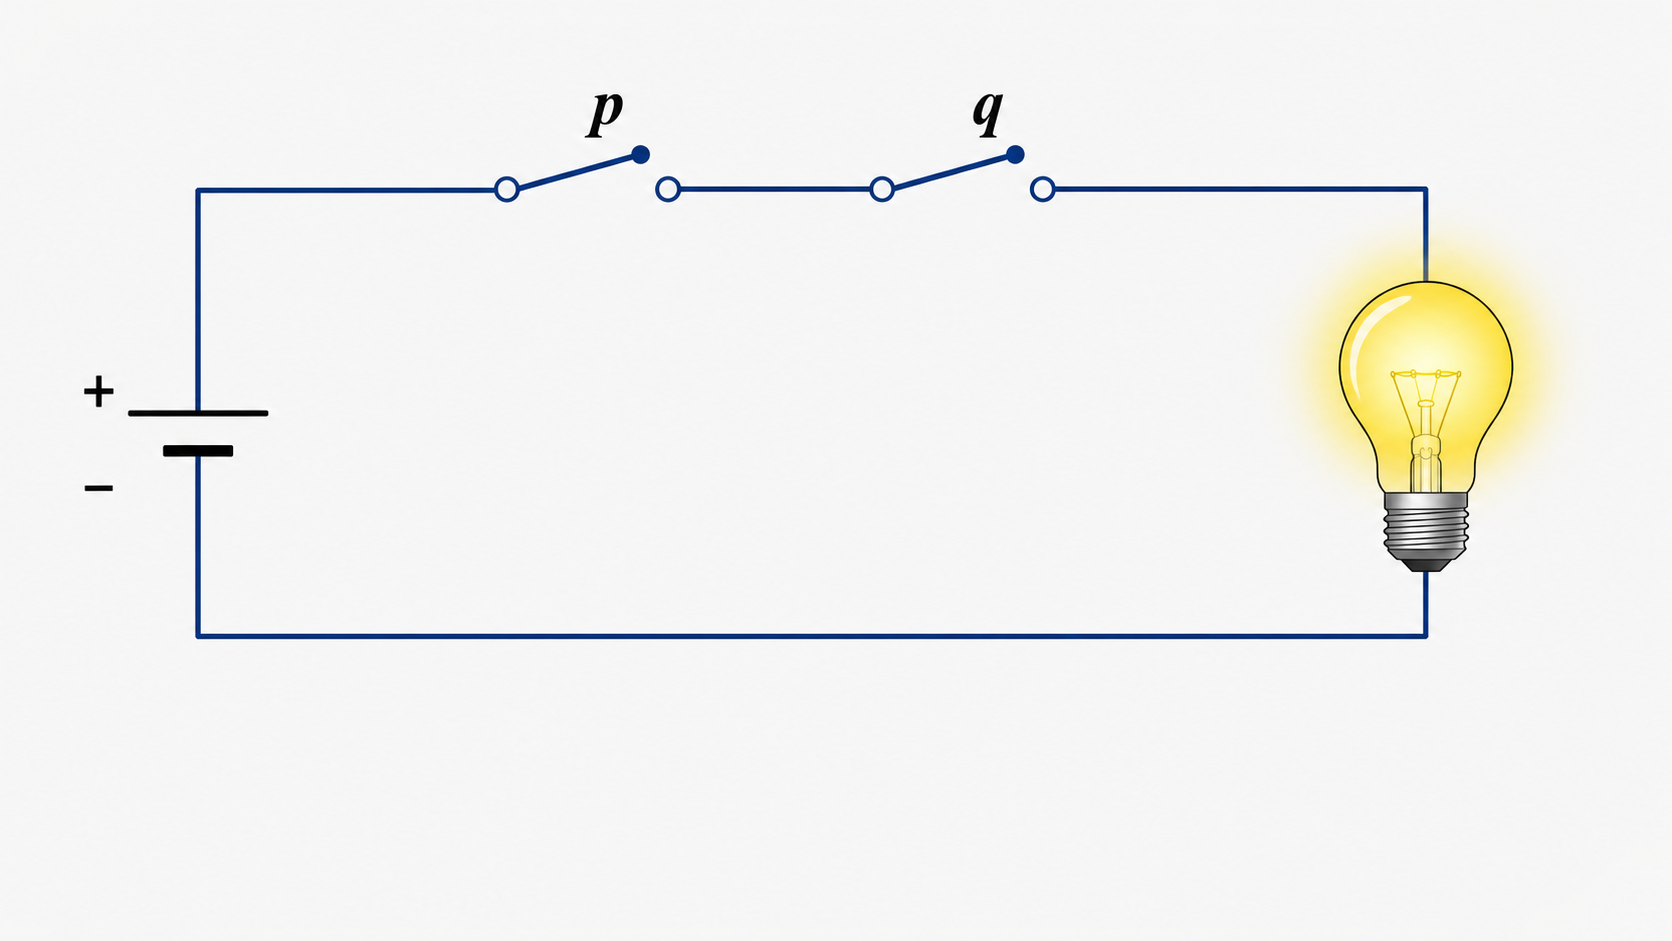
\includegraphics[width=0.8\textwidth]{Figures/02-and-gate-circuit.png}
    \caption{วงจรสวิตช์ไฟฟ้าแบบอนุกรม แสดงการทำงานของ $p \land q$}
    \label{fig:and-gate-circuit}
\end{figure}

\noindent พิจารณาตัวอย่างค่าความจริงของการเชื่อมด้วยคำว่า ``และ'':
\begin{align*}
(2>1) \land (4<5) &\equiv \text{T} \land \text{T} \equiv \text{T}\\
(2+2=5) \land (\text{คนปกติมี 6 ขา}) &\equiv \text{F} \land \text{F} \equiv \text{F}
\end{align*}

\subsection{ประพจน์เลือก (Disjunction / OR, $\lor$)}

ประพจน์เลือก (disjunction, OR) ใช้สัญลักษณ์ $\lor$ ในทางตรรกศาสตร์ และใช้ในวงจรดิจิทัลว่า OR Gate ประพจน์ $p \lor q$ อ่านว่า $p$ หรือ $q$ จะเป็นจริงเมื่อมีอย่างน้อยหนึ่งใน $p$ หรือ $q$ เป็นจริง จะเป็นเท็จก็ต่อเมื่อทั้ง $p$ และ $q$ เป็นเท็จทั้งคู่ ต้องระวังว่า OR ในทางตรรกศาสตร์เป็น OR แบบรวม (Inclusive OR) ซึ่งรวมกรณีที่ทั้งคู่จริงด้วย

\begin{table}[H]
    \centering
    \caption{ประพจน์เลือก ($p \lor q$)}
    \label{tab:or-truth}
    \begin{tabular}{|c|c|c|}
        \hline
        \textbf{$p$} & \textbf{$q$} & \textbf{$p \lor q$} \\ \hline
        T & T & T \\ \hline
        T & F & T \\ \hline
        F & T & T \\ \hline
        F & F & F \\ \hline
    \end{tabular}
\end{table}

\bigskip

\begin{figure}[H]
    \centering
    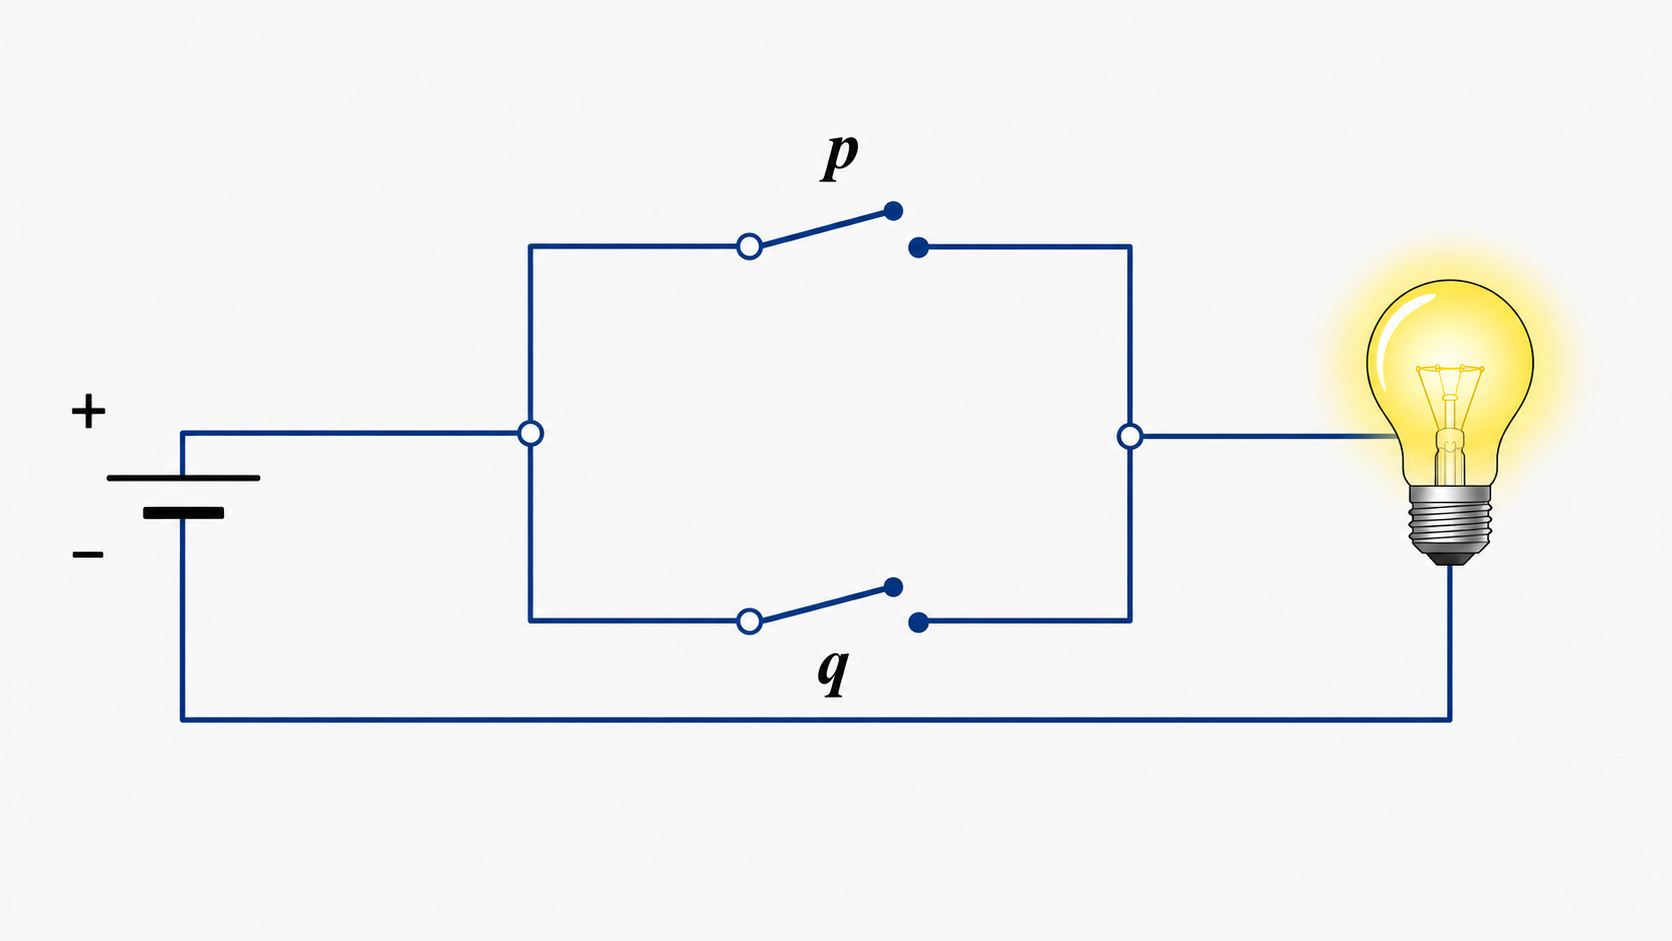
\includegraphics[width=0.8\textwidth]{Figures/03-or-gate-circuit.png}
    \caption{วงจรสวิตช์ไฟฟ้าแบบขนาน แสดงการทำงานของ $p \lor q$}
    \label{fig:or-gate-circuit}
\end{figure}

\noindent พิจารณาตัวอย่างค่าความจริงของการเชื่อมด้วยคำว่า ``หรือ'':
\begin{align*}
(\text{ประเทศไทยอยู่ในทวีปยุโรป}) \lor (2+5>4) &\equiv \text{F} \lor \text{T} \equiv \text{T}\\
(2+2=5) \lor (\text{คนปกติมี 6 ขา}) &\equiv \text{F} \lor \text{F} \equiv \text{F}
\end{align*}

\subsection{นิเสธ (Negation / NOT, $\neg$)}

นิเสธ (Negation) ใช้สัญลักษณ์ $\neg$ เป็นตัวเชื่อมเอกภาพ (Unary Connective) ที่กระทำกับประพจน์เพียงประพจน์เดียว $\neg p$ อ่านว่า ไม่ $p$ หรือ นิเสธของ $p$ การหานิเสธจะกลับค่าความจริงของประพจน์อย่างสมบูรณ์ ถ้า $p$ เป็นจริง $\neg p$ จะเป็นเท็จ และถ้า $p$ เป็นเท็จ $\neg p$ จะเป็นจริง

\begin{table}[H]
    \centering
    \caption{นิเสธ ($\neg p$)}
    \label{tab:not-truth}
    \begin{tabular}{|c|c|}
        \hline
        \textbf{$p$} & \textbf{$\neg p$} \\ \hline
        T & F \\ \hline
        F & T \\ \hline
    \end{tabular}
\end{table}

\subsection{ประพจน์มีเงื่อนไข (Conditional / IMPLIES, $\rightarrow$)}

ประพจน์มีเงื่อนไข (conditional, IMPLIES) ใช้สัญลักษณ์ $\rightarrow$ ประพจน์ $p \rightarrow q$ อ่านว่า ถ้า $p$ แล้ว $q$ โดย $p$ เรียกว่า เงื่อนไขนำ (Antecedent) และ $q$ เรียกว่า เงื่อนไขตาม (Consequent) ค่าความจริงของ $p \rightarrow q$ จะเป็นเท็จเพียงกรณีเดียวคือ เมื่อเงื่อนไขนำ $p$ เป็นจริงแต่เงื่อนไขตาม $q$ เป็นเท็จ

\begin{table}[H]
    \centering
    \caption{ประพจน์มีเงื่อนไข ($p \rightarrow q$)}
    \label{tab:implies-truth}
    \begin{tabular}{|c|c|c|}
        \hline
        \textbf{$p$} & \textbf{$q$} & \textbf{$p \rightarrow q$} \\ \hline
        T & T & T \\ \hline
        T & F & F \\ \hline
        F & T & T \\ \hline
        F & F & T \\ \hline
    \end{tabular}
\end{table}

\bigskip

\begin{figure}[H]
    \centering
    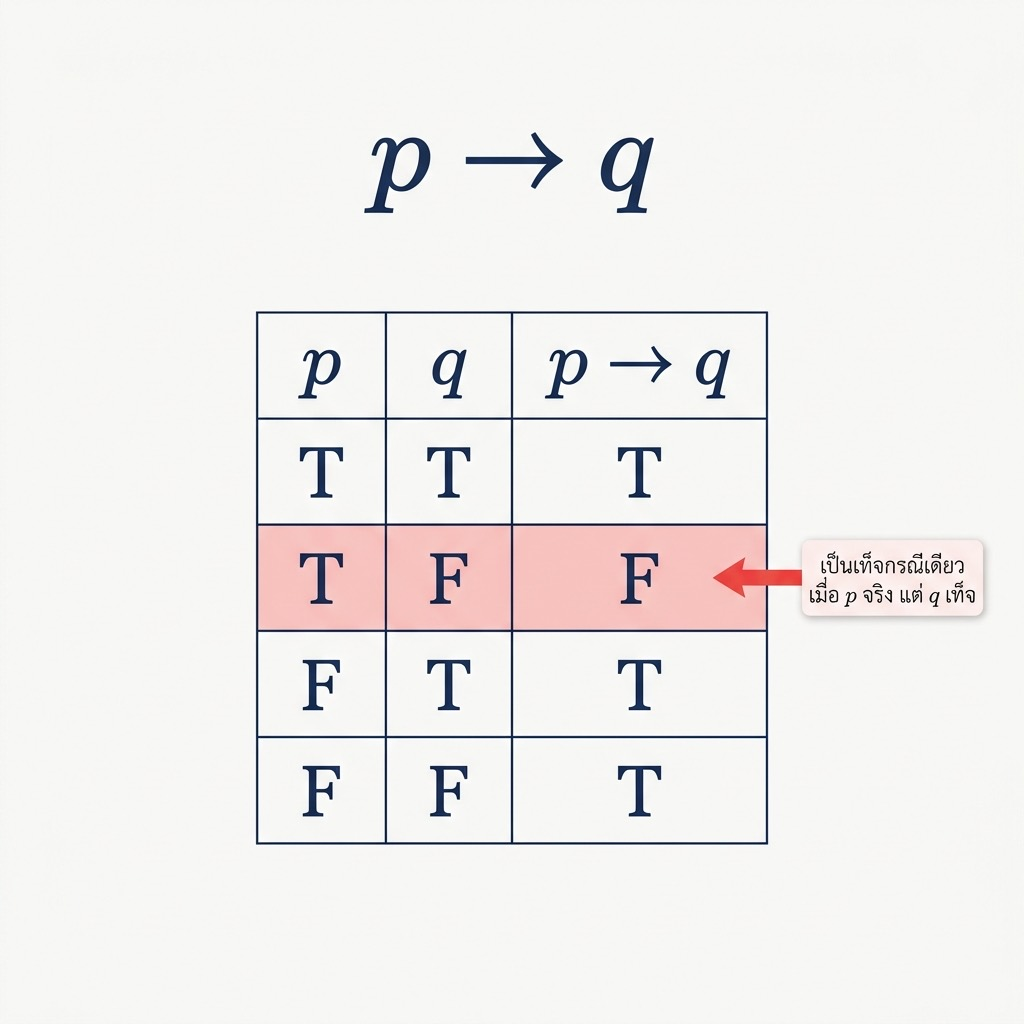
\includegraphics[width=0.8\textwidth]{Figures/04-implication-truth.png}
    \caption{ตารางค่าความจริงของ Implication $p \rightarrow q$ แสดงกรณีที่เป็นเท็จเพียงเมื่อ $p=\text{T}$ แต่ $q=\text{F}$}
    \label{fig:implication-truth}
\end{figure}

\noindent พิจารณาตัวอย่างค่าความจริงของประพจน์มีเงื่อนไข:
\begin{align*}
(\text{เป็นคนปกติ}) \rightarrow (\text{มี 2 ตา}) &\equiv \text{T} \rightarrow \text{T} \equiv \text{T}\\
(\text{เป็นคนปกติ}) \rightarrow (\text{มี 6 ขา}) &\equiv \text{T} \rightarrow \text{F} \equiv \text{F}\\
(\text{หมูบินได้}) \rightarrow (\text{สอบได้ที่หนึ่ง}) &\equiv \text{T} \quad (\text{เงื่อนไขนำเป็นเท็จ})
\end{align*}

\subsection{ประพจน์เงื่อนไขสองทาง (Biconditional / IFF, $\leftrightarrow$)}

ประพจน์เงื่อนไขสองทาง (biconditional, IFF) ใช้สัญลักษณ์ $\leftrightarrow$ ประพจน์ $p \leftrightarrow q$ อ่านว่า ``$p$ ก็ต่อเมื่อ $q$'' หมายความว่า $p$ และ $q$ มีค่าความจริงเหมือนกัน (จริงทั้งคู่หรือเท็จทั้งคู่) IFF เป็นการรวมกันของ $p \rightarrow q$ และ $q \rightarrow p$ ซึ่งสมมูลกับ $(p \rightarrow q) \land (q \rightarrow p)$

\begin{table}[H]
    \centering
    \caption{เงื่อนไขสองทาง ($p \leftrightarrow q$)}
    \label{tab:iff-truth}
    \begin{tabular}{|c|c|c|}
        \hline
        \textbf{$p$} & \textbf{$q$} & \textbf{$p \leftrightarrow q$} \\ \hline
        T & T & T \\ \hline
        T & F & F \\ \hline
        F & T & F \\ \hline
        F & F & T \\ \hline
    \end{tabular}
\end{table}

\bigskip

\noindent พิจารณาตัวอย่างค่าความจริงของการเชื่อมด้วยคำว่า ``ก็ต่อเมื่อ'':
\begin{align*}
(2+2=4) \leftrightarrow (3<5) &\equiv \text{T} \leftrightarrow \text{T} \equiv \text{T}\\
(2+2=5) \leftrightarrow (\text{คนปกติมี 6 ขา}) &\equiv \text{F} \leftrightarrow \text{F} \equiv \text{T}\\
(2+2=4) \leftrightarrow (\text{คนปกติมี 6 ขา}) &\equiv \text{T} \leftrightarrow \text{F} \equiv \text{F}
\end{align*}

\noindent ในทางตรรกศาสตร์ การเชื่อมแบบก็ต่อเมื่อมีความสัมพันธ์อย่างใกล้ชิดกับการเชื่อมแบบถ้า...แล้วสองทิศทาง กล่าวคือ $p \leftrightarrow q$ สมมูลกับ $(p \rightarrow q) \land (q \rightarrow p)$ ความสมมูลนี้มีความสำคัญในการพิสูจน์ทางคณิตศาสตร์และการแปลงประพจน์เชิงตรรกศาสตร์

\begin{prop}
\index{สมมูล!biconditional}
สำหรับทุกประพจน์ $p$ และ $q$ จะได้ว่า
\begin{equation}
p \leftrightarrow q \equiv (p \rightarrow q) \land (q \rightarrow p)
\end{equation}
โดยที่ $p$ และ $q$ เป็นประพจน์ใดๆ, $\rightarrow$ คือตัวเชื่อมแบบถ้า...แล้วที่จะเท็จเพียงกรณีเดียวคือเมื่อเงื่อนไขนำเป็นจริงแต่เงื่อนไขตามเป็นเท็จ และ $\land$ คือตัวเชื่อมแบบและที่จะจริงเมื่อทั้งสองประพจน์เป็นจริง
\end{prop}

\begin{table}[h]
    \centering
    \caption{ตารางพิสูจน์ความสมมูลของ Biconditional}
    \label{tab:biconditional-equiv}
    \begin{tabular}{|c|c|c|c|c|c|}
        \hline
        \textbf{$p$} & \textbf{$q$} & \textbf{$p \rightarrow q$} & \textbf{$q \rightarrow p$} & \textbf{$(p \rightarrow q) \land (q \rightarrow p)$} & \textbf{$p \leftrightarrow q$} \\ \hline
        T & T & T & T & T & T \\ \hline
        T & F & F & T & F & F \\ \hline
        F & T & T & F & F & F \\ \hline
        F & F & T & T & T & T \\ \hline
    \end{tabular}
\end{table}

ตารางที่ \ref{tab:biconditional-equiv} แสดงให้เห็นว่าคอลัมน์ $(p \rightarrow q) \land (q \rightarrow p)$ และ $p \leftrightarrow q$ มีค่าเหมือนกันทุกแถว จึงสรุปได้ว่า $p \leftrightarrow q \equiv (p \rightarrow q) \land (q \rightarrow p)$ ตามที่ต้องการพิสูจน์

\bigskip

\begin{ex}[การหาค่าความจริงของประพจน์]
พิจารณาประพจน์ $(\neg p \land q) \rightarrow r$ จงหาค่าความจริงเมื่อ $p = \text{F}$, $q = \text{T}$, และ $r = \text{F}$
\end{ex}

\begin{solution}
แทนค่า $p = \text{F}$, $q = \text{T}$, และ $r = \text{F}$ ลงในประพจน์เพื่อหาค่าความจริงได้ผลลัพธ์ดังนี้
\begin{align*}
    (\neg p \land q) \rightarrow r &\equiv (\neg \text{F} \land \text{T}) \rightarrow \text{F} \\
    &\equiv (\text{T} \land \text{T}) \rightarrow \text{F} \\
    &\equiv \text{T} \rightarrow \text{F} \\
    &\equiv \text{F}
\end{align*}
ดังนั้น ประพจน์มีค่าความจริงเป็น เท็จ (F)
\end{solution}

\section{สัจนิรันดร์และข้อขัดแย้ง}
\index{สัจนิรันดร์}
\index{Contradiction}
\index{Contingency}
\zlabel{sec:tautology}

เมื่อศึกษาประพจน์เชิงประกอบแล้ว คำถามสำคัญคือ ประพจน์เชิงประกอบนั้นมีค่าความจริงเป็นอย่างไรโดยรวม กล่าวคือ ในทุกกรณีของค่าความจริงของตัวแปรย่อย ประพจน์เชิงประกอบจะมีค่าความจริงเป็นจริงเสมอ หรือเป็นเท็จเสมอ หรือขึ้นกับกรณี การจำแนกประพจน์เชิงประกอบตามลักษณะนี้มีความสำคัญมากในทางคณิตศาสตร์และการพิสูจน์

สัจนิรันดร์ (Tautology) หมายถึง ประพจน์เชิงประกอบที่มีค่าความจริงเป็นจริงในทุกกรณีของการกำหนดค่าความจริงของตัวแปรย่อย ความรู้เรื่องสัจนิรันดร์มีความสำคัญอย่างยิ่งในการพิสูจน์ทางคณิตศาสตร์ เนื่องจากประพจน์ที่เป็นสัจนิรันดร์ถือว่าเป็นความจริงที่จำเป็น (Necessary Truth) ไม่ว่าสถานการณ์จริงเป็นอย่างไรก็ตาม

ในทางตรงกันข้าม ข้อขัดแย้ง (Contradiction) หมายถึง ประพจน์เชิงประกอบที่ไม่มีทางเป็นจริงได้เลย ไม่ว่าค่าความจริงของตัวแปรย่อยจะถูกกำหนดให้เป็นอะไรก็ตาม กล่าวคือ ประพจน์ข้อขัดแย้งจะมีค่าความจริงเป็นเท็จในทุกกรณี ตัวอย่างที่เห็นได้ชัดคือ $p \land \neg p$ ซึ่งสะท้อนหลักการที่ว่า $p$ กับ $\neg p$ ไม่อาจเป็นจริงพร้อมกันได้

สำหรับประพจน์กลาง (Contingency) คือ ประพจน์เชิงประกอบที่มีค่าความจริงเป็นจริงบ้างและเป็นเท็จบ้าง ขึ้นอยู่กับค่าของตัวแปรย่อย ประพจน์ส่วนใหญ่ในชีวิตจริงเป็นประพจน์กลาง

\subsection{สัจนิรันดร์ (Tautology)}
ประพจน์เชิงประกอบบางรูปแบบให้ค่าความจริงเป็นจริงทุกแถวของตารางค่าความจริง ไม่ว่าจะแทนค่าตัวแปรย่อยด้วยจริงหรือเท็จอย่างไร ประพจน์ลักษณะนี้เรียกว่าสัจนิรันดร์

\begin{definition}[สัจนิรันดร์]
\index{สัจนิรันดร์!นิยาม}
สัจนิรันดร์ (Tautology) คือ ประพจน์เชิงประกอบที่มีค่าความจริงเป็นจริงในทุกกรณีของการกำหนดค่าความจริงของตัวแปรย่อย
\end{definition}

ตัวอย่างที่ง่ายที่สุดของสัจนิรันดร์คือ $p \lor \neg p$ ซึ่งอ่านว่า $p$ หรือไม่ $p$ ประพจน์นี้เป็นจริงเสมอ เนื่องจากในทุกสถานการณ์ $p$ จะต้องเป็นจริงหรือเท็จอย่างใดอย่างหนึ่ง จึงทำให้ $p \lor \neg p$ เป็นจริงในทุกกรณี ผลลัพธ์นี้สอดคล้องกับกฎกีดกันกลาง (Law of Excluded Middle) ของอริสโตเติล~\cite{aristotle_organon} ซึ่งระบุว่าสำหรับทุกประพจน์ $p$ แล้ว $p$ หรือ $\neg p$ จะต้องเป็นจริงอย่างน้อยหนึ่งอย่าง

\begin{table}[h]
    \centering
    \caption{ตารางแสดงว่า $p \lor \neg p$ เป็นสัจนิรันดร์}
    \label{tab:tautology-law-excluded}
    \begin{tabular}{|c|c|c|}
        \hline
        \textbf{$p$} & \textbf{$\neg p$} & \textbf{$p \lor \neg p$} \\ \hline
        T & F & T \\ \hline
        F & T & T \\ \hline
    \end{tabular}
\end{table}

ตารางที่ \ref{tab:tautology-law-excluded} แสดงให้เห็นว่าคอลัมน์สุดท้ายมีค่า T ทุกแถว จึงเป็นสัจนิรันดร์

ตัวอย่างสัจนิรันดร์อื่นๆ ได้แก่ $p \rightarrow p$ ซึ่งหมายความว่าถ้า $p$ แล้ว $p$ ย่อมจริงเสมอ $p \leftrightarrow p$ ซึ่งหมายความว่า $p$ ก็ต่อเมื่อ $p$ และ $(p \land q) \rightarrow p$ ซึ่งหมายความว่าถ้า $p$ และ $q$ เป็นจริง แล้ว $p$ ย่อมจริง

\begin{table}[h]
    \centering
    \caption{ตารางแสดงว่า $(p \land q) \rightarrow p$ เป็นสัจนิรันดร์}
    \label{tab:tautology-absorption}
    \begin{tabular}{|c|c|c|c|c|}
        \hline
        \textbf{$p$} & \textbf{$q$} & \textbf{$p \land q$} & \textbf{$(p \land q) \rightarrow p$} & \textbf{ผลลัพธ์} \\ \hline
        T & T & T & T & T \\ \hline
        T & F & F & T & T \\ \hline
        F & T & F & T & T \\ \hline
        F & F & F & T & T \\ \hline
    \end{tabular}
\end{table}

ตารางที่ \ref{tab:tautology-absorption} แสดงให้เห็นว่า $(p \land q) \rightarrow p$ เป็นจริงทุกกรณี

การพิสูจน์โดยการใช้สัจนิรันดร์ ในการพิสูจน์ทางคณิตศาสตร์ หากต้องการแสดงว่าข้อความ $P$ เป็นจริง อาจพิสูจน์ว่า $\neg P$ นำไปสู่ข้อขัดแย้ง (Contradiction) เมื่อ $\neg P$ นำไปสู่ข้อขัดแย้ง แสดงว่า $\neg P$ เป็นเท็จ จึงสรุปได้ว่า $P$ เป็นจริง วิธีนี้เรียกว่า การพิสูจน์โดยข้อขัดแย้ง (Proof by Contradiction) ตัวอย่างต่อไปนี้เป็นตัวอย่างคลาสสิกที่ใช้เทคนิคดังกล่าว จึงควรอ่านในฐานะสะพานเชื่อมระหว่างตรรกศาสตร์กับวิธีพิสูจน์ทางคณิตศาสตร์

\begin{ex}[การพิสูจน์โดยข้อขัดแย้ง]
จงพิสูจน์ว่า $\sqrt{2}$ เป็นจำนวนอตรรกยะ
\end{ex}

\begin{solution}
สมมติในทางตรงข้ามว่า $\sqrt{2}$ เป็นจำนวนตรรกยะ จะเขียนได้เป็น $\sqrt{2} = \dfrac{a}{b}$ โดย $a,b \in \mathbb{Z}$, $b \neq 0$ และ $\gcd(a,b)=1$
\begin{align*}
\sqrt{2} = \frac{a}{b} \ &\Rightarrow\ 2 = \frac{a^2}{b^2} \ \Rightarrow\ a^2 = 2b^2 \quad (a^2 \text{ คู่} \Rightarrow a \text{ คู่})\\
a = 2c \ &\Rightarrow\ (2c)^2 = 2b^2 \ \Rightarrow\ b^2 = 2c^2 \quad (b^2 \text{ คู่} \Rightarrow b \text{ คู่})
\end{align*}
แต่ $a$ และ $b$ เป็นจำนวนคู่ทั้งคู่ ขัดแย้งกับ $\gcd(a,b)=1$ ดังนั้นข้อสมมติเป็นเท็จ จึงสรุปว่า $\sqrt{2}$ เป็นจำนวนอตรรกยะ \solhere
\end{solution}

การพิสูจน์นี้ใช้หลักการว่า ถ้า $\neg P$ นำไปสู่ข้อขัดแย้ง แสดงว่า $P$ เป็นจริง

\subsection{ข้อขัดแย้ง (Contradiction)}
ในทางกลับกัน ประพจน์เชิงประกอบบางรูปแบบให้ค่าความจริงเป็นเท็จทุกแถวของตารางค่าความจริง ไม่ว่าจะแทนค่าตัวแปรย่อยอย่างไร ประพจน์ลักษณะนี้เรียกว่าข้อขัดแย้ง

\begin{definition}[ข้อขัดแย้ง]
\index{ข้อขัดแย้ง!นิยาม}
ข้อขัดแย้ง (Contradiction) คือ ประพจน์เชิงประกอบที่ไม่มีทางเป็นจริงได้ ไม่ว่าค่าความจริงของตัวแปรย่อยจะถูกกำหนดให้เป็นอะไรก็ตาม ประพจน์ที่เป็นข้อขัดแย้งจะมีค่าความจริงเป็นเท็จเสมอ
\end{definition}

ตัวอย่างที่ง่ายที่สุดของข้อขัดแย้งคือ $p \land \neg p$ ซึ่งอ่านว่า $p$ และไม่ $p$ ประพจน์นี้เป็นเท็จเสมอ เนื่องจากประพจน์เดียวกันไม่อาจมีค่าความจริงเป็นทั้งจริงและเท็จในเวลาเดียวกันได้

หลักการนี้สอดคล้องกับกฎแห่งการไม่ขัดแย้ง (Law of Non-Contradiction) ซึ่งระบุว่า $p$ กับ $\neg p$ ไม่อาจเป็นจริงพร้อมกันได้ การเข้าใจข้อขัดแย้งมีความสำคัญในการพิสูจน์ทางคณิตศาสตร์ เนื่องจากเมื่อแสดงว่าข้อสันนิษฐานหนึ่งนำไปสู่ข้อขัดแย้ง ย่อมสรุปได้ว่าข้อสันนิษฐานนั้นต้องเป็นเท็จ

\begin{table}[h]
    \centering
    \caption{ตารางแสดงว่า $p \land \neg p$ เป็นข้อขัดแย้ง}
    \label{tab:contradiction}
    \begin{tabular}{|c|c|c|c|}
        \hline
        \textbf{$p$} & \textbf{$\neg p$} & \textbf{$p \land \neg p$} & \textbf{ผลลัพธ์} \\ \hline
        T & F & F & F \\ \hline
        F & T & F & F \\ \hline
    \end{tabular}
\end{table}

ตารางที่ \ref{tab:contradiction} แสดงให้เห็นว่าคอลัมน์สุดท้ายมีค่า F ทุกแถว จึงเป็นข้อขัดแย้ง

ตัวอย่างข้อขัดแย้งอื่นๆ ได้แก่ $\neg(p \lor \neg p)$ ซึ่งเป็นนิเสธของกฎกีดกันกลาง และ $(p \rightarrow q) \land (p \land \neg q)$ ซึ่งหมายความว่า $q$ ต้องเป็นจริงและเท็จพร้อมกันภายใต้เงื่อนไขเดียวกัน

หากพบว่าการสันนิษฐานนำไปสู่ข้อขัดแย้ง แสดงว่าการสันนิษฐานนั้นเป็นเท็จ นี่คือหลักการพื้นฐานของการพิสูจน์โดยข้อขัดแย้ง (Proof by Contradiction) ซึ่งเป็นเทคนิคพื้นฐานในทางคณิตศาสตร์

ความสัมพันธ์ระหว่างสัจนิรันดร์และข้อขัดแย้งมีความสำคัญ โดยนิเสธของสัจนิรันดร์คือข้อขัดแย้ง และนิเสธของข้อขัดแย้งคือสัจนิรันดร์ กล่าวคือ ถ้า $P$ เป็นสัจนิรันดร์ แล้ว $\neg P$ จะเป็นข้อขัดแย้ง และถ้า $P$ เป็นข้อขัดแย้ง แล้ว $\neg P$ จะเป็นสัจนิรันดร์

\subsection{ประพจน์กลาง (Contingency)}

ประพจน์กลาง (Contingency) คือ ประพจน์เชิงประกอบที่มีค่าความจริงเป็นจริงบ้างและเป็นเท็จบ้าง ขึ้นอยู่กับค่าความจริงของตัวแปรย่อย กล่าวคือ ไม่เป็นสัจนิรันดร์ก็ไม่เป็นข้อขัดแย้ง แต่มีค่าความจริงขึ้นกับการกำหนดค่าของตัวแปรย่อย ประพจน์ส่วนใหญ่ในชีวิตประจำวันและในคณิตศาสตร์เป็นประพจน์กลาง

\begin{table}[h]
    \centering
    \caption{ตารางแสดงว่า $p \land q$ เป็นประพจน์กลาง}
    \label{tab:contingency-example}
    \begin{tabular}{|c|c|c|c|}
        \hline
        \textbf{$p$} & \textbf{$q$} & \textbf{$p \land q$} & \textbf{ผลลัพธ์} \\ \hline
        T & T & T & T \\ \hline
        T & F & F & F \\ \hline
        F & T & F & F \\ \hline
        F & F & F & F \\ \hline
    \end{tabular}
\end{table}

ตารางที่ \ref{tab:contingency-example} แสดงให้เห็นว่า $p \land q$ ไม่เป็นสัจนิรันดร์ (เพราะมี F) และไม่เป็นข้อขัดแย้ง (เพราะมี T) จึงเป็นประพจน์กลาง

ประพจน์กลางเป็นประพจน์ที่มีความหมายจริงในการใช้งาน เนื่องจากค่าความจริงของประพจน์กลางขึ้นกับข้อเท็จจริงในโลกจริง ตัวอย่างเช่น ประพจน์ วันนี้ฝนตก จะเป็นจริงหรือเท็จขึ้นกับสถานการณ์จริงในวันนั้น

\section{ความสมมูลเชิงตรรกะและกฎพีชคณิตของประพจน์}
\index{ความสมมูลเชิงตรรกะ}
\index{Logical Equivalence}
\label{sec:logical-equivalence}

ในการวิเคราะห์และจัดรูปประพจน์เชิงประกอบ มักพบว่าประพจน์ที่มีรูปแบบสัญลักษณ์แตกต่างกันอาจให้ค่าความจริงเหมือนกันในทุกกรณี ความสัมพันธ์นี้เรียกว่า ความสมมูลเชิงตรรกะ (Logical Equivalence) ซึ่งเป็นแนวคิดที่สำคัญทั้งในการพิสูจน์ทางคณิตศาสตร์ การลดรูปนิพจน์บูลีน และการออกแบบวงจรดิจิทัล

\begin{definition}[ความสมมูลเชิงตรรกะ]
\index{ความสมมูลเชิงตรรกะ!นิยาม}
ประพจน์ $P$ และ $Q$ เรียกว่า สมมูลเชิงตรรกะ (Logically Equivalent) เขียนแทนด้วย $P \equiv Q$ ก็ต่อเมื่อ $P$ และ $Q$ มีค่าความจริงเหมือนกันในทุกกรณีของการกำหนดค่าความจริงของตัวแปรย่อย หรือกล่าวอย่างเทียบเท่าว่า ประพจน์ $P \leftrightarrow Q$ เป็นสัจนิรันดร์
\end{definition}

จากนิยามจะเห็นได้ว่า การตรวจสอบความสมมูลทำได้สองวิธีหลัก คือ สร้างตารางค่าความจริงเปรียบเทียบทีละแถว หรือใช้กฎพีชคณิตของประพจน์ในการแปลงรูปจากด้านหนึ่งให้กลายเป็นอีกด้านหนึ่ง

\subsection{กฎพีชคณิตของประพจน์ (Laws of Propositional Algebra)}
\index{พีชคณิตของประพจน์}

กฎพีชคณิตของประพจน์เป็นชุดของความสมมูลพื้นฐานที่ใช้บ่อยในการลดรูปและพิสูจน์ทฤษฎีบทเชิงตรรกะ อันที่จริงกฎเหล่านี้เป็น \emph{กรณีรูปธรรม} ของกฎในพีชคณิตบูลีน (Boolean Algebra) ซึ่งเป็นโครงสร้างนามธรรมที่จะได้ศึกษาอย่างละเอียดใน\autoref{ch:boolean} (กฎชุดเดียวกันนี้ยังปรากฏในทฤษฎีเซตอีกด้วย ดังจะเห็นใน\autoref{ch:set}) ตารางที่ \ref{tab:propositional-laws} สรุปกฎที่สำคัญทั้งหมด

\begin{table}[h]
    \centering
    \caption{กฎพีชคณิตของประพจน์ (โดยที่ $T$ แทนสัจนิรันดร์ และ $F$ แทนข้อขัดแย้ง)}
    \label{tab:propositional-laws}
    \begin{tabular}{|l|l|}
        \hline
        \textbf{ชื่อกฎ} & \textbf{รูปสมมูล} \\ \hline
        กฎเอกลักษณ์ (Identity) & $p \land T \equiv p$, \quad $p \lor F \equiv p$ \\ \hline
        กฎครอบงำ (Domination) & $p \lor T \equiv T$, \quad $p \land F \equiv F$ \\ \hline
        กฎนิจพล (Idempotent) & $p \lor p \equiv p$, \quad $p \land p \equiv p$ \\ \hline
        กฎนิเสธซ้อน (Double Negation) & $\neg(\neg p) \equiv p$ \\ \hline
        กฎสลับที่ (Commutative) & $p \lor q \equiv q \lor p$, \quad $p \land q \equiv q \land p$ \\ \hline
        กฎเปลี่ยนกลุ่ม (Associative) & $(p \lor q) \lor r \equiv p \lor (q \lor r)$ \\ \hline
                                     & $(p \land q) \land r \equiv p \land (q \land r)$ \\ \hline
        กฎแจกแจง (Distributive) & $p \lor (q \land r) \equiv (p \lor q) \land (p \lor r)$ \\ \hline
                                & $p \land (q \lor r) \equiv (p \land q) \lor (p \land r)$ \\ \hline
        กฎเดอมอร์แกน (De Morgan) & $\neg(p \land q) \equiv \neg p \lor \neg q$ \\ \hline
                                 & $\neg(p \lor q) \equiv \neg p \land \neg q$ \\ \hline
        กฎดูดกลืน (Absorption) & $p \lor (p \land q) \equiv p$, \quad $p \land (p \lor q) \equiv p$ \\ \hline
        กฎนิเสธ (Negation) & $p \lor \neg p \equiv T$, \quad $p \land \neg p \equiv F$ \\ \hline
        กฎเงื่อนไข (Implication) & $p \rightarrow q \equiv \neg p \lor q$ \\ \hline
        กฎกระจายเงื่อนไข (Exportation) & $(p \land q) \rightarrow r \equiv p \rightarrow (q \rightarrow r)$ \\ \hline
    \end{tabular}
\end{table}

ตารางที่ \ref{tab:propositional-laws} สรุปกฎพื้นฐานของพีชคณิตของประพจน์ที่ใช้บ่อยที่สุด กฎเหล่านี้สามารถพิสูจน์ได้ทุกข้อด้วยตารางค่าความจริง และจะถูกนำไปใช้ใน\autoref{ch:boolean} (พีชคณิตบูลีน) เพื่อออกแบบและลดรูปวงจรดิจิทัล

\begin{ex}[การใช้กฎพีชคณิตในการลดรูป]
จงพิสูจน์ว่า $\neg(p \lor q) \lor (\neg p \land q) \equiv \neg p$ โดยใช้กฎพีชคณิตของประพจน์
\end{ex}

\begin{solution}
\begin{align*}
\neg(p \lor q) \lor (\neg p \land q) &\equiv (\neg p \land \neg q) \lor (\neg p \land q) \quad \text{(กฎเดอมอร์แกน)} \\
&\equiv \neg p \land (\neg q \lor q) \quad \text{(กฎแจกแจง)} \\
&\equiv \neg p \land T \quad \text{(กฎนิเสธ)} \\
&\equiv \neg p \quad \text{(กฎเอกลักษณ์)}
\end{align*}
ดังนั้น $\neg(p \lor q) \lor (\neg p \land q) \equiv \neg p$
\end{solution}

\subsection{ประพจน์กลับ ประพจน์ผกผัน และประพจน์แย้งสลับที่ (Converse, Inverse, Contrapositive)}
\index{Converse}
\index{Inverse}
\index{Contrapositive}
\index{ผกผัน}
\index{แย้งสลับที่}

ประพจน์เงื่อนไข $p \rightarrow q$ มีประพจน์ที่เกี่ยวข้องกันอย่างใกล้ชิดอีกสามรูปแบบ ซึ่งใช้ในการพิสูจน์ทางคณิตศาสตร์ โดยเฉพาะการพิสูจน์โดยแย้งสลับที่ (Proof by Contrapositive)

\begin{definition}[Converse, Inverse, Contrapositive]
\index{ประพจน์เงื่อนไข!converse}
กำหนดประพจน์เงื่อนไข $p \rightarrow q$
\begin{itemize}
    \item ส่วนกลับ (Converse) คือ $q \rightarrow p$
    \item ผกผัน (Inverse) คือ $\neg p \rightarrow \neg q$
    \item แย้งสลับที่ (Contrapositive) คือ $\neg q \rightarrow \neg p$
\end{itemize}
\end{definition}

ความสัมพันธ์ที่สำคัญที่สุดของประพจน์ทั้งสี่นี้คือ ประพจน์เงื่อนไขกับแย้งสลับที่สมมูลกันเสมอ ในขณะที่ส่วนกลับและผกผันก็สมมูลกันเสมอ แต่ประพจน์เงื่อนไขกับส่วนกลับ \textbf{ไม่สมมูล} กันโดยทั่วไป การสับสนระหว่างประพจน์เงื่อนไขกับส่วนกลับเป็นข้อผิดพลาดเชิงตรรกะที่พบบ่อย (เรียกว่า Affirming the Consequent)

\begin{table}[h]
    \centering
    \caption{ตารางพิสูจน์ความสมมูลของประพจน์เงื่อนไขและแย้งสลับที่}
    \label{tab:contrapositive}
    \begin{tabular}{|c|c|c|c|c|c|}
        \hline
        \textbf{$p$} & \textbf{$q$} & \textbf{$\neg p$} & \textbf{$\neg q$} & \textbf{$p \rightarrow q$} & \textbf{$\neg q \rightarrow \neg p$} \\ \hline
        T & T & F & F & T & T \\ \hline
        T & F & F & T & F & F \\ \hline
        F & T & T & F & T & T \\ \hline
        F & F & T & T & T & T \\ \hline
    \end{tabular}
\end{table}

ตารางที่ \ref{tab:contrapositive} แสดงให้เห็นว่า $p \rightarrow q$ และ $\neg q \rightarrow \neg p$ มีค่าความจริงเหมือนกันทุกแถว จึงสรุปได้ว่า $p \rightarrow q \equiv \neg q \rightarrow \neg p$

\begin{ex}[การเขียน Converse, Inverse, Contrapositive]
กำหนดประพจน์ ``ถ้า $n$ เป็นจำนวนเฉพาะที่มากกว่า 2 แล้ว $n$ เป็นจำนวนคี่'' จงเขียนส่วนกลับ ผกผัน และแย้งสลับที่ของประพจน์นี้
\end{ex}

\begin{solution}
ให้ $p \equiv $ ``$n$ เป็นจำนวนเฉพาะที่มากกว่า 2'' และ $q \equiv$ ``$n$ เป็นจำนวนคี่''
\begin{itemize}
    \item ส่วนกลับ ถ้า $n$ เป็นจำนวนคี่ แล้ว $n$ เป็นจำนวนเฉพาะที่มากกว่า 2 \quad (เป็นเท็จ เช่น $n=9$)
    \item ผกผัน ถ้า $n$ ไม่เป็นจำนวนเฉพาะที่มากกว่า 2 แล้ว $n$ ไม่เป็นจำนวนคี่ \quad (เป็นเท็จ เช่น $n=9$)
    \item แย้งสลับที่ ถ้า $n$ ไม่เป็นจำนวนคี่ แล้ว $n$ ไม่เป็นจำนวนเฉพาะที่มากกว่า 2 \quad (เป็นจริง สมมูลกับประพจน์เดิม)
\end{itemize}
\end{solution}

\section{ตัวเชื่อมเพิ่มเติม: XOR, NAND, NOR}
\index{XOR}
\index{NAND}
\index{NOR}
\zlabel{sec:extended-connectives}

นอกจากตัวเชื่อมพื้นฐาน 5 ตัวที่ได้ศึกษามาแล้ว ยังมีตัวเชื่อมอีกหลายตัวที่นิยมใช้ในวงจรดิจิทัลและวิทยาการคอมพิวเตอร์ ตัวเชื่อมเหล่านี้สามารถนิยามได้จากตัวเชื่อมพื้นฐาน 5 ตัว แต่การมีสัญลักษณ์เฉพาะช่วยให้การเขียนนิพจน์กระชับและเข้าใจง่ายขึ้น

\subsection{ประพจน์เลือกเฉพาะ (Exclusive OR, XOR, $\oplus$)}
\index{XOR!Exclusive OR}

Exclusive OR หรือเรียกย่อว่า XOR ใช้สัญลักษณ์ $\oplus$ เป็นตัวเชื่อมที่ให้ค่าจริงเมื่อประพจน์ทั้งสองมีค่าความจริงต่างกันเท่านั้น แตกต่างจาก OR แบบรวม (Inclusive OR, $\lor$) ที่อนุญาตให้ทั้งคู่เป็นจริงได้ XOR เป็นแบบจำลองเชิงตรรกะของคำว่า ``หรือ'' ในความหมายที่ \textit{เลือกได้อย่างใดอย่างหนึ่งเท่านั้น}

\begin{definition}[Exclusive OR]
\index{XOR!นิยาม}
สำหรับประพจน์ $p$ และ $q$ ใดๆ ประพจน์ $p \oplus q$ มีค่าความจริงเป็นจริงก็ต่อเมื่อ $p$ และ $q$ มีค่าความจริงต่างกัน และเป็นเท็จเมื่อ $p$ กับ $q$ มีค่าความจริงเหมือนกัน หรือเขียนในรูปสมมูลได้ว่า
\begin{equation}
p \oplus q \equiv (p \lor q) \land \neg(p \land q) \equiv (p \land \neg q) \lor (\neg p \land q)
\end{equation}
\end{definition}

\begin{figure}[H]
    \centering
    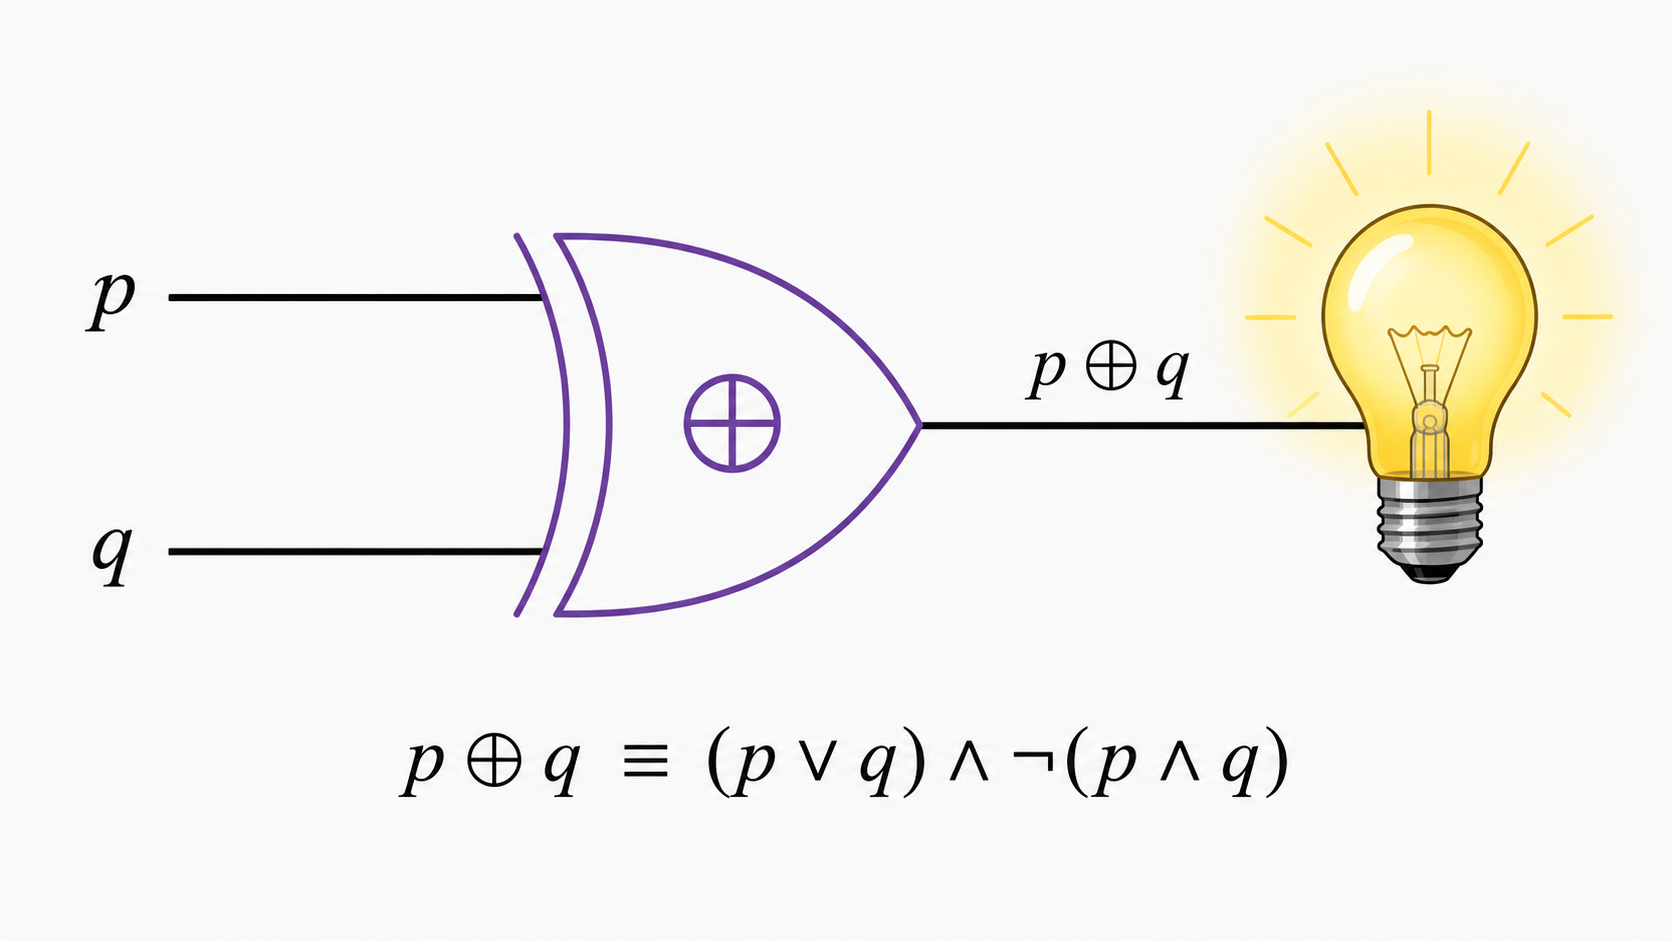
\includegraphics[width=0.85\textwidth]{Figures/09-xor-logic.png}
    \caption{ตารางค่าความจริงและสัญลักษณ์ของลอจิกเกต XOR}
    \label{fig:xor-logic}
\end{figure}

รูปที่ \ref{fig:xor-logic} แสดงตารางค่าความจริงและสัญลักษณ์ของลอจิกเกต XOR ซึ่งให้ผลลัพธ์เป็นจริงเฉพาะเมื่ออินพุตทั้งสองต่างกัน

\begin{table}[h]
    \centering
    \caption{ตารางค่าความจริงของ XOR ($p \oplus q$)}
    \label{tab:xor-truth}
    \begin{tabular}{|c|c|c|}
        \hline
        \textbf{$p$} & \textbf{$q$} & \textbf{$p \oplus q$} \\ \hline
        T & T & F \\ \hline
        T & F & T \\ \hline
        F & T & T \\ \hline
        F & F & F \\ \hline
    \end{tabular}
\end{table}

XOR ใช้ในวิทยาการคอมพิวเตอร์หลายด้าน เช่น
\begin{enumerate}
    \item วงจรบวกเลขฐานสอง (Binary Adder) วงจร Half-Adder ใช้ XOR ในการคำนวณบิตผลรวม (sum bit) ส่วนค่าทด (carry) คำนวณจาก AND
    \item การเข้ารหัสลับ (Cryptography) XOR ถูกนำมาใช้ใน Stream Cipher และ One-Time Pad เพราะมีคุณสมบัติย้อนกลับได้ในตัวเอง กล่าวคือ ถ้า $C = M \oplus K$ แล้ว $M = C \oplus K$ เมื่อ $M$ คือข้อความ $K$ คือกุญแจ และ $C$ คือข้อความที่เข้ารหัสแล้ว
    \item การตรวจสอบความถูกต้องของข้อมูล (Parity Check) ใช้ XOR ของบิตทั้งหมดเพื่อสร้างบิตตรวจสอบ (parity bit) สำหรับตรวจจับความผิดพลาดในการส่งข้อมูล
    \item การสลับค่าตัวแปร (Swap without Temporary Variable) เทคนิคในการเขียนโปรแกรมที่สลับค่าระหว่างตัวแปรสองตัวโดยไม่ใช้ตัวแปรชั่วคราว ผ่านการประยุกต์ XOR สามครั้ง
\end{enumerate}

\subsection{แนนด์และนอร์ (NAND $\uparrow$, NOR $\downarrow$)}
\index{NAND}
\index{NOR}
\index{Universal Gate}

NAND และ NOR เป็นนิเสธของ AND และ OR ตามลำดับ จุดเด่นของตัวเชื่อมทั้งสองคือ คุณสมบัติเป็น \textbf{ตัวเชื่อมสากล (Universal Connective)} หรือในวงจรดิจิทัลเรียกว่า \textbf{Universal Gate} กล่าวคือ สามารถใช้ NAND เพียงอย่างเดียว หรือ NOR เพียงอย่างเดียว ในการสร้างตัวเชื่อมพื้นฐานทั้งหมด (NOT, AND, OR) และจึงสร้างวงจรดิจิทัลใดๆ ก็ได้ คุณสมบัตินี้เป็นเหตุผลสำคัญที่ทำให้การผลิตชิปนิยมใช้ NAND gate เป็นหลัก เพราะลดความซับซ้อนของกระบวนการผลิต

\begin{definition}[NAND และ NOR]
\index{NAND!นิยาม}
\index{NOR!นิยาม}
สำหรับประพจน์ $p$ และ $q$ ใดๆ
\begin{align*}
p \uparrow q &\equiv \neg(p \land q) \quad \text{(NAND, Sheffer stroke)} \\
p \downarrow q &\equiv \neg(p \lor q) \quad \text{(NOR, Peirce arrow)}
\end{align*}
\end{definition}

\begin{table}[h]
    \centering
    \caption{ตารางค่าความจริงของ NAND และ NOR}
    \label{tab:nand-nor-truth}
    \begin{tabular}{|c|c|c|c|}
        \hline
        \textbf{$p$} & \textbf{$q$} & \textbf{$p \uparrow q$ (NAND)} & \textbf{$p \downarrow q$ (NOR)} \\ \hline
        T & T & F & F \\ \hline
        T & F & T & F \\ \hline
        F & T & T & F \\ \hline
        F & F & T & T \\ \hline
    \end{tabular}
\end{table}

ตารางที่ \ref{tab:nand-nor-truth} แสดงค่าความจริงของ NAND และ NOR สังเกตว่า NAND เป็นเท็จเพียงกรณีเดียวคือเมื่อ $p$ และ $q$ จริงทั้งคู่ ส่วน NOR เป็นจริงเพียงกรณีเดียวคือเมื่อ $p$ และ $q$ เท็จทั้งคู่

ตัวอย่างการสร้าง NOT จาก NAND เพียงอย่างเดียว: $\neg p \equiv p \uparrow p$ เพราะ $p \uparrow p \equiv \neg(p \land p) \equiv \neg p$ และการสร้าง AND จาก NAND ทำได้โดย $p \land q \equiv (p \uparrow q) \uparrow (p \uparrow q)$ รายละเอียดของการประยุกต์เพิ่มเติมและการออกแบบวงจรลอจิกจะกล่าวถึงใน\autoref{ch:boolean} ว่าด้วยพีชคณิตบูลีน

\section{ประพจน์เปิดและตัวบ่งปริมาณ (Predicates and Quantifiers)}
\index{ตัวบ่งปริมาณ}
\index{Quantifiers}
\index{ประพจน์เปิด}

ประพจน์ที่ศึกษามาทั้งหมดเป็นประโยคที่ระบุค่าความจริงได้แน่นอน แต่ในทางคณิตศาสตร์เรามักพบประโยคที่มีตัวแปร เช่น ``$x > 5$'' ซึ่งยังบอกค่าความจริงไม่ได้จนกว่าจะแทนค่า $x$ ประโยคลักษณะนี้เรียกว่าประพจน์เปิด

\begin{definition}
\textbf{ประพจน์เปิด (Open Proposition / Predicate)} คือประโยคที่มีตัวแปรหนึ่งตัวหรือมากกว่า เขียนแทนด้วย $P(x), Q(x,y), \ldots$ โดยค่าความจริงขึ้นกับค่าของตัวแปรและเอกภพสัมพัทธ์ (domain) ที่ตัวแปรนั้นรับค่าได้
\end{definition}

ตัวอย่างเช่น ให้ $P(x)$ แทน ``$x > 5$'' บนเอกภพสัมพัทธ์ $\mathbb{R}$ จะได้ว่า $P(7)$ เป็นจริง แต่ $P(2)$ เป็นเท็จ การเปลี่ยนประพจน์เปิดให้มีค่าความจริงแน่นอนทำได้โดยใช้ตัวบ่งปริมาณ (Quantifiers) ซึ่งมี 2 ชนิดหลัก

\begin{definition}
\textbf{ตัวบ่งปริมาณสำหรับทั้งหมด (Universal Quantifier)} เขียนแทนด้วย $\forall$ อ่านว่า ``สำหรับทุก'' (for all) โดย $\forall x\, P(x)$ หมายความว่า ``$P(x)$ เป็นจริงสำหรับสมาชิก $x$ ทุกตัวในเอกภพสัมพัทธ์''

\textbf{ตัวบ่งปริมาณสำหรับบางตัว (Existential Quantifier)} เขียนแทนด้วย $\exists$ อ่านว่า ``มีบางตัว'' หรือ ``มีอย่างน้อยหนึ่งตัว'' (there exists) โดย $\exists x\, P(x)$ หมายความว่า ``มีสมาชิก $x$ อย่างน้อยหนึ่งตัวในเอกภพสัมพัทธ์ที่ทำให้ $P(x)$ เป็นจริง''
\end{definition}

\begin{ex}[การตีความตัวบ่งปริมาณ]
กำหนดเอกภพสัมพัทธ์เป็นจำนวนจริง $\mathbb{R}$ จงพิจารณาค่าความจริงของประพจน์ต่อไปนี้
\begin{enumerate}
  \item $\forall x\, (x^2 \geq 0)$
  \item $\exists x\, (x^2 = 4)$
  \item $\forall x\, (x^2 = 4)$
\end{enumerate}
\end{ex}
\begin{solution}
\begin{align*}
\forall x\,(x^2 \geq 0) &\equiv \text{T} \quad (\text{กำลังสองของจำนวนจริงใด ๆ ไม่ติดลบ})\\
\exists x\,(x^2 = 4) &\equiv \text{T} \quad (\text{เช่น } x = 2)\\
\forall x\,(x^2 = 4) &\equiv \text{F} \quad (\text{ตัวอย่างค้าน } x = 0:\ 0 \neq 4)
\end{align*}
\solhere
\end{solution}

ข้อสังเกตสำคัญคือ การแสดงว่า $\forall x\,P(x)$ เป็นเท็จ ทำได้โดยยกตัวอย่างค้าน (counter-example) เพียงตัวเดียว ส่วนการแสดงว่า $\exists x\,P(x)$ เป็นจริง ก็ทำได้โดยยกตัวอย่างที่ใช้ได้เพียงตัวเดียวเช่นกัน

\subsection{นิเสธของตัวบ่งปริมาณ}
การหานิเสธของประพจน์ที่มีตัวบ่งปริมาณเป็นทักษะที่ใช้บ่อยในการพิสูจน์ โดยมีกฎดังนี้
\begin{align*}
  \neg(\forall x\, P(x)) &\equiv \exists x\, \neg P(x) \\
  \neg(\exists x\, P(x)) &\equiv \forall x\, \neg P(x)
\end{align*}
กล่าวคือ เมื่อใส่นิเสธ $\forall$ จะเปลี่ยนเป็น $\exists$ และ $\exists$ จะเปลี่ยนเป็น $\forall$ พร้อมกับใส่นิเสธให้ประพจน์เปิดด้านใน เช่น นิเสธของ ``นักศึกษาทุกคนสอบผ่าน'' คือ ``มีนักศึกษาอย่างน้อยหนึ่งคนที่สอบไม่ผ่าน''

\begin{rem}
สัญลักษณ์ $\forall$ และ $\exists$ จะถูกนำไปใช้อย่างต่อเนื่องในบทถัดไป เช่น การนิยามสมบัติของความสัมพันธ์ใน\autoref{ch:relations} ที่ใช้รูป ``$\forall a \in A : (a,a) \in R$'' และการเขียนเซตแบบบอกเงื่อนไขของสมาชิก
\end{rem}

\section{การอนุมาน (Inference Rules)}
\index{การอนุมาน}
\index{Inference Rules}
\index{Modus Ponens}
\index{Modus Tollens}
\zlabel{sec:inference-rules}

การอนุมาน (Inference Rules) คือ กฎที่ใช้ในการสรุปผลที่สมเหตุสมผลจากเหตุที่กำหนดให้ การอนุมานเป็นเครื่องมือพื้นฐานในการให้เหตุผลแบบนิรนัย (Deductive Reasoning) ซึ่งเริ่มจากหลักการหรือข้อตั้งต้นทั่วไป แล้วสรุปไปยังกรณีเฉพาะ หากใช้การอนุมานอย่างถูกต้อง ผลที่ได้จะเป็นจริงอย่างแน่นอนตราบใดที่ข้อตั้งต้นเป็นจริง

ในทางตรรกศาสตร์ การอนุมานสามารถเขียนเป็นรูปแบบ (Form) ที่ชัดเจน โดยมีข้อตั้งต้น (Premises) และผลสรุป (Conclusion) รูปแบบการอนุมานที่ถูกต้องจะเป็นสัจนิรันดร์ กล่าวคือ ถ้าข้อตั้งต้นทั้งหมดเป็นจริง ผลสรุปจะต้องเป็นจริงเสมอ

การอนุมานมีหลายรูปแบบ แต่ละรูปแบบมีชื่อเรียกเฉพาะและมีการใช้งานที่แตกต่างกัน การเข้าใจรูปแบบต่างๆ ของการอนุมานมีความสำคัญอย่างยิ่งในการให้เหตุผลอย่างมีตรรกะและการเขียนโปรแกรมคอมพิวเตอร์

การที่การอนุมานจะถือว่าสมเหตุสมผลนั้น ประพจน์เชิงประกอบที่เกิดจากการเชื่อมข้อตั้งต้นทั้งหมดด้วยตัวเชื่อม และ ($\land$) แล้วส่งไปยังผลสรุปด้วยตัวเชื่อม ถ้า...แล้ว ($\rightarrow$) จะต้องเป็น \textbf{สัจนิรันดร์ (Tautology)} เสมอ เช่น สำหรับ Modus Ponens ประพจน์ $[(p \rightarrow q) \land p] \rightarrow q$ ต้องเป็นสัจนิรันดร์ และสำหรับ Modus Tollens ประพจน์ $[(p \rightarrow q) \land \neg q] \rightarrow \neg p$ ต้องเป็นสัจนิรันดร์ ซึ่งสามารถพิสูจน์ความสมเหตุสมผลได้ด้วยตารางค่าความจริงในแต่ละหัวข้อย่อยต่อไปนี้

\subsection{กฎโมดัส โพเนนส์ (Modus Ponens)}
\index{Modus Ponens}
\index{โมดัส โพเนนส์}

Modus Ponens หรือ การยืนยัน เป็นรูปแบบการอนุมานที่ใช้บ่อยที่สุดในการให้เหตุผล มีรูปแบบดังนี้

\begin{enumerate}
    \item ถ้า $p$ แล้ว $q$ โดยมีข้อตั้งต้นที่ 1
    \item $p$ และข้อตั้งต้นที่ 2
    \item $\therefore q$ ผลสรุปคือ
\end{enumerate}

อ่านได้ว่า ถ้า $p$ แล้ว $q$ และ $p$ เป็นจริง แล้ว $q$ ต้องเป็นจริง Modus Ponens เป็นการนำเงื่อนไขนำมายืนยันว่าเป็นจริง ทำให้เงื่อนไขตามต้องเป็นจริงตามไปด้วย หลักการนี้เป็นพื้นฐานของการเขียนโปรแกรมแบบ if-then

\begin{figure}[H]
    \centering
    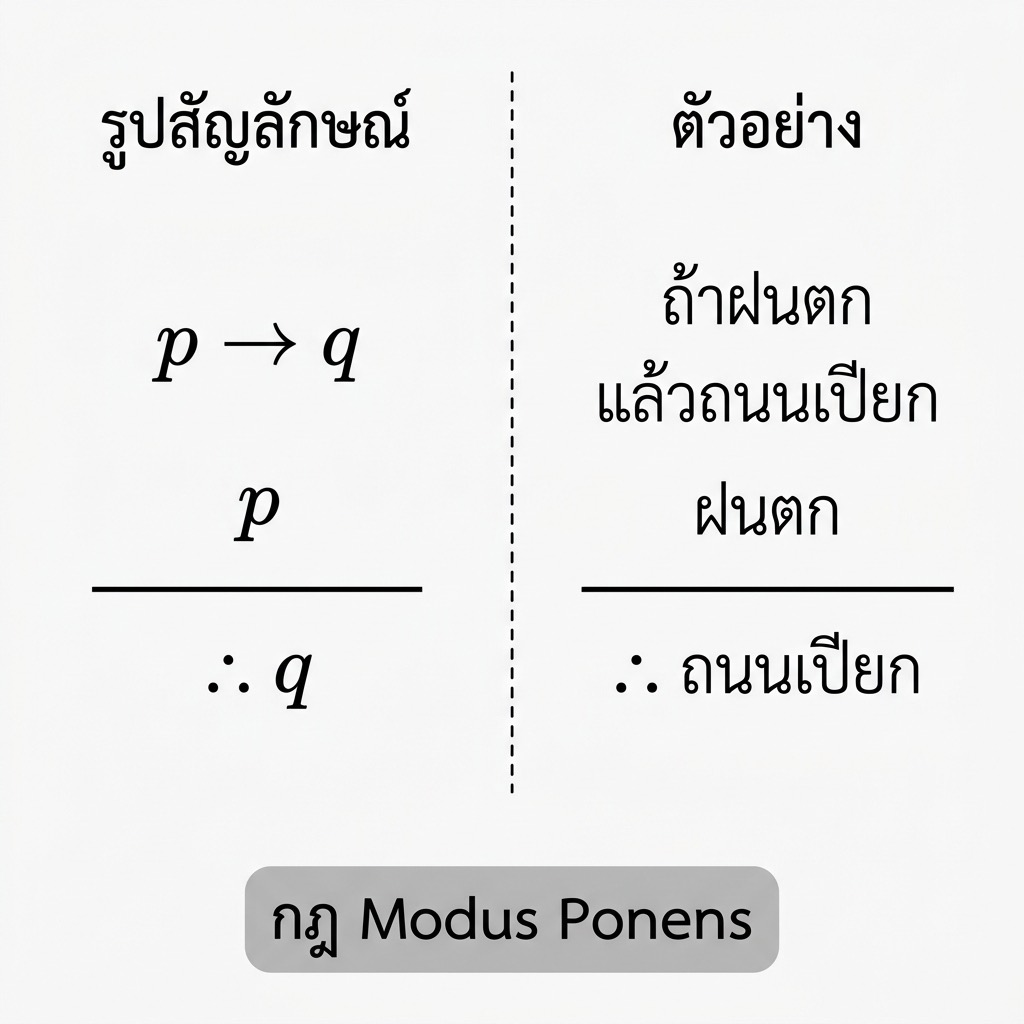
\includegraphics[width=0.85\textwidth]{Figures/07-modus-ponens.png}
    \caption{แผนผังแสดงกฎการอนุมานแบบ Modus Ponens}
    \label{fig:modus-ponens}
\end{figure}

รูปที่ \ref{fig:modus-ponens} แสดงโครงสร้างการอนุมานแบบ Modus Ponens (ละติน: \textit{Modus Ponendo Ponens}) ซึ่งเป็นกฎการอนุมานพื้นฐานในตรรกศาสตร์สัญลักษณ์

\subsubsection{โครงสร้างเชิงตรรกศาสตร์ของ Modus Ponens}
การอนุมานแบบ Modus Ponens ประกอบด้วยข้อตั้งต้น (Premises) 2 ประพจน์ และข้อสรุป (Conclusion) 1 ประพจน์
\begin{enumerate}
    \item ข้อตั้งต้นหลัก (Major Premise) คือประพจน์เงื่อนไข $p \rightarrow q$ ซึ่งระบุความสัมพันธ์ว่าถ้าเงื่อนไขนำ $p$ เกิดขึ้น แล้วเงื่อนไขตาม $q$ จะเกิดตามมา
    \item ข้อตั้งต้นรอง (Minor Premise) คือประพจน์ยืนยันข้อเท็จจริง $p$ ว่าเงื่อนไขนำเกิดขึ้นจริง ($p = T$)
    \item ข้อสรุป (Conclusion) สามารถสรุปผลได้อย่างแน่ชัดว่า $q$ เกิดขึ้นจริง ($\therefore q$)
\end{enumerate}

\subsubsection{การพิสูจน์ความสมเหตุสมผลด้วยตารางค่าความจริง (Tautology Proof)}
การอนุมานแบบ Modus Ponens มีความสมเหตุสมผล (Valid) เนื่องจากรูปแบบประพจน์รวม
\begin{equation}
[(p \rightarrow q) \land p] \rightarrow q
\end{equation}
เป็น \textbf{สัจนิรันดร์ (Tautology)} ซึ่งสามารถพิสูจน์ได้ด้วยตารางค่าความจริงดังตารางที่ \ref{tab:modus-ponens-valid}

\begin{table}[H]
    \centering
    \caption{ตารางค่าความจริงพิสูจน์ความสมเหตุสมผลของ Modus Ponens}
    \label{tab:modus-ponens-valid}
    \begin{tabular}{|c|c|c|c|c|}
        \hline
        $p$ & $q$ & $p \rightarrow q$ & $(p \rightarrow q) \land p$ & $[(p \rightarrow q) \land p] \rightarrow q$ \\ \hline
        \textbf{T} & \textbf{T} & \textbf{T} & \textbf{T} & \textbf{T} \\ \hline
        \textbf{T} & \textbf{F} & \textbf{F} & \textbf{F} & \textbf{T} \\ \hline
        \textbf{F} & \textbf{T} & \textbf{T} & \textbf{F} & \textbf{T} \\ \hline
        \textbf{F} & \textbf{F} & \textbf{T} & \textbf{F} & \textbf{T} \\ \hline
    \end{tabular}
\end{table}

จากตารางที่ \ref{tab:modus-ponens-valid} จะเห็นว่าคอลัมน์สุดท้ายมีค่าความจริงเป็นจริง (T) ในทุกกรณีที่เป็นไปได้ จึงยืนยันได้อย่างเด็ดขาดว่าการให้เหตุผลแบบ Modus Ponens เป็นการอนุมานที่สมเหตุสมผล 100\%

\begin{ex}[การอนุมานแบบ Modus Ponens]
จงหาผลสรุปจากการให้เหตุผลต่อไปนี้ตามหลักเหตุผลทางตรรกศาสตร์
\begin{enumerate}
    \item ถ้าฝนตก แล้วพื้นถนนจะเปียก
    \item ฝนตก
\end{enumerate}
\end{ex}

\begin{solution}
กำหนด $p \equiv \text{ฝนตก}$, $q \equiv \text{พื้นถนนเปียก}$
\[
\begin{array}{r@{\quad}l}
\text{เหตุ 1} & p \rightarrow q\\
\text{เหตุ 2} & p\\
\hline
\therefore & q
\end{array}
\]
นั่นคือ $q \equiv \text{พื้นถนนเปียก}$ \solhere
\end{solution}

จากตัวอย่างจะเห็นว่า เมื่อทราบว่าถ้าฝนตกแล้วพื้นถนนจะเปียก และทราบข้อเท็จจริงว่าฝนตกจริง จึงสรุปได้อย่างแน่ชัดว่าพื้นถนนเปียก

\begin{ex}[การอนุมานแบบ Modus Ponens]
จงหาผลสรุปจากการให้เหตุผลต่อไปนี้ตามหลักเหตุผลทางตรรกศาสตร์
\begin{enumerate}
    \item ถ้าคนรักษาสัญญา แล้วคนนั้นจะได้รับความเชื่อถือ
    \item นาย ก รักษาสัญญา
\end{enumerate}
\end{ex}

\begin{solution}
กำหนด $p \equiv \text{คนรักษาสัญญา}$, $q \equiv \text{ได้รับความเชื่อถือ}$
\[
\begin{array}{r@{\quad}l}
\text{เหตุ 1} & p \rightarrow q\\
\text{เหตุ 2} & p\\
\hline
\therefore & q
\end{array}
\]
นั่นคือ $q \equiv \text{นาย ก ได้รับความเชื่อถือ}$ \solhere
\end{solution}

\subsubsection{การประยุกต์ใช้ในทางวิทยาการคอมพิวเตอร์และปัญญาประดิษฐ์}
กฎ Modus Ponens เป็นหัวใจสำคัญของโครงสร้างคำสั่งและการประมวลผลในวิทยาการคอมพิวเตอร์ เช่น
\begin{itemize}
    \item \textbf{คำสั่งเลือกทำตามเงื่อนไข (Control Flow Statements)} ในการเขียนโปรแกรมด้วยภาษาคอมพิวเตอร์ (เช่น C++, Java, Python) คำสั่งประเภท \texttt{if (condition) \{ action(); \}} อาศัยหลักการของ Modus Ponens โดยตรง กล่าวคือ หากหน่วยประมวลผล (CPU) ตรวจสอบแล้วพบว่าข้อตั้งต้น $p$ (\texttt{condition}) เป็นจริง ($T$) โปรแกรมจะทำการส่งลำดับการทำงานไปประมวลผลคำสั่ง $q$ (\texttt{action()}) ทันที
    \item \textbf{ระบบผู้เชี่ยวชาญและการอนุมานไปข้างหน้า (Forward Chaining in Expert Systems)} ในระบบปัญญาประดิษฐ์แบบอิงกฎ (Rule-Based AI Systems) กลไกการอนุมาน (Inference Engine) จะใช้ Modus Ponens ในการนำข้อเท็จจริงเข้ากระทำกับกฎในฐานความรู้ (Knowledge Base Rules $p \rightarrow q$) เพื่อสร้างข้อสรุปใหม่ๆ ขึ้นมาอย่างเป็นระบบ
\end{itemize}

\subsection{กฎการปฏิเสธ (Modus Tollens)}
\index{Modus Tollens}

Modus Tollens หรือ การปฏิเสธ เป็นรูปแบบการอนุมานที่ใช้ในการปฏิเสธผลลัพธ์เพื่อไปหาการปฏิเสธเงื่อนไขนำ มีรูปแบบดังนี้

\begin{figure}[H]
    \centering
    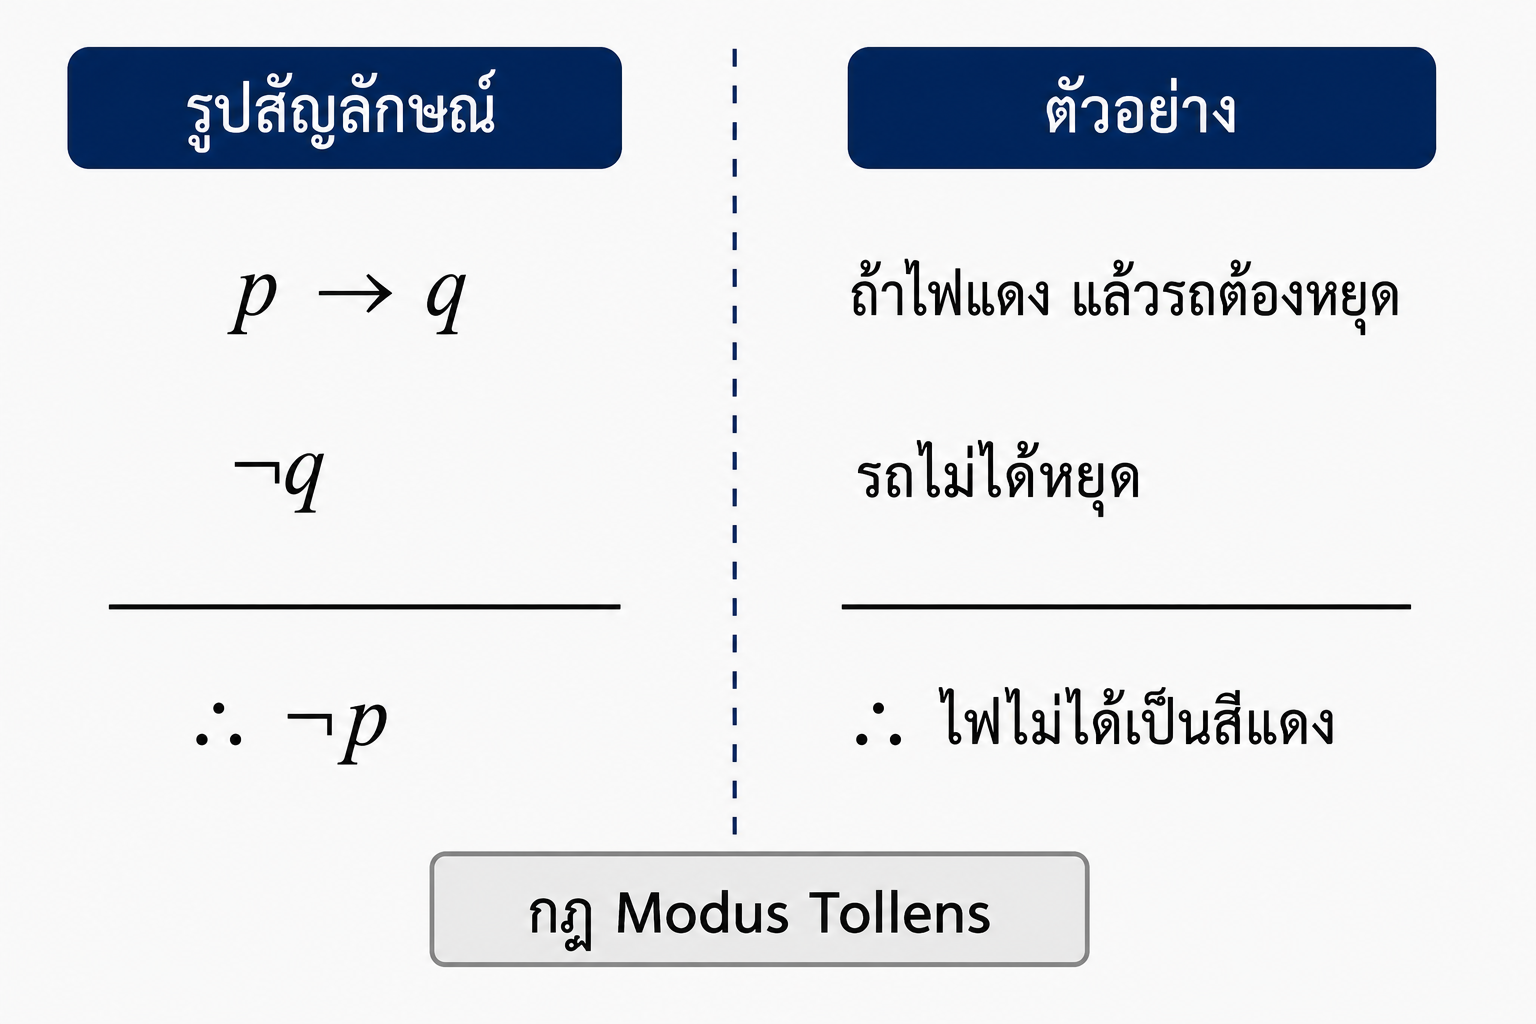
\includegraphics[width=0.85\textwidth]{Figures/08-modus-tollens.png}
    \caption{แผนผังแสดงกฎการอนุมานแบบ Modus Tollens}
    \label{fig:modus-tollens}
\end{figure}

รูปที่ \ref{fig:modus-tollens} แสดงโครงสร้างการอนุมานแบบ Modus Tollens (ละติน: \textit{Modus Tollendo Tollens} แปลว่า ``วิธีแห่งการปฏิเสธเพื่อสรุปผล'') ซึ่งใช้การปฏิเสธเงื่อนไขตามเพื่อสรุปปฏิเสธเงื่อนไขนำ

\subsubsection{โครงสร้างเชิงตรรกศาสตร์ของ Modus Tollens}
การอนุมานแบบ Modus Tollens ประกอบด้วยข้อตั้งต้น 2 ประพจน์ และข้อสรุป 1 ประพจน์
\begin{enumerate}
    \item ข้อตั้งต้นหลัก (Major Premise) คือประพจน์เงื่อนไข $p \rightarrow q$ (ถ้าเกิด $p$ แล้วจะเกิด $q$)
    \item ข้อตั้งต้นรอง (Minor Premise) คือประพจน์ปฏิเสธเงื่อนไขตาม $\neg q$ (ปรากฏว่า $q$ ไม่เกิดขึ้นจริง)
    \item ข้อสรุป (Conclusion) สามารถสรุปผลได้อย่างแน่ชัดว่าเงื่อนไขนำต้องไม่เกิดขึ้นจริง ($\therefore \neg p$)
\end{enumerate}

\subsubsection{การพิสูจน์ความสมเหตุสมผลด้วยตารางค่าความจริง (Tautology Proof)}
การอนุมานแบบ Modus Tollens มีความสมเหตุสมผลเนื่องจากรูปแบบประพจน์รวม
\begin{equation}
[(p \rightarrow q) \land \neg q] \rightarrow \neg p
\end{equation}
เป็น \textbf{สัจนิรันดร์ (Tautology)} ดังแสดงในตารางที่ \ref{tab:modus-tollens-valid}

\begin{table}[H]
    \centering
    \caption{ตารางค่าความจริงพิสูจน์ความสมเหตุสมผลของ Modus Tollens}
    \label{tab:modus-tollens-valid}
    \begin{tabular}{|c|c|c|c|c|c|c|}
        \hline
        $p$ & $q$ & $\neg p$ & $\neg q$ & $p \rightarrow q$ & $(p \rightarrow q) \land \neg q$ & $[(p \rightarrow q) \land \neg q] \rightarrow \neg p$ \\ \hline
        \textbf{T} & \textbf{T} & \textbf{F} & \textbf{F} & \textbf{T} & \textbf{F} & \textbf{T} \\ \hline
        \textbf{T} & \textbf{F} & \textbf{F} & \textbf{T} & \textbf{F} & \textbf{F} & \textbf{T} \\ \hline
        \textbf{F} & \textbf{T} & \textbf{T} & \textbf{F} & \textbf{T} & \textbf{F} & \textbf{T} \\ \hline
        \textbf{F} & \textbf{F} & \textbf{T} & \textbf{T} & \textbf{T} & \textbf{T} & \textbf{T} \\ \hline
    \end{tabular}
\end{table}

จากตารางที่ \ref{tab:modus-tollens-valid} จะเห็นว่าคอลัมน์สุดท้ายมีค่าความจริงเป็นจริง (T) ในทุกกรณี การอนุมานแบบ Modus Tollens จึงสมเหตุสมผล 100\%

\begin{ex}[การอนุมานแบบ Modus Tollens]
จงหาผลสรุปจากการให้เหตุผลต่อไปนี้ตามหลักเหตุผลทางตรรกศาสตร์
\begin{enumerate}
    \item ถ้าฝนตก แล้วพื้นถนนจะเปียก
    \item พื้นถนนไม่เปียก
\end{enumerate}
\end{ex}

\begin{solution}
กำหนด $p \equiv \text{ฝนตก}$, $q \equiv \text{พื้นถนนเปียก}$
\[
\begin{array}{r@{\quad}l}
\text{เหตุ 1} & p \rightarrow q\\
\text{เหตุ 2} & \neg q\\
\hline
\therefore & \neg p
\end{array}
\]
นั่นคือ $\neg p \equiv \text{ฝนไม่ตก}$ \solhere
\end{solution}

จากตัวอย่างจะเห็นว่า เมื่อทราบว่าถ้าฝนตกแล้วพื้นถนนจะเปียก และพื้นถนนไม่เปียก จึงสรุปได้ว่าฝนไม่ตก ทั้งนี้ต้องพิจารณาว่าอาจมีสาเหตุอื่นที่ทำให้พื้นเปียกได้ เช่น รดน้ำต้นไม้

\begin{ex}[การอนุมานแบบ Modus Tollens]
จงหาผลสรุปจากการให้เหตุผลต่อไปนี้ตามหลักเหตุผลทางตรรกศาสตร์
\begin{enumerate}
    \item ถ้าสัตว์เป็นสุนัข แล้วสัตว์นั้นเป็นสัตว์เลี้ยงลูกด้วยนม
    \item สัตว์ตัวนี้ไม่เป็นสัตว์เลี้ยงลูกด้วยนม
\end{enumerate}
\end{ex}

\begin{solution}
กำหนด $p \equiv \text{สัตว์เป็นสุนัข}$, $q \equiv \text{เป็นสัตว์เลี้ยงลูกด้วยนม}$
\[
\begin{array}{r@{\quad}l}
\text{เหตุ 1} & p \rightarrow q\\
\text{เหตุ 2} & \neg q\\
\hline
\therefore & \neg p
\end{array}
\]
นั่นคือ $\neg p \equiv \text{สัตว์ตัวนี้ไม่ใช่สุนัข}$ \solhere
\end{solution}

\subsubsection{การประยุกต์ใช้ในทางวิทยาการคอมพิวเตอร์และซอฟต์แวร์}
กฎ Modus Tollens มีบทบาทสำคัญในการทดสอบซอฟต์แวร์และการค้นหาข้อผิดพลาด (Debugging \& Fault Isolation) เช่น
\begin{itemize}
    \item \textbf{การทดสอบหน่วย (Unit Testing Verification)} หากกำหนดข้อตั้งต้นว่า ``ถ้าอัลกอริทึมทำงานถูกต้อง ($p$) แล้วจะได้ผลลัพธ์ $q$'' แต่เมื่อทดสอบ (Unit Test) พบว่าผลลัพธ์ที่ได้ไม่ใช่ $q$ ($\neg q$) นักพัฒนาสามารถสรุปด้วยกฎ Modus Tollens ได้ทันทีว่าอัลกอริทึมมีความผิดพลาดหรือมีบักเกิดขึ้น ($\neg p$)
    \item \textbf{การอนุมานย้อนกลับในระบบปัญญาประดิษฐ์ (Backward Chaining)} ในระบบสืบค้นและวินิจฉัยปัญหา (Diagnostic Expert Systems) กลไกจะใช้ Modus Tollens ในการตัดสาเหตุที่ไม่เกี่ยวข้องออก เมื่อผลลัพธ์อันไม่พึงประสงค์ไม่ได้เกิดขึ้น
\end{itemize}

\subsection{การอ้างเหตุผลแบบมีเงื่อนไข (Hypothetical Syllogism)}
\index{Hypothetical Syllogism}

Hypothetical Syllogism หรือ การอ้างเหตุผลแบบมีเงื่อนไข เป็นรูปแบบการอนุมานที่เชื่อมโยงเงื่อนไขหลายข้อเข้าด้วยกัน มีรูปแบบดังนี้

\begin{enumerate}
    \item ถ้า $p$ แล้ว $q$ โดยมีข้อตั้งต้นที่ 1
    \item ถ้า $q$ แล้ว $r$ และข้อตั้งต้นที่ 2
    \item $\therefore$ ถ้า $p$ แล้ว $r$ ผลสรุปคือ
\end{enumerate}

อ่านได้ว่า ถ้า $p$ นำไปสู่ $q$ และ $q$ นำไปสู่ $r$ แล้ว $p$ จะนำไปสู่ $r$ โดยตรง หลักการนี้เรียกว่า การถ่ายโอนเงื่อนไข (Conditional Transitivity) ซึ่งมีความสำคัญในการสร้างการให้เหตุผลที่ซับซ้อน

\begin{ex}[การอนุมานแบบ Hypothetical Syllogism]
จงหาผลสรุปจากการให้เหตุผลต่อไปนี้ตามหลักเหตุผลทางตรรกศาสตร์
\begin{enumerate}
    \item ถ้าฝนตก แล้วถนนจะเปียก
    \item ถ้าถนนเปียก แล้วรถจะลื่น
\end{enumerate}
\end{ex}

\begin{solution}
กำหนด $p \equiv \text{ฝนตก}$, $q \equiv \text{ถนนเปียก}$, $r \equiv \text{รถจะลื่น}$
\[
\begin{array}{r@{\quad}l}
\text{เหตุ 1} & p \rightarrow q\\
\text{เหตุ 2} & q \rightarrow r\\
\hline
\therefore & p \rightarrow r
\end{array}
\]
นั่นคือ $p \rightarrow r \equiv \text{ถ้าฝนตก แล้วรถจะลื่น}$ \solhere
\end{solution}

ตัวอย่างนี้แสดงให้เห็นว่าสามารถเชื่อมโยงเงื่อนไขหลายข้อเข้าด้วยกันเพื่อสร้างเงื่อนไขใหม่ที่ซับซ้อนขึ้น

ในการเขียนโปรแกรม Hypothetical Syllogism สามารถใช้ในการตรวจสอบเงื่อนไขแบบต่อเนื่อง เช่น ถ้า input ถูกต้อง แล้ว process จะทำงาน ถ้า process ทำงาน แล้ว output จะถูกสร้าง ดังนั้นถ้า input ถูกต้อง แล้ว output จะถูกสร้าง

\subsection{การอ้างเหตุผลแบบแยก (Disjunctive Syllogism)}
\index{Disjunctive Syllogism}

Disjunctive Syllogism หรือ การอ้างเหตุผลแบบแยก เป็นรูปแบบการอนุมานที่ใช้กับประพจน์ที่เชื่อมด้วย OR มีรูปแบบดังนี้

\begin{enumerate}
    \item $p \lor q$ โดยมีข้อตั้งต้นที่ 1
    \item $\neg p$ และข้อตั้งต้นที่ 2
    \item $\therefore q$ ผลสรุปคือ
\end{enumerate}

อ่านได้ว่า ถ้า $p$ หรือ $q$ เป็นจริง และ $p$ เป็นเท็จ แล้ว $q$ ต้องเป็นจริง หลักการคือเมื่อทราบว่าอย่างน้อยหนึ่งในสองอย่างเป็นจริง และทราบว่าอย่างหนึ่งเป็นเท็จ อีกอย่างหนึ่งต้องเป็นจริง

\begin{ex}[การอนุมานแบบ Disjunctive Syllogism]
จงหาผลสรุปจากการให้เหตุผลต่อไปนี้ตามหลักเหตุผลทางตรรกศาสตร์
\begin{enumerate}
    \item นาย ก อยู่บ้านหรืออยู่ที่ทำงาน
    \item นาย ก ไม่ได้อยู่ที่ทำงาน
\end{enumerate}
\end{ex}

\begin{solution}
กำหนด $p \equiv \text{นาย ก อยู่บ้าน}$, $q \equiv \text{นาย ก อยู่ที่ทำงาน}$
\[
\begin{array}{r@{\quad}l}
\text{เหตุ 1} & p \lor q\\
\text{เหตุ 2} & \neg q\\
\hline
\therefore & p
\end{array}
\]
นั่นคือ $p \equiv \text{นาย ก อยู่บ้าน}$ \solhere
\end{solution}

ในการเขียนโปรแกรม Disjunctive Syllogism สามารถใช้ในการตรวจสอบสถานะและการตัดสินใจ เช่น ถ้า error flag เป็น E1 หรือ E2 และตรวจพบว่า error flag ไม่ใช่ E1 แล้ว error flag ต้องเป็น E2

\section{การพิสูจน์ด้วยตารางค่าความจริง}
\index{การพิสูจน์!ตารางค่าความจริง}
\zlabel{sec:truth-table-proof}

\begin{ex}[การสร้างระบบการตัดสินใจ]
\label{ex:decision-tree-logic}
จงใช้ตรรกะประพจน์ในการสร้างระบบการตัดสินใจแบบง่าย (Decision Tree) สำหรับการอนุมัติสินเชื่อ โดยมีเงื่อนไขดังต่อไปนี้
\begin{enumerate}
    \item ถ้าผู้สมัครมีรายได้สูงกว่า 50,000 บาทต่อเดือน และไม่มีหนี้ค้างชำระ จะได้รับอนุมัติ
    \item ถ้าผู้สมัครมีรายได้สูงกว่า 50,000 บาทต่อเดือน แต่มีหนี้ค้างชำระ จะต้องพิจารณาเพิ่มเติม
    \item ถ้าผู้สมัครมีรายได้ต่ำกว่าหรือเท่ากับ 50,000 บาทต่อเดือน จะไม่ได้รับอนุมัติ
\end{enumerate}
จงเขียนประพจน์เชิงประกอบและตารางค่าความจริงสำหรับการตัดสินใจนี้
\end{ex}

\begin{solution}
กำหนดประพจน์
\begin{align*}
I &\equiv \text{ผู้สมัครมีรายได้สูงกว่า 50,000 บาทต่อเดือน}\\
D &\equiv \text{ผู้สมัครมีหนี้ค้างชำระ}\\
A &\equiv \text{ได้รับอนุมัติสินเชื่อ}\\
P &\equiv \text{ต้องพิจารณาเพิ่มเติม}\\
N &\equiv \text{ไม่ได้รับอนุมัติสินเชื่อ}
\end{align*}
จากเงื่อนไขทั้งสามเขียนประพจน์เชิงประกอบได้เป็น
\begin{align*}
A &\equiv I \land \neg D \quad (\text{เงื่อนไข 1})\\
P &\equiv I \land D \quad (\text{เงื่อนไข 2})\\
N &\equiv \neg I \quad (\text{เงื่อนไข 3})
\end{align*}

\begin{center}
\begin{tabular}{|c|c|c|c|c|c|}
\hline
$I$ & $D$ & $A$ & $P$ & $N$ & ผลการตัดสินใจ \\
\hline
\text{T} & \text{T} & \text{F} & \text{T} & \text{F} & พิจารณาเพิ่มเติม \\
\text{T} & \text{F} & \text{T} & \text{F} & \text{F} & อนุมัติ \\
\text{F} & \text{T} & \text{F} & \text{F} & \text{T} & ไม่อนุมัติ \\
\text{F} & \text{F} & \text{F} & \text{F} & \text{T} & ไม่อนุมัติ \\
\hline
\end{tabular}
\end{center}

จากตารางค่าความจริง ระบบจะอนุมัติเมื่อ $I \land \neg D$ เป็นจริง, พิจารณาเพิ่มเติมเมื่อ $I \land D$ และไม่อนุมัติเมื่อ $\neg I$ \solhere
\end{solution}

ในการวิเคราะห์ประพจน์เชิงประกอบที่ซับซ้อน การใช้ตารางค่าความจริงเป็นวิธีการที่เป็นระบบและแม่นยำในการตรวจสอบความสมมูลหรือความถูกต้องของประพจน์ การพิสูจน์ด้วยตารางค่าความจริงอาจใช้เวลานานหากประพจน์มีตัวแปรหลายตัว แต่ให้ผลลัพธ์ที่แน่นอนและตรวจสอบได้

การใช้ตารางค่าความจริงในการพิสูจน์มีหลายวัตถุประสงค์ ได้แก่ การตรวจสอบว่าประพจน์เป็นสัจนิรันดร์หรือไม่ การตรวจสอบว่าประพจน์สองประพจน์สมมูลกันหรือไม่ และการตรวจสอบความสมเหตุสมผลของการให้เหตุผล ในการพิสูจน์ว่าประพจน์สองประพจน์ $P$ และ $Q$ สมมูลกัน ($P \equiv Q$) จะต้องสร้างตารางค่าความจริงสำหรับทั้งสองประพจน์ แล้วเปรียบเทียบคอลัมน์ของผลลัพธ์ ถ้าค่าความจริงเหมือนกันทุกกรณี แสดงว่าประพจน์ทั้งสองสมมูลกัน

ในการพิสูจน์ว่าการให้เหตุผลสมเหตุสมผล โดยการเขียนข้อตั้งต้นทั้งหมดเชื่อมด้วย AND แล้วเชื่อมกับเงื่อนไขนำของผลสรุปด้วย $\rightarrow$ ถ้าประพจน์ที่ได้เป็นสัจนิรันดร์ แสดงว่าการให้เหตุผลนั้นสมเหตุสมผล

\begin{thrm}[ความสมมูลระหว่าง Implication กับ Disjunction]
\index{สมมูล!implication-disjunction}
สำหรับทุกประพจน์ $p$ และ $q$ จะได้ว่า
\begin{equation}
p \rightarrow q \equiv \neg p \lor q
\end{equation}
โดยที่ $p$ และ $q$ เป็นประพจน์ใดๆ, $\neg p$ คือนิเสธของ $p$ ที่กลับค่าความจริงจากจริงเป็นเท็จหรือจากเท็จเป็นจริง และ $\lor$ คือตัวเชื่อมแบบหรือที่จะเป็นจริงเมื่ออย่างน้อยหนึ่งประพจน์เป็นจริง นั่นคือประพจน์เชิงเงื่อนไขสมมูลกับการเชื่อมแบบหรือระหว่างนิเสธของเงื่อนไขนำกับเงื่อนไขตาม
\end{thrm}

\begin{proof}
\index{พิสูจน์!implication-disjunction}
พิจารณาตารางค่าความจริงสำหรับ $p \rightarrow q$ และ $\neg p \lor q$ ดังแสดงในตารางที่ \ref{tab:implies-equiv-proof}

สำหรับแถวที่ 1 เมื่อ $p = T$ และ $q = T$ จะได้ $p \rightarrow q = T$ และ $\neg p \lor q = F \lor T = T$ ค่าเท่ากัน

สำหรับแถวที่ 2 เมื่อ $p = T$ และ $q = F$ จะได้ $p \rightarrow q = F$ และ $\neg p \lor q = F \lor F = F$ ค่าเท่ากัน

สำหรับแถวที่ 3 เมื่อ $p = F$ และ $q = T$ จะได้ $p \rightarrow q = T$ และ $\neg p \lor q = T \lor T = T$ ค่าเท่ากัน

สำหรับแถวที่ 4 เมื่อ $p = F$ และ $q = F$ จะได้ $p \rightarrow q = T$ และ $\neg p \lor q = T \lor F = T$ ค่าเท่ากัน

เนื่องจากทั้ง 4 กรณีให้ค่าเท่ากันทุกแถว จึงสรุปได้ว่า $p \rightarrow q \equiv \neg p \lor q$ ตามที่ต้องการพิสูจน์
\end{proof}

ตัวอย่างการพิสูจน์ พิสูจน์ว่า $p \rightarrow q$ และ $\neg p \lor q$ มีค่าความจริงเหมือนกัน (สมมูลกัน)

\begin{table}[h]
    \centering
\caption{ตารางพิสูจน์ว่า $p \rightarrow q \equiv \neg p \lor q$}
\label{tab:implies-equiv-proof}
    \begin{tabular}{|c|c|c|c|c|c|}
        \hline
        \textbf{$p$} & \textbf{$q$} & \textbf{$p \rightarrow q$} & \textbf{$\neg p$} & \textbf{$\neg p \lor q$} & \textbf{การสมมูลกัน} \\ \hline
        T & T & T & F & T & \checkmark \\ \hline
        T & F & F & F & F & \checkmark \\ \hline
        F & T & T & T & T & \checkmark \\ \hline
        F & F & T & T & T & \checkmark \\ \hline
    \end{tabular}
\end{table}

ตารางที่ \ref{tab:implies-equiv-proof} แสดงให้เห็นว่าคอลัมน์ $p \rightarrow q$ และ $\neg p \lor q$ มีค่าเหมือนกันทุกแถว จึงสรุปได้ว่า $p \rightarrow q \equiv \neg p \lor q$

ผลลัพธ์นี้มีความสำคัญอย่างยิ่งในการแปลงประพจน์เชิงเงื่อนไขให้อยู่ในรูปแบบที่ใช้เฉพาะ AND, OR, NOT ซึ่งมีประโยชน์ในการออกแบบวงจรดิจิทัลและการเขียนโปรแกรม

\section{สรุป}
\index{สรุป}
\zlabel{sec:summary}

บทนี้ได้กล่าวถึงพื้นฐานของตรรกศาสตร์ (Logic) ซึ่งเป็นรากฐานสำคัญของวิทยาการคอมพิวเตอร์และคณิตศาสตร์เชิงคำนวณ เนื้อหาครอบคลุมหัวข้อสำคัญหลายประการ โดยเริ่มจากความหมายและความสำคัญของตรรกศาสตร์ที่มีบทบาทในการให้เหตุผลอย่างมีระบบ ต่อด้วยประพจน์ (Propositions) ซึ่งเป็นหน่วยพื้นฐานที่สุดของตรรกศาสตร์ที่สามารถระบุค่าความจริงได้ และตัวเชื่อมประพจน์ (Logical Connectives) ทั้ง 5 ตัว ได้แก่ นิเสธ ($\neg$) การเชื่อมแบบและ ($\land$) การเชื่อมแบบหรือ ($\lor$) การเชื่อมแบบถ้า...แล้ว ($\rightarrow$) และการเชื่อมแบบก็ต่อเมื่อ ($\leftrightarrow$) ตารางค่าความจริง (Truth Tables) เป็นเครื่องมือสำคัญในการวิเคราะห์ค่าความจริงของประพจน์เชิงประกอบ ช่วยให้สามารถตรวจสอบค่าความจริงของประพจน์ที่ซับซ้อนได้อย่างเป็นระบบ นอกจากนี้ยังได้ศึกษาประเภทของประพจน์เชิงประกอบ ได้แก่ สัจนิรันดร์ (Tautology) ซึ่งเป็นจริงทุกกรณี ข้อขัดแย้ง (Contradiction) ซึ่งเป็นเท็จทุกกรณี และประพจน์กลาง (Contingency) ซึ่งมีค่าความจริงขึ้นกับกรณี การอนุมาน (Inference Rules) เป็นกฎที่ใช้ในการสรุปผลอย่างมีตรรกะ ประกอบด้วย Modus Ponens, Modus Tollens, Hypothetical Syllogism และ Disjunctive Syllogism ซึ่งมีความสำคัญในการให้เหตุผลแบบนิรนัยและการเขียนโปรแกรม ทั้งหมดนี้เป็นพื้นฐานที่จำเป็นสำหรับการศึกษาบทต่อไปและการนำไปประยุกต์ใช้ในงานด้านวิทยาการคอมพิวเตอร์~\cite{rosen2019discrete}

\clearpage
\section{แบบฝึกหัดท้ายบท}

\begin{exercise}
จงพิจารณาว่าข้อความต่อไปนี้เป็นประพจน์หรือไม่ ถ้าเป็นให้ระบุค่าความจริง
\begin{enumerate}
    \item $3 + 5 = 8$
    \item $x > 10$
    \item กรุณาปิดประตู
    \item $7$ เป็นจำนวนคู่
    \item พรุ่งนี้จะเป็นวันพระ
    \item ความรักคือสิ่งสวยงาม
    \item $2^2 = 4$
\end{enumerate}
\end{exercise}

\begin{exercise}
จงสร้างตารางค่าความจริงของประพจน์ต่อไปนี้
\begin{enumerate}
    \item $p \land \neg q$
    \item $\neg p \lor q$
    \item $(p \rightarrow q) \land (q \rightarrow p)$
    \item $(p \lor q) \rightarrow r$
    \item $\neg(p \land q) \leftrightarrow (\neg p \lor \neg q)$
\end{enumerate}
\end{exercise}

\begin{exercise}
จงพิสูจน์ว่าประพจน์ต่อไปนี้เป็นสัจนิรันดร์หรือไม่ โดยใช้ตารางค่าความจริง
\begin{enumerate}
    \item $(p \rightarrow q) \lor (q \rightarrow p)$
    \item $(p \land q) \rightarrow p$
    \item $p \lor \neg p$
    \item $(p \rightarrow q) \leftrightarrow (\neg p \lor q)$
\end{enumerate}
\end{exercise}

\begin{exercise}
จงพิสูจน์ว่าประพจน์ต่อไปนี้เป็นข้อขัดแย้งหรือไม่
\begin{enumerate}
    \item $p \land \neg p$
    \item $\neg(p \lor \neg p)$
    \item $(p \rightarrow q) \land (p \land \neg q)$
\end{enumerate}
\end{exercise}

\begin{exercise}
จงใช้การอนุมานแบบ Modus Ponens หรือ Modus Tollens เพื่อหาผลสรุป
\begin{enumerate}
    \item ถ้าวันนี้ฝนตก แล้วฉันจะไม่ออกไปข้างนอก วันนี้ฝนตก $\therefore$ ?
    \item ถ้าข้าพเจ้าสอบผ่าน แล้วข้าพเจ้าจะดีใจ ข้าพเจ้าไม่ดีใจ $\therefore$ ?
    \item ถ้าผู้สมัครมีประสบการณ์ แล้วผู้สมัครจะได้รับการคัดเลือก ผู้สมัครไม่ได้รับการคัดเลือก $\therefore$ ?
\end{enumerate}
\end{exercise}

\begin{exercise}
จงตรวจสอบว่าประพจน์สมมูลกันหรือไม่
\begin{enumerate}
    \item $p \rightarrow q$ และ $\neg p \lor q$
    \item $\neg(p \land q)$ และ $\neg p \lor \neg q$ (กฎของ De Morgan ข้อที่ 1)
    \item $\neg(p \lor q)$ และ $\neg p \land \neg q$ (กฎของ De Morgan ข้อที่ 2)
    \item $p \leftrightarrow q$ และ $(p \rightarrow q) \land (q \rightarrow p)$
\end{enumerate}
\end{exercise}

\begin{exercise}
จงเขียนประพจน์ในรูปแบบเชิงสัญลักษณ์ โดยกำหนดให้ $p$ แทนฝนตก, $q$ แทนพื้นเปียก, และ $r$ แทนฉันจะอยู่บ้าน
\begin{enumerate}
    \item ถ้าฝนตก แล้วฉันจะอยู่บ้าน
    \item ฝนตกและพื้นเปียก
    \item ถ้าฝนไม่ตก แล้วฉันจะไม่อยู่บ้าน
    \item ฉันจะอยู่บ้านก็ต่อเมื่อฝนตกหรือพื้นเปียก
\end{enumerate}
\end{exercise}

\begin{exercise}
ให้นักศึกษาอธิบายความแตกต่างระหว่างสัจนิรันดร์ ข้อขัดแย้ง และประพจน์กลาง พร้อมยกตัวอย่างประกอบแต่ละประเภทอย่างน้อย 2 ตัวอย่าง
\end{exercise}

\clearpage
\section{เฉลยแบบฝึกหัด}
ในส่วนนี้แสดงเฉลยอย่างย่อสำหรับแบบฝึกหัดท้ายบทตามลำดับข้างต้น เพื่อให้ผู้เรียนใช้ตรวจคำตอบของตนเอง

\begin{enumerate}
    \item ระบุประพจน์และค่าความจริง (ก) เป็นประพจน์ ค่าจริง; (ข) ไม่เป็นประพจน์ เพราะมีตัวแปร $x$; (ค) ไม่เป็นประพจน์ เป็นประโยคคำสั่ง; (ง) เป็นประพจน์ ค่าเท็จ ($7$ เป็นจำนวนคี่); (จ) เป็นประโยคบอกเล่าเกี่ยวกับอนาคต ซึ่งในตรรกศาสตร์คลาสสิกมักถือว่าเป็นประพจน์ได้หากเหตุการณ์นั้นมีค่าความจริงแน่นอน แม้ผู้พูดจะยังไม่ทราบค่าความจริงในขณะกล่าว; (ฉ) ไม่เป็นประพจน์ เป็นข้อคิดเห็นเชิงค่านิยม; (ช) เป็นประพจน์ ค่าจริง
    \item ตารางค่าความจริง ใช้ $p,q,r \in \{T,F\}$ สร้างตารางขนาด $2^n$ แถว เช่น $p\land\neg q$ มีค่าจริงเฉพาะแถว $p=T, q=F$; $(p\rightarrow q)\land(q\rightarrow p)$ มีค่าจริงเมื่อ $p$ และ $q$ มีค่าตรงกัน (สมมูล $p\leftrightarrow q$)
    \item สัจนิรันดร์ (ก) เป็นสัจนิรันดร์ เพราะตรวจทุกแถวให้ค่าจริง; (ข) เป็นสัจนิรันดร์ (Law of Simplification); (ค) เป็นสัจนิรันดร์ (Law of Excluded Middle); (ง) เป็นสัจนิรันดร์ เพราะ $p\rightarrow q \equiv \neg p \lor q$
    \item ข้อขัดแย้ง (ก) เป็นข้อขัดแย้ง เพราะ $p\land\neg p$ เป็นเท็จเสมอ; (ข) เป็นข้อขัดแย้ง เพราะ $p\lor\neg p$ เป็นจริงเสมอ จึงนิเสธเป็นเท็จเสมอ; (ค) เป็นข้อขัดแย้ง เพราะถ้า $p\rightarrow q$ จริงและ $p$ จริง $q$ ต้องจริง ขัดกับ $\neg q$
    \item \textbf{Modus Ponens/Tollens:} (ก) สรุปว่า "ฉันจะไม่ออกไปข้างนอก" (Modus Ponens); (ข) สรุปว่า "ข้าพเจ้าสอบไม่ผ่าน" (Modus Tollens); (ค) สรุปว่า "ผู้สมัครไม่มีประสบการณ์" (Modus Tollens)
    \item ความสมมูล (ก) สมมูล โดยตารางค่าความจริง; (ข) และ (ค) สมมูล (กฎ De Morgan); (ง) สมมูล จากนิยามของไบคอนดิชันแนล
    \item ประพจน์เชิงสัญลักษณ์ (ก) $p\rightarrow r$; (ข) $p\land q$; (ค) $\neg p \rightarrow \neg r$; (ง) $r \leftrightarrow (p\lor q)$
    \item ความแตกต่าง สัจนิรันดร์คือประพจน์ที่จริงทุกการประเมิน (เช่น $p\lor\neg p$); ข้อขัดแย้งคือประพจน์ที่เท็จทุกการประเมิน (เช่น $p\land\neg p$); ประพจน์กลางคือมีทั้งจริงและเท็จ (เช่น $p\land q$, $p\rightarrow q$)
\end{enumerate}

\QAChapter
\begin{enumerate}
    \item จงระบุว่าข้อความต่อไปนี้เป็นประพจน์หรือไม่ พร้อมระบุค่าความจริงของข้อที่เป็นประพจน์ ดังนี้ (ก) กรุงเทพฯ เป็นเมืองหลวงของไทย (ข) $x + 3 = 10$ (ค) กรุณาปิดไฟ (ง) $3 \times 3 = 10$
    \item กำหนดให้ $p$ แทนฝนตก และ $q$ แทนถนนเปียก จงสร้างตารางค่าความจริงของ $p \rightarrow q$ และ $\neg p \lor q$ แล้วสรุปว่าทั้งสองประพจน์สมมูลกันหรือไม่
    \item จงพิสูจน์ด้วยตารางค่าความจริงว่า $(p \land q) \lor (p \land \neg q) \equiv p$
    \item จงจำแนกประพจน์ต่อไปนี้ว่าเป็นสัจนิรันดร์ ข้อขัดแย้ง หรือประพจน์กลาง (ก) $p \lor \neg p$ (ข) $p \land \neg p$ (ค) $(p \rightarrow q) \rightarrow (\neg q \rightarrow \neg p)$
    \item จงหา converse, inverse และ contrapositive ของประพจน์ "ถ้า $n$ หารด้วย 4 ลงตัว แล้ว $n$ หารด้วย 2 ลงตัว"
    \item จงใช้กฎ Modus Ponens สรุปผลจาก: ถ้าโปรแกรมไม่มีบัก แล้วโปรแกรมทำงานถูกต้อง, โปรแกรมไม่มีบัก
    \item จงตรวจสอบว่าการให้เหตุผลต่อไปนี้สมเหตุสมผลหรือไม่โดยใช้ตารางค่าความจริง จากสมมติฐาน $p \rightarrow q$ และ $\neg q$ สรุปได้ว่า $\neg p$
    \item จงประยุกต์ใช้ตรรกศาสตร์เขียนเงื่อนไขการรับสมัครงานต่อไปนี้เป็นสูตรตรรกศาสตร์ "ผู้สมัครต้องมีวุฒิปริญญาตรีและประสบการณ์ไม่น้อยกว่า 2 ปี หรือมีวุฒิปริญญาโท"
\end{enumerate}

\newpage
\sheetChapter{ตรรกศาสตร์ (Logic)}
\section*{วัตถุประสงค์}
\begin{enumerate}
    \item เพื่อให้ผู้เรียนอธิบายความหมายของประพจน์และค่าความจริงได้
    \item เพื่อให้ผู้เรียนสร้างและวิเคราะห์ตารางค่าความจริงสำหรับประพจน์เชิงประกอบได้
    \item เพื่อให้ผู้เรียนตรวจสอบความสมมูลทางตรรกศาสตร์และจำแนกประเภทของประพจน์ได้
    \item เพื่อให้ผู้เรียนประยุกต์ใช้กฎการอนุมานในการให้เหตุผลแบบนิรนัยได้
\end{enumerate}
\section*{คำชี้แจง} ให้ผู้เรียนศึกษาเนื้อหาบทตรรกศาสตร์ แล้วตอบคำถามต่อไปนี้
\begin{enumerate}
    \item จงอธิบายความแตกต่างระหว่างประพจน์เชิงเดี่ยวและประพจน์เชิงประกอบ พร้อมยกตัวอย่างอย่างละ 2 ข้อ
    \Pointilles{3}
    \item จงสร้างตารางค่าความจริงของ $p \rightarrow (q \lor \neg r)$ โดยใช้ตัวแปร $p$, $q$, $r$
    \Pointilles{3}
    \item จงพิสูจน์ว่า $p \leftrightarrow q \equiv (p \rightarrow q) \land (q \rightarrow p)$ ด้วยตารางค่าความจริง
    \Pointilles{3}
    \item จงอธิบายความหมายของ Modus Ponens และ Modus Tollens พร้อมยกตัวอย่างสถานการณ์จริงอย่างละ 1 ตัวอย่าง
    \Pointilles{3}
    \item จงตรวจสอบว่า $[(p \rightarrow q) \land (q \rightarrow r)] \rightarrow (p \rightarrow r)$ เป็นสัจนิรันดร์หรือไม่
    \Pointilles{3}
    \item จงอธิบายการเชื่อมโยงระหว่างตรรกศาสตร์กับการเขียนโปรแกรม พร้อมยกตัวอย่างการใช้ตัวเชื่อมตรรกะในคำสั่ง \texttt{if-else}
    \Pointilles{3}
\end{enumerate}

	\RefChapter
	
	%% บทที่ 2
	\cleartoleftpage
	\introChapter{ทฤษฎีเซต (Set Theory)}

\begin{description}[leftmargin=2cm, style=nextline, itemsep=0.1em, parsep=0pt]
    \item[รหัสวิชา] 4091606
    \item[ชื่อวิชา] คณิตศาสตร์สำหรับคอมพิวเตอร์
    \item[หน่วยกิต] 3 (3-0-6)
    \item[บทที่] 2
    \item[ชื่อบท] ทฤษฎีเซต (Set Theory)
    \item[จำนวนชั่วโมง] 6 ชั่วโมง
\end{description}

\noindent \textbf{\large วัตถุประสงค์การเรียนรู้ประจำบท}\par\vspace{0.2em}\noindent
\noindent เมื่อนักศึกษาเรียนบทนี้จบแล้ว นักศึกษาจะสามารถ
\begin{enumerate}[topsep=0.2em, itemsep=0.15em, leftmargin=*]
    \item อธิบายความหมายและสัญลักษณ์ของเซตได้
    \item ระบุประเภทของเซต เช่น เซตว่าง เซตจำกัด เซตอนันต์ได้
    \item ใช้การดำเนินการบนเซต เช่น ยูเนียน อินเตอร์เซกชัน ผลต่างเซต และคอมพลีเมนต์ได้
    \item พิสูจน์สมบัติของเซตโดยใช้แผนภาพเวนน์และพีชคณิตเซตได้
    \item ประยุกต์ใช้ทฤษฎีเซตในการแก้ปัญหาทางคอมพิวเตอร์ได้
\end{enumerate}

\noindent \textbf{\large หัวข้อที่สอน}\par\vspace{0.2em}\noindent
\begin{enumerate}[topsep=0.2em, itemsep=0.15em, leftmargin=*]
    \item นิยามและสัญลักษณ์ของเซต
    \item ความสัมพันธ์ระหว่างเซตและประเภทของเซต
    \item การดำเนินการระหว่างเซตและแผนภาพเวนน์
    \item กฎของเดมอร์แกน
    \item การนับจำนวนสมาชิกของเซต
    \item เซตที่นับได้และเซตที่นับไม่ได้
    \item การประยุกต์ทฤษฎีเซตในวิทยาการคอมพิวเตอร์
\end{enumerate}

\noindent \textbf{\large สื่อการสอน}
\begin{enumerate}[topsep=0.2em, itemsep=0.15em, leftmargin=*]
    \item สไลด์ประกอบการสอน
    \item แผนภาพเวนน์
    \item แบบฝึกหัดท้ายบท
\end{enumerate}

	\cleartoleftpage
	\chapter{ทฤษฎีเซต (Set Theory)}
\label{ch:set}

ทฤษฎีเซตใช้ระบุกลุ่มของวัตถุและความสัมพันธ์ระหว่างกลุ่มอย่างเป็นระบบ แนวคิดนี้ใช้กำหนดชนิดข้อมูล อธิบายการสืบค้นฐานข้อมูล และวิเคราะห์โครงสร้างทางคณิตศาสตร์ บทนี้อธิบายความเป็นมาของทฤษฎีเซต นิยามพื้นฐาน การดำเนินการระหว่างเซต และการประยุกต์ในวิทยาการคอมพิวเตอร์

\section{ความเป็นมาและความสำคัญของทฤษฎีเซต}
\label{sec:set-intro}
ทฤษฎีเซต (Set Theory) พัฒนาเป็นสาขาคณิตศาสตร์สมัยใหม่จากงานของแกออร์ก คันทอร์ (Georg Cantor, 1845--1918) นักคณิตศาสตร์ชาวเยอรมันในช่วงปลายศตวรรษที่ 19 งานของคันทอร์ศึกษาขนาดและชนิดของเซตอนันต์อย่างเป็นระบบ~\cite{halmos1974naive}

คันทอร์เริ่มศึกษาทฤษฎีเซตจากปัญหาเกี่ยวกับอนุกรมฟูเรียร์ (Fourier series) และความไม่ต่อเนื่องในการวิเคราะห์ทางคณิตศาสตร์ ทฤษฎีนี้ทำให้เปรียบเทียบขนาดของเซตอนันต์ได้ ตัวอย่างเช่น เซตของจำนวนเต็ม $\mathbb{Z}$ และเซตของจำนวนตรรกยะ $\mathbb{Q}$ เป็นเซตอนันต์นับได้ ขณะที่เซตของจำนวนจริง $\mathbb{R}$ เป็นเซตอนันต์นับไม่ได้ จึงมีขนาดมากกว่า

ปัจจุบันทฤษฎีเซตใช้เป็นภาษาสำหรับนิยามวัตถุ ความสัมพันธ์ และโครงสร้างในคณิตศาสตร์และวิทยาการคอมพิวเตอร์~\cite{halmos1974naive}

\subsection{ทฤษฎีเซตกับวิทยาการคอมพิวเตอร์}
แนวคิดของเซตปรากฏในชนิดข้อมูล การสืบค้นฐานข้อมูล และทฤษฎีภาษา การดำเนินการระหว่างเซตช่วยอธิบายการรวม การคัดเลือก และการเปรียบเทียบข้อมูล ตัวอย่างการนำไปใช้มีดังนี้~\cite{gersting2014structures}

\begin{enumerate}
    \item โครงสร้างข้อมูล อาร์เรย์และลิสต์เป็นลำดับข้อมูล จึงไม่ใช่เซตในความหมายทางคณิตศาสตร์ แต่ใช้เก็บตัวแทนของเซตได้เมื่อกำหนดวิธีจัดการข้อมูลซ้ำ ตารางแฮชใช้จับคู่คีย์กับตำแหน่งจัดเก็บ และโครงสร้างต้นไม้กับกราฟนิยามด้วยเซตของจุดยอดและความสัมพันธ์ระหว่างจุดยอด
    \item ระบบฐานข้อมูล ฐานข้อมูลเชิงสัมพันธ์มีพื้นฐานมาจากทฤษฎีเซตโดยตรง พีชคณิตเชิงสัมพันธ์ซึ่งเป็นพื้นฐานทางคณิตศาสตร์ของภาษาเอสคิวเอลประกอบด้วยการดำเนินการระหว่างเซต ได้แก่ ยูเนียน อินเตอร์เซกชัน ผลต่าง และผลคูณคาร์ทีเซียน
    \item ทฤษฎีภาษา ในการศึกษาภาษาการเขียนโปรแกรมและทฤษฎีการคำนวณ แนวคิดเรื่องตัวอักษร สายอักขระ และภาษา ล้วนอธิบายด้วยทฤษฎีเซต
    \item การตรวจสอบความถูกต้องของโปรแกรม การพิสูจน์ว่าโปรแกรมทำงานถูกต้องตามข้อกำหนดใช้การดำเนินการระหว่างเซตเพื่ออธิบายสถานะของโปรแกรม
    \item ทฤษฎีความน่าจะเป็น ปริภูมิตัวอย่างคือเซตของผลลัพธ์ที่เป็นไปได้ทั้งหมด และเหตุการณ์คือเซตย่อยของปริภูมิตัวอย่าง การดำเนินการระหว่างเหตุการณ์สอดคล้องกับการดำเนินการระหว่างเซต
    \item ตรรกศาสตร์และปัญญาประดิษฐ์ ระบบฐานความรู้ในปัญญาประดิษฐ์ใช้ทฤษฎีเซตในการจัดการข้อเท็จจริงและกฎเกณฑ์ การอนุมานสอดคล้องกับการดำเนินการระหว่างเซตของข้อเท็จจริง
\end{enumerate}

\begin{rem}
ในการเขียนโปรแกรม คำว่า ``เซตของตัวเลข'' อาจใช้เรียกข้อมูลในลิสต์หรืออาร์เรย์ที่มีข้อมูลซ้ำได้ แต่ในทางคณิตศาสตร์ เซตไม่มีสมาชิกซ้ำและไม่มีลำดับ เมื่อพิสูจน์สมบัติทางคณิตศาสตร์ ต้องใช้ความหมายของเซตตามนิยามนี้
\label{rem:set-programming}
\end{rem}


\section{นิยามพื้นฐานของเซต}
\label{sec:set-basics}

หัวข้อนี้อธิบายความหมายของเซต สมาชิก และวิธีเขียนเซต เนื้อหาเหล่านี้ใช้ในการนิยามการดำเนินการระหว่างเซต ความสัมพันธ์ระหว่างเซต และการพิสูจน์ทางเซตในหัวข้อถัดไป~\cite{enderton1977settheory}

ในทางคณิตศาสตร์ เซตคือกลุ่มของวัตถุที่กำหนดสมาชิกได้อย่างชัดเจน วัตถุที่อยู่ในกลุ่มเรียกว่า สมาชิก ตัวอย่างเช่น เซตของจำนวนเต็มบวกตั้งแต่ 1 ถึง 5 มีสมาชิกคือ 1, 2, 3, 4 และ 5

\subsection{นิยามของเซตและสมาชิก}
เมื่อเราจัดกลุ่มสิ่งต่าง ๆ เข้าด้วยกัน เราต้องมีวิธีบอกอย่างชัดเจนว่าสิ่งใด ``อยู่ในกลุ่ม'' หรือ ``ไม่อยู่ในกลุ่ม'' แนวคิดนี้นำไปสู่นิยามของเซตและสมาชิก ซึ่งเป็นพื้นฐานของทุกเรื่องในบทนี้ ข้อกำหนดสำคัญคือเงื่อนไขการเป็นสมาชิกต้องชัดเจนพอที่จะตัดสินได้ว่าสิ่งใดอยู่หรือไม่อยู่ในเซต โดยไม่ขึ้นกับความเห็นของผู้ตัดสิน เงื่อนไขนี้เป็นเหตุผลที่ข้อความอย่าง ``เซตของนักศึกษาที่เรียนเก่ง'' ไม่นับเป็นเซตในทางคณิตศาสตร์~\cite{lipschutz1998settheory}

\begin{definition}[เซตและสมาชิก]
\index{เซต!นิยาม}
\index{สมาชิก!นิยาม}
เซต คือกลุ่มของวัตถุที่มีสมบัติร่วมกันหรือระบุไว้อย่างชัดเจน โดยเรียกวัตถุแต่ละชิ้นว่า สมาชิก ของเซต ถ้า $a$ เป็นสมาชิกของเซต $A$ เขียนแทนด้วย $a \in A$ อ่านว่า ``$a$ เป็นสมาชิกของ $A$'' และถ้า $a$ ไม่เป็นสมาชิกของ $A$ เขียนแทนด้วย $a \notin A$
\label{def:set-membership}
\label{rem:epsilon-symbol}
\end{definition}

สัญลักษณ์ $\in$ มาจากอักษรกรีก epsilon ($\varepsilon$) ซึ่งคันทอร์นำมาใช้แทนความหมาย ``เป็นสมาชิกของ'' (element of) ข้อควรสังเกตคือความสัมพันธ์ $a \in A$ เป็นความสัมพันธ์ระหว่างวัตถุกับเซต ไม่ใช่ความสัมพันธ์ระหว่างเซตกับเซต~\cite{lipschutz1998settheory}

\begin{ex}[เซตในบริบทต่าง ๆ และสัญลักษณ์มาตรฐาน]
พิจารณาตัวอย่างต่อไปนี้ซึ่งแสดงเซตในบริบทที่แตกต่างกัน

\begin{enumerate}
    \item[(ก)] $A = \{1, 2, 3, 4, 5\}$. เซตนี้คือเซตของจำนวนเต็มบวกตั้งแต่ 1 ถึง 5 สมาชิกของ $A$ คือ 1, 2, 3, 4, 5 สังเกตว่าเราสามารถตรวจสอบได้ทันทีว่า $3 \in A$ เป็นจริง แต่ $7 \notin A$ ก็เป็นจริงเช่นกัน
    \item[(ข)] $B = \{\text{แดง}, \text{เขียว}, \text{น้ำเงิน}\}$. เซตนี้คือเซตของสีพื้นฐานในระบบสี RGB ลำดับไม่สำคัญ ดังนั้น $\{\text{แดง}, \text{เขียว}, \text{น้ำเงิน}\} = \{\text{เขียว}, \text{แดง}, \text{น้ำเงิน}\}$
    \item[(ค)] $\mathbb{N} = \{0, 1, 2, 3, \ldots\}$. เซตนี้คือเซตของจำนวนนับ (Natural Numbers) สัญลักษณ์ $\mathbb{N}$ เป็นมาตรฐาน ในตำราเล่มนี้เราจะถือว่า $\mathbb{N} = \{0, 1, 2, 3, \ldots\}$ โดยเริ่มที่ 0
    \item[(ง)] $\mathbb{Z} = \{\ldots, -2, -1, 0, 1, 2, \ldots\}$. เซตนี้คือเซตของจำนวนเต็ม (Integers) สัญลักษณ์ $\mathbb{Z}$ มาจากภาษาเยอรมัน ``Zahlen''
    \item[(จ)] $\mathbb{Q} = \left\{\frac{a}{b} \mid a, b \in \mathbb{Z}, b \neq 0\right\}$. เซตนี้คือเซตของจำนวนตรรกยะ (Rational Numbers) สัญลักษณ์ $\mathbb{Q}$ มาจาก ``quotient''
    \item[(ฉ)] $\mathbb{R}$ คือเซตของจำนวนจริง (Real Numbers) ซึ่งรวมจำนวนตรรกยะและจำนวนอตรรกยะ (irrational numbers) เช่น $\sqrt{2}$, $\pi$, $e$
\end{enumerate}
เมื่อเรากล่าวว่า $a \in A$ เรากำลังยืนยันว่าวัตถุ $a$ มีอยู่ในเซต $A$ ภายใต้การกำหนดเซตอย่างชัดเจน ข้อความนี้มีค่าความจริง (truth value) เป็นจริง (True) หรือเท็จ (False) อย่างใดอย่างหนึ่งเสมอ ไม่มีทางที่ $a \in A$ จะเป็น ``ครึ่งหนึ่งจริง'' หลักการนี้สัมพันธ์กับกฎทวิภาวะ (principle of bivalence) และสามารถเขียนในรูปกฎกีดกันกลางได้ว่า $(a \in A) \lor (a \notin A)$
\label{ex:set-examples}
\end{ex}

\begin{rem}
ความสัมพันธ์ระหว่างเซตของจำนวนต่าง ๆ เป็นดังนี้
\[
\mathbb{N} \subseteq \mathbb{Z} \subseteq \mathbb{Q} \subseteq \mathbb{R}
\]
จำนวนนับเป็นเซตย่อยของจำนวนเต็ม จำนวนเต็มเป็นเซตย่อยของจำนวนตรรกยะ และจำนวนตรรกยะเป็นเซตย่อยของจำนวนจริง ตัวอย่างเช่น $\frac{1}{2} \in \mathbb{Q}$ เป็นจริง และ $\frac{1}{2} \in \mathbb{R}$ ก็เป็นจริงด้วย แต่ $\sqrt{2} \notin \mathbb{Q}$ แต่ $\sqrt{2} \in \mathbb{R}$
\label{warn:number-sets}
\end{rem}

\begin{ex}[การตรวจสอบการเป็นสมาชิกของเซต]
จงพิจารณาว่าประโยคต่อไปนี้เป็นจริงหรือเท็จ พร้อมให้เหตุผลประกอบ
\begin{enumerate}
    \item $3 \in \{1, 2, 3, 4, 5\}$
    \item $7 \in \{1, 2, 3, 4, 5\}$
    \item $\sqrt{2} \in \mathbb{Q}$
    \item $\sqrt{2} \in \mathbb{R}$
    \item $0.75 \in \mathbb{Q}$
    \item $0.\overline{3} \in \mathbb{Q}$
\end{enumerate}
\end{ex}

\begin{solution}
\begin{align*}
3 \in \{1,2,3,4,5\} &\equiv \text{T}\\
7 \in \{1,2,3,4,5\} &\equiv \text{F}\\
\sqrt{2} \in \mathbb{Q} &\equiv \text{F} \quad (\sqrt{2} \text{ เป็นจำนวนอตรรกยะ})\\
\sqrt{2} \in \mathbb{R} &\equiv \text{T}\\
0.75 \in \mathbb{Q} &\equiv \text{T} \quad (0.75 = \tfrac{3}{4})\\
0.\overline{3} \in \mathbb{Q} &\equiv \text{T} \quad (0.\overline{3} = \tfrac{1}{3})
\end{align*}
\solhere
\end{solution}

\subsection{วิธีการเขียนเซต}
เซตเดียวกันสามารถเขียนแทนได้มากกว่าหนึ่งวิธี การเลือกวิธีเขียนขึ้นอยู่กับจำนวนสมาชิกและลักษณะของเซต ถ้าเซตมีสมาชิกไม่มากและระบุได้ครบทุกตัว การเขียนไล่สมาชิกออกมาโดยตรงจะชัดเจนที่สุด แต่ถ้าเซตมีสมาชิกจำนวนมากหรือมีจำนวนไม่สิ้นสุดจนไล่ไม่หมด เราจะอธิบายเซตด้วยเงื่อนไขที่สมาชิกทุกตัวต้องมีร่วมกันแทน ด้วยเหตุนี้ วิธีเขียนเซตที่ใช้กันจึงมี 2 แบบหลัก ดังนี้~\cite{rosen2019discrete}

\begin{enumerate}
    \item \textbf{แจกแจงสมาชิก (Roster Method)} คือการเขียนสมาชิกทั้งหมดภายในวงเล็บปีกกา $\{\}$ โดยคั่นด้วยเครื่องหมายจุลภาค วิธีนี้เหมาะกับเซตที่มีจำนวนสมาชิกน้อยและสามารถระบุได้ทั้งหมด

    \begin{enumerate}[leftmargin=2.5em,label=\arabic*.]
        \item $A = \{1, 2, 3\}$ แสดงเซตที่มีสมาชิกสามตัว $B = \{a, e, i, o, u\}$ แสดงเซตของสระในภาษาอังกฤษ สังเกตว่าลำดับไม่สำคัญ $\{a, e, i, o, u\} = \{e, a, i, o, u\}$ และไม่มีสมาชิกซ้ำ $\{1, 1, 2, 2, 3\} = \{1, 2, 3\}$
        \item \textbf{การใช้ ... (ellipsis):} เมื่อเซตมีสมาชิกมากแต่มีรูปแบบที่ชัดเจน เช่น $\{1, 2, 3, \ldots, 100\}$ แสดงเซตของจำนวนเต็มตั้งแต่ 1 ถึง 100 ข้อควรระวังคือต้องเขียนสมาชิกอย่างน้อย 2 ตัวก่อนจุดไข่ปลา เพื่อให้ผู้อ่านเข้าใจรูปแบบ
    \end{enumerate}

    \item \textbf{แจกแจงโดยกำหนดสมบัติ (Set-builder Notation)} คือการเขียนในรูป $\{x \mid \text{เงื่อนไขที่ } x \text{ ต้องสอดคล้อง}\}$ วิธีนี้เหมาะกับเซตที่มีจำนวนสมาชิกมากหรืออนันต์ พิจารณาตัวอย่างต่อไปนี้
    \begin{enumerate}[leftmargin=2.5em,label=\arabic*.]
        \item $A = \{x \in \mathbb{Z} \mid x > 0\}$. เซตนี้คือเซตของจำนวนเต็มบวก เขียนแบบย่อได้เป็น $\mathbb{Z}^+$
        \item $B = \{n^2 \mid n \in \mathbb{N} \text{ และ } n < 5\} = \{0, 1, 4, 9, 16\}$. สมาชิกของเซตนี้คือกำลังสองของจำนวนนับที่น้อยกว่า 5
        \item $E = \{x \in \mathbb{Z} \mid x \text{ หารด้วย } 2 \text{ ลงตัว}\} = 2\mathbb{Z}$. เซตนี้คือเซตของจำนวนคู่
        \item $O = \{x \in \mathbb{Z} \mid x \text{ หารด้วย } 2 \text{ ไม่ลงตัว}\}$. เซตนี้คือเซตของจำนวนคี่
        \item $C = \{x \in \mathbb{R} \mid x^2 - 5x + 6 = 0\} = \{2, 3\}$. เซตนี้คือเซตของคำตอบของสมการ $x^2 - 5x + 6 = 0$
        \item $D = \{x \in \mathbb{R} \mid x^2 + 1 = 0\} = \emptyset$. ไม่มีจำนวนจริงที่ยกกำลังสองแล้วบวก 1 ได้ศูนย์
    \end{enumerate}
\end{enumerate}

\begin{rem}
เซตมีสมบัติสำคัญสองประการดังนี้
\begin{enumerate}
    \item ไม่มีลำดับ (Unordered) คือลำดับของสมาชิกไม่สำคัญ $\{1, 2\} = \{2, 1\}$ หากต้องการลำดับ ต้องใช้ tuple หรือ sequence แทน
    \item ไม่มีสมาชิกซ้ำ (No Duplicates) คือ $\{1, 1, 2\} = \{1, 2\}$ หากต้องซ้ำ ต้องใช้ multiset หรือ list แทน
\end{enumerate}
\end{rem}


\subsection{เซตพิเศษ}
ในบรรดาเซตทั้งหมด มีบางเซตที่ปรากฏซ้ำ ๆ ในเกือบทุกหัวข้อจนคณิตศาสตร์กำหนดชื่อและสัญลักษณ์เฉพาะไว้ให้ การรู้จักเซตเหล่านี้ช่วยให้เขียนนิยามและพิสูจน์ได้กระชับและสื่อความตรงกัน หัวข้อนี้จะแนะนำเซตพิเศษที่ใช้บ่อยที่สุด ได้แก่ เซตว่างที่ไม่มีสมาชิกเลย เอกภพสัมพัทธ์ที่กำหนดขอบเขตของสิ่งที่พิจารณา และเซตของจำนวนมาตรฐานที่ใช้อ้างอิงตลอดทั้งเล่ม~\cite{epp2019discrete}

\begin{definition}[เซตพิเศษ]
\index{เซตพิเศษ!นิยาม}
เซตพิเศษที่ใช้บ่อย ได้แก่
\begin{enumerate}
    \item เซตว่าง เขียนแทนด้วย $\emptyset$ หรือ $\{\quad\}$ คือเซตที่ไม่มีสมาชิก
    \item เซตที่มีสมาชิกตัวเดียว คือเซตที่มีสมาชิกเพียงตัวเดียว เช่น $\{5\}$, $\{a\}$, $\{\emptyset\}$
    \item เอกภพสัมพัทธ์ เขียนแทนด้วย $U$ คือเซตของสมาชิกทั้งหมดที่พิจารณาในบริบทหนึ่ง
    \item เซตจำกัด คือเซตที่มีจำนวนสมาชิกจำกัด ส่วน เซตอนันต์ คือเซตที่มีจำนวนสมาชิกไม่สิ้นสุด เช่น $\mathbb{N}$, $\mathbb{Z}$, $\mathbb{Q}$, $\mathbb{R}$
\end{enumerate}
\label{def:special-sets}
\end{definition}

เซตว่างมีสมบัติที่ควรจำคือเป็นเซตย่อยของทุกเซต เขียนได้ว่า $\emptyset \subseteq A$ สำหรับทุกเซต $A$ เหตุผลคือข้อความ ``สมาชิกทุกตัวของ $\emptyset$ อยู่ใน $A$'' เป็นจริงโดยปริยาย (vacuous truth) เพราะ $\emptyset$ ไม่มีสมาชิกที่จะขัดกับเงื่อนไขได้ ส่วนเอกภพสัมพัทธ์ $U$ ทำหน้าที่เป็นกรอบกำหนดขอบเขตของสมาชิกที่นำมาพิจารณา การเลือก $U$ ต่างกันจะส่งผลต่อการดำเนินการบางอย่าง เช่น คอมพลีเมนต์ ดังจะเห็นในหัวข้อถัดไป

\begin{rem}[ข้อสังเกตเกี่ยวกับเซตว่าง]
\index{เซตว่าง!ข้อสังเกต}
ความเข้าใจผิดที่พบบ่อยเกี่ยวกับเซตว่างมีสองเรื่องดังนี้
\begin{enumerate}[label=\textbf{\arabic*.},leftmargin=1.5em,itemsep=0.3em]
    \item \textbf{ความแตกต่างของสัญลักษณ์:} $\emptyset$ คือเซตที่ไม่มีสมาชิกเลย ($|\emptyset| = 0$) แต่ $\{\emptyset\}$ คือเซตที่มีสมาชิก 1 ตัว คือ $\emptyset$ ($|\{\emptyset\}| = 1$) ดังนั้น $\emptyset \neq \{\emptyset\} \neq \{\{\emptyset\}\}$
    \item \textbf{ความแตกต่างระหว่างสมาชิกกับเซตย่อย:} $\emptyset \in \{\emptyset\}$ เป็นจริง เพราะ $\emptyset$ เป็นสมาชิกของ $\{\emptyset\}$ และ $\emptyset \subseteq \{\emptyset\}$ ก็เป็นจริงด้วย (เซตว่างเป็นเซตย่อยของทุกเซต) แสดงว่า $\in$ (เป็นสมาชิก) และ $\subseteq$ (เป็นเซตย่อย) เป็นความสัมพันธ์ที่ต่างกัน แต่สามารถเป็นจริงทั้งคู่พร้อมกันได้
\end{enumerate}
\end{rem}

\begin{ex}[การแยกความแตกต่างระหว่างการเป็นสมาชิกกับการเป็นเซตย่อย]
จงพิจารณาว่าข้อความต่อไปนี้เป็นจริงหรือเท็จ พร้อมให้เหตุผล
\begin{enumerate}
    \item $1 \in \{1, 2, 3\}$
    \item $\{1\} \in \{1, 2, 3\}$
    \item $\{1\} \subseteq \{1, 2, 3\}$
    \item $\emptyset \subseteq \{1, 2, 3\}$
    \item $\emptyset \in \{1, 2, 3\}$
\end{enumerate}
\end{ex}
\begin{solution}
\begin{align*}
1 \in \{1,2,3\} &\equiv \text{T} \quad (1 \text{ เป็นสมาชิก})\\
\{1\} \in \{1,2,3\} &\equiv \text{F} \quad (\{1\} \text{ ไม่ใช่สมาชิก})\\
\{1\} \subseteq \{1,2,3\} &\equiv \text{T} \quad (\text{ทุกสมาชิกของ } \{1\} \text{ อยู่ใน } \{1,2,3\})\\
\emptyset \subseteq \{1,2,3\} &\equiv \text{T} \quad (\text{เซตว่างเป็นเซตย่อยของทุกเซต})\\
\emptyset \in \{1,2,3\} &\equiv \text{F}
\end{align*}
หลักที่ใช้แยกสองความสัมพันธ์นี้คือ $\in$ เปรียบเทียบวัตถุกับเซต ส่วน $\subseteq$ เปรียบเทียบเซตกับเซต ข้อ 2 จึงเป็นเท็จ เพราะสมาชิกของ $\{1,2,3\}$ คือจำนวน 1, 2 และ 3 ไม่ใช่เซต $\{1\}$ ขณะที่ข้อ 3 เป็นจริงเพราะสมาชิกทุกตัวของ $\{1\}$ อยู่ใน $\{1,2,3\}$ ทั้งสองความสัมพันธ์เป็นจริงพร้อมกันได้ในบางกรณี เช่น $1 \in \{1\}$ และ $\{1\} \subseteq \{1\}$ \solhere
\end{solution}

\section{ความสัมพันธ์ระหว่างเซต}

เมื่อมีเซตสองเซต คำถามพื้นฐานที่ตามมาคือเซตทั้งสองเกี่ยวข้องกันอย่างไร สมาชิกของเซตหนึ่งอยู่ในอีกเซตหนึ่งครบทุกตัวหรือไม่ และเซตทั้งสองถือว่าเท่ากันเมื่อใด หัวข้อนี้ตอบคำถามเหล่านั้นด้วยแนวคิดเรื่องเซตย่อยและความเท่ากันของเซต ซึ่งเป็นเครื่องมือที่ใช้พิสูจน์ผลลัพธ์ทางทฤษฎีเซตแทบทุกข้อในหัวข้อถัดไป~\cite{johnsonbaugh2016discrete}

\subsection{เซตย่อย (Subset) และเซตย่อยแท้ (Proper Subset)}
นิยามเซตย่อยใช้เป็นพื้นฐานของการพิสูจน์ทางเซต เมื่อต้องการพิสูจน์ว่า $A \subseteq B$ ให้สมมติว่า $x \in A$ แล้วแสดงว่า $x \in B$ วิธีนี้เรียกว่าการพิสูจน์ตรง (Direct Proof) สำหรับเซตย่อย ส่วนเซตย่อยแท้เพิ่มเงื่อนไขว่าต้องมีสมาชิกใน $B$ อย่างน้อยหนึ่งตัวที่ไม่อยู่ใน $A$ การแยกสองแนวคิดนี้ทำให้ระบุได้ว่าเซตหนึ่งเท่ากับหรือเป็นเซตย่อยแท้ของอีกเซตหนึ่ง~\cite{halmos1974naive}

\begin{definition}[เซตย่อยและเซตย่อยแท้]
\index{เซตย่อย!นิยาม}
\index{เซตย่อยแท้!นิยาม}
เซต $A$ เป็นเซตย่อยของเซต $B$ เขียนแทนด้วย $A \subseteq B$ ก็ต่อเมื่อทุกสมาชิกของ $A$ เป็นสมาชิกของ $B$ กล่าวคือ $\forall x, (x \in A \rightarrow x \in B)$ นอกจากนี้ $\emptyset \subseteq A$ และ $A \subseteq A$ สำหรับทุกเซต $A$ เซต $A$ และ $B$ เท่ากันก็ต่อเมื่อ $A \subseteq B$ และ $B \subseteq A$ ส่วน $A \subseteq B$ และ $B \not\subseteq A$ หมายถึง $A \subsetneq B$ หรือ $A$ เป็นเซตย่อยแท้ของ $B$ ตัวอย่างเช่น $\{1, 2\} \subsetneq \{1, 2, 3\}$ เพราะ $\{1, 2\} \subseteq \{1, 2, 3\}$ แต่ $\{1, 2, 3\} \not\subseteq \{1, 2\}$
\end{definition}

\begin{ex}[การตรวจสอบความเป็นเซตย่อย]
จงพิจารณาว่าข้อความต่อไปนี้เป็นจริงหรือเท็จ พร้อมให้เหตุผล
\begin{enumerate}
    \item $\{1, 2\} \subseteq \{1, 2, 3\}$
    \item $\mathbb{N} \subseteq \mathbb{Z} \subseteq \mathbb{Q} \subseteq \mathbb{R}$
    \item $\emptyset \subseteq \{1, 2\}$
    \item $\{1, 2\} \not\subseteq \{2, 3\}$
\end{enumerate}
\end{ex}

\begin{solution}
ตรวจทีละข้อโดยไล่ดูว่าสมาชิกทุกตัวของเซตทางซ้ายอยู่ในเซตทางขวาหรือไม่
\begin{align*}
\{1,2\} \subseteq \{1,2,3\} &\equiv \text{T} \quad (1,2 \in \{1,2,3\})\\
\mathbb{N} \subseteq \mathbb{Z} \subseteq \mathbb{Q} \subseteq \mathbb{R} &\equiv \text{T}\\
\emptyset \subseteq \{1,2\} &\equiv \text{T} \quad (\text{เซตว่างเป็นเซตย่อยของทุกเซต})\\
\{1,2\} \not\subseteq \{2,3\} &\equiv \text{T} \quad (1 \in \{1,2\} \text{ แต่ } 1 \notin \{2,3\})
\end{align*}
ข้อ 4 ต้องอ่านให้ตรงว่าข้อความที่ถามคือ ``$\{1,2\}$ ไม่เป็นเซตย่อยของ $\{2,3\}$'' ซึ่งเป็นจริง เพราะพบสมาชิกอย่างน้อยหนึ่งตัวที่ขัดเงื่อนไข การหักล้างความเป็นเซตย่อยจึงต้องการตัวอย่างค้านเพียงตัวเดียวเท่านั้น \solhere
\end{solution}

\begin{principle}
ในการพิสูจน์ว่า $A = B$ เราต้องพิสูจน์ทั้ง $A \subseteq B$ และ $B \subseteq A$ นั่นคือต้องแสดงสองข้อ ข้อแรก ทุก $x \in A \Rightarrow x \in B$ (แสดง $A \subseteq B$) และข้อที่สอง ทุก $x \in B \Rightarrow x \in A$ ซึ่งแสดงว่า $B \subseteq A$ วิธีนี้เรียกว่าการพิสูจน์ด้วยการบรรจุสองทาง (double inclusion) เป็นเทคนิคมาตรฐานในการพิสูจน์ความเท่ากันของเซต
\label{thrm:double-inclusion}
\end{principle}

\begin{ex}[การพิสูจน์กฎการแจกแจงของเซต]
พิสูจน์ว่า $A \cap (B \cup C) = (A \cap B) \cup (A \cap C)$ (กฎการแจกแจง)
\end{ex}
\begin{solution}
พิสูจน์แบบสมาชิก โดยแสดงว่า $x$ อยู่ในเซตด้านซ้ายก็ต่อเมื่ออยู่ในเซตด้านขวา
\[
x \in A \cap (B \cup C) \Leftrightarrow x \in A \ \land\ (x \in B \lor x \in C)
\]
\[
\Leftrightarrow (x \in A \land x \in B) \lor (x \in A \land x \in C) \quad (\text{กฎแจกแจงตรรกศาสตร์})
\]
\[
\Leftrightarrow x \in (A \cap B) \ \lor\ x \in (A \cap C)
\]
\[
\Leftrightarrow x \in (A \cap B) \cup (A \cap C)
\]
$\therefore A \cap (B \cup C) = (A \cap B) \cup (A \cap C)$ \solhere
\end{solution}

\section{การดำเนินการระหว่างเซต (Set Operations)}

การดำเนินการระหว่างเซตเป็นเครื่องมือพื้นฐานในการสร้างเซตใหม่จากเซตที่มีอยู่ หัวข้อนี้ศึกษาการดำเนินการสี่อย่างหลัก ได้แก่ ยูเนียน ($\cup$) อินเตอร์เซกชัน ($\cap$) ผลต่าง ($-$) และคอมพลีเมนต์ ($^c$) การดำเนินการทั้งสี่มีคู่ขนานโดยตรงกับตัวเชื่อมทางตรรกศาสตร์ที่ศึกษาในบทที่ 1 คือ OR, AND, และ NOT ความสอดคล้องนี้ทำให้พิสูจน์สมบัติของเซตด้วยตารางค่าความจริงได้~\cite{enderton1977settheory}

\subsection{ยูเนียน (Union)}
ยูเนียนเป็นการรวมสมาชิกของสองเซตเป็นเซตเดียว สมาชิกที่อยู่ทั้งสองเซตปรากฏในผลลัพธ์เพียงครั้งเดียว เพราะเซตไม่นับสมาชิกซ้ำ ดังนั้นจำนวนสมาชิกของยูเนียนจึงไม่จำเป็นต้องเท่ากับผลบวกของจำนวนสมาชิกของทั้งสองเซต~\cite{lipschutz1998settheory}

\begin{definition}[ยูเนียน]
\index{ยูเนียน!นิยาม}
ยูเนียน ของเซต $A$ และ $B$ เขียนแทนด้วย $A \cup B$ คือเซตที่ประกอบด้วยสมาชิกที่อยู่ใน $A$ หรืออยู่ใน $B$ หรืออยู่ทั้งสองเซต นั่นคือ
\[ A \cup B = \{x \mid x \in A \text{ หรือ } x \in B\} \]
\label{def:union}
\end{definition}

สมาชิกจะเข้ามาอยู่ในผลลัพธ์ก็ต่อเมื่อมันอยู่ใน $A$ หรืออยู่ใน $B$ อย่างน้อยหนึ่งเซต และสมาชิกที่อยู่ทั้งสองเซตจะปรากฏในผลลัพธ์เพียงครั้งเดียว เพราะเซตไม่มีสมาชิกซ้ำ ยูเนียนมีสมบัติสำคัญดังนี้
\begin{enumerate}
    \item $A \cup A = A$ (กฎนิจพล)
    \item $A \cup \emptyset = A$ (กฎเอกลักษณ์)
    \item $A \cup U = U$ (กฎครอบงำ)
    \item $A \cup B = B \cup A$ (กฎการสลับที่)
    \item $(A \cup B) \cup C = A \cup (B \cup C)$ (กฎการเปลี่ยนหมู่)
\end{enumerate}
นอกจากนี้ยังได้ว่า $A \subseteq A \cup B$ และ $B \subseteq A \cup B$ สำหรับทุกเซต $A$, $B$, $C$

\begin{ex}[การหายูเนียนในกรณีต่าง ๆ]
จงหาผลของยูเนียนต่อไปนี้ พร้อมระบุสมบัติที่แต่ละข้อแสดงให้เห็น
\begin{enumerate}
    \item $\{1, 2\} \cup \{2, 3\}$
    \item $\{1, 2\} \cup \emptyset$
    \item $\{x \mid x \text{ เป็นจำนวนคู่}\} \cup \{x \mid x \text{ เป็นจำนวนคี่}\}$
    \item $A \cup A$ และ $A \cup B$ เทียบกับ $B \cup A$
\end{enumerate}
\end{ex}
\begin{solution}
\begin{align*}
\{1,2\} \cup \{2,3\} &= \{1,2,3\} \quad (2 \text{ อยู่ทั้งสองเซต ปรากฏครั้งเดียว})\\
\{1,2\} \cup \emptyset &= \{1,2\} \quad (\text{กฎเอกลักษณ์})\\
\{x \mid x \text{ คู่}\} \cup \{x \mid x \text{ คี่}\} &= \mathbb{Z}\\
A \cup A &= A \quad (\text{กฎนิจพล})\\
A \cup B &= B \cup A \quad (\text{กฎการสลับที่})
\end{align*}
\solhere
\end{solution}

\begin{ex}[การหายูเนียนของเซต]
กำหนดให้ $A = \{1, 2, 3, 4\}$ และ $B = \{3, 4, 5, 6\}$ จงหา $A \cup B$
\end{ex}

\begin{solution}
รวมสมาชิกที่อยู่ใน $A$ หรือ $B$ โดยนับสมาชิกที่ซ้ำเพียงครั้งเดียว
\begin{align*}
A \cup B &= \{1,2,3,4\} \cup \{3,4,5,6\}\\
         &= \{1,2,3,4,5,6\}
\end{align*}
สมาชิก 3 และ 4 อยู่ทั้งสองเซตแต่ปรากฏในผลลัพธ์เพียงครั้งเดียว ตามนิยามของเซตที่ไม่มีสมาชิกซ้ำ
\label{ex:union-step-by-step}
\solhere
\end{solution}

\begin{figure}[H]
    \centering
    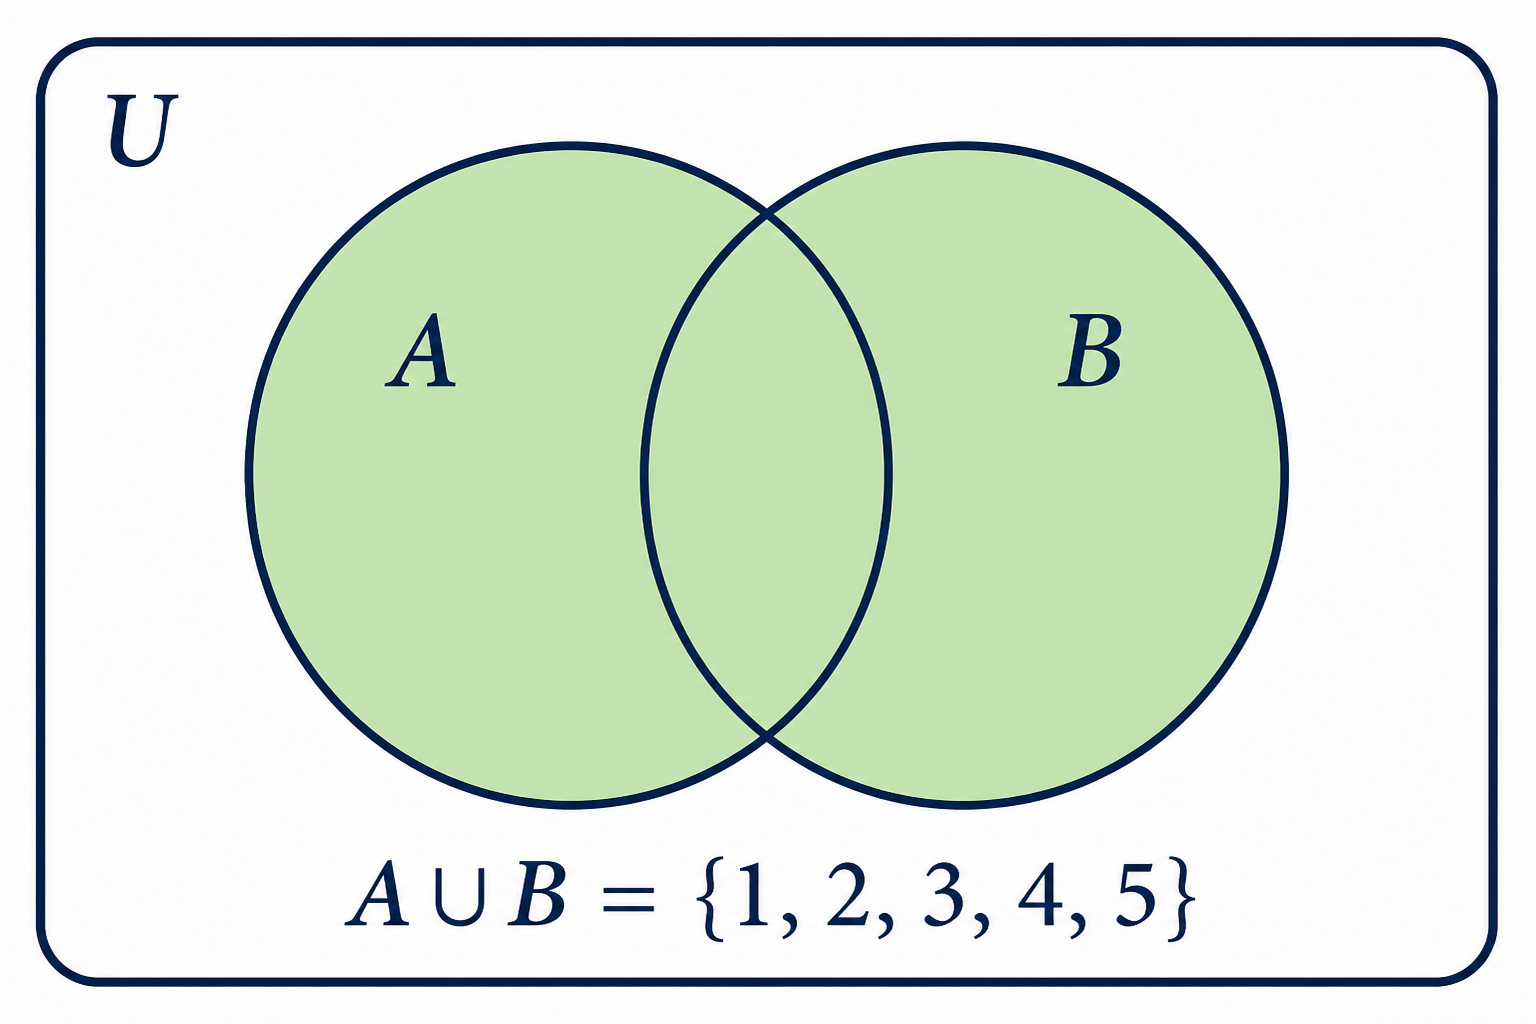
\includegraphics[width=0.65\textwidth]{Figures/png_ready/10-venn-union-generated.png}
    \caption{แผนภาพเวนน์แสดงการดำเนินการยูเนียน $A \cup B$}
    \label{fig:venn-union}
\end{figure}

รูปที่ \ref{fig:venn-union} แสดงแผนภาพเวนน์ของยูเนียน $A \cup B$ โดยพื้นที่ที่แรเงาคือผลลัพธ์ของการรวมเซต $A$ และเซต $B$

\subsection{อินเตอร์เซกชัน (Intersection)}
อินเตอร์เซกชัน (Intersection) คือเซตของสมาชิกที่อยู่ในทั้งสองเซต การที่ $x \in A \cap B$ หมายความว่า $x$ เป็นสมาชิกของ $A$ และเป็นสมาชิกของ $B$ ในทางตรรกศาสตร์สอดคล้องกับตัวเชื่อม ``และ'' (AND) ถ้า $A \cap B = \emptyset$ จะเรียก $A$ และ $B$ ว่า \textbf{เซตไม่มีสมาชิกร่วม (Disjoint Sets)}~\cite{rosen2019discrete}

\begin{definition}[อินเตอร์เซกชัน]
\index{อินเตอร์เซกชัน!นิยาม}
อินเตอร์เซกชัน ของเซต $A$ และ $B$ เขียนแทนด้วย $A \cap B$ คือเซตที่ประกอบด้วยสมาชิกที่อยู่ทั้งใน $A$ และใน $B$ พร้อมกัน นั่นคือ
\[ A \cap B = \{x \mid x \in A \text{ และ } x \in B\} \]
\end{definition}

อินเตอร์เซกชันมีสมบัติสำคัญดังนี้
\begin{enumerate}
    \item $A \cap A = A$ (กฎนิจพล)
    \item $A \cap \emptyset = \emptyset$ (กฎครอบงำ)
    \item $A \cap U = A$ (กฎเอกลักษณ์)
    \item $A \cap B = B \cap A$ (กฎการสลับที่)
    \item $(A \cap B) \cap C = A \cap (B \cap C)$ (กฎการเปลี่ยนหมู่)
\end{enumerate}
นอกจากนี้ยังได้ว่า $A \cap B \subseteq A$ และ $A \cap B \subseteq B$

\begin{ex}[การหาอินเตอร์เซกชันในกรณีต่าง ๆ]
จงหาผลของอินเตอร์เซกชันต่อไปนี้ พร้อมระบุว่าคู่ใดเป็นเซตไม่มีสมาชิกร่วม
\begin{enumerate}
    \item $\{1, 2\} \cap \{2, 3\}$
    \item $\{1, 2\} \cap \{3, 4\}$
    \item $\mathbb{Z} \cap \mathbb{R}$
    \item $\{x \mid x \text{ เป็นจำนวนคู่}\} \cap \{x \mid x \text{ เป็นจำนวนคี่}\}$
\end{enumerate}
\end{ex}
\begin{solution}
\begin{align*}
\{1,2\} \cap \{2,3\} &= \{2\} \quad (2 \text{ อยู่ทั้งสองเซต})\\
\{1,2\} \cap \{3,4\} &= \emptyset \quad (\text{เซตไม่มีสมาชิกร่วม})\\
\mathbb{Z} \cap \mathbb{R} &= \mathbb{Z} \quad (\mathbb{Z} \subseteq \mathbb{R})\\
\{x \mid x \text{ คู่}\} \cap \{x \mid x \text{ คี่}\} &= \emptyset
\end{align*}
\solhere
\end{solution}

\begin{figure}[H]
    \centering
    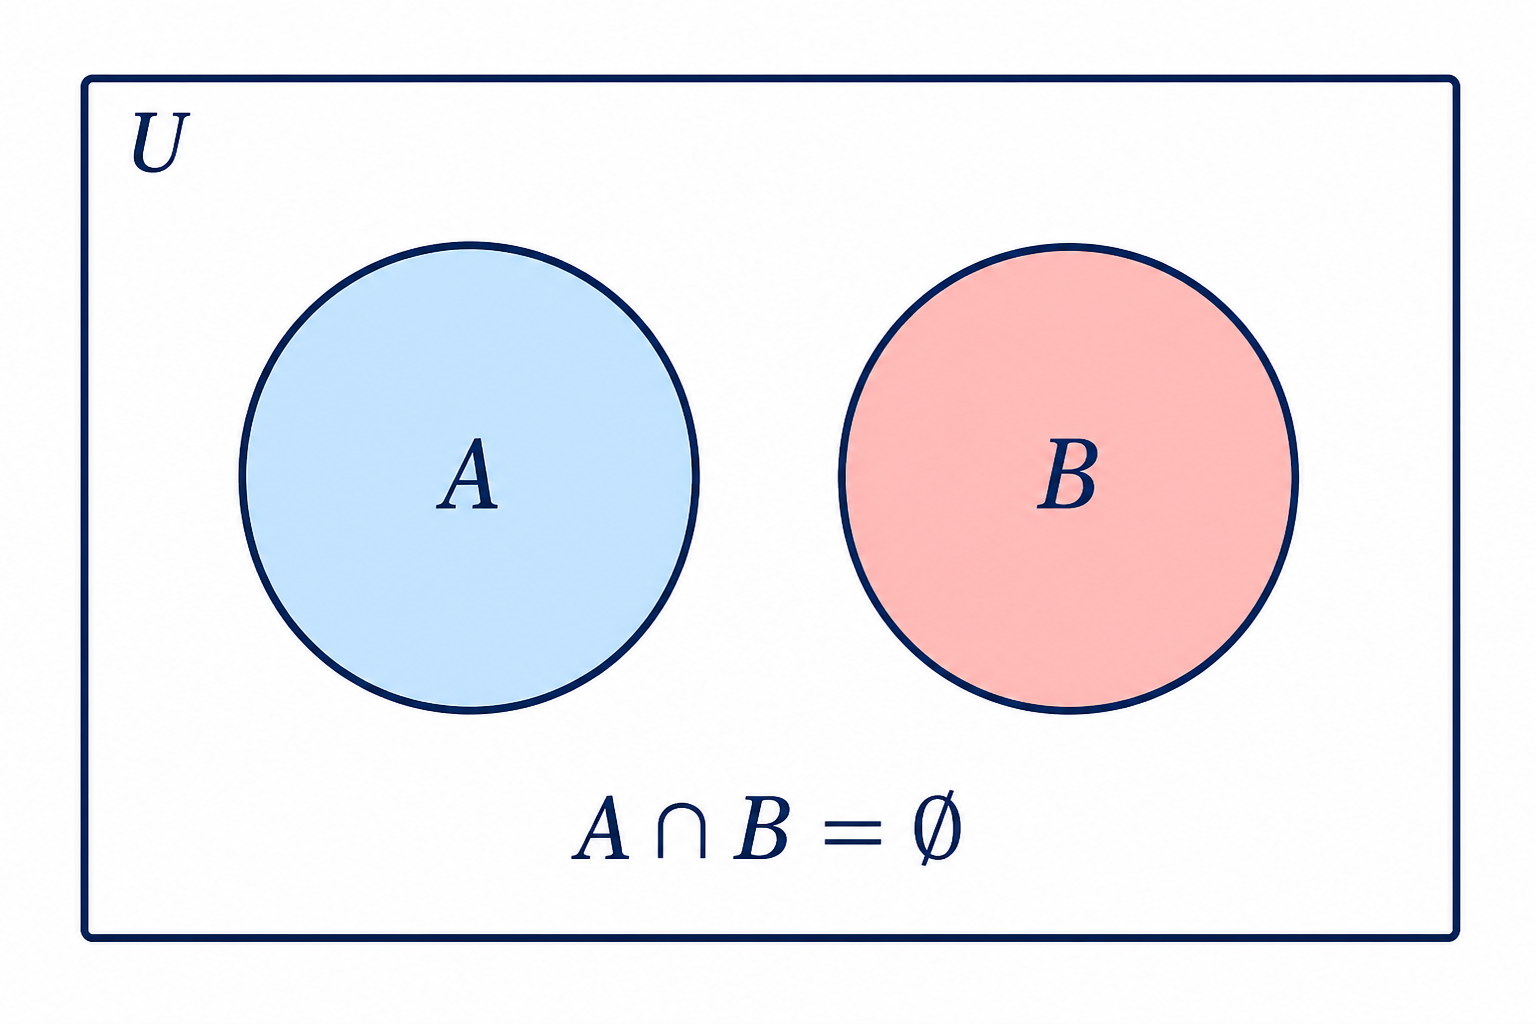
\includegraphics[width=0.62\textwidth]{Figures/png_ready/12-venn-disjoint-generated.png}
    \caption{แผนภาพแสดงเซตไม่มีสมาชิกร่วม เมื่อ $A\cap B=\emptyset$}
    \label{fig:venn-disjoint}
\end{figure}

กรณีพิเศษที่ควรสังเกตคือเมื่ออินเตอร์เซกชันเป็นเซตว่าง ดังรูปที่~\ref{fig:venn-disjoint} ซึ่งวงกลมสองวงไม่มีพื้นที่ทับซ้อนกันเลย เรียกเซตคู่นั้นว่าเซตไม่มีสมาชิกร่วม กรณีนี้ต่างจากรูปที่~\ref{fig:venn-intersection} ที่วงกลมทั้งสองมีพื้นที่ร่วมกัน ในทางปฏิบัติของงานข้อมูล เซตไม่มีสมาชิกร่วมหมายถึงเงื่อนไขสองข้อที่ไม่มีทางเป็นจริงพร้อมกัน เช่น รายการที่มีสถานะยกเลิกกับรายการที่มีสถานะชำระเงินแล้ว

\begin{ex}[การหาอินเตอร์เซกชันของเซต]
กำหนดให้ $A = \{2, 4, 6, 8, 10\}$ และ $B = \{3, 6, 9, 12\}$ จงหา $A \cap B$
\end{ex}

\begin{solution}
หาสมาชิกที่อยู่ทั้งใน $A$ และ $B$ พร้อมกัน
\begin{align*}
A \cap B &= \{2,4,6,8,10\} \cap \{3,6,9,12\}\\
         &= \{6\}
\end{align*}
มีเพียง 6 ที่อยู่ทั้งสองเซต สมาชิกตัวอื่นไม่เป็นสมาชิกร่วม (ถ้า $A \cap B = \emptyset$ จะเรียกว่าเซตไม่มีสมาชิกร่วม)
\label{ex:intersection-step-by-step}
\solhere
\end{solution}

\begin{figure}[H]
    \centering
    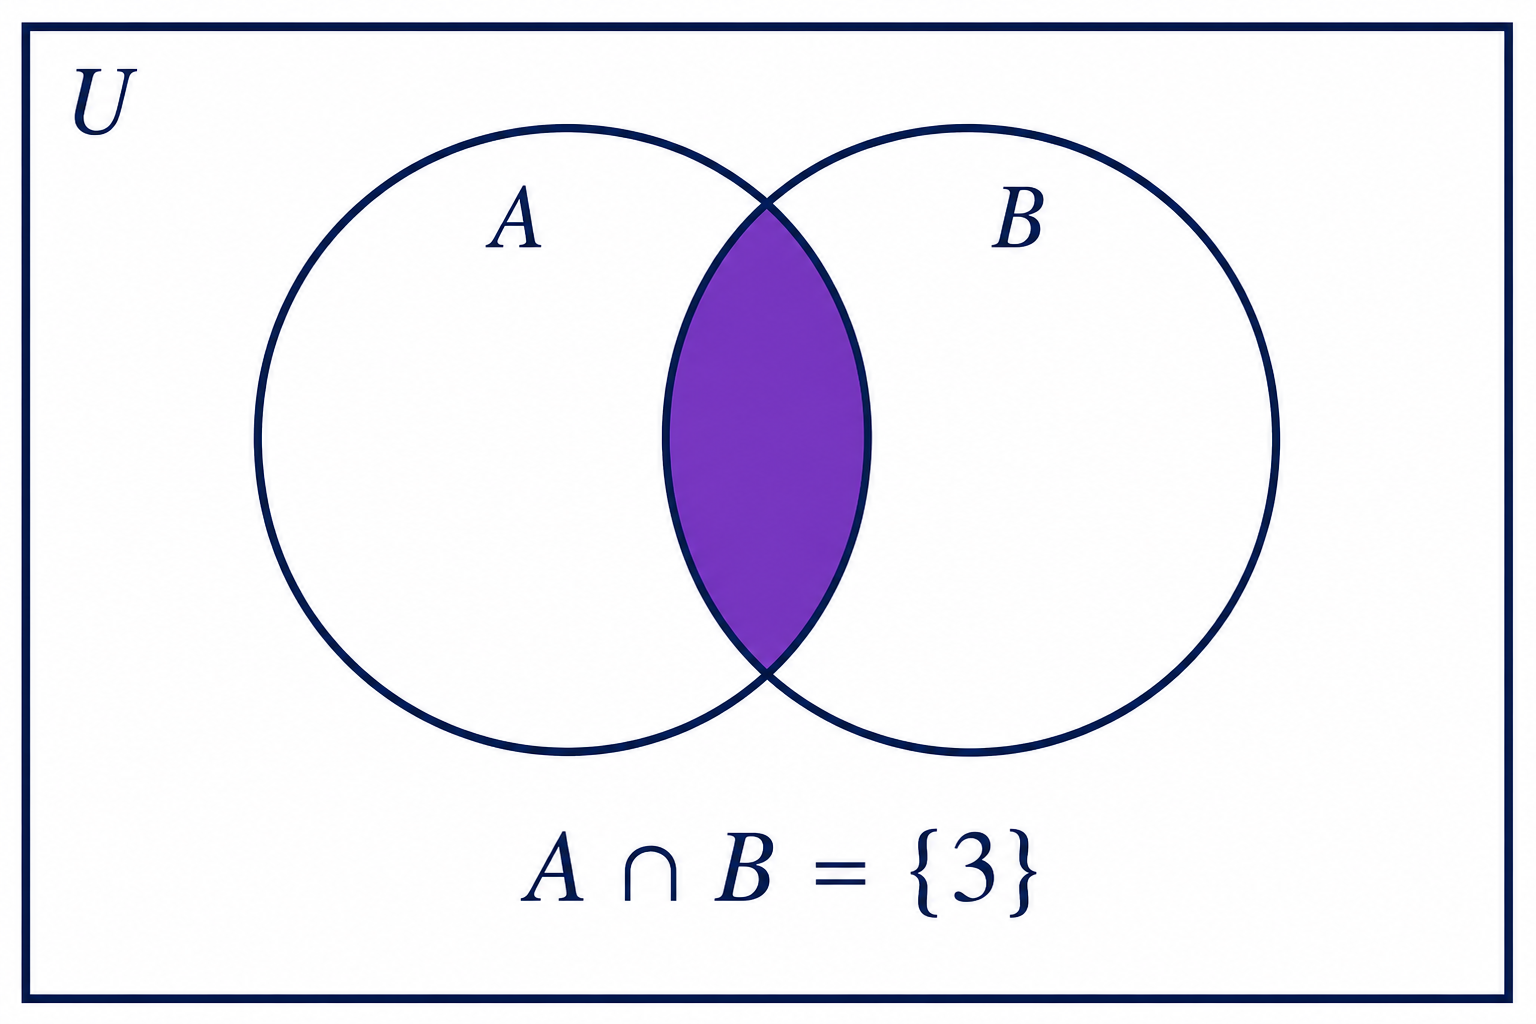
\includegraphics[width=0.65\textwidth]{Figures/png_ready/11-venn-intersection-generated.png}
    \caption{แผนภาพเวนน์แสดงการดำเนินการอินเตอร์เซกชัน $A \cap B$}
    \label{fig:venn-intersection}
\end{figure}

รูปที่ \ref{fig:venn-intersection} แสดงอินเตอร์เซกชัน $A \cap B$ โดยพื้นที่ที่แรเงาคือส่วนที่ทับซ้อนกันของเซต $A$ และเซต $B$ ซึ่งเป็นสมาชิกที่อยู่ทั้งสองเซต


\subsection{ผลต่าง (Set Difference)}
ผลต่างของเซตคือการนำสมาชิกของอีกเซตหนึ่งออกไป เหลือไว้เฉพาะสมาชิกที่อยู่ในเซตแรกแต่ไม่อยู่ในเซตที่สอง การดำเนินการนี้ไม่มีสมบัติสลับที่ กล่าวคือ $A - B$ กับ $B - A$ โดยทั่วไปให้ผลต่างกัน ต่างจากยูเนียนและอินเตอร์เซกชันที่สลับที่ได้ ในทางปฏิบัติผลต่างใช้แทนการคัดกรองข้อมูลออก เช่น การหารายชื่อผู้ที่ลงทะเบียนแล้วแต่ยังไม่ชำระเงิน~\cite{epp2019discrete}

\begin{definition}[ผลต่างระหว่างเซต]
\index{ผลต่างระหว่างเซต!นิยาม}
ผลต่าง ของเซต $A$ และ $B$ เขียนแทนด้วย $A - B$ คือเซตที่ประกอบด้วยสมาชิกที่อยู่ใน $A$ แต่ไม่อยู่ใน $B$ นั่นคือ
\[ A - B = \{x \mid x \in A \text{ และ } x \notin B\} \]
\label{def:set-difference}
\end{definition}

ในทางตรรกศาสตร์ผลต่างสอดคล้องกับ ``$A$ และไม่ $B$'' และโดยทั่วไป $A - B \neq B - A$ กล่าวคือผลต่างไม่มีสมบัติสลับที่ ตัวอย่างเช่น $\{1, 2\} - \{2, 3\} = \{1\}$ ในขณะที่ $\{2, 3\} - \{1, 2\} = \{3\}$

\begin{ex}[การหาผลต่างของเซต]
จงหาผลต่างของเซตต่อไปนี้
\begin{enumerate}
    \item $\{1, 2, 3\} - \{2, 4\}$
    \item $\mathbb{Z} - \mathbb{N}$
    \item $\{1, 2\} - \{1, 2\}$
    \item $\{1, 2\} - \{3, 4\}$
\end{enumerate}
\end{ex}
\begin{solution}
\begin{align*}
\{1,2,3\} - \{2,4\} &= \{1,3\} \quad (\text{นำ 2 ออก; 4 ไม่อยู่ในเซตแรก})\\
\mathbb{Z} - \mathbb{N} &= \{x \in \mathbb{Z} \mid x < 0\} = \mathbb{Z}^-\\
\{1,2\} - \{1,2\} &= \emptyset\\
\{1,2\} - \{3,4\} &= \{1,2\}
\end{align*}
\solhere
\end{solution}

\begin{rem}
ตัวอย่างการนำไปใช้ ให้ $U$ เป็นเซตของนักศึกษาทั้งหมด และ $A$ เป็นเซตของนักศึกษาที่สอบผ่าน แล้ว $U - A$ คือเซตของนักศึกษาที่สอบตก
\end{rem}

\begin{ex}[การหาผลต่างของเซต]
กำหนดให้ $A = \{a, b, c, d, e\}$ และ $B = \{b, d, f\}$ จงหา $A - B$
\end{ex}

\begin{solution}
หาสมาชิกที่อยู่ใน $A$ แต่ไม่อยู่ใน $B$
\begin{align*}
A - B &= \{a,b,c,d,e\} - \{b,d,f\}\\
      &= \{a,c,e\}
\end{align*}
$b$ และ $d$ ถูกนำออกเพราะอยู่ใน $B$; $f$ ไม่อยู่ใน $A$ จึงไม่กระทบผลลัพธ์ (โดยทั่วไป $A - B \neq B - A$)
\label{ex:difference-step-by-step}
\solhere
\end{solution}

\begin{figure}[H]
    \centering
    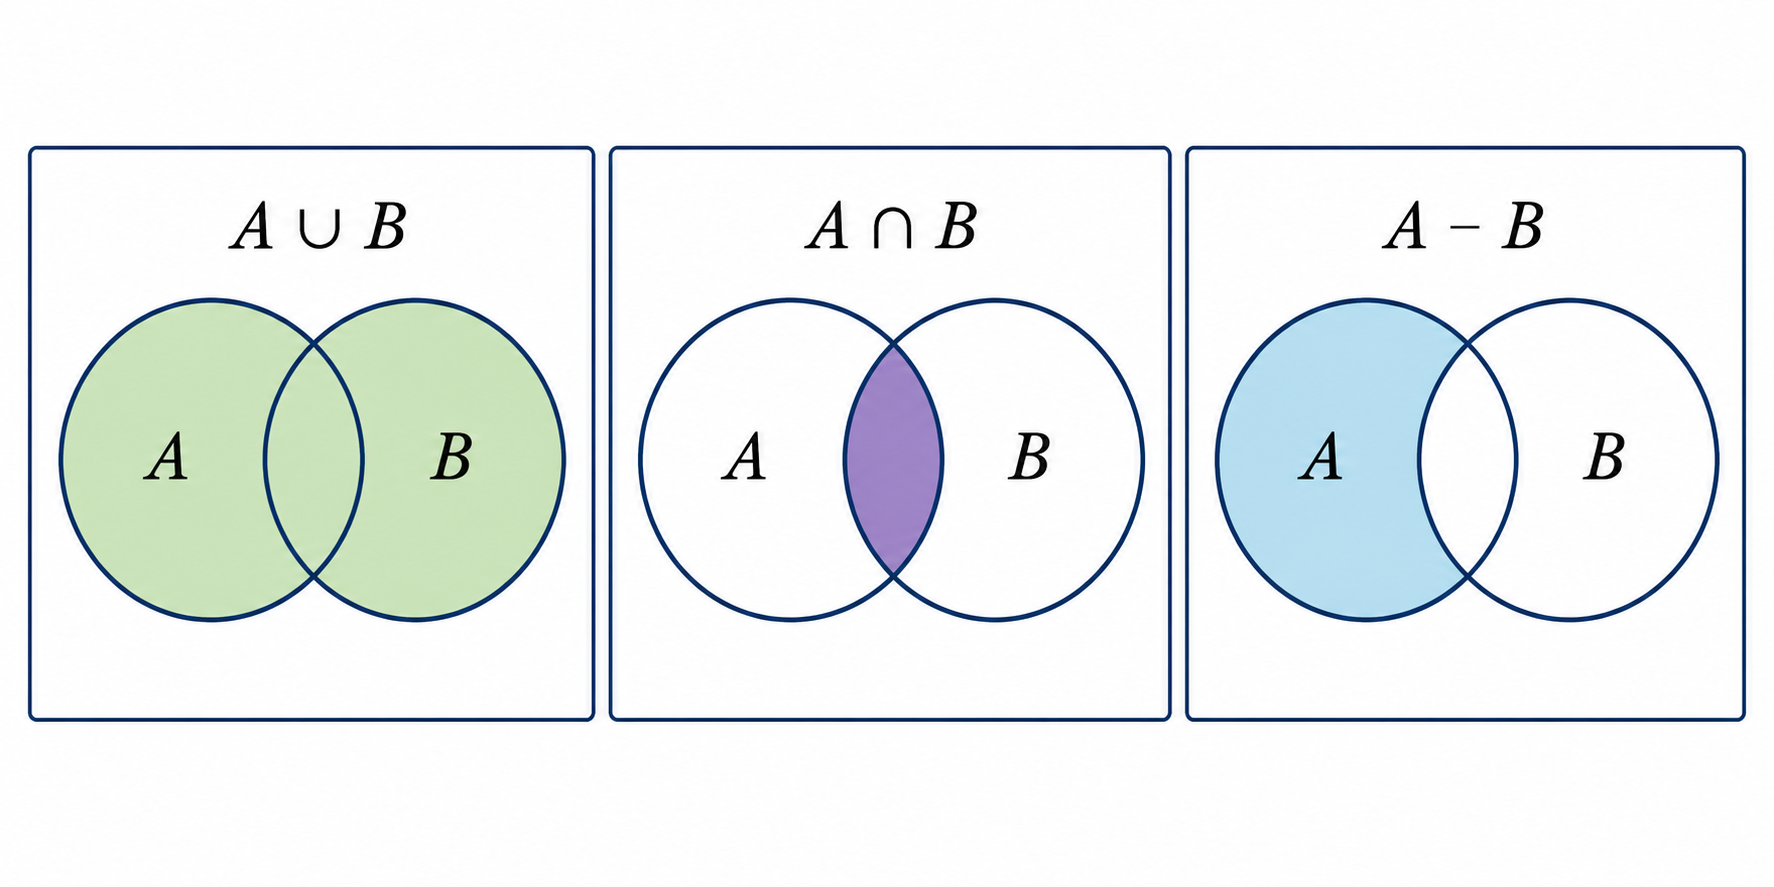
\includegraphics[width=0.90\textwidth]{Figures/png_ready/set-operations-generated.png}
    \caption{การแรเงาพื้นที่ของยูเนียน อินเตอร์เซกชัน และผลต่างของเซต}
    \label{fig:set-difference}
\end{figure}

รูปที่ \ref{fig:set-difference} เปรียบเทียบการแรเงาพื้นที่ของการดำเนินการหลักสามชนิด โดยแผนภาพด้านขวาสุดแสดงผลต่าง $A-B$ ซึ่งเลือกเฉพาะส่วนที่อยู่ใน $A$ แต่ไม่อยู่ใน $B$

\subsection{คอมพลีเมนต์ (Complement)}
คอมพลีเมนต์เป็นการดำเนินการที่ให้ ``สิ่งที่ไม่อยู่ใน $A$'' โดยอ้างอิงกับเอกภพสัมพัทธ์ $U$ สิ่งสำคัญคือต้องกำหนดเอกภพสัมพัทธ์ก่อนเสมอ เพราะคอมพลีเมนต์ขึ้นอยู่กับบริบท เซตเดียวกันจึงมีคอมพลีเมนต์ต่างกันเมื่อเปลี่ยนเอกภพสัมพัทธ์ ตัวอย่างเช่น คอมพลีเมนต์ของเซตจำนวนคู่เมื่อเอกภพสัมพัทธ์เป็นจำนวนเต็ม คือเซตจำนวนคี่ แต่เมื่อเอกภพสัมพัทธ์เป็นจำนวนจริง คอมพลีเมนต์จะรวมจำนวนที่ไม่ใช่จำนวนเต็มเข้าไปด้วย~\cite{johnsonbaugh2016discrete}

\begin{definition}[คอมพลีเมนต์]
\index{คอมพลีเมนต์!นิยาม}
คอมพลีเมนต์ ของเซต $A$ เขียนแทนด้วย $A^c$ หรือ $\overline{A}$ คือเซตที่ประกอบด้วยสมาชิกทั้งหมดในเอกภพสัมพัทธ์ $U$ ที่ไม่อยู่ใน $A$ นั่นคือ
\[ A^c = \{x \in U \mid x \notin A\} = U - A \]
\label{def:complement}
\end{definition}

คอมพลีเมนต์มีสมบัติสำคัญดังนี้
\begin{enumerate}
    \item $A \cup A^c = U$ (กฎคอมพลีเมนต์)
    \item $A \cap A^c = \emptyset$ (กฎการไม่ขัดแย้ง)
    \item $(A^c)^c = A$ (กฎคอมพลีเมนต์ซ้อน)
    \item $A - B = A \cap B^c$ (ผลต่างในรูปอินเตอร์เซกชันกับคอมพลีเมนต์)
\end{enumerate}
สมบัติข้อสุดท้ายมีประโยชน์มาก เพราะช่วยเปลี่ยนผลต่างให้อยู่ในรูปอินเตอร์เซกชันกับคอมพลีเมนต์ ทำให้นำกฎการแจกแจงมาใช้ต่อได้ พิสูจน์สมบัติข้อนี้ได้โดยไล่ตามนิยามของผลต่างและคอมพลีเมนต์ทีละขั้น
\begin{align*}
x \in A - B
&\Leftrightarrow x \in A \ \land\ x \notin B \quad (\text{นิยามของผลต่าง})\\
&\Leftrightarrow x \in A \ \land\ x \in B^c \quad (\text{นิยามของคอมพลีเมนต์})\\
&\Leftrightarrow x \in A \cap B^c \quad (\text{นิยามของอินเตอร์เซกชัน})
\end{align*}
จึงได้ว่า $A - B = A \cap B^c$ สำหรับทุกเซต $A$ และ $B$ ในเอกภพสัมพัทธ์เดียวกัน

ประเด็นที่ผู้เรียนมักมองข้ามคือคอมพลีเมนต์ไม่ได้ขึ้นกับเซต $A$ เพียงอย่างเดียว แต่ขึ้นกับเอกภพสัมพัทธ์ที่เลือกด้วย ตัวอย่างต่อไปนี้แสดงให้เห็นว่าเซต $A$ ชุดเดิมให้คอมพลีเมนต์คนละคำตอบเมื่อเปลี่ยนเอกภพสัมพัทธ์

\begin{ex}[ผลของการเปลี่ยนเอกภพสัมพัทธ์ต่อคอมพลีเมนต์]
กำหนดให้ $A = \{1, 2\}$ จงหา $A^c$ เมื่อกำหนดเอกภพสัมพัทธ์เป็น
\begin{enumerate}
    \item $U_1 = \{1, 2, 3, 4, 5\}$
    \item $U_2 = \{1, 2, 3, 4, 5, 6, 7\}$
\end{enumerate}
\end{ex}
\begin{solution}
คอมพลีเมนต์คือสมาชิกทั้งหมดในเอกภพสัมพัทธ์ที่ไม่อยู่ใน $A$ จึงคำนวณจาก $U - A$ ในแต่ละกรณี
\begin{align*}
A^c &= U_1 - A = \{1,2,3,4,5\} - \{1,2\} = \{3,4,5\}\\
A^c &= U_2 - A = \{1,2,3,4,5,6,7\} - \{1,2\} = \{3,4,5,6,7\}
\end{align*}
เซต $A$ เป็นชุดเดิมทั้งสองกรณี แต่คอมพลีเมนต์ต่างกันเพราะเอกภพสัมพัทธ์ต่างกัน ด้วยเหตุนี้การเขียน $A^c$ โดยไม่ระบุเอกภพสัมพัทธ์จึงไม่มีความหมายที่ชัดเจน ในทางปฏิบัติของงานข้อมูล เอกภพสัมพัทธ์คือขอบเขตของชุดข้อมูลที่กำลังพิจารณา การเปลี่ยนขอบเขตจากทั้งตารางเป็นเฉพาะแถวที่ผ่านการกรองย่อมเปลี่ยนผลของการหาส่วนที่เหลือไปด้วย \solhere
\end{solution}

\begin{ex}[การหาคอมพลีเมนต์ของเซต]
กำหนดให้ $U = \{1, 2, 3, 4, 5, 6, 7, 8\}$ และ $A = \{2, 4, 6, 8\}$ จงหา $A^c$
\end{ex}

\begin{solution}
หาสมาชิกใน $U$ ที่ไม่อยู่ใน $A$
\begin{align*}
A^c &= U - A = \{1,2,3,4,5,6,7,8\} - \{2,4,6,8\}\\
    &= \{1,3,5,7\}
\end{align*}
จำนวนคู่ทั้งหมดอยู่ใน $A$ จึงไม่อยู่ใน $A^c$; จำนวนคี่ทั้งหมดอยู่ใน $A^c$ และตรวจได้ว่า $A \cup A^c = U$
\label{ex:complement-step-by-step}
\solhere
\end{solution}

\begin{figure}[H]
    \centering
    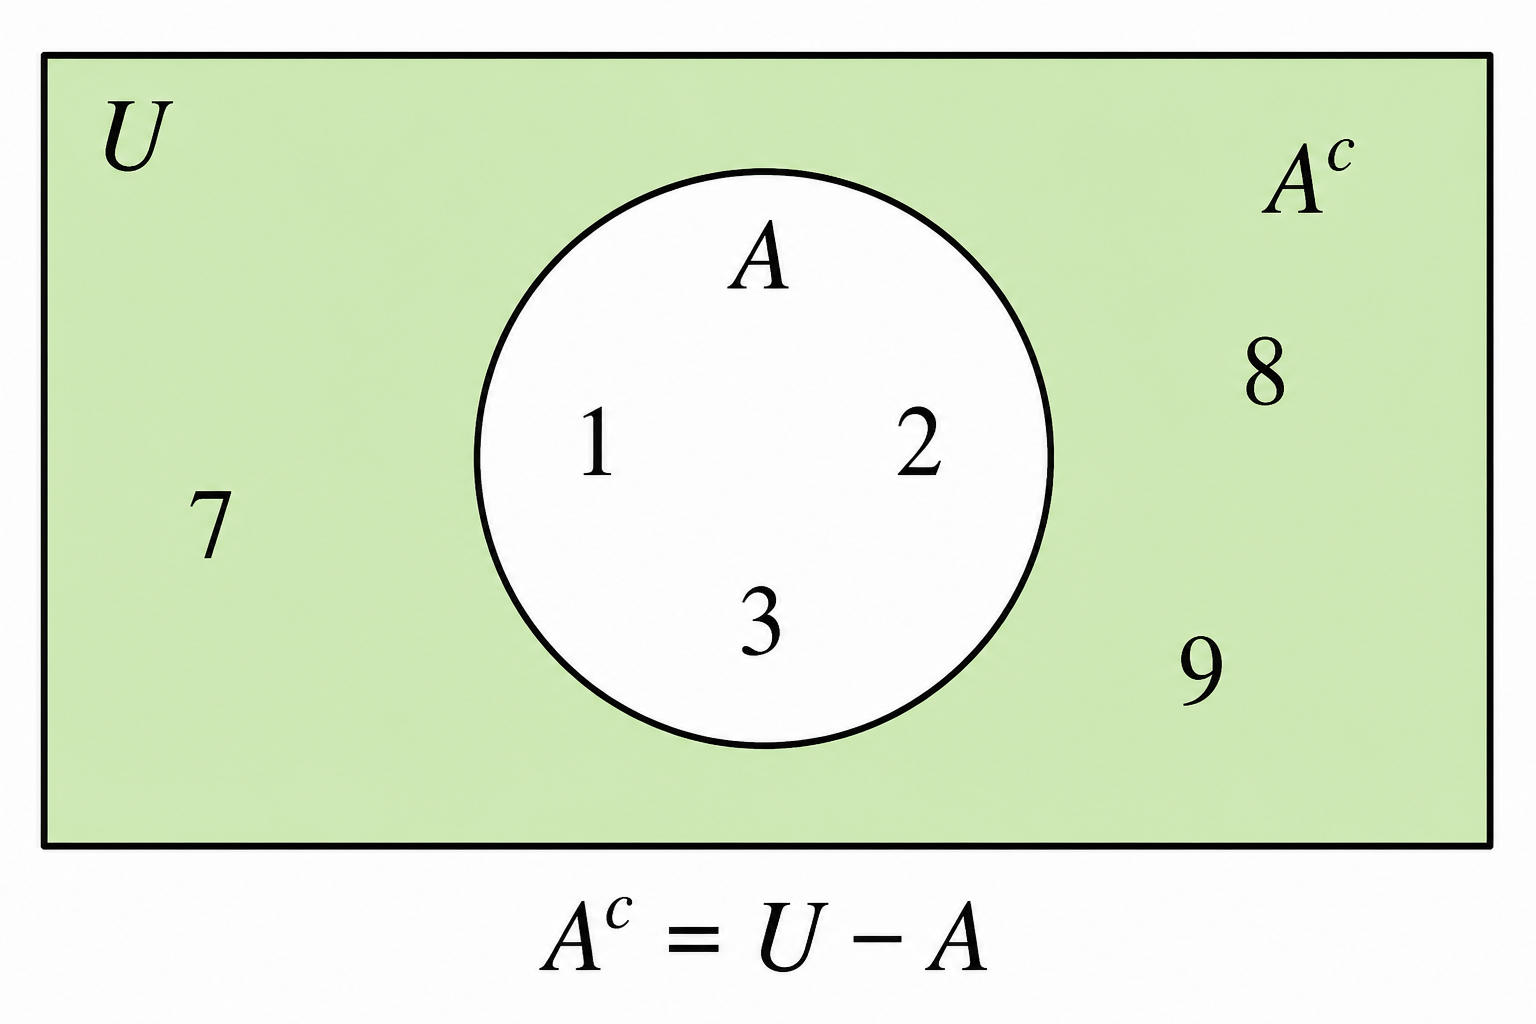
\includegraphics[width=0.65\textwidth]{Figures/png_ready/14-venn-complement-generated.png}
    \caption{แผนภาพเวนน์แสดงคอมพลีเมนต์ $A^c$ ของเซต $A$}
    \label{fig:venn-complement}
\end{figure}

รูปที่ \ref{fig:venn-complement} แสดงคอมพลีเมนต์ $A^c$ ซึ่งคือพื้นที่ทั้งหมดในเอกภพสัมพัทธ์ $U$ ที่ไม่อยู่ในเซต $A$ พื้นที่ที่แรเงาคือ $A^c$

เมื่อศึกษาการดำเนินการครบทั้งสี่ชนิดแล้ว จะพบว่าการดำเนินการเหล่านี้ไม่ได้เป็นอิสระต่อกัน แต่มีสมบัติร่วมกันเป็นชุดที่ใช้จัดรูปนิพจน์ของเซตได้ เช่นเดียวกับที่การบวกและการคูณของจำนวนจริงมีสมบัติการสลับที่และการเปลี่ยนหมู่ สมบัติชุดนี้เรียกรวมว่ากฎพีชคณิตของเซต และเป็นกฎชุดเดียวกับกฎพีชคณิตของประพจน์ใน\autoref{ch:logic} โดยเปลี่ยนจากตัวเชื่อมทางตรรกศาสตร์มาเป็นการดำเนินการระหว่างเซต

\begin{law}[กฎพีชคณิตของการดำเนินการกับเซต (Algebraic Laws for Set Operations)]
สำหรับเซต $A, B, C$ ใดๆ ในเอกภพสัมพัทธ์ $U$ การดำเนินการระหว่างเซตมีสมบัติดังต่อไปนี้

\begin{enumerate}
    \item กฎนิจพล (Idempotent Laws) $A \cup A = A$ และ $A \cap A = A$
    \item กฎเอกลักษณ์ (Identity Laws) $A \cup \emptyset = A$ และ $A \cap U = A$
    \item กฎครอบงำ (Domination Laws) $A \cup U = U$ และ $A \cap \emptyset = \emptyset$
    \item กฎการสลับที่ (Commutative Laws) $A \cup B = B \cup A$ และ $A \cap B = B \cap A$
    \item กฎการเปลี่ยนหมู่ (Associative Laws) $(A \cup B) \cup C = A \cup (B \cup C)$ และ $(A \cap B) \cap C = A \cap (B \cap C)$
    \item กฎการแจกแจง (Distributive Laws) $A \cap (B \cup C) = (A \cap B) \cup (A \cap C)$ และ $A \cup (B \cap C) = (A \cup B) \cap (A \cup C)$
    \item กฎการดูดกลืน (Absorption Laws) $A \cup (A \cap B) = A$ และ $A \cap (A \cup B) = A$
    \item กฎคอมพลีเมนต์ (Complement Laws) $A \cup A^c = U$, $A \cap A^c = \emptyset$, $(A^c)^c = A$, $\emptyset^c = U$, และ $U^c = \emptyset$
\end{enumerate}
\label{thrm:set-algebraic-laws}
\end{law}

\begin{ex}[การพิสูจน์กฎการดูดกลืน]
จงพิสูจน์กฎการดูดกลืน $A \cup (A \cap B) = A$ โดยใช้การพิสูจน์แบบสมาชิก
\label{ex:absorption-proof}
\end{ex}
\begin{solution}
พิสูจน์แบบสมาชิก
\begin{align*}
x \in A \cup (A \cap B)
&\Leftrightarrow x \in A \ \lor\ (x \in A \land x \in B)\\
&\Leftrightarrow x \in A \quad (\text{กฎการดูดกลืนของตรรกศาสตร์})
\end{align*}
$\therefore A \cup (A \cap B) = A$ \solhere
\end{solution}

\begin{figure}[H]
    \centering
    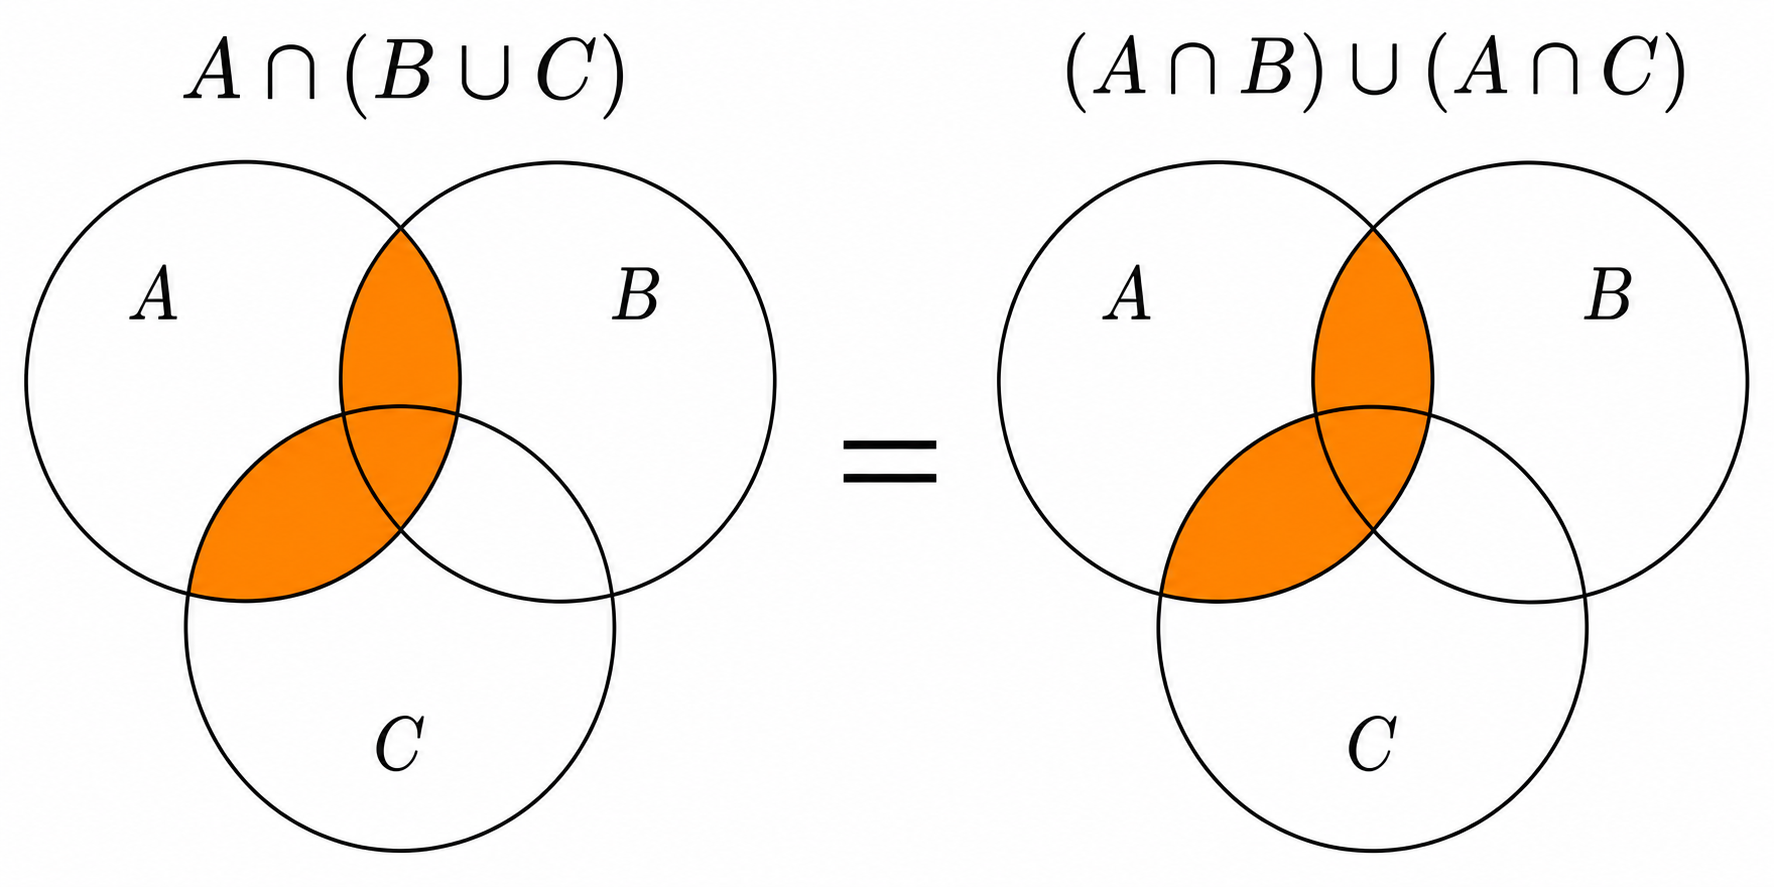
\includegraphics[width=0.65\textwidth]{Figures/png_ready/16-distributive-law-sets-generated.png}
    \caption{แผนภาพเวนน์แสดงกฎการแจกแจง $A \cap (B \cup C) = (A \cap B) \cup (A \cap C)$}
    \label{fig:distributive-law-sets}
\end{figure}

รูปที่ \ref{fig:distributive-law-sets} แสดงกฎการกระจายของเซต โดยฝั่งซ้ายแสดง $A \cap (B \cup C)$ และฝั่งขวาแสดง $(A \cap B) \cup (A \cap C)$ ทั้งสองให้ผลลัพธ์เดียวกัน

\section{กฎเดอมอร์แกน (De Morgan's Laws)}

กฎเดอมอร์แกนตั้งชื่อตามออกัสตัส เดอมอร์แกน (Augustus De Morgan, 1806--1871) นักคณิตศาสตร์ชาวอังกฤษ กฎนี้ระบุความสัมพันธ์ระหว่างคอมพลีเมนต์ ยูเนียน และอินเตอร์เซกชัน ใช้ในการพิสูจน์ทางคณิตศาสตร์และการแปลงนิพจน์ของวงจรดิจิทัล~\cite{halmos1974naive}

\begin{thrm}[กฎเดอมอร์แกนสำหรับเซต]
สำหรับทุกเซต $A$ และ $B$ จะได้ว่า
\begin{enumerate}
    \item $(A \cup B)^c = A^c \cap B^c$ นั่นคือคอมพลีเมนต์ของยูเนียนเท่ากับอินเตอร์เซกชันของคอมพลีเมนต์
    \item $(A \cap B)^c = A^c \cup B^c$ นั่นคือคอมพลีเมนต์ของอินเตอร์เซกชันเท่ากับยูเนียนของคอมพลีเมนต์
\end{enumerate}
\end{thrm}

อ่านกฎทั้งสองข้อเป็นภาษาพูดได้ว่า ข้อแรกคือ ``ไม่อยู่ใน $A$ หรือ $B$'' มีความหมายเดียวกับ ``ไม่อยู่ใน $A$ และไม่อยู่ใน $B$'' ส่วนข้อที่สองคือ ``ไม่อยู่ในทั้ง $A$ และ $B$ พร้อมกัน'' มีความหมายเดียวกับ ``ไม่อยู่ใน $A$ หรือไม่อยู่ใน $B$'' ข้อสังเกตสำคัญคือเมื่อกระจายคอมพลีเมนต์เข้าไปข้างใน ตัวดำเนินการจะสลับชนิดเสมอ ยูเนียนกลายเป็นอินเตอร์เซกชัน และอินเตอร์เซกชันกลายเป็นยูเนียน

\begin{rem}
สังเกตความสอดคล้องกับกฎเดอมอร์แกนในตรรกศาสตร์

\begin{enumerate}
    \item $\neg(p \land q) \equiv \neg p \lor \neg q$ สอดคล้องกับ $(A \cap B)^c = A^c \cup B^c$
    \item $\neg(p \lor q) \equiv \neg p \land \neg q$ สอดคล้องกับ $(A \cup B)^c = A^c \cap B^c$
\end{enumerate}
นี่เป็นตัวอย่างที่แสดงความเชื่อมโยงระหว่างตรรกศาสตร์และทฤษฎีเซต ทั้งสองระบบมีโครงสร้างทางคณิตศาสตร์ที่เหมือนกัน
\end{rem}

\begin{figure}[H]
    \centering
    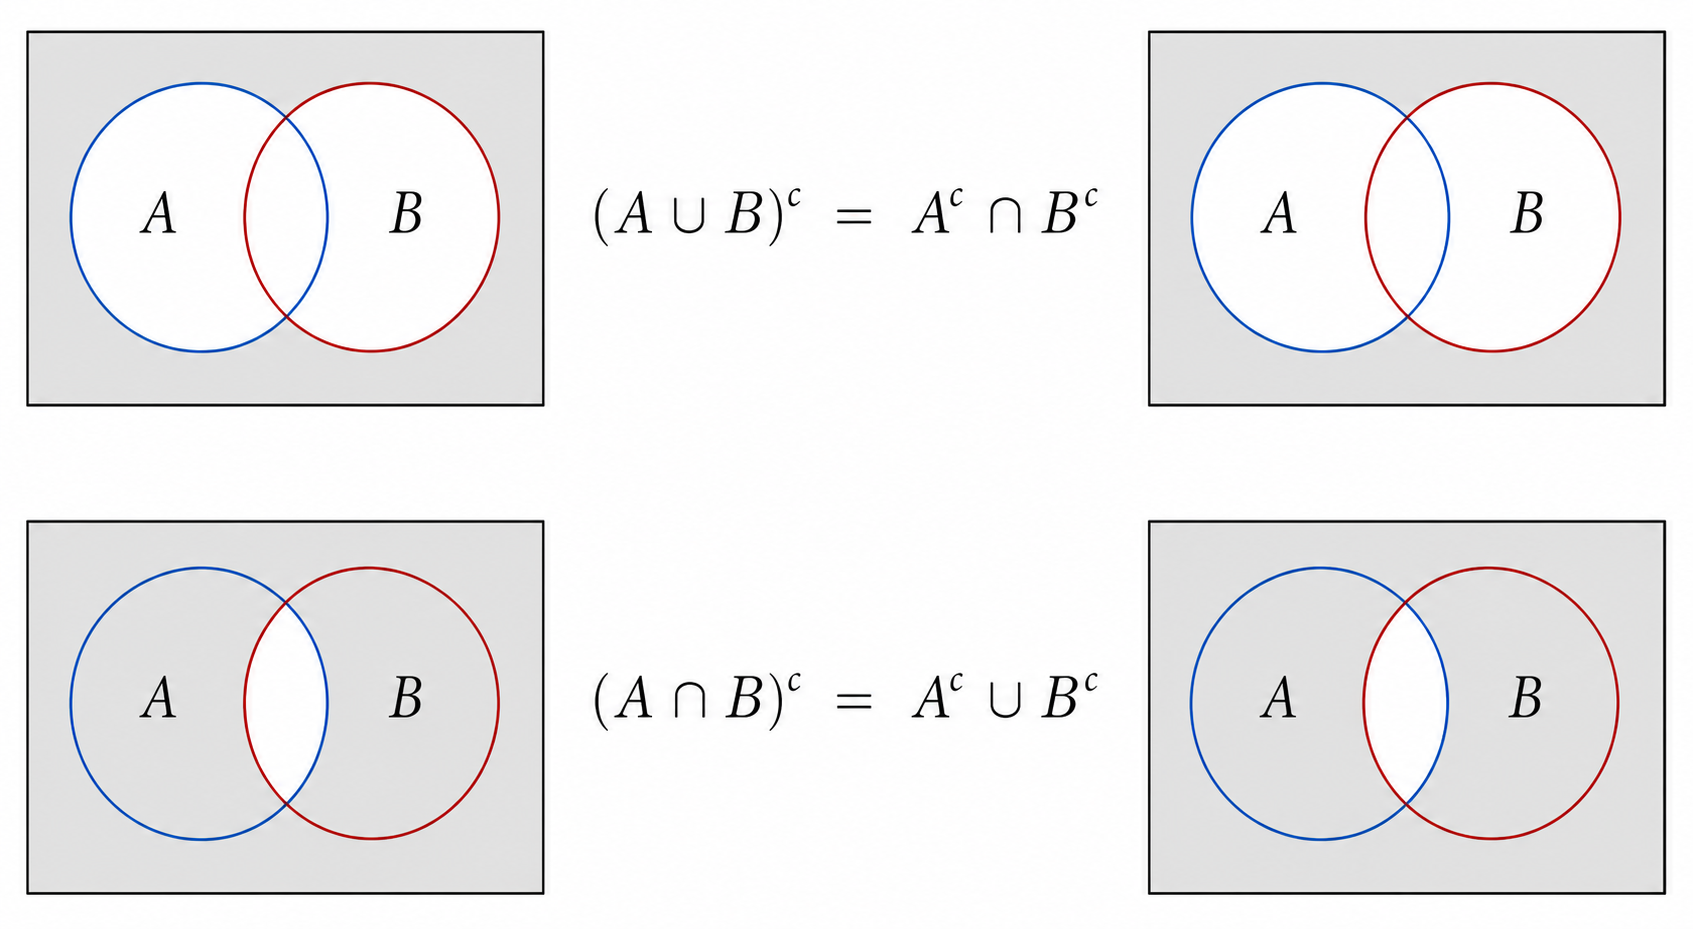
\includegraphics[width=0.65\textwidth]{Figures/png_ready/15-de-morgan-laws-generated.png}
    \caption{แผนภาพเวนน์แสดงกฎเดอมอร์แกน $(A \cup B)^c = A^c \cap B^c$ และ $(A \cap B)^c = A^c \cup B^c$}
    \label{fig:de-morgan-laws}
\end{figure}

รูปที่ \ref{fig:de-morgan-laws} แสดงกฎเดอมอร์แกนทั้งสองข้อ โดยฝั่งบนแสดงว่าคอมพลีเมนต์ของยูเนียนเท่ากับอินเตอร์เซกชันของคอมพลีเมนต์ และฝั่งล่างแสดงว่าคอมพลีเมนต์ของอินเตอร์เซกชันเท่ากับยูเนียนของคอมพลีเมนต์

กฎเดอมอร์แกนถูกนำไปใช้มากในการออกแบบวงจรดิจิทัล เพราะบางครั้งวงจรที่ออกแบบไว้ใช้ประตูตรรกะชนิดหนึ่ง แต่ชิ้นส่วนที่มีอยู่จริงเป็นอีกชนิดหนึ่ง กฎนี้ระบุวิธีแปลงประตูตรรกะแบบและให้เป็นประตูตรรกะแบบหรือโดยเพิ่มการนิเสธที่ขาเข้าและขาออก และแปลงย้อนกลับได้เช่นกัน โดยผลลัพธ์ของวงจรไม่เปลี่ยน รายละเอียดของการแปลงอยู่ใน\autoref{ch:boolean}

\begin{ex}[การพิสูจน์กฎเดอมอร์แกนข้อที่หนึ่ง]
พิสูจน์ $(A \cup B)^c = A^c \cap B^c$
\end{ex}
\begin{solution}
พิสูจน์แบบสมาชิก
\begin{align*}
x \in (A \cup B)^c
&\Leftrightarrow x \notin A \cup B\\
&\Leftrightarrow \neg(x \in A \lor x \in B)\\
&\Leftrightarrow \neg(x \in A) \land \neg(x \in B) \quad (\text{กฎเดอมอร์แกนของตรรกศาสตร์})\\
&\Leftrightarrow x \in A^c \land x \in B^c\\
&\Leftrightarrow x \in A^c \cap B^c
\end{align*}
$\therefore (A \cup B)^c = A^c \cap B^c$ \solhere
\end{solution}

\section{เพาเวอร์เซต (Power Set)}
บางครั้งเราไม่ได้สนใจเพียงสมาชิกของเซต แต่สนใจ ``เซตย่อยทั้งหมด'' ที่สร้างจากเซตนั้นได้ การรวบรวมเซตย่อยทุกแบบเข้าด้วยกันเป็นเซตใหม่ นำไปสู่แนวคิดเพาเวอร์เซต ประเด็นที่ต้องระวังคือสมาชิกของเพาเวอร์เซตเป็นเซต ไม่ใช่สมาชิกของเซตเดิม และเพาเวอร์เซตของเซตที่มีสมาชิก $n$ ตัวมีสมาชิกทั้งหมด $2^n$ ตัว ซึ่งเติบโตเร็วมากเมื่อ $n$ เพิ่มขึ้น~\cite{enderton1977settheory}

\begin{definition}[เพาเวอร์เซต]
\index{เพาเวอร์เซต!นิยาม}
เพาเวอร์เซต ของเซต $A$ เขียนแทนด้วย $\mathcal{P}(A)$ หรือ $2^A$ คือเซตที่ประกอบด้วยเซตย่อยทั้งหมดของ $A$ นั่นคือ
\[ \mathcal{P}(A) = \{B \mid B \subseteq A\} \]
\label{def:power-set}
\end{definition}

เพาเวอร์เซตเป็น ``เซตของเซต'' เพราะสมาชิกของมันคือเซตย่อยของ $A$ สมบัติสำคัญคือ ถ้า $|A| = n$ แล้ว $|\mathcal{P}(A)| = 2^n$ เหตุผลคือในการสร้างเซตย่อยหนึ่ง สมาชิกแต่ละตัวของ $A$ มีทางเลือก 2 ทาง คือ ``อยู่'' หรือ ``ไม่อยู่'' ในเซตย่อยนั้น จำนวนเซตย่อยทั้งหมดจึงเท่ากับ $2^n$ ด้วยเหตุนี้สัญลักษณ์ $2^A$ จึงสื่อความหมายได้ตรง เพราะ $|\mathcal{P}(A)| = 2^{|A|}$

\begin{ex}[การหาเพาเวอร์เซต]
จงหาเพาเวอร์เซตของเซตต่อไปนี้
\begin{enumerate}
    \item $\{1, 2\}$
    \item $\emptyset$
    \item $\{a\}$
    \item $\{1, 2, 3\}$
\end{enumerate}
\end{ex}
\begin{solution}
\begin{align*}
\mathcal{P}(\{1,2\}) &= \{\emptyset, \{1\}, \{2\}, \{1,2\}\} \quad (2^2 = 4)\\
\mathcal{P}(\emptyset) &= \{\emptyset\} \quad (2^0 = 1,\ \text{มีสมาชิกคือ } \emptyset)\\
\mathcal{P}(\{a\}) &= \{\emptyset, \{a\}\} \quad (2^1 = 2)\\
\mathcal{P}(\{1,2,3\}) &= \{\emptyset, \{1\}, \{2\}, \{3\}, \{1,2\}, \{1,3\}, \{2,3\}, \{1,2,3\}\} \quad (2^3 = 8)
\end{align*}
\solhere
\end{solution}


\section{ผลคูณคาร์ทีเซียน (Cartesian Product)}
\label{sec:cartesian-product}

การดำเนินการที่ผ่านมาทั้งหมดสร้างเซตใหม่จากสมาชิกชุดเดิม แต่ในการอธิบายความสัมพันธ์ระหว่างข้อมูลสองชุด สิ่งที่ต้องการคือการจับคู่สมาชิกจากเซตหนึ่งเข้ากับสมาชิกจากอีกเซตหนึ่ง เช่น การจับคู่รหัสนักศึกษากับรายวิชาที่ลงทะเบียน การจับคู่เช่นนี้ต้องรักษาลำดับไว้ เพราะคู่ที่ว่า ``นักศึกษา ก ลงทะเบียนวิชา ข'' ไม่เหมือนกับ ``วิชา ก ลงทะเบียนนักศึกษา ข'' หัวข้อนี้จึงเริ่มจากแนวคิดคู่อันดับ แล้วจึงนิยามผลคูณคาร์ทีเซียนซึ่งรวบรวมคู่อันดับที่เป็นไปได้ทั้งหมด แนวคิดนี้เป็นรากฐานโดยตรงของความสัมพันธ์และฟังก์ชันใน\autoref{ch:relations}

คู่อันดับ $(a, b)$ แตกต่างจากเซต $\{a, b\}$ ตรงที่มีลำดับ กล่าวคือ $(a, b) \neq (b, a)$ ยกเว้นกรณี $a = b$ และ $(a, b) = (c, d)$ ก็ต่อเมื่อ $a = c$ และ $b = d$ ชื่อผลคูณคาร์ทีเซียนมาจากชื่อของเรอเน เดการ์ต (Rene Descartes) นักคณิตศาสตร์ผู้พัฒนาเรขาคณิตวิเคราะห์ $\mathbb{R} \times \mathbb{R} = \mathbb{R}^2$ คือระนาบ 2 มิติที่เราใช้กันทั่วไป~\cite{lipschutz1998settheory}

\begin{definition}[ผลคูณคาร์ทีเซียน]
\index{ผลคูณคาร์ทีเซียน!นิยาม}
ผลคูณคาร์ทีเซียน ของเซต $A$ และ $B$ เขียนแทนด้วย $A \times B$ คือเซตของคู่อันดับ $(a, b)$ โดยที่ $a \in A$ และ $b \in B$ นั่นคือ
\[ A \times B = \{(a, b) \mid a \in A \text{ และ } b \in B\} \]
\end{definition}

\begin{ex}[การหาผลคูณคาร์ทีเซียน]
จงหาผลคูณคาร์ทีเซียนต่อไปนี้
\begin{enumerate}
    \item $\{1, 2\} \times \{a, b\}$
    \item $\mathbb{R} \times \mathbb{R}$
    \item $\emptyset \times A$ เมื่อ $A$ เป็นเซตใดๆ
\end{enumerate}
\end{ex}
\begin{solution}
\begin{align*}
\{1,2\} \times \{a,b\} &= \{(1,a),(1,b),(2,a),(2,b)\} \quad (\text{ลำดับสำคัญ เพราะ } (1,a) \neq (a,1))\\
\mathbb{R} \times \mathbb{R} &= \mathbb{R}^2 \quad (\text{ระนาบ 2 มิติ})\\
\emptyset \times A &= A \times \emptyset = \emptyset
\end{align*}
\solhere
\end{solution}

\begin{rem}[ข้อสังเกตเรื่องจำนวนสมาชิกของผลคูณคาร์ทีเซียน]
ถ้า $|A| = m$ และ $|B| = n$ แล้ว $|A \times B| = m \cdot n$ เพราะทุกสมาชิกใน $A$ สามารถจับคู่กับทุกสมาชิกใน $B$ ได้ จึงมี $m \times n$ คู่ และ $\mathbb{R} \times \mathbb{R}$ มี cardinality เท่ากับ $|\mathbb{R}|^2$ ซึ่งเป็น uncountable เช่นเดียวกับ $\mathbb{R}$
\end{rem}

\begin{prop}[สมบัติของผลคูณคาร์ทีเซียน]
ผลคูณคาร์ทีเซียนมีสมบัติดังนี้
\begin{enumerate}
    \item $A \times (B \cup C) = (A \times B) \cup (A \times C)$
    \item $A \times (B \cap C) = (A \times B) \cap (A \times C)$
    \item $(A \cup B) \times C = (A \times C) \cup (B \times C)$
    \item $(A \cap B) \times C = (A \times C) \cap (B \times C)$
\end{enumerate}
สังเกตว่า Cartesian Product กระจายเหนือ union และ intersection ในทางที่คล้ายกับการกระจายการคูณเหนือการบวก
\end{prop}

\section{การนับจำนวนสมาชิกของเซต (Cardinality)}

เมื่อมีเซตหนึ่ง คำถามพื้นฐานที่สุดคือเซตนั้นมีสมาชิกกี่ตัว การนับจำนวนสมาชิกเป็นสิ่งที่เราทำในชีวิตประจำวันอยู่แล้ว เช่น นับจำนวนนักศึกษาในห้องหรือจำนวนสินค้าในตะกร้า ในทางคณิตศาสตร์เรียกจำนวนสมาชิกของเซตว่าคาร์ดินัลลิตี้ สำหรับเซตจำกัดค่านี้เป็นจำนวนเต็มไม่ติดลบธรรมดา แต่สำหรับเซตอนันต์ต้องอาศัยการจับคู่หนึ่งต่อหนึ่งเพื่อเปรียบเทียบขนาด ซึ่งจะศึกษาในหัวข้อท้ายบท~\cite{rosen2019discrete}

\begin{definition}[จำนวนสมาชิกของเซต (Cardinality)]
\index{จำนวนสมาชิกของเซต!นิยาม}
จำนวนสมาชิกของเซต หรือคาร์ดินัลลิตี้ (cardinality) ของเซต $A$ เขียนแทนด้วย $|A|$ คือจำนวนสมาชิกของเซต $A$
\end{definition}

สำหรับเซตจำกัด จำนวนสมาชิกของเซตคือจำนวนที่นับได้โดยตรง เช่น ถ้า $A = \{a, e, i, o, u\}$ แล้ว $|A| = 5$ ส่วนเซตอนันต์ต้องใช้แนวคิดที่ละเอียดกว่านี้ คือการจับคู่สมาชิกแบบหนึ่งต่อหนึ่งระหว่างเซต และในบางกรณีต้องใช้ข้อโต้แย้งแนวทแยงของคันทอร์ (Cantor's diagonal argument) ซึ่งจะกล่าวถึงในหัวข้อเซตนับได้และเซตนับไม่ได้ต่อไป

การนับจำนวนสมาชิกเป็นพื้นฐานของการนับเชิงการจัด (combinatorics) และใช้มากในการนับจำนวนโอกาสทั้งหมดที่เป็นไปได้

\begin{principle}[หลักการรวม-การแยก (Inclusion-Exclusion Principle)]
สำหรับเซตจำกัด $A$ และ $B$ ใด ๆ จะได้ว่า
\begin{enumerate}
    \item $|A \cup B| = |A| + |B| - |A \cap B|$
    \item ถ้า $A$ และ $B$ เป็นเซตไม่มีสมาชิกร่วม คือ $A \cap B = \emptyset$ แล้ว $|A \cup B| = |A| + |B|$
\end{enumerate}
\end{principle}

\begin{figure}[H]
    \centering
    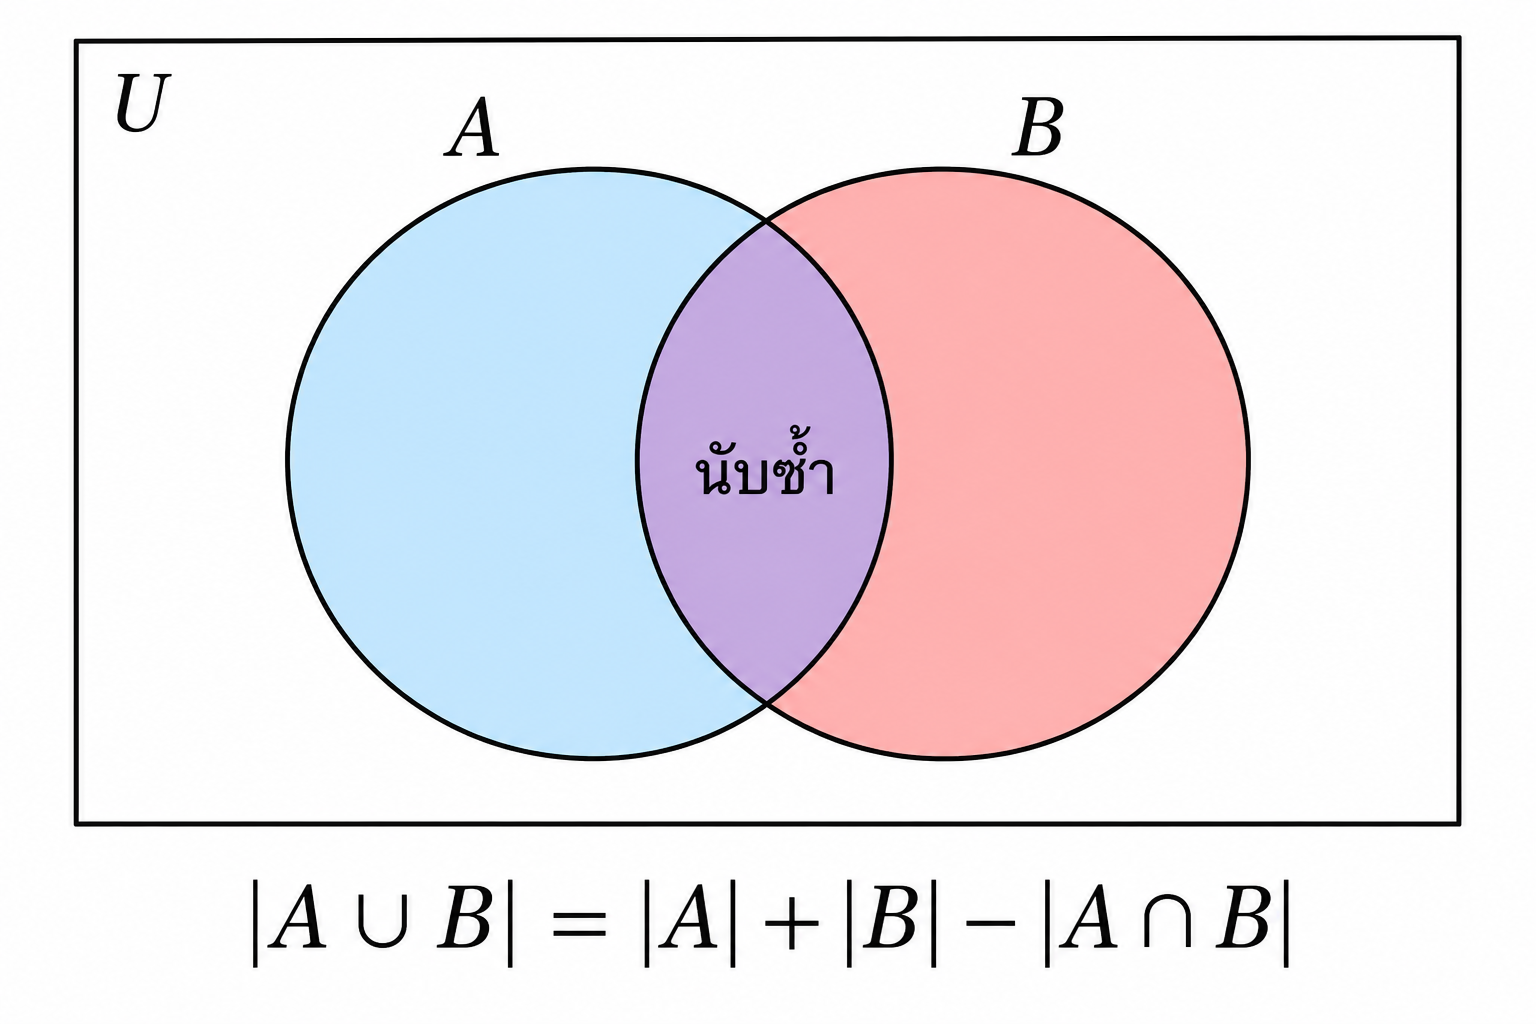
\includegraphics[width=0.70\textwidth]{Figures/png_ready/17-venn-inclusion-exclusion-generated.png}
    \caption{แผนภาพประกอบหลักการรวม-การแยก แสดงการหักส่วนซ้ำ $A\cap B$ ออกจาก $|A|+|B|$}
    \label{fig:venn-inclusion-exclusion}
\end{figure}

หลักการรวม-การแยกใช้เมื่อต้องการนับจำนวนสมาชิกของยูเนียน ถ้านับ $|A| + |B|$ โดยตรง สมาชิกที่อยู่ทั้งสองเซตจะถูกนับซ้ำ จึงต้องลบออก เหตุผลนี้เห็นได้ชัดจากรูปที่~\ref{fig:venn-inclusion-exclusion} ซึ่งพื้นที่ตรงกลางที่วงกลมสองวงซ้อนกันถูกระบายรวมอยู่ทั้งใน $|A|$ และ $|B|$ การบวกสองจำนวนนี้จึงนับพื้นที่ตรงกลางสองครั้ง การลบ $|A \cap B|$ ออกหนึ่งครั้งจึงทำให้ได้จำนวนที่ถูกต้องพอดี

\begin{ex}[การนับสมาชิกของยูเนียนด้วยหลักการเพิ่มเข้าตัดออก]
ถ้า $A = \{1, 2, 3, 4\}$, $B = \{3, 4, 5, 6\}$ จงหา $|A \cup B|$
\end{ex}
\begin{solution}
\begin{align*}
A \cap B &= \{3,4\} \Rightarrow |A \cap B| = 2\\
|A \cup B| &= |A| + |B| - |A \cap B| = 4 + 4 - 2 = 6
\end{align*}
ตรวจคำตอบได้จาก $|\{1,2,3,4,5,6\}| = 6$ ถ้านับ $|A|+|B| = 8$ โดยไม่หักส่วนที่ซ้อนกันออก ผลจะเกินจริง เพราะ 3 และ 4 ถูกนับสองครั้ง \solhere
\end{solution}

การประยุกต์ใช้ในชีวิตจริง ดังนี้

\begin{enumerate}
    \item นักศึกษา 30 คน 15 คนเรียนภาษาอังกฤษ 20 คนเรียนคณิตศาสตร์ มีนักศึกษากี่คนที่เรียนอย่างน้อยหนึ่งวิชา? ถ้าไม่มีนักศึกษาคนใดเรียนทั้งสองวิชา (disjoint) ก็ $15 + 20 = 35$ ซึ่งมากกว่า 30 แสดงว่าต้องมีนักศึกษาที่เรียนทั้งสองวิชา
\end{enumerate}

\begin{thrm}
สำหรับเซต 3 เซต ดังนี้

\[
|A \cup B \cup C| = |A| + |B| + |C| - |A \cap B| - |A \cap C| - |B \cap C| + |A \cap B \cap C|
\]

สูตรนี้ขยายจาก 2 เซต โดยลบ intersection ของทุกคู่ แล้วบวก intersection ของทั้งสามกลับ (เพราะถูกลบเกินไป)
\end{thrm}

\begin{ex}[ตัวอย่างตรวจพบข้อมูลไม่สอดคล้อง]
ในห้องเรียน 20 คน มี 12 คนเรียนคณิตศาสตร์ 15 คนเรียนฟิสิกส์ และ 10 คนเรียนเคมี นอกจากนี้ 6 คนเรียนคณิตศาสตร์และฟิสิกส์ 5 คนเรียนคณิตศาสตร์และเคมี 4 คนเรียนฟิสิกส์และเคมี และ 2 คนเรียนทั้งสามวิชา มีกี่คนที่เรียนอย่างน้อยหนึ่งวิชา?
\end{ex}
\begin{solution}
กำหนด $M$ (คณิตศาสตร์), $P$ (ฟิสิกส์), $C$ (เคมี) โดย $|M|=12$, $|P|=15$, $|C|=10$, $|M \cap P|=6$, $|M \cap C|=5$, $|P \cap C|=4$, $|M \cap P \cap C|=2$
\begin{align*}
|M \cup P \cup C| &= |M|+|P|+|C|-|M\cap P|-|M\cap C|-|P\cap C|+|M\cap P\cap C|\\
                  &= 12+15+10-6-5-4+2 = 24
\end{align*}
แต่ $24 > 20$ (จำนวนนักเรียนทั้งหมด) เป็นไปไม่ได้ แสดงว่าข้อมูลที่ให้มาไม่สอดคล้องกัน ควรย้อนกลับไปตรวจแหล่งข้อมูลก่อนสรุปผล \solhere
\end{solution}

\begin{thrm}[จำนวนสมาชิกของผลคูณคาร์ทีเซียน (Cardinality of Cartesian Product)]
\label{thrm:cardinality-cartesian}
ให้ $A$ และ $B$ เป็นเซตจำกัด (finite sets) ใด ๆ จำนวนสมาชิกของผลคูณคาร์ทีเซียน $A \times B$ จะเท่ากับผลคูณของจำนวนสมาชิกของเซต $A$ และเซต $B$ นั่นคือ
\[
|A \times B| = |A| \cdot |B|
\]
แนวคิดการพิสูจน์มีดังนี้ คู่อันดับ $(a, b) \in A \times B$ เกิดจากการเลือกสมาชิกตัวแรก $a$ จากเซต $A$ ซึ่งมีทางเลือก $|A|$ วิธี และเลือกสมาชิกตัวที่สอง $b$ จากเซต $B$ ซึ่งมีทางเลือก $|B|$ วิธี โดยการเลือกแต่ละตำแหน่งเป็นอิสระต่อกัน ตามหลักการคูณทางการนับ จะได้จำนวนคู่อันดับทั้งหมดเท่ากับ $|A| \cdot |B|$ ตัว
\end{thrm}

\begin{thrm}[จำนวนสมาชิกของเพาเวอร์เซต (Cardinality of Power Set)]
\label{thrm:cardinality-powerset}
ให้ $A$ เป็นเซตจำกัดที่มีสมาชิก $n$ ตัว นั่นคือ $|A| = n$ จำนวนสมาชิกของเพาเวอร์เซต $\mathcal{P}(A)$ (ซึ่งเท่ากับจำนวนสับเซตทั้งหมดของ $A$) จะเท่ากับ $2^n$ นั่นคือ
\[
|\mathcal{P}(A)| = 2^{|A|}
\]
แนวคิดการพิสูจน์มีดังนี้ ในการสร้างสับเซต $S \subseteq A$ สมาชิกแต่ละตัวใน $A$ มีทางเลือก 2 ทางเสมอ คือ ``เลือกให้อยู่ใน $S$'' หรือ ``ไม่เลือกให้อยู่ใน $S$'' เมื่อมีสมาชิกทั้งหมด $n$ ตัว การสร้างสับเซตจึงประกอบด้วยการตัดสินใจ $n$ ครั้งติดต่อกัน ตามหลักการคูณ จะได้จำนวนสับเซตที่เป็นไปได้ทั้งหมดเท่ากับ
\[
\underbrace{2 \times 2 \times \cdots \times 2}_{n \text{ ครั้ง}} = 2^n
\]
นอกจากนี้ ยังสามารถพิสูจน์ด้วยทฤษฎีบททวินาม (binomial theorem) จากการรวมจำนวนสับเซตที่มีขนาด $k$ (เลือกสมาชิก $k$ ตัวจาก $n$ ตัว) สำหรับ $k = 0, 1, \ldots, n$ จะได้
\[
|\mathcal{P}(A)| = \sum_{k=0}^{n} \binom{n}{k} = (1 + 1)^n = 2^n
\]
\end{thrm}

นี่เป็นเหตุผลว่าทำไมเพาเวอร์เซตจึงมีการเติบโตเชิงเลขชี้กำลัง (Exponential Growth) เมื่อ $|A|$ เพิ่มขึ้นเพียง 1 สมาชิก ขนาดของเพาเวอร์เซต $|\mathcal{P}(A)|$ จะเพิ่มขึ้นเป็น 2 เท่าเสมอ

\section{การประยุกต์ในวิทยาการคอมพิวเตอร์}

หัวข้อนี้แสดงการใช้แนวคิดเซตในวิทยาการคอมพิวเตอร์สามด้าน ได้แก่ การแทนเซตด้วยโครงสร้างข้อมูล การสืบค้นข้อมูลในฐานข้อมูล และการจัดเก็บสมาชิกด้วยฟังก์ชันแฮช~\cite{gersting2014structures}

\subsection{การแทนเซตในโครงสร้างข้อมูล}

ในการเขียนโปรแกรม การแทนเซตแต่ละวิธีใช้พื้นที่จัดเก็บและเวลาตรวจสอบสมาชิกต่างกัน การเลือกวิธีขึ้นกับขนาดของเอกภพสัมพัทธ์และการดำเนินการที่ต้องใช้ หัวข้อนี้อธิบายการแทนเซตด้วยเวกเตอร์บิตและตารางแฮช~\cite{gersting2014structures}

\begin{ex}[การแทนด้วยเวกเตอร์บิต (Bit Vector Representation)]
จงแทนเซต $A = \{2, 5, 7\}$ ในเอกภพสัมพัทธ์ $U = \{1, 2, 3, 4, 5, 6, 7, 8, 9\}$ ด้วยเวกเตอร์บิต
\end{ex}
\begin{solution}
กำหนดบิตตามตำแหน่งของสมาชิกใน $U = \{1,2,\ldots,9\}$ โดยให้บิตมีค่า 1 เมื่อสมาชิกอยู่ใน $A = \{2,5,7\}$ และมีค่า 0 เมื่อสมาชิกไม่อยู่ใน $A$
\begin{center}
$U$:\quad \texttt{1 2 3 4 5 6 7 8 9}\\[2pt]
$A$:\quad \texttt{0 1 0 0 1 0 1 0 0}
\end{center}
ได้เวกเตอร์บิต $\texttt{010010100}$ ซึ่งมีค่าเท่ากับ $148_{10}$ เมื่อมองเป็นจำนวนฐานสอง การตรวจสอบสมาชิกทำได้โดยอ่านบิตที่ตำแหน่งนั้น จึงใช้เวลา $O(1)$ การยูเนียน อินเตอร์เซกชัน และคอมพลีเมนต์ดำเนินการแบบบิตต่อบิต จึงใช้เวลา $O(n)$ สำหรับเวกเตอร์ที่มีความยาว $n$ \solhere
\end{solution}

\begin{principle}[การดำเนินการของเซตในรูปพีชคณิตบูลีน (Set Operations as Boolean Algebra)]
เซตบนเอกภพสัมพัทธ์ที่มีขนาด $n$ แทนได้ด้วยเวกเตอร์บิตความยาว $n$ การดำเนินการระหว่างเซตจึงสอดคล้องกับพีชคณิตบูลีน ดังนี้

\begin{enumerate}
    \item $A \cup B$ $\Leftrightarrow$ OR แบบบิตต่อบิตของเวกเตอร์บิต
    \item $A \cap B$ $\Leftrightarrow$ AND แบบบิตต่อบิตของเวกเตอร์บิต
    \item $A^c$ $\Leftrightarrow$ NOT แบบบิตต่อบิตของเวกเตอร์บิต
    \item $A \subseteq B$ $\Leftrightarrow$ $(A \cap B^c) = \emptyset$ หรือไม่มีตำแหน่งใดที่บิตของ $A$ เป็น 1 แต่บิตของ $B$ เป็น 0
\end{enumerate}

ความสอดคล้องนี้เชื่อมทฤษฎีเซตกับพีชคณิตบูลีนและตรรกศาสตร์เชิงประพจน์
\label{theo:set-boolean-algebra}
\end{principle}

\subsection{การประยุกต์ในฐานข้อมูล}

ในแบบจำลองฐานข้อมูลเชิงสัมพันธ์ ความสัมพันธ์ (relation) เป็นเซตของคู่อันดับหรือทูเพิล (tuple) พีชคณิตเชิงสัมพันธ์ (relational algebra) จึงใช้การดำเนินการที่เชื่อมโยงกับทฤษฎีเซต ดังแสดงในตารางที่ \ref{tab:relalg-sets} ระบบฐานข้อมูลเชิงปฏิบัติอาจอนุญาตให้มีแถวซ้ำได้ จึงต้องพิจารณากติกาของระบบเมื่อใช้คำสั่งสืบค้น~\cite{codd1970relational}

\begin{table}[H]
\centering
\caption{ความสัมพันธ์ระหว่าง Relational Algebra และ Set Theory}
\label{tab:relalg-sets}
\renewcommand{\arraystretch}{1.3}
\begin{tabular}{|c|c|}
\hline
\cellcolor{navy}\textcolor{white}{\textbf{พีชคณิตเชิงสัมพันธ์}} & \cellcolor{navy}\textcolor{white}{\textbf{ทฤษฎีเซต}} \\
\hline
Union ($\cup$) & การยูเนียน (Union) \\
Selection ($\sigma$) & การกรองด้วยเงื่อนไข / สับเซต (Filtering / Subset) \\
Projection ($\pi$) & การเลือกเฉพาะคอมโพเนนต์ (Domain Restriction) \\
Cartesian Product ($\times$) & ผลคูณคาร์ทีเซียน (Cartesian Product) \\
Join ($\bowtie$) & การรวมเซตแบบมีเงื่อนไข (Complex Combination) \\
\hline
\end{tabular}
\end{table}

\begin{ex}[ความสัมพันธ์ในฐานข้อมูลในรูปเซตคณิตศาสตร์]
จงอธิบายว่าเซตและความสัมพันธ์ทางคณิตศาสตร์เกี่ยวข้องอย่างไรกับฐานข้อมูลเชิงสัมพันธ์
\end{ex}
\begin{solution}
ในเชิงเซต ความสัมพันธ์ $R$ เป็นเซตของทูเพิล โดย $R \subseteq D_1 \times D_2 \times \cdots \times D_n$ และ $D_i$ เป็นโดเมนของแอตทริบิวต์ลำดับที่ $i$ คีย์หลัก (primary key) เป็นกลุ่มแอตทริบิวต์ที่ระบุทูเพิลได้เฉพาะเจาะจง ส่วนคีย์นอก (foreign key) อ้างอิงคีย์หลักของความสัมพันธ์อื่น ตัวอย่างเช่น ถ้า $S$ เป็นเซตของนักศึกษา $C$ เป็นเซตของรายวิชา และ $E \subseteq S \times C$ เป็นเซตของการลงทะเบียนแล้ว $E$ คือเซตของทูเพิล $(s,c)$ ที่ $s \in S$ และ $c \in C$ ดังนั้น $E$ เป็นเซตย่อยของผลคูณคาร์ทีเซียน $S \times C$ \solhere
\end{solution}

\subsection{ตารางแฮชและฟังก์ชันแฮช (Hash Table)}
ตารางแฮช (Hash Table) เป็นโครงสร้างข้อมูลที่ใช้ฟังก์ชันแฮชส่งคีย์จากเอกภพของคีย์ไปยังตำแหน่งดรรชนีในหน่วยความจำ จึงใช้เก็บ ตรวจสอบ เพิ่ม และลบสมาชิกของเซตได้ การดำเนินการเหล่านี้มีความซับซ้อนเชิงเวลาเฉลี่ยระดับคงที่เมื่อฟังก์ชันแฮชกระจายคีย์ได้เหมาะสม ดังแสดงในตารางที่~\ref{tab:hash-complexity}~\cite{gersting2014structures}

\begin{definition}[ฟังก์ชันแฮชในฐานะฟังก์ชันทางคณิตศาสตร์ (Hash Function)]
ฟังก์ชันแฮช $h: U \rightarrow \{0, 1, \ldots, m-1\}$ เป็นฟังก์ชันจากเอกภพของคีย์ $U$ ไปยังเซตของตำแหน่งจัดเก็บ $\{0, 1, \ldots, m-1\}$

ฟังก์ชันแฮชที่ดีควรมีสมบัติดังนี้
\begin{enumerate}
    \item ให้ผลแน่นอน (deterministic) ถ้า $k_1 = k_2$ แล้ว $h(k_1) = h(k_2)$
    \item กระจายคีย์สม่ำเสมอ (uniformly distributed) ค่าของ $h(k)$ ควรกระจายทั่ว $\{0, 1, \ldots, m-1\}$
    \item คำนวณได้รวดเร็ว (efficiently computable) คำนวณค่าแฮชของคีย์หนึ่งตัวได้ในเวลา $O(1)$
\end{enumerate}

เมื่อเกิดการชนกัน (collision) ที่ $h(k_1) = h(k_2)$ สำหรับ $k_1 \neq k_2$ สามารถจัดการได้ดังนี้
\begin{enumerate}
    \item การเชื่อมโยงรายการ (chaining) $T[i] = \{k \in K \mid h(k) = i\}$ โดยแต่ละตำแหน่งเก็บคีย์ที่มีค่าแฮชเดียวกัน
    \item การกำหนดตำแหน่งเปิด (open addressing) ใช้ลำดับการตรวจตำแหน่ง $h(k, i) = (h'(k) + i) \mod m$ สำหรับ $i = 0, 1, 2, \ldots$
\end{enumerate}
\label{theo:hash-function}
\end{definition}

ประสิทธิภาพของการดำเนินการทางเซตเมื่อใช้โครงสร้างข้อมูลประเภทตารางแฮช (Hash Set) เป็นไปตามสมบัติความซับซ้อนเชิงเวลา ดังแสดงในตารางที่ \ref{tab:hash-complexity}

\begin{table}[H]
\centering
\caption{ความซับซ้อนเชิงเวลา (Time Complexity) ของ Hash Set Operations}
\label{tab:hash-complexity}
\renewcommand{\arraystretch}{1.3}
\begin{tabular}{|l|c|}
\hline
\cellcolor{navy}\textcolor{white}{\textbf{การดำเนินการ (Operation)}} & \cellcolor{navy}\textcolor{white}{\textbf{ความซับซ้อนเชิงเวลา (Time Complexity)}} \\
\hline
การตรวจสอบสมาชิก ($x \in A$) & $O(1)$ \\
การเพิ่มสมาชิก ($A \cup \{x\}$) & $O(1)$ \\
การลบสมาชิก ($A - \{x\}$) & $O(1)$ \\
การยูเนียน ($A \cup B$) & $O(|A| + |B|)$ \\
การอินเตอร์เซกชัน ($A \cap B$) & $O(\min(|A|, |B|))$ \\
การทดสอบเซตย่อย ($A \subseteq B$) & $O(|A|)$ \\
\hline
\end{tabular}
\end{table}

% ===================== SECTION 10: เซตที่นับได้และเซตที่นับไม่ได้ =====================
\section{เซตที่นับได้และเซตที่นับไม่ได้}
\label{sec:countable-uncountable}

เซตอนันต์แบ่งเป็นเซตนับได้ (Countable) และเซตนับไม่ได้ (Uncountable) เซตนับได้มีฟังก์ชันหนึ่งต่อหนึ่งจากเซตไปยังเซตย่อยของ $\mathbb{N}$ ตัวอย่างเช่น เซตจำนวนเต็มและเซตจำนวนตรรกยะเป็นเซตนับได้ ส่วนเซตจำนวนจริงเป็นเซตนับไม่ได้ ความแตกต่างนี้เชื่อมโยงกับวิทยาการคอมพิวเตอร์ เพราะเซตของโปรแกรมที่เขียนได้เป็นเซตนับได้ แต่เซตของฟังก์ชันจากจำนวนนับไปยังจำนวนนับเป็นเซตนับไม่ได้ จึงมีฟังก์ชันที่ไม่มีโปรแกรมใดคำนวณได้~\cite{epp2019discrete}

\index{เซตนับได้}\index{countable set}
\index{เซตนับไม่ได้}\index{uncountable set}
\index{$\aleph_0$}
\index{$\mathfrak{c}$}
\begin{definition}[เซตนับได้และเซตนับไม่ได้]
เซต $A$ เป็น \textbf{เซตนับได้} (countable) ก็ต่อเมื่อ $|A| \leq |\mathbb{N}|$ หรือกล่าวอีกนัยหนึ่งคือมีฟังก์ชันหนึ่งต่อหนึ่งจาก $A$ ไปยังเซตย่อยของ $\mathbb{N}$ ถ้า $A$ ไม่นับได้ เราเรียกว่า $A$ เป็น \textbf{เซตนับไม่ได้} (uncountable)
\end{definition}

คันทอร์พิสูจน์ว่าช่วงเปิด $(0, 1)$ ของจำนวนจริงเป็นเซตนับไม่ได้ด้วยวิธีเส้นทแยงมุม (Diagonal Argument)~\cite{enderton1977settheory}

\begin{thrm}[ทฤษฎีบทของคันทอร์]
\index{ทฤษฎีบทของคันทอร์}
ช่วงเปิด $(0, 1)$ ของจำนวนจริงเป็นเซตนับไม่ได้
\end{thrm}

\begin{ex}[การจำแนกเซตนับได้และเซตนับไม่ได้]
จงจำแนกว่าเซตใดนับได้และเซตใดนับไม่ได้
\end{ex}
\begin{solution}
\begin{align*}
\text{(ก)}\ \ \mathbb{N} &\ \text{นับได้} \quad (|\mathbb{N}| = \aleph_0)\\
\text{(ข)}\ \ \mathbb{Z} &\ \text{นับได้} \quad (\text{จับคู่ } 0{\leftrightarrow}1,\ 1{\leftrightarrow}2,\ -1{\leftrightarrow}3,\ 2{\leftrightarrow}4,\ldots)\\
\text{(ค)}\ \ \mathbb{Q} &\ \text{นับได้} \quad (\text{หนาแน่นในจำนวนจริง แต่ยังนับได้})\\
\text{(ง)}\ \ \mathbb{R} &\ \text{นับไม่ได้} \quad (|\mathbb{R}| = \mathfrak{c} > \aleph_0)
\end{align*}
\solhere
\end{solution}

\sectionbanner{สรุปบทเรียน}
บทนี้เริ่มจากนิยามของเซตและสมาชิก ซึ่งข้อกำหนดสำคัญคือเงื่อนไขการเป็นสมาชิกต้องชัดเจนพอที่จะตัดสินได้โดยไม่ขึ้นกับความเห็นของผู้ตัดสิน การเขียนเซตทำได้สองวิธี คือวิธีแจกแจงสมาชิกซึ่งเหมาะกับเซตขนาดเล็ก และวิธีกำหนดสมบัติซึ่งใช้ได้แม้เซตมีสมาชิกไม่สิ้นสุด นอกจากนี้ยังมีเซตพิเศษที่ใช้อ้างอิงตลอดทั้งเล่ม ได้แก่ เซตว่างและเอกภพสัมพัทธ์

ความสัมพันธ์ระหว่างเซตอธิบายด้วยเซตย่อยและเซตย่อยแท้ โดยการพิสูจน์ว่าสองเซตเท่ากันใช้วิธีบรรจุสองทาง คือแสดงว่าแต่ละเซตเป็นเซตย่อยของอีกเซตหนึ่ง ส่วนการดำเนินการระหว่างเซตมีสี่ชนิดหลัก ได้แก่ ยูเนียน อินเตอร์เซกชัน ผลต่าง และคอมพลีเมนต์ ซึ่งสอดคล้องกับตัวเชื่อมทางตรรกศาสตร์ใน\autoref{ch:logic} คือการเชื่อมแบบหรือ การเชื่อมแบบและ และนิเสธ ตามลำดับ กฎพีชคณิตของเซตจึงเป็นกฎชุดเดียวกับกฎพีชคณิตของประพจน์ รวมทั้งกฎเดอมอร์แกนที่โยงคอมพลีเมนต์เข้ากับยูเนียนและอินเตอร์เซกชัน

ส่วนที่เหลือของบทว่าด้วยการสร้างเซตใหม่และการนับ เพาเวอร์เซตรวบรวมเซตย่อยทั้งหมดและมีสมาชิก $2^{|A|}$ ตัว ผลคูณคาร์ทีเซียนสร้างเซตของคู่อันดับและมีสมาชิก $|A| \cdot |B|$ ตัว ซึ่งเป็นรากฐานของความสัมพันธ์และฟังก์ชันใน\autoref{ch:relations} ส่วนหลักการรวม-การแยก $|A \cup B| = |A| + |B| - |A \cap B|$ ใช้นับสมาชิกของยูเนียนโดยไม่นับส่วนที่ซ้อนกันซ้ำ ปิดท้ายด้วยการจำแนกเซตนับได้กับเซตนับไม่ได้ และการประยุกต์ในวิทยาการคอมพิวเตอร์ทั้งด้านโครงสร้างข้อมูล ฐานข้อมูลเชิงสัมพันธ์ และตารางแฮช

ทฤษฎีเซตเป็นพื้นฐานของบทถัดไป โดยเฉพาะความสัมพันธ์ซึ่งอาศัยผลคูณคาร์ทีเซียน และฟังก์ชันซึ่งเป็นกรณีเฉพาะของความสัมพันธ์ ภาษาของเซตยังเป็นภาษาที่ใช้ร่วมกันในทุกสาขาของคณิตศาสตร์~\cite{rosen2019discrete}

\clearpage
\sectionbanner{แบบฝึกหัด}

\exercisepart{ส่วนที่ 1 นิยามพื้นฐาน}
\begin{exercise}
เขียนเซตต่อไปนี้โดยใช้ทั้งวิธีแจกแจงสมาชิกและวิธีกำหนดสมบัติ
\begin{enumerate}
    \item เซตของจำนวนเต็มบวกที่น้อยกว่า 10
    \item เซตของจำนวนเฉพาะที่น้อยกว่า 20
    \item เซตของสระในภาษาอังกฤษ
    \item เซตของจำนวนเต็ม $x$ ที่ $x^2 - 4 = 0$
    \item เซตของจำนวนเต็ม $x$ ที่ $x^2 - 5x + 6 = 0$
\end{enumerate}
\end{exercise}

\begin{exercise}
กำหนดให้ $A = \{1, 2, 3\}$, $B = \{3, 4, 5\}$, $C = \{5, 6\}$ จงหาผลของการดำเนินการต่อไปนี้
\begin{enumerate}
    \item $A \cup B$
    \item $A \cap B$
    \item $A - B$
    \item $B - A$
    \item $(A \cup B) - C$
    \item $A \cap (B \cup C)$
    \item $(A - B) \cup (B - A)$
    \item $A \cap B \cap C$
    \item $(A \cup B) \cap (B \cup C)$
\end{enumerate}
\end{exercise}

\begin{exercise}
จงพิจารณาว่าข้อความต่อไปนี้จริงหรือเท็จ พร้อมอธิบายเหตุผล
\begin{enumerate}
    \item $\emptyset \in \{\emptyset\}$
    \item $\emptyset \subseteq \{\emptyset\}$
    \item $\{\emptyset\} \in \{\emptyset, \{\emptyset\}\}$
    \item $\{1, 2\} \subseteq \{\{1\}, \{2\}\}$
    \item $\{1, 2\} \in \{\{1, 2\}\}$
    \item $|\mathcal{P}(\{1, 2, 3\})| = 8$
    \item $\mathcal{P}(\emptyset) = \emptyset$
    \item $\{1, 2\} \times \{3, 4\} = \{3, 4\} \times \{1, 2\}$
\end{enumerate}
\end{exercise}

\begin{exercise}
อธิบายความแตกต่างระหว่าง $\in$ และ $\subseteq$ พร้อมยกตัวอย่างที่แสดงความแตกต่างนั้น
\end{exercise}

\exercisepart{ส่วนที่ 2 การพิสูจน์}
\begin{exercise}
จงพิสูจน์ข้อความต่อไปนี้ด้วยการพิสูจน์ตรง
\begin{enumerate}
    \item ถ้า $A \subseteq B$ และ $B \subseteq C$ แล้ว $A \subseteq C$ (Transitivity ของ $\subseteq$)
    \item ถ้า $A \subseteq B$ แล้ว $A \cup C \subseteq B \cup C$
    \item ถ้า $A \subseteq B$ แล้ว $A \cap C \subseteq B \cap C$
    \item $A \cup (B \cap C) = (A \cup B) \cap (A \cup C)$ (Distributive Law ข้อ 2)
\end{enumerate}
\end{exercise}

\begin{exercise}
จงพิสูจน์ข้อความต่อไปนี้ด้วยการพิสูจน์แบบแย้งสลับที่
\begin{enumerate}
    \item ถ้า $A \cup B \neq A$ แล้ว $B \not\subseteq A$
    \item ถ้า $A \cap B = \emptyset$ แล้ว $A \subseteq B^c$
    \item ถ้า $A \not\subseteq B \cup C$ แล้ว $A \not\subseteq B$ และ $A \not\subseteq C$
\end{enumerate}
\end{exercise}

\begin{exercise}
จงพิสูจน์ข้อความต่อไปนี้ด้วยการพิสูจน์โดยข้อขัดแย้ง
\begin{enumerate}
    \item ถ้า $A \subseteq B$ แล้ว $B^c \subseteq A^c$
    \item ถ้า $A \cup B = A \cap B$ แล้ว $A = B$
    \item สำหรับเซตจำกัด $A$ จะได้ $|A| < |\mathcal{P}(A)|$
\end{enumerate}
\end{exercise}

\begin{exercise}
จงพิสูจน์ว่าเซตต่อไปนี้เท่ากัน
\begin{enumerate}
    \item $A - (B \cup C) = (A - B) \cap (A - C)$
    \item $A \Delta B = (A \cup B) - (A \cap B)$ (Symmetric Difference)
    \item $(A - B) \cap C = (A \cap C) - B$
\end{enumerate}
\end{exercise}

\exercisepart{ส่วนที่ 3 กฎเดอมอร์แกนและการดำเนินการ}
\begin{exercise}
จงพิสูจน์กฎเดอมอร์แกนต่อไปนี้
\begin{enumerate}
    \item $(A \cap B)^c = A^c \cup B^c$
    \item $(A \cup B)^c = A^c \cap B^c$
\end{enumerate}
\end{exercise}

\begin{exercise}
จงลดรูปเซตต่อไปนี้ให้อยู่ในรูปที่ง่ายที่สุด
\begin{enumerate}
    \item $(A \cup B) \cap (A \cup B^c)$
    \item $(A - B) \cup (A \cap B)$
    \item $A \cup (B - A)$
    \item $(A \cap B) \cup (A - B)$
    \item $A \cap (A \cup B)$
    \item $(A^c)^c$
\end{enumerate}
\end{exercise}

\begin{exercise}
กำหนดให้ $A$, $B$, $C$ เป็นเซตย่อยของเอกภพสัมพัทธ์ $U$ พิจารณาว่าข้อความต่อไปนี้จริงหรือเท็จ พร้อมพิสูจน์หรือยกตัวอย่างค้าน
\begin{enumerate}
    \item $A - B = B - A$
    \item $A \cup B = A \cap B$ แก้สมการนี้
    \item $(A - B) - C = A - (B - C)$
\end{enumerate}
\end{exercise}

\exercisepart{ส่วนที่ 4 เพาเวอร์เซตและคาร์ทีเซียน}
\begin{exercise}
จงหาผลลัพธ์ต่อไปนี้
\begin{enumerate}
    \item $\mathcal{P}(\{a, b, c\})$
    \item $|\mathcal{P}(\mathcal{P}(\emptyset))|$
    \item $\{1, 2\} \times \{3, 4, 5\}$
    \item $|\{1, 2\} \times \{3, 4\} \times \{5, 6\}|$
    \item $\mathcal{P}(\{1, 2\}) \cap \mathcal{P}(\{2, 3\})$
    \item $\mathcal{P}(\{1, 2\}) \cup \mathcal{P}(\{2, 3\})$
\end{enumerate}
\end{exercise}

\begin{exercise}
จงพิสูจน์ข้อความต่อไปนี้
\begin{enumerate}
    \item $\mathcal{P}(A) \cup \mathcal{P}(B) \subseteq \mathcal{P}(A \cup B)$
    \item จงพิสูจน์หรือยกตัวอย่างค้านของ $\mathcal{P}(A \cup B) \subseteq \mathcal{P}(A) \cup \mathcal{P}(B)$
    \item $(A \times B) \cap (C \times D) = (A \cap C) \times (B \cap D)$
\end{enumerate}
\end{exercise}

\begin{exercise}
ถ้า $|A| = 3$ และ $|B| = 4$ จงหาผลลัพธ์ต่อไปนี้
\begin{enumerate}
    \item $|A \times B|$
    \item $|\mathcal{P}(A)|$
    \item $|\mathcal{P}(A \times B)|$
    \item $|\mathcal{P}(A) \times \mathcal{P}(B)|$
\end{enumerate}
\end{exercise}

\begin{exercise}
อธิบายว่าทำไม $|\mathcal{P}(A)| > |A|$ สำหรับทุกเซต $A$ ที่ไม่ใช่เซตว่าง (ทฤษฎีบทของคันทอร์)
\end{exercise}

\exercisepart{ส่วนที่ 5 การประยุกต์และการเชื่อมโยงทางคณิตศาสตร์}
\begin{exercise}
กำหนดให้ $A = \{10, 20, 30, 40\}$ และ $B = \{25, 30, 35, 40\}$ ในฐานข้อมูล จงเขียนในรูปแบบคณิตศาสตร์
\begin{enumerate}
    \item จงหา $A \cup B$, $A \cap B$, $A - B$, $A \Delta B$ (Symmetric Difference)
    \item แสดงว่า $A \Delta B = (A \cup B) - (A \cap B)$
\end{enumerate}
\end{exercise}

\begin{exercise}
กำหนดให้ $U = \{1, 2, 3, 4, 5, 6, 7, 8, 9, 10\}$ และ $A = \{1, 2, 3, 4, 5\}$, $B = \{4, 5, 6, 7\}$
\begin{enumerate}
    \item เขียน bit vector ของ $A$, $B$, $A \cup B$, $A \cap B$, $A^c$
    \item แสดงว่า bitwise operations บน bit vectors ให้ผลลัพธ์ที่ถูกต้องสำหรับ set operations
\end{enumerate}
\end{exercise}

\begin{exercise}
จงอธิบายความสัมพันธ์ระหว่างสิ่งต่อไปนี้
\begin{enumerate}
    \item กฎเดอมอร์แกนในทฤษฎีเซต และกฎเดอมอร์แกนในตรรกศาสตร์
    \item Cartesian Product $A \times B$ และ relations ระหว่างเซต
    \item เพาเวอร์เซต $\mathcal{P}(A)$ กับจำนวนสมาชิกของเพาเวอร์เซต $|\mathcal{P}(A)| = 2^{|A|}$
\end{enumerate}
\end{exercise}

\begin{exercise}
จงพิสูจน์ข้อความต่อไปนี้โดยใช้ทฤษฎีเซต
\begin{enumerate}
    \item ถ้า $A \subseteq B$ แล้ว $\mathcal{P}(A) \subseteq \mathcal{P}(B)$
    \item ถ้า $A \times B = A \times C$ และ $A \neq \emptyset$ แล้ว $B = C$
\end{enumerate}
\end{exercise}

\answerkeyhead
\exercisepart{เฉลยส่วนที่ 1 แนวคิดพื้นฐานและการระบุเซต}
\begin{enumerate}[label={},leftmargin=0pt,itemsep=0.6em]
    \item
    \begin{enumerate}[label=\textbf{\thechapter.\arabic{enumi}.\arabic*}]
        \item $\{1, 2, 3, 4, 5, 6, 7, 8, 9\} = \{x \in \mathbb{N} \mid x < 10\}$
        \item $\{2, 3, 5, 7, 11, 13, 17, 19\} = \{p \in \mathbb{N} \mid p \text{ เป็นจำนวนเฉพาะ และ } p < 20\}$
        \item $\{a, e, i, o, u\}$
        \item $\{-2, 2\} = \{x \in \mathbb{Z} \mid x^2 = 4\}$
        \item $\{2, 3\} = \{x \in \mathbb{Z} \mid x^2 - 5x + 6 = 0\}$
    \end{enumerate}

    \item
    \begin{enumerate}[label=\textbf{\thechapter.\arabic{enumi}.\arabic*}]
        \item $\{1, 2, 3, 4, 5\}$
        \item $\{3\}$
        \item $\{1, 2\}$
        \item $\{4, 5\}$
        \item $\{1, 2, 3, 4\}$
        \item $\{3, 5\}$
        \item $\{1, 2, 4, 5\}$
        \item $\{5\}$
        \item $\{3, 4, 5\}$
    \end{enumerate}

    \item
    \begin{enumerate}[label=\textbf{\thechapter.\arabic{enumi}.\arabic*}]
        \item จริง ($\emptyset \in \{\emptyset\}$ เพราะเซตว่างปรากฏเป็นสมาชิกในนั้น)
        \item จริง ($\emptyset \subseteq A$ สำหรับทุกเซต $A$)
        \item จริง ($\{\emptyset\} \in \{\emptyset, \{\emptyset\}\}$)
        \item เท็จ ($\{1\} \not\subseteq \{1, 2\}$ แต่ $1 \in \{1, 2\}$)
        \item เท็จ ($\{1, 2\} \neq \{\{1, 2\}\}$)
        \item จริง ($|\{1, 2, 3\}| = 3$ ดังนั้น $|\mathcal{P}(A)| = 2^3 = 8$)
        \item เท็จ ($\mathcal{P}(\emptyset) = \{\emptyset\} \neq \emptyset$)
        \item เท็จ ($(1, 3) \neq (3, 1)$ Cartesian Product ไม่มีสมบัติสลับที่)
    \end{enumerate}
\end{enumerate}

\exercisepart{เฉลยส่วนที่ 2 การดำเนินการบนเซตและสับเซต}
\begin{enumerate}[label={},leftmargin=0pt,itemsep=0.6em]
    \setcounter{enumi}{3}
    \item
    \begin{enumerate}[label=\textbf{\thechapter.\arabic{enumi}.\arabic*}]
        \item จริง ($A \subseteq A \cup B = A \cap B \subseteq B \implies A \subseteq B$ และทำนองเดียวกัน $B \subseteq A \implies A = B$)
        \item จริง ($|\mathcal{P}(A)| = 2^{|A|} > |A|$ สำหรับทุกเซตจำกัด $A$)
    \end{enumerate}

    \item
    \begin{enumerate}[label=\textbf{\thechapter.\arabic{enumi}.\arabic*}]
        \item $x \in A - (B \cup C) \iff x \in A \land x \notin (B \cup C) \iff (x \in A \land x \notin B) \land (x \in A \land x \notin C) \iff x \in (A - B) \cap (A - C)$
        \item $A \Delta B = (A - B) \cup (B - A) = (A \cap B^c) \cup (B \cap A^c) = (A \cup B) \cap (A^c \cup B^c) = (A \cup B) - (A \cap B)$
        \item $(A - B) \cap C = (A \cap B^c) \cap C = (A \cap C) \cap B^c = (A \cap C) - B$
    \end{enumerate}
\end{enumerate}

\exercisepart{เฉลยส่วนที่ 3 กฎเดอมอร์แกนและการดำเนินการ}
\begin{enumerate}[label={},leftmargin=0pt,itemsep=0.6em]
    \setcounter{enumi}{5}
    \item
    \begin{enumerate}[label=\textbf{\thechapter.\arabic{enumi}.\arabic*}]
        \item $x \in (A \cap B)^c \iff x \notin (A \cap B) \iff \neg(x \in A \land x \in B) \iff x \notin A \lor x \notin B \iff x \in A^c \cup B^c$
        \item $x \in (A \cup B)^c \iff x \notin (A \cup B) \iff \neg(x \in A \lor x \in B) \iff x \notin A \land x \notin B \iff x \in A^c \cap B^c$
    \end{enumerate}

    \item
    \begin{enumerate}[label=\textbf{\thechapter.\arabic{enumi}.\arabic*}]
        \item $(A \cup B) \cap (A \cup B^c) = A \cup (B \cap B^c) = A \cup \emptyset = A$
        \item $(A - B) \cup (A \cap B) = (A \cap B^c) \cup (A \cap B) = A \cap (B^c \cup B) = A \cap U = A$
        \item $A \cup (B - A) = A \cup (B \cap A^c) = (A \cup B) \cap (A \cup A^c) = A \cup B$
        \item $(A \cap B) \cup (A - B) = (A \cap B) \cup (A \cap B^c) = A \cap (B \cup B^c) = A$
        \item $A \cap (A \cup B) = A$ (กฎการดูดกลืน)
        \item $(A^c)^c = A$ (กฎคอมพลีเมนต์ซ้อน)
    \end{enumerate}

    \item
    \begin{enumerate}[label=\textbf{\thechapter.\arabic{enumi}.\arabic*}]
        \item เท็จ (ตัวอย่างค้านคือ $A=\{1\}, B=\emptyset \implies A-B=\{1\}$ แต่ $B-A=\emptyset$)
        \item จริง ($A \cup B = A \cap B \iff A = B$)
        \item เท็จ (ตัวอย่างค้านคือ $A=\{1\}, B=\{1\}, C=\{1\} \implies (A-B)-C=\emptyset$ แต่ $A-(B-C)=\{1\}$)
    \end{enumerate}
\end{enumerate}

\exercisepart{เฉลยส่วนที่ 4 เพาเวอร์เซตและคาร์ทีเซียน}
\begin{enumerate}[label={},leftmargin=0pt,itemsep=0.6em]
    \setcounter{enumi}{8}
    \item
    \begin{enumerate}[label=\textbf{\thechapter.\arabic{enumi}.\arabic*}]
        \item $\mathcal{P}(\{a, b, c\}) = \{\emptyset, \{a\}, \{b\}, \{c\}, \{a,b\}, \{a,c\}, \{b,c\}, \{a,b,c\}\}$
        \item $|\mathcal{P}(\mathcal{P}(\emptyset))| = |\mathcal{P}(\{\emptyset\})| = 2^1 = 2$
        \item $\{1, 2\} \times \{3, 4, 5\} = \{(1,3), (1,4), (1,5), (2,3), (2,4), (2,5)\}$
        \item $|\{1, 2\} \times \{3, 4\} \times \{5, 6\}| = 2 \times 2 \times 2 = 8$
        \item $\mathcal{P}(\{1, 2\}) \cap \mathcal{P}(\{2, 3\}) = \mathcal{P}(\{2\}) = \{\emptyset, \{2\}\}$
        \item $\mathcal{P}(\{1, 2\}) \cup \mathcal{P}(\{2, 3\}) = \{\emptyset, \{1\}, \{2\}, \{3\}, \{1,2\}, \{2,3\}\}$
    \end{enumerate}

    \item
    \begin{enumerate}[label=\textbf{\thechapter.\arabic{enumi}.\arabic*}]
        \item $X \in \mathcal{P}(A) \cup \mathcal{P}(B) \implies X \subseteq A \lor X \subseteq B \implies X \subseteq A \cup B \implies X \in \mathcal{P}(A \cup B)$
        \item เท็จ (ตัวอย่างค้านคือ $A=\{1\}, B=\{2\} \implies \{1,2\} \in \mathcal{P}(A \cup B)$ แต่ $\{1,2\} \notin \mathcal{P}(A) \cup \mathcal{P}(B)$)
        \item $(x,y) \in (A \times B) \cap (C \times D) \iff (x \in A \land y \in B) \land (x \in C \land y \in D) \iff (x \in A \cap C) \land (y \in B \cap D) \iff (x,y) \in (A \cap C) \times (B \cap D)$
    \end{enumerate}

    \item
    \begin{enumerate}[label=\textbf{\thechapter.\arabic{enumi}.\arabic*}]
        \item $|A \times B| = 3 \times 4 = 12$
        \item $|\mathcal{P}(A)| = 2^3 = 8$
        \item $|\mathcal{P}(A \times B)| = 2^{12} = 4096$
        \item $|\mathcal{P}(A) \times \mathcal{P}(B)| = 2^3 \times 2^4 = 128$
    \end{enumerate}

    \item
    \begin{enumerate}[label=\textbf{\thechapter.\arabic{enumi}.\arabic*}]
        \item สำหรับเซตจำกัด $A$ ที่มีขนาด $n$ จะได้ $|\mathcal{P}(A)| = 2^n > n = |A|$ เสมอ (ทฤษฎีบทของคันทอร์ ไม่มีฟังก์ชันทั่วถึงจาก $A$ ไปยัง $\mathcal{P}(A)$)
    \end{enumerate}
\end{enumerate}

\exercisepart{เฉลยส่วนที่ 5 การประยุกต์และการเชื่อมโยงทางคณิตศาสตร์}
\begin{enumerate}[label={},leftmargin=0pt,itemsep=0.6em]
    \setcounter{enumi}{12}
    \item
    \begin{enumerate}[label=\textbf{\thechapter.\arabic{enumi}.\arabic*}]
        \item $A \cup B = \{10,20,25,30,35,40\}$, $A \cap B = \{30,40\}$, $A - B = \{10,20\}$, $A \Delta B = \{10,20,25,35\}$
        \item $(A \cup B) - (A \cap B) = \{10,20,25,30,35,40\} - \{30,40\} = \{10,20,25,35\} = A \Delta B$
    \end{enumerate}

    \item
    \begin{enumerate}[label=\textbf{\thechapter.\arabic{enumi}.\arabic*}]
        \item $A = \texttt{1111100000}$, $B = \texttt{0001111000}$, $A \cup B = \texttt{1111111000}$, $A \cap B = \texttt{0001100000}$, $A^c = \texttt{0000011111}$
        \item bitwise OR ได้ $A \cup B$, bitwise AND ได้ $A \cap B$, bitwise NOT ได้ $A^c$ ซึ่งตรงกับการดำเนินการทางเซต
    \end{enumerate}

    \item
    \begin{enumerate}[label=\textbf{\thechapter.\arabic{enumi}.\arabic*}]
        \item $(A \cap B)^c = A^c \cup B^c$ สอดคล้องกับ $\neg(p \land q) \equiv \neg p \lor \neg q$ ในตรรกศาสตร์
        \item สมาชิกคู่อันดับ $(a,b) \in A \times B$ เป็นพื้นฐานในการสร้างนิยามความสัมพันธ์ $R \subseteq A \times B$
        \item เพาเวอร์เซต $\mathcal{P}(A)$ รวบรวมทุกสับเซตของ $A$ โดยสมาชิกแต่ละตัวมี 2 ทางเลือก (อยู่/ไม่อยู่) จึงทำให้ $|\mathcal{P}(A)| = 2^{|A|}$
    \end{enumerate}

    \item
    \begin{enumerate}[label=\textbf{\thechapter.\arabic{enumi}.\arabic*}]
        \item $X \in \mathcal{P}(A) \implies X \subseteq A \subseteq B \implies X \subseteq B \implies X \in \mathcal{P}(B) \implies \mathcal{P}(A) \subseteq \mathcal{P}(B)$
        \item มี $a \in A$ สำหรับทุก $b \in B$ จะได้ $(a,b) \in A \times B = A \times C \implies (a,b) \in A \times C \implies b \in C \implies B \subseteq C$ ในทำนองเดียวกัน $C \subseteq B \implies B = C$
    \end{enumerate}
\end{enumerate}

\newpage
\QAChapter
\begin{enumerate}
    \item กำหนด $A = \{1, 2, 3, 4, 5\}$, $B = \{3, 4, 5, 6, 7\}$, $U = \{1, 2, \ldots, 10\}$ จงหา $A \cup B$, $A \cap B$, $A - B$, $A'$ และ $|A \cup B|$
    \item จงพิสูจน์กฎการกระจาย $A \cup (B \cap C) = (A \cup B) \cap (A \cup C)$ โดยวิธีพิสูจน์เชิงสมาชิก
    \item จงหาเพาเวอร์เซตของ $\{1, 2, 3\}$ และพิสูจน์ว่า $|\mathcal{P}(A)| = 2^{|A|}$
    \item กำหนด $A = \{1, 2\}$ และ $B = \{a, b, c\}$ จงหา $A \times B$, $B \times A$ และอธิบายว่าทั้งสองเท่ากันหรือไม่
    \item จงพิสูจน์กฎเดอมอร์แกน $(A \cup B)' = A' \cap B'$ โดยวิธีพิสูจน์เชิงสมาชิก
    \item นักศึกษา 80 คน เรียนวิชาคณิตศาสตร์ 50 คน เรียนวิชาคอมพิวเตอร์ 40 คน และเรียนทั้งสองวิชา 20 คน จงหาจำนวนนักศึกษาที่เรียนอย่างน้อยหนึ่งวิชา และจำนวนที่ไม่ได้เรียนวิชาใดเลย
    \item จงอธิบายความแตกต่างระหว่างเซตนับได้และเซตนับไม่ได้ พร้อมยกตัวอย่างอย่างละ 2 เซต
    \item จงอธิบายความสัมพันธ์ระหว่างการดำเนินการเซตกับ SQL operations (UNION, INTERSECT, EXCEPT) พร้อมยกตัวอย่าง
\end{enumerate}

\newpage
\sheetChapter{ทฤษฎีเซต (Set Theory)}
\section*{วัตถุประสงค์}
\begin{enumerate}
    \item เพื่อให้ผู้เรียนดำเนินการระหว่างเซตและตีความผลลัพธ์ได้
    \item เพื่อให้ผู้เรียนพิสูจน์และประยุกต์ใช้กฎเดอมอร์แกนสำหรับเซตได้
    \item เพื่อให้ผู้เรียนคำนวณเพาเวอร์เซตและผลคูณคาร์ทีเซียนได้
    \item เพื่อให้ผู้เรียนประยุกต์ใช้หลักการรวม-การแยกในการแก้ปัญหาได้
\end{enumerate}
\section*{คำชี้แจง} ให้ผู้เรียนศึกษาเนื้อหาบทเซต แล้วตอบคำถามต่อไปนี้
\begin{enumerate}
    \item จงอธิบายความแตกต่างระหว่าง subset ($\subseteq$) และ proper subset ($\subset$) พร้อมยกตัวอย่าง
    \Pointilles{3}
    \item กำหนด $A = \{1, 3, 5, 7\}$ และ $B = \{1, 2, 3, 4\}$ จงหา $A \cup B$, $A \cap B$, $A - B$ และ $B - A$
    \Pointilles{3}
    \item จงพิสูจน์กฎเดอมอร์แกน $(A \cap B)' = A' \cup B'$ โดยวิธีพิสูจน์เชิงสมาชิก
    \Pointilles{3}
    \item จงหาเพาเวอร์เซตของ $\{a, b, c\}$ และบอกจำนวนสมาชิกทั้งหมด
    \Pointilles{3}
    \item นักศึกษา 120 คน เรียนวิชา A จำนวน 70 คน เรียนวิชา B จำนวน 60 คน ถ้าทุกคนเรียนอย่างน้อยหนึ่งวิชา จงหาจำนวนนักศึกษาที่เรียนทั้งสองวิชา
    \Pointilles{3}
    \item จงอธิบายการนำทฤษฎีเซตไปใช้ในโครงสร้างข้อมูลหรือฐานข้อมูลที่คุณรู้จัก พร้อมยกตัวอย่างประกอบ
    \Pointilles{3}
\end{enumerate}

	\RefChapter
	
	%% บทที่ 3
	\cleartoleftpage
	\introChapter{ความสัมพันธ์และฟังก์ชัน (Relations and Functions)}

\begin{description}[leftmargin=2cm, style=nextline, itemsep=0.1em, parsep=0pt]
    \item[รหัสวิชา] 4091606
    \item[ชื่อวิชา] คณิตศาสตร์สำหรับคอมพิวเตอร์
    \item[หน่วยกิต] 3 (3-0-6)
    \item[บทที่] 3
    \item[ชื่อบท] ความสัมพันธ์และฟังก์ชัน (Relations and Functions)
    \item[จำนวนชั่วโมง] 9 ชั่วโมง
\end{description}

\noindent \textbf{\large วัตถุประสงค์การเรียนรู้ประจำบท}\\[0.2em]
\noindent เมื่อนักศึกษาเรียนบทนี้จบแล้ว นักศึกษาจะสามารถ
\begin{enumerate}[topsep=0.2em, itemsep=0.15em, leftmargin=*]
    \item อธิบายความหมายของความสัมพันธ์ และผลคูณคาร์ทีเซียนได้
    \item ระบุสมบัติของความสัมพันธ์ เช่น สะท้อน สมมาตร ปฏิสมมาตร ถ่ายทอด และการปิดสมบัติได้
    \item ระบุและจำแนกประเภทของฟังก์ชัน เช่น ฟังก์ชันหนึ่งต่อหนึ่ง ฟังก์ชันทั่วถึง ฟังก์ชันหนึ่งต่อหนึ่งและทั่วถึง ได้
    \item คำนวณลำดับเลขคณิต ลำดับเรขาคณิต อนุกรมเลขคณิต และอนุกรมเรขาคณิตได้
    \item ประยุกต์ใช้ความสัมพันธ์และฟังก์ชันในบริบทของโปรแกรมคอมพิวเตอร์ได้
\end{enumerate}

\noindent \textbf{\large หัวข้อที่สอน}\\[0.2em]
\begin{enumerate}[topsep=0.2em, itemsep=0.15em, leftmargin=*]
    \item พื้นฐานความสัมพันธ์และคู่อันดับ
    \item สมบัติและการขยายความสัมพันธ์ (สมบัติ 4 ประการ และการปิดสมบัติ)
    \item ฟังก์ชัน (นิยาม โดเมน/เรนจ์ ประเภท การประกอบ ฟังก์ชันผกผัน และฟังก์ชันพิเศษ)
    \item ลำดับและอนุกรม (ลำดับเลขคณิต, ลำดับเรขาคณิต, อนุกรมเลขคณิต, อนุกรมเรขาคณิต)
    \item การประยุกต์ใช้ในวิทยาการคอมพิวเตอร์
\end{enumerate}

\noindent \textbf{\large สื่อการสอน}
\begin{enumerate}[topsep=0.2em, itemsep=0.15em, leftmargin=*]
    \item สไลด์ประกอบการสอน
    \item ตัวอย่างการคำนวณและแผนภาพ
    \item แบบฝึกหัดท้ายบท
\end{enumerate}

	\cleartoleftpage
	\chapter{ความสัมพันธ์และฟังก์ชัน (Relations and Functions)}
\label{ch:relations}
\label{sec:relation-intro}

ฟังก์ชันและความสัมพันธ์เป็นแนวคิดพื้นฐานทางคณิตศาสตร์ที่ใช้อธิบายโครงสร้างข้อมูล การส่งผ่านค่า และการกำหนดกติกาในการประมวลผลของระบบคอมพิวเตอร์ ในการเขียนโปรแกรม ฟังก์ชันทำหน้าที่รับข้อมูลเข้าประมวลผลตามเงื่อนไข แล้วส่งผลลัพธ์กลับออกมาเพียงค่าเดียวสำหรับข้อมูลเข้าแต่ละชุด ขณะที่ความสัมพันธ์มีเงื่อนไขผ่อนคลายกว่า จึงใช้อธิบายการเชื่อมโยงแบบหลายต่อหลายได้ เช่น การเชื่อมโยงระหว่างตารางในฐานข้อมูล หรือการเชื่อมโยงระหว่างโหนดในกราฟ

บทนี้เริ่มจากคู่อันดับและผลคูณคาร์ทีเซียนซึ่งเป็นรากฐานของความสัมพันธ์ ต่อด้วยคุณสมบัติของความสัมพันธ์ทวิภาคและการปิดคุณสมบัติ จากนั้นจึงพัฒนาเข้าสู่ฟังก์ชันซึ่งเป็นความสัมพันธ์ชนิดพิเศษ และปิดท้ายด้วยลำดับและอนุกรมซึ่งเป็นฟังก์ชันที่มีโดเมนเป็นจำนวนเต็มบวก พร้อมการประยุกต์ใช้ในงานฐานข้อมูล การวิเคราะห์อัลกอริทึม และโครงสร้างข้อมูลตารางแฮช

\section{พื้นฐานความสัมพันธ์และคู่อันดับ}
\label{sec:basic-relation}

แนวคิดเรื่องคู่อันดับและความสัมพันธ์เป็นรากฐานสำคัญในการกำหนดโครงสร้างการจับคู่สมาชิกจากเซตหนึ่งไปยังอีกเซตหนึ่ง คู่อันดับ $(a,b)$ ทำหน้าที่ระบุทิศทางที่แน่นอนระหว่างสมาชิก $a \in A$ และ $b \in B$ โดยลำดับมีผลต่อความหมาย ขณะที่ความสัมพันธ์ $R \subseteq A \times B$ คือเซตย่อยของผลคูณคาร์ทีเซียนที่รวบรวมการจับคู่ตามเงื่อนไขทางคณิตศาสตร์ เพื่อนำไปใช้เป็นแบบจำลองโครงสร้างข้อมูลและแบบจำลองฐานข้อมูลเชิงสัมพันธ์

แนวคิดเรื่องความสัมพันธ์มีรากฐานมาจากทฤษฎีเซตที่เกออร์ก คันทอร์ (Georg Cantor) พัฒนาขึ้นในช่วงปลายศตวรรษที่ 19~\cite{halmos1974naive} ต่อมาในผลงาน Principia Mathematica ซึ่งเผยแพร่ในปี ค.ศ. 1910 อัลเฟรด นอร์ธ วิทเฮด (Alfred North Whitehead) และเบอร์ทรันด์ รัสเซลล์ (Bertrand Russell) ได้ผนวกแนวคิดความสัมพันธ์เข้ากับตรรกศาสตร์สัญลักษณ์ โดยนิยามความสัมพันธ์ในรูปเซตของคู่อันดับ~\cite{russell1910principia} ในสาขาวิทยาการคอมพิวเตอร์ เอ็ดการ์ คอดด์ (Edgar F. Codd) ได้นำทฤษฎีความสัมพันธ์มาสร้างแบบจำลองฐานข้อมูลเชิงสัมพันธ์ (Relational Model) ในปี ค.ศ. 1970 ซึ่งกลายเป็นรากฐานของระบบฐานข้อมูลในปัจจุบัน~\cite{codd1970relational}

คู่อันดับ (Ordered Pair) เป็นโครงสร้างพื้นฐานในการระบุทิศทางการจับคู่ โดยคู่อันดับ $(a,b)$ จะแตกต่างจากเซตตรงที่ลำดับมีผลต่อความหมาย กล่าวคือ $(a,b) \neq (b,a)$ เมื่อ $a \neq b$ ผลคูณคาร์ทีเซียน (Cartesian Product) ของเซต $A$ และ $B$ เขียนแทนด้วย $A \times B$ คือเซตของคู่อันดับทั้งหมด $(a,b)$ โดยที่ $a \in A$ และ $b \in B$ ดังที่ได้ศึกษาใน~\autoref{sec:cartesian-product}

\begin{definition}[ความสัมพันธ์]
\index{ความสัมพันธ์!นิยาม}
ให้ $A$ และ $B$ เป็นเซตใดๆ ความสัมพันธ์ (Relation) จาก $A$ ไปยัง $B$ คือเซตย่อยของผลคูณคาร์ทีเซียน $A \times B$ นั่นคือ $R \subseteq A \times B$

หาก $(a,b) \in R$ จะเขียนแทนด้วย $a\,R\,b$ หมายถึง ``$a$ มีความสัมพันธ์กับ $b$ โดย $R$''  
หาก $(a,b) \notin R$ จะเขียนแทนด้วย $a\,\centernot{R}\,b$ หมายถึง ``$a$ ไม่มีความสัมพันธ์กับ $b$ โดย $R$''
\end{definition}

\begin{ex}
\label{ex:total-relations-count}
กำหนดให้ $A = \{1, 2, 3\}$ และ $B = \{x, y\}$ จงหาสิ่งต่อไปนี้
\begin{enumerate}[label=\textbf{\arabic*.}]
    \item จำนวนสมาชิกของผลคูณคาร์ทีเซียน $|A \times B|$
    \item จำนวนความสัมพันธ์ทั้งหมดที่เป็นไปได้จาก $A$ ไป $B$
    \item จำนวนความสัมพันธ์ทวิภาคทั้งหมดที่เป็นไปได้บนเซต $A$
\end{enumerate}
\end{ex}
\begin{solution}
\begin{enumerate}[label=\textbf{\arabic*.}]
    \item จากสูตรผลคูณคาร์ทีเซียน $|A \times B| = |A| \times |B| = 3 \times 2 = 6$
    \item ความสัมพันธ์จาก $A$ ไป $B$ คือเซตย่อยใดๆ ของ $A \times B$ ดังนั้นจำนวนความสัมพันธ์ทั้งหมดเท่ากับจำนวนเพาเวอร์เซต $|\mathcal{P}(A \times B)| = 2^{|A \times B|} = 2^6 = 64$ ความสัมพันธ์
    \item ความสัมพันธ์ทวิภาคบน $A$ คือเซตย่อยของ $A \times A$ โดยมีสมาชิก $|A \times A| = 3 \times 3 = 9$ ดังนั้นจำนวนความสัมพันธ์ทวิภาคบน $A$ เท่ากับ $2^{|A|^2} = 2^9 = 512$ ความสัมพันธ์
\end{enumerate}
\end{solution}

\begin{ex}
\label{ex:relation-operations}
กำหนด $A = \{1, 2, 3\}$ และ $B = \{a, b\}$ โดยมีความสัมพันธ์ $R_1 = \{(1,a), (2,b), (3,a)\}$ และ $R_2 = \{(1,b), (2,b), (3,a)\}$ จาก $A$ ไป $B$ จงหาการดำเนินการต่อไปนี้
\begin{enumerate}[label=\textbf{\arabic*.}]
    \item การยูเนียน $R_1 \cup R_2$
    \item การอินเตอร์เซกชัน $R_1 \cap R_2$
    \item ผลต่าง $R_1 - R_2$
    \item คอมพลีเมนต์ $\overline{R_1}$ เทียบกับเอกภพสัมพัทธ์ $A \times B$
\end{enumerate}
\end{ex}
\begin{solution}
\begin{enumerate}[label=\textbf{\arabic*.}]
    \item $R_1 \cup R_2 = \{(1,a), (1,b), (2,b), (3,a)\}$
    \item $R_1 \cap R_2 = \{(2,b), (3,a)\}$
    \item $R_1 - R_2 = \{(1,a)\}$
    \item เนื่องจาก $A \times B = \{(1,a),(1,b),(2,a),(2,b),(3,a),(3,b)\}$ จะได้ว่า
    \[ \overline{R_1} = (A \times B) - R_1 = \{(1,b), (2,a), (3,b)\} \]
\end{enumerate}
\solhere
\end{solution}

นอกจากการเขียนความสัมพันธ์ในรูปเซตของคู่อันดับแล้ว ความสัมพันธ์บนเซตจำกัดยังเขียนแทนได้ด้วยตารางค่าศูนย์และหนึ่งที่เรียกว่าเมทริกซ์บูลีน (Boolean Matrix) ซึ่งเป็นรูปแบบที่เครื่องคอมพิวเตอร์จัดเก็บและประมวลผลได้โดยตรง หลักการคือกำหนดให้แถวที่ $i$ แทนสมาชิกตัวที่ $i$ ของเซตต้นทาง และคอลัมน์ที่ $j$ แทนสมาชิกตัวที่ $j$ ของเซตปลายทาง แล้วกำหนดค่าในช่อง $(i,j)$ เป็น $1$ เมื่อสมาชิกทั้งสองมีความสัมพันธ์กัน และเป็น $0$ เมื่อไม่มีความสัมพันธ์กัน

\begin{ex}
\label{ex:matrix-relation-rep}
กำหนด $A = \{1, 2, 3, 4\}$ และความสัมพันธ์ $R = \{(x,y) \in A \times A \mid x \text{ หาร } y \text{ ลงตัว}\}$ จงเขียนเซตสมาชิกของความสัมพันธ์ $R$ และเขียนเมทริกซ์บูลีน $M_R$
\end{ex}
\begin{solution}
พิจารณาการหารลงตัวของสมาชิกใน $A$ จะได้
\begin{align*}
1 \text{ หาร } 1, 2, 3, 4 \text{ ลงตัว} &\implies (1,1), (1,2), (1,3), (1,4) \in R\\
2 \text{ หาร } 2, 4 \text{ ลงตัว} &\implies (2,2), (2,4) \in R\\
3 \text{ หาร } 3 \text{ ลงตัว} &\implies (3,3) \in R\\
4 \text{ หาร } 4 \text{ ลงตัว} &\implies (4,4) \in R
\end{align*}
จะได้ $R = \{(1,1),(1,2),(1,3),(1,4),(2,2),(2,4),(3,3),(4,4)\}$ และเขียนเป็นเมทริกซ์บูลีนขนาด $4 \times 4$ ได้ดังนี้
\[ M_R = \begin{bmatrix} 1 & 1 & 1 & 1 \\ 0 & 1 & 0 & 1 \\ 0 & 0 & 1 & 0 \\ 0 & 0 & 0 & 1 \end{bmatrix} \]
\solhere
\end{solution}

\subsection{โดเมน เรนจ์ และความสัมพันธ์ผกผัน}
ในระบบลงทะเบียนเรียน ความสัมพันธ์ระหว่างนักศึกษากับรายวิชาไม่จำเป็นต้องครอบคลุมนักศึกษาทุกคน เพราะบางคนอาจยังไม่ได้ลงทะเบียน และไม่จำเป็นต้องครอบคลุมทุกรายวิชา เพราะบางวิชาอาจยังไม่มีผู้ลงทะเบียน เซตของนักศึกษาที่ปรากฏจริงในรายการลงทะเบียนเรียกว่าโดเมนของความสัมพันธ์ ส่วนเซตของรายวิชาที่มีผู้ลงทะเบียนจริงเรียกว่าเรนจ์ของความสัมพันธ์ และเมื่อกลับทิศทางการมองจากรายวิชาย้อนไปหานักศึกษาผู้ลงทะเบียน จะได้ความสัมพันธ์ใหม่ที่เรียกว่าความสัมพันธ์ผกผัน ซึ่งเกิดจากการสลับตำแหน่งสมาชิกในคู่อันดับทุกคู่

\begin{definition}[โดเมน เรนจ์ และความสัมพันธ์ผกผัน]
\index{ความสัมพันธ์!โดเมน}
\index{ความสัมพันธ์!เรนจ์}
\index{ความสัมพันธ์!ผกผัน}
ให้ $R$ เป็นความสัมพันธ์จากเซต $A$ ไปยังเซต $B$
\begin{enumerate}[label=\textbf{\arabic*.}]
    \item โดเมน (Domain) ของ $R$ คือ $\mathcal{D}(R) = \{a \in A \mid \exists b \in B,\ (a,b) \in R\}$
    \item เรนจ์ (Range) ของ $R$ คือ $\mathcal{R}(R) = \{b \in B \mid \exists a \in A,\ (a,b) \in R\}$
    \item ความสัมพันธ์ผกผัน (Inverse Relation) ของ $R$ คือ $R^{-1} = \{(b,a) \mid (a,b) \in R\} \subseteq B \times A$
\end{enumerate}
\end{definition}

โดเมนเป็นเซตย่อยของ $A$ และเรนจ์เป็นเซตย่อยของ $B$ เสมอ แต่ไม่จำเป็นต้องเท่ากับเซตต้นทางและเซตปลายทาง สมาชิกใน $A$ ที่ไม่ปรากฏในตำแหน่งแรกของคู่อันดับใดเลยจะไม่อยู่ในโดเมน และสมาชิกใน $B$ ที่ไม่ปรากฏในตำแหน่งที่สองของคู่อันดับใดเลยจะไม่อยู่ในเรนจ์ ส่วนความสัมพันธ์ผกผันมีสมบัติที่ตรวจสอบได้โดยตรงจากนิยาม ได้แก่ $\mathcal{D}(R^{-1}) = \mathcal{R}(R)$, $\mathcal{R}(R^{-1}) = \mathcal{D}(R)$ และการผกผันซ้ำสองครั้งจะได้ความสัมพันธ์เดิม นั่นคือ $(R^{-1})^{-1} = R$

\begin{ex}
\label{ex:domain-range-inverse}
กำหนด $A = \{1,2,3,4\}$, $B = \{a,b,c\}$ และความสัมพันธ์ $R = \{(1,a),(1,b),(2,b),(4,a)\}$ จาก $A$ ไป $B$ จงหาโดเมน เรนจ์ และความสัมพันธ์ผกผันของ $R$
\end{ex}
\begin{solution}
\begin{align*}
\mathcal{D}(R) &= \{1,2,4\} \quad (3 \text{ ไม่ปรากฏในตำแหน่งแรกของคู่อันดับใดเลย})\\
\mathcal{R}(R) &= \{a,b\} \quad (c \text{ ไม่ปรากฏในตำแหน่งที่สองของคู่อันดับใดเลย})\\
R^{-1} &= \{(a,1),(b,1),(b,2),(a,4)\}
\end{align*}
$\therefore \mathcal{D}(R) = \{1,2,4\}$, $\mathcal{R}(R) = \{a,b\}$ และ $R^{-1} = \{(a,1),(b,1),(b,2),(a,4)\}$ \solhere
\end{solution}

\section{คุณสมบัติและการขยายความสัมพันธ์}
\label{sec:relation-properties}

ความสัมพันธ์ที่นิยามบนเซตเดียวกัน นั่นคือ $R \subseteq A \times A$ เรียกว่าความสัมพันธ์ทวิภาค (Binary Relation on a Set) ซึ่งเป็นรูปแบบที่พบมากที่สุดในงานคอมพิวเตอร์ เพราะใช้อธิบายการเชื่อมโยงระหว่างสิ่งของชนิดเดียวกัน เช่น การเชื่อมโยงระหว่างหน้าเว็บด้วยไฮเปอร์ลิงก์ การเชื่อมโยงระหว่างผู้ใช้ในเครือข่ายสังคม หรือการเชื่อมโยงระหว่างคำสั่งที่ต้องทำงานตามลำดับก่อนหลัง หัวข้อนี้ศึกษาคุณสมบัติพื้นฐานสี่ประการที่ใช้จำแนกความสัมพันธ์ทวิภาค การประกอบความสัมพันธ์เพื่อหาเส้นทางหลายขั้น และการปิดคุณสมบัติซึ่งเป็นการเติมคู่อันดับเพิ่มให้ความสัมพันธ์มีคุณสมบัติที่ต้องการ

\subsection{คุณสมบัติพื้นฐาน 4 ประการ}
การวิเคราะห์โครงสร้างความสัมพันธ์ทวิภาค $R \subseteq A \times A$ อาศัยการตรวจสอบพฤติกรรมการจับคู่ของสมาชิกในเซตเดียวกัน ความสัมพันธ์ที่มีรูปแบบแน่นอนจะสอดคล้องกับคุณสมบัติทางคณิตศาสตร์ 4 ประการ ได้แก่ สะท้อน สมมาตร ปฏิสมมาตร และถ่ายทอด ความสัมพันธ์หนึ่งอาจมีคุณสมบัติเหล่านี้พร้อมกันหลายข้อ ไม่มีข้อใด หรือมีเพียงบางข้อ การระบุว่าความสัมพันธ์ใดมีคุณสมบัติใดบ้างจึงเป็นขั้นตอนแรกของการวิเคราะห์โครงสร้างข้อมูลที่ใช้ความสัมพันธ์นั้นเป็นแบบจำลอง

\begin{definition}[คุณสมบัติของความสัมพันธ์ทวิภาค]
\index{ความสัมพันธ์!คุณสมบัติ}
ให้ $R$ เป็นความสัมพันธ์บนเซต $A$
\begin{enumerate}[label=\textbf{\arabic*.}]
    \item การสะท้อน (Reflexive) คือ สำหรับทุก $a \in A$ จะได้ $(a, a) \in R$
    \item การสมมาตร (Symmetric) คือ ถ้า $(a, b) \in R$ แล้ว $(b, a) \in R$
    \item ความเป็นปฏิสมมาตร (Antisymmetric) คือ ถ้า $(a, b) \in R$ และ $(b, a) \in R$ แล้ว $a = b$
    \item การถ่ายทอด (Transitive) คือ ถ้า $(a, b) \in R$ และ $(b, c) \in R$ แล้ว $(a, c) \in R$
\end{enumerate}
\end{definition}

คุณสมบัติทั้งสี่ประการมีลักษณะเชิงโครงสร้างที่สังเกตได้จากแผนภาพลูกศร คุณสมบัติสะท้อนปรากฏเป็นลูกศรวนรอบตัวเองที่จุดทุกจุด คุณสมบัติสมมาตรปรากฏเป็นลูกศรสองทิศทางระหว่างจุดคู่หนึ่ง คุณสมบัติปฏิสมมาตรอนุญาตให้มีลูกศรเพียงทิศทางเดียวระหว่างจุดที่ต่างกัน และคุณสมบัติถ่ายทอดกำหนดว่าเมื่อเดินจากจุดหนึ่งไปยังอีกจุดหนึ่งได้สองขั้น จะต้องมีลูกศรตรงเชื่อมถึงกันด้วย ดังแสดงใน~\autoref{fig:relation-properties-thai}

\begin{figure}[H]
    \centering
    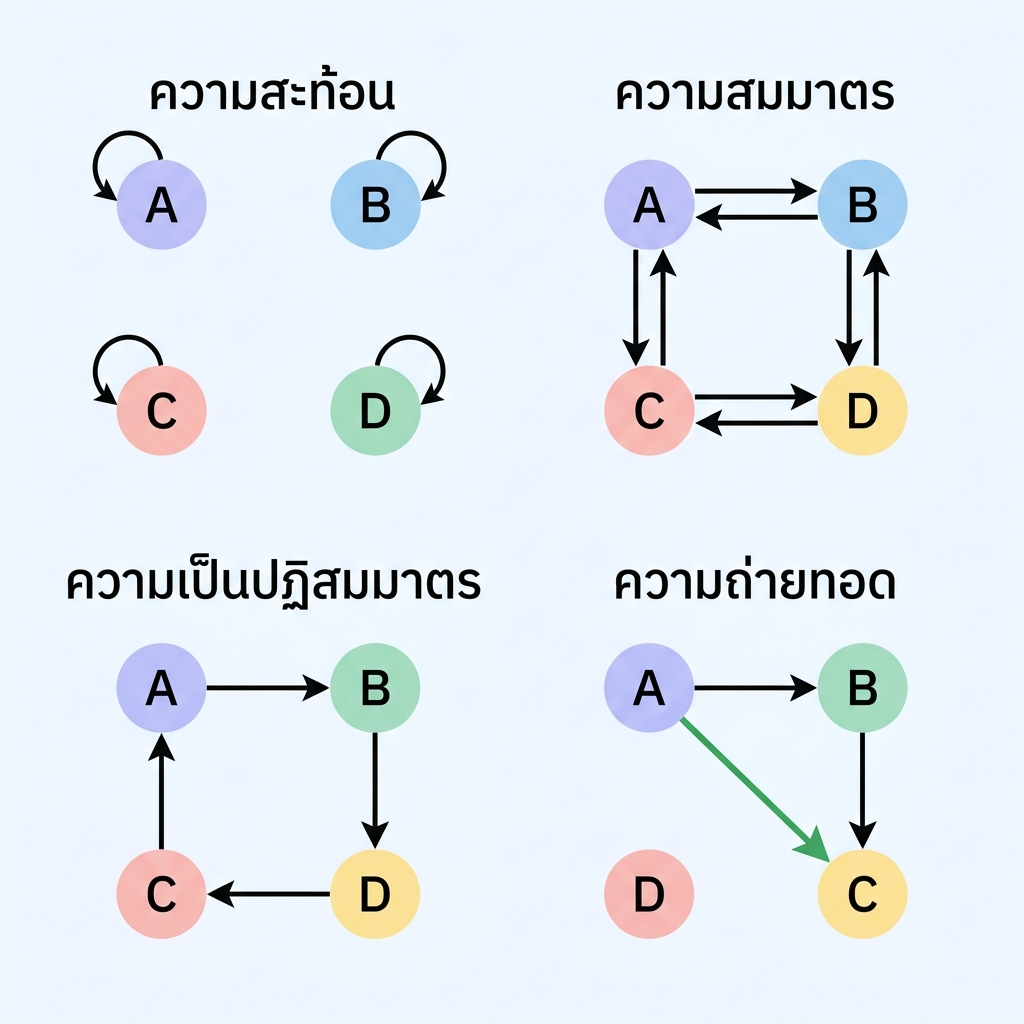
\includegraphics[width=0.68\textwidth]{Figures/png_ready/relation-properties-thai.png}
    \caption{คุณสมบัติ 4 ประการของความสัมพันธ์ทวิภาค}
    \label{fig:relation-properties-thai}
\end{figure}

\begin{ex}
\label{ex:relation-properties-check}
กำหนด $A = \{1, 2, 3\}$ และ $R_1 = \{(1,1), (2,2), (3,3), (1,2), (2,1)\}$ จงพิจารณาคุณสมบัติทั้ง 4 ประการ
\end{ex}
\begin{solution}
\begin{align*}
\text{สะท้อน} &\quad (1,1),(2,2),(3,3) \in R_1 \text{ ครบทุก } a \in A \Rightarrow \text{เป็นสะท้อน}\\
\text{สมมาตร} &\quad (1,2) \in R_1 \Rightarrow (2,1) \in R_1 \text{ และคู่ที่เหลือเป็นคู่ } (a,a) \Rightarrow \text{เป็นสมมาตร}\\
\text{ปฏิสมมาตร} &\quad (1,2),(2,1) \in R_1 \text{ แต่ } 1 \neq 2 \Rightarrow \text{ไม่เป็นปฏิสมมาตร}\\
\text{ถ่ายทอด} &\quad (1,2),(2,1) \Rightarrow (1,1) \in R_1 \text{ และ } (2,1),(1,2) \Rightarrow (2,2) \in R_1\\
&\quad \text{ส่วนคู่ที่เหลือมี } (a,a) \text{ เป็นสมาชิกหนึ่งจึงเป็นจริงเสมอ} \Rightarrow \text{เป็นถ่ายทอด}
\end{align*}
$\therefore R_1$ มีคุณสมบัติสะท้อน สมมาตร และถ่ายทอด แต่ไม่เป็นปฏิสมมาตร \solhere
\end{solution}

\subsection{การประกอบความสัมพันธ์}
ในระบบฐานข้อมูลบุคลากร ความสัมพันธ์ $R$ อาจเชื่อมพนักงานแต่ละคนเข้ากับแผนกที่สังกัด ขณะที่ความสัมพันธ์ $S$ เชื่อมแผนกเข้ากับอาคารที่ตั้งสำนักงาน การตอบคำถามว่าพนักงานคนหนึ่งทำงานอยู่ในอาคารใดจึงต้องเชื่อมความสัมพันธ์ทั้งสองเข้าด้วยกันโดยอาศัยแผนกเป็นตัวกลาง การเชื่อมต่อในลักษณะนี้เรียกว่าการประกอบความสัมพันธ์ ซึ่งเป็นเครื่องมือสำหรับหาเส้นทางที่มีความยาวหลายขั้นในกราฟ และเป็นพื้นฐานของการปิดถ่ายทอดในหัวข้อถัดไป

\begin{definition}[การประกอบความสัมพันธ์]
\index{ความสัมพันธ์!การประกอบ}
ให้ $R \subseteq A \times B$ และ $S \subseteq B \times C$ การประกอบความสัมพันธ์ (Composition of Relations) ของ $R$ กับ $S$ เขียนแทนด้วย $S \circ R \subseteq A \times C$ นิยามโดย
\[ S \circ R = \{(a,c) \in A \times C \mid \exists b \in B,\ (a,b) \in R \land (b,c) \in S\} \]
สำหรับความสัมพันธ์ $R$ บนเซต $A$ นิยามกำลังของความสัมพันธ์โดย $R^1 = R$ และ $R^{n+1} = R \circ R^n$ เมื่อ $n \ge 1$
\end{definition}

สัญลักษณ์ $S \circ R$ อ่านว่า ทำ $R$ ก่อนแล้วจึงทำ $S$ ซึ่งเป็นลำดับเดียวกับการประกอบฟังก์ชัน $g \circ f$ ที่จะศึกษาใน~\autoref{sec:functions} การตีความในเชิงกราฟคือ $(a,c) \in S \circ R$ ก็ต่อเมื่อมีเส้นทางเดินจาก $a$ ไปยัง $c$ โดยผ่านจุดกลาง $b$ เพียงจุดเดียว ดังนั้น $R^n$ จึงรวบรวมคู่ของจุดที่เดินถึงกันได้ด้วยเส้นทางความยาว $n$ ขั้นพอดี

\begin{ex}
\label{ex:relation-composition}
กำหนด $A = \{1,2,3\}$ และความสัมพันธ์ $R = \{(1,2),(2,3)\}$ บน $A$ จงหา $R^2$ และ $R^3$
\end{ex}
\begin{solution}
\begin{align*}
R^2 = R \circ R &= \{(a,c) \mid \exists b,\ (a,b) \in R \land (b,c) \in R\}\\
&= \{(1,3)\} \quad ((1,2) \in R \text{ และ } (2,3) \in R)\\
R^3 = R \circ R^2 &= \{(a,c) \mid \exists b,\ (a,b) \in R^2 \land (b,c) \in R\}\\
&= \varnothing \quad (\text{ไม่มีคู่อันดับใน } R \text{ ที่เริ่มต้นด้วย } 3)
\end{align*}
$\therefore R^2 = \{(1,3)\}$ และ $R^3 = \varnothing$ \solhere
\end{solution}

\subsection{การขยายและการปิดคุณสมบัติ}
ในการวิเคราะห์โครงสร้างความสัมพันธ์ ความสัมพันธ์เดิม $R$ อาจยังขาดคุณสมบัติบางประการที่จำเป็นต่อการประมวลผล การปิดคุณสมบัติ (Closure) เป็นกระบวนการขยายเซตความสัมพันธ์โดยเติมคู่อันดับเพิ่มเข้าไปใน $R$ ให้มีจำนวนน้อยที่สุด เพื่อสร้างความสัมพันธ์ใหม่ $R'$ ที่มีคุณสมบัติที่ต้องการอย่างสมบูรณ์ เช่น การปิดถ่ายทอด $t(R)$ ที่ใช้รวบรวมเส้นทางเชื่อมต่อทั้งหมดในทฤษฎีกราฟ โดยการปิดคุณสมบัติที่สำคัญ ได้แก่
\begin{enumerate}[label=\textbf{\arabic*.}]
    \item การปิดสะท้อน คือ $r(R) = R \cup \{(a,a) \mid a \in A\}$ ซึ่งเติมคู่อันดับที่จับคู่สมาชิกกับตัวเองให้ครบทุกตัว
    \item การปิดสมมาตร คือ $s(R) = R \cup R^{-1}$ ซึ่งเติมคู่อันดับทิศทางย้อนกลับให้ครบทุกคู่
    \item การปิดถ่ายทอด คือ $t(R) = R \cup R^2 \cup R^3 \cup \dots = \bigcup_{i=1}^{n} R^i$ ซึ่งรวบรวมเส้นทางเชื่อมต่อทุกความยาวเข้าไว้ด้วยกัน
\end{enumerate}

\begin{ex}
กำหนด $A = \{1, 2, 3\}$ และ $R = \{(1,2), (2,3)\}$ จงหา $r(R), s(R),$ และ $t(R)$
\end{ex}
\begin{solution}
\begin{align*}
r(R) &= R \cup \{(1,1), (2,2), (3,3)\} = \{(1,1),(2,2),(3,3),(1,2),(2,3)\}\\
s(R) &= R \cup R^{-1} = \{(1,2),(2,3),(2,1),(3,2)\}\\
t(R) &= R \cup R^2 = \{(1,2),(2,3),(1,3)\} \quad (\text{เพิ่มเส้นทางตรง } 1 \to 3)
\end{align*}
\solhere
\end{solution}

\begin{ex}
\label{ex:equivalence-relation-proof}
กำหนดความสัมพันธ์ $R$ บนเซตของจำนวนเต็ม $\mathbb{Z}$ โดย $a\,R\,b \iff a \equiv b \pmod 3$ (นั่นคือ $3$ หาร $a - b$ ลงตัว) จงพิสูจน์ว่า $R$ มีคุณสมบัติสะท้อน สมมาตร และถ่ายทอด
\end{ex}
\begin{solution}
\begin{align*}
\text{สะท้อน} &\quad a - a = 0 = 3(0) \Rightarrow a \equiv a \pmod 3 \Rightarrow (a,a) \in R \text{ สำหรับทุก } a \in \mathbb{Z}\\
\text{สมมาตร} &\quad (a,b) \in R \Rightarrow a - b = 3k,\ k \in \mathbb{Z} \Rightarrow b - a = 3(-k) \Rightarrow (b,a) \in R\\
\text{ถ่ายทอด} &\quad (a,b),(b,c) \in R \Rightarrow a - b = 3k,\ b - c = 3m\\
&\quad \Rightarrow a - c = (a-b) + (b-c) = 3(k+m) \Rightarrow (a,c) \in R
\end{align*}
$\therefore R$ มีคุณสมบัติสะท้อน สมมาตร และถ่ายทอดครบทั้งสามประการ \solhere
\end{solution}

\section{ฟังก์ชัน (Functions)}
\label{sec:functions}

เมื่อเข้าใจแนวคิดความสัมพันธ์แล้ว หัวข้อนี้จะพัฒนาต่อเข้าสู่เรื่องฟังก์ชัน ซึ่งเป็นความสัมพันธ์ชนิดพิเศษที่เพิ่มเงื่อนไขบังคับสองประการ ได้แก่ สมาชิกทุกตัวในเซตต้นทางต้องถูกจับคู่ และแต่ละตัวต้องจับคู่กับสมาชิกปลายทางเพียงตัวเดียว เงื่อนไขนี้ทำให้ฟังก์ชันมีพฤติกรรมที่คาดเดาได้ จึงเป็นแบบจำลองทางคณิตศาสตร์ของโปรแกรมย่อยที่รับข้อมูลเข้าชุดหนึ่งแล้วให้ผลลัพธ์ที่แน่นอนเสมอ หัวข้อนี้ครอบคลุมนิยามและองค์ประกอบของฟังก์ชัน การจำแนกประเภทตามลักษณะการจับคู่ การประกอบฟังก์ชันและฟังก์ชันผกผัน ตลอดจนฟังก์ชันพิเศษที่ใช้บ่อยในงานคอมพิวเตอร์

\subsection{นิยามฟังก์ชัน โดเมน โคโดเมน และเรนจ์}
ฟังก์ชัน $f: A \to B$ จัดเป็นความสัมพันธ์ชนิดพิเศษที่มีข้อจำกัดเชิงโครงสร้างอย่างรัดกุม โดยกำหนดให้สมาชิกทุกตัวในโดเมน $A$ ต้องจับคู่ไปยังสมาชิกในโคโดเมน $B$ เพียงตัวเดียวเท่านั้น ($f(a) = b$) นิยามการจับคู่ที่แน่นอนนี้ทำให้ฟังก์ชันเป็นเครื่องมือพื้นฐานในการอธิบายการส่งผ่านข้อมูล การแปลงพิกัด และการคำนวณในระบบคอมพิวเตอร์

\begin{definition}[ฟังก์ชัน]
\index{ฟังก์ชัน!นิยาม}
ให้ $A$ และ $B$ เป็นเซตที่ไม่เป็นเซตว่าง ฟังก์ชัน (Function) จาก $A$ ไปยัง $B$ เขียนแทนด้วยสัญลักษณ์ $f: A \to B$ คือความสัมพันธ์ $f \subseteq A \times B$ ซึ่งสำหรับทุกสมาชิก $a \in A$ จะต้องมีสมาชิก $b \in B$ เพียงตัวเดียวเท่านั้นที่ทำให้ $(a, b) \in f$ โดยเขียนแทนด้วยสมการ $f(a) = b$

องค์ประกอบหลักของฟังก์ชันมีดังนี้
\begin{enumerate}[label=\textbf{\arabic*.}]
    \item โดเมน (Domain) คือเซตต้นทางทั้งเซต นั่นคือ $\mathcal{D}(f) = A$
    \item โคโดเมน (Codomain) คือเซตของผลลัพธ์ที่เป็นไปได้ นั่นคือเซต $B$
    \item เรนจ์ (Range) คือเซตของผลลัพธ์ที่เกิดขึ้นจริง นั่นคือ $\mathcal{R}(f) = \{f(a) \in B \mid a \in A\} \subseteq B$
\end{enumerate}
\end{definition}

\begin{ex}
กำหนด $A=\{1,2,3\}$, $B=\{a,b,c\}$ จงตรวจสอบว่า $R_1=\{(1,a),(2,b),(3,b)\}$ และ $R_2=\{(1,a),(1,b),(2,c),(3,a)\}$ เป็นฟังก์ชันจาก $A$ ไป $B$ หรือไม่
\end{ex}
\begin{solution}
การพิจารณาความเป็นฟังก์ชัน ให้ตรวจสอบว่าสมาชิกแต่ละตัวในเซตต้นทาง $A$ ถูกใช้จับคู่เพียงครั้งเดียวหรือไม่
\begin{align*}
R_1 &= \{(1,a),(2,b),(3,b)\}\\
&\Rightarrow 1, 2, 3 \text{ จับคู่คนละหนึ่งครั้ง} \Rightarrow \text{เป็นฟังก์ชัน}\\
R_2 &= \{(1,a),(1,b),(2,c),(3,a)\}\\
&\Rightarrow 1 \text{ จับคู่ทั้ง } a \text{ และ } b \Rightarrow \text{ไม่เป็นฟังก์ชัน}
\end{align*}
$\therefore R_1$ เป็นฟังก์ชัน แต่ $R_2$ ไม่เป็นฟังก์ชัน \solhere
\end{solution}


\subsection{ฟังก์ชันหนึ่งต่อหนึ่ง ทั่วถึง และหนึ่งต่อหนึ่งทั่วถึง}
พิจารณาการจัดที่นั่งสำหรับนักศึกษาในห้องสอบ หากนักศึกษาทุกคนมีโต๊ะประจำตัวคนละ 1 ตัวพอดี และไม่มีโต๊ะว่างเหลืออยู่ จะสอดคล้องกับฟังก์ชันหนึ่งต่อหนึ่งทั่วถึง (Bijective) แต่หากมีนักศึกษาบางคนนั่งร่วมโต๊ะเดียวกัน หรือมีโต๊ะว่างเหลืออยู่ในห้องสอบ รูปแบบการจับคู่นั้นจะเปลี่ยนเป็นฟังก์ชันหนึ่งต่อหนึ่งหรือฟังก์ชันทั่วถึงตามเงื่อนไขที่กำหนด

\begin{definition}[ประเภทของฟังก์ชัน]
\index{ฟังก์ชัน!ประเภท}
ให้ $f:A \to B$ เป็นฟังก์ชัน
\begin{enumerate}[label=\textbf{\arabic*.}]
    \item ฟังก์ชันหนึ่งต่อหนึ่ง (Injective) คือฟังก์ชันที่ถ้า $f(a_1) = f(a_2)$ แล้ว $a_1 = a_2$
    \item ฟังก์ชันทั่วถึง (Surjective) คือฟังก์ชันที่สำหรับทุก $b \in B$ จะมี $a \in A$ ซึ่งทำให้ $f(a) = b$
    \item ฟังก์ชันหนึ่งต่อหนึ่งทั่วถึง (Bijective) คือฟังก์ชันที่เป็นทั้งหนึ่งต่อหนึ่งและทั่วถึง
\end{enumerate}
\end{definition}

ความแตกต่างของฟังก์ชันทั้งสามประเภทสังเกตได้จากรูปแบบของลูกศรที่ลากจากโดเมนไปยังโคโดเมน ฟังก์ชันหนึ่งต่อหนึ่งจะไม่มีสมาชิกใดในโคโดเมนที่รับลูกศรมากกว่าหนึ่งเส้น ฟังก์ชันทั่วถึงจะไม่มีสมาชิกใดในโคโดเมนที่ไม่ได้รับลูกศรเลย และฟังก์ชันหนึ่งต่อหนึ่งทั่วถึงจะมีลูกศรเข้าสู่สมาชิกทุกตัวของโคโดเมนพอดีหนึ่งเส้น ดังแสดงใน~\autoref{fig:function-types-thai}

\begin{figure}[H]
    \centering
    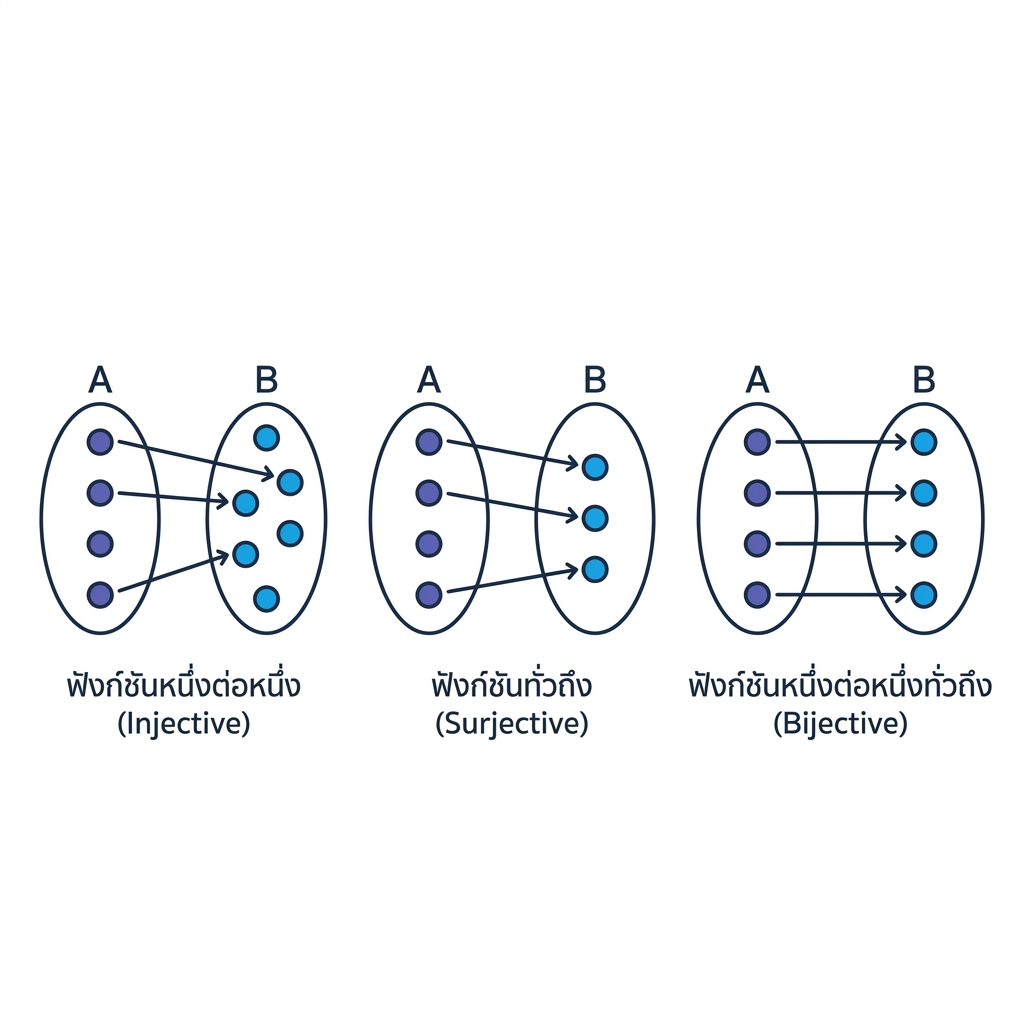
\includegraphics[width=0.68\textwidth]{Figures/png_ready/function-types-thai.png}
    \caption{แผนภาพเปรียบเทียบลักษณะการจับคู่ของฟังก์ชันหนึ่งต่อหนึ่ง ฟังก์ชันทั่วถึง และฟังก์ชันหนึ่งต่อหนึ่งทั่วถึง}
    \label{fig:function-types-thai}
\end{figure}

\begin{ex}
\label{ex:proof-bijective-real}
จงพิสูจน์ว่าฟังก์ชัน $f:\mathbb{R} \to \mathbb{R}$ ที่นิยามโดย $f(x) = x^3 + 1$ เป็นฟังก์ชันหนึ่งต่อหนึ่งทั่วถึง (Bijective)
\end{ex}
\begin{solution}
\begin{align*}
\text{หนึ่งต่อหนึ่ง} &\quad f(x_1) = f(x_2) \Rightarrow x_1^3 + 1 = x_2^3 + 1 \Rightarrow x_1^3 = x_2^3 \Rightarrow x_1 = x_2\\
\text{ทั่วถึง} &\quad \text{ให้ } y \in \mathbb{R},\ x^3 + 1 = y \Rightarrow x = \sqrt[3]{y - 1} \in \mathbb{R} \Rightarrow f(x) = y
\end{align*}
$\therefore f$ เป็นทั้งฟังก์ชันหนึ่งต่อหนึ่งและฟังก์ชันทั่วถึง จึงเป็นฟังก์ชันหนึ่งต่อหนึ่งทั่วถึง \solhere
\end{solution}

\subsection{การประกอบฟังก์ชันและฟังก์ชันผกผัน}
การคำนวณราคาสินค้าชำระเงินในระบบพาณิชย์อิเล็กทรอนิกส์ ประกอบด้วยขั้นตอนการคำนวณราคาสินค้าหลังหักส่วนลด ($f$) แล้วนำราคานั้นไปคำนวณภาษีมูลค่าเพิ่ม 7\% ต่อ ($g$) การทำงานต่อเนื่องสองขั้นตอนเรียกว่า การประกอบฟังก์ชัน ($g \circ f$) ขณะที่ฟังก์ชันผกผันคือกระบวนการคำนวณย้อนกลับจากยอดเงินสุทธิในใบเสร็จเพื่อหาว่าราคาสินค้าตั้งต้นก่อนหักส่วนลดมีค่าเท่าใด

\begin{definition}[การประกอบฟังก์ชัน และ ฟังก์ชันผกผัน]
\index{การประกอบฟังก์ชัน!นิยาม}
\index{ฟังก์ชันผกผัน!นิยาม}
\begin{enumerate}[label=\textbf{\arabic*.}]
    \item การประกอบฟังก์ชัน $g \circ f$ สำหรับ $f:A \to B$ และ $g:B \to C$ นิยามโดย $(g \circ f)(a) = g(f(a))$
    \item ฟังก์ชันผกผัน $f^{-1}$ ของฟังก์ชันหนึ่งต่อหนึ่งทั่วถึง $f:A \to B$ คือฟังก์ชัน $f^{-1}:B \to A$ ซึ่ง $f^{-1}(b) = a \iff f(a) = b$
\end{enumerate}
\end{definition}

การประกอบฟังก์ชันเกิดขึ้นได้ก็ต่อเมื่อเรนจ์ของฟังก์ชันที่ทำก่อนอยู่ภายในโดเมนของฟังก์ชันที่ทำทีหลัง ผลลัพธ์ที่ได้จึงเป็นฟังก์ชันใหม่ที่รับข้อมูลจากเซต $A$ แล้วส่งออกไปยังเซต $C$ โดยตรง โดยมีเซต $B$ ทำหน้าที่เป็นสถานะกลางที่ผู้ใช้งานไม่จำเป็นต้องรับรู้ ดังแสดงใน~\autoref{fig:function-composition}

\begin{figure}[H]
    \centering
    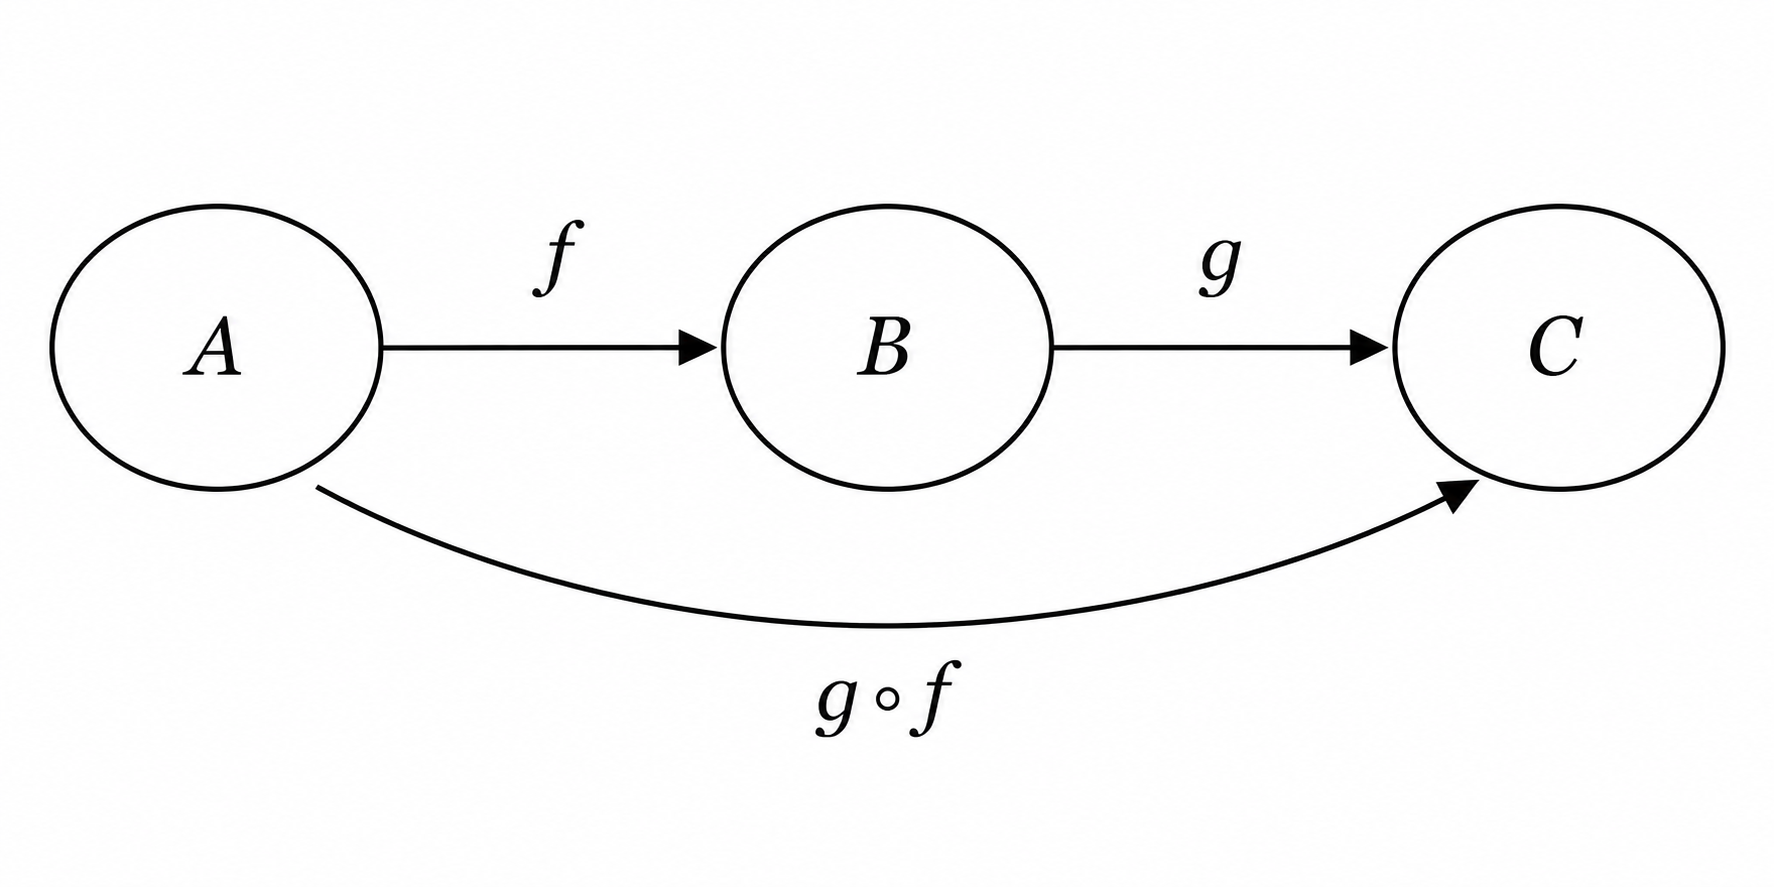
\includegraphics[width=0.62\textwidth]{Figures/png_ready/37-function-composition-manual.png}
    \caption{แผนภาพแสดงการประกอบฟังก์ชัน $(g \circ f)(a) = g(f(a))$ ที่ส่งผ่านข้อมูลจากเซต $A$ ผ่าน $B$ ไปยัง $C$}
    \label{fig:function-composition}
\end{figure}

\begin{ex}
ให้ $f(x)=2x+1$ บน $\mathbb{R}$ จงหา $(f \circ f)(x)$ และ $f^{-1}(x)$
\end{ex}
\begin{solution}
\begin{align*}
(f \circ f)(x) &= f(f(x)) = f(2x+1) = 2(2x+1)+1 = 4x+3\\
y = 2x+1 &\Rightarrow x = \frac{y-1}{2} \Rightarrow f^{-1}(x) = \frac{x-1}{2}
\end{align*}
$\therefore (f \circ f)(x) = 4x+3$ และ $f^{-1}(x) = \dfrac{x-1}{2}$ \solhere
\end{solution}

\begin{ex}
\label{ex:composition-inverse-two-func}
กำหนดฟังก์ชัน $f(x) = 3x - 4$ และ $g(x) = 2x + 5$ บน $\mathbb{R}$ จงหา $(g \circ f)(x)$ และ $(g \circ f)^{-1}(x)$
\end{ex}
\begin{solution}
\begin{align*}
(g \circ f)(x) &= g(f(x)) = g(3x-4) = 2(3x-4) + 5 = 6x - 8 + 5 = 6x - 3\\
y = 6x - 3 &\Rightarrow 6x = y + 3 \Rightarrow x = \frac{y+3}{6} \Rightarrow (g \circ f)^{-1}(x) = \frac{x+3}{6}
\end{align*}
$\therefore (g \circ f)(x) = 6x - 3$ และ $(g \circ f)^{-1}(x) = \dfrac{x+3}{6}$ \solhere
\end{solution}

\subsection{ฟังก์ชันพิเศษในทางคอมพิวเตอร์}
การประมวลผลข้อมูลในระบบคอมพิวเตอร์อาศัยการคำนวณรูปแบบเฉพาะ เช่น การจัดสรรยานพาหนะขนส่งผู้โดยสาร 45 คน โดยรถบัส 1 คันรองรับได้ 10 คน ระบบต้องปัดเศษขึ้นเป็น 5 คัน ($\lceil 45/10 \rceil = 5$) หรือการจัดลำดับการทำงานวนซ้ำทุก 7 วัน การดำเนินงานลักษณะนี้สอดคล้องกับฟังก์ชันพิเศษ ได้แก่ ฟังก์ชันปัดลง (Floor) ฟังก์ชันปัดขึ้น (Ceiling) และฟังก์ชันมอดูโล (Modulo)

\begin{definition}[ฟังก์ชันพิเศษ]
\index{ฟังก์ชันพิเศษ!Floor and Ceiling}
\index{ฟังก์ชันพิเศษ!Hash Function}
\begin{enumerate}[label=\textbf{\arabic*.}]
    \item ฟังก์ชันปัดลง (Floor) เขียนแทนด้วย $\lfloor x \rfloor$ คือจำนวนเต็มที่มากที่สุดซึ่งมีค่าน้อยกว่าหรือเท่ากับ $x$
    \item ฟังก์ชันปัดขึ้น (Ceiling) เขียนแทนด้วย $\lceil x \rceil$ คือจำนวนเต็มที่น้อยที่สุดซึ่งมีค่ามากกว่าหรือเท่ากับ $x$
    \item ฟังก์ชันมอดูโล (Modulo) เขียนแทนด้วย $x \bmod m$ คือเศษเหลือ $r$ ที่ทำให้ $x = qm + r$ โดยที่ $q \in \mathbb{Z}$ และ $0 \le r < m$ เมื่อ $m > 0$
    \item ฟังก์ชันแฮช (Hash Function) คือฟังก์ชัน $h: K \to S$ ที่แปลงคีย์ข้อมูลเป็นดรรชนีตำแหน่งจัดเก็บ เช่น $h(k) = k \bmod m$
\end{enumerate}
\end{definition}

นิยามของฟังก์ชันมอดูโลข้างต้นบังคับให้เศษเหลืออยู่ในช่วง $0 \le r < m$ เสมอ ผลลัพธ์ของตัวตั้งที่เป็นจำนวนลบจึงยังคงเป็นจำนวนไม่ติดลบ เช่น $-15 \bmod 4 = 1$ ข้อควรระวังในทางปฏิบัติคือภาษาโปรแกรมไม่ได้ใช้นิยามนี้ทั้งหมด ภาษา Python และ Ruby ให้ผลลัพธ์ตรงกับนิยามทางคณิตศาสตร์ ขณะที่ภาษา C, C++, Java และ JavaScript ใช้การหารแบบตัดเศษเข้าหาศูนย์ ทำให้ตัวดำเนินการ \texttt{\%} คืนค่า $-3$ สำหรับนิพจน์เดียวกัน ผู้เขียนโปรแกรมที่ต้องการผลลัพธ์ไม่ติดลบในภาษากลุ่มหลังจึงต้องเขียนเป็น \texttt{((x \% m) + m) \% m}

\begin{ex}
\label{ex:special-functions-calc}
จงคำนวณค่าของฟังก์ชันพิเศษต่อไปนี้
\begin{enumerate}[label=\textbf{\arabic*.}]
    \item $\lfloor 3.8 \rfloor$ และ $\lfloor -2.3 \rfloor$
    \item $\lceil 3.1 \rceil$ และ $\lceil -2.8 \rceil$
    \item $27 \bmod 6$ และ $-15 \bmod 4$
    \item ค่าแฮช $h(108)$ สำหรับฟังก์ชันแฮช $h(k) = k \bmod 11$
\end{enumerate}
\end{ex}
\begin{solution}
\begin{align*}
\lfloor 3.8 \rfloor &= 3, \qquad \lfloor -2.3 \rfloor = -3\\
\lceil 3.1 \rceil &= 4, \qquad \lceil -2.8 \rceil = -2\\
27 \bmod 6 &= 3 \quad (27 = 4 \times 6 + 3)\\
-15 \bmod 4 &= 1 \quad (-15 = -4 \times 4 + 1)\\
h(108) &= 108 \bmod 11 = 9 \quad (108 = 9 \times 11 + 9)
\end{align*}
\solhere
\end{solution}

\section{ลำดับและอนุกรม (Sequences and Series)}
\label{sec:sequences-and-series}

ในทางคณิตศาสตร์และคอมพิวเตอร์ ลำดับ (Sequence) คือฟังก์ชันที่มีโดเมนเป็นเซตของจำนวนเต็มบวก $\mathbb{Z}^+$ เขียนแทนด้วย $a: \mathbb{Z}^+ \to S$ หรือ $a_n = a(n)$ และเมื่อนำพจน์ในลำดับมาบวกสะสมกันจะเรียกว่า อนุกรม (Series) ซึ่งสอดคล้องกับพฤติกรรมการทำงานของวนลูป (Loop) และการวิเคราะห์ประสิทธิภาพของอัลกอริทึม

\subsection{ลำดับเลขคณิต (Arithmetic Sequence)}
พิจารณาการออมเงินโดยเริ่มต้นฝากเงินวันแรก 10 บาท และเพิ่มเงินฝากขึ้นวันละ 5 บาทอย่างสม่ำเสมอ จำนวนเงินฝากในแต่ละวันจะเป็น 10, 15, 20, 25,... ซึ่งเรียงลำดับเป็นลำดับเลขคณิต การคำนวณเงินฝาก ณ วันที่ 30 คือการหาพจน์ของลำดับ ส่วนการคำนวณเงินออมสะสมรวมทั้งหมดตั้งแต่วันแรกถึงวันที่ 30 คือการคำนวณผลรวมอนุกรมเลขคณิต

\begin{definition}[ลำดับเลขคณิต]
\index{ลำดับ!เลขคณิต}
ลำดับเลขคณิต (Arithmetic Sequence) คือลำดับที่ผลต่างของพจน์ที่อยู่ติดกันมีค่าคงตัว เรียกว่า ผลต่างร่วม (Common Difference) เขียนแทนด้วย $d = a_{n+1} - a_n$ โดยมีพจน์ทั่วไป (General Term) นิยามโดย
\[ a_n = a_1 + (n-1)d \]
เมื่อ $a_1$ คือพจน์แรก และ $n$ คือลำดับพจน์ที่ต้องการคำนวณ
\end{definition}

\begin{ex}
กำหนดลำดับเลขคณิต $3, 7, 11, 15, \dots$ จงหาผลต่างร่วม $d$ และพจน์ที่ 20 ($a_{20}$)
\end{ex}
\begin{solution}
\begin{align*}
a_1 &= 3, \quad d = 7 - 3 = 4\\
a_{20} &= a_1 + (20-1)d = 3 + (19)(4) = 3 + 76 = 79
\end{align*}
$\therefore d = 4$ และ $a_{20} = 79$ \solhere
\end{solution}

\begin{ex}
\label{ex:arithmetic-sequence-find-n}
กำหนดลำดับเลขคณิต $7, 11, 15, 19, \dots, 83$ จงหาว่าลำดับนี้มีทั้งหมดกี่พจน์
\end{ex}
\begin{solution}
\begin{align*}
a_1 &= 7, \quad d = 11 - 7 = 4, \quad a_n = 83\\
83 &= 7 + (n-1)4\\
76 &= (n-1)4\\
n - 1 &= 19 \ \Rightarrow \ n = 20
\end{align*}
$\therefore$ ลำดับนี้มีทั้งหมด 20 พจน์ \solhere
\end{solution}

\subsection{ลำดับเรขาคณิต (Geometric Sequence)}
พิจารณาการแพร่กระจายข้อมูลในเครือข่ายสังคม หากบุคคล 1 คนส่งต่อข้อมูลให้ผู้รับ 2 คน จากนั้นผู้รับทั้ง 2 คนนำไปส่งต่อให้ผู้รับรายใหม่คนละ 2 คน จำนวนผู้รับข้อมูลจะเพิ่มขึ้นเป็น 4, 8, 16 คนตามลำดับ การเพิ่มขึ้นในลักษณะทวีคูณนี้คือ ลำดับเรขาคณิต และการคำนวณจำนวนผู้ได้รับข้อมูลทั้งหมดในระบบคือ อนุกรมเรขาคณิต

\begin{definition}[ลำดับเรขาคณิต]
\index{ลำดับ!เรขาคณิต}
ลำดับเรขาคณิต (Geometric Sequence) คือลำดับที่อัตราส่วนของพจน์ที่อยู่ติดกันมีค่าคงตัว เรียกว่า อัตราส่วนร่วม (Common Ratio) เขียนแทนด้วย $r = \frac{a_{n+1}}{a_n}$ โดยมีพจน์ทั่วไปนิยามโดย
\[ a_n = a_1 r^{n-1} \]
เมื่อ $a_1$ คือพจน์แรก และ $r \neq 0$ คืออัตราส่วนร่วม
\end{definition}

\begin{ex}
กำหนดลำดับเรขาคณิต $2, 6, 18, 54, \dots$ จงหาอัตราส่วนร่วม $r$ และพจน์ที่ 7 ($a_7$)
\end{ex}
\begin{solution}
\begin{align*}
a_1 &= 2, \quad r = \frac{6}{2} = 3\\
a_7 &= a_1 r^{7-1} = 2 \times 3^6 = 2 \times 729 = 1458
\end{align*}
$\therefore r = 3$ และ $a_7 = 1458$ \solhere
\end{solution}

\subsection{อนุกรมเลขคณิต (Arithmetic Series)}
การหาผลรวมสะสมของข้อมูลในลำดับเลขคณิตตั้งแต่พจน์แรกจนถึงพจน์ที่ต้องการ เรียกว่า อนุกรมเลขคณิต ในทางคอมพิวเตอร์ การคำนวณผลรวมนี้สอดคล้องกับการหาจำนวนรอบการทำงานรวมของวนลูปซ้อน (Nested Loop) ที่มีจำนวนรอบเปลี่ยนไปอย่างเป็นรูปธรรม

\begin{definition}[อนุกรมเลขคณิต]
\index{อนุกรม!เลขคณิต}
อนุกรมเลขคณิต (Arithmetic Series) คือผลรวมของพจน์ในลำดับเลขคณิต เขียนแทนด้วย $S_n = \sum_{i=1}^{n} a_i$ โดยมีสูตรคำนวณผลรวม $n$ พจน์แรกดังนี้
\[ S_n = \frac{n(a_1 + a_n)}{2} = \frac{n[2a_1 + (n-1)d]}{2} \]
\end{definition}

\begin{ex}
จงหาผลรวม 10 พจน์แรก ($S_{10}$) ของอนุกรมเลขคณิต $5 + 8 + 11 + 14 + \dots$
\end{ex}
\begin{solution}
\begin{align*}
a_1 &= 5, \quad d = 8 - 5 = 3, \quad n = 10\\
S_{10} &= \frac{n[2a_1 + (n-1)d]}{2} = \frac{10[2(5) + 9(3)]}{2}\\
&= 5[10 + 27] = 5 \times 37 = 185
\end{align*}
$\therefore$ ผลรวม 10 พจน์แรก $S_{10} = 185$ \solhere
\end{solution}

\subsection{อนุกรมเรขาคณิต (Geometric Series)}
ในการวิเคราะห์ประสิทธิภาพของอัลกอริทึมแบบแบ่งแยกและเอาชนะ (Divide and Conquer) ผลรวมของภาระงานในทุกระดับชั้นของโครงสร้างการประมวลผลสามารถเขียนแทนได้ด้วยอนุกรมเรขาคณิต สูตรคำนวณผลรวมอนุกรมเรขาคณิตจึงช่วยให้ประเมินขอบเขตเวลาการทำงานรวมของโปรแกรมได้อย่างรวดเร็ว

\begin{definition}[อนุกรมเรขาคณิต]
\index{อนุกรม!เรขาคณิต}
อนุกรมเรขาคณิต (Geometric Series) คือผลรวมของพจน์ในลำดับเรขาคณิต เขียนแทนด้วย $S_n = \sum_{i=1}^{n} a_1 r^{i-1}$ โดยมีสูตรคำนวณผลรวม $n$ พจน์แรกดังนี้
\[ S_n = \frac{a_1(r^n - 1)}{r - 1} = \frac{a_1(1 - r^n)}{1 - r} \quad (\text{เมื่อ } r \neq 1) \qquad S_n = n a_1 \quad (\text{เมื่อ } r = 1) \]
และเมื่อ $\lvert r \rvert < 1$ ผลรวมของพจน์ทั้งหมดอย่างไม่จำกัดจำนวนจะลู่เข้าสู่ค่าจำกัด เรียกว่าผลรวมอนันต์ (Infinite Sum) นิยามโดย
\[ S_\infty = \sum_{i=1}^{\infty} a_1 r^{i-1} = \frac{a_1}{1 - r} \]
\end{definition}

สูตรทั้งสองรูปของ $S_n$ เมื่อ $r \neq 1$ มีค่าเท่ากันเสมอ เพราะเกิดจากการคูณทั้งเศษและส่วนด้วย $-1$ การเลือกใช้รูปใดจึงเป็นเพียงความสะดวกในการคำนวณ โดยนิยมใช้รูปแรกเมื่อ $r > 1$ เพื่อให้ตัวส่วนเป็นบวก และใช้รูปที่สองเมื่อ $r < 1$ ด้วยเหตุผลเดียวกัน ส่วนกรณี $r = 1$ ต้องแยกพิจารณาต่างหาก เนื่องจากตัวส่วน $r - 1$ มีค่าเป็นศูนย์ ซึ่งในกรณีนี้ทุกพจน์มีค่าเท่ากับ $a_1$ ผลรวมจึงเท่ากับ $n a_1$

\begin{ex}
จงหาผลรวม 6 พจน์แรก ($S_6$) ของอนุกรมเรขาคณิต $3 + 6 + 12 + 24 + \dots$
\end{ex}
\begin{solution}
\begin{align*}
a_1 &= 3, \quad r = \frac{6}{3} = 2, \quad n = 6\\
S_6 &= \frac{a_1(r^n - 1)}{r - 1} = \frac{3(2^6 - 1)}{2 - 1} = \frac{3(64-1)}{1} = 3 \times 63 = 189
\end{align*}
$\therefore$ ผลรวม 6 พจน์แรก $S_6 = 189$ \solhere
\end{solution}

\begin{ex}
\label{ex:infinite-geometric-series}
จงหาผลรวมอนันต์ ($S_\infty$) ของอนุกรมเรขาคณิต $12 + 6 + 3 + 1.5 + \dots$
\end{ex}
\begin{solution}
\begin{align*}
a_1 &= 12, \quad r = \frac{6}{12} = \frac{1}{2} \quad (\lvert r \rvert < 1 \text{ อนุกรมจึงลู่เข้า})\\
S_\infty &= \frac{a_1}{1 - r} = \frac{12}{1 - \tfrac{1}{2}} = \frac{12}{\tfrac{1}{2}} = 24
\end{align*}
$\therefore$ ผลรวมอนันต์ $S_\infty = 24$ \solhere
\end{solution}

\section{การประยุกต์ใช้ในวิทยาการคอมพิวเตอร์}
\label{sec:relation-applications}

แนวคิดเรื่องความสัมพันธ์ ฟังก์ชัน ลำดับ และอนุกรม ถูกนำไปใช้เป็นแกนหลักในการออกแบบซอฟต์แวร์และโครงสร้างข้อมูลทางคอมพิวเตอร์ หัวข้อนี้ยกตัวอย่างการประยุกต์ใช้ในสามบริบทที่นักศึกษาจะพบในรายวิชาถัดไป ได้แก่ การจัดเก็บข้อมูลเชิงตารางในระบบฐานข้อมูล การกำหนดลำดับการทำงานของคำสั่งในตัวแปลภาษา และการจัดสรรตำแหน่งจัดเก็บข้อมูลในตารางแฮช ทั้งสามบริบทอาศัยแนวคิดเดียวกันคือการมองการจับคู่ระหว่างข้อมูลเป็นเซตของคู่อันดับที่มีสมบัติทางคณิตศาสตร์กำกับ

\subsection{ฐานข้อมูลเชิงสัมพันธ์และพีชคณิตเชิงสัมพันธ์}
แบบจำลองฐานข้อมูลเชิงสัมพันธ์ (Relational Model) ที่เอ็ดการ์ คอดด์ เสนอไว้ในปี ค.ศ. 1970 มองตารางข้อมูลหนึ่งตารางเป็นความสัมพันธ์ทางคณิตศาสตร์ $R \subseteq A_1 \times A_2 \times \dots \times A_n$ เมื่อ $A_i$ คือเซตของค่าที่คอลัมน์ที่ $i$ รับได้~\cite{codd1970relational} แต่ละแถวของตารางคือทูเปิล (Tuple) ซึ่งก็คือสมาชิกหนึ่งตัวของความสัมพันธ์ ส่วนแต่ละคอลัมน์คือแอตทริบิวต์ (Attribute) ซึ่งกำหนดความหมายของค่าในตำแหน่งนั้น การมองตารางเป็นเซตทำให้การสืบค้นข้อมูลกลายเป็นการดำเนินการบนเซตที่มีนิยามทางคณิตศาสตร์รองรับ เรียกว่าพีชคณิตเชิงสัมพันธ์ (Relational Algebra)

การดำเนินการพื้นฐานของพีชคณิตเชิงสัมพันธ์สอดคล้องโดยตรงกับการดำเนินการบนเซตที่ศึกษามาแล้ว การเลือก (Selection) เขียนแทนด้วย $\sigma_{\varphi}(R)$ คือการคัดเฉพาะทูเปิลที่ทำให้เงื่อนไข $\varphi$ เป็นจริง ซึ่งก็คือการสร้างเซตย่อยของ $R$ การฉาย (Projection) เขียนแทนด้วย $\pi_{A_i}(R)$ คือการเลือกเฉพาะบางแอตทริบิวต์ ซึ่งให้ผลเป็นเรนจ์ของความสัมพันธ์เมื่อพิจารณาเฉพาะคอลัมน์ที่สนใจ และการเชื่อมตามธรรมชาติ (Natural Join) เขียนแทนด้วย $R \bowtie S$ คือการจับคู่ทูเปิลจากสองตารางที่มีค่าตรงกันในแอตทริบิวต์ร่วม ซึ่งเป็นรูปแบบหนึ่งของการประกอบความสัมพันธ์ที่ศึกษาใน~\autoref{sec:relation-properties}

\subsection{การจัดลำดับการทำงานของโปรแกรม}
ในตัวแปลภาษา การวิเคราะห์ไวยากรณ์ (Parsing) ต้องตรวจสอบว่าวงเล็บเปิดและวงเล็บปิดในนิพจน์จับคู่กันครบถ้วนหรือไม่ กระบวนการนี้อาศัยฟังก์ชันที่ส่งนิพจน์ไปยังค่าความจริงว่าสมดุลหรือไม่สมดุล โดยใช้โครงสร้างข้อมูลกองซ้อน (Stack) เก็บวงเล็บเปิดที่ยังไม่ถูกจับคู่ นิพจน์จะสมดุลก็ต่อเมื่ออ่านจนจบแล้วกองซ้อนว่างเปล่าพอดี

การจัดลำดับการทำงานของคำสั่งที่ต้องประมวลผลตามลำดับก่อนหลังใช้ความสัมพันธ์ $R = \{(s_1, s_2) \mid s_1 \text{ ต้องทำงานเสร็จก่อน } s_2\}$ ซึ่งต้องมีคุณสมบัติปฏิสมมาตรและถ่ายทอด หากความสัมพันธ์นี้เกิดวงจรปิด เช่น คำสั่ง $s_1$ ต้องรอ $s_2$ ขณะที่ $s_2$ ก็ต้องรอ $s_1$ ระบบจะเข้าสู่ภาวะติดตาย (Deadlock) และไม่มีคำสั่งใดทำงานต่อได้ การตรวจสอบว่าความสัมพันธ์ปลอดวงจรปิดจึงทำได้โดยคำนวณการปิดถ่ายทอด $t(R)$ แล้วตรวจว่ามีคู่อันดับในรูป $(s,s)$ ปรากฏขึ้นหรือไม่

\subsection{การจัดเก็บข้อมูลด้วยตารางแฮชและการแก้ปัญหาการชนกัน}
ตารางแฮช (Hash Table) ใช้ฟังก์ชันแฮชแปลงคีย์ข้อมูลให้เป็นดรรชนีตำแหน่งจัดเก็บโดยตรง จึงเข้าถึงข้อมูลได้โดยไม่ต้องค้นหาทีละตำแหน่ง อย่างไรก็ตาม ฟังก์ชันแฮชโดยทั่วไปไม่ใช่ฟังก์ชันหนึ่งต่อหนึ่ง เพราะจำนวนคีย์ที่เป็นไปได้มักมากกว่าจำนวนช่องในตาราง เมื่อคีย์ต่างกันสองตัวถูกส่งไปยังดรรชนีเดียวกันจะเรียกว่าการชนกัน (Collision) วิธีแก้ปัญหาที่ตรงไปตรงมาที่สุดคือการสำรวจเชิงเส้น (Linear Probing) ซึ่งเลื่อนไปตรวจช่องถัดไปทีละหนึ่งตำแหน่งจนกว่าจะพบช่องว่าง

\begin{ex}
\label{ex:hash-table-linear-probing}
กำหนดฟังก์ชันแฮช $h(k) = k \bmod 7$ และชุดคีย์ $K = \{12, 19, 26, 33\}$ จงหาดรรชนีแฮช และแสดงการจัดเก็บข้อมูลด้วย Linear Probing เมื่อเกิดการชนกัน
\end{ex}
\begin{solution}
\begin{align*}
h(12) &= 12 \bmod 7 = 5 &&\Rightarrow \text{ช่องว่าง เก็บ } 12 \text{ ที่ดรรชนี } 5\\
h(19) &= 19 \bmod 7 = 5 &&\Rightarrow \text{ชนกัน}, \ (5+1) \bmod 7 = 6 \Rightarrow \text{เก็บ } 19 \text{ ที่ดรรชนี } 6\\
h(26) &= 26 \bmod 7 = 5 &&\Rightarrow \text{ชนกัน}, \ (5+2) \bmod 7 = 0 \Rightarrow \text{เก็บ } 26 \text{ ที่ดรรชนี } 0\\
h(33) &= 33 \bmod 7 = 5 &&\Rightarrow \text{ชนกัน}, \ (5+3) \bmod 7 = 1 \Rightarrow \text{เก็บ } 33 \text{ ที่ดรรชนี } 1
\end{align*}
$\therefore$ ตารางแฮชจัดเก็บข้อมูลที่ดรรชนี 0, 1, 5 และ 6 ด้วยคีย์ 26, 33, 12 และ 19 ตามลำดับ \solhere
\end{solution}

\sectionbanner{สรุปบทเรียน}
ความสัมพันธ์และฟังก์ชันเป็นรากฐานทางคณิตศาสตร์ที่สำคัญของโครงสร้างข้อมูลและการประมวลผลทางคอมพิวเตอร์ ความสัมพันธ์ $R \subseteq A \times B$ อธิบายการจับคู่ระหว่างสมาชิกสองเซต ความสัมพันธ์ทวิภาคบนเซตเดียวกันจำแนกตามคุณสมบัติสะท้อน สมมาตร ปฏิสมมาตร และถ่ายทอด รวมถึงการปิดคุณสมบัติสะท้อน สมมาตร และถ่ายทอดเพื่อวิเคราะห์การเชื่อมต่อในทฤษฎีกราฟ

ฟังก์ชัน $f: A \to B$ จัดเป็นความสัมพันธ์ชนิดพิเศษที่สมาชิกต้นทางทุกตัวถูกจับคู่ไปยังสมาชิกปลายทางเพียงตัวเดียว จำแนกเป็นฟังก์ชันหนึ่งต่อหนึ่ง ทั่วถึง และหนึ่งต่อหนึ่งทั่วถึง ซึ่งรองรับการประกอบฟังก์ชัน $(g \circ f)$ ฟังก์ชันผกผัน $f^{-1}$ รวมถึงฟังก์ชันพิเศษในทางคอมพิวเตอร์ ได้แก่ ฟังก์ชันปัดลง ฟังก์ชันปัดขึ้น ฟังก์ชันมอดูโล และฟังก์ชันแฮช

นอกจากนี้ การศึกษายังครอบคลุมถึงลำดับและอนุกรม ได้แก่ ลำดับเลขคณิต ($a_n = a_1 + (n-1)d$), ลำดับเรขาคณิต ($a_n = a_1 r^{n-1}$), อนุกรมเลขคณิต ($S_n = \frac{n(a_1+a_n)}{2}$) และอนุกรมเรขาคณิต ($S_n = \frac{a_1(r^n-1)}{r-1}$) ซึ่งเป็นแกนหลักของการคำนวณแบบวนลูปและการวิเคราะห์ประสิทธิภาพอัลกอริทึม ทั้งหมดนี้ได้รับการประยุกต์ใช้ในระบบฐานข้อมูลเชิงสัมพันธ์ การตรวจสอบไวยากรณ์คอมไพเลอร์ และการจัดลำดับการทำงานขนาน

\clearpage
\sectionbanner{แบบฝึกหัด}

\exercisepart{ส่วนที่ 1: ความสัมพันธ์และคู่อันดับ}
\begin{exercise}
กำหนดให้ $A = \{1, 2, 3\}$ และ $B = \{a, b\}$ จงหาสิ่งต่อไปนี้
\begin{enumerate}
    \item $A \times B$ และ $B \times A$
    \item จำนวนความสัมพันธ์ทั้งหมดที่เป็นไปได้จาก $A$ ไป $B$
    \item จำนวนความสัมพันธ์ทวิภาคทั้งหมดบนเซต $A$
\end{enumerate}
\end{exercise}

\begin{exercise}
กำหนด $A = \{1, 2, 3, 4\}$ และความสัมพันธ์ $R = \{(x,y) \in A \times A \mid x + y \le 5\}$ จงหาสิ่งต่อไปนี้
\begin{enumerate}
    \item สมาชิกทั้งหมดในความสัมพันธ์ $R$
    \item โดเมน $\mathcal{D}(R)$ และเรนจ์ $\mathcal{R}(R)$
    \item ความสัมพันธ์ผกผัน $R^{-1}$
\end{enumerate}
\end{exercise}

\exercisepart{ส่วนที่ 2: คุณสมบัติและการปิดคุณสมบัติของความสัมพันธ์}
\begin{exercise}
พิจารณาความสัมพันธ์ทวิภาคต่อไปนี้บนเซต $A = \{1, 2, 3, 4\}$ ว่ามีคุณสมบัติ สะท้อน, สมมาตร, ปฏิสมมาตร, หรือถ่ายทอด หรือไม่
\begin{enumerate}
    \item $R_1 = \{(1,1), (2,2), (3,3), (4,4)\}$
    \item $R_2 = \{(1,2), (2,1), (2,3), (3,2)\}$
    \item $R_3 = \{(1,1), (1,2), (2,2), (2,3), (1,3)\}$
    \item $R_4 = \{(1,2), (3,4)\}$
\end{enumerate}
\end{exercise}

\begin{exercise}
กำหนด $A = \{1, 2, 3\}$ และความสัมพันธ์ $R = \{(1,2), (2,3)\}$ จงหาสิ่งต่อไปนี้
\begin{enumerate}
    \item การปิดสะท้อน (Reflexive Closure) $r(R)$
    \item การปิดสมมาตร (Symmetric Closure) $s(R)$
    \item การปิดถ่ายทอด (Transitive Closure) $t(R)$
\end{enumerate}
\end{exercise}

\exercisepart{ส่วนที่ 3: นิยามและประเภทของฟังก์ชัน}
\begin{exercise}
พิจารณาว่าความสัมพันธ์ต่อไปนี้เป็นฟังก์ชันจาก $A = \{1, 2, 3\}$ ไปยัง $B = \{a, b, c\}$ หรือไม่ พร้อมระบุประเภทของฟังก์ชัน
\begin{enumerate}
    \item $f_1 = \{(1,a), (2,b), (3,c)\}$
    \item $f_2 = \{(1,a), (2,a), (3,b)\}$
    \item $f_3 = \{(1,a), (1,b), (2,c), (3,a)\}$
    \item $f_4 = \{(1,b), (2,c), (3,a)\}$
\end{enumerate}
\end{exercise}

\begin{exercise}
กำหนดฟังก์ชัน $f(x) = 3x - 5$ บนเซตของจำนวนจริง $\mathbb{R}$
\begin{enumerate}
    \item จงพิสูจน์ว่า $f$ เป็นฟังก์ชันหนึ่งต่อหนึ่ง (Injective)
    \item จงพิสูจน์ว่า $f$ เป็นฟังก์ชันทั่วถึง (Surjective)
    \item จงหาฟังก์ชันผกผัน $f^{-1}(x)$
\end{enumerate}
\end{exercise}

\exercisepart{ส่วนที่ 4: การประกอบฟังก์ชันและฟังก์ชันพิเศษ}
\begin{exercise}
กำหนด $f(x) = 2x + 3$ และ $g(x) = x^2 - 1$ บน $\mathbb{R}$ จงหาสิ่งต่อไปนี้
\begin{enumerate}
    \item $(g \circ f)(x)$ และ $(g \circ f)(2)$
    \item $(f \circ g)(x)$ และ $(f \circ g)(2)$
    \item $(f \circ f)(x)$
\end{enumerate}
\end{exercise}

\begin{exercise}
จงคำนวณค่าของฟังก์ชันพิเศษต่อไปนี้
\begin{enumerate}
    \item $\lfloor 4.8 \rfloor$ และ $\lfloor -3.2 \rfloor$
    \item $\lceil 2.1 \rceil$ และ $\lceil -1.7 \rceil$
    \item $37 \bmod 5$ และ $-14 \bmod 4$
    \item ค่าแฮช $h(k) = k \bmod 11$ เมื่อ $k = 125$
\end{enumerate}
\end{exercise}

\exercisepart{ส่วนที่ 5: ลำดับและอนุกรม}
\begin{exercise}
กำหนดลำดับเลขคณิต $4, 9, 14, 19, \dots$ จงหาสิ่งต่อไปนี้
\begin{enumerate}
    \item ผลต่างร่วม $d$ และพจน์ทั่วไป $a_n$
    \item พจน์ที่ 15 ($a_{15}$)
    \item ผลรวม 15 พจน์แรก ($S_{15}$)
\end{enumerate}
\end{exercise}

\begin{exercise}
กำหนดลำดับเรขาคณิต $3, 6, 12, 24, \dots$ จงหาสิ่งต่อไปนี้
\begin{enumerate}
    \item อัตราส่วนร่วม $r$ และพจน์ทั่วไป $a_n$
    \item พจน์ที่ 8 ($a_8$)
    \item ผลรวม 8 พจน์แรก ($S_8$)
\end{enumerate}
\end{exercise}

\answerkeyhead
\exercisepart{เฉลยส่วนที่ 1: ความสัมพันธ์และคู่อันดับ}
\begin{enumerate}[label={},leftmargin=0pt,itemsep=0.6em]
    \item
    \begin{enumerate}[label=\textbf{\thechapter.\arabic{enumi}.\arabic*}]
        \item $A \times B = \{(1,a),(1,b),(2,a),(2,b),(3,a),(3,b)\}$, $B \times A = \{(a,1),(a,2),(a,3),(b,1),(b,2),(b,3)\}$
        \item $2^{|A \times B|} = 2^6 = 64$ ความสัมพันธ์
        \item $2^{|A \times A|} = 2^9 = 512$ ความสัมพันธ์
    \end{enumerate}

    \item
    \begin{enumerate}[label=\textbf{\thechapter.\arabic{enumi}.\arabic*}]
        \item $R = \{(1,1),(1,2),(1,3),(1,4),(2,1),(2,2),(2,3),(3,1),(3,2),(4,1)\}$
        \item $\mathcal{D}(R) = \{1,2,3,4\}$, $\mathcal{R}(R) = \{1,2,3,4\}$
        \item $R^{-1} = \{(1,1),(2,1),(3,1),(4,1),(1,2),(2,2),(3,2),(1,3),(2,3),(1,4)\}$
    \end{enumerate}
\end{enumerate}

\exercisepart{เฉลยส่วนที่ 2: คุณสมบัติและการปิดคุณสมบัติของความสัมพันธ์}
\begin{enumerate}[label={},leftmargin=0pt,itemsep=0.6em]
    \setcounter{enumi}{2}
    \item
    \begin{enumerate}[label=\textbf{\thechapter.\arabic{enumi}.\arabic*}]
        \item $R_1$ เป็นสะท้อน สมมาตร ปฏิสมมาตร และถ่ายทอด ครบทั้งสี่ประการ
        \item $R_2$ เป็นสมมาตรเท่านั้น ไม่สะท้อน ไม่เป็นปฏิสมมาตร และไม่ถ่ายทอด
        \item $R_3$ เป็นปฏิสมมาตรและถ่ายทอด แต่ไม่สะท้อน เพราะขาด $(3,3)$ และ $(4,4)$
        \item $R_4$ เป็นปฏิสมมาตรและถ่ายทอด
    \end{enumerate}

    \item
    \begin{enumerate}[label=\textbf{\thechapter.\arabic{enumi}.\arabic*}]
        \item $r(R) = \{(1,1),(2,2),(3,3),(1,2),(2,3)\}$
        \item $s(R) = \{(1,2),(2,3),(2,1),(3,2)\}$
        \item $t(R) = \{(1,2),(2,3),(1,3)\}$
    \end{enumerate}
\end{enumerate}

\exercisepart{เฉลยส่วนที่ 3: นิยามและประเภทของฟังก์ชัน}
\begin{enumerate}[label={},leftmargin=0pt,itemsep=0.6em]
    \setcounter{enumi}{4}
    \item
    \begin{enumerate}[label=\textbf{\thechapter.\arabic{enumi}.\arabic*}]
        \item $f_1$ เป็นฟังก์ชันหนึ่งต่อหนึ่งทั่วถึง
        \item $f_2$ เป็นฟังก์ชัน แต่ไม่เป็นหนึ่งต่อหนึ่งและไม่เป็นทั่วถึง
        \item $f_3$ ไม่เป็นฟังก์ชัน เพราะสมาชิก 1 จับคู่ซ้ำทั้ง $a$ และ $b$
        \item $f_4$ เป็นฟังก์ชันหนึ่งต่อหนึ่งทั่วถึง
    \end{enumerate}

    \item
    \begin{enumerate}[label=\textbf{\thechapter.\arabic{enumi}.\arabic*}]
        \item ให้ $f(x_1) = f(x_2) \implies 3x_1 - 5 = 3x_2 - 5 \implies x_1 = x_2$ (เป็น Injective)
        \item ให้ $y \in \mathbb{R} \implies 3x - 5 = y \implies x = \frac{y+5}{3} \in \mathbb{R}$ (เป็น Surjective)
        \item $f^{-1}(x) = \dfrac{x+5}{3}$
    \end{enumerate}
\end{enumerate}

\exercisepart{เฉลยส่วนที่ 4: การประกอบฟังก์ชันและฟังก์ชันพิเศษ}
\begin{enumerate}[label={},leftmargin=0pt,itemsep=0.6em]
    \setcounter{enumi}{6}
    \item
    \begin{enumerate}[label=\textbf{\thechapter.\arabic{enumi}.\arabic*}]
        \item $(g \circ f)(x) = (2x+3)^2 - 1 = 4x^2 + 12x + 8$, $(g \circ f)(2) = 48$
        \item $(f \circ g)(x) = 2(x^2-1) + 3 = 2x^2 + 1$, $(f \circ g)(2) = 9$
        \item $(f \circ f)(x) = 4x + 9$
    \end{enumerate}

    \item
    \begin{enumerate}[label=\textbf{\thechapter.\arabic{enumi}.\arabic*}]
        \item $\lfloor 4.8 \rfloor = 4$, $\lfloor -3.2 \rfloor = -4$
        \item $\lceil 2.1 \rceil = 3$, $\lceil -1.7 \rceil = -1$
        \item $37 \bmod 5 = 2$, $-14 \bmod 4 = 2$
        \item $h(125) = 125 \bmod 11 = 4$
    \end{enumerate}
\end{enumerate}

\exercisepart{เฉลยส่วนที่ 5: ลำดับและอนุกรม}
\begin{enumerate}[label={},leftmargin=0pt,itemsep=0.6em]
    \setcounter{enumi}{8}
    \item
    \begin{enumerate}[label=\textbf{\thechapter.\arabic{enumi}.\arabic*}]
        \item $d = 5$, $a_n = 4 + (n-1)5 = 5n - 1$
        \item $a_{15} = 5(15) - 1 = 74$
        \item $S_{15} = \frac{15(4 + 74)}{2} = \frac{15(78)}{2} = 585$
    \end{enumerate}

    \item
    \begin{enumerate}[label=\textbf{\thechapter.\arabic{enumi}.\arabic*}]
        \item $r = 2$, $a_n = 3(2^{n-1})$
        \item $a_8 = 3(2^7) = 3(128) = 384$
        \item $S_8 = \frac{3(2^8 - 1)}{2 - 1} = 3(255) = 765$
    \end{enumerate}
\end{enumerate}

\newpage
\QAChapter
\begin{enumerate}
    \item จงอธิบายความแตกต่างระหว่างความสัมพันธ์ทั่วไปกับฟังก์ชัน ในมิติของการจับคู่ข้อมูลในระบบคอมพิวเตอร์
    \item เหตุใดคุณสมบัติสะท้อน (Reflexive) และคุณสมบัติสมมาตร (Symmetric) จึงมีความสำคัญในโครงสร้างกราฟและเครือข่ายคอมพิวเตอร์
    \item จงอธิบายการประยุกต์ใช้ฟังก์ชันแฮช (Hash Function) และการจัดการปัญหาการชนกันของข้อมูล (Collision) ในระบบฐานข้อมูล
    \item จงเปรียบเทียบลักษณะของฟังก์ชันหนึ่งต่อหนึ่ง (Injective) และฟังก์ชันทั่วถึง (Surjective) พร้อมยกตัวอย่างสถานการณ์ในงานคอมพิวเตอร์
    \item จงอธิบายการประกอบฟังก์ชัน $(g \circ f)(x)$ ในมุมมองของการประมวลผลท่อส่งข้อมูล (Data Pipeline) ในซอฟต์แวร์
    \item อธิบายความเชื่อมโยงระหว่างการปิดถ่ายทอด (Transitive Closure) กับอัลกอริทึมการหาเส้นทางเชื่อมต่อ (Path Reachability) ในทฤษฎีกราฟ
    \item จงอธิบายการนำลำดับเลขคณิตและลำดับเรขาคณิตไปใช้ในการคำนวณประสิทธิภาพและการจัดสรรทรัพยากรในระบบคอมพิวเตอร์
    \item จงอธิบายความเชื่อมโยงระหว่างอนุกรมและการผลรวมซิกมา ($\sum$) กับการคำนวณการวนลูป (Loop Complexity) ในภาษาโปรแกรม
\end{enumerate}

\newpage
\sheetChapter{ความสัมพันธ์และฟังก์ชัน (Relations and Functions)}
\section*{วัตถุประสงค์}
\begin{enumerate}
    \item เพื่อให้ผู้เรียนวิเคราะห์และระบุคุณสมบัติของความสัมพันธ์ทวิภาคและการปิดคุณสมบัติได้
    \item เพื่อให้ผู้เรียนจำแนกประเภทของฟังก์ชัน คำนวณการประกอบฟังก์ชัน และหาฟังก์ชันผกผันได้
    \item เพื่อให้ผู้เรียนคำนวณพจน์และผลรวมของลำดับเลขคณิต ลำดับเรขาคณิต อนุกรมเลขคณิต และอนุกรมเรขาคณิตได้
    \item เพื่อให้ผู้เรียนประยุกต์ใช้ความสัมพันธ์และฟังก์ชันในงานฐานข้อมูล ทฤษฎีกราฟ และตารางแฮชได้
\end{enumerate}
\section*{คำชี้แจง} ให้ผู้เรียนศึกษาเนื้อหาบทความสัมพันธ์และฟังก์ชัน แล้วตอบคำถามต่อไปนี้

\begin{enumerate}
    \item จงอธิบายความแตกต่างระหว่างความสัมพันธ์จาก $A$ ไป $B$ และฟังก์ชันจาก $A$ ไป $B$ พร้อมยกตัวอย่าง
    \Pointilles{3}
    \item กำหนด $A = \{1, 2, 3\}$ และ $R = \{(1,2), (2,3)\}$ จงหาการปิดสะท้อน $r(R)$, การปิดสมมาตร $s(R)$ และการปิดถ่ายทอด $t(R)$
    \Pointilles{3}
    \item กำหนด $f(x) = 4x - 7$ จงพิสูจน์ว่าเป็นฟังก์ชันหนึ่งต่อหนึ่งทั่วถึง และหา $f^{-1}(x)$
    \Pointilles{3}
    \item กำหนด $f(x) = 3x + 1$ และ $g(x) = x^2 + 2$ จงหา $(g \circ f)(x)$ และ $(f \circ g)(x)$
    \Pointilles{3}
    \item จงหาพจน์ที่ 10 ($a_{10}$) และผลรวม 10 พจน์แรก ($S_{10}$) ของลำดับเลขคณิต $2, 7, 12, 17, \dots$
    \Pointilles{3}
    \item จงอธิบายการนำทฤษฎีความสัมพันธ์และฟังก์ชันไปประยุกต์ใช้ในระบบฐานข้อมูล Relational Model หรือ Hash Table
    \Pointilles{3}
\end{enumerate}

	\RefChapter
	
	%% บทที่ 4
	\cleartoleftpage
	\introChapter{ระบบเลขฐาน (Number Bases)}

\begin{description}[leftmargin=2.5cm, style=nextline]
    \item[รหัสวิชา] 4091606
    \item[ชื่อวิชา] คณิตศาสตร์สำหรับคอมพิวเตอร์
    \item[หน่วยกิต] 3 (3-0-6)
    \item[บทที่] 4
    \item[ชื่อบท] ระบบเลขฐาน (Number Bases)
    \item[จำนวนชั่วโมง] 9 ชั่วโมง
\end{description}

\vspace{0.3em}
\noindent วัตถุประสงค์การเรียนรู้ประจำบท\\[0.3em]
\noindent เมื่อนักศึกษาเรียนบทนี้จบแล้ว นักศึกษาจะสามารถ
\begin{enumerate}[topsep=0.3em, itemsep=0.25em]
    \item แปลงตัวเลขระหว่างระบบเลขฐาน 2, 8, 10 และ 16 ได้อย่างถูกต้อง
    \item ทำการบวก ลบ คูณ หาร ตัวเลขในระบบเลขฐาน 2 ได้
    \item แปลงจำนวนทศนิยมระหว่างระบบเลขฐานและอธิบายความคลาดเคลื่อนจากการปัดเศษได้
    \item อธิบายการแทนข้อมูลตัวอักษรด้วยรหัส ASCII และ Unicode ได้
    \item ประยุกต์ใช้ความรู้เรื่องระบบเลขฐานในการทำงานกับข้อมูลคอมพิวเตอร์ได้
\end{enumerate}

\vspace{0.3em}
\noindent หัวข้อที่สอน\\[0.3em]
\begin{enumerate}[topsep=0.3em, itemsep=0.25em]
    \item ระบบเลขฐาน 10, 2, 8, 16
    \item การแปลงฐาน
    \item เลขคณิตฐานสอง
    \item การแทนข้อมูลในคอมพิวเตอร์ด้วยรหัสอักขระ
    \item การแปลงจำนวนทศนิยมระหว่างฐาน
    \item การแทนข้อมูลด้วยรหัส ASCII และ Unicode
\end{enumerate}

\vspace{1em}
\noindent สื่อการสอน
\begin{enumerate}[topsep=0.3em, itemsep=0.25em]
    \item สไลด์ประกอบการสอน
    \item ตัวอย่างการคำนวณเลขฐาน
    \item แบบฝึกหัดท้ายบท
\end{enumerate}

	\cleartoleftpage
	\chapter{ระบบเลขฐาน (Number Bases)}
\label{ch:number-bases}
\zlabel{sec:number-base-intro}

ระบบเลขฐาน คือวิธีเขียนและแทนจำนวนด้วยตัวเลขหลายหลักประกอบกัน โดยค่าของแต่ละตำแหน่งขึ้นอยู่กับฐานของระบบนั้น คอมพิวเตอร์ทำงานด้วยสัญญาณไฟฟ้าสองสถานะ (เปิดและปิด) จึงใช้ระบบเลขฐานสองเป็นภาษาพื้นฐาน การเข้าใจระบบเลขฐานจึงมีความจำเป็นต่อการศึกษาสถาปัตยกรรมคอมพิวเตอร์ การเขียนโปรแกรมระดับต่ำ และการเข้ารหัสข้อมูล~\cite{mano2018digital}

ในชีวิตประจำวัน มนุษย์ใช้ระบบเลขฐานสิบซึ่งมีรากฐานจากการนับนิ้วมือทั้งสิบนิ้ว ในขณะที่อารยธรรมโบราณใช้ระบบฐานที่แตกต่างกัน เช่น ชาวบาบิโลเนียใช้ฐาน 60 ซึ่งยังคงใช้อยู่ในการวัดเวลา (60 วินาที 60 นาที) และการวัดมุม (360 องศา) ส่วนชาวมายาใช้ฐาน 20 แสดงให้เห็นว่าทางเลือกของฐานไม่ได้มีเพียงฐานเดียวที่เป็นธรรมชาติ

ประวัติศาสตร์ของระบบเลขได้พัฒนาผ่านการใช้งานจริงของมนุษยชาติมาอย่างยาวนาน ระบบเลขฐานสิบที่ใช้กันทั่วโลกในปัจจุบันเป็นผลจากการปรับตัวทางวัฒนธรรมและความสะดวกในการใช้งาน ในขณะที่ระบบเลขฐานสองกลายเป็นมาตรฐานในวงการคอมพิวเตอร์เนื่องจากความง่ายในการแทนสถานะทางกายภาพ ไม่ว่าจะเป็นสัญญาณไฟฟ้าสูงและต่ำ หรือสถานะแม่เหล็กบวกและลบ ความสัมพันธ์ระหว่างฐานต่างๆ จึงเป็นเครื่องมือสำคัญในการทำความเข้าใจการทำงานของคอมพิวเตอร์ในทุกระดับ
\label{sec:number-base-intro}

\section{ระบบเลขฐานสิบ (Decimal System)}
\zlabel{sec:decimal-system}
ระบบเลขฐานสิบเป็นระบบเลขตำแหน่ง (Positional Notation) ที่มนุษย์ใช้ในชีวิตประจำวัน โดยใช้เลขโดด 10 ตัว ได้แก่ $0, 1, 2, 3, 4, 5, 6, 7, 8, 9$ ค่าของตัวเลขในแต่ละตำแหน่งจะขึ้นอยู่กับน้ำหนักหรือค่าประจำหลัก ซึ่งคำนวณจากเลขฐาน 10 ยกกำลังด้วยตำแหน่งของหลักนั้น ดังแสดงในรูปที่~\ref{fig:decimal-place-value}

\begin{figure}[H]
    \centering
    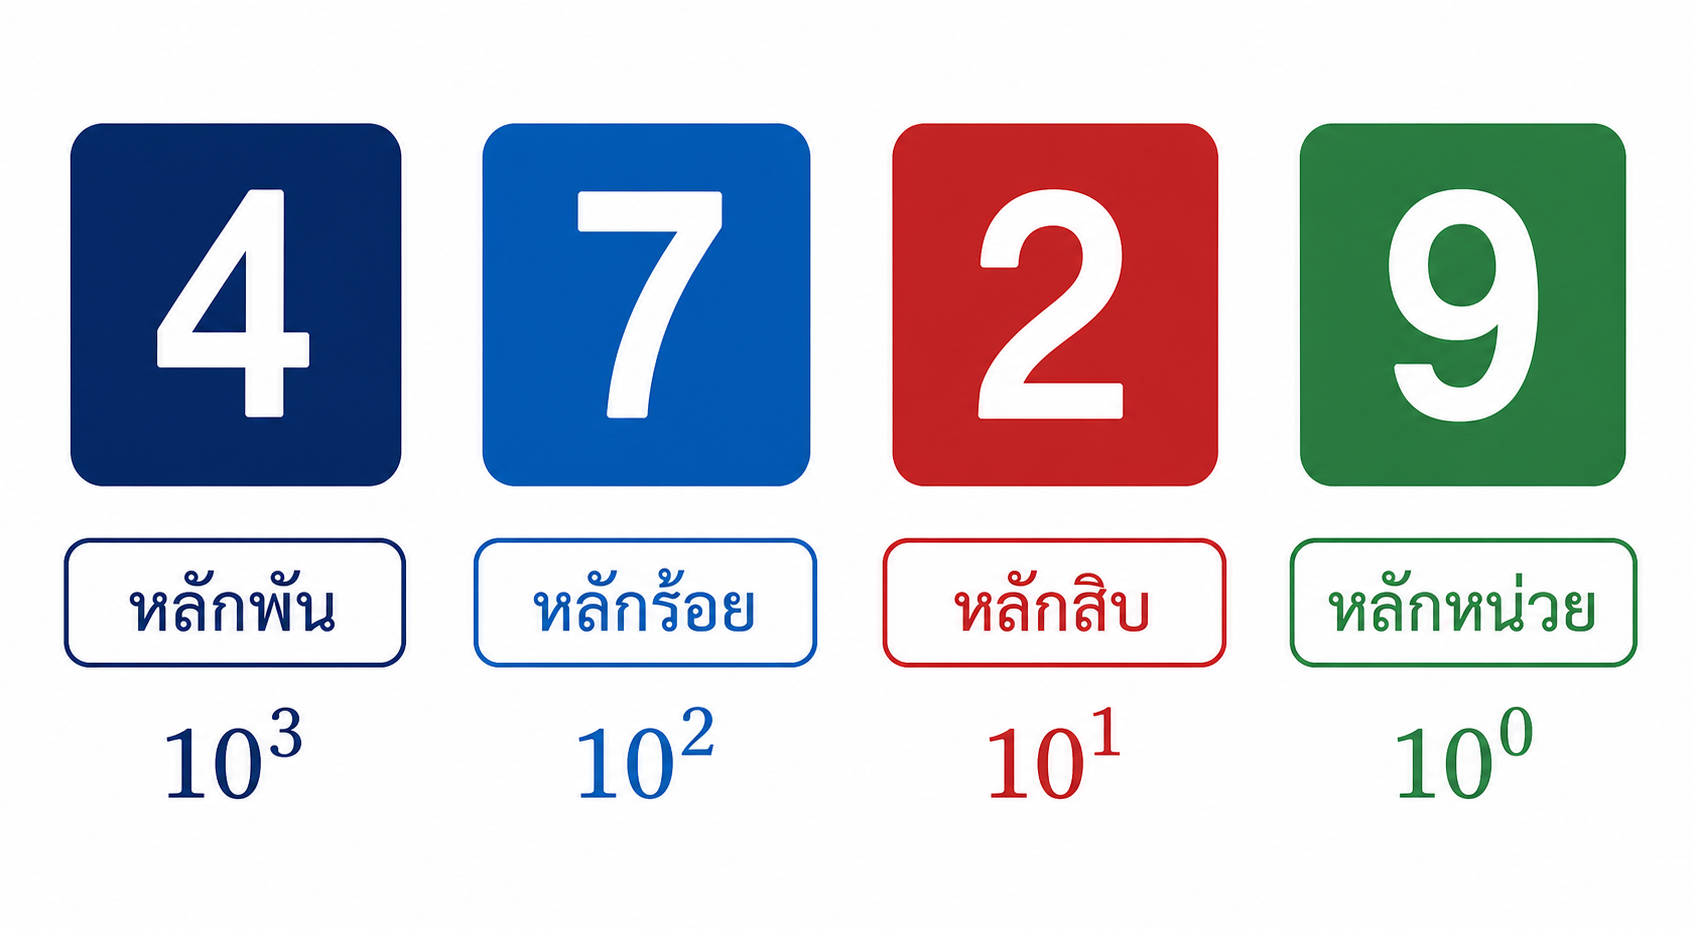
\includegraphics[width=0.62\textwidth]{Figures/png_ready/25-decimal-place-value-manual.png}
    \caption{แผนภาพแสดงค่าประจำหลักของเลขฐานสิบ}
    \label{fig:decimal-place-value}
\end{figure}

ระบบเลขฐานสิบใช้ตัวเลข 10 ตัว และมีฐานเท่ากับ 10 ระบบนี้เป็นระบบที่มนุษย์ใช้มาตลอดประวัติศาสตร์เนื่องจากความสะดวกในการนับด้วยนิ้วมือทั้งสิบนิ้ว การเข้าใจระบบฐานสิบจึงเป็นพื้นฐานสำหรับการศึกษาระบบฐานอื่น

\subsection{ค่าประจำตำแหน่ง}
ในระบบเลขฐานสิบ ค่าของตัวเลขในแต่ละตำแหน่งจะถูกกำหนดโดยผลคูณของตัวเลขหลักนั้นกับ $10^n$ โดย $n$ คือตำแหน่งจากขวาสุดเริ่มนับจากตำแหน่ง 0 สำหรับส่วนจำนวนเต็ม และเริ่มจาก $-1$ ลดลงไปเรื่อยๆ สำหรับส่วนทศนิยม การเข้าใจค่าน้ำหนักประจำหลักนี้เป็นหัวใจสำคัญในการแปลงและทำความเข้าใจระบบเลขฐานอื่นๆ ที่ใช้หลักการเดียวกัน

\begin{thrm}[ค่าประจำตำแหน่งของระบบเลขฐานสิบ]
จำนวนใดๆ ในระบบเลขฐานสิบสามารถเขียนในรูปผลบวกของค่าประจำตำแหน่งได้

$$d_n d_{n-1} \ldots d_1 d_0 . d_{-1} d_{-2} \ldots d_{-m} = \sum_{i=-m}^{n} d_i \times 10^i$$
โดยที่ $d_i$ คือเลขโดดในแต่ละตำแหน่ง และ $10^i$ คือค่าประจำตำแหน่ง
\end{thrm}
\label{thrm:decimal-place-value}

\begin{proof}
การพิสูจน์ค่าประจำตำแหน่งในระบบเลขตำแหน่ง (Positional Notation) พิจารณาเป็นลำดับขั้นตอนดังนี้:
\begin{enumerate}[label=\textbf{\arabic*.}]
    \item \textbf{กำหนดค่าตำแหน่ง:} ให้จำนวนคือ $N = d_n d_{n-1} \ldots d_1 d_0.d_{-1} d_{-2} \ldots d_{-m}$ ในฐาน 10 โดยที่ $d_i$ คือเลขโดดในตำแหน่งที่ $i$
    \item \textbf{คูณน้ำหนักประจำหลัก:} ตัวเลข $d_i$ แต่ละหลักจะมีค่าน้ำหนักเท่ากับกำลังของฐาน 10 นั่นคือ $d_i \times 10^i$
    \item \textbf{รวมผลบวกทุกตำแหน่ง:} นำค่าน้ำหนักทุกหลักตั้งแต่นวนเต็มและส่วนทศนิยมมารวมกัน:
    \[
    N = \sum_{i=-m}^{n} d_i \times 10^i = d_n \times 10^n + d_{n-1} \times 10^{n-1} + \cdots + d_0 \times 10^0 + d_{-1} \times 10^{-1} + \cdots + d_{-m} \times 10^{-m}
    \]
\end{enumerate}
ผลรวมที่ได้สอดคล้องตรงตามนิยามการแทนจำนวนในระบบเลขฐานสิบ
\end{proof}

\begin{ex}[การจำแนกค่าประจำหลักในระบบเลขฐานสิบ]
จงแสดงการกระจายค่าประจำหลักของจำนวนเต็ม $4729$ และจำนวนทศนิยม $53.847$ ในระบบเลขฐานสิบ
\end{ex}
\begin{solution}
สำหรับจำนวนเต็ม $4729$ สามารถกระจายตามค่าประจำหลัก $10^i$ ได้ดังนี้:
\begin{align*}
4729 &= (4\times10^3)+(7\times10^2)+(2\times10^1)+(9\times10^0)\\
     &= 4000+700+20+9
\end{align*}

สำหรับจำนวนทศนิยม $53.847$ สามารถกระจายทั้งส่วนจำนวนเต็มและส่วนทศนิยมได้ดังนี้:
\begin{align*}
53.847 &= (5\times10^1)+(3\times10^0)+(8\times10^{-1})+(4\times10^{-2})+(7\times10^{-3})\\
       &= 50+3+0.8+0.04+0.007
\end{align*}
\solhere
\end{solution}
\label{ex:decimal-place-value}

\section{ระบบเลขฐานสอง (Binary System)}
\zlabel{sec:binary-system}
ระบบเลขฐานสองเป็นระบบเลขพื้นฐานในวิทยาการคอมพิวเตอร์ เนื่องจากวงจรอิเล็กทรอนิกส์และหน่วยความจำของเครื่องคอมพิวเตอร์ทำงานด้วยสัญญาณไฟฟ้าสองสถานะ (เปิดและปิด หรือ สภาวะแรงดันสูงและต่ำ) ระบบนี้ใช้เลขโดดเพียง 2 ตัว คือ $0$ และ $1$ โดยมีค่าประจำหลักเป็นกำลังของฐาน 2 ดังแสดงในรูปที่~\ref{fig:binary-place-value}

\begin{figure}[H]
    \centering
    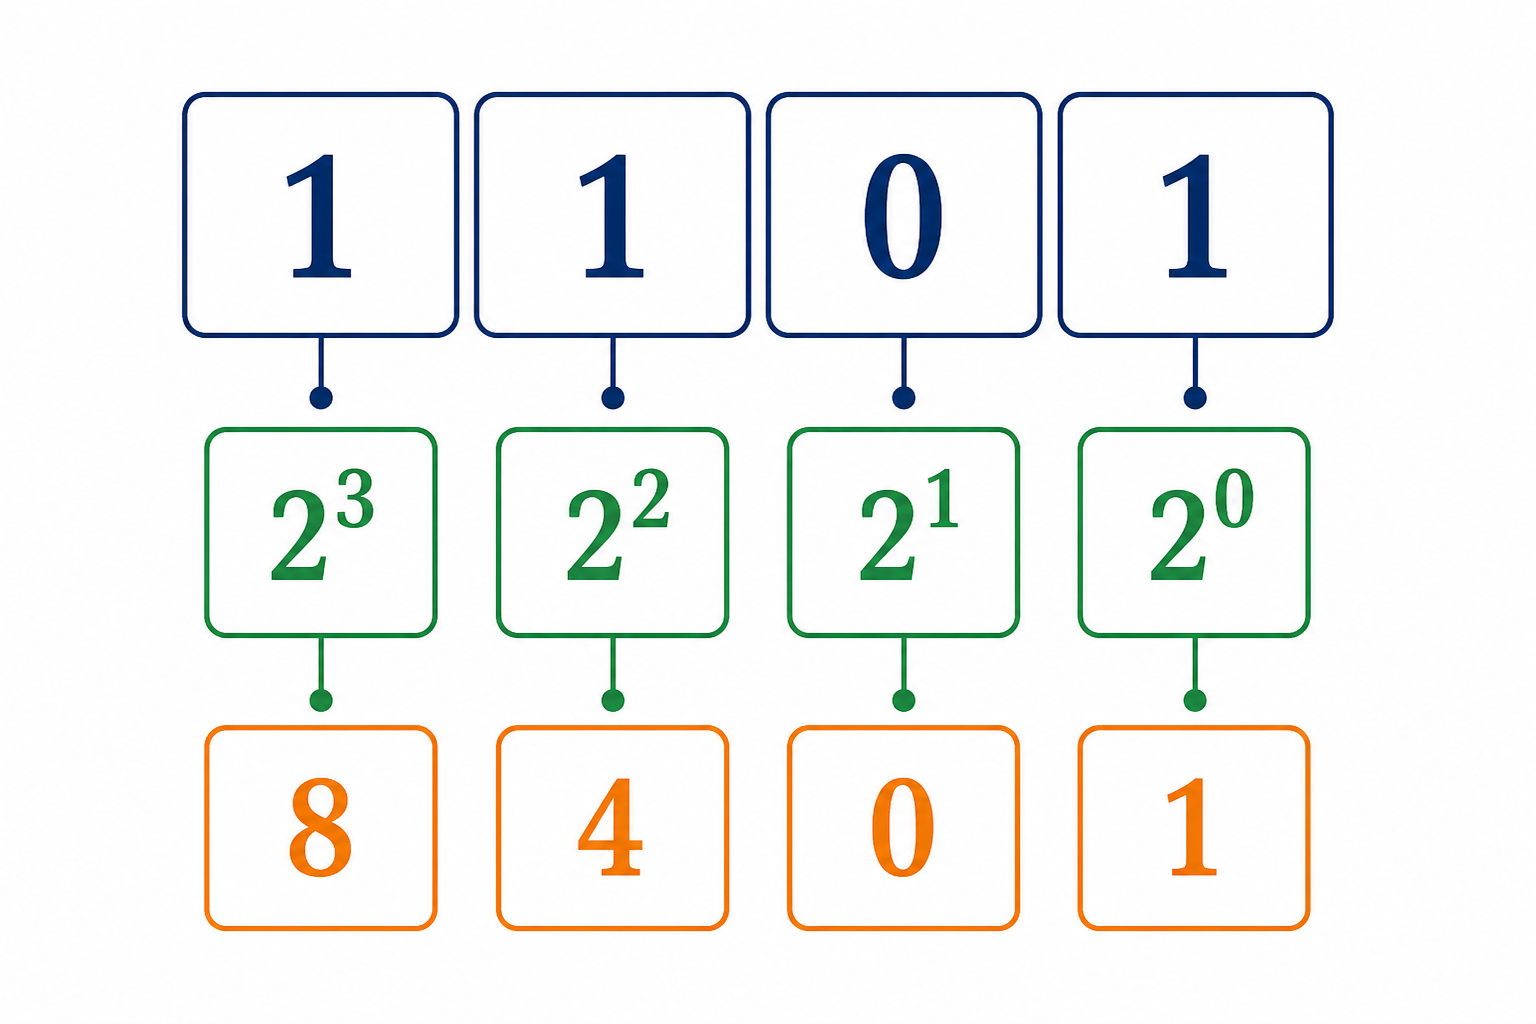
\includegraphics[width=0.62\textwidth]{Figures/png_ready/26-binary-place-value-manual.png}
    \caption{แผนภาพแสดงค่าประจำหลักของเลขฐานสอง}
    \label{fig:binary-place-value}
\end{figure}

รูปที่~\ref{fig:binary-place-value} แสดงบิต $1101$ พร้อมค่าน้ำหนัก $2^3,2^2,2^1,2^0$ ใต้แต่ละตำแหน่ง บิตสามตำแหน่งที่เป็น 1 ให้ค่า $1\times8$, $1\times4$ และ $1\times1$ ส่วนบิตตำแหน่ง $2^1$ เป็น 0 จึงให้ค่าเป็นศูนย์ ดังนั้น $(1101)_2=8+4+0+1=13_{10}$
ระบบเลขฐานสองใช้ตัวเลขเพียง 2 ตัว คือ $0$ และ $1$ และมีฐานเท่ากับ 2 คอมพิวเตอร์ใช้ระบบนี้เพราะวงจรอิเล็กทรอนิกส์สามารถแสดงสองสถานะได้ง่าย (เช่น มีไฟ/ไม่มีไฟ, ปิด/เปิด)
\label{sec:binary-system}

\begin{thrm}
จำนวนในระบบเลขฐานสองสามารถเขียนในรูปผลบวกของ $2^i$ ได้

$$(b_n b_{n-1} \ldots b_1 b_0)_2 = \sum_{i=0}^{n} b_i \times 2^i$$
โดยที่ $b_i \in \{0, 1\}$ แทนเลขโดดแต่ละหลักในฐานสอง
\end{thrm}
\label{thrm:binary-expansion}

\begin{rem}
เลขฐานสอง $(1101)_2$ อ่านว่า ``หนึ่งหนึ่งศูนย์หนึ่งฐานสอง'' ไม่ใช่ ``พันหนึ่งร้อยเอ็ด'' เพราะแต่ละหลักมีค่าประจำตำแหน่งเป็น $2^n$ ไม่ใช่ $10^n$
\end{rem}
\label{rem:binary-reading}

\begin{ex}
แปลง $(1101)_2$ เป็นฐานสิบ
\end{ex}
\begin{solution}
\begin{align*}
(1101)_2 &= (1\times2^3)+(1\times2^2)+(0\times2^1)+(1\times2^0)\\
         &= 8+4+0+1\\
         &= 13
\end{align*}
$\therefore (1101)_2 = (13)_{10}$ \solhere
\end{solution}

\begin{ex}
แปลง $(10110)_2$ เป็นฐานสิบ
\end{ex}
\begin{solution}
\begin{align*}
(10110)_2 &= (1\times2^4)+(0\times2^3)+(1\times2^2)+(1\times2^1)+(0\times2^0)\\
          &= 16+0+4+2+0\\
          &= 22
\end{align*}
$\therefore (10110)_2 = (22)_{10}$ \solhere
\end{solution}

\begin{thrm}
ส่วนทศนิยมในฐานสองมีค่าตามสมการ

$$(0.b_1 b_2 \ldots b_m)_2 = \sum_{i=1}^{m} b_i \times 2^{-i}$$
โดยที่ $b_i \in \{0, 1\}$ แทนเลขโดดในส่วนทศนิยมของฐานสอง
\end{thrm}
\label{thrm:binary-fractional}

\begin{ex}
แปลง $(0.101)_2$ เป็นฐานสิบ
\end{ex}
\begin{solution}
\begin{align*}
(0.101)_2 &= (1\times2^{-1})+(0\times2^{-2})+(1\times2^{-3})\\
          &= \tfrac{1}{2}+0+\tfrac{1}{8}\\
          &= \tfrac{5}{8} = 0.625
\end{align*}
$\therefore (0.101)_2 = (0.625)_{10}$ \solhere
\end{solution}

\begin{ex}
แปลง $(10.011)_2$ เป็นฐานสิบ
\end{ex}
\begin{solution}
\begin{align*}
(10.011)_2 &= (1\times2^1)+(0\times2^0)+(0\times2^{-1})+(1\times2^{-2})+(1\times2^{-3})\\
           &= 2+0+0+0.25+0.125\\
           &= 2.375
\end{align*}
$\therefore (10.011)_2 = (2.375)_{10}$ \solhere
\end{solution}

\section{ระบบเลขฐานแปด (Octal System)}
\zlabel{sec:octal-system}
ระบบเลขฐานแปดใช้ตัวเลข 8 ตัว คือ $0, 1, 2, 3, 4, 5, 6, 7$ และมีฐานเท่ากับ 8 ระบบนี้เคยใช้กันแพร่หลายในยุคแรกของคอมพิวเตอร์เนื่องจากการแปลงระหว่างฐานสองและฐานแปดทำได้ง่าย ทุกตัวเลขฐานแปดสามารถแทนด้วยตัวเลขฐานสอง 3 ตัวพอดี เนื่องจาก $2^3 = 8$ ความสัมพันธ์นี้ทำให้ฐานแปดเป็นวิธีที่สะดวกในการแสดงข้อมูลฐานสองให้อ่านง่ายขึ้น
\label{sec:octal-system}

\begin{thrm}
ความสัมพันธ์ระหว่างฐานสองและฐานแปด: กลุ่มตัวเลขฐานสอง 3 ตัว สามารถแทนด้วยตัวเลขฐานแปด 1 ตัว เนื่องจาก $2^3 = 8$
\end{thrm}
\label{thrm:binary-octal-relation}

\begin{ex}
แปลง $(110101)_2$ เป็นฐานแปด
\end{ex}
\begin{solution}
\begin{align*}
(110101)_2 &= \underbrace{110}_{6}\ \underbrace{101}_{5}\\
           &= (65)_8
\end{align*}
$\therefore (110101)_2 = (65)_8$ \solhere
\end{solution}

\begin{ex}
แปลง $(472)_8$ เป็นฐานสิบ
\end{ex}
\begin{solution}
\begin{align*}
(472)_8 &= (4\times8^2)+(7\times8^1)+(2\times8^0)\\
        &= 256+56+2\\
        &= 314
\end{align*}
$\therefore (472)_8 = (314)_{10}$ \solhere
\end{solution}

\begin{rem}
ฐานแปดเคยใช้กันแพร่หลายในยุคแรกของคอมพิวเตอร์เนื่องจากการแปลงระหว่างฐานสองและฐานแปดทำได้ง่าย ปัจจุบันฐานสิบหกมีการใช้มากกว่า
\end{rem}
\label{rem:octal-history}

\section{ระบบเลขฐานสิบหก (Hexadecimal System)}
\zlabel{sec:hexadecimal-system}
ระบบเลขฐานสิบหกเป็นระบบเลขตำแหน่งที่มีฐานเท่ากับ 16 ใช้สัญลักษณ์ 16 ตัว ประกอบด้วยเลขโดด $0$ ถึง $9$ และตัวอักษรภาษาอังกฤษ $A$ ถึง $F$ (โดย $A=10, B=11, C=12, D=13, E=14, F=15$) ระบบนี้เป็นมาตรฐานในทางคอมพิวเตอร์ เนื่องจากเลขฐานสิบหก 1 หลัก สามารถแทนเลขฐานสองได้ 4 บิตพอดี ช่วยให้ผู้เขียนโปรแกรมอ่านและบันทึกรหัสข้อมูลในหน่วยความจำได้อย่างสะดวก ดังแสดงการจัดกลุ่มในรูปที่~\ref{fig:hex-grouping}

\begin{figure}[H]
    \centering
    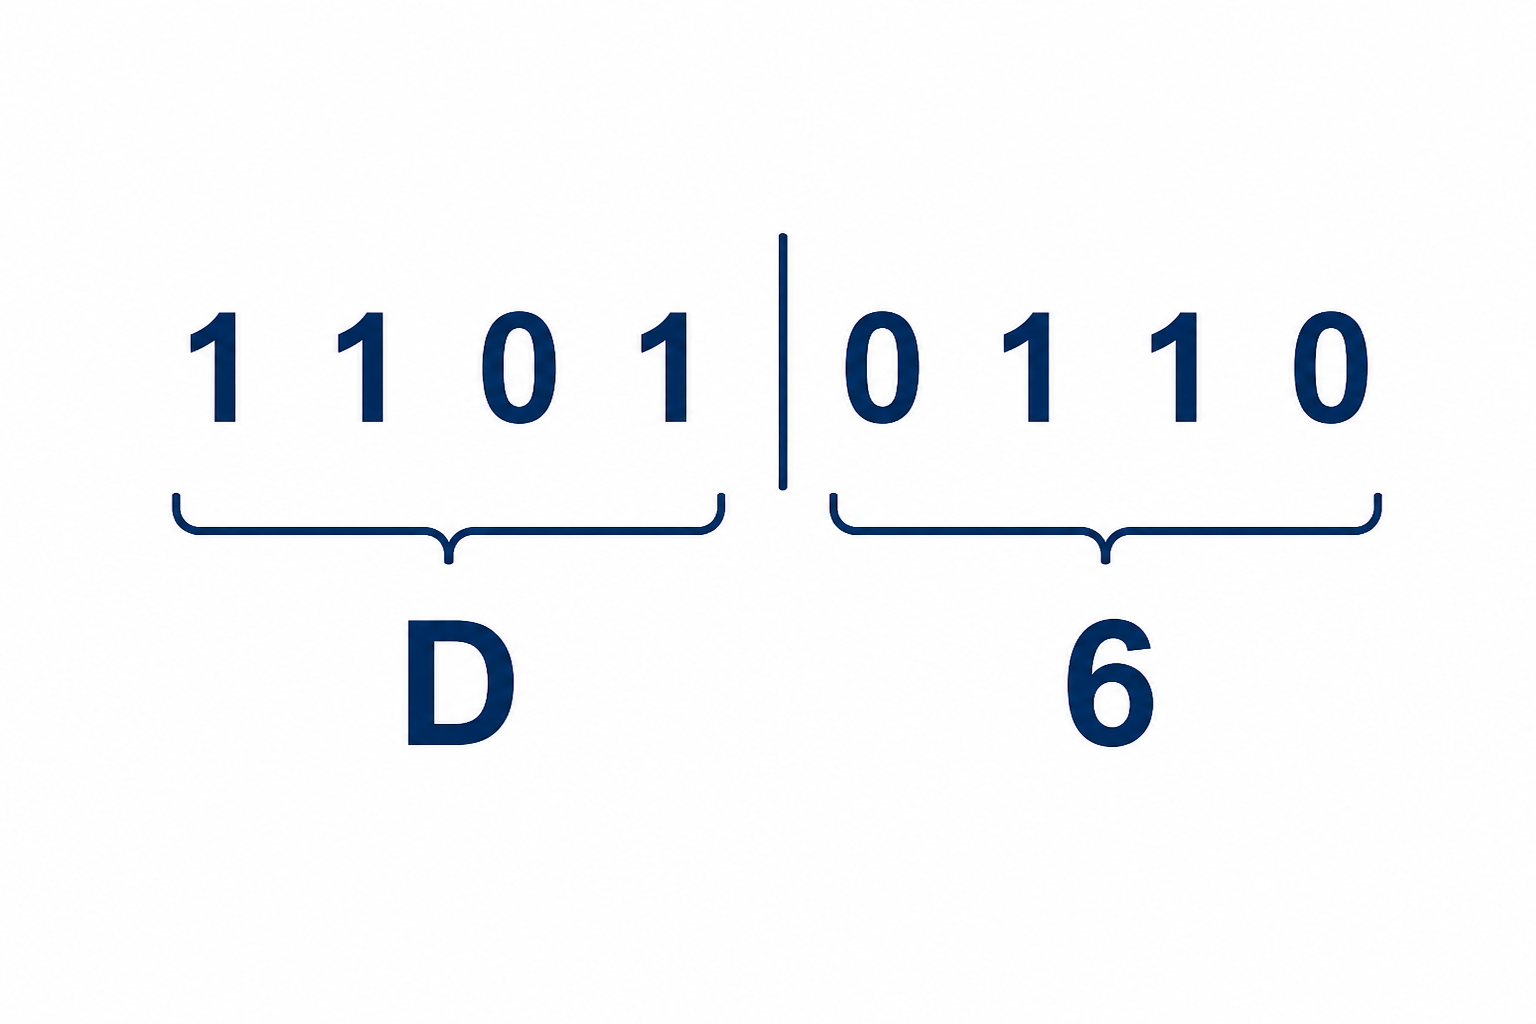
\includegraphics[width=0.62\textwidth]{Figures/png_ready/27-hex-grouping-manual.png}
    \caption{แผนภาพแสดงการจัดกลุ่มเลขฐานสองเป็นเลขฐานสิบหก}
    \label{fig:hex-grouping}
\end{figure}

ระบบเลขฐานสิบหกใช้ตัวเลขและตัวอักษร 16 ตัว คือ $0, 1, 2, 3, 4, 5, 6, 7, 8, 9, A, B, C, D, E, F$ ระบบนี้เป็นมาตรฐานในวงการคอมพิวเตอร์สมัยใหม่เนื่องจากแต่ละตัวอักษรฐานสิบหกแทนได้ด้วยตัวเลขฐานสอง 4 ตัวพอดี เช่นเดียวกับความสัมพันธ์ระหว่างฐานแปดและฐานสอง แต่มีความหนาแน่นของข้อมูลมากกว่าเพราะใช้ทุกตัวในกลุ่ม 4 bits
\label{sec:hexadecimal-system}

\begin{thrm}
ความสัมพันธ์ระหว่างฐานสองและฐานสิบหก: กลุ่มตัวเลขฐานสอง 4 ตัว สามารถแทนด้วยตัวเลขฐานสิบหก 1 ตัว เนื่องจาก $2^4 = 16$
โดยที่แต่ละกลุ่ม 4 bits มีค่าตั้งแต่ $0000_2 = 0$ ถึง $1111_2 = 15 = F_{16}$
\end{thrm}
\label{thrm:binary-hex-relation}

\begin{table}[H]
\centering
\caption{ตารางเปรียบเทียบฐานสิบ ฐานสอง และฐานสิบหก}
\label{tab:binary-hex}
\begin{tabular}{|c|c|c|}
\hline
ฐานสิบ & ฐานสอง (4 หลัก) & ฐานสิบหก \\
\hline
0 & 0000 & 0 \\
1 & 0001 & 1 \\
2 & 0010 & 2 \\
3 & 0011 & 3 \\
4 & 0100 & 4 \\
5 & 0101 & 5 \\
6 & 0110 & 6 \\
7 & 0111 & 7 \\
8 & 1000 & 8 \\
9 & 1001 & 9 \\
10 & 1010 & A \\
11 & 1011 & B \\
12 & 1100 & C \\
13 & 1101 & D \\
14 & 1110 & E \\
15 & 1111 & F \\
\hline
\end{tabular}
\end{table}

\begin{ex}
แปลง $(11010110)_2$ เป็นฐานสิบหก
\end{ex}
\begin{solution}
\begin{align*}
(11010110)_2 &= \underbrace{1101}_{\mathrm{D}}\ \underbrace{0110}_{6}\\
             &= (\mathrm{D}6)_{16}
\end{align*}
$\therefore (11010110)_2 = (\mathrm{D}6)_{16}$ \solhere
\end{solution}

\begin{ex}
แปลง $(3A.F)_{16}$ เป็นฐานสิบ
\end{ex}
\begin{solution}
\begin{align*}
(3A.F)_{16} &= (3\times16^1)+(10\times16^0)+(15\times16^{-1})\\
            &= 48+10+0.9375\\
            &= 58.9375
\end{align*}
$\therefore (3A.F)_{16} = (58.9375)_{10}$ \solhere
\end{solution}

\section{การแปลงฐานทั่วไป}
\zlabel{sec:general-base-conversion}
การแปลงฐานเป็นกระบวนการพื้นฐานที่ใช้ในการสื่อสารระหว่างระบบเลขที่แตกต่างกัน ในทางทฤษฎี การแปลงระหว่างฐานใดๆ สามารถทำได้โดยใช้หลักการของ positional notation ที่สม่ำเสมอ ขั้นตอนการแปลงจะแตกต่างกันขึ้นอยู่กับทิศทางของการแปลงและชนิดของส่วนที่ต้องการแปลง (จำนวนเต็มหรือทศนิยม) การเข้าใจหลักการเบื้องหลังจึงสำคัญกว่าการจำขั้นตอนเพราะทำให้สามารถประยุกต์ใช้กับฐานใดก็ได้
\label{sec:general-base-conversion}

\subsection{การแปลงจากฐานใดๆ เป็นฐานสิบ}
\label{ssec:any-base-to-decimal}
วิธีที่ง่ายที่สุดในการแปลงจากฐานใดๆ เป็นฐานสิบคือการกระจายตามค่าประจำตำแหน่ง

\begin{thrm}
ถ้า $(d_n d_{n-1} \ldots d_1 d_0)_b$ เป็นจำนวนในฐาน $b$ จะมีค่าเท่ากับ

$$(d_n d_{n-1} \ldots d_1 d_0)_b = \sum_{i=0}^{n} d_i \times b^i$$
โดยที่ $d_i$ คือเลขโดดในแต่ละตำแหน่ง และ $b$ คือฐานของระบบเลข
\end{thrm}
\label{thrm:general-base-expansion}

\begin{ex}
แปลง $(2B3)_{16}$ เป็นฐานสิบ และ $(57)_8$ เป็นฐานสิบ
\end{ex}
\begin{solution}
\begin{align*}
(2B3)_{16} &= (2\times16^2)+(11\times16^1)+(3\times16^0)\\
           &= 512+176+3 = 691\\[6pt]
(57)_8     &= (5\times8^1)+(7\times8^0)\\
           &= 40+7 = 47
\end{align*}
$\therefore (2B3)_{16} = (691)_{10}$ และ $(57)_8 = (47)_{10}$ \solhere
\end{solution}

\subsection{การแปลงจากฐานสิบเป็นฐานใดๆ}
\label{ssec:decimal-to-any-base}
ใช้วิธีหารต่อเนื่อง (successive division) โดยหารจำนวนด้วยฐานที่ต้องการแล้วบันทึกเศษ

\begin{thrm}
ขั้นตอนการแปลงจำนวนเต็มจากฐานสิบเป็นฐาน $b$:
\begin{enumerate}
    \item หารจำนวนด้วย $b$ จดเศษไว้
    \item นำผลหารไปหารด้วย $b$ อีก จดเศษ
    \item ทำซ้ำจนกว่าผลหารเป็น 0
    \item เศษที่ได้อ่านจากล่างขึ้นบนคือคำตอบ
\end{enumerate}
\end{thrm}
\label{thrm:decimal-to-any-base-steps}

\begin{ex}
แปลง $45$ ฐานสิบเป็นฐานสอง
\end{ex}
\begin{solution}
\begin{align*}
45 \div 2 &= 22 \quad \text{เศษ } 1\\
22 \div 2 &= 11 \quad \text{เศษ } 0\\
11 \div 2 &= 5  \quad \text{เศษ } 1\\
 5 \div 2 &= 2  \quad \text{เศษ } 1\\
 2 \div 2 &= 1  \quad \text{เศษ } 0\\
 1 \div 2 &= 0  \quad \text{เศษ } 1
\end{align*}
อ่านเศษจากล่างขึ้นบน $\therefore (45)_{10} = (101101)_2$

ตรวจสอบ: $(101101)_2 = 32+8+4+1 = 45$ \checkmark \solhere
\end{solution}

\begin{ex}
แปลง $158$ ฐานสิบเป็นฐานแปด
\end{ex}
\begin{solution}
\begin{align*}
158 \div 8 &= 19 \quad \text{เศษ } 6\\
 19 \div 8 &= 2  \quad \text{เศษ } 3\\
  2 \div 8 &= 0  \quad \text{เศษ } 2
\end{align*}
อ่านเศษจากล่างขึ้นบน $\therefore (158)_{10} = (236)_8$

ตรวจสอบ: $(236)_8 = 128+24+6 = 158$ \checkmark \solhere
\end{solution}

\begin{ex}
แปลง $2543$ ฐานสิบเป็นฐานสิบหก
\end{ex}
\begin{solution}
\begin{align*}
2543 \div 16 &= 158 \quad \text{เศษ } 15\ (\mathrm{F})\\
 158 \div 16 &= 9   \quad \text{เศษ } 14\ (\mathrm{E})\\
   9 \div 16 &= 0   \quad \text{เศษ } 9
\end{align*}
อ่านเศษจากล่างขึ้นบน $\therefore (2543)_{10} = (9\mathrm{EF})_{16}$

ตรวจสอบ: $(9\mathrm{EF})_{16} = 2304+224+15 = 2543$ \checkmark \solhere
\end{solution}

\section{การแปลงจำนวนทศนิยมระหว่างฐาน}
\zlabel{sec:fractional-base-conversion}
การแปลงจำนวนทศนิยมระหว่างฐานมีความซับซ้อนมากกว่าจำนวนเต็มเนื่องจากการคูณต่อเนื่องอาจให้ผลลัพธ์เป็นทศนิยมซ้ำไม่รู้จบในบางฐาน โดยเฉพาะการแปลงทศนิยมฐานสิบเป็นฐานสองนั้น จำนวนที่ดูเหมือนง่ายอย่าง $0.1_{10}$ กลับมีค่าเป็นทศนิยมซ้ำไม่รู้จบในฐานสอง ปรากฏการณ์นี้เป็นที่มาของปัญหา floating-point error ที่พบได้บ่อยในการคำนวณด้วยคอมพิวเตอร์
\label{sec:fractional-base-conversion}

\subsection{การแปลงส่วนทศนิยมจากฐานสิบเป็นฐานอื่น}
\label{ssec:fractional-conversion}
ใช้วิธีคูณต่อเนื่อง (successive multiplication) กับส่วนทศนิยม

\begin{thrm}
ขั้นตอนการแปลงส่วนทศนิยมจากฐานสิบเป็นฐาน $b$:
\begin{enumerate}
    \item คูณส่วนทศนิยมด้วย $b$
    \item บันทึกผลคูณที่เป็นจำนวนเต็ม (0 หรือ 1 สำหรับฐานสอง) เป็นเลขหลักถัดไป
    \item นำส่วนทศนิยมของผลคูณไปคูณต่อ
    \item ทำซ้ำจนกว่าส่วนทศนิยมเป็น 0 หรือได้จำนวนหลักตามต้องการ
\end{enumerate}
\end{thrm}
\label{thrm:fractional-conversion-steps}

\begin{ex}
แปลง $0.625$ ฐานสิบเป็นฐานสอง
\end{ex}
\begin{solution}
\begin{align*}
0.625 \times 2 &= 1.25 \quad \text{หลัก } 1\\
0.25  \times 2 &= 0.5  \quad \text{หลัก } 0\\
0.5   \times 2 &= 1.0  \quad \text{หลัก } 1
\end{align*}
อ่านหลักจากบนลงล่าง $\therefore (0.625)_{10} = (0.101)_2$

ตรวจสอบ: $(0.101)_2 = 0.5+0.125 = 0.625$ \checkmark \solhere
\end{solution}

\begin{ex}
แปลง $0.7$ ฐานสิบเป็นฐานสอง (แสดง 8 หลัก)
\end{ex}
\begin{solution}
\begin{align*}
0.7 \times 2 &= 1.4 \quad \text{หลัก } 1\\
0.4 \times 2 &= 0.8 \quad \text{หลัก } 0\\
0.8 \times 2 &= 1.6 \quad \text{หลัก } 1\\
0.6 \times 2 &= 1.2 \quad \text{หลัก } 1\\
0.2 \times 2 &= 0.4 \quad \text{หลัก } 0\\
0.4 \times 2 &= 0.8 \quad \text{หลัก } 0\\
0.8 \times 2 &= 1.6 \quad \text{หลัก } 1\\
0.6 \times 2 &= 1.2 \quad \text{หลัก } 1
\end{align*}
ส่วนทศนิยม $0.4$ วนซ้ำ ทำให้ได้ทศนิยมซ้ำไม่รู้จบ เมื่อแสดง 8 หลักได้ $(0.7)_{10} \approx (0.10110011)_2$ และค่าที่แท้จริงคือ $(0.7)_{10} = (0.1\overline{0110})_2$ \solhere
\end{solution}

\begin{ex}
แปลง $0.3125$ ฐานสิบเป็นฐานแปด
\end{ex}
\begin{solution}
\begin{align*}
0.3125 \times 8 &= 2.5 \quad \text{หลัก } 2\\
0.5    \times 8 &= 4.0 \quad \text{หลัก } 4
\end{align*}
อ่านหลักจากบนลงล่าง $\therefore (0.3125)_{10} = (0.24)_8$

ตรวจสอบ: $(0.24)_8 = \tfrac{2}{8}+\tfrac{4}{64} = 0.25+0.0625 = 0.3125$ \checkmark \solhere
\end{solution}

\section{การบวกและลบเลขฐานสอง}
\zlabel{sec:binary-add-sub}
การบวกและลบเลขฐานสองเป็นการดำเนินการพื้นฐานที่วงจรคอมพิวเตอร์ใช้ในการคำนวณทุกระดับ หลักการเหมือนกับการบวกลบฐานสิบแต่ใช้ฐาน 2 แทน การเข้าใจการทำงานของ carry และ borrow ในฐานสองจึงเป็นพื้นฐานสำคัญสำหรับการออกแบบ ALU (Arithmetic Logic Unit)
\label{sec:binary-add-sub}

\subsection{การบวกเลขฐานสอง}
การบวกเลขฐานสองมีกฎพื้นฐานดังนี้
\begin{thrm}
การบวกเลขฐานสอง

\begin{enumerate}
    \item $0 + 0 = 0$
    \item $0 + 1 = 1$
    \item $1 + 0 = 1$
    \item $1 + 1 = 10$ (เป็น 0 ทด 1)
    \item $1 + 1 + 1 = 11$ (เป็น 1 ทด 1)
\end{enumerate}
\end{thrm}
\label{thrm:binary-addition-rules}

\begin{ex}
บวก $(1011)_2$ กับ $(1101)_2$:
\end{ex}

\begin{solution}
\[
\begin{array}{r}
1011 \\
+\,1101 \\
\hline
11000
\end{array}
\]
$\therefore (1011)_2 + (1101)_2 = (11000)_2$

ตรวจสอบ: $(1011)_2 = 11_{10}$, $(1101)_2 = 13_{10}$, และ $11+13 = 24 = (11000)_2$ \checkmark \solhere
\end{solution}

\begin{ex}
บวก $(1111)_2$ กับ $(0001)_2$:
\end{ex}

\begin{solution}
\[
\begin{array}{r}
1111 \\
+\,0001 \\
\hline
10000
\end{array}
\]
$\therefore (1111)_2 + (0001)_2 = (10000)_2 = (16)_{10}$ \solhere
\end{solution}

\subsection{การลบเลขฐานสอง}
\label{ssec:binary-subtraction}
การลบเลขฐานสองใช้หลักการขอยืม (Borrowing) ในลักษณะเดียวกับการลบเลขฐานสิบในชีวิตประจำวัน โดยเมื่อตัวตั้งมีค่าน้อยกว่าตัวลบในหลักเดียวกัน จะต้องทำการขอยืมค่าน้ำหนักจากหลักที่อยู่ทางซ้ายมือซึ่งมีค่าเป็น 2 เท่าของหลักปัจจุบัน ในระบบคอมพิวเตอร์ การลบสามารถทำได้ทั้งการลบโดยตรงและการแปลงให้อยู่ในรูปการบวกด้วยส่วนเติมเต็ม (Complement)

\begin{thrm}
การลบเลขฐานสอง

\begin{enumerate}
    \item $0 - 0 = 0$
    \item $1 - 0 = 1$
    \item $1 - 1 = 0$
    \item $0 - 1 = 1$ (ยืม 1 จากหลักซ้าย ทำให้หลักซ้ายลดลง 1)
\end{enumerate}
\end{thrm}
\label{thrm:binary-subtraction-rules}

\begin{ex}
ลบ $(1100)_2$ ด้วย $(0101)_2$:
\end{ex}

\begin{solution}
\[
\begin{array}{r}
1100 \\
-\,0101 \\
\hline
0111
\end{array}
\]
$\therefore (1100)_2 - (0101)_2 = (0111)_2$

ตรวจสอบ: $(1100)_2 = 12_{10}$, $(0101)_2 = 5_{10}$, และ $12-5 = 7 = (0111)_2$ \checkmark \solhere
\end{solution}

\begin{ex}
ลบ $(1000)_2$ ด้วย $(0001)_2$ (แสดงขั้นตอนการยืม)

\end{ex}

\begin{solution}
\[
\begin{array}{r}
1000 \\
-\,0001 \\
\hline
0111
\end{array}
\]
การยืมต่อเนื่อง: หลักขวาสุด $0-1$ ต้องยืมจากหลักที่สี่ผ่านหลักที่สองและสาม ทำให้ $1000_2$ กลายเป็นค่าประจำหลัก $0,1,1,10_2$ ก่อนลบ

$\therefore (1000)_2 - (0001)_2 = (0111)_2$

ตรวจสอบ: $(1000)_2 = 8_{10}$, $(0001)_2 = 1_{10}$, และ $8-1 = 7 = (0111)_2$ \checkmark \solhere
\end{solution}

\section{การคูณและการหารเลขฐานสอง}
\zlabel{sec:binary-mult-div}
การคูณเลขฐานสองมีข้อได้เปรียบที่สำคัญคือผลคูณของแต่ละหลักมีได้เพียง 0 หรือ 1 ทำให้การคูณลดรูปเป็นการ shift และบวก ซึ่งเป็นการดำเนินการที่วงจรดิจิทัลทำได้อย่างมีประสิทธิภาพ หลักการนี้เป็นพื้นฐานของ multiplier ในหน่วยประมวลผลกลาง
\label{sec:binary-mult-div}

\subsection{การคูณเลขฐานสอง}
การคูณเลขฐานสองมีโครงสร้างที่ง่ายและเป็นระเบียบเนื่องจากตัวคูณในแต่ละตำแหน่งมีเพียงสัญลักษณ์ 0 หรือ 1 เท่านั้น เมื่อตัวคูณเป็น 0 ผลคูณย่อยจะเป็น 0 ทั้งหมด และเมื่อตัวคูณเป็น 1 ผลคูณย่อยจะเท่ากับตัวตั้งเดิม กระบวนการคูณในคอมพิวเตอร์จึงลดรูปเหลือเพียงการเลื่อนตำแหน่งบิต (Bit Shift) และการบวกสะสมผลลัพธ์ย่อยเข้าด้วยกัน

\begin{thrm}
การคูณเลขฐานสอง

\begin{enumerate}
    \item $0 \times 0 = 0$
    \item $0 \times 1 = 0$
    \item $1 \times 0 = 0$
    \item $1 \times 1 = 1$
\end{enumerate}
\end{thrm}
\label{thrm:binary-multiplication-rules}

\begin{ex}
คูณ $(1011)_2$ ด้วย $(1101)_2$:
\end{ex}

\begin{solution}
\[
\begin{array}{r}
1011 \\
\times\,1101 \\
\hline
1011 \\
0000\phantom{0} \\
1011\phantom{00} \\
1011\phantom{000} \\
\hline
10001111
\end{array}
\]
$\therefore (1011)_2 \times (1101)_2 = (10001111)_2$

ตรวจสอบ: $(1011)_2 = 11_{10}$, $(1101)_2 = 13_{10}$, และ $11\times13 = 143 = (10001111)_2$ \checkmark \solhere
\end{solution}

\begin{rem}
การคูณเลขฐานสองในคอมพิวเตอร์ใช้วิธี shift-and-add ซึ่งประสิทธิภาพกว่าการคูณแบบธรรมดามาก
\end{rem}
\label{rem:shift-add}

\section{การแทนจำนวนเต็มลบในฐานสอง}
\zlabel{sec:negative-binary}
ในคอมพิวเตอร์ จำนวนเต็มลบต้องมีการแทนที่พิเศษ เนื่องจากไม่มีเครื่องหมายลบในฐานสอง มี 3 วิธีหลักที่ใช้กัน ได้แก่ Signed Magnitude, 1's Complement และ 2's Complement แต่ละวิธีมีข้อดีข้อเสียแตกต่างกัน และมีผลต่อช่วงของจำนวนที่สามารถแทนได้รวมถึงวิธีการบวกลบในระบบ การเข้าใจความแตกต่างของแต่ละวิธีจึงมีความสำคัญต่อการเขียนโปรแกรมระดับต่ำและการออกแบบระบบดิจิทัล
\label{sec:signed-number-representation}

\subsection{Signed Magnitude (Sign-Magnitude)}
\label{ssec:sign-magnitude}
ใช้หลักซ้ายสุดเป็น bit สำหรับเครื่องหมาย (0 = บวก, 1 = ลบ) และหลักที่เหลือเป็นค่าสัมบูรณ์

\begin{thrm}
ในระบบ signed magnitude ขนาด $n$ bits:
\begin{enumerate}
    \item bit ซ้ายสุด = เครื่องหมาย (0 บวก, 1 ลบ)
    \item bits ที่เหลือ = ค่าสัมบูรณ์
    \item ช่วง $-(2^{n-1}-1)$ ถึง $+(2^{n-1}-1)$
    \item มี 0 สองแบบ คือ $+0$ และ $-0$
\end{enumerate}
\end{thrm}
\label{thrm:sign-magnitude}

\begin{ex}
ในระบบ signed magnitude 8 bits: $+45$ และ $-45$ แทนด้วย binary อย่างไร
\end{ex}
\begin{solution}
\begin{align*}
45  &= (0101101)_2 \quad (\text{ส่วนขนาด 7 บิต})\\
+45 &= (\underline{0}\,0101101)_2 = (00101101)_2\\
-45 &= (\underline{1}\,0101101)_2 = (10101101)_2
\end{align*}
โดยบิตซ้ายสุดที่ขีดเส้นใต้คือบิตเครื่องหมาย \solhere
\end{solution}

\begin{rem}
วิธี signed magnitude ไม่ค่อยใช้ในปัจจุบันเพราะมี 0 สองแบบและวงจรลำบาก
\end{rem}
\label{rem:sign-magnitude-rarely-used}

\subsection{1's Complement}
\label{ssec:ones-complement}
การแทนจำนวนลบโดยการกลับ bit ทุก bit ของจำนวนบวก

\begin{thrm}
ในระบบ 1's complement ขนาด $n$ bits:
\begin{enumerate}
    \item ค่าบวก เหมือน unsigned
    \item ค่าลบ คือ กลับ bit ทุก bit ของค่าบวก
    \item ช่วง $-(2^{n-1}-1)$ ถึง $+(2^{n-1}-1)$
    \item ยังมี 0 สองแบบ คือ $+0 = 00000000$, $-0 = 11111111$
\end{enumerate}
\end{thrm}
\label{thrm:ones-complement}

\begin{prop}
ในระบบ 1's complement $n$ bits สำหรับจำนวนเต็ม $x$ ใดๆ ที่ $0 \leq x < 2^{n-1}$ จะได้ว่า $x + \overline{x} = 2^n - 1$ เมื่อ $\overline{x}$ คือ bitwise complement ของ $x$
\end{prop}

\begin{ex}
ในระบบ 1's complement 8 bits:
\end{ex}
\begin{solution}
\begin{align*}
+45 &= (00101101)_2\\
-45 &= (11010010)_2 \quad (\text{กลับบิตทุกบิต})
\end{align*}
การบวกใน 1's complement ต้องมี end-around carry
\[ (00101101)_2 + (11010010)_2 = (11111111)_2 = -0 \]
\end{solution}

\subsection{2's Complement}
\begin{figure}[H]
    \centering
    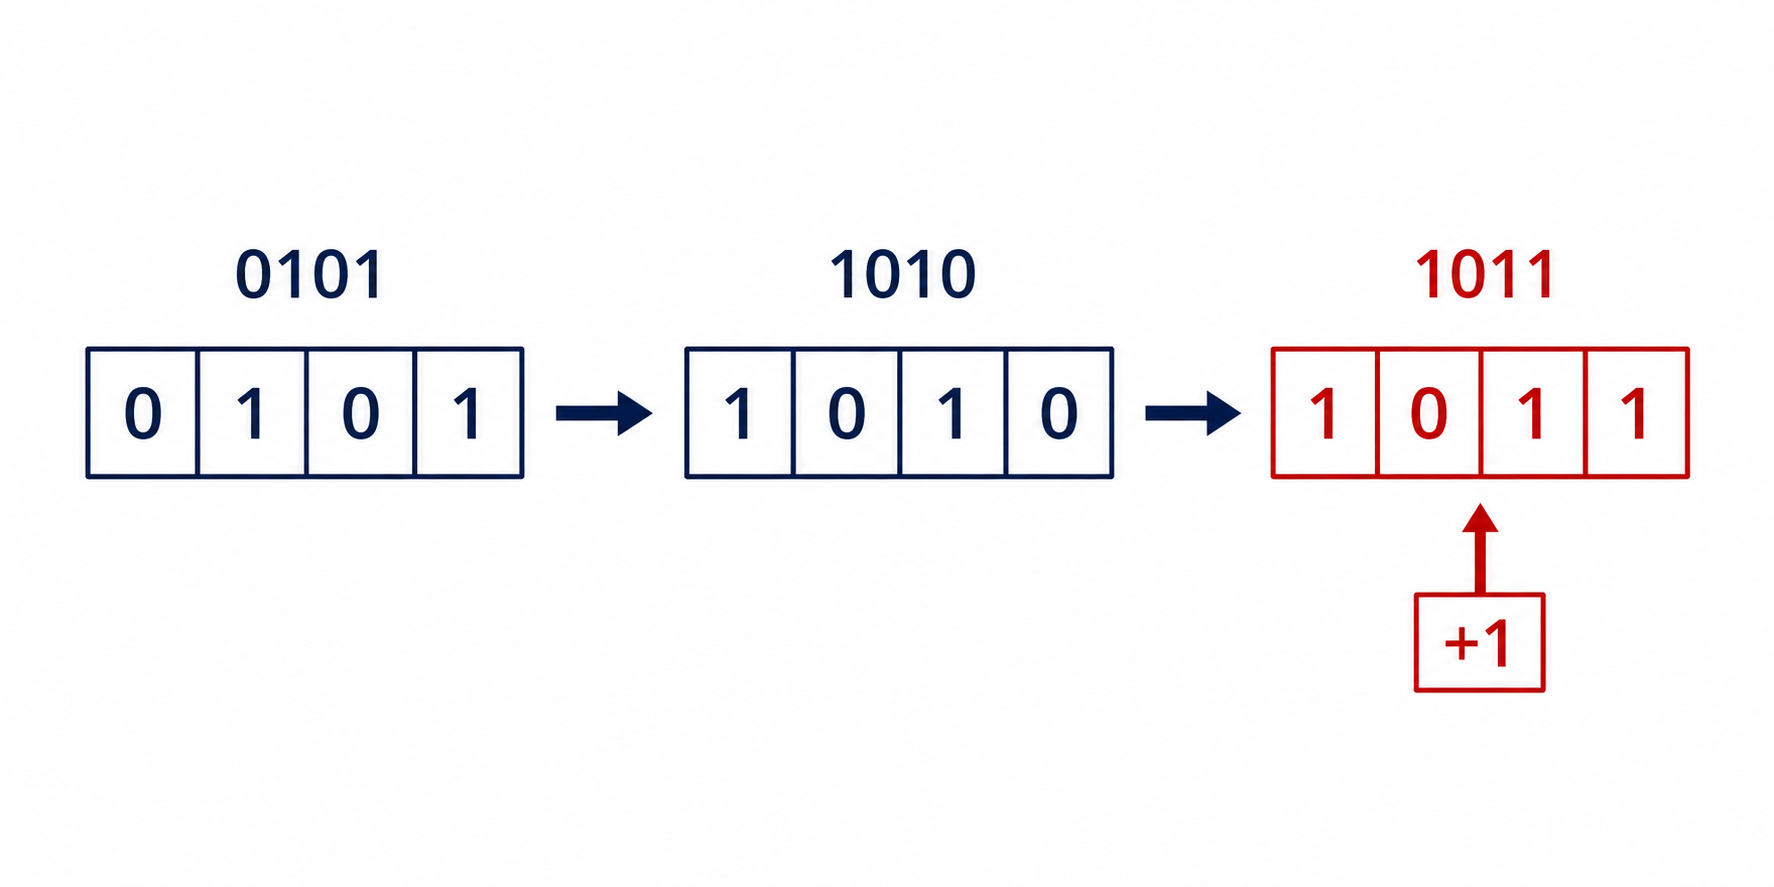
\includegraphics[width=0.62\textwidth]{Figures/png_ready/28-2s-complement-manual.png}
    \caption{แผนภาพแสดงขั้นตอนการสร้างส่วนเติมเต็มสอง}
    \label{fig:2s-complement}
\end{figure}

\label{ssec:twos-complement}
รูปที่~\ref{fig:2s-complement} แสดงลำดับการทำงานจากซ้ายไปขวา เริ่มจาก $0101$ ซึ่งเป็นจำนวนบวก กลับค่าบิตทีละตำแหน่งเป็น $1010$ แล้วบวก $0001$ ตามลูกศร ผลลัพธ์คือ $1011$ ซึ่งใช้แทนค่าลบของจำนวนเดิมในระบบส่วนเติมเต็มสองแบบ 4 บิต
วิธีที่ใช้กันมากที่สุดในคอมพิวเตอร์ปัจจุบัน

\begin{thrm}
ในระบบ 2's complement ขนาด $n$ bits:
\begin{enumerate}
    \item ค่าบวก เหมือน unsigned
    \item ค่าลบ คือ กลับ bit ทุก bit แล้วบวก 1 หรือเทียบเท่ากับ $2^n - |x|$
    \item ช่วง $-2^{n-1}$ ถึง $+(2^{n-1}-1)$
    \item มี 0 แบบเดียว คือ $00000000$
    \item การบวกปกติใช้ได้เลยโดยไม่ต้อง special case
\end{enumerate}
\label{thrm:twos-complement}
\end{thrm}

\begin{prop}
ในระบบ 2's complement $n$ bits สำหรับจำนวนเต็ม $x$ ใดๆ จะได้ว่า $-x \equiv 2^n - x \pmod{2^n}$ และ $-x$ หาได้โดยการกลับ bit ทุก bit แล้วบวก 1
\end{prop}

\begin{ex}[การหาค่า 2's Complement]
จงหาค่า $-45$ ในระบบ 2's complement ขนาด 8 บิต
\end{ex}
\begin{solution}
\begin{align*}
+45 &= (00101101)_2\\
-45 &= (11010011)_2 \quad (\text{กลับบิตแล้วบวก 1})
\end{align*}
ตรวจสอบ: $(00101101)_2 + (11010011)_2 = (1\,00000000)_2 \equiv (00000000)_2$ (ตัดบิตทดซ้ายสุดทิ้ง) \solhere
\end{solution}

\begin{ex}
หาค่าของ $11010011_2$ ในระบบ 2's complement 8 bits:
\end{ex}
\begin{solution}
บิตซ้ายสุดเป็น 1 จึงเป็นจำนวนลบ หาค่าสัมบูรณ์โดยกลับบิตแล้วบวก 1
\begin{align*}
(11010011)_2 \xrightarrow{\text{กลับบิต}} (00101100)_2 \xrightarrow{+1} (00101101)_2 = 45
\end{align*}
$\therefore (11010011)_2 = -45$
\end{solution}

\begin{thrm}
ช่วงค่าในระบบ 2's complement $n$ bits:
\begin{enumerate}
    \item ค่าบวกมากที่สุด คือ $2^{n-1} - 1$ (เช่น 127 ใน 8 bits)
    \item ค่าลบน้อยที่สุด คือ $-2^{n-1}$ (เช่น -128 ใน 8 bits)
    \item ไม่มี $-0$ เพราะ $-128$ ใช้ $10000000_2$
\end{enumerate}
\label{thrm:twos-complement-range}
\end{thrm}

\section{การบวกและลบในฐานสิบหก}
\zlabel{sec:hex-arithmetic}
การบวกและลบในฐานสิบหกมีหลักการเหมือนกับฐานสิบทุกประการ แต่ตัวเลขสูงสุดในแต่ละหลักคือ $F$ (ค่า 15) แทนที่จะเป็น $9$ การบวกจึงต้องทดเมื่อผลลัพธ์เกิน $F$ ซึ่งเทียบเท่ากับการทดเมื่อผลบวกเกิน 9 ในฐานสิบ ความเข้าใจในการดำเนินการฐานสิบหกมีความสำคัญในการเขียนโปรแกรมระดับต่ำ การแก้ไขข้อมูลในหน่วยความจำ และการใช้เครื่องมือ debug

\begin{thrm}
ถ้าผลบวกของแต่ละหลักเกิน $F_{16}$ ให้ทด 1 ไปหลักซ้าย และเขียนผลลัพธ์ลบ 16
โดยที่ $F_{16}$ มีค่าเท่ากับ 15 ในฐานสิบ การทด 1 หลักในฐานสิบหกหมายถึงการบวก $16$ เข้าไปในผลลัพธ์
\end{thrm}
\label{thrm:hex-addition-carry}

\begin{ex}
บวก $(3A5)_{16}$ กับ $(1F7)_{16}$:
\end{ex}

\begin{solution}
\[
\begin{array}{r}
3A5 \\
+\,1F7 \\
\hline
59C
\end{array}
\]
$\therefore (3A5)_{16} + (1F7)_{16} = (59C)_{16}$

ตรวจสอบ: $(3A5)_{16} = 933_{10}$, $(1F7)_{16} = 503_{10}$, และ $933+503 = 1436 = (59C)_{16}$ \checkmark
\end{solution}

\begin{ex}
ลบ $(9F2)_{16}$ ด้วย $(3A4)_{16}$:
\end{ex}

\begin{solution}
\[
\begin{array}{r}
9F2 \\
-\,3A4 \\
\hline
64E
\end{array}
\]
$\therefore (9F2)_{16} - (3A4)_{16} = (64E)_{16}$

ตรวจสอบ: $(9F2)_{16} = 2546_{10}$, $(3A4)_{16} = 932_{10}$, และ $2546-932 = 1614 = (64E)_{16}$ \checkmark
\end{solution}

\section{IEEE 754  การแทนทศนิยมในคอมพิวเตอร์}
\zlabel{sec:ieee754}
มาตรฐาน IEEE 754 (Institute of Electrical and Electronics Engineers) เป็นมาตรฐานสากลที่ใช้ในการจัดเก็บและคำนวณจำนวนจริงในรูปเลขทศนิยมลอยตัว (Floating-Point Numbers) ในหน่วยประมวลผลของคอมพิวเตอร์ทุกชนิด การเข้าใจโครงสร้าง IEEE 754 ช่วยให้โปรแกรมเมอร์เข้าใจเรื่องขอบเขตความแม่นยำและความผิดพลาดจากการปัดเศษ (Floating-point error) โดยแบ่งข้อมูลออกเป็น 3 ส่วนหลัก ได้แก่ บิตเครื่องหมาย เลขชี้กำลัง และแมนทิสซา ดังแสดงในรูปที่~\ref{fig:ieee754}

\begin{figure}[H]
    \centering
    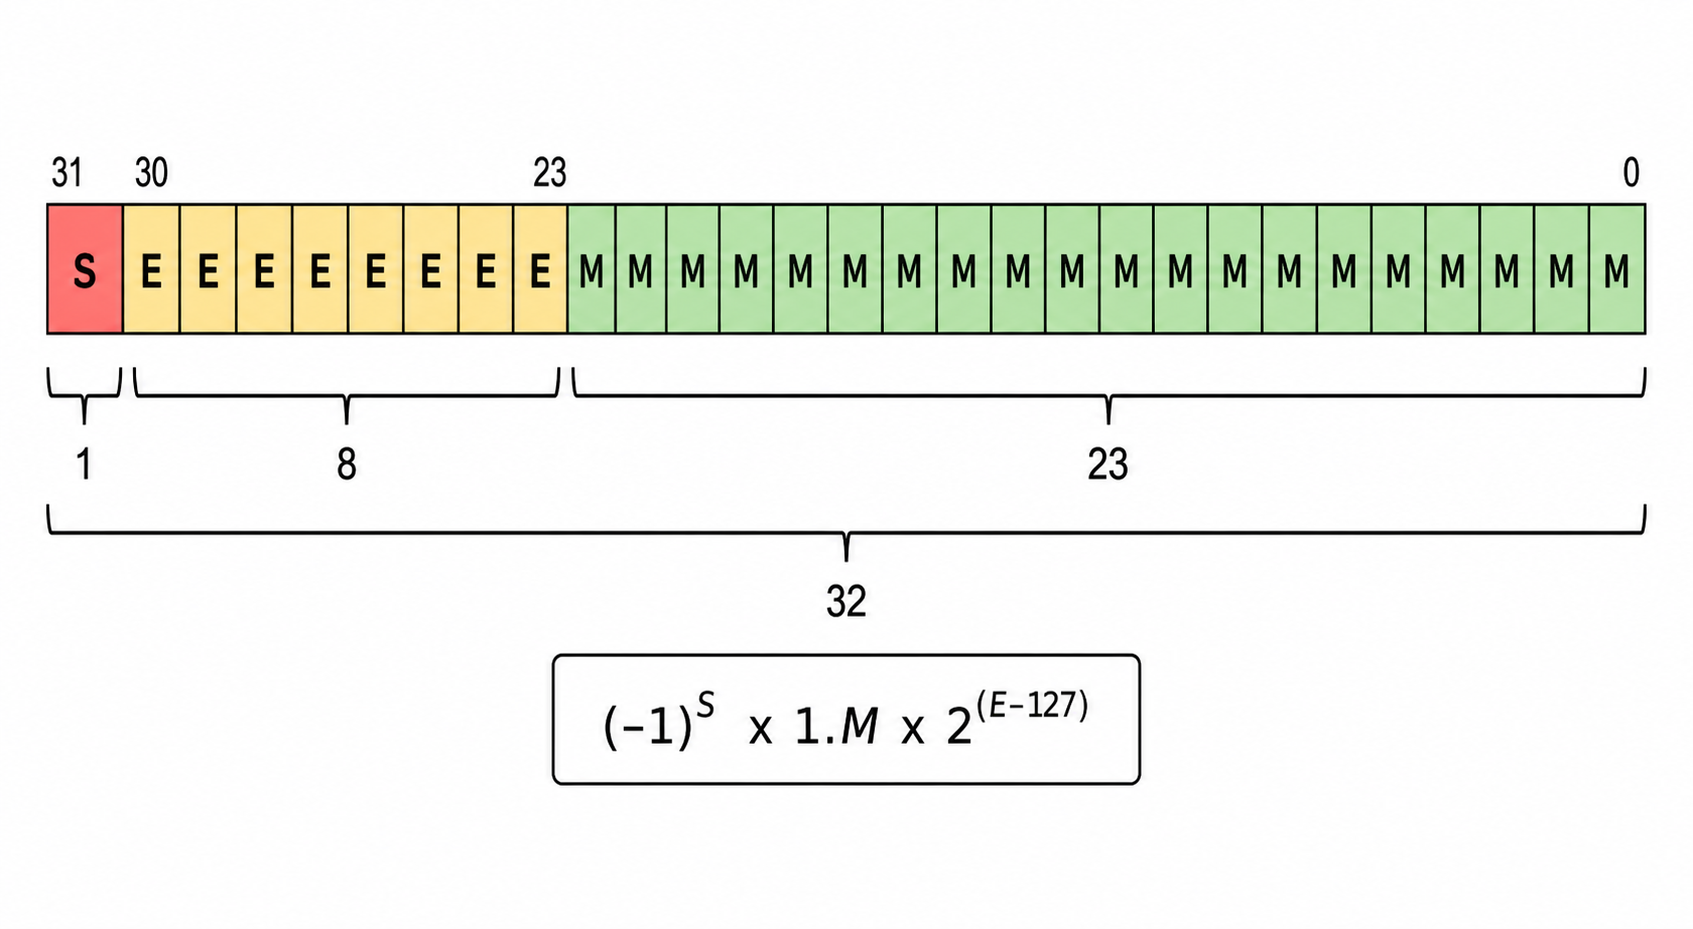
\includegraphics[width=0.62\textwidth]{Figures/png_ready/29-ieee754-manual.png}
    \caption{แผนภาพแสดงโครงสร้างการแทนเลขแบบ IEEE 754 ความละเอียดเดี่ยว}
    \label{fig:ieee754}
\end{figure}

\subsection{โครงสร้างของ IEEE 754 Single Precision (32 bits)}
\label{ssec:ieee-754-single-precision}
มาตรฐาน IEEE 754 กำหนดวิธีเก็บจำนวนจริงในรูปเลขทศนิยมลอยตัว (floating point) โดยแบ่งบิตออกเป็นส่วน ๆ ที่มีหน้าที่ต่างกัน แบบ single precision ใช้ทั้งหมด 32 บิต

\begin{definition}[โครงสร้าง IEEE 754 Single Precision]
\index{IEEE 754!โครงสร้าง}
จำนวน single precision 32 bits แบ่งเป็น 3 ส่วน ดังนี้
\begin{enumerate}
    \item บิตเครื่องหมาย ($S$) ขนาด 1 บิต (0 แทนบวก, 1 แทนลบ)
    \item เลขชี้กำลัง ($E$) ขนาด 8 บิต (ปรับเอียงด้วยไบแอส)
    \item ส่วนเศษ ($F$) ขนาด 23 บิต (แมนทิสซา)
\end{enumerate}
ค่าจริงของจำนวนคือ
\[ (-1)^S \times 1.F \times 2^{E-127} \]
\end{definition}
\label{thrm:ieee-754-structure}

โดยที่ $S$ คือ sign bit กำหนดเครื่องหมายของจำนวน, $E$ คือ biased exponent ซึ่งมี bias เท่ากับ 127 สำหรับ single precision และ $F$ คือ fraction (mantissa) ที่อยู่หลังจุดทศนิยม

\begin{prop}
เหตุผลที่ใช้ bias 127 สำหรับ single precision คือเพื่อให้ค่า exponent ที่เก็บเป็นจำนวนไม่ติดลบตั้งแต่ 0 ถึง 255 ทำให้การเปรียบเทียบทำได้ง่าย สำหรับ normalized numbers ค่า exponent field จะอยู่ในช่วง 1 ถึง 254 จึงทำให้ค่า exponent จริงอยู่ในช่วง $-126$ ถึง $+127$ ส่วนค่า exponent field 0 และ 255 สงวนไว้สำหรับ subnormal numbers, zero, infinity และ NaN
\end{prop}

\begin{ex}
จำนวน $3.14$ ในระบบ IEEE 754 single precision:
\end{ex}
\begin{solution}
\begin{align*}
3.14 &\approx (11.00100011\ldots)_2 \quad (\text{ค่าประมาณ})\\
     &= 1.100100011\ldots \times 2^{1} \quad (\text{normalize})\\
S &= 0\\
E &= 1 + 127 = 128 = (10000000)_2\\
F &= 100100011\ldots \quad (\text{23 บิต})
\end{align*}
\solhere
\end{solution}

\begin{ex}
จำนวน $-0.5$ ในระบบ IEEE 754 single precision:
\end{ex}
\begin{solution}
\begin{align*}
0.5 &= (0.1)_2\\
    &= 1.0 \times 2^{-1} \quad (\text{normalize})\\
S &= 1 \quad (\text{ลบ})\\
E &= -1 + 127 = 126 = (01111110)_2\\
F &= (0\ldots0)_2 \quad (\text{23 บิต})
\end{align*}
$\therefore -0.5 = (10111111\,00000000000000000000000)_2 = (\mathrm{BF000000})_{16} = \texttt{0xBF000000}$
\end{solution}

\begin{rem}
ค่า exponent ใน IEEE 754 ใช้ biased notation โดยบวก bias 127 เข้าไปก่อนเก็บ ทำให้ค่าที่เก็บได้เป็นจำนวนไม่ติดลบ วิธีนี้ทำให้การเปรียบเทียบ exponent ทำได้ง่ายเหมือนจำนวนไม่คิดเครื่องหมาย
\end{rem}
\label{rem:ieee-bias}

\subsection{Special Values ใน IEEE 754}
\label{ssec:ieee-754-special-values}
นอกจากการเก็บจำนวนปกติแล้ว IEEE 754 ยังสงวนรูปแบบบิตบางแบบไว้แทนค่าพิเศษ เช่น ศูนย์ อนันต์ และค่าที่ไม่ใช่จำนวน เพื่อให้การคำนวณจัดการกรณีขอบเขตได้อย่างสอดคล้องกัน

\begin{definition}[ค่าพิเศษในมาตรฐาน IEEE 754]
\index{IEEE 754!ค่าพิเศษ}
มาตรฐาน IEEE 754 กำหนดค่าพิเศษไว้ดังนี้
\begin{enumerate}
    \item ศูนย์ (Zero) เมื่อเลขชี้กำลัง $E = 0$ และส่วนเศษ $F = 0$
    \item จำนวนแบบบิตต่ำกว่าปกติ (Denormalized) เมื่อเลขชี้กำลัง $E = 0$ และส่วนเศษ $F \neq 0$
    \item อนันต์ (Infinity) เมื่อเลขชี้กำลัง $E = 255$ และส่วนเศษ $F = 0$
    \item ไม่ใช่จำนวน (NaN) เมื่อเลขชี้กำลัง $E = 255$ และส่วนเศษ $F \neq 0$
\end{enumerate}
\end{definition}
\label{thrm:ieee-special-values}

\begin{ex}[การแทนค่าพิเศษในระบบ IEEE 754 แบบ Single Precision]
จงแสดงการแทนบิตแบบ IEEE 754 Single Precision (32 บิต) สำหรับค่าพิเศษ ได้แก่ $+0$, $-0$, $+\infty$ และ $-\infty$ พร้อมอธิบายองค์ประกอบของ Sign ($S$), Exponent ($E$) และ Fraction ($F$) ในแต่ละกรณี
\end{ex}
\begin{solution}
ในมาตรฐาน IEEE 754 Single Precision (32 บิต) ประกอบด้วย Sign ($S$, 1 บิต), Exponent ($E$, 8 บิต) และ Fraction ($F$, 23 บิต) โดยค่าพิเศษแต่ละค่ามีโครงสร้างบิตและการอธิบายดังนี้:

\begin{itemize}[leftmargin=1.5em,itemsep=0.5em]
    \item \textbf{ค่า $+0$:} เครื่องหมายเป็นบวก ($S=0$), Exponent เป็น 0 ทั้งหมด ($E=00000000_2$) และส่วนเศษเป็น 0 ทั้งหมด ($F=0_2$)
    \[ +0 = \underbrace{0}_{S} \ \underbrace{00000000}_{E} \ \underbrace{00000000000000000000000}_{F} \]
    
    \item \textbf{ค่า $-0$:} เครื่องหมายเป็นลบ ($S=1$), Exponent เป็น 0 ทั้งหมด ($E=00000000_2$) และส่วนเศษเป็น 0 ทั้งหมด ($F=0_2$)
    \[ -0 = \underbrace{1}_{S} \ \underbrace{00000000}_{E} \ \underbrace{00000000000000000000000}_{F} \]
    
    \item \textbf{ค่า $+\infty$ (Positive Infinity):} เครื่องหมายเป็นบวก ($S=0$), Exponent เป็น 1 ทั้งหมด ($E=11111111_2 = 255$) และส่วนเศษเป็น 0 ทั้งหมด ($F=0_2$)
    \[ +\infty = \underbrace{0}_{S} \ \underbrace{11111111}_{E} \ \underbrace{00000000000000000000000}_{F} \]
    
    \item \textbf{ค่า $-\infty$ (Negative Infinity):} เครื่องหมายเป็นลบ ($S=1$), Exponent เป็น 1 ทั้งหมด ($E=11111111_2 = 255$) และส่วนเศษเป็น 0 ทั้งหมด ($F=0_2$)
    \[ -\infty = \underbrace{1}_{S} \ \underbrace{11111111}_{E} \ \underbrace{00000000000000000000000}_{F} \]
\end{itemize}
\solhere
\end{solution}

\begin{rem}
\textbf{Machine Epsilon} คือค่าที่เล็กที่สุดที่บวกกับ 1 แล้วได้ค่าต่างจาก 1 ใน floating-point สำหรับ single precision คือ $2^{-23} \approx 1.19 \times 10^{-7}$ นี่คือขอบเขตของความแม่นยำในการคำนวณทศนิยม
\end{rem}
\label{rem:machine-epsilon}

\section{การแทนข้อมูลในคอมพิวเตอร์}
\zlabel{sec:data-representation}
คอมพิวเตอร์แทนทุกสิ่งด้วย bits ข้อมูลประเภทต่างๆ เช่น ตัวอักษร รูปภาพ เสียง ล้วนแปลงเป็นตัวเลขก่อนประมวลผล การเข้าใจวิธีการแทนข้อมูลจึงเป็นพื้นฐานสำคัญสำหรับการเขียนโปรแกรมและการทำงานของระบบคอมพิวเตอร์ทุกระดับ~\cite{patterson2020organization}
\label{sec:data-representation}

\subsection{ASCII (American Standard Code for Information Interchange)}
ASCII ใช้ 7 bits (หรือ 8 bits รวม parity) แทนอักขระ 128 ตัว

\begin{thrm}
ASCII แบ่งช่วงรหัสได้ดังนี้

\begin{enumerate}
    \item 0--31 คือ ตัวควบคุม (control characters)
    \item 32--47 คือ ช่องว่างและเครื่องหมายพิเศษ (!, ", \#, ...)
    \item 48--57 คือ ตัวเลข 0--9
    \item 65--90 คือ ตัวอักษรภาษาอังกฤษพิมพ์ใหญ่ A--Z
    \item 97--122 คือ ตัวอักษรภาษาอังกฤษพิมพ์เล็ก a--z
\end{enumerate}
\end{thrm}
\label{thrm:ascii-ranges}

\begin{table}[H]
\centering
\caption{ตาราง ASCII Code บางส่วน}
\label{tab:ascii}
\begin{tabular}{|c|c|c|}
\hline
อักขระ & ASCII (decimal) & ASCII (hex) \\
\hline
'A' & 65 & 41 \\
'B' & 66 & 42 \\
'0' & 48 & 30 \\
'/' & 47 & 2F \\
'a' & 97 & 61 \\
'\{' & 123 & 7B \\
\hline
\end{tabular}
\end{table}

\begin{ex}
คำ ``Hi'' ใน ASCII hexadecimal:
\end{ex}
\begin{solution}
\begin{align*}
\text{`H'} &= \texttt{0x48}\\
\text{`i'} &= \texttt{0x69}
\end{align*}
$\therefore$ ``Hi'' $= \texttt{0x4869}$ \solhere
\end{solution}

\begin{rem}
ASCII มีข้อจำกัดในการแทนอักขระภาษาอื่น เช่น ภาษาไทย จีน ญี่ปุ่น จึงพัฒนา Unicode ขึ้นมาเพื่อแก้ปัญหานี้
\end{rem}
\label{rem:ascii-limitation}

\subsection{Unicode}
ระบบรหัสยูนิโคด (Unicode) ถูกพัฒนาขึ้นเพื่อแก้ข้อจำกัดของรหัส ASCII และตารางรหัสท้องถิ่นที่สามารถแทนอักขระได้เพียงจำนวนจำกัด โดยกำหนดจุดรหัส (Code Point) ที่เป็นเอกลักษณ์เฉพาะให้แก่อักขระ สัญลักษณ์ และตัวอักษรทุกภาษาทั่วโลก การเข้าใจรูปแบบการเข้ารหัสของยูนิโคดช่วยให้โปรแกรมเมอร์จัดการข้อมูลข้อความหลายภาษาได้อย่างถูกต้องโดยไม่เกิดปัญหาอักขระต่างดาว (Moibake)

\begin{definition}[การเข้ารหัสยูนิโคด]
\index{ยูนิโคด!การเข้ารหัส}
ระบบยูนิโคดมีรูปแบบการเข้ารหัสหลักดังนี้
\begin{enumerate}
    \item UTF-8 ใช้ขนาด 1 ถึง 4 ไบต์ นิยมใช้แพร่หลายที่สุดบนอินเทอร์เน็ต
    \item UTF-16 ใช้ขนาด 2 ถึง 4 ไบต์ นิยมใช้ในระบบปฏิบัติการ Windows และภาษา Java
    \item UTF-32 ใช้ขนาด 4 ไบต์คงที่ต่อหนึ่งอักขระ
\end{enumerate}
\end{definition}
\label{thrm:unicode-encodings}

\begin{ex}[การเข้ารหัสอักขระไทยในระบบ UTF-8]
จงแสดงการเข้ารหัสอักขระไทย `ก' (U+0E01) และ `ข' (U+0E02) ในระบบ UTF-8 แบบ 3 ไบต์
\end{ex}
\begin{solution}
\begin{align*}
\text{`ก' (U+0E01)} &= \texttt{0xE0 0xB8 0x81} \quad (\text{3 ไบต์})\\
\text{`ข' (U+0E02)} &= \texttt{0xE0 0xB8 0x82} \quad (\text{3 ไบต์})
\end{align*}
$\therefore$ ``กข'' $= \texttt{0xE0B881E0B882}$ \solhere
\end{solution}

\sectionbanner{สรุปบทเรียน}
\zlabel{sec:chapter-summary}
บทนี้เริ่มจากระบบเลขฐานสิบที่มนุษย์ใช้ในชีวิตประจำวัน แล้วเข้าสู่ระบบเลขฐานสองซึ่งเป็นภาษาของคอมพิวเตอร์ ฐานแปดและฐานสิบหกช่วยให้เขียนเลขฐานสองได้กระชับและแปลงกลับไปมากับฐานสองได้สะดวก การแปลงระหว่างฐานอาศัยการหารต่อเนื่องสำหรับส่วนจำนวนเต็มและการคูณต่อเนื่องสำหรับส่วนทศนิยม ถัดจากนั้นเป็นการบวก ลบ คูณ และหารในฐานสองและฐานสิบหก การแทนจำนวนเต็มลบด้วยวิธี signed magnitude, 1's complement และ 2's complement และการแทนจำนวนจริงตามมาตรฐาน IEEE 754 ก่อนปิดท้ายด้วยการแทนอักขระด้วยรหัส ASCII และ Unicode

ความเข้าใจในระบบเลขฐานเป็นพื้นฐานสำหรับการศึกษาสถาปัตยกรรมคอมพิวเตอร์ การเขียนโปรแกรมระดับต่ำ และการเข้ารหัสข้อมูล~\cite{rosen2019discrete}

\clearpage
\sectionbanner{แบบฝึกหัดท้ายบท}
\zlabel{sec:exercises}
\exercisepart{ส่วนที่ 1: การแปลงฐาน}
\begin{exercise}
แปลงต่อไปนี้เป็นฐานสิบ
\begin{enumerate}
    \item $(1011)_2$
    \item $(10010)_2$
    \item $(72)_8$
    \item $(5F)_{16}$
    \item $(1001.101)_2$
    \item $(3A.8)_{16}$
\end{enumerate}
\end{exercise}

\begin{exercise}
แปลงต่อไปนี้เป็นฐานสอง
\begin{enumerate}
    \item $45_{10}$
    \item $127_{10}$
    \item $0.625_{10}$
    \item $0.8125_{10}$
    \item $73_{10}$
    \item $255_{10}$
\end{enumerate}
\end{exercise}

\begin{exercise}
แปลงต่อไปนี้เป็นฐานแปดและฐานสิบหก
\begin{enumerate}
    \item $(11010110)_2$
    \item $(10101010)_2$
\end{enumerate}
\end{exercise}

\begin{exercise}
แปลงต่อไปนี้เป็นฐานสิบ
\begin{enumerate}
    \item $(A1B)_{16}$
    \item $(777)_8$
    \item $(3CD.2A)_{16}$
\end{enumerate}
\end{exercise}

\exercisepart{ส่วนที่ 2: การดำเนินการฐานสอง}
\begin{exercise}
จงหา
\begin{enumerate}
    \item $(1011)_2 + (1101)_2$
    \item $(10001)_2 - (111)_2$
    \item $(1101)_2 \times (101)_2$
    \item $(11000)_2 \div (100)_2$
\end{enumerate}
\end{exercise}

\begin{exercise}
จงหา 2's complement ของ $(45)_{10}$ ใน 8 bits
\end{exercise}

\begin{exercise}
กำหนดให้ในระบบ 2's complement ขนาด 8 bits จงหาค่าฐานสิบของจำนวนต่อไปนี้
\begin{enumerate}
    \item $01101001_2$
    \item $10110110_2$
\end{enumerate}
\end{exercise}

\exercisepart{ส่วนที่ 3: การดำเนินการฐานสิบหก}
\begin{exercise}
จงหา
\begin{enumerate}
    \item $(3A7)_{16} + (1B9)_{16}$
    \item $(FF)_{16} - (A1)_{16}$
    \item $(2F)_{16} \times (4)_{16}$
\end{enumerate}
\end{exercise}

\exercisepart{ส่วนที่ 4: การแทนข้อมูลและ IEEE 754}
\begin{exercise}
เขียนคำต่อไปนี้ในรูป hexadecimal (ASCII)
\begin{enumerate}
    \item ``Hi''
    \item ``OK''
\end{enumerate}
\end{exercise}

\begin{exercise}
อธิบายข้อดีข้อเสียของ signed magnitude, 1's complement และ 2's complement
\end{exercise}

\begin{exercise}
จำนวน $1.0$ ใน IEEE 754 single precision มีค่า hex คือ $3F800000$ จงอธิบายว่าแต่ละ field คืออะไร
\end{exercise}

\answerkeyhead
\exercisepart{เฉลยส่วนที่ 1: การแปลงฐาน}
\begin{enumerate}[label={},leftmargin=0pt,itemsep=0.6em]
    \item
    \begin{enumerate}[label=\textbf{\thechapter.\arabic{enumi}.\arabic*}]
        \item $1011_2 = 1 \times 8 + 1 \times 2 + 1 \times 1 = 11$
        \item $10010_2 = 1 \times 16 + 1 \times 2 = 18$
        \item $72_8 = 7 \times 8 + 2 = 58$
        \item $5F_{16} = 5 \times 16 + 15 = 95$
        \item $1001.101_2 = 9 + 0.5 + 0.125 = 9.625$
        \item $3A.8_{16} = 3 \times 16 + 10 + 8/16 = 58.5$
    \end{enumerate}

    \item
    \begin{enumerate}[label=\textbf{\thechapter.\arabic{enumi}.\arabic*}]
        \item $45_{10} = 101101_2$
        \item $127_{10} = 1111111_2$
        \item $0.625_{10} = 0.101_2$
        \item $0.8125_{10} = 0.1101_2$
        \item $73_{10} = 1001001_2$
        \item $255_{10} = 11111111_2$
    \end{enumerate}

    \item
    \begin{enumerate}[label=\textbf{\thechapter.\arabic{enumi}.\arabic*}]
        \item $(11010110)_2 \to$ ฐานแปด: $(011\ 010\ 110)_2 = 326_8$; ฐานสิบหก: $(1101\ 0110)_2 = \text{D}6_{16}$
        \item $(10101010)_2 \to$ ฐานแปด: $(010\ 101\ 010)_2 = 252_8$; ฐานสิบหก: $(1010\ 1010)_2 = \text{AA}_{16}$
    \end{enumerate}

    \item
    \begin{enumerate}[label=\textbf{\thechapter.\arabic{enumi}.\arabic*}]
        \item $(A1B)_{16} = 10 \times 256 + 1 \times 16 + 11 = 2587_{10}$
        \item $(777)_8 = 7 \times 64 + 7 \times 8 + 7 = 511_{10}$
        \item $(3CD.2A)_{16} = 768 + 192 + 13 + 0.125 + 0.0390625 = 973.1640625_{10}$
    \end{enumerate}
\end{enumerate}

\exercisepart{เฉลยส่วนที่ 2: การดำเนินการฐานสอง}
\begin{enumerate}[label={},leftmargin=0pt,itemsep=0.6em]
    \setcounter{enumi}{4}
    \item
    \begin{enumerate}[label=\textbf{\thechapter.\arabic{enumi}.\arabic*}]
        \item $(1011)_2 + (1101)_2 = (11000)_2$ ($11+13=24$)
        \item $(10001)_2 - (111)_2 = (1010)_2$ ($17-7=10$)
        \item $(1101)_2 \times (101)_2 = (1000001)_2$ ($13 \times 5=65$)
        \item $(11000)_2 \div (100)_2 = (110)_2$ ($24 \div 4=6$)
    \end{enumerate}

    \item
    \begin{enumerate}[label=\textbf{\thechapter.\arabic{enumi}.\arabic*}]
        \item $45_{10} = 00101101_2 \to$ 1's complement: $11010010_2 \to$ 2's complement: $11010011_2$ (แทน $-45_{10}$)
    \end{enumerate}

    \item
    \begin{enumerate}[label=\textbf{\thechapter.\arabic{enumi}.\arabic*}]
        \item $01101001_2 \to$ บิตเครื่องหมายเป็น 0 (บวก) $= 64 + 32 + 8 + 1 = +105_{10}$
        \item $10110110_2 \to$ บิตเครื่องหมายเป็น 1 (ลบ) $\to$ กลับบิตและ $+1 \implies 01001010_2 = 74 \implies -74_{10}$
    \end{enumerate}
\end{enumerate}

\exercisepart{เฉลยส่วนที่ 3: การดำเนินการฐานสิบหก}
\begin{enumerate}[label={},leftmargin=0pt,itemsep=0.6em]
    \setcounter{enumi}{7}
    \item
    \begin{enumerate}[label=\textbf{\thechapter.\arabic{enumi}.\arabic*}]
        \item $(3A7)_{16} + (1B9)_{16} = (560)_{16}$
        \item $(FF)_{16} - (A1)_{16} = (5E)_{16}$
        \item $(2F)_{16} \times (4)_{16} = (BC)_{16}$
    \end{enumerate}
\end{enumerate}

\exercisepart{เฉลยส่วนที่ 4: การแทนข้อมูลและ IEEE 754}
\begin{enumerate}[label={},leftmargin=0pt,itemsep=0.6em]
    \setcounter{enumi}{8}
    \item
    \begin{enumerate}[label=\textbf{\thechapter.\arabic{enumi}.\arabic*}]
        \item ``Hi'' $\to$ 'H'=0x48, 'i'=0x69 $\implies \texttt{48 69}_{16}$
        \item ``OK'' $\to$ 'O'=0x4F, 'K'=0x4B $\implies \texttt{4F 4B}_{16}$
    \end{enumerate}

    \item
    \begin{enumerate}[label=\textbf{\thechapter.\arabic{enumi}.\arabic*}]
        \item Signed magnitude และ 1's complement มีศูนย์สองแบบ (+0/-0) และต้องมีวงจรลบแยกเฉพาะ; 2's complement มีศูนย์แบบเดียว ($00\dots 0$) และใช้วงจรบวกวงจรเดียวทำได้ทั้งการบวกและการลบ จึงเป็นมาตรฐานในฮาร์ดแวร์ปัจจุบัน
    \end{enumerate}

    \item
    \begin{enumerate}[label=\textbf{\thechapter.\arabic{enumi}.\arabic*}]
        \item $3F800000_{16} = \underbrace{0}_{\text{Sign (บวก)}}\ \underbrace{01111111}_{\text{Exponent } 127 \to E=0}\ \underbrace{00000000000000000000000}_{\text{Mantissa } 1.0} \implies (-1)^0 \times 1.0 \times 2^0 = 1.0$
    \end{enumerate}
\end{enumerate}

\QAChapter
\begin{enumerate}
    \item จงแปลงจำนวนต่อไปนี้เป็นเลขฐานสิบ (ก) $(10110101)_2$ (ข) $(3\mathrm{AF})_{16}$ (ค) $(257)_8$
    \item จงแปลงเลขฐานสิบต่อไปนี้เป็นฐานที่กำหนด (ก) $255$ เป็นฐานสอง (ข) $1000$ เป็นฐานสิบหก (ค) $100$ เป็นฐานแปด
    \item จงคำนวณการบวกในระบบเลขฐานสอง $(10110101)_2 + (01101011)_2$
    \item จงแทนเลข $-45$ ในรูปแบบ 2's complement แบบ 8 บิต แล้วตรวจสอบโดยบวกกับ $+45$
    \item จงอธิบายความแตกต่างระหว่าง 1's complement และ 2's complement ในการแทนจำนวนลบ
    \item จงแปลงจำนวน $(12.625)_{10}$ เป็น IEEE 754 single precision (32-bit) แสดงขั้นตอนทีละขั้น
    \item ASCII code ของตัวอักษร A คือ 65 จงหา ASCII code ของ \texttt{Hello} (5 ตัวอักษร) และอธิบายความแตกต่างระหว่าง ASCII กับ Unicode
    \item จงอธิบายว่าทำไมคอมพิวเตอร์จึงใช้ระบบเลขฐานสอง และอธิบายความสัมพันธ์ระหว่างฐานสอง ฐานแปด และฐานสิบหก
\end{enumerate}

\newpage
\sheetChapter{ระบบเลขฐาน (Number Bases)}
\section*{วัตถุประสงค์}
\begin{enumerate}
    \item เพื่อให้ผู้เรียนแปลงเลขระหว่างฐานต่างๆ ได้อย่างถูกต้อง
    \item เพื่อให้ผู้เรียนดำเนินการทางคณิตศาสตร์ในระบบเลขฐานสองได้
    \item เพื่อให้ผู้เรียนอธิบายการแทนจำนวนลบด้วย 2's complement ได้
    \item เพื่อให้ผู้เรียนอธิบายมาตรฐาน IEEE 754 และการเข้ารหัสข้อมูล ASCII/Unicode ได้
\end{enumerate}
\section*{คำชี้แจง} ให้ผู้เรียนศึกษาเนื้อหาบทระบบเลขฐาน แล้วตอบคำถามต่อไปนี้
\begin{enumerate}
    \item จงแปลง $(10011010)_2$ เป็นเลขฐานสิบ ฐานแปด และฐานสิบหก แสดงขั้นตอนการคำนวณ
    \Pointilles{3}
    \item จงแปลง $(175)_{10}$ เป็นเลขฐานสอง ฐานแปด และฐานสิบหก
    \Pointilles{3}
    \item จงบวกเลขฐานสอง $(10101010)_2 + (01010101)_2$ แสดงขั้นตอนทีละบิต
    \Pointilles{3}
    \item จงแทน $-100$ ในรูปแบบ 2's complement แบบ 8 บิต และตรวจสอบความถูกต้อง
    \Pointilles{3}
    \item จงอธิบายขั้นตอนการแปลง $(12.625)_{10}$ เป็น IEEE 754 single precision
    \Pointilles{3}
    \item จงอธิบายความแตกต่างระหว่าง ASCII และ Unicode พร้อมอธิบายว่าทำไมระบบสมัยใหม่จึงใช้ Unicode
    \Pointilles{3}
\end{enumerate}

	\RefChapter
	
	%% บทที่ 5
	\cleartoleftpage
	\introChapter{เมทริกซ์และดีเทอร์มิแนนต์ (Matrices \& Determinants)}

\begin{description}[leftmargin=2cm, style=nextline, itemsep=0.1em, parsep=0pt]
    \item[รหัสวิชา] 4091606
    \item[ชื่อวิชา] คณิตศาสตร์สำหรับคอมพิวเตอร์
    \item[หน่วยกิต] 3 (3-0-6)
    \item[บทที่] 5
    \item[ชื่อบท] เมทริกซ์และดีเทอร์มิแนนต์ (Matrices \& Determinants)
    \item[จำนวนชั่วโมง] 9 ชั่วโมง
\end{description}

\noindent \textbf{\large วัตถุประสงค์การเรียนรู้ประจำบท}\par\vspace{0.2em}\noindent
\noindent เมื่อนักศึกษาเรียนบทนี้จบแล้ว นักศึกษาจะสามารถ
\begin{enumerate}[topsep=0.2em, itemsep=0.15em, leftmargin=*]
    \item อธิบายโครงสร้างและประเภทของเมทริกซ์ได้
    \item ทำการบวก ลบ คูณเมทริกซ์ได้อย่างถูกต้อง
    \item คำนวณดีเทอร์มิแนนต์ของเมทริกซ์ขนาด 2×2 และ 3×3 ได้
    \item หาเมทริกซ์ผกผันได้
    \item ประยุกต์ใช้เมทริกซ์ในการแก้ระบบสมการเชิงเส้น การแปลงทางคอมพิวเตอร์กราฟิกส์ และการประมวลผลภาพได้
\end{enumerate}

\noindent \textbf{\large หัวข้อที่สอน}\par\vspace{0.2em}\noindent
\begin{enumerate}[topsep=0.2em, itemsep=0.15em, leftmargin=*]
    \item ความรู้เบื้องต้นเกี่ยวกับเมทริกซ์
    \item การดำเนินการบนเมทริกซ์
    \item ดีเทอร์มิแนนต์
    \item เมทริกซ์ผกผัน
    \item การประยุกต์ใช้เมทริกซ์ในคอมพิวเตอร์กราฟิกส์และการประมวลผลภาพ
\end{enumerate}

\noindent \textbf{\large สื่อการสอน}
\begin{enumerate}[topsep=0.2em, itemsep=0.15em, leftmargin=*]
    \item สไลด์ประกอบการสอน
    \item ตัวอย่างการคำนวณ
    \item แบบฝึกหัดท้ายบท
\end{enumerate}

	\cleartoleftpage
	\chapter{เมทริกซ์และดีเทอร์มิแนนต์ (Matrices \& Determinants)}
\label{ch:matrix}
\label{sec:matrix-intro}

เมทริกซ์ (Matrix) เป็นโครงสร้างข้อมูลทางคณิตศาสตร์ที่ใช้จัดระเบียบข้อมูลในรูปแบบตารางสองมิติ เมทริกซ์ประกอบด้วยแถว (rows) และคอลัมน์ (columns) โดยแต่ละช่องเก็บค่าที่เรียกว่าสมาชิก (element) หรือค่าประจำตำแหน่ง (entry) ของเมทริกซ์ การจัดระเบียบข้อมูลในรูปแบบนี้ทำให้สามารถดำเนินการทางคณิตศาสตร์ได้อย่างมีประสิทธิภาพและเป็นระบบ ในเชิงทฤษฎี เมทริกซ์สามารถมองได้ว่าเป็นการแทนเชิงเส้น (linear transformation) ระหว่างปริภูมิเวกเตอร์ ซึ่งเป็นหัวใจสำคัญของพีชคณิตเชิงเส้นที่วางรากฐานให้กับขั้นตอนวิธีทางคอมพิวเตอร์จำนวนมาก~\cite{anton2019linear, strang2023linear}

เมทริกซ์ถูกใช้อย่างกว้างขวางในวิทยาการคอมพิวเตอร์และคณิตศาสตร์ประยุกต์ เนื่องจากเป็นพื้นฐานของคอมพิวเตอร์กราฟิกส์ (การแปลงภาพ 2 มิติและ 3 มิติ) การเรียนรู้ของเครื่อง (Neural Networks) การเข้ารหัส (Hill Cipher) และการแก้ระบบสมการเชิงเส้น ในงานด้านการประมวลผลภาพ เมทริกซ์คอนโวลูชัน (Convolution Matrix) ถูกใช้ในการทำ blur, sharpen และ edge detection ขณะที่ในด้านการเรียนรู้ของเครื่อง เมทริกซ์น้ำหนัก (weight matrices) เป็นองค์ประกอบหลักของโครงข่ายประสาทเทียม นอกจากนี้เมทริกซ์ยังถูกใช้ในงานด้านการวิเคราะห์ข้อมูล การคำนวณทางวิทยาศาสตร์หลากหลายสาขา และการแก้ปัญหาเชิงการจัดการเครือข่ายผ่านเมทริกซ์ประชิด (Adjacency Matrix) ในทฤษฎีกราฟ

ประวัติศาสตร์ของเมทริกซ์เริ่มต้นในช่วงต้นศตวรรษที่ 19 โดย Arthur Cayley และ William Rowan Hamilton ซึ่งเป็นผู้ให้คำนิยามและพัฒนาทฤษฎีเมทริกซ์อย่างเป็นระบบ ถึงแม้ว่าแนวคิดเรื่องดีเทอร์มิแนนต์จะมีมาก่อนหน้านี้โดยนักคณิตศาสตร์ชาวญี่ปุ่นและยุโรป เช่น Seki Kowa ในศตวรรษที่ 17 และ Gottfried Leibniz ในศตวรรษที่ 18 ซึ่งต่างก็ใช้ดีเทอร์มิแนนต์ในการแก้ระบบสมการเชิงเส้น การพัฒนาทฤษฎีเมทริกซ์อย่างเป็นระบบได้วางรากฐานให้กับคณิตศาสตร์ขั้นสูงหลายสาขา รวมถึงพีชคณิตเชิงเส้น (Linear Algebra) ที่มีบทบาทสำคัญในการพัฒนาขั้นตอนวิธีทางคอมพิวเตอร์ในปัจจุบัน โดยเฉพาะอย่างยิ่งในยุคของการเรียนรู้เชิงลึก (Deep Learning) ที่การคำนวณเมทริกซ์ขนาดใหญ่เป็นหัวใจสำคัญของการฝึกโมเดล~\cite{lay2021linear}

\section{นิยามพื้นฐานของเมทริกซ์}
\label{sec:matrix-definition}

\subsection{นิยามของเมทริกซ์}
การเรียนรู้โครงสร้างของเมทริกซ์เริ่มต้นจากการเข้าใจมิติและการระบุตำแหน่งสมาชิกภายในตารางสี่เหลี่ยมผืนผ้า โดยจำนวนแถวและจำนวนคอลัมน์จะถูกนำมาระบุเป็นมิติ $m \times n$ เพื่อกำหนดขอบเขตของข้อมูล ตำแหน่งของสมาชิกแต่ละตัวจะระบุด้วยดรรชนีคู่ $(i, j)$ ซึ่งระบุแถวและคอลัมน์ตามลำดับ ดังแสดงโครงสร้างและตำแหน่งสมาชิกในรูปที่~\ref{fig:matrix-dimensions}

\begin{figure}[H]
    \centering
    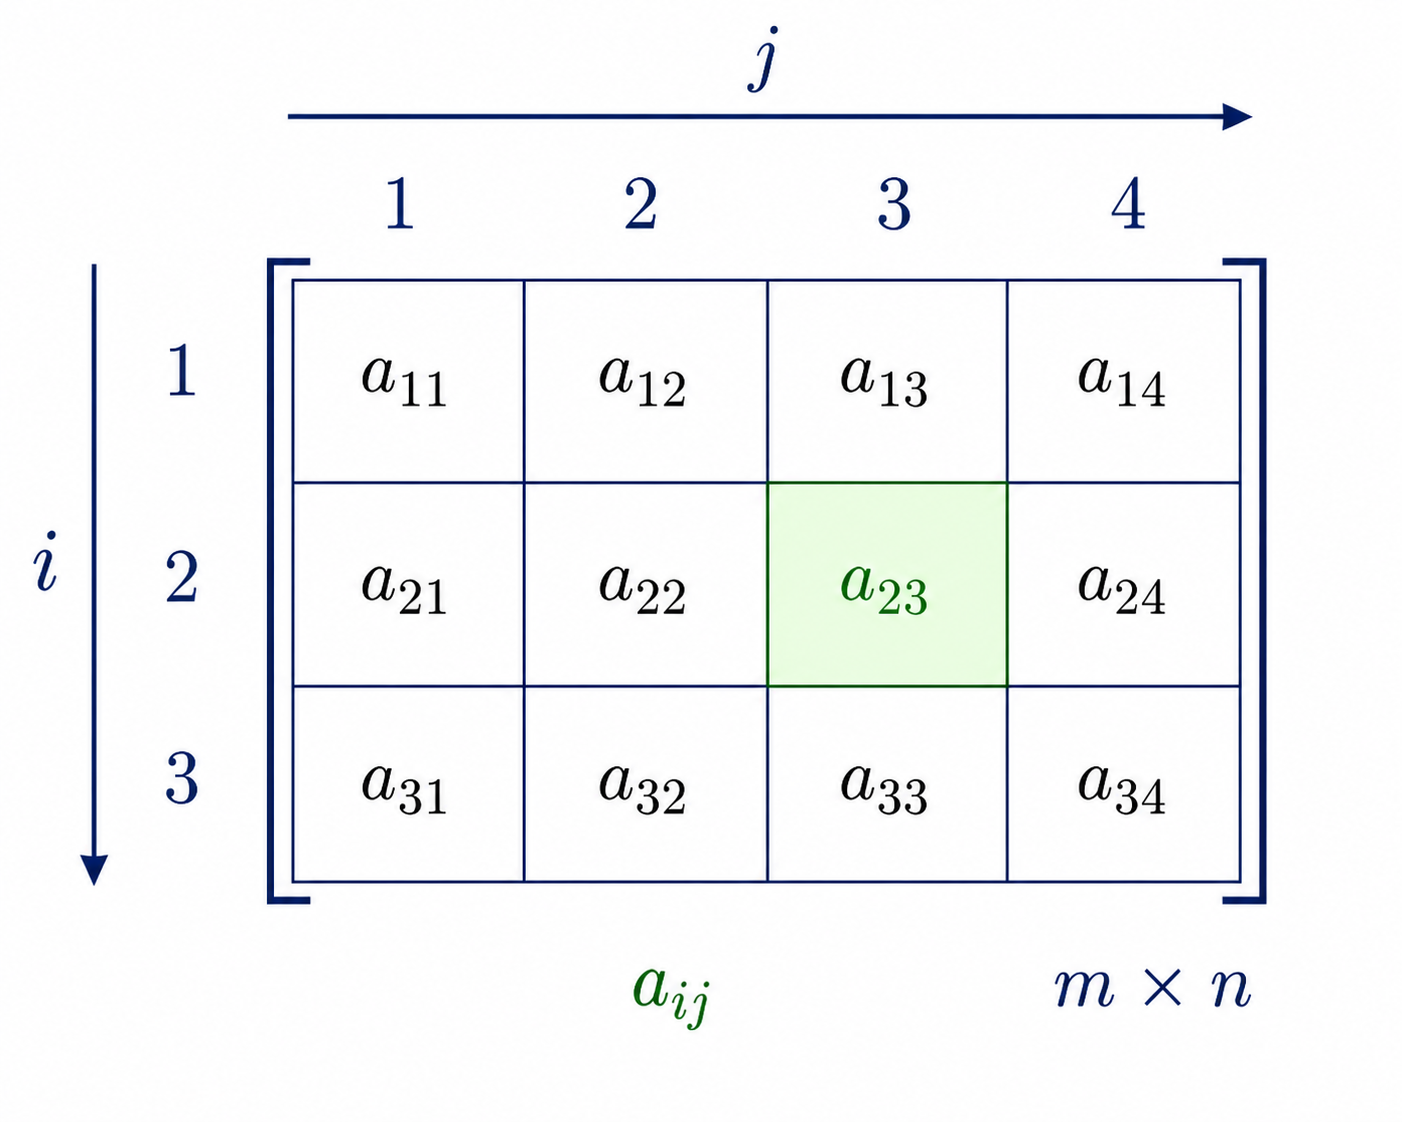
\includegraphics[width=0.62\textwidth]{Figures/png_ready/30-matrix-dimensions-manual.png}
    \caption{แผนภาพแสดงมิติของเมทริกซ์และตำแหน่งสมาชิก}
    \label{fig:matrix-dimensions}
\end{figure}

\begin{definition}[นิยามของเมทริกซ์]
\index{เมทริกซ์!นิยาม}
เมทริกซ์ คือการจัดเรียงข้อมูลในรูปแบบตารางสี่เหลี่ยมผืนผ้า ซึ่งประกอบด้วย $m$ แถว และ $n$ คอลัมน์ เมทริกซ์ขนาด $m \times n$ จะมีสมาชิกทั้งหมด $m \cdot n$ ตัว เขียนแทนด้วย
\[ A_{m \times n} = [a_{ij}]_{m \times n} \]
โดยที่ $a_{ij}$ คือสมาชิกที่อยู่ในแถวที่ $i$ และคอลัมน์ที่ $j$
\end{definition}

\begin{ex}
เมทริกซ์ $A = \begin{pmatrix} 1 & 2 & 3 \\ 4 & 5 & 6 \end{pmatrix}$ มีขนาด $2 \times 3$ (2 แถว 3 คอลัมน์)
\end{ex}
\begin{solution}
$a_{11}=1,\ a_{12}=2,\ a_{13}=3,\ a_{21}=4,\ a_{22}=5,\ a_{23}=6$ \solhere
\end{solution}

\begin{ex}
เมทริกซ์ $B = \begin{pmatrix} 1 & 2 \\ 3 & 4 \\ 5 & 6 \end{pmatrix}$ มีขนาด $3 \times 2$ (3 แถว 2 คอลัมน์)
\end{ex}
\begin{solution}
$B$ มี $3$ แถว ($\begin{psmallmatrix}1&2\end{psmallmatrix},\begin{psmallmatrix}3&4\end{psmallmatrix},\begin{psmallmatrix}5&6\end{psmallmatrix}$) และ $2$ คอลัมน์ $\therefore$ ขนาด $3\times 2$, สมาชิก $3\cdot 2 = 6$ ตัว \solhere
\end{solution}

เมทริกซ์ขนาด $m \times n$ สามารถเขียนในรูปทั่วไปได้ดังนี้

\[
A = \begin{pmatrix}
a_{11} & a_{12} & a_{13} & \cdots & a_{1n} \\
a_{21} & a_{22} & a_{23} & \cdots & a_{2n} \\
a_{31} & a_{32} & a_{33} & \cdots & a_{3n} \\
\vdots & \vdots & \vdots & \ddots & \vdots \\
a_{m1} & a_{m2} & a_{m3} & \cdots & a_{mn}
\end{pmatrix}
\]

\subsection{ประเภทของเมทริกซ์}
เมทริกซ์ในทางคณิตศาสตร์สามารถจำแนกออกได้เป็นหลายประเภทตามลักษณะการจัดเรียงตัวเลขและสมบัติเฉพาะตัวของสมาชิกภายใน โครงสร้างของเมทริกซ์จตุรัส เมทริกซ์ทแยงมุม เมทริกซ์เอกลักษณ์ หรือเมทริกซ์สมมาตร ล้วนมีบทบาทและรูปแบบการดำเนินการที่แตกต่างกันอย่างสิ้นเชิง การวิเคราะห์สมบัติเหล่านี้จะช่วยให้ผู้เรียนสามารถนำประเภทของเมทริกซ์ไปประยุกต์ใช้เพื่อลดความซับซ้อนของการคำนวณในขั้นตอนวิธีประเภทต่าง ๆ ได้อย่างเหมาะสม ดังภาพจำลองประเภทของเมทริกซ์ในรูปที่~\ref{fig:matrix-types}

\begin{figure}[H]
    \centering
    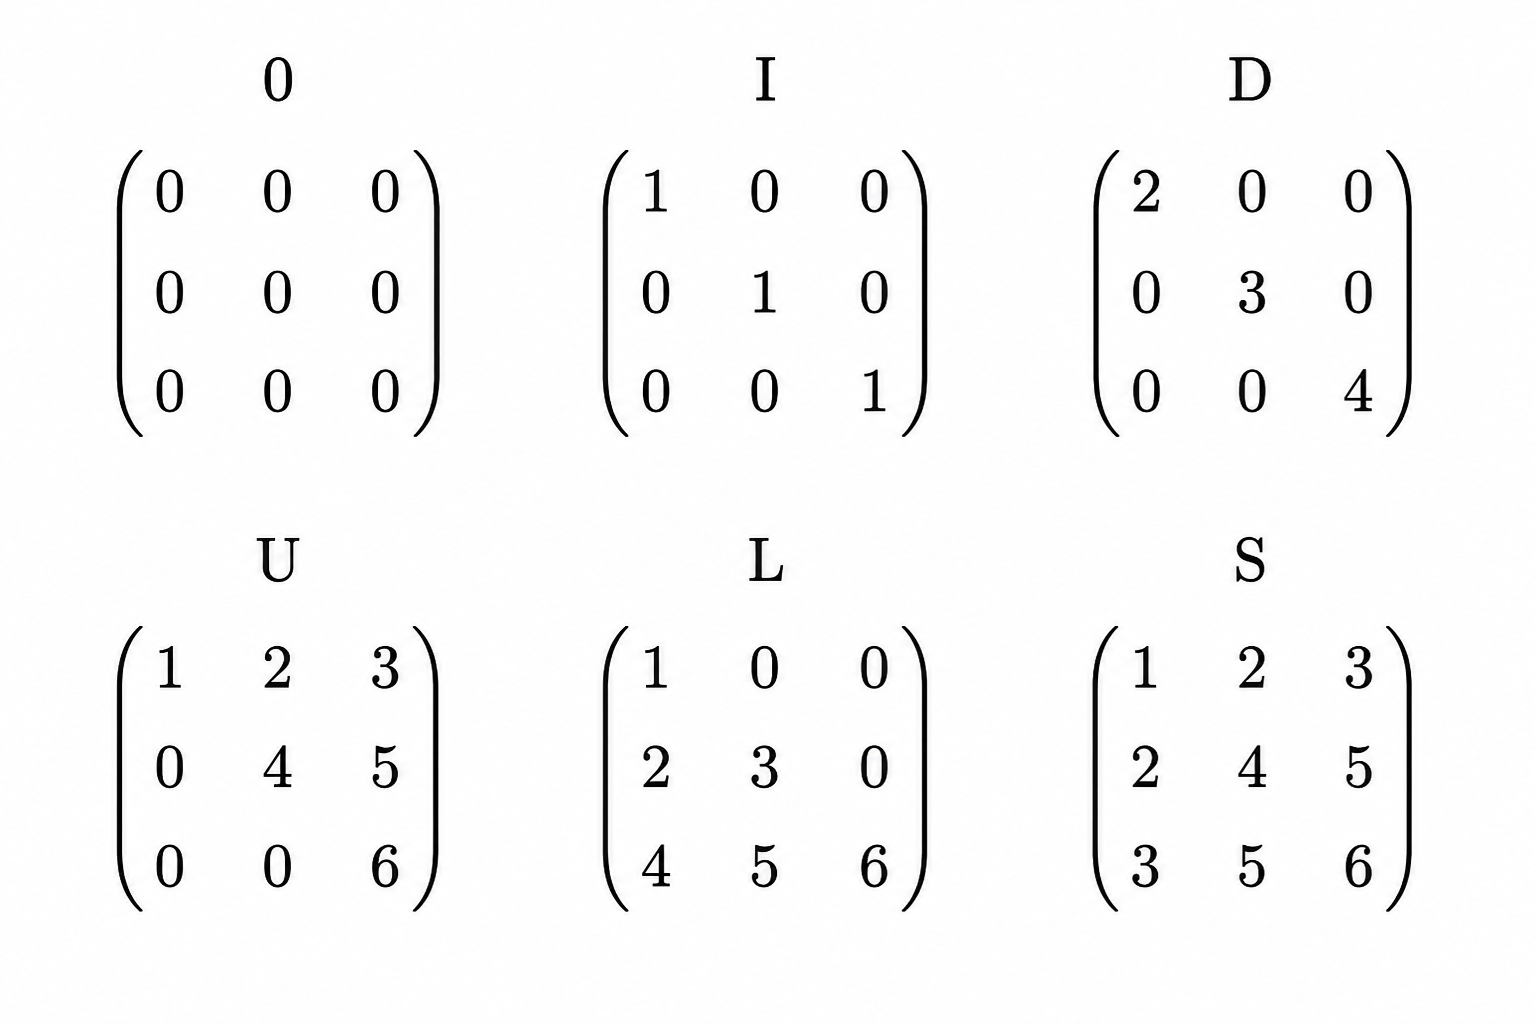
\includegraphics[width=0.62\textwidth]{Figures/png_ready/31-matrix-types-manual.png}
    \caption{แผนภาพแสดงประเภทของเมทริกซ์ที่สำคัญ}
    \label{fig:matrix-types}
\end{figure}

เมทริกซ์แต่ละประเภทมีคุณสมบัติเฉพาะที่แตกต่างกัน การจำแนกประเภทของเมทริกซ์ช่วยให้เข้าใจพฤติกรรมและการประยุกต์ใช้ในบริบททางคณิตศาสตร์และวิทยาการคอมพิวเตอร์ได้ชัดเจนขึ้น โดยเมทริกซ์จตุรัสเป็นประเภทที่สำคัญที่สุดเนื่องจากสามารถคำนวณดีเทอร์มิแนนต์และหาตัวผกผันได้

\begin{definition}[ประเภทของเมทริกซ์]
\index{เมทริกซ์!ประเภท}
เมทริกซ์ในทางคณิตศาสตร์จำแนกตามโครงสร้างและสมบัติเฉพาะของสมาชิกออกเป็นประเภทที่สำคัญ ได้แก่
\end{definition}

\begin{enumerate}
    \item เมทริกซ์ศูนย์ (Zero Matrix) $O_{m \times n}$ คือเมทริกซ์ที่ทุกสมาชิกเป็น 0
    
    \[O = \begin{pmatrix} 0 & 0 & 0 \\ 0 & 0 & 0 \end{pmatrix}\]
    \item เมทริกซ์แถว (Row Matrix) คือเมทริกซ์ที่มีเพียง 1 แถว ($1 \times n$)
    
    \[R = \begin{pmatrix} 1 & 2 & 3 & 4 \end{pmatrix}\]
    \item เมทริกซ์คอลัมน์ (Column Matrix) คือเมทริกซ์ที่มีเพียง 1 คอลัมน์ ($m \times 1$)
    
    \[C = \begin{pmatrix} 1 \\ 2 \\ 3 \end{pmatrix}\]
    \item เมทริกซ์จตุรัส (Square Matrix) คือเมทริกซ์ที่มีจำนวนแถวเท่ากับจำนวนคอลัมน์ ($n \times n$) เรียก $n$ ว่าขนาด (order) ของเมทริกซ์
    
    \[S = \begin{pmatrix} 1 & 2 \\ 3 & 4 \end{pmatrix}\quad (\text{ขนาด } 2 \times 2)\]

    \item เมทริกซ์ทแยงมุม (Diagonal Matrix) คือเมทริกซ์จตุรัสที่สมาชิกนอกเส้นทแยงมุมหลักเป็น 0 ทั้งหมด
    
    \[D = \begin{pmatrix} 1 & 0 & 0 \\ 0 & 2 & 0 \\ 0 & 0 & 3 \end{pmatrix}\]
    \item เมทริกซ์เอกลักษณ์ (Identity Matrix) $I_n$ คือเมทริกซ์ทแยงมุมที่สมาชิกบนเส้นทแยงมุมหลักเป็น 1 ทั้งหมด
    
    \[I_3 = \begin{pmatrix} 1 & 0 & 0 \\ 0 & 1 & 0 \\ 0 & 0 & 1 \end{pmatrix}\]
    \item เมทริกซ์สามเหลี่ยมบน (Upper Triangular Matrix) คือเมทริกซ์จตุรัสที่สมาชิกใต้เส้นทแยงมุมหลักเป็น 0
    
    \[U = \begin{pmatrix} 1 & 2 & 3 \\ 0 & 4 & 5 \\ 0 & 0 & 6 \end{pmatrix}\]
    \item เมทริกซ์สามเหลี่ยมล่าง (Lower Triangular Matrix) คือเมทริกซ์จตุรัสที่สมาชิกเหนือเส้นทแยงมุมหลักเป็น 0
    
    \[L = \begin{pmatrix} 1 & 0 & 0 \\ 2 & 3 & 0 \\ 4 & 5 & 6 \end{pmatrix}\]
    \item เมทริกซ์สมมาตร (Symmetric Matrix) คือเมทริกซ์จตุรัสที่มีคุณสมบัติ $a_{ij} = a_{ji}$ สำหรับทุก $i, j$
    
    \[S = \begin{pmatrix} 1 & 2 & 3 \\ 2 & 4 & 5 \\ 3 & 5 & 6 \end{pmatrix}\]
    \item เมทริกซ์เส้นทแยงมุมเฉียง (Skew-Symmetric Matrix) คือเมทริกซ์จตุรัสที่มีคุณสมบัติ $a_{ij} = -a_{ji}$ สำหรับทุก $i, j$ และ $a_{ii} = 0$
    
    \[K = \begin{pmatrix} 0 & 2 & -3 \\ -2 & 0 & 4 \\ 3 & -4 & 0 \end{pmatrix}\]
\end{enumerate}

\begin{ex}
เมทริกซ์สมมาตรและเมทริกซ์เส้นทแยงมุมเฉียงมีความสำคัญในการประยุกต์ เช่น ในทฤษฎีสถิติ เมทริกซ์ความแปรปรวน (covariance matrix) เป็นเมทริกซ์สมมาตร และในฟิสิกส์ เมทริกซ์เส้นทแยงมุมเฉียงใช้ในการแสดงปริมาณเวกเตอร์
\end{ex}
\begin{solution}
เมทริกซ์สมมาตร ($a_{ij}=a_{ji}$) พบในเมทริกซ์ความแปรปรวน (covariance); เมทริกซ์เส้นทแยงมุมเฉียง ($a_{ij}=-a_{ji},\ a_{ii}=0$) ใช้แทนปริมาณเวกเตอร์ เช่น ทอร์กในฟิสิกส์ $\therefore$ ทั้งสองชนิดช่วยลดความซับซ้อนของการคำนวณ \solhere
\end{solution}

\section{การดำเนินการระหว่างเมทริกซ์}
\label{sec:matrix-operations}
การประยุกต์ใช้เมทริกซ์ในทางปฏิบัติจำเป็นต้องมีนิยามการคำนวณทางพีชคณิตที่สอดคล้องกัน เพื่อแปลงข้อมูลหรือคำนวณค่าผลลัพธ์จากโครงสร้างข้อมูลสองมิตินี้ การดำเนินการพื้นฐานประกอบด้วยความเท่ากันของเมทริกซ์ การบวกและการลบเมทริกซ์ การคูณด้วยปริมาณสเกลาร์ ตลอดจนการคูณกันเองระหว่างสองเมทริกซ์ และการสลับเปลี่ยนแถวเป็นคอลัมน์ การดำเนินการแต่ละประเภทมีกฎเกณฑ์ เงื่อนไขข้อกำหนด และสมบัติทางคณิตศาสตร์ที่ผู้เรียนต้องเข้าใจเพื่อหลีกเลี่ยงความเข้าใจผิดในการวิเคราะห์ระบบ ดังรายละเอียดเชิงลึกและเงื่อนไขการคำนวณต่อไปนี้

\subsection{ความเท่ากันของเมทริกซ์}
ความสัมพันธ์ระดับพื้นฐานที่สุดระหว่างสองเมทริกซ์คือความเท่ากัน ซึ่งกำหนดเงื่อนไขทางโครงสร้างที่เข้มงวดสำหรับการเปรียบเทียบค่าข้อมูลในแต่ละตำแหน่ง การตรวจสอบความเท่ากันจะทำได้ก็ต่อเมื่อเมทริกซ์ทั้งสองมีมิติที่สอดคล้องกันอย่างสมบูรณ์ และค่าสมาชิกในทุกตำแหน่งตรงกันทุกประการ สมบัตินี้มักถูกนำไปใช้ในขั้นตอนวิธีการจับคู่ข้อมูล (Pattern Matching) และการคำนวณค่าตัวแปรในระบบสมการเชิงเส้น ดังนิยามต่อไปนี้
\begin{definition}[ความเท่ากันของเมทริกซ์]
\index{ความเท่ากันของเมทริกซ์!นิยาม}
เมทริกซ์ $A = [a_{ij}]$ และ $B = [b_{ij}]$ ขนาด $m \times n$ เท่ากัน ก็ต่อเมื่อ
\[ a_{ij} = b_{ij} \quad \forall i \in \{1,\ldots,m\}, j \in \{1,\ldots,n\} \]
\end{definition}

\begin{ex}
ถ้า $\begin{pmatrix} x & 2 \\ 3 & y \end{pmatrix} = \begin{pmatrix} 1 & 2 \\ 3 & 4 \end{pmatrix}$ แล้ว $x = 1$ และ $y = 4$
\end{ex}
\begin{solution}
\begin{align*}
(1,1):\ & x = 1\\
(2,2):\ & y = 4
\end{align*}
$\therefore x=1,\ y=4$ \solhere
\end{solution}

\subsection{การบวกและการลบเมทริกซ์}
การดำเนินการเพิ่มหรือลดระดับค่าของข้อมูลในตารางสองมิติมักทำผ่านการบวกและการลบเมทริกซ์ โดยมีเงื่อนไขพื้นฐานว่าเมทริกซ์คู่กรณีจะต้องมีขนาดมิติเท่ากันทุกประการเพื่อจะนำสมาชิกในตำแหน่งเดียวกันมาทำปฏิกิริยากันทางพีชคณิต หากขนาดมิติไม่เท่ากันจะไม่สามารถดำเนินการได้เนื่องจากจะไม่มีคู่สมาชิกมารองรับการรวมค่า ซึ่งผลลัพธ์จากการดำเนินการจะได้เมทริกซ์ใหม่ที่มีมิติคงเดิม ดังอธิบายตามบทนิยามและตัวอย่างต่อไปนี้

\begin{definition}[การบวกและการลบเมทริกซ์]
\index{การบวกเมทริกซ์!นิยาม}
\index{การลบเมทริกซ์!นิยาม}
กำหนดเมทริกซ์ $A = [a_{ij}]$ และ $B = [b_{ij}]$ ขนาด $m \times n$ การบวกและการลบเมทริกซ์กำหนดโดย
\[ A + B = [a_{ij} + b_{ij}] \quad\text{และ}\quad A - B = [a_{ij} - b_{ij}] \]
\end{definition}

หมายเหตุ: เมทริกซ์สองเมทริกซ์จะบวกหรือลบกันได้ก็ต่อเมื่อมีขนาดเท่ากัน

\begin{ex}
จงคำนวณผลลัพธ์ของการบวกและการลบเมทริกซ์ต่อไปนี้
\[
\begin{pmatrix} 1 & 2 & 3 \\ 4 & 5 & 6 \end{pmatrix} + \begin{pmatrix} 1 & 1 & 1 \\ 2 & 2 & 2 \end{pmatrix} = \;?
\]

\[
\begin{pmatrix} 5 & 6 \\ 7 & 8 \end{pmatrix} - \begin{pmatrix} 1 & 2 \\ 3 & 4 \end{pmatrix} = \;?
\]
\end{ex}
\begin{solution}
\begin{align*}
\begin{pmatrix} 1 & 2 & 3 \\ 4 & 5 & 6 \end{pmatrix} + \begin{pmatrix} 1 & 1 & 1 \\ 2 & 2 & 2 \end{pmatrix} &= \begin{pmatrix} 2 & 3 & 4 \\ 6 & 7 & 8 \end{pmatrix}\\
\begin{pmatrix} 5 & 6 \\ 7 & 8 \end{pmatrix} - \begin{pmatrix} 1 & 2 \\ 3 & 4 \end{pmatrix} &= \begin{pmatrix} 4 & 4 \\ 4 & 4 \end{pmatrix}
\end{align*}
\solhere
\end{solution}

\begin{ex}[สมบัติของการบวกเมทริกซ์]
สำหรับเมทริกซ์ $A, B, C$ ขนาด $m \times n$:
\begin{enumerate}
    \item $A + B = B + A$ \hfill (Commutative Law)
    \item $(A + B) + C = A + (B + C)$ \hfill (Associative Law)
    \item $A + O = A$ \hfill (Identity Law, $O$ คือเมทริกซ์ศูนย์)
    \item $A + (-A) = O$ \hfill (Inverse Law)
    \item $A - B = A + (-B)$
\end{enumerate}
\end{ex}
\begin{solution}
ทุกสมบัติลดรูปเป็นสมบัติการบวกจำนวนจริงรายตำแหน่ง
\begin{align*}
[A+B]_{ij} &= a_{ij}+b_{ij} = b_{ij}+a_{ij} = [B+A]_{ij}\\
[(A+B)+C]_{ij} &= a_{ij}+b_{ij}+c_{ij} = [A+(B+C)]_{ij}\\
[A+O]_{ij} &= a_{ij}+0 = a_{ij}\\
[A+(-A)]_{ij} &= a_{ij}-a_{ij} = 0
\end{align*}
$\therefore$ สลับที่ เปลี่ยนหมู่ เอกลักษณ์ ตรงข้าม เป็นจริง และ $A-B=A+(-B)$ \solhere
\end{solution}

\begin{ex}
การลบเมทริกซ์ไม่มีสมบัติการสลับที่ กล่าวคือ $A - B \neq B - A$ โดยทั่วไป
\end{ex}
\begin{solution}
ให้ $A = \begin{pmatrix} 1 & 2 \\ 3 & 4 \end{pmatrix}$, $B = \begin{pmatrix} 5 & 6 \\ 7 & 8 \end{pmatrix}$
\begin{align*}
A-B &= \begin{pmatrix} -4 & -4 \\ -4 & -4 \end{pmatrix}, \qquad
B-A = \begin{pmatrix} 4 & 4 \\ 4 & 4 \end{pmatrix}
\end{align*}
$\therefore A-B \neq B-A$ (การลบไม่มีสมบัติสลับที่) \solhere
\end{solution}

\subsection{การคูณเมทริกซ์ด้วยสเกลาร์}
การปรับขนาดหรือการขยายค่าของสมาชิกทุกตัวในเมทริกซ์อย่างสม่ำเสมอทำได้ด้วยการคูณด้วยปริมาณสเกลาร์หรือตัวเลขคงที่จำนวนจริง ค่าสเกลาร์จะถูกกระจายไปคูณกับสมาชิกในทุกตำแหน่งของเมทริกซ์อย่างไม่มีข้อยกเว้น ส่งผลให้ลักษณะเชิงโครงสร้างยังคงเดิมแต่มีขนาดของปริมาณเปลี่ยนแปลงไปตามสัดส่วนของสเกลาร์นั้น การดำเนินการนี้พบได้ทั่วไปในวิชากราฟิกส์คอมพิวเตอร์เมื่อมีการขยายภาพหรือปรับแต่งระดับความเข้มสี ดังรายละเอียดตามบทนิยามต่อไปนี้

\begin{definition}[การคูณเมทริกซ์ด้วยสเกลาร์]
\index{การคูณเมทริกซ์ด้วยสเกลาร์!นิยาม}
กำหนดเมทริกซ์ $A = [a_{ij}]$ ขนาด $m \times n$ และสเกลาร์ $c$ (ค่าคงตัวจำนวนจริง) การคูณสเกลาร์ $cA$ คือเมทริกซ์
\[ cA = [c \cdot a_{ij}] \]
\end{definition}

\begin{ex}
\[
3 \cdot \begin{pmatrix} 1 & 2 \\ 3 & 4 \end{pmatrix} = \begin{pmatrix} 3 & 6 \\ 9 & 12 \end{pmatrix}
\]
\end{ex}
\begin{solution}
\[
3\begin{pmatrix} 1 & 2 \\ 3 & 4 \end{pmatrix} = \begin{pmatrix} 3\cdot1 & 3\cdot2 \\ 3\cdot3 & 3\cdot4 \end{pmatrix} = \begin{pmatrix} 3 & 6 \\ 9 & 12 \end{pmatrix}
\]
\solhere
\end{solution}

\begin{ex}[สมบัติของการคูณสเกลาร์]
สำหรับเมทริกซ์ $A, B$ และสเกลาร์ $c, d$:
\begin{enumerate}
    \item $c(A + B) = cA + cB$ \hfill (Distributive Law)
    \item $(c + d)A = cA + dA$ \hfill (Distributive Law)
    \item $c(dA) = (cd)A$ \hfill (Associative Law)
    \item $1A = A$ \hfill (Identity Law)
    \item $0A = O$ \hfill (Zero Law)
\end{enumerate}
\end{ex}
\begin{solution}
ทุกสมบัติลดรูปเป็นสมบัติการคูณ/บวกจำนวนจริงรายตำแหน่ง
\begin{align*}
[c(A+B)]_{ij} &= c(a_{ij}+b_{ij}) = ca_{ij}+cb_{ij} = [cA+cB]_{ij}\\
[(c+d)A]_{ij} &= (c+d)a_{ij} = ca_{ij}+da_{ij} = [cA+dA]_{ij}\\
[c(dA)]_{ij} &= c(d\,a_{ij}) = (cd)a_{ij} = [(cd)A]_{ij}\\
[1A]_{ij} &= a_{ij}, \qquad [0A]_{ij} = 0
\end{align*}
$\therefore$ การกระจาย เปลี่ยนหมู่ เอกลักษณ์ ศูนย์ เป็นจริงทั้งหมด \solhere
\end{solution}

\subsection{การคูณเมทริกซ์ด้วยเมทริกซ์}
การดำเนินการคูณระหว่างเมทริกซ์ด้วยกันเองมีมิติความซับซ้อนที่สูงกว่าการดำเนินการอื่น ๆ เนื่องจากผลลัพธ์ไม่ได้เกิดจากการนำตำแหน่งเดียวกันมาคูณกันโดยตรง แต่ต้องอาศัยการจับคู่ผลรวมคูณสะสมระหว่างแถวของเมทริกซ์ตัวหน้ากับคอลัมน์ของเมทริกซ์ตัวหลัง เงื่อนไขสำคัญคือจำนวนคอลัมน์ของตัวตั้งจะต้องเท่ากับจำนวนแถวของตัวคูณพอดี จึงจะสามารถเกิดผลคูณสอดคล้อง (Conformable) ได้ การคูณเมทริกซ์ถูกใช้แสดงความเชื่อมโยงเชิงเส้นในแบบจำลองการแปลงรูปพิกเซลและโครงข่ายประสาทเทียม ดังแสดงลักษณะการทำงานในรูปที่~\ref{fig:matrix-multiplication}

\begin{figure}[H]
    \centering
    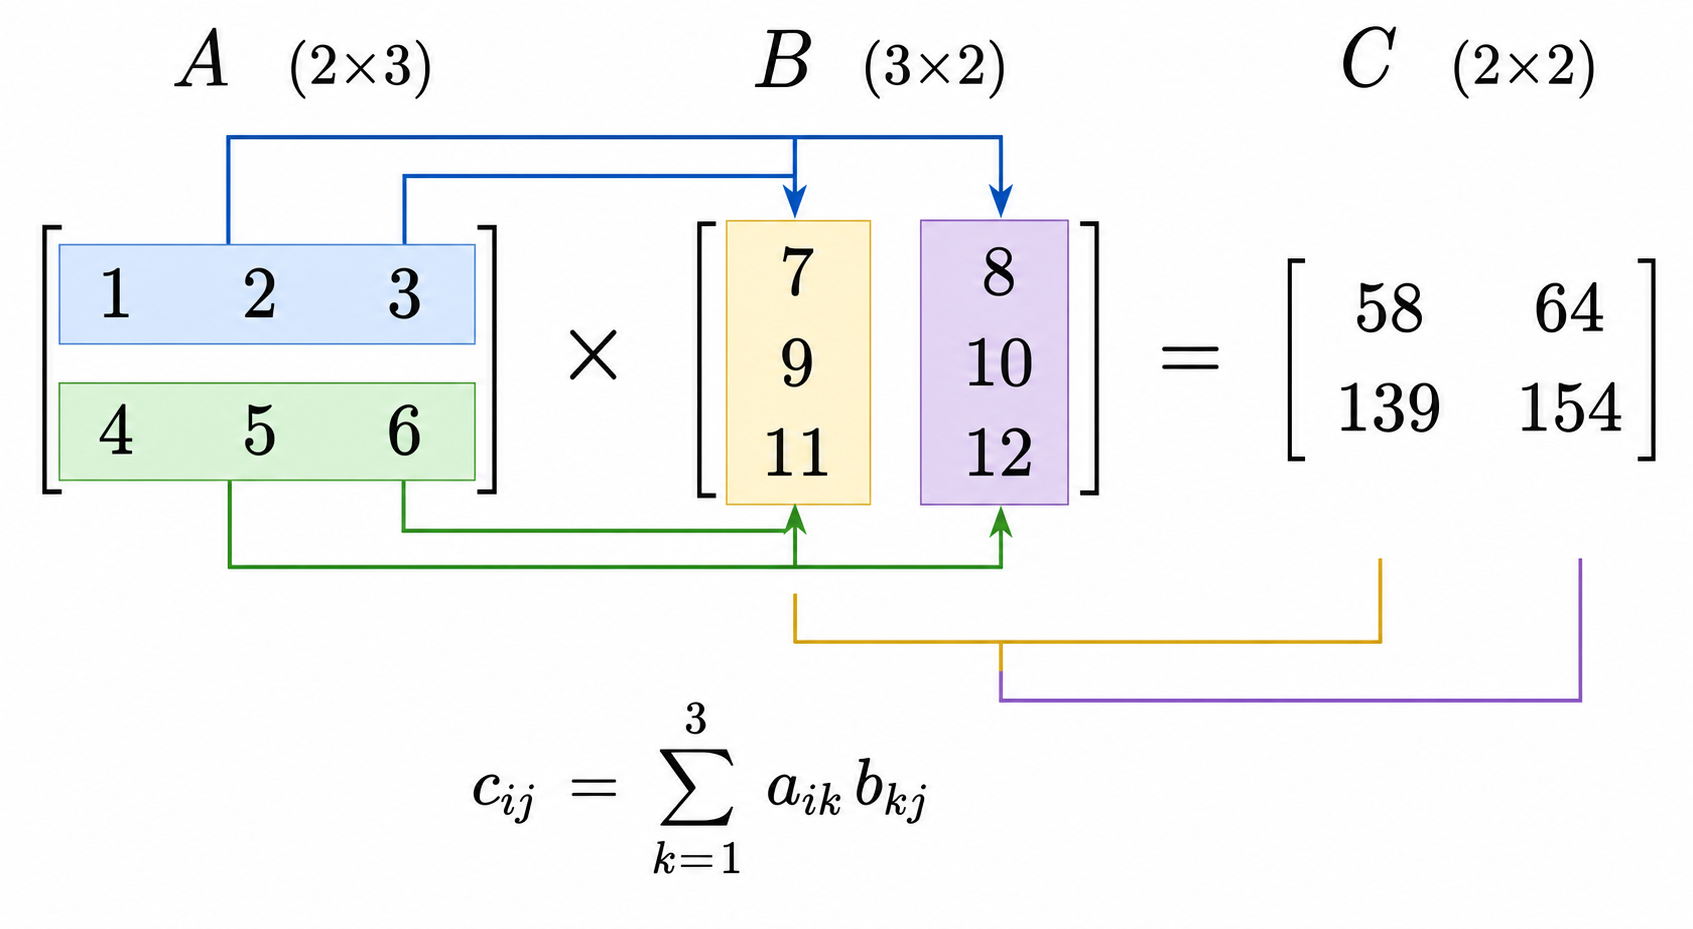
\includegraphics[width=0.62\textwidth]{Figures/png_ready/32-matrix-multiplication-manual.png}
    \caption{แผนภาพแสดงการคูณแถวของเมทริกซ์กับหลักของเมทริกซ์}
    \label{fig:matrix-multiplication}
\end{figure}

การคูณเมทริกซ์เป็นการดำเนินการที่ซับซ้อนกว่าการบวกและการคูณสเกลาร์ สมาชิกของเมทริกซ์ผลคูณคำนวณจากผลรวมของผลคูณของสมาชิกในแถวของเมทริกซ์ตัวแรกกับสมาชิกในคอลัมน์ของเมทริกซ์ตัวที่สอง การคูณเมทริกซ์สามารถมองได้ว่าเป็นการแทนการแปลงเชิงเส้น (linear transformation) ซึ่งใช้อย่างกว้างขวางในคณิตศาสตร์และวิทยาการคอมพิวเตอร์

\begin{definition}[การคูณเมทริกซ์ด้วยเมทริกซ์]
\index{การคูณเมทริกซ์!นิยาม}
กำหนดเมทริกซ์ $A = [a_{ij}]$ ขนาด $m \times n$ และเมทริกซ์ $B = [b_{jk}]$ ขนาด $n \times p$ ผลคูณ $AB$ จะได้เมทริกซ์ $C = [c_{ik}]$ ขนาด $m \times p$ โดยสมาชิกในแถวที่ $i$ คอลัมน์ที่ $k$ คือ
\[
c_{ik} = a_{i1}b_{1k} + a_{i2}b_{2k} + a_{i3}b_{3k} + \cdots + a_{in}b_{nk} = \sum_{j=1}^{n} a_{ij}b_{jk}
\]
\end{definition}

หมายเหตุ การคูณ $AB$ กระทำได้ก็ต่อเมื่อจำนวนคอลัมน์ของ $A$ เท่ากับจำนวนแถวของ $B$ (เรียกว่า conformable)

\begin{thrm}[สมบัติของการคูณเมทริกซ์]
สำหรับเมทริกซ์ $A, B, C$ ที่ขนาดเหมาะสม และสเกลาร์ $c$ การคูณเมทริกซ์มีสมบัติดังต่อไปนี้
\begin{enumerate}
    \item $(AB)C = A(BC)$ \hfill (Associative Law)
    \item $A(B + C) = AB + AC$ \hfill (Left Distributive Law)
    \item $(A + B)C = AC + BC$ \hfill (Right Distributive Law)
    \item $AI = IA = A$ \hfill (Identity Law, $I$ คือเมทริกซ์เอกลักษณ์)
    \item $c(AB) = (cA)B = A(cB)$ \hfill (Scalar Multiplication)
    \item $(AB)^T = B^T A^T$ \hfill (Transpose of Product)
\end{enumerate}
\end{thrm}

\begin{thrm}
สำหรับเมทริกซ์ $A$ และ $B$ ที่สามารถคูณกันได้ จะได้ว่า $(AB)^T = B^T A^T$
\end{thrm}

\begin{proof}
การพิสูจน์สมบัติ $(AB)^T = B^T A^T$ พิจารณาเปรียบเทียบสมาชิกในตำแหน่ง $(k,i)$ เป็นขั้นตอนดังนี้:
\begin{enumerate}[label=\textbf{\arabic*.}]
    \item \textbf{กำหนดเมทริกซ์ผลคูณ:} ให้ $A = [a_{ij}]$ และ $B = [b_{jk}]$ ให้ $C = AB$ เป็นเมทริกซ์ผลคูณ โดยมีสมาชิกตำแหน่ง $(i,k)$ คือ
    \[ c_{ik} = \sum_{j} a_{ij}b_{jk} \]
    
    \item \textbf{หาทรานสโพสของผลคูณ ($C^T$):} จากนิยามทรานสโพส สมาชิกในตำแหน่ง $(k,i)$ ของ $C^T$ คือ
    \[ (C^T)_{ki} = C_{ik} = \sum_{j} a_{ij}b_{jk} \]
    
    \item \textbf{หาผลคูณของทรานสโพสย้อนกลับ ($B^T A^T$):} สมาชิกในตำแหน่ง $(k,i)$ ของ $B^T A^T$ คือ
    \[ (B^T A^T)_{ki} = \sum_{j} (B^T)_{kj} (A^T)_{ji} = \sum_{j} b_{jk} a_{ij} \]
    
    \item \textbf{สรุปผลการสลับที่การคูณ:} เนื่องจาก $a_{ij}b_{jk} = b_{jk}a_{ij}$ เป็นสเกลาร์ที่สลับที่การคูณได้ ทำให้ $(C^T)_{ki} = (B^T A^T)_{ki}$ สำหรับทุกตำแหน่ง
\end{enumerate}
ดังนั้นจึงสรุปได้ว่า $(AB)^T = B^T A^T$
\end{proof}

\begin{ex}
จงหาผลคูณ $AB$ เมื่อ
\[
A = \begin{pmatrix} 1 & 2 \\ 3 & 4 \end{pmatrix}, \quad B = \begin{pmatrix} 5 & 6 \\ 7 & 8 \end{pmatrix}
\]
\end{ex}

\begin{solution}
$A_{2\times2}B_{2\times2}$ กระทำได้ ($c_{ik}=\sum_j a_{ij}b_{jk}$)
\begin{align*}
AB &= \begin{pmatrix} (1)(5)+(2)(7) & (1)(6)+(2)(8) \\ (3)(5)+(4)(7) & (3)(6)+(4)(8) \end{pmatrix}\\
&= \begin{pmatrix} 19 & 22 \\ 43 & 50 \end{pmatrix}
\end{align*}
\solhere
\end{solution}

\begin{ex}
จงคำนวณผลคูณ $AB$ และ $BA$ เมื่อ
\[
A = \begin{pmatrix} 1 & 2 & 3 \end{pmatrix}, \quad B = \begin{pmatrix} 4 \\ 5 \\ 6 \end{pmatrix}
\]
แล้วสังเกตว่าการคูณเมทริกซ์ไม่มีสมบัติสลับที่
\end{ex}
\begin{solution}
\begin{align*}
AB &= \begin{pmatrix} 1 & 2 & 3 \end{pmatrix}\begin{pmatrix} 4 \\ 5 \\ 6 \end{pmatrix} = [1(4)+2(5)+3(6)] = [32]\\
BA &= \begin{pmatrix} 4 \\ 5 \\ 6 \end{pmatrix}\begin{pmatrix} 1 & 2 & 3 \end{pmatrix} = \begin{pmatrix} 4 & 8 & 12 \\ 5 & 10 & 15 \\ 6 & 12 & 18 \end{pmatrix}
\end{align*}
$\therefore AB \neq BA$ (การคูณเมทริกซ์ไม่มีสมบัติสลับที่) \solhere
\end{solution}

\begin{ex}
จงหาผลคูณ $AB$ โดยที่ $A = \begin{pmatrix} 2 & 3 \\ 1 & 4 \end{pmatrix}$ และ $B = \begin{pmatrix} 5 & 2 \\ 1 & 6 \end{pmatrix}$
\end{ex}

\begin{solution}
\begin{align*}
AB &= \begin{pmatrix} (2)(5)+(3)(1) & (2)(2)+(3)(6) \\ (1)(5)+(4)(1) & (1)(2)+(4)(6) \end{pmatrix}\\
&= \begin{pmatrix} 13 & 22 \\ 9 & 26 \end{pmatrix}
\end{align*}
\solhere
\end{solution}

\begin{ex}
การคูณเมทริกซ์ไม่มีสมบัติการสลับที่ กล่าวคือ $AB \neq BA$ โดยทั่วไป นอกจากนี้ $AB = O$ ไม่ได้หมายความว่า $A = O$ หรือ $B = O$
\end{ex}
\begin{solution}
\textbf{ไม่สลับที่:} ให้ $A = \begin{pmatrix} 1 & 2 \\ 3 & 4 \end{pmatrix}$, $B = \begin{pmatrix} 5 & 6 \\ 7 & 8 \end{pmatrix}$
\[
AB = \begin{pmatrix} 19 & 22 \\ 43 & 50 \end{pmatrix} \neq \begin{pmatrix} 23 & 34 \\ 31 & 46 \end{pmatrix} = BA
\]
\textbf{$AB=O$ ไม่บังคับ $A=O$ หรือ $B=O$:} ให้ $A = \begin{pmatrix} 1 & 1 \\ 1 & 1 \end{pmatrix}$, $B = \begin{pmatrix} 1 & -1 \\ -1 & 1 \end{pmatrix}$
\[
AB = \begin{pmatrix} 0 & 0 \\ 0 & 0 \end{pmatrix} = O \quad\text{แต่}\quad A,B \neq O
\]
\solhere
\end{solution}

\begin{ex}[สมบัติของการคูณเมทริกซ์]
สำหรับเมทริกซ์ $A, B, C$ ที่ขนาดเหมาะสม และสเกลาร์ $c$:
\begin{enumerate}
    \item $(AB)C = A(BC)$ \hfill (Associative Law)
    \item $A(B + C) = AB + AC$ \hfill (Left Distributive Law)
    \item $(A + B)C = AC + BC$ \hfill (Right Distributive Law)
    \item $AI = IA = A$ \hfill (Identity Law, $I$ คือเมทริกซ์เอกลักษณ์)
    \item $c(AB) = (cA)B = A(cB)$ \hfill (Scalar Multiplication)
    \item $(AB)^T = B^T A^T$ \hfill (Transpose of Product)
\end{enumerate}
\end{ex}
\begin{solution}
สมบัติทั้งหกพิสูจน์ได้จากนิยาม $[AB]_{ik}=\sum_j a_{ij}b_{jk}$ และสมบัติของผลบวก/ผลคูณจำนวนจริง เช่น การเปลี่ยนหมู่
\[
[(AB)C]_{i\ell} = \sum_{j,k} a_{ij}b_{jk}c_{k\ell} = [A(BC)]_{i\ell}
\]
และการแจกแจง $A(B+C)=AB+AC$, เอกลักษณ์ $AI=IA=A$; ส่วน $(AB)^T=B^TA^T$ พิสูจน์ในตัวอย่างถัดไป $\therefore$ ทุกสมบัติเป็นจริง \solhere
\end{solution}

\begin{ex}
พิสูจน์ $(AB)^T = B^T A^T$
\end{ex}
\begin{solution}
\begin{align*}
[(AB)^T]_{ki} &= [AB]_{ik} = \sum_{j} a_{ij}b_{jk}\\
[B^T A^T]_{ki} &= \sum_{j} [B^T]_{kj}[A^T]_{ji} = \sum_{j} b_{jk}a_{ij} = \sum_{j} a_{ij}b_{jk}
\end{align*}
$\therefore [(AB)^T]_{ki} = [B^TA^T]_{ki}$ ทุก $(k,i)$ จึง $(AB)^T = B^TA^T$ \solhere
\end{solution}

\subsection{เมทริกซ์สลับเปลี่ยน (Transpose)}
เมทริกซ์สลับเปลี่ยนเป็นการดำเนินการพื้นฐานที่สลับโครงสร้างทิศทางของข้อมูล โดยเปลี่ยนแถวของเมทริกซ์ให้กลายเป็นคอลัมน์ และเปลี่ยนคอลัมน์ของเมทริกซ์ให้กลายเป็นแถวตามลำดับ สมบัตินี้ช่วยอำนวยความสะดวกในการวิเคราะห์สมบัติเชิงพีชคณิตเชิงเส้นเชิงลึก เช่น การคำนวณหาสมมาตรของเมทริกซ์ความแปรปรวนร่วมเกี่ยว ตลอดจนการหาตัวผกผันในปริภูมิของเมทริกซ์เชิงตั้งฉาก (Orthogonal Matrix) ดังรายละเอียดตามนิยามต่อไปนี้

\begin{definition}[เมทริกซ์สลับเปลี่ยน]
\index{เมทริกซ์สลับเปลี่ยน!นิยาม}
เมทริกซ์สลับเปลี่ยน ของเมทริกซ์ $A = [a_{ij}]$ ขนาด $m \times n$ คือเมทริกซ์
\[ A^T = [a_{ji}]_{n \times m} \]
ที่เกิดจากการสลับแถวเป็นคอลัมน์
\end{definition}

\begin{ex}
จงหา transpose ของเมทริกซ์ $A = \begin{pmatrix} 1 & 2 & 3 \\ 4 & 5 & 6 \end{pmatrix}$
\end{ex}
\begin{solution}
\[
A = \begin{pmatrix} 1 & 2 & 3 \\ 4 & 5 & 6 \end{pmatrix} \Rightarrow A^T = \begin{pmatrix} 1 & 4 \\ 2 & 5 \\ 3 & 6 \end{pmatrix} \quad (\text{ขนาด } 3\times 2)
\]
\solhere
\end{solution}

\begin{ex}[สมบัติของ Transpose]
สำหรับเมทริกซ์ $A, B$:
\begin{enumerate}
    \item $(A^T)^T = A$
    \item $(A + B)^T = A^T + B^T$
    \item $(cA)^T = cA^T$
    \item $(AB)^T = B^T A^T$
\end{enumerate}
\end{ex}
\begin{solution}
ทุกสมบัติตามนิยาม $[A^T]_{ij}=a_{ji}$
\begin{align*}
[(A^T)^T]_{ij} &= [A^T]_{ji} = a_{ij} \Rightarrow (A^T)^T = A\\
[(A+B)^T]_{ij} &= a_{ji}+b_{ji} = [A^T+B^T]_{ij}\\
[(cA)^T]_{ij} &= c\,a_{ji} = [cA^T]_{ij}
\end{align*}
$\therefore$ ทั้งสามเป็นจริง และ $(AB)^T=B^TA^T$ (พิสูจน์แล้วข้างต้น) \solhere
\end{solution}

\begin{thrm}
เมทริกซ์จตุรัส $A$ เป็นสมมาตร (Symmetric) ก็ต่อเมื่อ $A^T = A$ และเป็นเส้นทแยงมุมเฉียง (Skew-Symmetric) ก็ต่อเมื่อ $A^T = -A$
\end{thrm}

\begin{thrm}
ทุกเมทริกซ์จตุรัส $A$ สามารถเขียนได้ในรูปผลบวกของเมทริกซ์สมมาตรและเมทริกซ์เส้นทแยงมุมเฉียง ดังนี้

\[
A = \frac{1}{2}(A + A^T) + \frac{1}{2}(A - A^T)
\]
โดยที่ $\frac{1}{2}(A + A^T)$ เป็นเมทริกซ์สมมาตร เนื่องจาก $(\frac{1}{2}(A + A^T))^T = \frac{1}{2}(A + A^T)$ และ $\frac{1}{2}(A - A^T)$ เป็นเมทริกซ์เส้นทแยงมุมเฉียง เนื่องจาก $(\frac{1}{2}(A - A^T))^T = -\frac{1}{2}(A - A^T)$
\end{thrm}

\section{ดีเทอร์มิแนนต์ (Determinants)}
\label{sec:determinants}
ดีเทอร์มิแนนต์เป็นคุณลักษณะเฉพาะเชิงตัวเลขที่สำคัญยิ่งของเมทริกซ์จตุรัส ซึ่งทำหน้าที่สะท้อนสมบัติการเปลี่ยนขนาดของปริมาตรเมื่อมองเมทริกซ์ในฐานะการแปลงเชิงเส้น ค่าดีเทอร์มิแนนต์ช่วยระบุว่าเมทริกซ์นั้นมีตัวผกผันหรือไม่ และใช้เป็นค่าตัวหารหลักในสูตรการคำนวณต่าง ๆ ของการแก้ระบบสมการเชิงเส้น ในหัวข้อนี้ผู้เรียนจะได้ศึกษาความหมาย บทนิยามเชิงเลขคณิต สมบัติต่าง ๆ รวมถึงวิธีการคำนวณสำหรับเมทริกซ์ขนาดต่าง ๆ ดังต่อไปนี้

\subsection{นิยามของดีเทอร์มิแนนต์}
นิยามเชิงคณิตศาสตร์ของดีเทอร์มิแนนต์เริ่มต้นจากกรณีพื้นฐานขนาดมิติต่ำ ซึ่งช่วยสร้างความเข้าใจเชิงกลไกเกี่ยวกับการถ่วงน้ำหนักและการหักล้างกันของสมาชิกในทแยงมุมหลักและทแยงมุมรอง แผนภาพแสดงทิศทางการคูณตัวเลขทแยงมุมขึ้นลงสำหรับเมทริกซ์ขนาดสองคูณสอง จะเป็นรากฐานสำหรับสูตรการคำนวณที่ซับซ้อนขึ้นในมิติสูง ดังอธิบายและจำลองรายละเอียดในรูปที่~\ref{fig:determinant-2x2}

\begin{figure}[H]
    \centering
    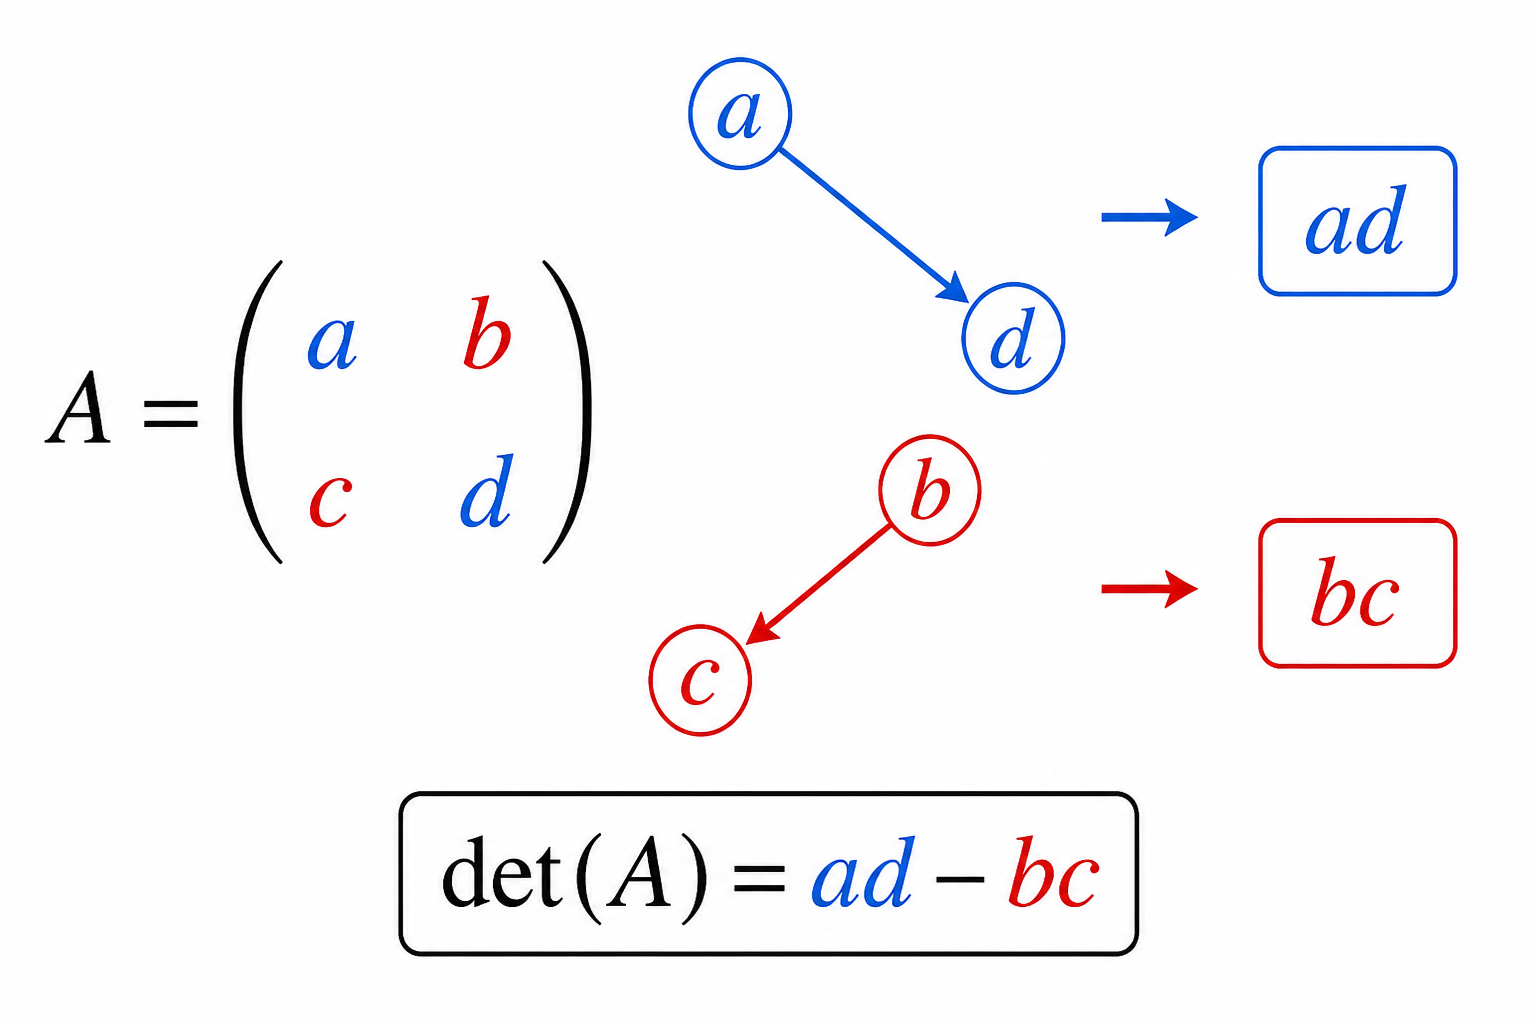
\includegraphics[width=0.62\textwidth]{Figures/png_ready/33-determinant-2x2-manual.png}
    \caption{แผนภาพแสดงดีเทอร์มิแนนต์ของเมทริกซ์ $2\times2$}
    \label{fig:determinant-2x2}
\end{figure}


\begin{definition}[ดีเทอร์มิแนนต์]
\index{ดีเทอร์มิแนนต์!นิยาม}
ดีเทอร์มิแนนต์ ของเมทริกซ์จตุรัส $A$ ขนาด $n \times n$ เขียนแทนด้วย $\det(A)$ หรือ $|A|$
\end{definition}

\begin{definition}[ดีเทอร์มิแนนต์ของเมทริกซ์ขนาดเล็ก]
ดีเทอร์มิแนนต์ของเมทริกซ์จตุรัสนิยามตามขนาดดังต่อไปนี้
\begin{enumerate}
  \item สำหรับเมทริกซ์ขนาด $1 \times 1$: $\det([a]) = a$
  \item สำหรับเมทริกซ์ขนาด $2 \times 2$:
  \[
    \det\begin{pmatrix} a & b \\ c & d \end{pmatrix} = ad - bc
  \]
  โดยที่ $a$ และ $d$ อยู่บนเส้นทแยงมุมหลัก ส่วน $b$ และ $c$ อยู่บนเส้นทแยงมุมรอง ดีเทอร์มิแนนต์คือผลคูณเส้นทแยงมุมหลักลบผลคูณเส้นทแยงมุมรอง
\end{enumerate}
\end{definition}

\begin{ex}
จงคำนวณ $\det\begin{pmatrix} 1 & 2 \\ 3 & 4 \end{pmatrix}$
\end{ex}
\begin{solution}
\[
\det\begin{pmatrix} 1 & 2 \\ 3 & 4 \end{pmatrix} = ad-bc = (1)(4)-(2)(3) = -2
\]
\solhere
\end{solution}

\begin{prop}[กฎของ Sarrus สำหรับเมทริกซ์ $3 \times 3$]
สำหรับเมทริกซ์ขนาด $3 \times 3$ สามารถคำนวณดีเทอร์มิแนนต์ได้โดยกฎของ Sarrus ดังนี้
\[
\det\begin{pmatrix} a & b & c \\ d & e & f \\ g & h & i \end{pmatrix} = aei + bfg + cdh - ceg - bdi - afh
\]
โดยเทอมบวก ($aei, bfg, cdh$) คือผลคูณตามเส้นทแยงมุมหลักและเส้นทแยงมุมขนาน และเทอมลบ ($ceg, bdi, afh$) คือผลคูณตามเส้นทแยงมุมรองและเส้นทแยงมุมขนาน
\end{prop}

\begin{ex}
จงคำนวณ $\det\begin{pmatrix} 1 & 2 & 3 \\ 4 & 5 & 6 \\ 7 & 8 & 9 \end{pmatrix}$ โดยใช้กฎของ Sarrus
\end{ex}
\begin{solution}
\begin{align*}
\det &= (1)(5)(9)+(2)(6)(7)+(3)(4)(8) - (3)(5)(7)-(2)(4)(9)-(1)(6)(8)\\
&= (45+84+96) - (105+72+48)\\
&= 225 - 225 = 0
\end{align*}
\solhere
\end{solution}

\begin{rem}
กฎของ Sarrus ใช้ได้เฉพาะกับเมทริกซ์ขนาด $3 \times 3$ เท่านั้น สำหรับเมทริกซ์ขนาดใหญ่กว่า ต้องใช้วิธีการอื่น เช่น cofactor expansion (กระจายตามแถวหรือคอลัมน์) หรือการลดรูปเมทริกซ์ (row reduction) ก่อนคำนวณดีเทอร์มิแนนต์
\end{rem}

\subsection{การกระจายโคแฟกเตอร์ (Cofactor Expansion)}
การขยายร่วมด้วยค่าโคแฟกเตอร์เป็นเทคนิคเชิงวิเคราะห์ระดับสากลในการลดระดับมิติของเมทริกซ์ขนาดใหญ่เพื่อคำนวณหาค่าดีเทอร์มิแนนต์ โดยทำการแยกเมทริกซ์ย่อย (Minor) ออกมาจากการตัดแถวและคอลัมน์ที่เลือก แล้วนำมาพิจารณาประกอบการคูณกับเครื่องหมายทิศทางตามดัชนีของตำแหน่งสมาชิก วิธีการนี้สามารถคำนวณกระจายตามแนวของแถวใดแถวหนึ่งหรือคอลัมน์ใดคอลัมน์หนึ่งได้โดยอิสระ โดยจะให้ค่าดีเทอร์มิแนนต์รวมที่เท่ากันเสมอ ดังขั้นตอนดังต่อไปนี้

\begin{definition}[Minor, Cofactor และ Cofactor Expansion]
กำหนดเมทริกซ์ $A = [a_{ij}]$ ขนาด $n \times n$
\begin{enumerate}
  \item Minor ของ $a_{ij}$ คือดีเทอร์มิแนนต์ของเมทริกซ์ย่อยที่ได้จากการลบแถว $i$ และคอลัมน์ $j$ เขียนแทนด้วย $M_{ij}$
  \item Cofactor ของ $a_{ij}$ คือ $C_{ij} = (-1)^{i+j} M_{ij}$
\end{enumerate}
ดีเทอร์มิแนนต์ของ $A$ สามารถคำนวณได้โดยการกระจายตามแถวที่ $i$:
\[
\det(A) = a_{i1}C_{i1} + a_{i2}C_{i2} + \cdots + a_{in}C_{in} = \sum_{j=1}^{n} a_{ij}C_{ij}
\]
หรือการกระจายตามคอลัมน์ที่ $j$:
\[
\det(A) = a_{1j}C_{1j} + a_{2j}C_{2j} + \cdots + a_{nj}C_{nj} = \sum_{i=1}^{n} a_{ij}C_{ij}
\]
\end{definition}

\begin{ex}
จงคำนวณ $\det\begin{pmatrix} 1 & 2 & 3 \\ 4 & 5 & 6 \\ 7 & 8 & 9 \end{pmatrix}$ โดยการกระจายตามแถวแรก
\end{ex}
\begin{solution}
\begin{align*}
M_{11} &= 45-48 = -3, & C_{11} &= (-1)^{2}(-3) = -3\\
M_{12} &= 36-42 = -6, & C_{12} &= (-1)^{3}(-6) = 6\\
M_{13} &= 32-35 = -3, & C_{13} &= (-1)^{4}(-3) = -3
\end{align*}
$\therefore \det(A) = 1(-3)+2(6)+3(-3) = -3+12-9 = 0$ \solhere
\end{solution}

\begin{ex}
คำนวณ $\det\begin{pmatrix} 2 & 1 & 3 \\ 0 & 4 & 1 \\ 5 & 6 & 0 \end{pmatrix}$ โดยการกระจายตามคอลัมน์ที่ 3
\end{ex}
\begin{solution}
\begin{align*}
M_{13} &= \det\begin{psmallmatrix} 0 & 4 \\ 5 & 6 \end{psmallmatrix} = -20, & C_{13} &= (-1)^{4}(-20) = -20\\
M_{23} &= \det\begin{psmallmatrix} 2 & 1 \\ 5 & 6 \end{psmallmatrix} = 7, & C_{23} &= (-1)^{5}(7) = -7\\
M_{33} &= \det\begin{psmallmatrix} 2 & 1 \\ 0 & 4 \end{psmallmatrix} = 8, & C_{33} &= (-1)^{6}(8) = 8
\end{align*}
$\therefore \det(A) = 3(-20)+1(-7)+0(8) = -67$ \solhere
\end{solution}

\begin{rem}[เคล็ดลับการเลือกแถว/คอลัมน์]
ในการคำนวณดีเทอร์มิแนนต์ ควรเลือกแถวหรือคอลัมน์ที่มีศูนย์มากที่สุด เพื่อลดจำนวนการคำนวณ ในตัวอย่างข้างต้น การกระจายตามคอลัมน์ที่ 3 มีสมาชิก $a_{33} = 0$ ทำให้มีเพียง 2 cofactor ที่ต้องคำนวณ การหลีกเลี่ยงการคำนวณ $C_{33}$ เป็นไปได้ทันทีเพราะพจน์ $a_{33}C_{33} = 0$ อยู่แล้ว
\end{rem}

\subsection{สมบัติของดีเทอร์มิแนนต์}
ดีเทอร์มิแนนต์มีสมบัติทางพีชคณิตที่สำคัญหลายประการ ซึ่งช่วยลดความซับซ้อนในการคำนวณได้อย่างมาก โดยไม่จำเป็นต้องใช้การกระจายโคแฟกเตอร์ที่มีความซับซ้อนระดับ $O(n!)$ ในทุกกรณี นอกจากนี้ สมบัติเหล่านี้ยังเป็นเครื่องมือหลักในการวิเคราะห์การมีอยู่ของเมทริกซ์ผกผัน การแก้ระบบสมการเชิงเส้น และการพิสูจน์ทฤษฎีบทในพีชคณิตเชิงเส้นขั้นสูง

\begin{thrm}[สมบัติพื้นฐานของดีเทอร์มิแนนต์]
\index{ดีเทอร์มิแนนต์!สมบัติพื้นฐาน}
กำหนดให้ $A$ และ $B$ เป็นเมทริกซ์จตุรัสขนาด $n \times n$ ดีเทอร์มิแนนต์มีสมบัติสำคัญดังต่อไปนี้:
\begin{enumerate}[leftmargin=1.8em,itemsep=0.3em]
    \item $\det(I) = 1$ โดยที่ $I$ คือเมทริกซ์เอกลักษณ์
    \item ถ้าเมทริกซ์ $A$ มีแถวหรือคอลัมน์ใดเป็นศูนย์ทั้งหมด จะได้ $\det(A) = 0$
    \item ถ้าสลับแถวสองแถว (หรือสลับคอลัมน์สองคอลัมน์) ค่าดีเทอร์มิแนนต์จะเปลี่ยนเป็นเครื่องหมายตรงข้าม
    \item ถ้าคูณแถวใดแถวหนึ่ง (หรือคอลัมน์ใดคอลัมน์หนึ่ง) ด้วยสเกลาร์ $c$ ค่าดีเทอร์มิแนนต์ใหม่จะเท่ากับ $c \det(A)$
    \item ถ้าคูณเมทริกซ์ทั้งเมทริกซ์ด้วยสเกลาร์ $c$ จะได้ $\det(cA) = c^n \det(A)$ สำหรับเมทริกซ์ขนาด $n \times n$
    \item ถ้าแถวหนึ่งเป็นผลรวมของสองพจน์ สามารถแยกดีเทอร์มิแนนต์ออกเป็นผลบวกของสองดีเทอร์มิแนนต์ได้
    \item $\det(AB) = \det(A)\det(B)$ \hfill (สมบัติการคูณดีเทอร์มิแนนต์)
    \item $\det(A^T) = \det(A)$ \hfill (ดีเทอร์มิแนนต์ของเมทริกซ์สลับเปลี่ยน)
    \item สำหรับเมทริกซ์สามเหลี่ยม (Upper/Lower Triangular Matrix) หรือเมทริกซ์เฉียง ค่า $\det(A) = a_{11} \cdot a_{22} \cdots a_{nn}$ (ผลคูณของสมาชิกบนเส้นทแยงมุมหลัก)
\end{enumerate}
\end{thrm}

\begin{proof}
พิสูจน์สำหรับเมทริกซ์ $2 \times 2$ ให้ $A = \begin{pmatrix} a & b \\ c & d \end{pmatrix}$ และ $B = \begin{pmatrix} e & f \\ g & h \end{pmatrix}$

การคูณเมทริกซ์ได้ $AB = \begin{pmatrix} ae+bg & af+bh \\ ce+dg & cf+dh \end{pmatrix}$

จากนิยามดีเทอร์มิแนนต์ของเมทริกซ์ $2\times 2$:
\begin{align}
\det(AB) &= (ae+bg)(cf+dh) - (af+bh)(ce+dg)
\end{align}

กระจายพจน์ทั้งสองชุดให้ครบ

\begin{align}
(ae+bg)(cf+dh) &= aecf + aedh + bgcf + bgdh \\
(af+bh)(ce+dg) &= afce + afdg + bhce + bhdg
\end{align}

ดังนั้น
\begin{align}
\det(AB) &= aecf + aedh + bgcf + bgdh - afce - afdg - bhce - bhdg
\end{align}

โดยสมบัติการสลับที่ของการคูณในจำนวนจริง $aecf = afce$ และ $bgdh = bhdg$ ดังนั้นพจน์
\[
aecf - afce = 0, \qquad bgdh - bhdg = 0
\]
เหลือพจน์ที่ไม่ตัดกัน 4 พจน์ ได้แก่
\begin{align}
\det(AB) &= aedh - afdg - bhce + bgcf \\
&= adeh - adfg - bceh + bcfg \\
&= ad(eh - fg) - bc(eh - fg) \\
&= (ad - bc)(eh - fg) \\
&= \det(A)\,\det(B)
\end{align}

สำหรับกรณีทั่วไป $n \times n$ การพิสูจน์ใช้หลักการของ cofactor expansion และ mathematical induction ซึ่งแสดงให้เห็นว่าสมบัติการคูณของดีเทอร์มิแนนต์เป็นจริงสำหรับทุกขนาดของเมทริกซ์จตุรัส
\end{proof}

\begin{ex}
\[
\det\begin{pmatrix} 2 & 0 & 0 \\ 0 & 3 & 0 \\ 0 & 0 & 5 \end{pmatrix} = 2 \times 3 \times 5 = 30
\]
\end{ex}
\begin{solution}
เมทริกซ์ทแยงมุม/สามเหลี่ยม $\Rightarrow \det = $ ผลคูณสมาชิกทแยงมุมหลัก
\[
\det\begin{pmatrix} 2 & 0 & 0 \\ 0 & 3 & 0 \\ 0 & 0 & 5 \end{pmatrix} = 2\cdot 3\cdot 5 = 30
\]
\solhere
\end{solution}

\begin{ex}
พิสูจน์ $\det(AB) = \det(A)\det(B)$ สำหรับเมทริกซ์ $2 \times 2$
\end{ex}
\begin{solution}
ให้ $A = \begin{psmallmatrix} a & b \\ c & d \end{psmallmatrix}$, $B = \begin{psmallmatrix} e & f \\ g & h \end{psmallmatrix} \Rightarrow AB = \begin{psmallmatrix} ae+bg & af+bh \\ ce+dg & cf+dh \end{psmallmatrix}$
\begin{align*}
\det(AB) &= (ae+bg)(cf+dh) - (af+bh)(ce+dg)\\
&= aedh + bgcf - afdg - bhce \quad (aecf,\,bgdh \text{ ตัดกัน})\\
&= ad(eh-fg) - bc(eh-fg)\\
&= (ad-bc)(eh-fg) = \det(A)\det(B)
\end{align*}
\solhere
\end{solution}

\begin{ex}[ตัวอย่างค้านสำหรับสมบัติการบวกดีเทอร์มิแนนต์]
จงแสดงตัวอย่างค้าน (counter-example) เพื่อพิสูจน์ว่า $\det(A + B) \neq \det(A) + \det(B)$ โดยทั่วไป
\end{ex}
\begin{solution}
เลือก $A = B = I_2 = \begin{pmatrix} 1 & 0 \\ 0 & 1 \end{pmatrix}$
จะได้ว่า
\begin{equation*}
  A + B = 2I_2 = \begin{pmatrix} 2 & 0 \\ 0 & 2 \end{pmatrix}
\end{equation*}
\begin{equation*}
  \det(A + B) = \det(2I_2) = (2)(2) - (0)(0) = 4
\end{equation*}
\begin{equation*}
  \det(A) + \det(B) = \det(I_2) + \det(I_2) = 1 + 1 = 2
\end{equation*}
เนื่องจาก $\det(A + B) = 4 \neq 2 = \det(A) + \det(B)$

ดังนั้น $\det(A + B) \neq \det(A) + \det(B)$ โดยทั่วไป (สมบัติการบวกดีเทอร์มิแนนต์ไม่เป็นไปตามกฎการแจกแจง) \solhere
\end{solution}

\begin{prop}[เงื่อนไขการมีตัวผกผัน]
เมทริกซ์จตุรัส $A$ จะมีตัวผกผันก็ต่อเมื่อ $\det(A) \neq 0$ ในกรณีนี้เรียก $A$ ว่า nonsingular หรือ invertible หากแต่ $\det(A) = 0$ จะเรียก $A$ ว่า singular หรือ noninvertible
\end{prop}

\section{ตัวผกผันของเมทริกซ์ (Matrix Inverse)}
\label{sec:matrix-inverse}
ตัวผกผันของเมทริกซ์หรืออินเวอร์สการคูณเป็นแนวคิดคณิตศาสตร์ที่มีลักษณะคล้ายคลึงกับตัวผกผันของจำนวนจริงที่เมื่อนำไปคูณกับจำนวนเดิมแล้วจะได้ผลลัพธ์เป็นหนึ่ง สำหรับเมทริกซ์จตุรัสใด ๆ ตัวผกผันการคูณจะมีสมบัติที่เมื่อนำไปคูณกับเมทริกซ์เดิมแล้วจะได้เมทริกซ์เอกลักษณ์เป็นผลลัพธ์ การหาตัวผกผันมีความสำคัญในทางวิทยาการคอมพิวเตอร์และการคำนวณทางวิศวกรรม เนื่องจากเป็นส่วนประกอบหลักในการประมวลผลคำตอบของสมการเมทริกซ์และแก้ปัญหาโครงข่ายสัญญาณประเภทต่างๆ ดังบทนิยามและขั้นตอนการคำนวณต่อไปนี้

\begin{definition}[ตัวผกผันของเมทริกซ์]
\index{ตัวผกผันของเมทริกซ์!นิยาม}
กำหนดเมทริกซ์จตุรัส $A$ ขนาด $n \times n$ ถ้ามีเมทริกซ์ $B$ ที่ทำให้
\[ AB = BA = I_n \]
แล้วจะเรียก $B$ ว่า ตัวผกผัน ของ $A$ เขียนแทนด้วย $A^{-1}$ และเรียก $A$ ว่าเป็นเมทริกซ์ที่มีตัวผกผัน แต่ถ้าไม่มีเมทริกซ์ $B$ ดังกล่าว จะเรียก $A$ ว่าเป็นเมทริกซ์ไม่มีตัวผกผัน
\end{definition}

\begin{prop}[{สูตรตัวผกผันของเมทริกซ์ $2\times 2$}]
สำหรับเมทริกซ์ $A = \begin{pmatrix} a & b \\ c & d \end{pmatrix}$ ที่มี $ad-bc \neq 0$ ตัวผกผันมีสูตรปิดดังต่อไปนี้
\[
A^{-1} = \frac{1}{ad-bc} \begin{pmatrix} d & -b \\ -c & a \end{pmatrix}
\]
\end{prop}

\begin{rem}[ขั้นตอนการใช้สูตร]
\begin{enumerate}
    \item คำนวณ $\det(A) = ad - bc$ ก่อนเสมอ และตรวจสอบว่า $\det(A) \neq 0$ ถ้า $\det(A) = 0$ แล้วเมทริกซ์ไม่มีตัวผกผัน
    \item สลับตำแหน่ง $a$ กับ $d$ (สมาชิกบนเส้นทแยงมุมหลักสลับกัน)
    \item เปลี่ยนเครื่องหมาย $b$ และ $c$ (เป็น $-b$ และ $-c$)
    \item คูณด้วย $\dfrac{1}{\det(A)}$
\end{enumerate}
\end{rem}

\begin{ex}
จงหาตัวผกผันของ $A = \begin{pmatrix} 1 & 2 \\ 3 & 4 \end{pmatrix}$
\end{ex}

\begin{solution}
\begin{align*}
\det(A) &= (1)(4)-(2)(3) = -2 \neq 0\\
A^{-1} &= \frac{1}{-2}\begin{pmatrix} 4 & -2 \\ -3 & 1 \end{pmatrix} = \begin{pmatrix} -2 & 1 \\ \tfrac{3}{2} & -\tfrac{1}{2} \end{pmatrix}
\end{align*}
ตรวจสอบ:
\[
AA^{-1} = \begin{pmatrix} 1 & 2 \\ 3 & 4 \end{pmatrix}\begin{pmatrix} -2 & 1 \\ \tfrac{3}{2} & -\tfrac{1}{2} \end{pmatrix} = \begin{pmatrix} 1 & 0 \\ 0 & 1 \end{pmatrix} = I
\]
\solhere
\end{solution}

\begin{ex}
จงหาตัวผกผันของ $A = \begin{pmatrix} 3 & 2 \\ 5 & 3 \end{pmatrix}$
\end{ex}

\begin{solution}
\begin{align*}
\det(A) &= (3)(3)-(2)(5) = -1 \neq 0\\
A^{-1} &= \frac{1}{-1}\begin{pmatrix} 3 & -2 \\ -5 & 3 \end{pmatrix} = \begin{pmatrix} -3 & 2 \\ 5 & -3 \end{pmatrix}
\end{align*}
ตรวจสอบ:
\[
AA^{-1} = \begin{pmatrix} 3 & 2 \\ 5 & 3 \end{pmatrix}\begin{pmatrix} -3 & 2 \\ 5 & -3 \end{pmatrix} = \begin{pmatrix} 1 & 0 \\ 0 & 1 \end{pmatrix} = I
\]
\solhere
\end{solution}

\begin{ex}
หาตัวผกผันของ $A = \begin{pmatrix} 2 & 1 & 1 \\ 0 & 1 & 1 \\ 1 & 0 & 1 \end{pmatrix}$
\end{ex}
\begin{solution}
\begin{align*}
\det(A) &= 2(1-0)-1(0-1)+1(0-1) = 2\\
C_{11},C_{12},C_{13} &= 1,\ 1,\ -1\\
C_{21},C_{22},C_{23} &= -1,\ 1,\ 1\\
C_{31},C_{32},C_{33} &= 0,\ -2,\ 2\\
\operatorname{adj}(A) &= [C_{ij}]^T = \begin{pmatrix} 1 & -1 & 0 \\ 1 & 1 & 1 \\ -1 & -2 & 2 \end{pmatrix}\\
A^{-1} &= \tfrac{1}{2}\operatorname{adj}(A) = \begin{pmatrix} \tfrac{1}{2} & -\tfrac{1}{2} & 0 \\ \tfrac{1}{2} & \tfrac{1}{2} & \tfrac{1}{2} \\ -\tfrac{1}{2} & -1 & 1 \end{pmatrix}
\end{align*}
\solhere
\end{solution}

\begin{ex}[สมบัติของตัวผกผัน]
สำหรับเมทริกซ์ invertible $A, B$ สรุปสมบัติที่สำคัญได้ดังนี้
\end{ex}
\begin{solution}
\begin{align*}
(A^{-1})^{-1} &= A\\
(AB)^{-1} &= B^{-1}A^{-1} && (\text{จาก } (AB)(B^{-1}A^{-1})=I)\\
(A^T)^{-1} &= (A^{-1})^T\\
\det(A^{-1}) &= \frac{1}{\det(A)} && (\text{จาก } \det(A)\det(A^{-1})=\det(I)=1)
\end{align*}
\solhere
\end{solution}

\begin{ex}
$(AB)^{-1} = B^{-1} A^{-1}$ ไม่ใช่ $A^{-1} B^{-1}$ ต้องระวังลำดับการคูณ!
\end{ex}
\begin{solution}
\begin{align*}
(AB)(B^{-1}A^{-1}) &= A(BB^{-1})A^{-1} = AIA^{-1} = I\\
(B^{-1}A^{-1})(AB) &= B^{-1}(A^{-1}A)B = B^{-1}IB = I
\end{align*}
$\therefore (AB)^{-1} = B^{-1}A^{-1}$ (ลำดับสลับกัน ไม่ใช่ $A^{-1}B^{-1}$) \solhere
\end{solution}

\begin{thrm}
สำหรับเมทริกซ์ invertible $A$ และ $B$ ตัวผกผันมีสมบัติดังต่อไปนี้
\end{thrm}

\begin{enumerate}
    \item $(A^{-1})^{-1} = A$ \hfill (ตัวผกผันของตัวผกผันคือตัวมันเอง)
    \item $(AB)^{-1} = B^{-1} A^{-1}$ \hfill (ตัวผกผันของผลคูณเท่ากับผลคูณของตัวผกผันในลำดับกลับกัน)
    \item $(A^T)^{-1} = (A^{-1})^T$ \hfill (ตัวผกผันของ transpose เท่ากับ transpose ของตัวผกผัน)
    \item $\det(A^{-1}) = \frac{1}{\det(A)}$ \hfill (ดีเทอร์มิแนนต์ของตัวผกผันเท่ากับส่วนกลับของดีเทอร์มิแนนต์)
\end{enumerate}

\begin{thrm}
$(AB)^{-1} = B^{-1} A^{-1}$ สำหรับเมทริกซ์ invertible $A$ และ $B$
\end{thrm}

\begin{prop}
$(AB)^{-1} = B^{-1} A^{-1}$ ไม่ใช่ $A^{-1} B^{-1}$ ต้องระวังลำดับการคูณเป็นอย่างยิ่ง เนื่องจากการคูณเมทริกซ์ไม่มีสมบัติการสลับที่
\end{prop}

\begin{cor}
ข้อควรระวังในการใช้ตัวผกผัน: สำหรับเมทริกซ์ $n \times n$ invertible ทั้งหมด จะได้ว่า $(A^{-1})^{-1} = A$ และ $(A^T)^{-1} = (A^{-1})^T$
\end{cor}

\section{ระบบสมการเชิงเส้น (Systems of Linear Equations)}
\label{sec:linear-systems}
การแก้ระบบสมการเชิงเส้นพร้อมกันหลายตัวแปรเป็นปัญหาพื้นฐานในหลากหลายสาขาวิชา ทั้งทางฟิสิกส์ วิศวกรรม และวิทยาการคอมพิวเตอร์ การนำระบบสมการมาจัดให้อยู่ในรูปของสมการเมทริกซ์ช่วยให้เราสามารถประยุกต์ใช้ทฤษฎีบททางพีชคณิตเชิงเส้นและขั้นตอนวิธีเชิงตัวเลขในการคำนวณหาคำตอบได้อย่างมีประสิทธิภาพและเป็นระบบ โดยผู้เรียนจะได้ศึกษาขอบเขตวิธีการแก้ระบบสมการผ่านตัวผกผันเมทริกซ์ กฎของคราเมอร์ และการกำจัดแบบเกาส์ ดังรายละเอียดต่อไปนี้

\subsection{การเขียนระบบสมการในรูปเมทริกซ์}
การแปลงความสัมพันธ์เชิงสมการที่แยกเป็นหลายสมการทางตรรกศาสตร์ให้อยู่ในรูปของประพจน์เมทริกซ์เดียว ช่วยเพิ่มความสะดวกในการวิเคราะห์โครงสร้างโดยใช้คอมพิวเตอร์ การแปลงนี้จัดกลุ่มตัวแปร สัมประสิทธิ์ และผลเฉลยออกเป็นเมทริกซ์สัมประสิทธิ์ เวกเตอร์ตัวแปร และเวกเตอร์คงที่ตามลำดับ ทำให้กระบวนการแปลงค่าและประมวลผลเชิงเส้นทำได้อย่างสอดคล้องรัดกุม ดังตัวอย่างการนำเสนอดังต่อไปนี้

\begin{ex}
ระบบสมการเชิงเส้น $n$ ตัวแปร $m$ สมการ สามารถเขียนในรูปเมทริกซ์ได้ดังนี้
\[
\begin{pmatrix}
a_{11} & a_{12} & \cdots & a_{1n} \\
a_{21} & a_{22} & \cdots & a_{2n} \\
\vdots & \vdots & \ddots & \vdots \\
a_{m1} & a_{m2} & \cdots & a_{mn}
\end{pmatrix}
\begin{pmatrix} x_1 \\ x_2 \\ \vdots \\ x_n \end{pmatrix}
=
\begin{pmatrix} b_1 \\ b_2 \\ \vdots \\ b_m \end{pmatrix}
\]
\end{ex}
\begin{solution}
เมทริกซ์สัมประสิทธิ์ $A$, เวกเตอร์ตัวแปร $x$, เวกเตอร์ค่าคงตัว $b$
\[
A = [a_{ij}]_{m\times n},\quad x = \begin{pmatrix} x_1 \\ \vdots \\ x_n \end{pmatrix},\quad b = \begin{pmatrix} b_1 \\ \vdots \\ b_m \end{pmatrix} \ \Rightarrow\ Ax = b
\]
\solhere
\end{solution}

\begin{ex}
ระบบสมการ ดังนี้

\[
\begin{aligned}
x + 2y + 3z &= 14 \\
2x + 3y + z &= 10 \\
3x + y + 2z &= 14
\end{aligned}
\]

เขียนในรูปเมทริกซ์ได้เป็น

\[
\begin{pmatrix} 1 & 2 & 3 \\ 2 & 3 & 1 \\ 3 & 1 & 2 \end{pmatrix} \begin{pmatrix} x \\ y \\ z \end{pmatrix} = \begin{pmatrix} 14 \\ 10 \\ 14 \end{pmatrix}
\]
\end{ex}
\begin{solution}
\[
\underbrace{\begin{pmatrix} 1 & 2 & 3 \\ 2 & 3 & 1 \\ 3 & 1 & 2 \end{pmatrix}}_{A} \underbrace{\begin{pmatrix} x \\ y \\ z \end{pmatrix}}_{x} = \underbrace{\begin{pmatrix} 14 \\ 10 \\ 14 \end{pmatrix}}_{b}
\]
$\therefore Ax = b$ \solhere
\end{solution}

\subsection{การแก้ระบบสมการโดยใช้ตัวผกผันเมทริกซ์}
วิธีการแรกในการหารายชื่อตัวแปรผลเฉลยของระบบสมการเชิงเส้นคือการใช้สมบัติความสัมพันธ์ของตัวผกผันเมทริกซ์เชิงคูณ โดยหากกำหนดให้ระบบสมการเขียนอยู่ในรูปสมการเมทริกซ์ $Ax = b$ และพบว่าเมทริกซ์สัมประสิทธิ์ $A$ มีคุณสมบัติการมีตัวผกผัน ($\det(A) \neq 0$) เราจะสามารถย้ายข้างคำนวณโดยคูณเมทริกซ์ผกผันเข้ากับเวกเตอร์ค่าคงตัวเพื่อหาผลเฉลยได้ทันที ดังรายละเอียดทฤษฎีบทและตัวอย่างดังต่อไปนี้

\begin{ex}
ถ้า $A$ มีตัวผกผัน ($Ax = b$) แล้ว $x = A^{-1}b$
\end{ex}
\begin{solution}
\begin{align*}
Ax &= b\\
A^{-1}Ax &= A^{-1}b\\
Ix = x &= A^{-1}b
\end{align*}
\solhere
\end{solution}

\begin{ex}
แก้ระบบสมการโดยใช้ตัวผกผัน:
\[
\begin{aligned}
x + 2y &= 5 \\
3x + 4y &= 11
\end{aligned}
\]
\end{ex}
\begin{solution}
$A = \begin{psmallmatrix} 1 & 2 \\ 3 & 4 \end{psmallmatrix}$, $b = \begin{psmallmatrix} 5 \\ 11 \end{psmallmatrix}$, $\det(A) = -2 \neq 0$
\begin{align*}
A^{-1} &= \frac{1}{-2}\begin{pmatrix} 4 & -2 \\ -3 & 1 \end{pmatrix} = \begin{pmatrix} -2 & 1 \\ \tfrac{3}{2} & -\tfrac{1}{2} \end{pmatrix}\\
x &= A^{-1}b = \begin{pmatrix} -2 & 1 \\ \tfrac{3}{2} & -\tfrac{1}{2} \end{pmatrix}\begin{pmatrix} 5 \\ 11 \end{pmatrix} = \begin{pmatrix} 1 \\ 2 \end{pmatrix}
\end{align*}
$\therefore x=1,\ y=2$ \solhere
\end{solution}

\subsection{การแก้ระบบสมการโดยใช้กฎของคราเมอร์ (Cramer's Rule)}
กฎของคราเมอร์เป็นกระบวนการหาคำตอบของระบบสมการเชิงเส้นโดยพึ่งพาการคำนวณอัตราส่วนค่าดีเทอร์มิแนนต์ของเมทริกซ์ย่อยที่ถูกแทนที่ด้วยเวกเตอร์คำตอบ วิธีการนี้ช่วยให้สามารถระบุค่าของตัวแปรใดตัวแปรหนึ่งได้โดยตรงโดยไม่ต้องคำนวณหาค่าตัวแปรตัวอื่นพร้อมกัน เหมาะสำหรับระบบสมการขนาดเล็กที่มีดีเทอร์มิแนนต์ของเมทริกซ์สัมประสิทธิ์ไม่เป็นศูนย์ ดังทฤษฎีบทการแปลงคณิตศาสตร์ต่อไปนี้

\begin{ex}[กฎของคราเมอร์]
สำหรับระบบสมการเชิงเส้น $Ax = b$ โดยที่ $A$ ขนาด $n \times n$ และ $\det(A) \neq 0$ คำตอบคือ
\[
x_i = \frac{\det(A_i)}{\det(A)}
\]
โดยที่ $A_i$ คือเมทริกซ์ที่ได้จากการแทนคอลัมน์ที่ $i$ ของ $A$ ด้วยเวกเตอร์ $b$
\end{ex}
\begin{solution}
\[
\det(A) \neq 0; \quad A_i = (A \text{ แทนคอลัมน์ } i \text{ ด้วย } b); \quad x_i = \frac{\det(A_i)}{\det(A)}
\]
\solhere
\end{solution}

\begin{ex}
แก้ระบบโดยใช้กฎของคราเมอร์

\[
\begin{aligned}
x + 2y &= 5 \\
3x + 4y &= 11
\end{aligned}
\]
\end{ex}
\begin{solution}
\begin{align*}
\det(A) &= 1(4)-2(3) = -2\\
x &= \frac{\det(A_1)}{\det(A)} = \frac{\det\begin{psmallmatrix} 5 & 2 \\ 11 & 4 \end{psmallmatrix}}{-2} = \frac{20-22}{-2} = 1\\
y &= \frac{\det(A_2)}{\det(A)} = \frac{\det\begin{psmallmatrix} 1 & 5 \\ 3 & 11 \end{psmallmatrix}}{-2} = \frac{11-15}{-2} = 2
\end{align*}
$\therefore x=1,\ y=2$ \solhere
\end{solution}

\begin{ex}
กฎของคราเมอร์มีประสิทธิภาพในการแสดงทฤษฎี แต่ในทางปฏิบัติ หากคำนวณดีเทอร์มิแนนต์ด้วย cofactor expansion แบบตรงไปตรงมา ความซับซ้อนอาจสูงถึงระดับ $O(n!)$ สำหรับระบบขนาดใหญ่ วิธี Gaussian elimination ซึ่งคำนวณได้ระดับ $O(n^3)$ จึงเหมาะกับการคำนวณจริงมากกว่า
\end{ex}
\begin{solution}
กฎของคราเมอร์เหมาะกับการพิสูจน์ทฤษฎี (ให้สูตรตรง) แต่ต้องคำนวณ $\det(A)$ และ $\det(A_i)$ ทุกตัวแปร ซึ่งด้วย cofactor expansion มีความซับซ้อน $O(n!)$; ส่วน Gaussian elimination มีเพียง $O(n^3)$ $\therefore$ ในทางปฏิบัติใช้ Gaussian elimination \solhere
\end{solution}

\subsection{การแก้ระบบสมการโดยวิธีการกำจัดแบบเกาส์ (Gaussian Elimination)}
ขั้นตอนการกำจัดแบบเกาส์เป็นขั้นตอนวิธีเชิงตัวเลขที่มีประสิทธิภาพสูงสำหรับคำนวณระบบสมการขนาดใหญ่ที่การหาดีเทอร์มิแนนต์หรือตัวผกผันทำได้ยาก กระบวนการนี้จะทำการรวบรวมเมทริกซ์สัมประสิทธิ์และเวกเตอร์ผลลัพธ์เข้าเป็นเมทริกซ์แต่งเติมผสานเดียวกัน จากนั้นใช้การดำเนินการตามแถวพื้นฐานเพื่อจัดรูปให้เป็นเมทริกซ์แบบขั้นบันไดตามแถว (Row Echelon Form) ก่อนดำเนินการแทนค่าแบบย้อนกลับเพื่อระบุค่าของตัวแปรทุกตัว ดังขั้นตอนการดำเนินการต่อไปนี้

\begin{ex}
Augmented Matrix ของระบบ $Ax = b$ คือ $[A|b]$ ขนาด $n \times (n+1)$
\end{ex}
\begin{solution}
การดำเนินการตามแถวที่ไม่เปลี่ยนคำตอบของระบบ:
\[
R_i \leftrightarrow R_j, \qquad cR_i\ (c\neq 0), \qquad R_i \leftarrow R_i + cR_j\ (i\neq j)
\]
\solhere
\end{solution}

\begin{ex}
แก้ระบบสมการโดยวิธี Gaussian elimination:
\[
\begin{aligned}
x + 2y + z &= 9 \\
2x + 5y + 3z &= 23 \\
x + 3z &= 7
\end{aligned}
\]
\end{ex}
\begin{solution}
\begin{align*}
[A|b] &= \left(\begin{array}{ccc|c} 1 & 2 & 1 & 9 \\ 2 & 5 & 3 & 23 \\ 1 & 0 & 3 & 7 \end{array}\right)\\
\xrightarrow{R_2-2R_1,\ R_3-R_1}\ &\left(\begin{array}{ccc|c} 1 & 2 & 1 & 9 \\ 0 & 1 & 1 & 5 \\ 0 & -2 & 2 & -2 \end{array}\right)\\
\xrightarrow{R_3+2R_2}\ &\left(\begin{array}{ccc|c} 1 & 2 & 1 & 9 \\ 0 & 1 & 1 & 5 \\ 0 & 0 & 4 & 8 \end{array}\right)
\end{align*}
แทนกลับ: $4z=8\Rightarrow z=2$; $y+z=5\Rightarrow y=3$; $x+2y+z=9\Rightarrow x=1$
$\therefore x=1,\ y=3,\ z=2$ \solhere
\end{solution}

\begin{ex}
ระบบสมการ $Ax = b$ มีคำตอบเดียวก็ต่อเมื่อ $\det(A) \neq 0$ (เมทริกซ์ $A$ invertible) และไม่มีคำตอบหรือมีคำตอบไม่จำกัดก็ต่อเมื่อ $\det(A) = 0$ (เมทริกซ์ $A$ singular)
\end{ex}
\begin{solution}
\begin{align*}
\det(A) \neq 0 &\Rightarrow A \text{ invertible} \Rightarrow \text{มีคำตอบเดียว}\\
\det(A) = 0 &\Rightarrow A \text{ singular} \Rightarrow \text{ไม่มีคำตอบ หรือมีคำตอบไม่จำกัด}
\end{align*}
(ตรวจว่า $b$ อยู่ใน column space ของ $A$ หรือไม่) \solhere
\end{solution}

\begin{ex}
ถ้า $\det(A) = 0$ จะพิจารณาได้ว่า ถ้า $b$ อยู่ใน column space ของ $A$ จะมีคำตอบไม่จำกัด แต่ถ้า $b$ ไม่อยู่ใน column space ของ $A$ จะไม่มีคำตอบ
\end{ex}
\begin{solution}
เมื่อ $\det(A)=0$: ถ้า $b$ อยู่ใน column space ของ $A$ $\Rightarrow$ มีคำตอบไม่จำกัด; ถ้าไม่อยู่ $\Rightarrow$ ไม่มีคำตอบ \solhere
\end{solution}

\section{การประยุกต์ในวิทยาการคอมพิวเตอร์}
\label{sec:matrix-applications}
เมทริกซ์และดีเทอร์มิแนนต์มีบทบาทสำคัญในเทคโนโลยีวิทยาการคอมพิวเตอร์ร่วมสมัยหลายด้าน งานประมวลผลข้อมูลจำนวนมาก ตั้งแต่โครงข่ายประสาทเทียมในปัญญาประดิษฐ์ การคำนวณแสงเงาในกราฟิกส์สามมิติ ไปจนถึงโครงสร้างการเชื่อมโยงของเครื่องมือค้นหาบนเว็บ ล้วนอาศัยการดำเนินการของเมทริกซ์ ตัวอย่างเช่น โครงข่ายประสาทเทียมเชิงลึก (deep neural networks) ใช้การคูณเมทริกซ์ของน้ำหนัก (weight matrices) เป็นหัวใจของการคำนวณ ดังที่ปรากฏในงานวิจัยการรู้จำและระบุตำแหน่งภาษามือไทยด้วยการเรียนรู้เชิงลึกแบบ YOLO~\cite{nakjai2019yolo} และการรู้จำท่ามือสำหรับการสะกดด้วยนิ้วมือ~\cite{nakjai2019handsign} ดังรายละเอียดการศึกษาที่จะแสดงในหัวข้อย่อยถัดไป

\subsection{การแปลงในคอมพิวเตอร์กราฟิกส์ (Computer Graphics)}
การสร้างแบบจำลองวัตถุและการคำนวณแสดงผลภาพสามมิติบนจอภาพสองมิติของคอมพิวเตอร์กราฟิกส์ อาศัยเทคนิคพีชคณิตเชิงเส้นในการเปลี่ยนพิกัดตำแหน่งของจุดต่าง ๆ การดำเนินการแปลงพิกัดพื้นฐาน ได้แก่ การย่อขยายขนาดภาพ การเลื่อนย้ายพิกัด และการหมุนรอบแกนพิกัด จะถูกเข้ารหัสไว้ในรูปของเมทริกซ์แปลงค่าและระบบพิกัดเอกพันธุ์ (Homogeneous Coordinates) เพื่อให้วงฮาร์ดแวร์ประมวลผลกราฟิก (GPU) ทำงานได้อย่างขนานรวดเร็ว ดังแผนภาพแบบจำลองในรูปที่~\ref{fig:matrix-transformation}

\begin{figure}[H]
    \centering
    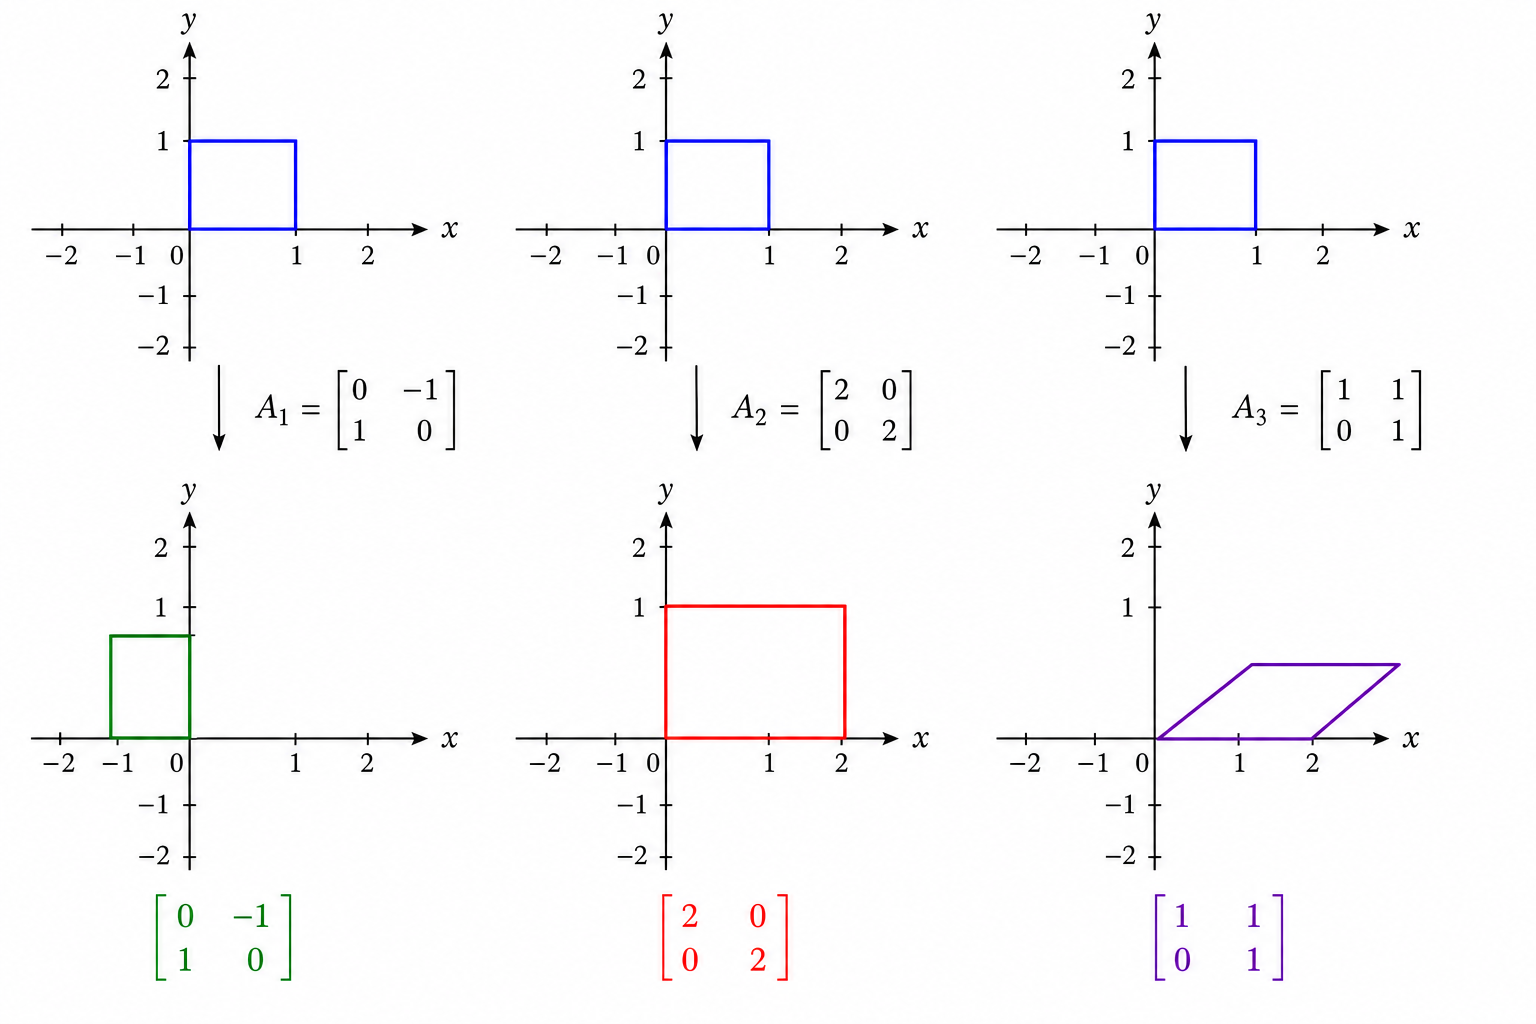
\includegraphics[width=0.62\textwidth]{Figures/png_ready/34-matrix-transformation-manual.png}
    \caption{แผนภาพแสดงการหมุน การขยาย และการเฉือนด้วยเมทริกซ์}
    \label{fig:matrix-transformation}
\end{figure}

เมทริกซ์ใช้ในการแปลงภาพกราฟิก 2 มิติ และ 3 มิติ อย่างมีประสิทธิภาพ โดยการแปลงหลักๆ ประกอบด้วยการเลื่อน (translation) การขยายหรือหด (scaling) และการหมุน (rotation) ซึ่งสามารถเขียนในรูปเมทริกซ์ได้โดยใช้ homogeneous coordinates ซึ่งเป็นเทคนิคที่เพิ่มมิติให้กับจุดเพื่อให้การแปลงทุกรูปแบบสามารถเขียนในรูปการคูณเมทริกซ์ได้อย่างเป็นหนึ่งเดียว หลักการนี้ถูกนำไปใช้ในโปรแกรมกราฟิกทุกประเภทตั้งแต่การวาดรูปง่ายๆ ไปจนถึงเกม 3 มิติขั้นสูง

\begin{ex}[การแปลง 2 มิติ]
การแปลงจุด $(x, y)$ ในระบบ 2 มิติ สามารถเขียนในรูปเมทริกซ์ได้ดังนี้

\[
\begin{pmatrix} x' \\ y' \\ 1 \end{pmatrix} = T \begin{pmatrix} x \\ y \\ 1 \end{pmatrix}
\]

โดยใช้ homogeneous coordinates
\end{ex}
\begin{solution}
\begin{align*}
\text{เลื่อน:}\quad T &= \begin{pmatrix} 1 & 0 & t_x \\ 0 & 1 & t_y \\ 0 & 0 & 1 \end{pmatrix}, &
\text{ขยาย:}\quad S &= \begin{pmatrix} s_x & 0 & 0 \\ 0 & s_y & 0 \\ 0 & 0 & 1 \end{pmatrix}\\
\text{หมุน:}\quad R &= \begin{pmatrix} \cos\theta & -\sin\theta & 0 \\ \sin\theta & \cos\theta & 0 \\ 0 & 0 & 1 \end{pmatrix}
\end{align*}
การแปลงผสม: $P' = T\cdot R\cdot S\cdot P$ \solhere
\end{solution}

\begin{ex}
หมุนจุด $(1, 0)$ รอบจุดกำเนิด $90^\circ$ โดยใช้เมทริกซ์การหมุน $R = \begin{pmatrix} 0 & -1 & 0 \\ 1 & 0 & 0 \\ 0 & 0 & 1 \end{pmatrix}$
\end{ex}
\begin{solution}
\[
P' = RP = \begin{pmatrix} 0 & -1 & 0 \\ 1 & 0 & 0 \\ 0 & 0 & 1 \end{pmatrix}\begin{pmatrix} 1 \\ 0 \\ 1 \end{pmatrix} = \begin{pmatrix} 0 \\ 1 \\ 1 \end{pmatrix}
\]
$\therefore$ จุดใหม่คือ $(0,1)$ \solhere
\end{solution}

\subsection{การเข้ารหัส Hill Cipher}
Hill Cipher เป็นระบบเข้ารหัสแบบบล็อกที่พัฒนาโดย Lester Hill ในปี ค.ศ. 1929 โดยใช้ความรู้เรื่องเมทริกซ์เป็นพื้นฐาน ข้อความธรรมดาถูกแปลงเป็นเวกเตอร์ตัวเลข แล้วคูณด้วยเมทริกซ์กุญแจ $K$ ผลลัพธ์คือข้อความเข้ารหัส ความแข็งแกร่งของ Hill Cipher อยู่ที่การกระจายตัวอักษรแต่ละตัวไปยังหลายตำแหน่งในข้อความเข้ารหัส ทำให้การวิเคราะห์ความถี่ตัวอักษร (frequency analysis) ไม่สามารถถอดรหัสได้โดยตรง

\begin{ex}
กำหนดเมทริกซ์กุญแจ $K = \begin{pmatrix} 3 & 2 \\ 1 & 1 \end{pmatrix}$ เข้ารหัสข้อความ ``HI''
\end{ex}
\begin{solution}
กำหนด A$=0$, \ldots, Z$=25$ จึงได้ H$=7$, I$=8$
\begin{align*}
P &= \begin{pmatrix} 7 \\ 8 \end{pmatrix}\\
C = KP &= \begin{pmatrix} 3 & 2 \\ 1 & 1 \end{pmatrix}\begin{pmatrix} 7 \\ 8 \end{pmatrix} = \begin{pmatrix} 37 \\ 15 \end{pmatrix} \equiv \begin{pmatrix} 11 \\ 15 \end{pmatrix} \pmod{26}
\end{align*}
$11=$L, $15=$P $\therefore$ ``HI'' $\to$ ``LP'' \solhere
\end{solution}

หมายเหตุ: การถอดรหัสต้องใช้ $K^{-1}$ ซึ่งมีอยู่ก็ต่อเมื่อ $\det(K) \neq 0 \pmod{26}$ นั่นคือ $\gcd(\det(K), 26) = 1$ ในกรณีนี้ $\det(K) = 3(1) - 2(1) = 1$ และ $\gcd(1, 26) = 1$ ดังนั้นตัวผกผันมีอยู่

\begin{ex}
ถอดรหัส ``LP'' กลับเป็น ``HI'' โดยใช้เมทริกซ์กุญแจ $K = \begin{pmatrix} 3 & 2 \\ 1 & 1 \end{pmatrix}$
\end{ex}
\begin{solution}
\begin{align*}
K^{-1} &= \begin{pmatrix} 1 & -2 \\ -1 & 3 \end{pmatrix} \pmod{26} \quad (\det K = 1)\\
P = K^{-1}C &= \begin{pmatrix} 1 & -2 \\ -1 & 3 \end{pmatrix}\begin{pmatrix} 11 \\ 15 \end{pmatrix} = \begin{pmatrix} -19 \\ 34 \end{pmatrix} \equiv \begin{pmatrix} 7 \\ 8 \end{pmatrix} \pmod{26}
\end{align*}
$7=$H, $8=$I $\therefore$ ได้ข้อความเดิม ``HI'' \solhere
\end{solution}

\subsection{เมทริกซ์ประชิดในทฤษฎีกราฟ}
เมทริกซ์ประชิดเป็นเครื่องมือสำคัญในการแทนกราฟในรูปแบบเมทริกซ์ ทำให้สามารถใช้คุณสมบัติทางพีชคณิตในการวิเคราะห์กราฟได้

\begin{ex}
Adjacency Matrix ของกราฟ $G$ ที่มี $n$ โหนด คือเมทริกซ์ $A$ ขนาด $n \times n$ โดยที่ $a_{ij} = 1$ ถ้ามีเส้นเชื่อมระหว่างโหนด $i$ และ $j$ และ $a_{ij} = 0$ ในกรณีอื่น โดยสมบัติที่สำคัญคือ $(A^k)_{ij}$ บอกจำนวนเส้นทางความยาว $k$ จากโหนด $i$ ไปยังโหนด $j$ และผลรวมของแถวที่ $i$ เท่ากับ degree ของโหนด $i$
\end{ex}
\begin{solution}
สร้าง $A_{n\times n}$ โดย $a_{ij}=1$ ถ้ามีเส้นเชื่อม $i$–$j$ มิฉะนั้น $0$; สมบัติ: $(A^k)_{ij}=$ จำนวนเส้นทางยาว $k$ จาก $i$ ไป $j$, และผลรวมแถว $i$ $=$ degree ของโหนด $i$ \solhere
\end{solution}

\begin{ex}
พิจารณากราฟรูปสามเหลี่ยม (3 โหนด เชื่อมกันทุกคู่) เมทริกซ์ประชิด (adjacency matrix) $A$ และกำลังสองของมันคือ
\[
A = \begin{pmatrix} 0 & 1 & 1 \\ 1 & 0 & 1 \\ 1 & 1 & 0 \end{pmatrix},
\qquad
A^2 = \begin{pmatrix} 2 & 1 & 1 \\ 1 & 2 & 1 \\ 1 & 1 & 2 \end{pmatrix}.
\]
สมาชิก $(A^2)_{ij}$ บอกจำนวนเส้นทาง 2 ขั้นจากโหนด $i$ ไปโหนด $j$ เช่น $(A^2)_{12} = 1$ หมายความว่ามี 1 เส้นทาง 2 ขั้นจากโหนด 1 ไปโหนด 2 (คือ $1 \to 3 \to 2$)
\end{ex}
\begin{solution}
\[
A = \begin{pmatrix} 0 & 1 & 1 \\ 1 & 0 & 1 \\ 1 & 1 & 0 \end{pmatrix} \Rightarrow A^2 = \begin{pmatrix} 2 & 1 & 1 \\ 1 & 2 & 1 \\ 1 & 1 & 2 \end{pmatrix}
\]
$(A^2)_{12}=1$: มี 1 เส้นทาง 2 ขั้น $1\to 3\to 2$; แนวทแยง $=2$ (แต่ละโหนดมี 2 เส้นทางกลับตัวเองผ่านโหนดอื่น) \solhere
\end{solution}

\subsection{เมทริกซ์ในการเรียนรู้ของเครื่อง}
ในการเรียนรู้ของเครื่อง (Machine Learning) ข้อมูลและพารามิเตอร์ของโมเดลมักถูกจัดเก็บในรูปเมทริกซ์ ทำให้การคำนวณจำนวนมหาศาลสรุปลงเหลือเพียงการคูณเมทริกซ์ไม่กี่ครั้ง ในที่นี้ยกตัวอย่างพื้นฐานสองแบบ คือ การถดถอยเชิงเส้น (Linear Regression) และโครงข่ายประสาทเทียม (Neural Network)

\begin{ex}[การถดถอยเชิงเส้น]
โมเดล Linear Regression เขียนในรูปเมทริกซ์เป็น $y = X\beta$ โดย $X$ คือเมทริกซ์ข้อมูล (design matrix) และ $\beta$ คือเวกเตอร์สัมประสิทธิ์ ค่าที่เหมาะที่สุดหาได้จาก normal equation $\beta = (X^T X)^{-1} X^T y$ จงหา $\beta$ สำหรับข้อมูล
\[
X = \begin{pmatrix} 1 & 2 \\ 1 & 4 \\ 1 & 6 \end{pmatrix}, \qquad
y = \begin{pmatrix} 3 \\ 5 \\ 7 \end{pmatrix}
\]
\end{ex}
\begin{solution}
\begin{align*}
X^T X &= \begin{pmatrix} 3 & 12 \\ 12 & 56 \end{pmatrix}, \quad \det = 24 \neq 0\\
(X^T X)^{-1} &= \tfrac{1}{24}\begin{pmatrix} 56 & -12 \\ -12 & 3 \end{pmatrix}, \quad X^T y = \begin{pmatrix} 15 \\ 68 \end{pmatrix}\\
\beta = (X^T X)^{-1} X^T y &= \begin{pmatrix} 1 \\ 1 \end{pmatrix}
\end{align*}
$\therefore y = 1 + x$ \solhere
\end{solution}

\begin{ex}[โครงข่ายประสาทเทียมหนึ่งชั้น]
โครงข่ายประสาทเทียมหนึ่งชั้น (single-layer neural network) คำนวณผลลัพธ์จาก $\mathbf{z} = \mathbf{x} W + \mathbf{b}$ แล้วส่งผ่านฟังก์ชันกระตุ้น (activation function) ReLU $f(z) = \max(0, z)$ จงหาผลลัพธ์ของชั้นนี้เมื่อ
\[
\mathbf{x} = \begin{pmatrix} 1 & 0.5 \end{pmatrix}, \qquad
W = \begin{pmatrix} 0.8 & 0.2 \\ 0.3 & 0.7 \end{pmatrix}, \qquad
\mathbf{b} = \begin{pmatrix} -0.5 & 0.1 \end{pmatrix}
\]
\end{ex}
\begin{solution}
\begin{align*}
\mathbf{z} &= \mathbf{x} W + \mathbf{b} = \begin{pmatrix} 1 & 0.5 \end{pmatrix}\begin{pmatrix} 0.8 & 0.2 \\ 0.3 & 0.7 \end{pmatrix} + \begin{pmatrix} -0.5 & 0.1 \end{pmatrix}\\
&= \begin{pmatrix} 0.95 & 0.55 \end{pmatrix} + \begin{pmatrix} -0.5 & 0.1 \end{pmatrix} = \begin{pmatrix} 0.45 & 0.65 \end{pmatrix}\\
f(\mathbf{z}) &= \mathrm{ReLU}(\mathbf{z}) = \begin{pmatrix} 0.45 & 0.65 \end{pmatrix}
\end{align*}
\solhere
\end{solution}

\sectionbanner{สรุปบทเรียน}
บทนี้ศึกษาเมทริกซ์และดีเทอร์มิแนนต์ซึ่งเป็นเครื่องมือพื้นฐานในคณิตศาสตร์และวิทยาการคอมพิวเตอร์ เริ่มจากเมทริกซ์ซึ่งเป็นการจัดเรียงข้อมูลในรูปตารางสองมิติและมีหลายประเภท เช่น เมทริกซ์จตุรัส เส้นทแยงมุม สมมาตร และสามเหลี่ยม ต่อด้วยการดำเนินการระหว่างเมทริกซ์ ได้แก่ การบวก ลบ คูณด้วยสเกลาร์ คูณเมทริกซ์ และการสลับเปลี่ยน (transpose) โดยการคูณเมทริกซ์ไม่มีสมบัติการสลับที่ ดีเทอร์มิแนนต์เป็นค่าจำเพาะของเมทริกซ์จตุรัสที่คำนวณได้ด้วยการกระจายโคแฟกเตอร์ (cofactor expansion) หรือกฎของ Sarrus สำหรับเมทริกซ์ $3 \times 3$ และมีสมบัติสำคัญคือ $\det(AB) = \det(A)\det(B)$ ตัวผกผัน $A^{-1}$ ทำให้ $AA^{-1} = A^{-1}A = I$ และมีได้ก็ต่อเมื่อ $\det(A) \neq 0$ ระบบสมการเชิงเส้นแก้ได้ด้วยตัวผกผันเมทริกซ์ ($x = A^{-1}b$) กฎของคราเมอร์ หรือการกำจัดแบบเกาส์ (Gaussian elimination) และนำไปประยุกต์ในคอมพิวเตอร์กราฟิกส์ การเข้ารหัส การเรียนรู้ของเครื่อง และทฤษฎีกราฟ

เมทริกซ์เป็นพื้นฐานที่จำเป็นสำหรับการศึกษาต่อในสาขาคณิตศาสตร์ขั้นสูง เช่น พีชคณิตเชิงเส้น (Linear Algebra) และการวิเคราะห์เชิงตัวเลข (Numerical Analysis)~\cite{strang2023linear}

\clearpage
\sectionbanner{แบบฝึกหัด}
\exercisepart{ส่วนที่ 1: พื้นฐานเมทริกซ์}
\begin{exercise}
จงระบุขนาดของเมทริกซ์ต่อไปนี้
\begin{enumerate}
    \item $A = \begin{pmatrix} 1 & 2 & 3 \\ 4 & 5 & 6 \end{pmatrix}$
    \item $B = \begin{pmatrix} 1 & 0 \\ 0 & 1 \\ 1 & 0 \end{pmatrix}$
    \item $C = \begin{pmatrix} 3 \end{pmatrix}$
\end{enumerate}
\end{exercise}

\begin{exercise}
จงระบุว่าเมทริกซ์ต่อไปนี้เป็นเมทริกซ์ชนิดใด (จตุรัส, สมมาตร, สามเหลี่ยมบน, สามเหลี่ยมล่าง, เส้นทแยงมุม, เอกลักษณ์, ศูนย์)
\begin{enumerate}
    \item $A = \begin{pmatrix} 1 & 0 & 0 \\ 0 & 2 & 0 \\ 0 & 0 & 3 \end{pmatrix}$
    \item $B = \begin{pmatrix} 1 & 2 \\ 2 & 1 \end{pmatrix}$
    \item $C = \begin{pmatrix} 1 & 1 & 1 \\ 0 & 1 & 1 \\ 0 & 0 & 1 \end{pmatrix}$
\end{enumerate}
\end{exercise}

\exercisepart{ส่วนที่ 2: การดำเนินการระหว่างเมทริกซ์}
\begin{exercise}
กำหนด $A = \begin{pmatrix} 1 & 2 \\ 3 & 4 \end{pmatrix}$ และ $B = \begin{pmatrix} 5 & 6 \\ 7 & 8 \end{pmatrix}$ จงหา
\begin{enumerate}
    \item $A + B$
    \item $A - B$
    \item $3A$
    \item $A \cdot B$
    \item $B \cdot A$
\end{enumerate}
\end{exercise}

\begin{exercise}
จงหา transpose ของเมทริกซ์ต่อไปนี้
\begin{enumerate}
    \item $A = \begin{pmatrix} 1 & 2 & 3 \\ 4 & 5 & 6 \end{pmatrix}$
    \item $B = \begin{pmatrix} 1 & 2 \\ 3 & 4 \\ 5 & 6 \end{pmatrix}$
\end{enumerate}
\end{exercise}

\exercisepart{ส่วนที่ 3: ดีเทอร์มิแนนต์}
\begin{exercise}
จงคำนวณดีเทอร์มิแนนต์ของเมทริกซ์ต่อไปนี้โดยใช้วิธี cofactor expansion:
\begin{enumerate}
    \item $\det\begin{pmatrix} 1 & 2 \\ 3 & 4 \end{pmatrix}$
    \item $\det\begin{pmatrix} 1 & 0 & 2 \\ 3 & 1 & 4 \\ 5 & 6 & 1 \end{pmatrix}$
\end{enumerate}
\end{exercise}

\begin{exercise}
จงคำนวณดีเทอร์มิแนนต์โดยใช้กฎของ Sarrus:
\begin{enumerate}
    \item $\det\begin{pmatrix} 1 & 2 & 3 \\ 4 & 5 & 6 \\ 7 & 8 & 9 \end{pmatrix}$
\end{enumerate}
\end{exercise}

\exercisepart{ส่วนที่ 4: ตัวผกผันของเมทริกซ์}
\begin{exercise}
จงหาตัวผกผันของเมทริกซ์ต่อไปนี้ (ถ้ามี)
\begin{enumerate}
    \item $A = \begin{pmatrix} 1 & 2 \\ 3 & 4 \end{pmatrix}$
    \item $B = \begin{pmatrix} 2 & 1 \\ 4 & 2 \end{pmatrix}$
    \item $I = \begin{pmatrix} 1 & 0 & 0 \\ 0 & 1 & 0 \\ 0 & 0 & 1 \end{pmatrix}$
\end{enumerate}
\end{exercise}

\begin{exercise}
จงตรวจสอบว่า $A \cdot A^{-1} = A^{-1} \cdot A = I$ สำหรับข้อ 1(a)
\end{exercise}

\exercisepart{ส่วนที่ 5: การแก้ระบบสมการเชิงเส้น}
\begin{exercise}
จงแก้ระบบสมการต่อไปนี้โดยใช้ตัวผกผันเมทริกซ์
\begin{enumerate}
    \item $x + 2y = 5,\ 3x + 4y = 6$
    \item $2x + y = 3,\ x - y = 1$
\end{enumerate}
\end{exercise}

\begin{exercise}
จงแก้ระบบสมการต่อไปนี้โดยใช้กฎของคราเมอร์
\begin{enumerate}
    \item $x + y = 2,\ 2x + 3y = 5$
\end{enumerate}
\end{exercise}

\clearpage
\answerkeyhead
เฉลยอย่างย่อสำหรับแบบฝึกหัดในแต่ละส่วน เพื่อให้ผู้เรียนใช้ตรวจคำตอบของตนเอง

\exercisepart{ส่วนที่ 1: พื้นฐานเมทริกซ์}
\begin{enumerate}[label={},leftmargin=0pt]
    \item ขนาด
    \begin{enumerate}[label=\textbf{\thechapter.\arabic{enumi}.\arabic*}]
        \item $2\times 3$
        \item $3\times 2$
        \item $1\times 1$
    \end{enumerate}

    \item ประเภท
    \begin{enumerate}[label=\textbf{\thechapter.\arabic{enumi}.\arabic*}]
        \item จตุรัส เส้นทแยงมุม (และเป็นสมมาตร สามเหลี่ยมบน สามเหลี่ยมล่างพร้อมกัน)
        \item จตุรัส สมมาตร
        \item จตุรัส สามเหลี่ยมบน
    \end{enumerate}
\end{enumerate}

\exercisepart{ส่วนที่ 2: การดำเนินการระหว่างเมทริกซ์}
\begin{enumerate}[label={},leftmargin=0pt,start=3]
    \item การดำเนินการ
    \begin{enumerate}[label=\textbf{\thechapter.\arabic{enumi}.\arabic*}]
        \item $A+B = \begin{pmatrix}6 & 8\\ 10 & 12\end{pmatrix}$
        \item $A-B = \begin{pmatrix}-4 & -4\\ -4 & -4\end{pmatrix}$
        \item $3A = \begin{pmatrix}3 & 6\\ 9 & 12\end{pmatrix}$
        \item $AB = \begin{pmatrix}19 & 22\\ 43 & 50\end{pmatrix}$
        \item $BA = \begin{pmatrix}23 & 34\\ 31 & 46\end{pmatrix}$ (ยืนยันว่า $AB\neq BA$)
    \end{enumerate}

    \item เมทริกซ์สลับเปลี่ยน
    \begin{enumerate}[label=\textbf{\thechapter.\arabic{enumi}.\arabic*}]
        \item $A^T = \begin{pmatrix}1 & 4\\ 2 & 5\\ 3 & 6\end{pmatrix}$
        \item $B^T = \begin{pmatrix}1 & 3 & 5\\ 2 & 4 & 6\end{pmatrix}$
    \end{enumerate}
\end{enumerate}

\exercisepart{ส่วนที่ 3: ดีเทอร์มิแนนต์}
\begin{enumerate}[label={},leftmargin=0pt,start=5]
    \item ดีเทอร์มิแนนต์
    \begin{enumerate}[label=\textbf{\thechapter.\arabic{enumi}.\arabic*}]
        \item $\det = (1)(4)-(2)(3) = -2$
        \item กระจายตามแถวที่ 1: $1\cdot(1-24) - 0 + 2\cdot(18-5) = -23 + 26 = 3$
    \end{enumerate}
    \item Sarrus: $aei+bfg+cdh-ceg-bdi-afh = 45+84+96-105-72-48 = 0$
\end{enumerate}

\exercisepart{ส่วนที่ 4: ตัวผกผันของเมทริกซ์}
\begin{enumerate}[label={},leftmargin=0pt,start=7]
    \item การหาตัวผกผัน
    \begin{enumerate}[label=\textbf{\thechapter.\arabic{enumi}.\arabic*}]
        \item $\det(A) = -2 \neq 0$, $A^{-1} = -\frac{1}{2}\begin{pmatrix}4 & -2\\ -3 & 1\end{pmatrix} = \begin{pmatrix}-2 & 1\\ \frac{3}{2} & -\frac{1}{2}\end{pmatrix}$
        \item $\det(B) = 0$ จึงไม่มีตัวผกผัน
        \item $I^{-1} = I$
    \end{enumerate}
    \item $A\cdot A^{-1} = \begin{pmatrix}1 & 2\\ 3 & 4\end{pmatrix}\begin{pmatrix}-2 & 1\\ \frac{3}{2} & -\frac{1}{2}\end{pmatrix} = \begin{pmatrix}1 & 0\\ 0 & 1\end{pmatrix} = I$ และตรวจ $A^{-1}\cdot A = I$ เช่นกัน
\end{enumerate}

\exercisepart{ส่วนที่ 5: การแก้ระบบสมการเชิงเส้น}
\begin{enumerate}[label={},leftmargin=0pt,start=9]
    \item การแก้ระบบสมการด้วยตัวผกผัน
    \begin{enumerate}[label=\textbf{\thechapter.\arabic{enumi}.\arabic*}]
        \item $A^{-1}b = \begin{pmatrix}-2 & 1\\ \frac{3}{2} & -\frac{1}{2}\end{pmatrix}\begin{pmatrix}5\\ 6\end{pmatrix} = \begin{pmatrix}-4\\ \frac{9}{2}\end{pmatrix}$ ดังนั้น $x=-4, y=\frac{9}{2}$
        \item $\det(A) = -3$, $A^{-1} = -\frac{1}{3}\begin{pmatrix}-1 & -1\\ -1 & 2\end{pmatrix} = \begin{pmatrix}\frac{1}{3} & \frac{1}{3}\\ \frac{1}{3} & -\frac{2}{3}\end{pmatrix}$ ดังนั้น $\begin{pmatrix}x\\y\end{pmatrix} = A^{-1}b = \begin{pmatrix}\frac{1}{3} & \frac{1}{3}\\ \frac{1}{3} & -\frac{2}{3}\end{pmatrix}\begin{pmatrix}3\\1\end{pmatrix} = \begin{pmatrix}\frac{4}{3}\\ \frac{1}{3}\end{pmatrix}$
    \end{enumerate}
    \item กฎคราเมอร์ $\det A = 1$, $\det A_x = \begin{vmatrix}2 & 1\\ 5 & 3\end{vmatrix} = 1$, $\det A_y = \begin{vmatrix}1 & 2\\ 2 & 5\end{vmatrix} = 1$ ดังนั้น $x = 1, y = 1$
\end{enumerate}

\newpage
\QAChapter
\begin{enumerate}
    \item จงระบุขนาดของเมทริกซ์ต่อไปนี้ และระบุจำนวนสมาชิกทั้งหมด
    \begin{enumerate}
        \item $A = \begin{pmatrix} 1 & 2 & 3 \\ 4 & 5 & 6 \end{pmatrix}$
        \item $B = \begin{pmatrix} 1 & 0 \\ 0 & 1 \\ 1 & 0 \end{pmatrix}$
        \item $C = \begin{pmatrix} 3 \end{pmatrix}$
    \end{enumerate}
    \item จงบอกประเภทของเมทริกซ์ต่อไปนี้ (จตุรัส, สมมาตร, สามเหลี่ยมบน, สามเหลี่ยมล่าง, เส้นทแยงมุม, เอกลักษณ์, ศูนย์)
    \begin{enumerate}
        \item $A = \begin{pmatrix} 1 & 0 & 0 \\ 0 & 2 & 0 \\ 0 & 0 & 3 \end{pmatrix}$
        \item $B = \begin{pmatrix} 1 & 2 \\ 2 & 1 \end{pmatrix}$
        \item $C = \begin{pmatrix} 1 & 1 & 1 \\ 0 & 1 & 1 \\ 0 & 0 & 1 \end{pmatrix}$
    \end{enumerate}
    \item กำหนด $A = \begin{pmatrix} 1 & 2 \\ 3 & 4 \end{pmatrix}$ และ $B = \begin{pmatrix} 5 & 6 \\ 7 & 8 \end{pmatrix}$ จงหา $A + B$, $A - B$, $3A$, $A \cdot B$, และ $B \cdot A$
    \item จงพิสูจน์ว่า $(AB)^T = B^T A^T$ สำหรับเมทริกซ์ $A$ และ $B$ ขนาด $2 \times 2$
    \item จงคำนวณดีเทอร์มิแนนต์ของเมทริกซ์ต่อไปนี้โดยวิธี cofactor expansion:
    \begin{enumerate}
        \item $\det\begin{pmatrix} 1 & 2 \\ 3 & 4 \end{pmatrix}$
        \item $\det\begin{pmatrix} 1 & 0 & 2 \\ 3 & 1 & 4 \\ 5 & 6 & 1 \end{pmatrix}$
    \end{enumerate}
    \item จงหาตัวผกผันของ $A = \begin{pmatrix} 2 & 1 \\ 1 & 1 \end{pmatrix}$ (ถ้ามี) และตรวจสอบ $A \cdot A^{-1} = I$
    \item จงแก้ระบบสมการ $x + 2y = 5,\ 3x + 4y = 11$ โดยใช้ตัวผกผันเมทริกซ์
    \item จงอธิบายการประยุกต์ใช้เมทริกซ์ในงานด้านคอมพิวเตอร์กราฟิกส์ พร้อมยกตัวอย่างการแปลงเมทริกซ์
\end{enumerate}

\newpage
\sheetChapter{เมทริกซ์และดีเทอร์มิแนนต์ (Matrices \& Determinants)}
\section*{วัตถุประสงค์}
\begin{enumerate}
    \item เพื่อให้ผู้เรียนเข้าใจนิยามและประเภทของเมทริกซ์
    \item เพื่อให้ผู้เรียนสามารถดำเนินการบวก ลบ คูณเมทริกซ์ได้
    \item เพื่อให้ผู้เรียนคำนวณดีเทอร์มิแนนต์และหาตัวผกผันได้
    \item เพื่อให้ผู้เรียนประยุกต์ใช้เมทริกซ์ในการแก้ระบบสมการเชิงเส้น
\end{enumerate}
\section*{คำชี้แจง} ให้ผู้เรียนศึกษาเนื้อหาบทเมทริกซ์และดีเทอร์มิแนนต์ แล้วตอบคำถามต่อไปนี้
\begin{enumerate}
    \item ให้ผู้เรียนอธิบายความหมายของเมทริกซ์ พร้อมยกตัวอย่างเมทริกซ์ขนาด $3 \times 2$
    \Pointilles{3}
    \item ให้ผู้เรียนยกตัวอย่างเมทริกซ์ประเภทต่างๆ ที่กล่าวในบทเรียน
    \Pointilles{3}
    \item ให้ผู้เรียนอธิบายขั้นตอนการคูณเมทริกซ์ $A_{m \times n} \cdot B_{n \times p}$ พร้อมยกตัวอย่าง
    \Pointilles{3}
    \item ให้ผู้เรียนสรุปสมบัติของดีเทอร์มิแนนต์ที่สำคัญ
    \Pointilles{3}
    \item ให้ผู้เรียนอธิบายเงื่อนไขที่เมทริกซ์จะมีตัวผกผัน พร้อมยกตัวอย่าง
    \Pointilles{3}
    \item ให้ผู้เรียนอธิบายการประยุกต์ใช้เมทริกซ์ในงานด้านวิทยาการคอมพิวเตอร์อย่างน้อย 2 ตัวอย่าง
    \Pointilles{3}
\end{enumerate}

	\RefChapter
	
	%% บทที่ 6
	\cleartoleftpage
	\introChapter{พีชคณิตบูลีน (Boolean Algebra)}

\begin{description}[leftmargin=2.5cm, style=nextline]
    \item[รหัสวิชา] 4091606
    \item[ชื่อวิชา] คณิตศาสตร์สำหรับคอมพิวเตอร์
    \item[หน่วยกิต] 3 (3-0-6)
    \item[บทที่] 6
    \item[ชื่อบท] พีชคณิตบูลีน (Boolean Algebra)
    \item[จำนวนชั่วโมง] 9 ชั่วโมง
\end{description}

\vspace{1em}
\noindent วัตถุประสงค์การเรียนรู้ประจำบท\\[0.3em]
\noindent เมื่อนักศึกษาเรียนบทนี้จบแล้ว นักศึกษาจะสามารถ
\begin{enumerate}[topsep=0.3em, itemsep=0.25em]
    \item อธิบายสัจพจน์และกฎของพีชคณิตบูลีนได้
    \item ลดรูปสมการบูลีนโดยใช้กฎพีชคณิตบูลีนได้
    \item สร้างและวิเคราะห์วงจรประตูตรรกะจากนิพจน์บูลีนได้
    \item ใช้แผนที่การ์โนในการลดรูปฟังก์ชันบูลีนได้
    \item เชื่อมโยงพีชคณิตบูลีนกับการออกแบบวงจรดิจิทัลและการเขียนโปรแกรมได้
\end{enumerate}

\vspace{1em}
\noindent หัวข้อที่สอน\\[0.3em]
\begin{enumerate}[topsep=0.3em, itemsep=0.25em]
    \item สัจพจน์และกฎของพีชคณิตบูลีน
    \item การลดรูปนิพจน์บูลีน
    \item วงจรประตูตรรกะ
    \item แผนที่การ์โน
    \item การประยุกต์ใช้พีชคณิตบูลีนในวงจรดิจิทัล
\end{enumerate}

\vspace{1em}
\noindent สื่อการสอน
\begin{enumerate}[topsep=0.3em, itemsep=0.25em]
    \item สไลด์ประกอบการสอน
    \item ซอฟต์แวร์จำลองวงจรลอจิก
    \item แบบฝึกหัดท้ายบท
\end{enumerate}

	\cleartoleftpage
	\chapter{พีชคณิตบูลีน (Boolean Algebra)}
\label{ch:boolean}

พีชคณิตบูลีน (Boolean Algebra) เป็นระบบคณิตศาสตร์ที่ศึกษาเกี่ยวกับค่าทางตรรกศาสตร์ 2 สถานะ ได้แก่ 0 (เท็จ) และ 1 (จริง) รวมถึงการดำเนินการทางตรรกะพื้นฐาน โดยพีชคณิตบูลีนทำหน้าที่เป็นรากฐานสำคัญในการออกแบบวงจรดิจิทัล การสร้างเงื่อนไขควบคุมในโปรแกรมคอมพิวเตอร์ และการสืบค้นข้อมูลในระบบฐานข้อมูล~\parencite{mano2018digital}

พีชคณิตบูลีนมีความเชื่อมโยงโดยตรงกับทฤษฎีเซตและตรรกศาสตร์ประพจน์ โดยค่า 0 สอดคล้องกับเซตว่าง ($\emptyset$) ในทฤษฎีเซตและประพจน์ที่เป็นเท็จ ($\bot$) ในตรรกศาสตร์ ในขณะที่ค่า 1 สอดคล้องกับเอกภพสัมพัทธ์ ($U$) และประพจน์ที่เป็นจริง ($\top$) ดังแสดงการเปรียบเทียบในตารางที่~\ref{tab:boolean-set-logic}

เมื่อกำหนดเอกภพสัมพัทธ์ $U$ และเซตย่อย $A, B \subseteq U$ จะพบว่าการดำเนินการ OR สอดคล้องกับยูเนียน ($A \cup B$), การดำเนินการ AND สอดคล้องกับอินเตอร์เซกชัน ($A \cap B$) และการดำเนินการ NOT สอดคล้องกับคอมพลีเมนต์ ($A^c = U - A$) ความสอดคล้องกันนี้ช่วยให้ผู้เรียนสามารถประยุกต์ใช้แนวคิดและกฎทางคณิตศาสตร์ชุดเดียวกันในการทำความเข้าใจทั้งตรรกศาสตร์ ทฤษฎีเซต และการทำงานของวงจรดิจิทัล

\begin{table}[!htb]
    \centering
    \caption{ความสัมพันธ์ระหว่างพีชคณิตบูลีน ทฤษฎีเซต และตรรกศาสตร์}
    \label{tab:boolean-set-logic}
    \begin{tabular}{|c|c|c|}
        \hline
        พีชคณิตบูลีน & ทฤษฎีเซต & ตรรกศาสตร์ประพจน์ \\
        \hline
        0 (เท็จ) & $\emptyset$ (เซตว่าง) & $\bot$ (เท็จ) \\
        \hline
        1 (จริง) & $U$ (เอกภพสัมพัทธ์) & $\top$ (จริง) \\
        \hline
        การดำเนินการ OR ($+$) & ยูเนียน ($\cup$) & การดำเนินการ OR ($\lor$) \\
        \hline
        การดำเนินการ AND ($\cdot$) & อินเตอร์เซกชัน ($\cap$) & การดำเนินการ AND ($\land$) \\
        \hline
        การดำเนินการ NOT ($\overline{x}$) & คอมพลีเมนต์ ($A^c$) & การดำเนินการ NOT ($\neg$) \\
        \hline
    \end{tabular}
\end{table}

\section{นิยามพื้นฐานของพีชคณิตบูลีน}
\label{sec:boolean-definitions}

พีชคณิตบูลีนประกอบด้วยองค์ประกอบหลัก 3 ส่วน ได้แก่ เซตของค่าคงตัวที่ตัวแปรสามารถรับค่าได้ ตัวดำเนินการที่กระทำกับค่าเหล่านั้น และสัจพจน์หรือกฎพื้นฐานที่กำกับการดำเนินการ หัวข้อนี้จะนำเสนอโครงสร้างเชิงพีชคณิตบูลีนอย่างเป็นทางการ พร้อมทั้งอธิบายความหมายของค่าคงตัวทั้งสองค่า เพื่อเป็นพื้นฐานในการศึกษาหัวข้อถัดไปตลอดทั้งบทเรียน~\parencite{mano2018digital}

\subsection{นิยามของพีชคณิตบูลีน}
พีชคณิตบูลีนเป็นโครงสร้างเชิงพีชคณิตที่กำหนดขึ้นเพื่ออธิบายกระบวนการให้เหตุผลเชิงตรรกะและการทำงานของระบบดิจิทัล โดยประกอบด้วยค่าพื้นฐานเพียง 2 ค่าและการดำเนินการตรรกะ พร้อมทั้งสัจพจน์ (Axioms) ที่ควบคุมการดำเนินการเหล่านั้น ข้อแตกต่างสำคัญระหว่างพีชคณิตบูลีนกับพีชคณิตของจำนวนจริง คือ ตัวแปรในพีชคณิตบูลีนสามารถมีค่าได้เพียงสองสถานะเท่านั้น และไม่มีการดำเนินการผกผัน เช่น การลบหรือการหาร ส่งผลให้กฎทางพีชคณิตบางข้อที่ไม่เป็นจริงในระบบจำนวนจริง สามารถเป็นจริงได้ในพีชคณิตบูลีน เช่น กฎการบวกซ้ำ $a + a = a$~\parencite{mano2018digital}

\begin{definition}[พีชคณิตบูลีน]
\index{พีชคณิตบูลีน!นิยาม}
พีชคณิตบูลีน คือ โครงสร้างเชิงพีชคณิต $(B, +, \cdot, ', 0, 1)$ โดยที่ $B$ เป็นเซตที่มีสองสมาชิกคือ $\{0, 1\}$ พร้อมการดำเนินการทวิภาค $+$ และ $\cdot$ และการดำเนินการเอกภาค $'$ โดยสอดคล้องกับสัจพจน์ต่อไปนี้

\begin{enumerate}
    \item กฎการปิด (Closure Laws) สำหรับทุก $a, b \in B$ ได้ว่า
    \begin{enumerate}
        \item $a + b \in B$
        \item $a \cdot b \in B$
    \end{enumerate}
    \item กฎการมีเอกลักษณ์ (Identity Elements)
    \begin{enumerate}
        \item $a + 0 = a$ ($0$ เป็นเอกลักษณ์ของ OR)
        \item $a \cdot 1 = a$ ($1$ เป็นเอกลักษณ์ของ AND)
    \end{enumerate}
    \item กฎการสลับที่ (Commutative Laws)
    \begin{enumerate}
        \item $a + b = b + a$
        \item $a \cdot b = b \cdot a$
    \end{enumerate}
    \item กฎการเปลี่ยนหมู่ (Associative Laws)
    \begin{enumerate}
        \item $(a + b) + c = a + (b + c)$
        \item $(a \cdot b) \cdot c = a \cdot (b \cdot c)$
    \end{enumerate}
    \item กฎการแจกแจง (Distributive Laws)
    \begin{enumerate}
        \item $a \cdot (b + c) = (a \cdot b) + (a \cdot c)$
        \item $a + (b \cdot c) = (a + b) \cdot (a + c)$
    \end{enumerate}
    \item กฎคอมพลีเมนต์ (Complement Laws)
    \begin{enumerate}
        \item $a + a' = 1$
        \item $a \cdot a' = 0$
    \end{enumerate}
\end{enumerate}
\end{definition}

\subsection{ค่าคงตัวบูลีน}
รากฐานของพีชคณิตบูลีนประกอบด้วยค่าคงตัว 2 ค่าที่ใช้แทนสถานะทางตรรกศาสตร์ ได้แก่ เท็จ (0) และจริง (1) ในทางวิศวกรรมฮาร์ดแวร์และวงจรดิจิทัล ค่าทั้งสองจะแทนระดับแรงดันไฟฟ้า 2 ระดับ คือ แรงดันระดับต่ำ (Low Voltage) และแรงดันระดับสูง (High Voltage) การจำกัดค่าของสัญญาณให้อยู่ใน 2 สถานะนี้ ช่วยให้อุปกรณ์อิเล็กทรอนิกส์ เช่น ทรานซิสเตอร์ สามารถทำงานได้อย่างแม่นยำและทนทานต่อสัญญาณรบกวนได้ดีกว่าการประมวลผลสัญญาณหลายระดับ~\parencite{mano2018digital}

\begin{definition}[ค่าคงตัวบูลีน]
\index{ค่าคงตัวบูลีน!นิยาม}
ในพีชคณิตบูลีน มีค่าคงตัวสองค่า ดังนี้
\begin{enumerate}
    \item 0 แทนค่าความจริงเท็จ หรือแรงดันระดับต่ำ
    \item 1 แทนค่าความจริงจริง หรือแรงดันระดับสูง
\end{enumerate}
\end{definition}

\begin{ex}[ความหมายของ 0 และ 1 ในบริบทต่าง ๆ]
\label{ex:bool-constants-meaning}
จงอธิบายความหมายของ 0 และ 1 ในบริบทตรรกศาสตร์ วงจรดิจิทัล และทฤษฎีเซต
\end{ex}
\begin{solution}
ในวงจรดิจิทัล สัญลักษณ์ $0$ แทนแรงดันระดับต่ำ (Low) และ $1$ แทนแรงดันระดับสูง (High); ในตรรกศาสตร์ประพจน์ $0$ แทนค่าความจริงที่เป็นเท็จ ($\bot$) และ $1$ แทนค่าความจริงที่เป็นจริง ($\top$); ในทฤษฎีเซต $0$ สอดคล้องกับเซตว่าง ($\emptyset$) และ $1$ สอดคล้องกับเอกภพสัมพัทธ์ ($U$) โดยระดับแรงดันไฟฟ้าจริงในวงจรดิจิทัลจะขึ้นอยู่กับมาตรฐานเทคโนโลยีของวงจร เช่น ระบบ TTL ($0\text{ V}$ และ $5\text{ V}$) หรือระบบ CMOS ($0\text{ V}$ และ $3.3\text{ V}$)

$\therefore$ ค่า 0 และ 1 เป็นสัญลักษณ์เดียวกันที่ตีความต่างกันตามบริบท คือค่าความจริง ระดับแรงดัน และเซตว่างกับเอกภพสัมพัทธ์ \solhere
\end{solution}

\section{การดำเนินการทางบูลีน (Boolean Operations)}
\label{sec:boolean-operations}

การดำเนินการทางบูลีนถือเป็นแกนหลักของการคำนวณในพีชคณิตบูลีน แม้ว่าชื่อและตารางค่าความจริงของตัวดำเนินการ OR, AND, NOT และ XOR จะมีความสอดคล้องกับตัวเชื่อมทางตรรกศาสตร์ ($\lor, \land, \neg, \oplus$) ในบทที่ผ่านมา แต่ในพีชคณิตบูลีนจะพิจารณาตัวดำเนินการเหล่านี้ในฐานะการคำนวณทางพีชคณิตบนเซต $\{0, 1\}$ หรือที่เรียกว่า \textbf{พีชคณิตสวิตช์ชิง (Switching Algebra)} โดยกำหนดให้สัญลักษณ์ $+$ สอดคล้องกับการต่อสวิตช์ไฟฟ้าแบบขนาน (Parallel Switches), สัญลักษณ์ $\cdot$ สอดคล้องกับการต่อสวิตช์ไฟฟ้าแบบอนุกรม (Series Switches) และสัญลักษณ์ $'$ สอดคล้องกับตัวกลับสัญญาณหรืออินเวอร์เตอร์ (Inverter) การแทนค่าการทำงานของวงจรด้วยสัญลักษณ์ทางพีชคณิตเช่นนี้ ช่วยให้สามารถใช้กฎและเอกลักษณ์ทางคณิตศาสตร์มาจัดรูปและลดทอนความซับซ้อนของวงจรดิจิทัลได้อย่างมีประสิทธิภาพ~\parencite{mano2018digital}

ตารางค่าความจริง (Truth Table) เป็นเครื่องมือพื้นฐานที่ใช้แสดงผลลัพธ์ของการดำเนินการสำหรับทุกกรณีที่เป็นไปได้ของตัวแปรขาเข้า (Input) โดยหากมีตัวแปรจำนวน $n$ ตัว ตารางค่าความจริงจะมีจำนวนกรณีเท่ากับ $2^n$ แถว เช่น ระบบ 2 ตัวแปรจะมี 4 แถว ($2^2 = 4$) และระบบ 3 ตัวแปรจะมี 8 แถว ($2^3 = 8$) การอ่านและสร้างตารางค่าความจริงได้อย่างถูกต้องถือเป็นทักษะสำคัญในการวิเคราะห์และออกแบบวงจรดิจิทัล

\subsection{การดำเนินการ OR (Disjunction)}
การดำเนินการ OR สอดคล้องกับตัวเชื่อม ``หรือ'' ในตรรกศาสตร์ โดยให้ผลลัพธ์เป็น 1 เมื่อมีตัวแปรตัวใดตัวหนึ่งหรือทั้งสองตัวมีค่าเป็น 1 และจะให้ผลลัพธ์เป็น 0 เมื่อตัวแปรทุกตัวมีค่าเป็น 0 เท่านั้น ในทางวงจรดิจิทัล การดำเนินการ OR เทียบเท่ากับการต่อสวิตช์ไฟฟ้าแบบขนาน ซึ่งกระแสไฟฟ้าจะสามารถไหลผ่านวงจรได้เมื่อมีสวิตช์อย่างน้อยหนึ่งตัวปิดวงจร (นำกระแส)~\parencite{mano2018digital}

\begin{definition}[การดำเนินการ OR]
\index{การดำเนินการ OR!นิยาม}
การดำเนินการ OR ของ $a$ และ $b$ เขียนแทนด้วย $a + b$ หรือ $a \lor b$ ให้ผลลัพธ์เป็น 1 ถ้าอย่างน้อยหนึ่งใน $a$ หรือ $b$ เป็น 1 และให้ผลลัพธ์เป็น 0 ก็ต่อเมื่อ $a = b = 0$
\end{definition}

ตารางค่าความจริงของ OR เป็นดังนี้
\begin{center}
\begin{tabular}{|c|c|c|}
\hline
$a$ & $b$ & $a + b$ \\
\hline
0 & 0 & 0 \\
\hline
0 & 1 & 1 \\
\hline
1 & 0 & 1 \\
\hline
1 & 1 & 1 \\
\hline
\end{tabular}
\end{center}

\begin{ex}[การหาค่าของนิพจน์บูลีนที่ใช้ตัวดำเนินการ OR]
\label{ex:eval-or-expression}
จงคำนวณค่าของนิพจน์บูลีน $f(a, b, c) = (a + b) + (a + c)$ เมื่อ $a = 0, b = 1, c = 0$ พร้อมอธิบายสถานะการนำกระแสของวงจรสวิตช์
\end{ex}
\begin{solution}
แทนค่าตัวแปรลงในนิพจน์ตามลำดับ
\begin{align*}
f(0, 1, 0) &= (0 + 1) + (0 + 0) \\
           &= 1 + 0 = 1
\end{align*}
ในเชิงวงจรสวิตช์ไฟฟ้า แม้สวิตช์ $a$ และ $c$ จะเปิดวงจร ($0$) แต่สวิตช์ $b$ ปิดวงจร ($1$) กระแสไฟฟ้าจึงสามารถไหลผ่านเส้นทางขนานเส้นแรกได้สำเร็จ ทำให้ผลลัพธ์โดยรวมเป็น $1$ (แรงดันระดับสูง)

$\therefore f(0,1,0) = 1$ \solhere
\end{solution}

\begin{prop}[สมบัติของ OR]
สำหรับทุก $a, b, c \in \{0, 1\}$ โดยที่ $a, b, c$ แทนค่าบูลีนใด ๆ ดังนี้

\begin{enumerate}
    \item $a + a = a$ \hfill กฎการนิจพล (Idempotent Law)
    \item $a + 0 = a$ \hfill กฎเอกลักษณ์ (Identity Law)
    \item $a + 1 = 1$ \hfill กฎการครอบงำ (Domination Law)
    \item $a + a' = 1$ \hfill กฎคอมพลีเมนต์ (Complement Law)
    \item $a + b = b + a$ \hfill กฎการสลับที่ (Commutative Law)
    \item $(a + b) + c = a + (b + c)$ \hfill กฎการเปลี่ยนหมู่ (Associative Law)
\end{enumerate}
\end{prop}

\subsection{การดำเนินการ AND (Conjunction)}
การดำเนินการ AND สอดคล้องกับตัวเชื่อม ``และ'' ในตรรกศาสตร์ โดยให้ผลลัพธ์เป็น 1 ก็ต่อเมื่อตัวแปรทุกตัวมีค่าเป็น 1 พร้อมกันทั้งหมด และจะให้ผลลัพธ์เป็น 0 หากมีตัวแปรตัวใดตัวหนึ่งเป็น 0 ในทางวงจรดิจิทัล การดำเนินการ AND เทียบเท่ากับการต่อสวิตช์ไฟฟ้าแบบอนุกรม ซึ่งกระแสไฟฟ้าจะสามารถไหลผ่านได้ก็ต่อเมื่อสวิตช์ทุกตัวในแถวปิดวงจรพร้อมกันทั้งหมด~\parencite{roth2021logic}

\begin{definition}[การดำเนินการ AND]
\index{การดำเนินการ AND!นิยาม}
การดำเนินการ AND ของ $a$ และ $b$ เขียนแทนด้วย $a \cdot b$ หรือ $ab$ หรือ $a \land b$ ให้ผลลัพธ์เป็น 1 ก็ต่อเมื่อ $a = b = 1$ และให้ผลลัพธ์เป็น 0 ถ้าอย่างน้อยหนึ่งใน $a$ หรือ $b$ เป็น 0
\end{definition}

ตารางค่าความจริงของ AND เป็นดังนี้
\begin{center}
\begin{tabular}{|c|c|c|}
\hline
$a$ & $b$ & $a \cdot b$ \\
\hline
0 & 0 & 0 \\
\hline
0 & 1 & 0 \\
\hline
1 & 0 & 0 \\
\hline
1 & 1 & 1 \\
\hline
\end{tabular}
\end{center}

\begin{ex}[การหาค่าของนิพจน์บูลีนที่ใช้ตัวดำเนินการ AND]
\label{ex:eval-and-expression}
จงคำนวณค่าของนิพจน์บูลีน $g(a, b, c) = a \cdot b \cdot (b + c)$ เมื่อ $a = 1, b = 1, c = 0$
\end{ex}
\begin{solution}
แทนค่าและคำนวณตามลำดับการดำเนินการ
\begin{align*}
g(1, 1, 0) &= 1 \cdot 1 \cdot (1 + 0) \\
           &= 1 \cdot 1 \cdot 1 = 1
\end{align*}
เนื่องจากสวิตช์ $a$ และ $b$ ในแนวอนุกรมปิดวงจรทั้งคู่ และกลุ่มขนาน $(b+c)$ มี $b=1$ นำกระแส กระแสไฟฟ้าจึงไหลผ่านได้ครบวงจร

$\therefore g(1,1,0) = 1$ \solhere
\end{solution}

\begin{prop}[สมบัติของ AND]
สำหรับทุก $a, b, c \in \{0, 1\}$ โดยที่ $a, b, c$ แทนค่าบูลีนใด ๆ ดังนี้

\begin{enumerate}
    \item $a \cdot a = a$ \hfill กฎการนิจพล (Idempotent Law)
    \item $a \cdot 0 = 0$ \hfill กฎการครอบงำ (Domination Law)
    \item $a \cdot 1 = a$ \hfill กฎเอกลักษณ์ (Identity Law)
    \item $a \cdot a' = 0$ \hfill กฎคอมพลีเมนต์ (Complement Law)
    \item $a \cdot b = b \cdot a$ \hfill กฎการสลับที่ (Commutative Law)
    \item $(a \cdot b) \cdot c = a \cdot (b \cdot c)$ \hfill กฎการเปลี่ยนหมู่ (Associative Law)
\end{enumerate}
\end{prop}

\subsection{การดำเนินการ NOT (Negation)}
การดำเนินการ NOT ทำหน้าที่กลับค่าสถานะทางตรรกะจากค่าหนึ่งไปเป็นอีกค่าหนึ่ง สอดคล้องกับการปฏิเสธ ``ไม่'' ในตรรกศาสตร์ โดย NOT จัดเป็นการดำเนินการเอกภาค (Unary Operation) เนื่องจากรับตัวแปรเพียงตัวเดียว ในทางวงจรดิจิทัล การดำเนินการนี้สร้างขึ้นด้วยวงจรอินเวอร์เตอร์ (Inverter) ซึ่งผลิตระดับแรงดันไฟฟ้าขาออกในทิศทางตรงข้ามกับแรงดันขาเข้าเสมอ~\parencite{wakerly2018digital}

\begin{definition}[การดำเนินการ NOT]
\index{การดำเนินการ NOT!นิยาม}
การดำเนินการ NOT ของ $a$ เขียนแทนด้วย $a'$ หรือ $\overline{a}$ หรือ $\neg a$ ให้ผลลัพธ์ตรงข้ามกับ $a$ นั่นคือ ถ้า $a = 0$ แล้ว $a' = 1$ และถ้า $a = 1$ แล้ว $a' = 0$
\end{definition}

ตารางค่าความจริงของ NOT เป็นดังนี้
\begin{center}
\begin{tabular}{|c|c|}
\hline
$a$ & $a'$ \\
\hline
0 & 1 \\
\hline
1 & 0 \\
\hline
\end{tabular}
\end{center}

\begin{ex}[การหาค่าของนิพจน์บูลีนที่มีนิเสธ]
\label{ex:eval-not-expression}
จงคำนวณค่าของนิพจน์บูลีน $h(x, y) = (x \cdot y)' + x' \cdot y$ เมื่อ $(x, y) = (1, 0)$ และ $(x, y) = (1, 1)$
\end{ex}
\begin{solution}
\begin{align*}
\text{กรณี } (x,y)=(1,0):\quad h(1, 0) &= (1 \cdot 0)' + 1' \cdot 0 = 0' + 0 \cdot 0 = 1 + 0 = 1\\
\text{กรณี } (x,y)=(1,1):\quad h(1, 1) &= (1 \cdot 1)' + 1' \cdot 1 = 1' + 0 \cdot 1 = 0 + 0 = 0
\end{align*}

$\therefore h(0,0) = 1$, $h(0,1) = 1$, $h(1,0) = 1$ และ $h(1,1) = 0$ ซึ่งตรงกับตารางค่าความจริงของ NAND \solhere
\end{solution}

\begin{prop}[สมบัติของ NOT]
สำหรับทุก $a \in \{0, 1\}$ โดยที่ $a$ แทนค่าบูลีนใด ๆ ดังนี้

\begin{enumerate}
    \item $a + a' = 1$ \hfill กฎคอมพลีเมนต์ ข้อ 1
    \item $a \cdot a' = 0$ \hfill กฎคอมพลีเมนต์ ข้อ 2
    \item $(a')' = a$ \hfill กฎนิเสธสองชั้น (Double Negation)
    \item $0' = 1$ และ $1' = 0$ \hfill กฎคอมพลีเมนต์ของค่าคงตัว
\end{enumerate}
\end{prop}

\begin{rem}
\textbf{ข้อสังเกต:} สัญลักษณ์ $+$ และ $\cdot$ ในพีชคณิตบูลีนมีความหมายแตกต่างจากพีชคณิตของจำนวนจริงทั่วไป จึงควรระมัดระวังความแตกต่างดังต่อไปนี้

\begin{enumerate}
    \item ในพีชคณิตบูลีน $1 + 1 = 1$ (เนื่องจากเป็นการดำเนินการ OR ทางตรรกะ ไม่ใช่การบวกเลขจำนวนจริงที่ได้ $2$)
    \item ในพีชคณิตบูลีน $1 \cdot 1 = 1$ (สอดคล้องกับการดำเนินการ AND)
    \item ในพีชคณิตบูลีน $1 + 0 = 1$ (สอดคล้องกับการดำเนินการ OR)
\end{enumerate}
\end{rem}

\subsection{การดำเนินการ XOR (Exclusive OR)}

การดำเนินการ XOR (Exclusive OR) มีบทบาทสำคัญในการออกแบบวงจรคำนวณเลขคณิต วงจรตรวจจับข้อผิดพลาด (Parity Bit Checking) และขั้นตอนวิธีการเข้ารหัสลับ (Cryptography) โดย XOR จะให้ผลลัพธ์เป็น 1 ก็ต่อเมื่อตัวแปรขาเข้าทั้งสองตัวมีสถานะที่แตกต่างกัน (ตัวหนึ่งเป็น 0 และอีกตัวหนึ่งเป็น 1) และจะให้ผลลัพธ์เป็น 0 เมื่อตัวแปรทั้งสองตัวมีสถานะเหมือนกัน~\parencite{kolman2008discrete}

\begin{definition}[การดำเนินการ XOR]
\index{การดำเนินการ XOR!นิยาม}
การดำเนินการ XOR ของ $a$ และ $b$ เขียนแทนด้วย $a \oplus b$ ให้ผลลัพธ์เป็น 1 ก็ต่อเมื่อ $a$ และ $b$ มีค่าต่างกัน และให้ผลลัพธ์เป็น 0 เมื่อ $a$ และ $b$ มีค่าเท่ากัน นั่นคือ
\[ a \oplus b = a'b + ab' = (a \land \neg b) \lor (\neg a \land b) \]
\end{definition}
\begin{center}
\begin{tabular}{|c|c|c|}
\hline
$a$ & $b$ & $a \oplus b$ \\
\hline
0 & 0 & 0 \\
\hline
0 & 1 & 1 \\
\hline
1 & 0 & 1 \\
\hline
1 & 1 & 0 \\
\hline
\end{tabular}
\end{center}

\begin{prop}[สมบัติของ XOR]
สำหรับทุก $a, b, c \in \{0, 1\}$ โดยที่ $a, b, c$ แทนค่าบูลีนใด ๆ ดังนี้

\begin{enumerate}
    \item $a \oplus 0 = a$ \hfill กฎเอกลักษณ์ (Identity)
    \item $a \oplus 1 = a'$ \hfill กฎคอมพลีเมนต์ (Complement)
    \item $a \oplus a = 0$ \hfill กฎการทำซ้ำเป็นศูนย์ (Self-Inverse)
    \item $a \oplus a' = 1$ \hfill กฎการผกผัน (Inverse)
    \item $a \oplus b = b \oplus a$ \hfill กฎการสลับที่ (Commutative)
    \item $(a \oplus b) \oplus c = a \oplus (b \oplus c)$ \hfill กฎการเปลี่ยนหมู่ (Associative)
    \item $a \cdot (b \oplus c) = (a \cdot b) \oplus (a \cdot c)$ \hfill กฎการแจกแจงของ AND บน XOR
    \item $(a \oplus b)' = a \oplus b' = a' \oplus b = a \oplus b \oplus 1$ \hfill รูปสมมูลของ XNOR
\end{enumerate}
\end{prop}

\begin{ex}[การหาค่าของ XOR ที่ต่อกันหลายชั้น]
\label{ex:eval-xor-chain}
จงคำนวณ $1 \oplus 0 \oplus 1$ โดยใช้สมบัติการเปลี่ยนหมู่
\end{ex}
\begin{solution}
\begin{align*}
1 \oplus 0 \oplus 1 &= (1 \oplus 0) \oplus 1 \\
                   &= 1 \oplus 1 \quad \text{(จาก } 1 \oplus 0 = 1 \text{)} \\
                   &= 0 \quad \text{(จาก } a \oplus a = 0 \text{)}
\end{align*}

$\therefore 1 \oplus 0 \oplus 1 = 0$ \solhere
\end{solution}

\begin{ex}[การพิสูจน์รูปสมมูลของ XOR ด้วยตารางค่าความจริง]
\label{ex:xor-equivalence}
พิสูจน์ $a \oplus b = a \cdot b' + a' \cdot b$ โดยใช้ ตารางค่าความจริง
\end{ex}
\begin{solution}
สร้างตารางค่าความจริงเปรียบเทียบทั้งสองข้าง
\begin{center}
\begin{tabular}{|c|c|c|c|c|c|c|}
\hline
$a$ & $b$ & $a'$ & $b'$ & $a \cdot b'$ & $a' \cdot b$ & $a \cdot b' + a' \cdot b$ \\
\hline
0 & 0 & 1 & 1 & 0 & 0 & 0 \\
\hline
0 & 1 & 1 & 0 & 0 & 1 & 1 \\
\hline
1 & 0 & 0 & 1 & 1 & 0 & 1 \\
\hline
1 & 1 & 0 & 0 & 0 & 0 & 0 \\
\hline
\end{tabular}
\end{center}
คอลัมน์ $a \cdot b' + a' \cdot b$ ตรงกับ $a \oplus b$ ทุกแถว $\therefore a \oplus b = a \cdot b' + a' \cdot b$ \solhere
\end{solution}

\section{กฎของพีชคณิตบูลีน (Boolean Identities)}
\label{sec:boolean-identities}

กฎและเอกลักษณ์ของพีชคณิตบูลีน (Boolean Identities) เป็นความสัมพันธ์ทางคณิตศาสตร์ที่เป็นจริงสำหรับทุกสถานะของตัวแปรบูลีน โดยสามารถพิสูจน์ความถูกต้องได้ทั้งจากการแจกแจงทุกกรณีผ่านตารางค่าความจริง (Truth Table) หรือการใช้อนุมานตามสัจพจน์และกฎที่ได้พิสูจน์ไว้แล้ว กฎเหล่านี้มีบทบาทสำคัญต่อกระบวนการลดรูปนิพจน์บูลีน (Expression Simplification) ซึ่งเป็นขั้นตอนพื้นฐานในการออกแบบวงจรดิจิทัลให้มีประสิทธิภาพ การลดทอนความซับซ้อนของนิพจน์จะช่วยลดจำนวนลอจิกเกต (Logic Gates) ที่ต้องใช้ในฮาร์ดแวร์ ส่งผลให้วงจรมีขนาดกะทัดรัด ลดการใช้พลังงาน และเพิ่มความเร็วในการประมวลผลสัญญาณ~\parencite{mano2018digital}

กฎพื้นฐานของพีชคณิตบูลีนประกอบด้วยหลายกลุ่มสำคัญ ได้แก่ กฎเอกลักษณ์ (Identity Laws), กฎการครอบงำ (Domination Laws), กฎการนิจพล (Idempotent Laws), กฎคอมพลีเมนต์ (Complement Laws), กฎการสลับที่ (Commutative Laws), กฎการเปลี่ยนหมู่ (Associative Laws), กฎการแจกแจง (Distributive Laws) และกฎการดูดกลืน (Absorption Laws) หัวข้อนี้จะนำเสนอกระบวนการพิสูจน์และตัวอย่างการนำไปใช้งานอย่างเป็นระบบ

เมื่อพิจารณากฎทางพีชคณิตบูลีน จะพบว่ากฎต่าง ๆ มักปรากฏเป็นคู่สมมาตรเสมอ เช่น $x + 0 = x$ ปรากฏควบคู่กับ $x \cdot 1 = x$ และ $x + 1 = 1$ ปรากฏควบคู่กับ $x \cdot 0 = 0$ ลักษณะดังกล่าวเป็นผลมาจากสมบัติเชิงโครงสร้างของสัจพจน์พีชคณิตบูลีน ที่มีความสมมาตรอย่างสมบูรณ์ระหว่างตัวดำเนินการ $+$ และ $\cdot$ ซึ่งนำไปสู่หลักการสำคัญที่เรียกว่า \textbf{หลักการทวิภาค (Duality Principle)}

\begin{principle}[หลักการทวิภาค (Duality Principle)]
\label{prin:duality}
\index{หลักการทวิภาค}
\textbf{คู่ทวิภาค} (dual) ของสมการบูลีนหนึ่ง ๆ คือสมการที่ได้จากการสลับสองอย่างพร้อมกันทั่วทั้งสมการ ดังนี้

\begin{enumerate}
    \item สลับตัวดำเนินการ $+$ กับ $\cdot$
    \item สลับค่าคงตัว $0$ กับ $1$
\end{enumerate}

โดย \textbf{คงตัวแปรและคงคอมพลีเมนต์ไว้ตามเดิม} หลักการทวิภาคระบุว่า

\begin{center}
ถ้าสมการบูลีนใดเป็นจริงสำหรับทุกค่าของตัวแปร คู่ทวิภาคของสมการนั้นก็เป็นจริงด้วยเสมอ
\end{center}

เหตุผลคือสัจพจน์ทุกข้อของพีชคณิตบูลีนมีคู่ทวิภาคของตนเองอยู่ในชุดสัจพจน์แล้ว ดังนั้นการพิสูจน์ใด ๆ ที่อ้างสัจพจน์เป็นลำดับขั้น ย่อมแปลงเป็นการพิสูจน์คู่ทวิภาคได้โดยแทนสัจพจน์แต่ละข้อด้วยคู่ทวิภาคของมันตามลำดับเดิม

ประโยชน์ในทางปฏิบัติของหลักการนี้คือ \textbf{เมื่อพิสูจน์สมการหนึ่งข้อเป็นจริงแล้ว จะได้ความถูกต้องของคู่ทวิภาคโดยอัตโนมัติ} ทำให้กฎทางพีชคณิตบูลีนถูกจัดกลุ่มเป็นคู่ขนานกันเสมอ
\end{principle}

\begin{ex}[การหาคู่ทวิภาคของสมการบูลีน]
\label{ex:duality}
จงหาคู่ทวิภาคของสมการต่อไปนี้ $x + x'y = x + y$
\end{ex}
\begin{solution}
สลับ $+$ เป็น $\cdot$ และ $\cdot$ เป็น $+$ ทุกตำแหน่ง โดยคงตัวแปรและคอมพลีเมนต์ไว้ ในสมการนี้ไม่มีค่าคงตัว $0$ หรือ $1$ จึงไม่ต้องสลับค่าคงตัว ได้

\begin{align*}
x + x'y = x + y \quad \xrightarrow{\ \text{ทวิภาค}\ } \quad x \cdot (x' + y) = x \cdot y
\end{align*}

ตรวจสอบด้วยการไล่ค่า $xy = 00, 01, 10, 11$ ได้ $x(x'+y)$ เป็น $0, 0, 0, 1$ และ $xy$ เป็น $0, 0, 0, 1$ เท่ากันทุกแถว

$\therefore$ คู่ทวิภาคคือ $x(x' + y) = xy$ ซึ่งเป็นจริง สอดคล้องกับหลักการทวิภาค \solhere
\end{solution}

\subsection{กฎการแจกแจง (Distributive Laws)}
กฎการแจกแจงเป็นคุณลักษณะที่แสดงความแตกต่างระหว่างพีชคณิตบูลีนกับพีชคณิตของจำนวนจริงอย่างชัดเจน โดยในระบบจำนวนจริง การคูณสามารถแจกแจงบนการบวกได้เพียงทิศทางเดียว แต่ในพีชคณิตบูลีน การแจกแจงเป็นจริงในทั้งสองทิศทาง กล่าวคือ AND สามารถแจกแจงบน OR ($a \cdot (b + c) = (a \cdot b) + (a \cdot c)$) และ OR สามารถแจกแจงบน AND ($a + (b \cdot c) = (a + b) \cdot (a + c)$) กฎคู่นี้จึงเป็นเครื่องมือสำคัญในการกระจายพจน์และดึงตัวประกอบร่วมเพื่อลดรูปนิพจน์~\parencite{gersting2014structures}

\begin{thrm}[กฎการแจกแจง]
สำหรับทุก $a, b, c \in \{0, 1\}$ โดยที่ $a, b, c$ แทนค่าบูลีนใด ๆ ดังนี้

\begin{enumerate}
    \item $a \cdot (b + c) = (a \cdot b) + (a \cdot c)$ \hfill (AND กระจายเหนือ OR)
    \item $a + (b \cdot c) = (a + b) \cdot (a + c)$ \hfill (OR กระจายเหนือ AND)
\end{enumerate}
\end{thrm}

\begin{proof}
พิสูจน์ข้อ 1 คือ $a \cdot (b + c) = (a \cdot b) + (a \cdot c)$ โดยใช้ตารางค่าความจริง

\begin{center}
\begin{tabular}{|c|c|c|c|c|c|c|c|}
\hline
$a$ & $b$ & $c$ & $b + c$ & $a \cdot (b + c)$ & $a \cdot b$ & $a \cdot c$ & $(a \cdot b) + (a \cdot c)$ \\
\hline
0 & 0 & 0 & 0 & 0 & 0 & 0 & 0 \\
\hline
0 & 0 & 1 & 1 & 0 & 0 & 0 & 0 \\
\hline
0 & 1 & 0 & 1 & 0 & 0 & 0 & 0 \\
\hline
0 & 1 & 1 & 1 & 0 & 0 & 0 & 0 \\
\hline
1 & 0 & 0 & 0 & 0 & 0 & 0 & 0 \\
\hline
1 & 0 & 1 & 1 & 1 & 0 & 1 & 1 \\
\hline
1 & 1 & 0 & 1 & 1 & 1 & 0 & 1 \\
\hline
1 & 1 & 1 & 1 & 1 & 1 & 1 & 1 \\
\hline
\end{tabular}
\end{center}

เนื่องจากคอลัมน์ $a \cdot (b + c)$ และ $(a \cdot b) + (a \cdot c)$ มีค่าเท่ากันทุกแถว ดังนั้น $a \cdot (b + c) = (a \cdot b) + (a \cdot c)$

พิสูจน์ข้อ 2 คือ $a + (b \cdot c) = (a + b) \cdot (a + c)$ โดยใช้ตารางค่าความจริง

\begin{center}
\begin{tabular}{|c|c|c|c|c|c|c|c|}
\hline
$a$ & $b$ & $c$ & $b \cdot c$ & $a + (b \cdot c)$ & $a + b$ & $a + c$ & $(a + b) \cdot (a + c)$ \\
\hline
0 & 0 & 0 & 0 & 0 & 0 & 0 & 0 \\
\hline
0 & 0 & 1 & 0 & 0 & 0 & 1 & 0 \\
\hline
0 & 1 & 0 & 0 & 0 & 1 & 0 & 0 \\
\hline
0 & 1 & 1 & 1 & 1 & 1 & 1 & 1 \\
\hline
1 & 0 & 0 & 0 & 1 & 1 & 1 & 1 \\
\hline
1 & 0 & 1 & 0 & 1 & 1 & 1 & 1 \\
\hline
1 & 1 & 0 & 0 & 1 & 1 & 1 & 1 \\
\hline
1 & 1 & 1 & 1 & 1 & 1 & 1 & 1 \\
\hline
\end{tabular}
\end{center}

เนื่องจากคอลัมน์ $a + (b \cdot c)$ และ $(a + b) \cdot (a + c)$ มีค่าเท่ากันทุกแถว ดังนั้น $a + (b \cdot c) = (a + b) \cdot (a + c)$
\end{proof}

\begin{ex}[การใช้กฎการแจกแจงลดรูปนิพจน์]
\label{ex:distributive-simplify}
จงใช้กฎการแจกแจง $a + (b \cdot c) = (a + b) \cdot (a + c)$ ในการจัดรูปและลดรูปนิพจน์ $f(x, y, z) = (x + y) \cdot (x + y') \cdot (x + z)$
\end{ex}
\begin{solution}
\begin{align*}
f &= [(x + y)(x + y')](x + z) \\
  &= (x + y y')(x + z) \quad \text{(กฎการแจกแจงย้อนกลับ)} \\
  &= (x + 0)(x + z) \quad \text{(กฎคอมพลีเมนต์ } y y' = 0\text{)} \\
  &= x(x + z) \quad \text{(กฎเอกลักษณ์ } x + 0 = x\text{)} \\
  &= x \quad \text{(กฎการดูดกลืน)}
\end{align*}
$\therefore f = x$ \solhere
\end{solution}

\begin{ex}[การพิสูจน์เอกลักษณ์ด้วยกฎการแจกแจง]
\label{ex:prove-absorption-variant}
จงพิสูจน์เอกลักษณ์ $a + a'b = a + b$ โดยใช้กฎการแจกแจงเชิงพีชคณิตบูลีน
\end{ex}
\begin{solution}
\begin{align*}
a + a'b &= (a + a')(a + b) \quad \text{(กฎการแจกแจง } a + bc = (a+b)(a+c)\text{)} \\
        &= 1 \cdot (a + b) \quad \text{(กฎคอมพลีเมนต์ } a + a' = 1\text{)} \\
        &= a + b \quad \text{(กฎเอกลักษณ์ } 1 \cdot x = x\text{)}
\end{align*}
เอกลักษณ์ $a + a'b = a + b$ นี้เป็นหนึ่งในเอกลักษณ์ที่มีประโยชน์มากในการลดรูปนิพจน์บูลีนและวงจรดิจิทัล

$\therefore a + a'b = a + b$ \solhere
\end{solution}

\subsection{กฎการดูดกลืน (Absorption Laws)}
กฎการดูดกลืน (Absorption Laws) แสดงให้เห็นว่านิพจน์ที่มีตัวแปรเดี่ยวเชื่อมโยงกับพจน์ที่มีตัวแปรนั้นเป็นตัวประกอบร่วม สามารถลดรูปลงเหลือเพียงตัวแปรเดี่ยวดังกล่าวได้ เช่น $a + (a \cdot b) = a$ และ $a \cdot (a + b) = a$ กฎนี้มีบทบาทสำคัญในการกำจัดพจน์ที่ซ้ำซ้อนและลดทอนความซับซ้อนของวงจรดิจิทัล~\parencite{rosen2019discrete}

\begin{law}[กฎการดูดกลืน (Absorption Laws)]
สำหรับทุก $a, b \in \{0, 1\}$ โดยที่ $a$ และ $b$ แทนค่าบูลีนใด ๆ ดังนี้

\begin{enumerate}
    \item $a + (a \cdot b) = a$ \hfill (Absorption Law ข้อ 1)
    \item $a \cdot (a + b) = a$ \hfill (Absorption Law ข้อ 2)
\end{enumerate}
\end{law}

\begin{ex}[การพิสูจน์กฎการดูดกลืนรูปที่หนึ่ง]
\label{ex:absorption-law-1}
พิสูจน์กฎการดูดกลืน $a + (a \cdot b) = a$ โดยใช้พีชคณิตบูลีนและ ตารางค่าความจริง
\end{ex}
\begin{solution}
\textbf{วิธีที่ 1 การพิสูจน์เชิงพีชคณิต}
\begin{align*}
a + (a \cdot b) &= (a \cdot 1) + (a \cdot b) \quad \text{(กฎเอกลักษณ์ } a \cdot 1 = a\text{)} \\
                &= a \cdot (1 + b) \quad \text{(กฎการแจกแจงย้อนกลับ)} \\
                &= a \cdot 1 \quad \text{(กฎครอบงำ } 1 + b = 1\text{)} \\
                &= a \quad \text{(กฎเอกลักษณ์)}
\end{align*}
\textbf{วิธีที่ 2 ตารางค่าความจริง}
\begin{center}
\begin{tabular}{|c|c|c|c|c|}
\hline
$a$ & $b$ & $a \cdot b$ & $a + (a \cdot b)$ & $a$ \\
\hline
0 & 0 & 0 & 0 & 0 \\
\hline
0 & 1 & 0 & 0 & 0 \\
\hline
1 & 0 & 0 & 1 & 1 \\
\hline
1 & 1 & 1 & 1 & 1 \\
\hline
\end{tabular}
\end{center}
คอลัมน์ $a + (a \cdot b)$ ตรงกับ $a$ ทุกแถว $\therefore a + (a \cdot b) = a$ \solhere
\end{solution}

\begin{ex}[การพิสูจน์กฎการดูดกลืนรูปที่สอง]
\label{ex:absorption-law-2}
พิสูจน์กฎการดูดกลืน $a \cdot (a + b) = a$ โดยใช้พีชคณิตบูลีนและ ตารางค่าความจริง
\end{ex}
\begin{solution}
\textbf{วิธีที่ 1 การพิสูจน์เชิงพีชคณิต}
\begin{align*}
a \cdot (a + b) &= (a \cdot a) + (a \cdot b) \quad \text{(กฎการแจกแจง)} \\
                &= a + (a \cdot b) \quad \text{(กฎนิจพล } a \cdot a = a\text{)} \\
                &= a \quad \text{(จากกฎการดูดกลืนข้อ 1)}
\end{align*}
\textbf{วิธีที่ 2 ตารางค่าความจริง}
\begin{center}
\begin{tabular}{|c|c|c|c|c|}
\hline
$a$ & $b$ & $a + b$ & $a \cdot (a + b)$ & $a$ \\
\hline
0 & 0 & 0 & 0 & 0 \\
\hline
0 & 1 & 1 & 0 & 0 \\
\hline
1 & 0 & 1 & 1 & 1 \\
\hline
1 & 1 & 1 & 1 & 1 \\
\hline
\end{tabular}
\end{center}
คอลัมน์ $a \cdot (a + b)$ ตรงกับ $a$ ทุกแถว $\therefore a \cdot (a + b) = a$ \solhere
\end{solution}

\section{กฎเดอมอร์แกน (De Morgan's Laws)}


\label{sec:demorgans-laws}

กฎเดอมอร์แกน (De Morgan's Laws) ตั้งชื่อตาม ออกัสตัส เดอมอร์แกน (Augustus De Morgan, ค.ศ. 1806--1871) นักคณิตศาสตร์ชาวอังกฤษ เป็นหนึ่งในกฎพื้นฐานสำคัญของพีชคณิตบูลีน ทำหน้าที่เป็นเครื่องมือหลักในการหาคอมพลีเมนต์ของนิพจน์บูลีนที่ซับซ้อน โดยมีหลักการสำคัญคือ การหาคอมพลีเมนต์ของผลลัพธ์โดยรวมจะเท่ากับการหาคอมพลีเมนต์ของแต่ละตัวแปรก่อน แล้วสลับตัวดำเนินการระหว่าง $+$ กับ $\cdot$~\parencite{mano2018digital}

\begin{thrm}[กฎเดอมอร์แกนสำหรับพีชคณิตบูลีน]
สำหรับทุก $a, b \in \{0, 1\}$ โดยที่ $a$ และ $b$ แทนค่าบูลีนใด ๆ ดังนี้

\begin{enumerate}
    \item $(a + b)' = a' \cdot b'$ \hfill (คอมพลีเมนต์ของ OR เท่ากับ AND ของคอมพลีเมนต์)
    \item $(a \cdot b)' = a' + b'$ \hfill (คอมพลีเมนต์ของ AND เท่ากับ OR ของคอมพลีเมนต์)
\end{enumerate}
\end{thrm}

\begin{proof}
พิสูจน์โดยใช้ตารางค่าความจริง พิจารณาทุกกรณีของ $a$ และ $b$ ดังนี้

สำหรับข้อ 1: $(a + b)' = a' \cdot b'$

\begin{center}
\begin{tabular}{|c|c|c|c|c|c|c|}
\hline
$a$ & $b$ & $a + b$ & $(a + b)'$ & $a'$ & $b'$ & $a' \cdot b'$ \\
\hline
0 & 0 & 0 & 1 & 1 & 1 & 1 \\
\hline
0 & 1 & 1 & 0 & 1 & 0 & 0 \\
\hline
1 & 0 & 1 & 0 & 0 & 1 & 0 \\
\hline
1 & 1 & 1 & 0 & 0 & 0 & 0 \\
\hline
\end{tabular}
\end{center}

เนื่องจากคอลัมน์ $(a + b)'$ และ $a' \cdot b'$ มีค่าเท่ากันทุกแถว ดังนั้น $(a + b)' = a' \cdot b'$

สำหรับข้อ 2: $(a \cdot b)' = a' + b'$

\begin{center}
\begin{tabular}{|c|c|c|c|c|c|c|}
\hline
$a$ & $b$ & $a \cdot b$ & $(a \cdot b)'$ & $a'$ & $b'$ & $a' + b'$ \\
\hline
0 & 0 & 0 & 1 & 1 & 1 & 1 \\
\hline
0 & 1 & 0 & 1 & 1 & 0 & 1 \\
\hline
1 & 0 & 0 & 1 & 0 & 1 & 1 \\
\hline
1 & 1 & 1 & 0 & 0 & 0 & 0 \\
\hline
\end{tabular}
\end{center}

เนื่องจากคอลัมน์ $(a \cdot b)'$ และ $a' + b'$ มีค่าเท่ากันทุกแถว ดังนั้น $(a \cdot b)' = a' + b'$
\end{proof}

สาระสำคัญของกฎเดอมอร์แกนทั้งสองข้อ คือ การใส่นิเสธให้กับนิพจน์โดยรวมจะเทียบเท่ากับการใส่นิเสธให้แก่ตัวแปรย่อยแต่ละตัวแล้วสลับตัวดำเนินการระหว่าง $+$ กับ $\cdot$ ดังแสดงในรูปที่~\ref{fig:boolean-demorgan-flow} ซึ่งในเชิงวงจรดิจิทัลหมายถึง ลอจิกเกตที่ต่อนิเสธไว้ที่สัญญาณขาออก (เช่น เกต NOR หรือ NAND) จะให้ผลการทำงานเทียบเท่ากับลอจิกเกตอีกชนิดหนึ่งที่ต่อนิเสธไว้ที่สัญญาณขาเข้าทุกช่อง

\begin{figure}[H]
    \centering
    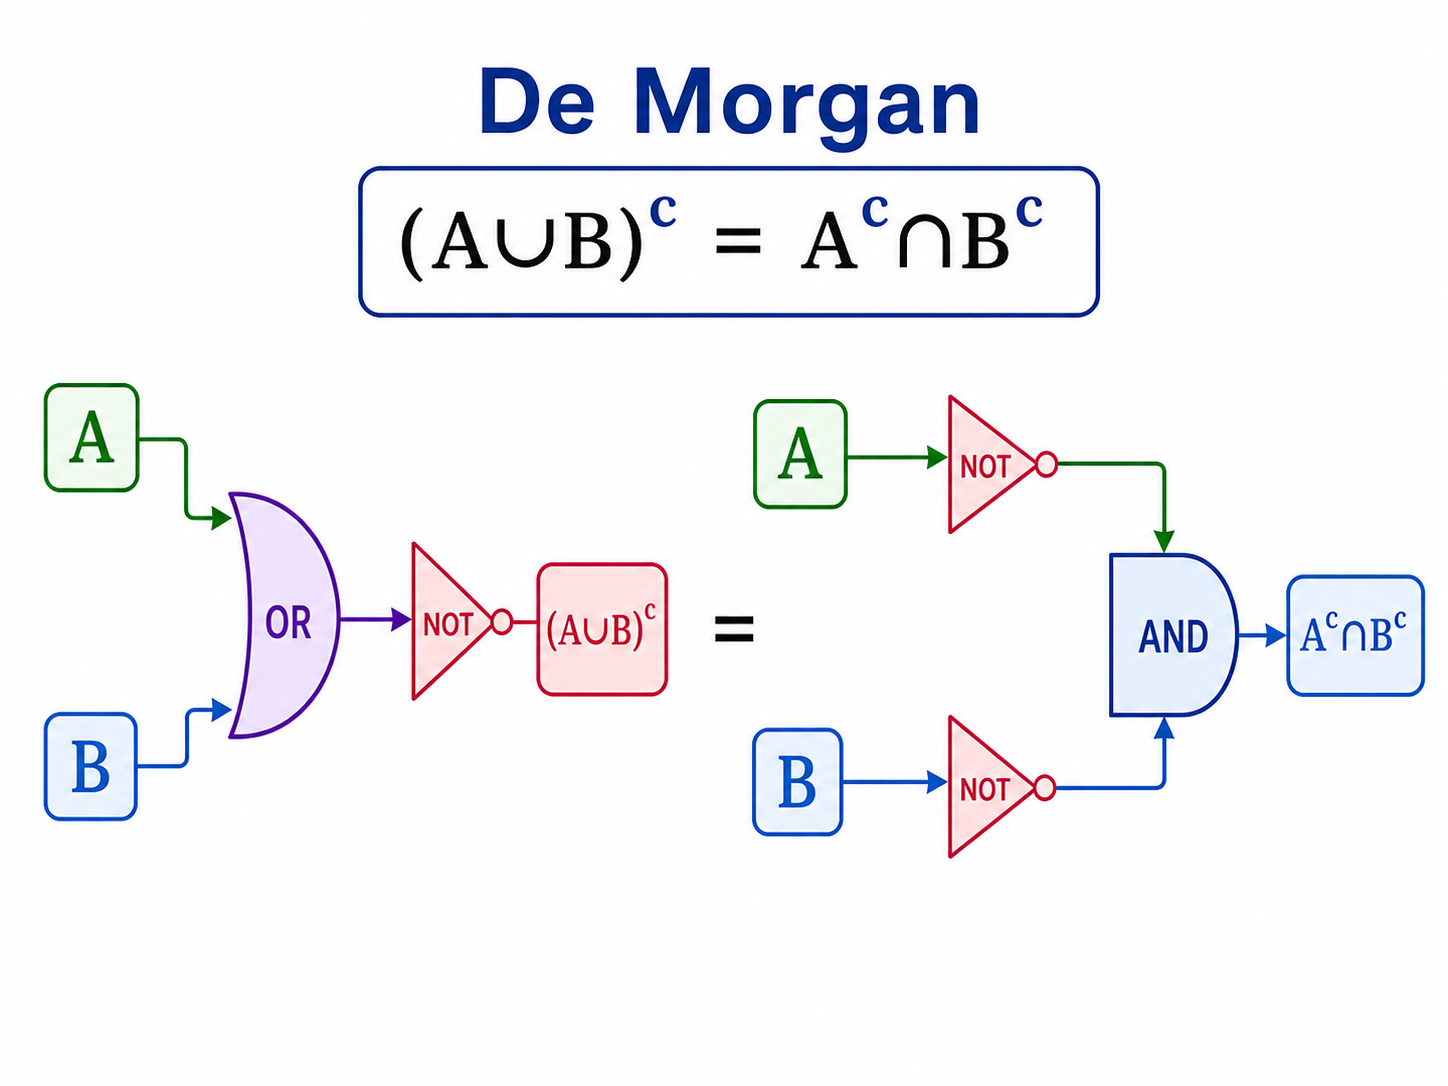
\includegraphics[width=0.82\textwidth]{Figures/png_ready/demorgan-laws-generated.png}
    \caption{กฎเดอมอร์แกน}
    \label{fig:boolean-demorgan-flow}
\end{figure}

\begin{rem}
สังเกตความสอดคล้องกับกฎเดอมอร์แกนในตรรกศาสตร์และทฤษฎีเซต ดังนี้

\begin{enumerate}
    \item $\neg(p \lor q) \equiv \neg p \land \neg q$ สอดคล้องกับ $(a + b)' = a' \cdot b'$
    \item $\neg(p \land q) \equiv \neg p \lor \neg q$ สอดคล้องกับ $(a \cdot b)' = a' + b'$
\end{enumerate}
นี่เป็นตัวอย่างที่แสดงความเชื่อมโยงระหว่างตรรกศาสตร์ ทฤษฎีเซต และพีชคณิตบูลีน
\end{rem}

\section{นิพจน์บูลีนและฟังก์ชันบูลีน (Boolean Expressions and Functions)}
\label{sec:boolean-expressions}
นิพจน์บูลีนและฟังก์ชันบูลีนเป็นเครื่องมือสำคัญในการจำลองและวิเคราะห์ปัญหาทางตรรกศาสตร์ในระบบคอมพิวเตอร์ โดยฟังก์ชันบูลีน (Boolean Function) คือ การจับคู่ (Mapping) จากโดเมนของตัวแปรบูลีน $n$ ตัวแปร $B^n = \{0, 1\}^n$ ไปยังเรนจ์ $\{0, 1\}$ ความสัมพันธ์ของฟังก์ชันสามารถนำเสนอได้ทั้งในรูปของตารางค่าความจริง นิพจน์พีชคณิต และแผนภาพการไหลของสัญญาณ ดังแสดงในรูปที่~\ref{fig:function-mapping}~\parencite{mano2018digital}

รูปที่~\ref{fig:function-mapping} แสดงตัวอย่างการทำงานของฟังก์ชันบูลีน 2 ฟังก์ชันแยกจากกัน โดยแถวบนรับตัวแปรขาเข้า $x$ และ $y$ เพื่อคำนวณ $F = x \cdot y$ (ฟังก์ชัน AND) ส่วนแถวล่างรับตัวแปรขาเข้า $x$ เพื่อคำนวณ $F = \bar{x}$ (ฟังก์ชัน NOT) สัญลักษณ์ $F$ ในแต่ละแถวจึงหมายถึงค่าสัญญาณขาออกของฟังก์ชันนั้น ๆ

\begin{figure}[H]
    \centering
    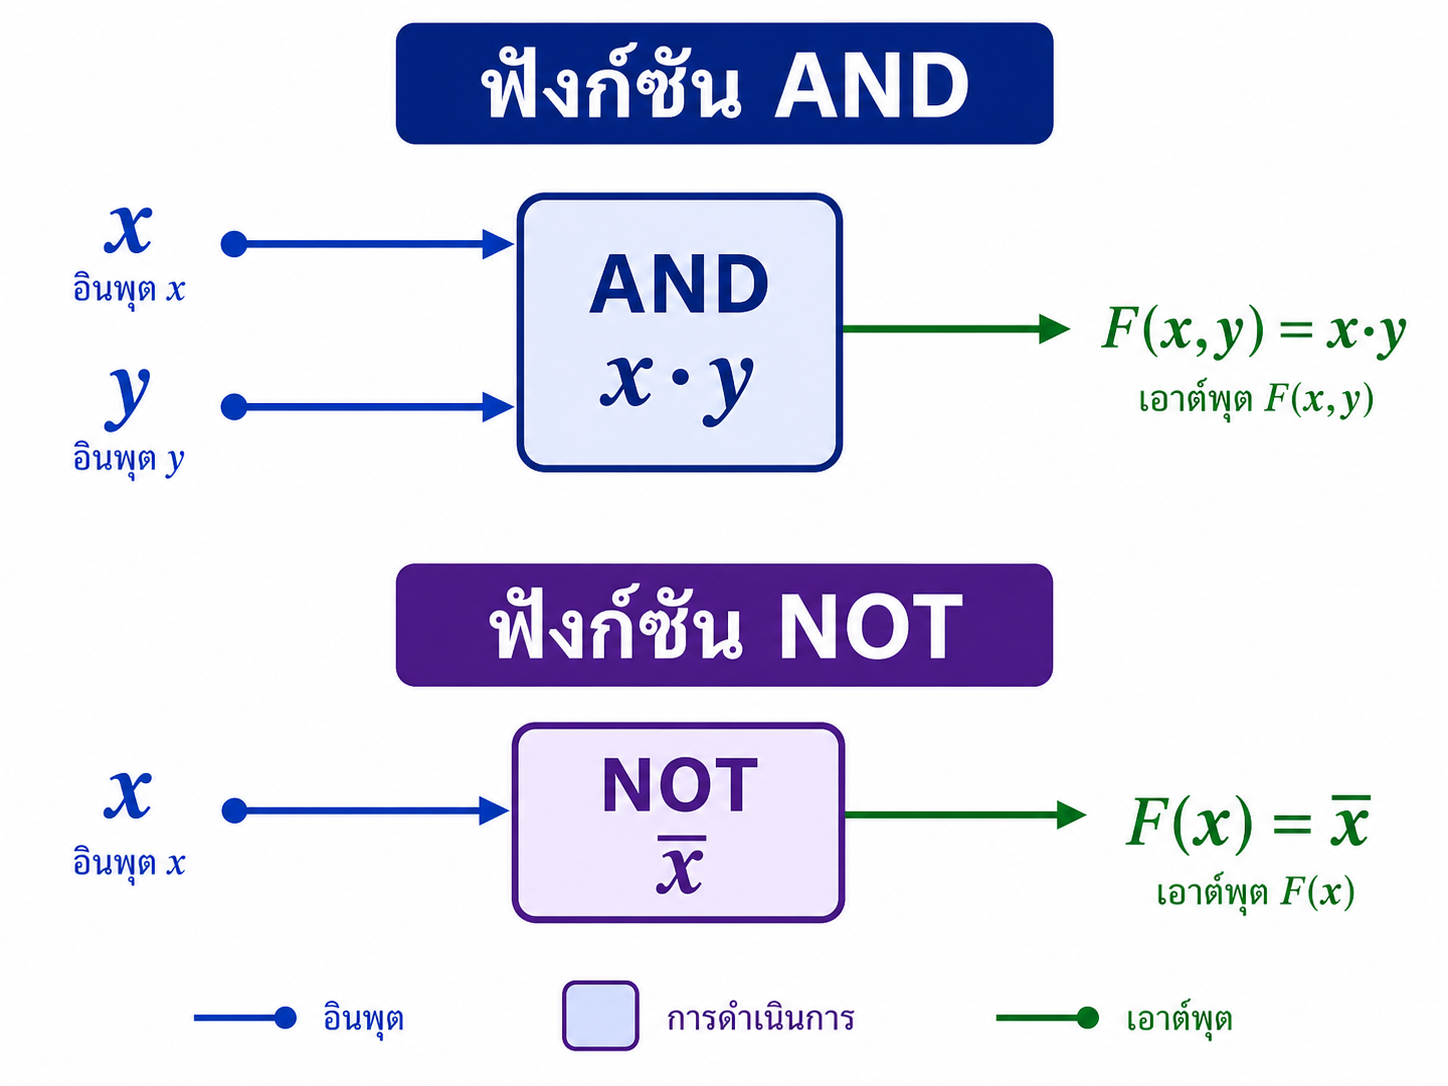
\includegraphics[width=0.78\textwidth]{Figures/png_ready/boolean-function-flow-labeled.png}
    \caption{ตัวอย่างการไหลของอินพุตสำหรับฟังก์ชัน AND และ NOT แยกกัน}
    \label{fig:function-mapping}
\end{figure}

นิพจน์บูลีนประกอบด้วยตัวแปรบูลีน ค่าคงตัว 0 และ 1 พร้อมด้วยตัวดำเนินการ OR, AND และ NOT โดยใช้วงเล็บเพื่อควบคุมลำดับการประมวลผล ฟังก์ชันบูลีนสามารถแสดงผลได้ในหลายรูปแบบ เช่น ตารางค่าความจริง นิพจน์บูลีน และแผนที่คาร์นอ (Karnaugh Map)

ในกระบวนการออกแบบวงจรดิจิทัล ฟังก์ชันบูลีนทำหน้าที่เป็นแบบจำลองเริ่มต้น โดยผู้ออกแบบจะแปลงข้อกำหนดของระบบให้เป็นฟังก์ชันบูลีน จากนั้นจึงดำเนินการลดรูปนิพจน์ให้มีจำนวนพจน์และตัวแปรน้อยที่สุดก่อนนำไปสังเคราะห์เป็นวงจรฮาร์ดแวร์จริง ซึ่งช่วยลดจำนวนอุปกรณ์อิเล็กทรอนิกส์และเกตทางตรรกะ ส่งผลให้วงจรมีขนาดเล็กลง ประหยัดพลังงาน และลดต้นทุนการผลิต

\subsection{นิยามของนิพจน์บูลีน}
นิพจน์บูลีน (Boolean Expression) คือ การนำตัวแปรบูลีน ค่าคงตัว ($0$ และ $1$) และตัวดำเนินการทางตรรกศาสตร์ ($+$, $\cdot$, $'$) มาประกอบเข้าด้วยกันอย่างถูกต้องตามหลักไวยากรณ์ โดยใช้วงเล็บเพื่อกำหนดลำดับการคำนวณ การทำความเข้าใจโครงสร้างและลำดับความสำคัญของตัวดำเนินการในนิพจน์บูลีนเป็นพื้นฐานสำคัญในการวิเคราะห์และสร้างวงจรดิจิทัล~\parencite{mano2018digital}

\begin{definition}[นิพจน์บูลีน]
\index{นิพจน์บูลีน!นิยาม}
นิพจน์บูลีน คือการรวมกันขององค์ประกอบต่อไปนี้
\begin{enumerate}
    \item ตัวแปรบูลีน เช่น $x, y, z$
    \item ค่าคงตัวบูลีน 0 และ 1
    \item การดำเนินการบูลีน ($+$, $\cdot$, $'$)
    \item วงเล็บ $($ และ $)$ เพื่อกำหนดลำดับการดำเนินการ
\end{enumerate}
\end{definition}

\begin{ex}[การจำแนกนิพจน์บูลีนที่ถูกต้องตามกฎการสร้าง]
\label{ex:valid-expressions}
จงตรวจสอบว่านิพจน์ต่อไปนี้เป็นนิพจน์บูลีนที่ถูกต้องตามกฎการสร้างหรือไม่ พร้อมระบุลำดับการดำเนินการ

\begin{enumerate}
    \item $x + y$
    \item $x \cdot y'$
    \item $(x + y) \cdot z$
    \item $x' + y \cdot z$
    \item $(a + b) \cdot (a' + c) + (a \cdot b \cdot c)'$
\end{enumerate}
\end{ex}
\begin{solution}
ทุกนิพจน์สร้างจากตัวแปรบูลีนกับตัวดำเนินการ $+,\ \cdot,\ '$ ตามกฎการสร้างนิพจน์ (ลำดับความสำคัญคือ $'$ ก่อน $\cdot$ ก่อน $+$; วงเล็บกำหนดลำดับได้) $\therefore$ ทั้งห้าเป็นนิพจน์บูลีนที่ถูกต้อง \solhere
\end{solution}

\subsection{ฟังก์ชันบูลีน}
ฟังก์ชันบูลีน (Boolean Function) คือ ฟังก์ชันที่รับค่าตัวแปรขาเข้าเป็นชุดข้อมูลบูลีน และให้ผลลัพธ์ขาออกเป็นค่าบูลีนเพียงค่าเดียว ฟังก์ชันที่มีตัวแปรจำนวน $n$ ตัวจะถูกกำหนดพฤติกรรมได้อย่างสมบูรณ์ด้วยตารางค่าความจริงขนาด $2^n$ แถว ซึ่งแสดงว่าสำหรับตัวแปรจำนวนจำกัด จะมีฟังก์ชันบูลีนที่เป็นไปได้ทั้งหมดจำนวนจำกัดเท่ากับ $2^{2^n}$ ฟังก์ชัน สมบัตินี้ช่วยให้สามารถตรวจสอบความถูกต้องของการทำงานของวงจรได้อย่างครบถ้วนทุกกรณี~\parencite{mano2018digital}

\begin{definition}[ฟังก์ชันบูลีน]
\index{ฟังก์ชันบูลีน!นิยาม}
ฟังก์ชันบูลีน $f(x_1, x_2, \ldots, x_n)$ คือ ฟังก์ชันที่รับค่าบูลีน $n$ ตัวแปรและให้ผลลัพธ์เป็นค่าบูลีน
\end{definition}

ฟังก์ชันบูลีนสามารถแทนด้วยตารางค่าความจริงที่แสดงผลลัพธ์สำหรับทุกชุดค่าอินพุตที่เป็นไปได้

\begin{ex}[การสร้างตารางค่าความจริงของฟังก์ชันสองตัวแปร]
\label{ex:truth-table-2var}
จงสร้างตารางค่าความจริงของ $f(x, y) = x \cdot y + x' \cdot y'$ แล้วระบุว่าฟังก์ชันนี้ตรงกับการดำเนินการมาตรฐานชนิดใด
\end{ex}
\begin{solution}
สร้างตารางค่าความจริงของฟังก์ชัน
\begin{center}
\begin{tabular}{|c|c|c|c|c|c|}
\hline
$x$ & $y$ & $x'$ & $y'$ & $x \cdot y$ & $x \cdot y + x' \cdot y'$ \\
\hline
0 & 0 & 1 & 1 & 0 & 1 \\
\hline
0 & 1 & 1 & 0 & 0 & 0 \\
\hline
1 & 0 & 0 & 1 & 0 & 0 \\
\hline
1 & 1 & 0 & 0 & 1 & 1 \\
\hline
\end{tabular}
\end{center}
$f = 1$ เมื่อ $x = y$ และ $f = 0$ เมื่อ $x \neq y$ $\therefore f$ คือฟังก์ชัน \textbf{XNOR} \solhere
\end{solution}

\begin{ex}[การสร้างตารางค่าความจริงของฟังก์ชันสามตัวแปร]
\label{ex:truth-table-3var}
จงสร้างตารางค่าความจริงของ $f(x, y, z) = (x + y') \cdot z + x \cdot y$ โดยแยกคอลัมน์ของแต่ละพจน์ย่อยเพื่อลดความผิดพลาด
\end{ex}
\begin{solution}
สร้างตารางค่าความจริงของฟังก์ชัน
\begin{center}
\begin{tabular}{|c|c|c|c|c|c|c|c|}
\hline
$x$ & $y$ & $z$ & $y'$ & $x + y'$ & $(x + y') \cdot z$ & $x \cdot y$ & $f$ \\
\hline
0 & 0 & 0 & 1 & 1 & 0 & 0 & 0 \\
\hline
0 & 0 & 1 & 1 & 1 & 1 & 0 & 1 \\
\hline
0 & 1 & 0 & 0 & 0 & 0 & 0 & 0 \\
\hline
0 & 1 & 1 & 0 & 0 & 0 & 0 & 0 \\
\hline
1 & 0 & 0 & 1 & 1 & 0 & 0 & 0 \\
\hline
1 & 0 & 1 & 1 & 1 & 1 & 0 & 1 \\
\hline
1 & 1 & 0 & 0 & 1 & 0 & 1 & 1 \\
\hline
1 & 1 & 1 & 0 & 1 & 1 & 1 & 1 \\
\hline
\end{tabular}
\end{center}

$\therefore$ ตารางค่าความจริงของ $f$ ครบทั้งแปดแถวตามที่แสดง \solhere
\end{solution}

\section{รูปแบบบัญญัติ (Canonical Forms)}
\label{sec:canonical-forms}

รูปแบบบัญญัติ (Canonical Forms) เป็นวิธีมาตรฐานสากลในการแสดงฟังก์ชันบูลีนให้อยู่ในโครงสร้างที่เป็นเอกลักษณ์และเป็นระบบ โดยฟังก์ชันบูลีนใด ๆ สามารถเขียนแสดงในรูปแบบบัญญัติได้ 2 รูปแบบหลัก ได้แก่ รูปแบบผลบวกของผลคูณ (Sum of Products: SOP) และรูปแบบผลคูณของผลบวก (Product of Sums: POS) การเขียนฟังก์ชันในรูปแบบบัญญัตินอกจากจะช่วยให้สามารถเปรียบเทียบความสมมูลของฟังก์ชันได้อย่างชัดเจนแล้ว ยังเป็นพื้นฐานสำคัญในการลดรูปนิพจน์ด้วยแผนที่คาร์นอ (Karnaugh Map)~\parencite{roth2021logic}

\subsection{มินเทอมและแมกซ์เทอม (Minterms and Maxterms)}
การทำความเข้าใจรูปแบบบัญญัติจำเป็นต้องอาศัยแนวคิดพื้นฐานของ \textbf{มินเทอม (Minterm)} และ \textbf{แมกซ์เทอม (Maxterm)} โดยมินเทอมคือพจน์ผลคูณ (AND Term) ที่ประกอบด้วยตัวแปรทุกตัวในฟังก์ชันปรากฏเพียงครั้งเดียว (หากตัวแปรมีค่าเป็น 1 จะแทนด้วยตัวแปรปกติ แต่หากมีค่าเป็น 0 จะแทนด้วยคอมพลีเมนต์) ในทางตรงกันข้าม แมกซ์เทอมคือพจน์ผลบวก (OR Term) ที่ประกอบด้วยตัวแปรทุกตัวปรากฏเพียงครั้งเดียว โดยหากตัวแปรมีค่าเป็น 0 จะแทนด้วยตัวแปรปกติ และหากมีค่าเป็น 1 จะแทนด้วยคอมพลีเมนต์ ความสัมพันธ์ระหว่างมินเทอมและแมกซ์เทอมช่วยให้สามารถแปลงรูปฟังก์ชันระหว่าง SOP และ POS ได้อย่างเป็นระบบ~\parencite{wakerly2018digital}

\begin{definition}[มินเทอม]
\index{มินเทอม!นิยาม}
มินเทอม ของตัวแปร $n$ ตัวคือ AND term ที่มีตัวแปรทุกตัวปรากฏเพียงครั้งเดียวในรูปแบบบัญญัติ (ถ้าตัวแปรเป็น 1 ใช้ตัวแปรเดี่ยว ถ้าตัวแปรเป็น 0 ใช้คอมพลีเมนต์)

สำหรับ 2 ตัวแปร $x, y$ ได้ดังนี้
\begin{enumerate}
    \item $m_0 = x' \cdot y'$ (ทั้ง $x = 0, y = 0$)
    \item $m_1 = x' \cdot y$ (ทั้ง $x = 0, y = 1$)
    \item $m_2 = x \cdot y'$ (ทั้ง $x = 1, y = 0$)
    \item $m_3 = x \cdot y$ (ทั้ง $x = 1, y = 1$)
\end{enumerate}
\end{definition}

\begin{definition}[แมกซ์เทอม]
\index{แมกซ์เทอม!นิยาม}
แมกซ์เทอม ของตัวแปร $n$ ตัวคือ OR term ที่มีตัวแปรทุกตัวปรากฏเพียงครั้งเดียวในรูปแบบบัญญัติ (ถ้าตัวแปรเป็น 0 ใช้ตัวแปรเดี่ยว ถ้าตัวแปรเป็น 1 ใช้คอมพลีเมนต์)

สำหรับ 2 ตัวแปร $x, y$ ได้ดังนี้
\begin{enumerate}
    \item $M_0 = x + y$ (ทั้ง $x = 0, y = 0$)
    \item $M_1 = x + y'$ (ทั้ง $x = 0, y = 1$)
    \item $M_2 = x' + y$ (ทั้ง $x = 1, y = 0$)
    \item $M_3 = x' + y'$ (ทั้ง $x = 1, y = 1$)
\end{enumerate}
\end{definition}

\begin{prop}
ความสัมพันธ์ระหว่าง Minterm และ Maxterm โดยที่ $m_i$ และ $M_i$ แทนมินเทอมและแมกซ์เทอมลำดับที่ $i$ ตามลำดับ
\begin{enumerate}
    \item $m_i = M_i'$
    \item $M_i = m_i'$
    \item $\sum$ (sigma) ใช้แทน sum ของ minterms
    \item $\prod$ (pi) ใช้แทน product ของ maxterms
\end{enumerate}
\end{prop}

\subsection{ผลบวกของผลคูณ (Sum of Products -- SOP)}
รูปแบบผลบวกของผลคูณ (Sum of Products: SOP) เป็นโครงสร้างมาตรฐานที่นิยมใช้ในการออกแบบวงจรดิจิทัล โดยเกิดจากการนำพจน์มินเทอมของแถวที่ฟังก์ชันให้ผลลัพธ์เป็น 1 มารวมกันด้วยตัวดำเนินการ OR (ผลบวกของกลุ่มผลคูณ AND) โครงสร้างในรูปแบบ SOP มีบทบาทสำคัญเนื่องจากสามารถนำไปสังเคราะห์เป็นวงจรดิจิทัลระดับ 2 ชั้น (Two-Level Logic Circuit) ที่ประกอบด้วยเกต AND ในชั้นแรกและเกต OR ในชั้นสุดท้ายได้อย่างสะดวกรวดเร็ว~\parencite{kolman2008discrete}

\begin{definition}[รูปแบบผลบวกของผลคูณ (SOP)]
\index{รูปแบบผลบวกของผลคูณ!นิยาม}
รูปแบบผลบวกของผลคูณ (Sum of Products: SOP) คือ รูปแบบของนิพจน์บูลีนที่เขียนเป็น OR ของ AND terms โดยฟังก์ชันบูลีนใด ๆ สามารถเขียนเป็น SOP ได้โดยใช้ minterm expansion
\end{definition}

\begin{ex}[การเขียนฟังก์ชันในรูปแบบบัญญัติ SOP]
\label{ex:canonical-sop}
เขียนฟังก์ชัน $f(x, y) = x \cdot y + x'$ ในรูปแบบ canonical SOP
\end{ex}
\begin{solution}
สร้างตารางค่าความจริงของฟังก์ชัน
\begin{center}
\begin{tabular}{|c|c|c|c|c|}
\hline
$x$ & $y$ & $x \cdot y$ & $x'$ & $f$ \\
\hline
0 & 0 & 0 & 1 & 1 \\
\hline
0 & 1 & 0 & 1 & 1 \\
\hline
1 & 0 & 0 & 0 & 0 \\
\hline
1 & 1 & 1 & 0 & 1 \\
\hline
\end{tabular}
\end{center}
แถวที่ $f = 1$ ได้แก่ $(0,0), (0,1), (1,1)$ ตรงกับ $m_0 = x'y',\ m_1 = x'y,\ m_3 = xy$
\[
\therefore f(x, y) = x'y' + x'y + xy = \sum(0, 1, 3)
\]
\solhere
\end{solution}

\begin{ex}[การเขียน SOP จากรายการมินเทอม]
\label{ex:sop-from-minterms}
กำหนดให้ตารางค่าความจริงของ $f(x, y, z)$ มีค่า $f = 1$ ที่มินเทอม $m_1, m_3, m_5, m_7$ จงเขียน $f$ ในรูปแบบบัญญัติ SOP
\end{ex}
\begin{solution}
\begin{align*}
m_1 = 001 &\Rightarrow x'y'z & m_3 = 011 &\Rightarrow x'yz\\
m_5 = 101 &\Rightarrow xy'z & m_7 = 111 &\Rightarrow xyz
\end{align*}
$\therefore f(x, y, z) = x'y'z + x'yz + xy'z + xyz = \sum(1, 3, 5, 7)$ \solhere
\end{solution}

\subsection{ผลคูณของผลบวก (Product of Sums -- POS)}
รูปแบบผลคูณของผลบวก (Product of Sums: POS) เป็นอีกหนึ่งโครงสร้างมาตรฐาน โดยเกิดจากการนำพจน์แมกซ์เทอมของแถวที่ฟังก์ชันให้ผลลัพธ์เป็น 0 มารวมกันด้วยตัวดำเนินการ AND (ผลคูณของกลุ่มผลบวก OR) โครงสร้างในรูปแบบ POS มีประโยชน์ในการออกแบบวงจรที่ใช้เกต OR ในชั้นแรกตามด้วยเกต AND ในชั้นถัดไป หรือการสังเคราะห์วงจรด้วยเกต NOR ล้วน การทำความเข้าใจทั้งรูปแบบ SOP และ POS จะช่วยให้ผู้ออกแบบสามารถเลือกโครงสร้างที่ประหยัดจำนวนเกตและเหมาะสมกับลักษณะของปัญหาได้ดียิ่งขึ้น~\parencite{gersting2014structures}

\begin{definition}[รูปแบบผลคูณของผลบวก (POS)]
\index{รูปแบบผลคูณของผลบวก!นิยาม}
รูปแบบผลคูณของผลบวก (Product of Sums: POS) คือ รูปแบบของนิพจน์บูลีนที่เขียนเป็น AND ของ OR terms โดยฟังก์ชันบูลีนใด ๆ สามารถเขียนเป็น POS ได้โดยใช้ maxterm expansion
\end{definition}

\begin{ex}[การเขียนฟังก์ชันในรูปแบบบัญญัติ POS]
\label{ex:canonical-pos}
เขียนฟังก์ชัน $f(x, y) = xy$ ในรูปแบบบัญญัติ POS
\end{ex}
\begin{solution}
สร้างตารางค่าความจริงของฟังก์ชัน แล้วมองหาแถวที่ $f = 0$ เพราะ POS สร้างจากแมกซ์เทอมของแถวเหล่านั้น
\begin{center}
\begin{tabular}{|c|c|c|c|}
\hline
$x$ & $y$ & $f = xy$ & แมกซ์เทอมของแถวที่ $f=0$ \\
\hline
0 & 0 & 0 & $M_0 = x + y$ \\
\hline
0 & 1 & 0 & $M_1 = x + y'$ \\
\hline
1 & 0 & 0 & $M_2 = x' + y$ \\
\hline
1 & 1 & 1 & --- \\
\hline
\end{tabular}
\end{center}
วิธีสร้างแมกซ์เทอมของแต่ละแถวคือ ตัวแปรที่มีค่าเป็น 0 ในแถวนั้นให้เขียนตัวมันเอง ส่วนตัวแปรที่มีค่าเป็น 1 ให้เขียนนิเสธ แล้วนำมา OR กัน ซึ่งทำให้แมกซ์เทอมนั้นมีค่าเป็น 0 เฉพาะแถวของตัวเองเท่านั้น · แถวที่ $f = 0$ ได้แก่ $(0,0), (0,1), (1,0)$
\[
\therefore f(x, y) = M_0 \cdot M_1 \cdot M_2 = \prod(0, 1, 2) = (x + y)(x + y')(x' + y)
\]
\solhere
\end{solution}

\begin{prop}
ความสัมพันธ์ระหว่าง SOP และ POS โดยที่ $\sum$ แทนผลบวกของ minterms และ $\prod$ แทนผลคูณของ maxterms:
ถ้า $f(x_1, \ldots, x_n) = \sum(m_{i_1}, m_{i_2}, \ldots)$ แล้ว $f(x_1, \ldots, x_n) = \prod(M_{j_1}, M_{j_2}, \ldots)$

โดยที่ $\{j_1, j_2, \ldots\}$ คือ maxterms ที่ไม่อยู่ใน minterm list
\end{prop}

\section{การลดรูปนิพจน์บูลีน (Boolean Expression Simplification)}
\label{sec:boolean-simplification}

นิพจน์บูลีนที่มีตารางค่าความจริงเหมือนกันทุกแถวจัดเป็นนิพจน์ที่สมมูลกันในเชิงตรรกศาสตร์ แต่เมื่อนำไปสังเคราะห์เป็นวงจรฮาร์ดแวร์จริง นิพจน์ที่ต่างรูปแบบกันจะใช้จำนวนลอจิกเกตและสายสัญญาณไม่เท่ากัน กระบวนการลดรูปนิพจน์บูลีน (Boolean Expression Simplification) จึงมีเป้าหมายเพื่อแปลงนิพจน์ให้อยู่ในรูปแบบที่สมมูลกันแต่มีจำนวนพจน์และตัวแปรน้อยที่สุด ส่งผลให้วงจรดิจิทัลมีขนาดเล็กลง ใช้พลังงานต่ำลง และลดเวลาหน่วงในการแพร่สัญญาณ (Propagation Delay) หัวข้อนี้จะนำเสนอการลดรูป 2 วิธีการ ได้แก่ การใช้กฎพีชคณิตบูลีน และการใช้ทฤษฎีบทคอนเซนซัส~\parencite{mano2018digital}

\subsection{การลดรูปด้วยกฎพีชคณิตบูลีน}
การลดรูปด้วยกฎและเอกลักษณ์ทางพีชคณิตบูลีนอาศัยการจัดกลุ่มพจน์ การดึงตัวประกอบร่วมด้วยกฎการแจกแจง และการตัดทอนตัวแปรด้วยกฎคอมพลีเมนต์และกฎการดูดกลืน ซึ่งช่วยลดจำนวนตัวแปรนำเข้า (Literal Count) และจำนวนเกตในวงจรดิจิทัลได้อย่างเป็นขั้นตอน~\parencite{mano2018digital}

\begin{ex}[การลดรูปด้วยกฎพีชคณิตบูลีน]
\label{ex:simplify-basic}
ลดรูป $f(x, y, z) = x y + x' y + x y'$
\end{ex}
\begin{solution}
\begin{align*}
f &= x y + x' y + x y' \\
  &= y(x + x') + x y' \quad \text{(Distributive ย้อนกลับ)} \\
  &= y \cdot 1 + x y' \quad \text{(กฎคอมพลีเมนต์ } x + x' = 1) \\
  &= y + x y' \\
  &= (y + x)(y + y') \quad \text{(Distributive)} \\
  &= (y + x) \cdot 1 \quad \text{(Complement)} \\
  &= x + y
\end{align*}
$\therefore f = x + y$ \solhere
\end{solution}

\begin{ex}[การลดรูปนิพจน์สามตัวแปร]
\label{ex:simplify-3var}
ลดรูป $f(a, b, c) = a b c + a b c' + a' b + a b' c$
\end{ex}
\begin{solution}
\begin{align*}
f &= a b c + a b c' + a' b + a b' c \\
  &= a b(c + c') + a' b + a b' c \quad \text{(Distributive)} \\
  &= a b \cdot 1 + a' b + a b' c \quad \text{(Complement)} \\
  &= a b + a' b + a b' c \\
  &= b(a + a') + a b' c \\
  &= b + a b' c \quad \text{(Complement)} \\
  &= (b + a)(b + b')(b + c) \quad \text{(Distributive)} \\
  &= (b + a) \cdot 1 \cdot (b + c) \quad \text{(Complement)} \\
  &= b + a c \quad \text{(Distributive ย้อนกลับ)}
\end{align*}
$\therefore f = b + a c$ \solhere
\end{solution}

\begin{ex}[การลดรูปนิพจน์ในรูปผลคูณของผลบวก]
\label{ex:simplify-pos-form}
ลดรูป $f(x, y) = (x + y) \cdot (x + y')$
\end{ex}
\begin{solution}
\begin{align*}
f &= (x + y) \cdot (x + y') \\
  &= x + y \cdot y' \quad \text{(Distribution: } x + yz = (x+y)(x+z)) \\
  &= x + 0 \quad \text{(กฎคอมพลีเมนต์ } y \cdot y' = 0) \\
  &= x
\end{align*}
$\therefore f = x$ \solhere
\end{solution}

\begin{ex}[การลดรูปอย่างละเอียดทีละขั้นตอน]
\label{ex:simplify-stepwise}
ลดรูปนิพจน์บูลีน $f(a, b, c) = (a + b) \cdot (a' + c) + (b + c)$ อย่างละเอียดทีละขั้นตอน
\end{ex}

\begin{solution}
\begin{align*}
f &= (a + b)(a' + c) + (b + c) \\
  &= a a' + b a' + a c + b c + b + c \quad \text{(Distributive)} \\
  &= b a' + a c + b c + b + c \quad \text{(กฎคอมพลีเมนต์ } a a' = 0) \\
  &= b a' + a c + b(1 + c) + c \\
  &= b a' + a c + b + c \quad \text{(Domination: } 1 + c = 1) \\
  &= b(a' + 1) + a c + c \\
  &= b + c(a + 1) \quad \text{(Domination)} \\
  &= b + c \quad \text{(Domination)}
\end{align*}
$\therefore f = b + c$ \solhere
\end{solution}

ตรวจสอบผลการลดรูปโดยไล่ค่าอินพุตทั้งแปดกรณี เทียบนิพจน์เดิมกับนิพจน์ที่ลดรูปแล้ว
\begin{center}
\begin{tabular}{|c|c|c|c|c|}
\hline
$a$ & $b$ & $c$ & $f = (a+b)(a'+c) + (b+c)$ & $b + c$ \\
\hline
0 & 0 & 0 & 0 & 0 \\
\hline
0 & 0 & 1 & 1 & 1 \\
\hline
0 & 1 & 0 & 1 & 1 \\
\hline
0 & 1 & 1 & 1 & 1 \\
\hline
1 & 0 & 0 & 0 & 0 \\
\hline
1 & 0 & 1 & 1 & 1 \\
\hline
1 & 1 & 0 & 1 & 1 \\
\hline
1 & 1 & 1 & 1 & 1 \\
\hline
\end{tabular}
\end{center}

สองคอลัมน์สุดท้ายมีค่าเท่ากันทุกแถว จึงยืนยันได้ว่าการลดรูปถูกต้อง ให้สังเกตด้วยว่าตัวแปร $a$ หายไปจากคำตอบทั้งที่ปรากฏในนิพจน์เดิมถึงสามที่ นี่คือประโยชน์ของการลดรูป คือวงจรจริงไม่ต้องรับสัญญาณ $a$ เข้ามาเลย

\subsection{การลดรูปด้วยทฤษฎีบทคอนเซนซัส (Consensus Theorem)}
ทฤษฎีบทคอนเซนซัส (Consensus Theorem) เป็นเครื่องมือสำคัญในการตัดพจน์ส่วนเกิน (Redundant Term) ออกจากนิพจน์บูลีน โดยระบุว่าเมื่อมีพจน์คูณ 2 พจน์ที่ประกอบด้วยตัวแปรหนึ่งในรูปปกติ ($a$) และอีกพจน์หนึ่งอยู่ในรูปคอมพลีเมนต์ ($a'$) พจน์ที่สามซึ่งเกิดจากผลคูณของตัวแปรที่เหลือในทั้งสองพจน์ ($bc$) จะถือเป็นพจน์คอนเซนซัสและสามารถตัดทิ้งได้โดยไม่ทำให้ค่าความจริงของนิพจน์เปลี่ยนแปลง~\parencite{rosen2019discrete}

\begin{thrm}[Consensus Theorem]
\begin{enumerate}
    \item $a b + a' c + b c = a b + a' c$
    \item $(a + b)(a' + c)(b + c) = (a + b)(a' + c)$
\end{enumerate}
\end{thrm}

\begin{proof}
\textbf{พิสูจน์ข้อ 1} $a b + a' c + b c = a b + a' c$

แนวคิดคือขยายพจน์ $bc$ ด้วยกฎคอมพลีเมนต์แล้วใช้กฎการแจกแจง ดังนี้

\begin{align*}
a b + a' c + b c &= a b + a' c + b c \cdot 1 \\
                &= a b + a' c + b c (a + a') \quad \text{(กฎคอมพลีเมนต์ } a + a' = 1 \text{)} \\
                &= a b + a' c + a b c + a' b c \\
                &= a b(1 + c) + a' c(1 + b) \\
                &= a b + a' c \quad \text{(กฎครอบงำ } 1 + c = 1 \text{)}
\end{align*}

ดังนั้น $a b + a' c + b c = a b + a' c$ พิสูจน์แล้ว

หรือพิสูจน์ด้วยตารางค่าความจริง

\begin{center}
\begin{tabular}{|c|c|c|c|c|c|c|c|}
\hline
$a$ & $b$ & $c$ & $ab$ & $a'c$ & $bc$ & $ab+a'c+bc$ & $ab+a'c$ \\
\hline
0 & 0 & 0 & 0 & 0 & 0 & 0 & 0 \\
\hline
0 & 0 & 1 & 0 & 1 & 0 & 1 & 1 \\
\hline
0 & 1 & 0 & 0 & 0 & 0 & 0 & 0 \\
\hline
0 & 1 & 1 & 0 & 1 & 1 & 1 & 1 \\
\hline
1 & 0 & 0 & 0 & 0 & 0 & 0 & 0 \\
\hline
1 & 0 & 1 & 0 & 0 & 0 & 0 & 0 \\
\hline
1 & 1 & 0 & 1 & 0 & 0 & 1 & 1 \\
\hline
1 & 1 & 1 & 1 & 0 & 1 & 1 & 1 \\
\hline
\end{tabular}
\end{center}

เนื่องจากคอลัมน์ $ab + a'c + bc$ และ $ab + a'c$ มีค่าเท่ากันทุกแถว ดังนั้น $a b + a' c + b c = a b + a' c$

\medskip
\textbf{พิสูจน์ข้อ 2} $(a + b)(a' + c)(b + c) = (a + b)(a' + c)$

ข้อนี้เป็นคู่ทวิภาคของข้อ 1 พอดี เพราะได้จากการสลับ $+$ กับ $\cdot$ ทุกตำแหน่งโดยไม่เปลี่ยนตัวแปร ตามหลักการทวิภาคจึงเป็นจริงทันทีเมื่อข้อ 1 เป็นจริง อย่างไรก็ตาม การกระจายพจน์ตรง ๆ ก็ให้ผลเดียวกัน ดังนี้

เริ่มจากขยายตัวประกอบ $(b + c)$ ด้วยกฎคอมพลีเมนต์ $a a' = 0$ แล้วใช้กฎการแจกแจง
\begin{align*}
(b + c) = (b + c) + a a' = (a + b + c)(a' + b + c)
\end{align*}
แทนค่ากลับเข้าไปแล้วจัดหมู่ตัวประกอบใหม่ ได้
\begin{align*}
(a + b)(a' + c)(b + c) &= \bigl[(a + b)(a + b + c)\bigr]\bigl[(a' + c)(a' + b + c)\bigr]\\
                       &= (a + b)(a' + c)
\end{align*}
โดยขั้นสุดท้ายใช้กฎการดูดกลืนรูป $X(X + Y) = X$ สองครั้ง ครั้งแรกที่ $X = a + b$ กับ $Y = c$ และครั้งที่สองที่ $X = a' + c$ กับ $Y = b$

ดังนั้น $(a + b)(a' + c)(b + c) = (a + b)(a' + c)$ พิสูจน์แล้ว
\end{proof}

\begin{ex}[การลดรูปด้วยทฤษฎีบทคอนเซนซัส]
\label{ex:consensus-simplify}
ลดรูป $f(x, y, z) = x y + x' z + y z$
\end{ex}
\begin{solution}
\begin{align*}
f &= x y + x' z + y z \\
  &= x y + x' z \quad \text{(Consensus: } yz \text{ ถูกละทิ้ง)}
\end{align*}
$\therefore f = x y + x' z$ \solhere
\end{solution}

เพอร์เซปตรอน (Perceptron) เป็นแบบจำลองพื้นฐานที่สุดของโครงข่ายประสาทเทียม (Neural Networks) ซึ่งทำงานสอดคล้องกับหลักการคำนวณของลอจิกเกตในวงจรดิจิทัล โดยเพอร์เซปตรอนจะรับสัญญาณขาเข้า (Inputs) ถ่วงน้ำหนักด้วยค่าน้ำหนัก (Weights) รวมกับค่าไบแอส (Bias) แล้วส่งผ่านฟังก์ชันกระตุ้น (Activation Function) แบบขั้นบันได เพื่อตัดสินใจให้ค่าสัญญาณขาออกเป็น 0 หรือ 1

\begin{ex}[การคำนวณผลลัพธ์ของเพอร์เซปตรอน]
\label{ex:perceptron}
จงคำนวณ output ของ Perceptron ที่มี 2 inputs $x_1, x_2$ โดยมี weights $w_1 = 0.5$, $w_2 = 0.5$ และ bias $b = -0.7$ และใช้ step function เป็น activation:
$$f(z) = \begin{cases} 1 & \text{ถ้า } z \geq 0 \\ 0 & \text{ถ้า } z < 0 \end{cases}$$
โดยที่ $z = x_1 w_1 + x_2 w_2 + b$ จงทดสอบกับ input $(0, 0)$, $(0, 1)$, $(1, 0)$, $(1, 1)$
\end{ex}
\begin{solution}
คำนวณ $z = x_1 w_1 + x_2 w_2 + b$ แล้ว $y = f(z)$ ทีละกรณี
\begin{align*}
(0,0):\ z &= 0 + 0 - 0.7 = -0.7 < 0 &&\Rightarrow y = 0\\
(0,1):\ z &= 0 + 0.5 - 0.7 = -0.2 < 0 &&\Rightarrow y = 0\\
(1,0):\ z &= 0.5 + 0 - 0.7 = -0.2 < 0 &&\Rightarrow y = 0\\
(1,1):\ z &= 0.5 + 0.5 - 0.7 = 0.3 \geq 0 &&\Rightarrow y = 1
\end{align*}
$\therefore y = x_1 \land x_2$. Perceptron ตัวนี้ทำงานเหมือน AND gate โดย weight และ bias เรียนรู้ได้จากข้อมูลด้วย learning rule $w_i \leftarrow w_i + \eta (t - y) x_i$ \solhere
\end{solution}

\section{แผนที่คาร์นอ (Karnaugh Map)}
\label{sec:karnaugh-map}

แผนที่คาร์นอ (Karnaugh Map: K-map) พัฒนาขึ้นโดย มอริส คาร์นอ (Maurice Karnaugh) ในปี ค.ศ. 1953 เป็นเครื่องมือเชิงภาพ (Visual Tool) ที่ใช้ในการลดรูปฟังก์ชันบูลีนได้อย่างเป็นระบบ แผนที่คาร์นอจัดเรียงมินเทอมของฟังก์ชันลงในตาราง 2 มิติ โดยอาศัยหลักการของรหัสเกรย์ (Gray Code) เพื่อให้เซลล์ที่อยู่ติดกัน (Adjacent Cells) มีค่าตัวแปรแตกต่างกันเพียง 1 บิตเสมอ ส่งผลให้สามารถจับกลุ่มเซลล์ที่มีค่าเป็น 1 ที่อยู่ข้างเคียงกันในขนาดที่เป็นเลขยกกำลังของสอง ($1, 2, 4, 8, 16$ เซลล์) เพื่อกำจัดตัวแปรที่เปลี่ยนสถานะออกไปได้อย่างสะดวกรวดเร็ว การใช้แผนที่คาร์นอมีประสิทธิภาพสูงสำหรับฟังก์ชันที่มีตัวแปรตั้งแต่ 2 ถึง 4 ตัวแปร~\parencite{mano2018digital}

ข้อได้เปรียบสำคัญของแผนที่คาร์นอเมื่อเปรียบเทียบกับการใช้กฎพีชคณิตบูลีน คือ ความเป็นระบบที่ช่วยลดข้อผิดพลาดจากมนุษย์ และรับประกันได้ว่าจะได้นิพจน์ในรูปแบบผลบวกของผลคูณที่มีจำนวนพจน์น้อยที่สุด (Minimal SOP) สำหรับกรณีที่ฟังก์ชันมีตัวแปรมากกว่า 4 หรือ 5 ตัวแปรขึ้นไป จะนิยมใช้วิธีขั้นตอนวิธีเชิงตาราง เช่น วิธีไควน์-แมคคลัสกี (Quine-McCluskey Algorithm) ร่วมกับโปรแกรมคอมพิวเตอร์แทน

\subsection{แผนที่คาร์นอสำหรับ 2 ตัวแปร}
แผนที่คาร์นอสำหรับ 2 ตัวแปร ประกอบด้วย 4 เซลล์ ซึ่งสอดคล้องกับ 4 กรณีในตารางค่าความจริง โดยหัวแถวแทนตัวแปร $x$ และหัวคอลัมน์แทนตัวแปร $y$ เมื่อช่องที่อยู่ติดกันมีสถานะต่างกันเพียง 1 บิต การจับกลุ่มเซลล์ที่เป็น 1 สองช่องติดกันจึงสามารถตัดตัวแปรที่เปลี่ยนค่าออกไปได้ 1 ตัวแปร ทำให้เหลือพจน์ที่มีตัวแปรเพียงตัวเดียว~\parencite{roth2021logic}

\begin{principle}[รูปแบบแผนที่คาร์นอ 2 ตัวแปร]
แผนที่คาร์นอสำหรับ 2 ตัวแปร $x, y$ จัดเรียงดังนี้

\begin{center}
\begin{tabular}{|c|c|c|}
\hline
 & $y = 0$ & $y = 1$ \\
\hline
$x = 0$ & $m_0$ & $m_1$ \\
       & $x'y'$ & $x'y$ \\
\hline
$x = 1$ & $m_2$ & $m_3$ \\
       & $xy'$ & $xy$ \\
\hline
\end{tabular}
\end{center}

เซลล์ที่อยู่ติดกัน (adjacent cells) หมายถึงเซลล์ที่รหัสประจำช่องต่างกันเพียงหนึ่งบิต ซึ่งในแผนที่ 2 ตัวแปรตรงกับเซลล์ที่แชร์ขอบกันพอดี แต่ในแผนที่ที่ใหญ่กว่านี้ยังรวมถึงเซลล์ริมซ้ายกับริมขวา และเซลล์ริมบนกับริมล่างด้วย เพราะรหัสของคู่เหล่านั้นก็ต่างกันเพียงหนึ่งบิตเช่นกัน การจับกลุ่มข้ามขอบแบบนี้เรียกว่าการพันขอบ (wrap around) ซึ่งจะเห็นตัวอย่างในแผนที่ 3 และ 4 ตัวแปร
\end{principle}

\begin{principle}[ขั้นตอนและกฎการจับกลุ่มในแผนที่คาร์นอ]
\label{prin:kmap-rules}
การลดรูปด้วยแผนที่คาร์นอมีขั้นตอนดังนี้
\begin{enumerate}
    \item เขียนแผนที่ตามจำนวนตัวแปร โดยหัวแถวและหัวคอลัมน์เรียงด้วยรหัสเกรย์
    \item ใส่ 1 ในเซลล์ที่ตรงกับมินเทอมที่อยู่ในฟังก์ชัน ช่องที่เหลือใส่ 0
    \item จัดกลุ่มเซลล์ที่เป็น 1 ที่อยู่ติดกัน โดยขนาดกลุ่มต้องเป็นกำลังของสองเสมอ คือ 1, 2, 4, 8 ช่อง จะจับกลุ่มขนาด 3 หรือ 6 ช่องไม่ได้
    \item แต่ละกลุ่มต้องใหญ่ที่สุดเท่าที่จะเป็นไปได้ เพราะกลุ่มยิ่งใหญ่ยิ่งตัดตัวแปรออกได้มาก
    \item \textbf{ทุกช่องที่เป็น 1 ต้องถูกคลุมด้วยกลุ่มอย่างน้อยหนึ่งกลุ่ม} ถ้าเหลือช่องใดไม่ถูกคลุม นิพจน์ที่ได้จะไม่เท่ากับฟังก์ชันเดิม
    \item กลุ่มซ้อนทับกันได้ แต่ไม่ควรมีกลุ่มใดที่ทุกช่องถูกกลุ่มอื่นคลุมไปหมดแล้ว เพราะจะได้พจน์ที่ไม่จำเป็น
    \item หาตัวแปรที่มีค่าคงที่ตลอดทั้งกลุ่ม ตัวแปรที่คงที่เป็น 1 ให้เขียนตัวมันเอง ที่คงที่เป็น 0 ให้เขียนนิเสธ ส่วนตัวแปรที่เปลี่ยนค่าภายในกลุ่มให้ตัดทิ้ง
    \item นำพจน์ที่ได้จากทุกกลุ่มมา OR กัน
\end{enumerate}
\end{principle}


\begin{ex}[การลดรูปด้วยแผนที่คาร์นอ 2 ตัวแปร]
\label{ex:kmap-2var-a}
ใช้ K-map ลดรูป $f(x, y) = \sum(1, 2, 3)$

\begin{center}
\begin{tabular}{|c|c|c|}
\hline
 & $y = 0$ & $y = 1$ \\
\hline
$x = 0$ & 0 & 1 \\
       & $m_0$ & $m_1$ \\
\hline
$x = 1$ & 1 & 1 \\
       & $m_2$ & $m_3$ \\
\hline
\end{tabular}
\end{center}
\end{ex}
\begin{solution}
\begin{align*}
\{m_2, m_3\}\ (\text{แถว } x = 1) &\Rightarrow x\\
\{m_1, m_3\}\ (\text{คอลัมน์ } y = 1) &\Rightarrow y
\end{align*}
$\therefore f = x + y$ \solhere
\end{solution}

\begin{ex}[การลดรูปด้วยแผนที่คาร์นอ 2 ตัวแปรที่จับได้สองกลุ่ม]
\label{ex:kmap-2var-b}
ใช้ K-map ลดรูป $f(x, y) = x y + x y' + x' y'$

\begin{center}
\begin{tabular}{|c|c|c|}
\hline
 & $y = 0$ & $y = 1$ \\
\hline
$x = 0$ & 1 & 0 \\
       & $m_0$ & $m_1$ \\
\hline
$x = 1$ & 1 & 1 \\
       & $m_2$ & $m_3$ \\
\hline
\end{tabular}
\end{center}
\end{ex}
\begin{solution}
\begin{align*}
\{m_0, m_2\}\ (\text{คอลัมน์ } y = 0) &\Rightarrow y'\\
\{m_2, m_3\}\ (\text{แถว } x = 1) &\Rightarrow x
\end{align*}
$\therefore f = x + y'$ \solhere
\end{solution}

\subsection{แผนที่คาร์นอสำหรับ 3 ตัวแปร}
แผนที่คาร์นอสำหรับ 3 ตัวแปร ประกอบด้วย 8 เซลล์ จัดเรียงในรูปตาราง 2 แถวและ 4 คอลัมน์ โดยหัวแถวแทนตัวแปร $x$ ($0, 1$) และหัวคอลัมน์แทนคู่ตัวแปร $yz$ ซึ่งเรียงลำดับตามรหัสเกรย์เป็น $00, 01, 11, 10$ เพื่อให้เซลล์ในคอลัมน์ที่อยู่ติดกันต่างกันเพียง 1 บิตเสมอ~\parencite{wakerly2018digital}

\begin{principle}[รูปแบบแผนที่คาร์นอ 3 ตัวแปร]
แผนที่คาร์นอสำหรับ 3 ตัวแปร $x, y, z$ จัดเรียงดังนี้

\begin{center}
\begin{tabular}{|c|c|c|c|c|}
\hline
 & $yz = 00$ & $yz = 01$ & $yz = 11$ & $yz = 10$ \\
 & $y'z'$ & $y'z$ & $yz$ & $yz'$ \\
\hline
$x = 0$ & $m_0$ & $m_1$ & $m_3$ & $m_2$ \\
       & $x'y'z'$ & $x'y'z$ & $x'yz$ & $x'yz'$ \\
\hline
$x = 1$ & $m_4$ & $m_5$ & $m_7$ & $m_6$ \\
       & $xy'z'$ & $xy'z$ & $xyz$ & $xy z'$ \\
\hline
\end{tabular}
\end{center}

\textbf{หมายเหตุ} ลำดับของคอลัมน์ใช้ Gray code เพื่อให้เซลล์ข้างเคียงแตกต่างกันเพียง 1 bit
\end{principle}

\begin{ex}[การลดรูปด้วยแผนที่คาร์นอ 3 ตัวแปร]
\label{ex:kmap-3var}
ใช้ K-map ลดรูป $f(x, y, z) = \sum(0, 1, 3, 4, 5, 6)$

\begin{center}
\begin{tabular}{|c|c|c|c|c|}
\hline
 & $yz = 00$ & $yz = 01$ & $yz = 11$ & $yz = 10$ \\
\hline
$x = 0$ & 1 & 1 & 1 & 0 \\
\hline
$x = 1$ & 1 & 1 & 0 & 1 \\
\hline
\end{tabular}
\end{center}
\end{ex}
\begin{solution}
\begin{align*}
\{m_0, m_1, m_4, m_5\}\ (\text{บล็อก } 2\times 2 \text{ ซ้าย}) &\Rightarrow y'\\
\{m_1, m_3\}\ (\text{แถวบน},\ z = 1) &\Rightarrow x'z\\
\{m_4, m_6\}\ (\text{แถวล่าง wrap},\ z = 0) &\Rightarrow xz'
\end{align*}
$\therefore f = y' + x'z + xz'$ \solhere
\end{solution}

\subsection{แผนที่คาร์นอสำหรับ 4 ตัวแปร}
แผนที่คาร์นอสำหรับ 4 ตัวแปร ประกอบด้วย 16 เซลล์ จัดเรียงในรูปตาราง 4 แถวและ 4 คอลัมน์ โดยหัวแถวแทนคู่ตัวแปร $wx$ ($00, 01, 11, 10$) และหัวคอลัมน์แทนคู่ตัวแปร $yz$ ($00, 01, 11, 10$) การจัดเรียงตามรหัสเกรย์ทั้งสองแกนทำให้สามารถรวมกลุ่มเซลล์ข้างเคียงข้ามขอบตาราง (Wrap-Around) ได้ทั้งในแนวนอนและแนวตั้ง~\parencite{kolman2008discrete}

\begin{principle}[รูปแบบแผนที่คาร์นอ 4 ตัวแปร]
แผนที่คาร์นอสำหรับ 4 ตัวแปร $w, x, y, z$ จัดเรียงดังนี้

\begin{center}
\begin{tabular}{|c|c|c|c|c|}
\hline
 & $yz = 00$ & $yz = 01$ & $yz = 11$ & $yz = 10$ \\
 & $y'z'$ & $y'z$ & $yz$ & $yz'$ \\
\hline
$wx = 00$ & $m_0$ & $m_1$ & $m_3$ & $m_2$ \\
\hline
$wx = 01$ & $m_4$ & $m_5$ & $m_7$ & $m_6$ \\
\hline
$wx = 11$ & $m_{12}$ & $m_{13}$ & $m_{15}$ & $m_{14}$ \\
\hline
$wx = 10$ & $m_8$ & $m_9$ & $m_{11}$ & $m_{10}$ \\
\hline
\end{tabular}
\end{center}

การ wrap สามารถทำได้ทั้งในแนวนอนและแนวตั้ง (เช่น $m_0$ ติดกับ $m_1, m_2, m_4, m_8$)
\end{principle}

รูปที่~\ref{fig:kmap-grouping} เปรียบเทียบการจับกลุ่มที่ทำได้กับที่ทำไม่ได้ ให้สังเกตว่ากลุ่มต้องเป็นรูปสี่เหลี่ยมที่มีจำนวนช่องเป็นกำลังของสองเท่านั้น

\begin{figure}[H]
    \centering
    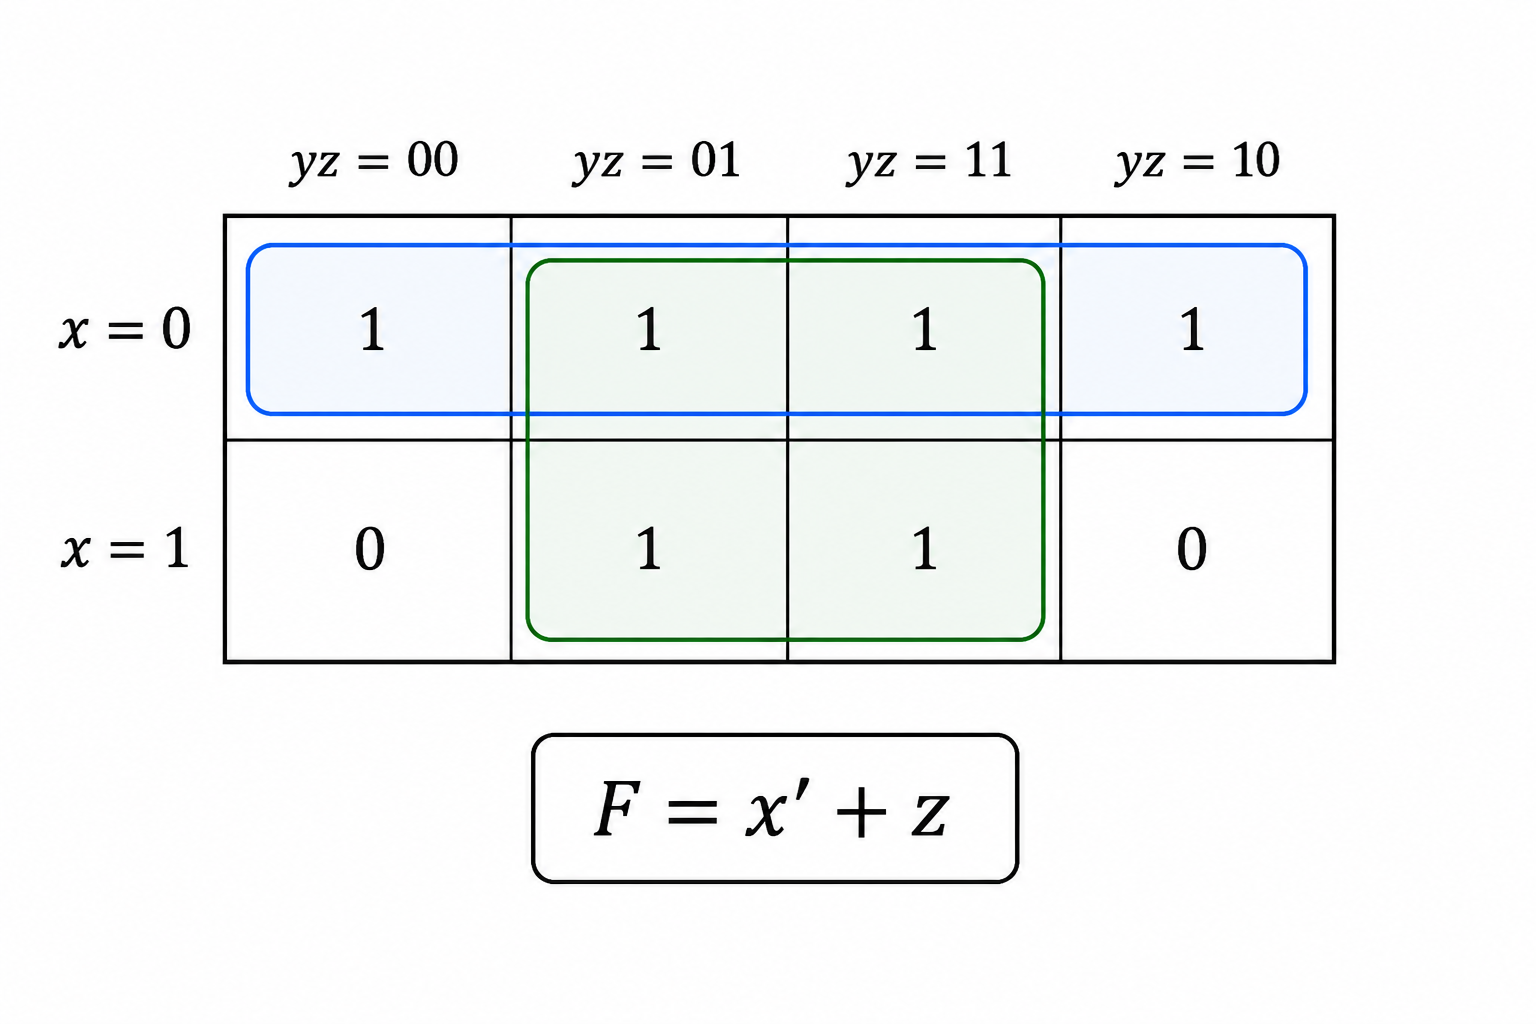
\includegraphics[width=0.82\textwidth]{Figures/png_ready/kmap-grouping-generated.png}
    \caption{การจัดกลุ่มใน K-map}
    \label{fig:kmap-grouping}
\end{figure}

\begin{ex}[การลดรูปด้วยแผนที่คาร์นอ 4 ตัวแปร]
\label{ex:kmap-4var}
ใช้ K-map ลดรูป $f(w, x, y, z) = \sum(0, 1, 2, 3, 4, 6, 8, 9, 12, 14)$

\begin{center}
\begin{tabular}{|c|c|c|c|c|}
\hline
 & $yz = 00$ & $yz = 01$ & $yz = 11$ & $yz = 10$ \\
\hline
$wx = 00$ & 1 & 1 & 1 & 1 \\
\hline
$wx = 01$ & 1 & 0 & 0 & 1 \\
\hline
$wx = 11$ & 1 & 0 & 0 & 1 \\
\hline
$wx = 10$ & 1 & 1 & 0 & 0 \\
\hline
\end{tabular}
\end{center}
\end{ex}
\begin{solution}
\begin{align*}
\{m_0, m_1, m_2, m_3\}\ (\text{แถว } wx = 00) &\Rightarrow w'x'\\
\{m_4, m_6, m_{12}, m_{14}\}\ (\text{แถว } wx = 01 \text{ กับ } wx = 11,\ z = 0) &\Rightarrow xz'\\
\{m_0, m_1, m_8, m_9\}\ (\text{แถวบนสุดกับล่างสุด วนขอบ},\ y = 0) &\Rightarrow x'y'
\end{align*}
$\therefore f = w'x' + xz' + x'y'$ \solhere
\end{solution}

กลุ่ม $\{m_0, m_1, m_8, m_9\}$ ในตัวอย่างข้างต้นเกิดจากการวนขอบในแนวตั้ง คือแถวบนสุดติดกับแถวล่างสุด แผนที่ 4 ตัวแปรวนขอบได้ทั้งสองแนวพร้อมกัน จึงเกิดกรณีพิเศษที่ช่องมุมทั้งสี่รวมเป็นกลุ่มเดียวได้ ทั้งที่มองด้วยตาแล้วดูเหมือนอยู่ห่างกันที่สุดในตาราง

\begin{ex}[การจับกลุ่มวนขอบที่มุมทั้งสี่]
\label{ex:kmap-corner-wrap}
จงใช้แผนที่คาร์นอลดรูป $f(w, x, y, z) = \sum(0, 2, 8, 10)$

\begin{center}
\begin{tabular}{|c|c|c|c|c|}
\hline
 & $yz = 00$ & $yz = 01$ & $yz = 11$ & $yz = 10$ \\
\hline
$wx = 00$ & 1 & 0 & 0 & 1 \\
\hline
$wx = 01$ & 0 & 0 & 0 & 0 \\
\hline
$wx = 11$ & 0 & 0 & 0 & 0 \\
\hline
$wx = 10$ & 1 & 0 & 0 & 1 \\
\hline
\end{tabular}
\end{center}
\end{ex}
\begin{solution}
ทั้งสี่ช่องที่เป็น 1 อยู่ที่มุมทั้งสี่ของตาราง เมื่อวนขอบในแนวตั้ง แถว $wx = 00$ ติดกับแถว $wx = 10$ และเมื่อวนขอบในแนวนอน คอลัมน์ $yz = 00$ ติดกับคอลัมน์ $yz = 10$ ทั้งสี่ช่องจึงติดกันเป็นกลุ่มสี่เหลี่ยมขนาด 4 ช่องกลุ่มเดียว

ตรวจสอบว่าเป็นกลุ่มที่ถูกต้องได้จากรหัสของทั้งสี่มินเทอม
\begin{align*}
m_0 = 0000, \quad m_2 = 0010, \quad m_8 = 1000, \quad m_{10} = 1010
\end{align*}
ตัวแปร $w$ เปลี่ยนค่าและ $y$ เปลี่ยนค่า จึงตัดทั้งคู่ทิ้ง ส่วน $x = 0$ และ $z = 0$ คงที่ทั้งกลุ่ม จึงเขียนเป็นนิเสธทั้งคู่

$\therefore f(w, x, y, z) = x'z'$ \solhere
\end{solution}

\begin{warning}[การจับกลุ่มวนขอบที่มุมทั้งสี่ในแผนที่คาร์นอ]
กับดักที่พบบ่อยคือมองว่าช่องมุมทั้งสี่แยกกันอยู่ แล้วเขียนเป็นสี่พจน์ที่มีสี่ตัวแปรเต็ม คือ $w'x'y'z' + w'x'yz' + wx'y'z' + wx'yz'$ ซึ่งให้ค่าตรงกับฟังก์ชันเดิมก็จริง แต่ใช้ประตูมากกว่าที่จำเป็นหลายเท่า ทั้งที่คำตอบที่ลดรูปแล้วเหลือเพียงพจน์เดียวสองตัวแปร ให้ยึดหลักว่าเซลล์ติดกันคือเซลล์ที่รหัสต่างกันหนึ่งบิต ไม่ใช่เซลล์ที่วาดอยู่ติดกันบนกระดาษ
\end{warning}

\subsection{ค่าไม่สนใจในแผนที่คาร์นอ (Don't Care Conditions)}
\label{sec:dont-care}
ในงานออกแบบระบบดิจิทัลจริง ชุดข้อมูลขาเข้าบางชุดอาจไม่มีทางเกิดขึ้นได้ตามข้อกำหนดการทำงานของระบบ (เช่น เลขฐานสองที่มีค่าเกิน 9 ในระบบเลข BCD) หรือเป็นกรณีที่สัญญาณขาออกไม่มีผลต่อการทำงาน สภาวะดังกล่าวเรียกว่า \textbf{สภาวะไม่สนใจ (Don't Care Conditions)} ซึ่งเขียนแทนด้วยสัญลักษณ์ $d$ หรือ $X$ ในแผนที่คาร์นอ ผู้ออกแบบมีอิสระที่จะกำหนดให้ค่า $d$ เป็น 1 (หากช่วยขยายกลุ่มให้ใหญ่ขึ้นเพื่อลดรูปตัวแปร) หรือกำหนดให้เป็น 0 (หากไม่ต้องการนำมารวมกลุ่ม) เพื่อให้ได้วงจรที่เรียบง่ายและประหยัดที่สุด~\parencite{mano2018digital}

\begin{principle}[การใช้ค่าไม่สนใจในการจับกลุ่ม]
\label{prin:dont-care}
\index{ค่าไม่สนใจ}
เขียนสัญลักษณ์ $d$ ลงในช่องที่เป็นค่าไม่สนใจ แล้วปฏิบัติกับช่องเหล่านั้นตามกฎต่อไปนี้

\begin{enumerate}
    \item ช่อง $d$ \textbf{รวมเข้ากลุ่มได้} เสมือนเป็น 1 ถ้าการรวมนั้นทำให้กลุ่มที่จำเป็นอยู่แล้วขยายใหญ่ขึ้น
    \item ช่อง $d$ \textbf{ไม่ใช่ช่องที่ต้องถูกคลุม} ต่างจากช่องที่เป็น 1 ตามกฎข้อ 5 ใน~\autoref{prin:kmap-rules}
    \item จึง \textbf{ห้ามสร้างกลุ่มขึ้นมาเพื่อคลุมช่อง $d$ โดยเฉพาะ} เพราะจะได้พจน์เพิ่มโดยไม่ได้ประโยชน์
\end{enumerate}

สรุปเป็นเกณฑ์เดียวได้ว่า ตั้ง $d$ เป็น 1 เมื่อมันช่วยขยายกลุ่มที่ต้องมีอยู่แล้ว และตั้งเป็น 0 ในกรณีอื่นทั้งหมด ข้อผิดพลาดที่พบบ่อยคือเข้าใจว่าต้องตั้ง $d$ ทุกช่องเป็น 1 ซึ่งมักทำให้ได้นิพจน์ที่ยาวกว่าเดิม
\end{principle}

\begin{ex}[การลดรูปด้วยค่าไม่สนใจในวงจรตรวจเลขรหัสบีซีดี]
\label{ex:kmap-dont-care}
วงจรหนึ่งรับเลขรหัสบีซีดี (BCD) ขนาด 4 บิต $wxyz$ ซึ่งใช้แทนเลขโดดฐานสิบ 0 ถึง 9 เท่านั้น รหัส 1010 ถึง 1111 จึงไม่มีทางเกิดขึ้น จงออกแบบฟังก์ชัน $f$ ที่ให้ผลลัพธ์เป็น 1 เมื่อเลขโดดที่รับเข้ามามีค่าตั้งแต่ 5 ขึ้นไป นั่นคือ $f = \sum m(5, 6, 7, 8, 9) + d(10, 11, 12, 13, 14, 15)$

\begin{center}
\begin{tabular}{|c|c|c|c|c|}
\hline
 & $yz = 00$ & $yz = 01$ & $yz = 11$ & $yz = 10$ \\
\hline
$wx = 00$ & 0 & 0 & 0 & 0 \\
\hline
$wx = 01$ & 0 & 1 & 1 & 1 \\
\hline
$wx = 11$ & $d$ & $d$ & $d$ & $d$ \\
\hline
$wx = 10$ & 1 & 1 & $d$ & $d$ \\
\hline
\end{tabular}
\end{center}
\end{ex}
\begin{solution}
จับกลุ่มโดยดึงช่อง $d$ เข้ามาช่วยขยายกลุ่ม
\begin{align*}
\{m_8, m_9, m_{10}, m_{11}, m_{12}, m_{13}, m_{14}, m_{15}\}\ (\text{สองแถวล่าง},\ w = 1) &\Rightarrow w\\
\{m_5, m_7, m_{13}, m_{15}\}\ (\text{คอลัมน์ } yz = 01, 11 \text{ ที่ } x = 1) &\Rightarrow xz\\
\{m_6, m_7, m_{14}, m_{15}\}\ (\text{คอลัมน์ } yz = 11, 10 \text{ ที่ } x = 1) &\Rightarrow xy
\end{align*}
ทั้งสามกลุ่มคลุมช่องที่เป็น 1 ครบทั้ง $m_5, m_6, m_7, m_8, m_9$ แล้ว

$\therefore f(w, x, y, z) = w + xy + xz$ \solhere

เปรียบเทียบกับกรณีที่ไม่ใช้ค่าไม่สนใจ คือบังคับให้ช่อง $d$ ทุกช่องเป็น 0 จะจับกลุ่มได้เพียงกลุ่มละ 2 ช่อง ได้ผลลัพธ์เป็น $w x' y' + w' x z + w' x y$ ซึ่งถูกต้องเช่นกันแต่ใช้ตัวแปรรวม 9 ตัวเทียบกับ 5 ตัว การใช้ค่าไม่สนใจจึงลดขนาดวงจรลงได้อย่างมีนัยสำคัญ
\end{solution}

\section{การประยุกต์ในวงจรดิจิทัล}
\label{sec:boolean-applications}

พีชคณิตบูลีนเป็นรากฐานทางทฤษฎีของการออกแบบวงจรดิจิทัล ทุกกระบวนการประมวลผลและการคำนวณในระบบคอมพิวเตอร์สมัยใหม่ ล้วนถูกแปลงเป็นการดำเนินการทางตรรกศาสตร์บนสัญญาณไฟฟ้า 2 ระดับ ($0$ และ $1$) การเข้าใจความสัมพันธ์ระหว่างนิพจน์บูลีนกับโครงสร้างวงจรฮาร์ดแวร์จริง จึงเป็นทักษะที่จำเป็นในการทำความเข้าใจสถาปัตยกรรมคอมพิวเตอร์ กระบวนการออกแบบวงจรดิจิทัลจะเริ่มต้นจากการวิเคราะห์ข้อกำหนดของระบบ แปลงเป็นฟังก์ชันบูลีน ดำเนินการลดรูปนิพจน์ให้กะทัดรัดที่สุด และสังเคราะห์ออกมาเป็นวงจรที่ประกอบด้วยลอจิกเกต (Logic Gates)~\parencite{gersting2014structures}

\subsection{ประตูตรรกะ (Logic Gates)}
ลอจิกเกต (Logic Gates) เป็นอุปกรณ์อิเล็กทรอนิกส์พื้นฐานที่ทำหน้าที่ประมวลผลสัญญาณตามการดำเนินการบูลีนในระดับฮาร์ดแวร์ โดยรับระดับแรงดันไฟฟ้าที่แทนค่า $0$ และ $1$ ทางช่องสัญญาณขาเข้า และส่งสัญญาณผลลัพธ์ขาออกตามตารางค่าความจริงของฟังก์ชันนั้น ๆ การแปลงนิพจน์บูลีนเป็นวงจรจริงสามารถทำได้โดยแทนตัวดำเนินการแต่ละตัวด้วยลอจิกเกตที่สอดคล้องกัน โดยลอจิกเกตพื้นฐานที่สำคัญมีดังนี้~\parencite{wakerly2018digital}


\begin{definition}[ประเภทของประตูตรรกะ]
\index{ประตูตรรกะ!ประเภท}
ประเภทของประตูตรรกะพื้นฐาน ได้แก่
\begin{enumerate}
    \item NOT Gate (Inverter) แสดงผล $a'$
    \item AND Gate แสดงผล $a \cdot b$
    \item OR Gate แสดงผล $a + b$
    \item NAND Gate แสดงผล $(a \cdot b)'$
    \item NOR Gate แสดงผล $(a + b)'$
    \item XOR Gate แสดงผล $a \oplus b = a b' + a' b$
    \item XNOR Gate แสดงผล $(a \oplus b)' = a b + a' b'$
\end{enumerate}
\end{definition}

\begin{principle}[NAND Gate ในฐานะเกตสากล (Universal Gate)]
\index{ประตูตรรกะ!NAND Gate}
\textbf{NAND Gate} เป็นเกตสากล (Universal Gate) เนื่องจากสามารถนำมาต่อเชื่อมเพื่อสร้างเกตตรรกะพื้นฐานอื่น ๆ ได้ทั้งหมด โดย NAND Gate ให้ผลลัพธ์การทำงานคือ $Y = (a \cdot b)' = \overline{a \cdot b}$

ค่าผลลัพธ์ในทุกกรณีของสัญญาณอินพุต $(a, b)$ แสดงไว้ในตารางที่~\ref{tab:nand-nor-truth} จุดที่ควรสังเกตคือ NAND ให้ผลเป็น 0 เพียงกรณีเดียว คือเมื่ออินพุตทั้งสองเป็น 1 ซึ่งตรงข้ามกับ AND ทุกแถวพอดี

การสร้างประตูตรรกะพื้นฐานจากประตู NAND เพียงอย่างเดียวทำได้ดังนี้
\begin{enumerate}[label=\textbf{\arabic*.},leftmargin=1.5em,itemsep=0.4em]
    \item \textbf{การสร้างประตู NOT จาก NAND} เมื่อป้อนสัญญาณเข้าเดียวกันทั้งสองช่อง $(a, a)$ จะได้
    \[ a' = (a \cdot a)' \]
    \item \textbf{การสร้าง AND Gate จาก NAND:} นำผลลัพธ์ของ NAND Gate มาผ่าน NOT Gate (NAND ที่ป้อนอินพุตซ้ำ) ได้ว่า
    \[ a \cdot b = ((a \cdot b)')' \]
    \item \textbf{การสร้างประตู OR จาก NAND} ใช้กฎเดอมอร์แกนร่วมกับการนิเสธสัญญาณเข้าแต่ละตัว
    \[ a + b = (a' \cdot b')' = ((a \cdot a)' \cdot (b \cdot b)')' \]
\end{enumerate}
\end{principle}

\begin{principle}[NOR Gate ในฐานะเกตสากล (Universal Gate)]
\index{ประตูตรรกะ!NOR Gate}
\textbf{NOR Gate} เป็นเกตสากล (Universal Gate) เช่นเดียวกับ NAND Gate เนื่องจากสามารถนำมาต่อเพื่อสร้างเกตตรรกะอื่น ๆ ได้ทั้งหมด โดย NOR Gate ให้ผลลัพธ์การทำงานคือ $Y = (a + b)'$

ค่าผลลัพธ์ในทุกกรณีแสดงไว้ในตารางที่~\ref{tab:nand-nor-truth} เช่นเดียวกัน โดย NOR ให้ผลเป็น 1 เพียงกรณีเดียว คือเมื่ออินพุตทั้งสองเป็น 0 ซึ่งตรงข้ามกับ OR ทุกแถวพอดี

การสร้างประตูตรรกะพื้นฐานจากประตู NOR เพียงอย่างเดียวทำได้ดังนี้
\begin{enumerate}[label=\textbf{\arabic*.},leftmargin=1.5em,itemsep=0.4em]
    \item \textbf{การสร้างประตู NOT จาก NOR} เมื่อป้อนสัญญาณเข้าเดียวกันทั้งสองช่อง $(a, a)$ จะได้
    \[ a' = (a + a)' \]
    \item \textbf{การสร้าง OR Gate จาก NOR:} นำผลลัพธ์ของ NOR Gate มาผ่าน NOT Gate (NOR ที่ป้อนอินพุตซ้ำ) ได้ว่า
    \[ a + b = ((a + b)')' \]
    \item \textbf{การสร้างประตู AND จาก NOR} ใช้กฎเดอมอร์แกนร่วมกับการนิเสธสัญญาณเข้าแต่ละตัว
    \[ a \cdot b = (a' + b')' = ((a + a)' + (b + b)')' \]
\end{enumerate}
\end{principle}

\begin{table}[H]
    \centering
    \caption{ตารางค่าความจริงของ NAND และ NOR เทียบกับ AND และ OR}
    \label{tab:nand-nor-truth}
    \begin{tabular}{|c|c|c|c|c|c|}
        \hline
        $a$ & $b$ & $a \cdot b$ & $(a \cdot b)'$ (NAND) & $a + b$ & $(a + b)'$ (NOR) \\ \hline
        0 & 0 & 0 & 1 & 0 & 1 \\ \hline
        0 & 1 & 0 & 1 & 1 & 0 \\ \hline
        1 & 0 & 0 & 1 & 1 & 0 \\ \hline
        1 & 1 & 1 & 0 & 1 & 0 \\ \hline
    \end{tabular}
\end{table}

ตารางที่~\ref{tab:nand-nor-truth} วางคอลัมน์ของ AND และ OR ไว้ข้างคอลัมน์ของ NAND และ NOR เพื่อให้เห็นว่าเกตทั้งสองคู่ให้ผลตรงข้ามกันทุกแถว เหตุที่เกตทั้งสองสร้างเกตอื่นได้ทั้งหมดก็เพราะรวมการนิเสธไว้ในตัวเองแล้ว จึงไม่ต้องอาศัย NOT Gate แยกต่างหาก ส่วนสัญลักษณ์และการต่อวงจรของเกตสากลทั้งสองแสดงในรูปที่~\ref{fig:universal-gates}

\begin{figure}[H]
    \centering
    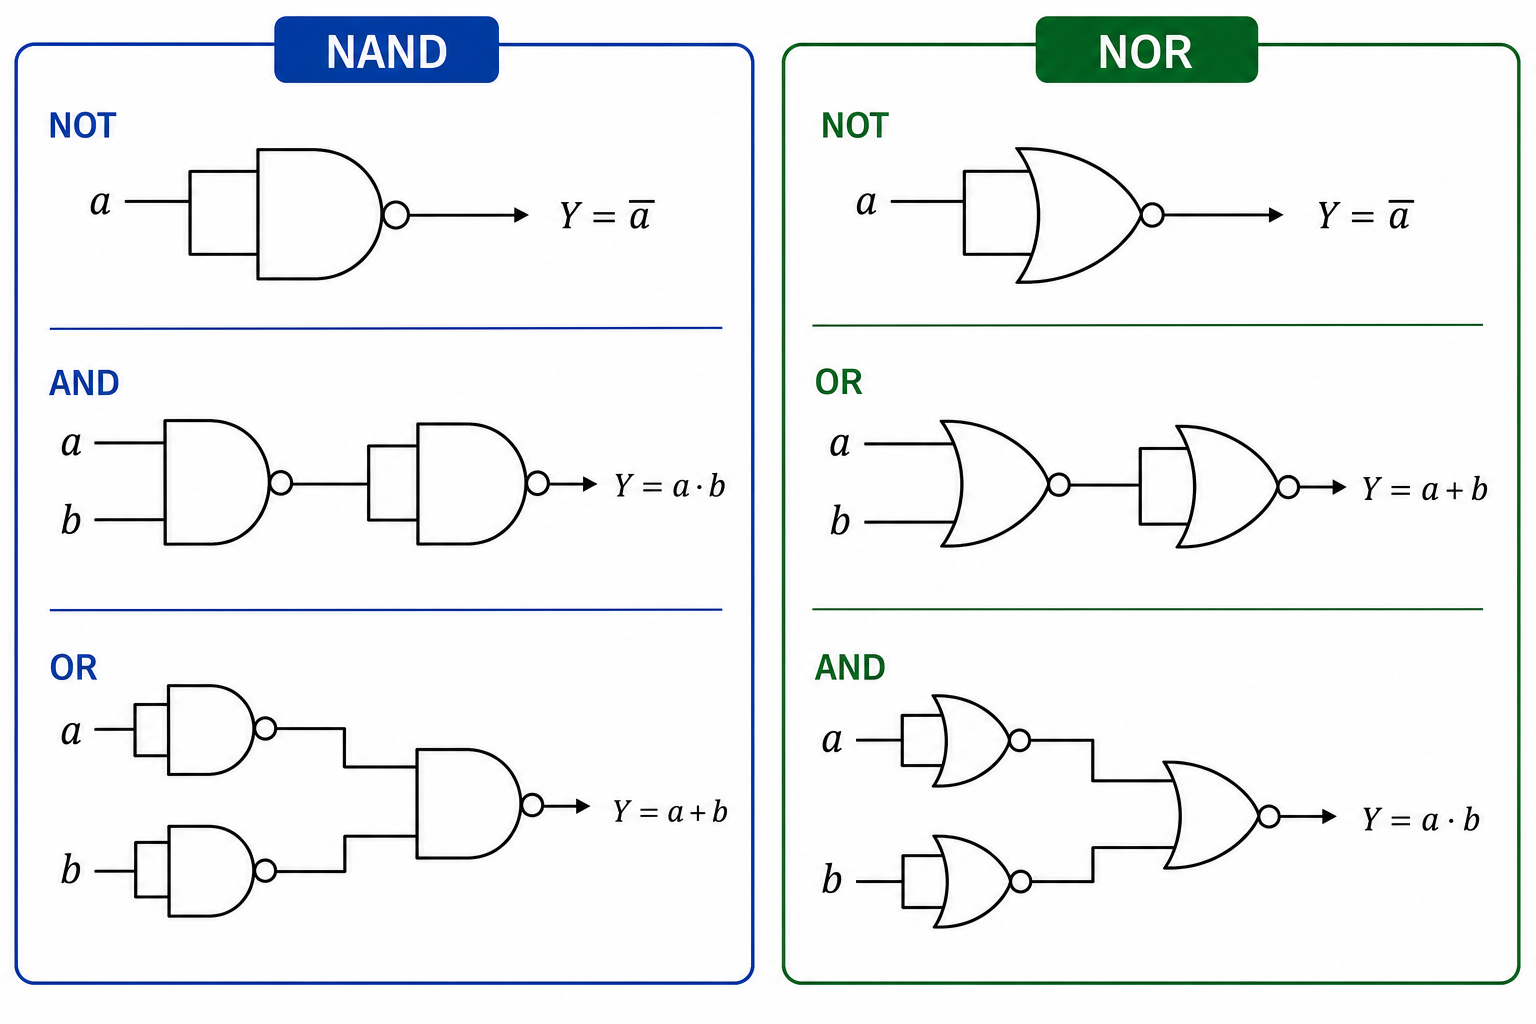
\includegraphics[width=0.82\textwidth]{Figures/png_ready/universal-gates-generated.png}
    \caption{เกตสากล NAND และ NOR}
    \label{fig:universal-gates}
\end{figure}

\begin{ex}[การวาดวงจรจากนิพจน์บูลีน]
\label{ex:draw-circuit}
จงอธิบายลำดับการต่อประตูตรรกะเพื่อสร้างวงจรของ $f(x, y, z) = x y + x' z$ พร้อมนับจำนวนประตูแต่ละชนิดที่ใช้
\end{ex}
\begin{solution}
\begin{align*}
x &\xrightarrow{\text{NOT}} x'\\
(x, y) &\xrightarrow{\text{AND}} xy, \qquad (x', z) \xrightarrow{\text{AND}} x'z\\
(xy, x'z) &\xrightarrow{\text{OR}} xy + x'z = f
\end{align*}

$\therefore$ วงจรใช้ประตู NOT 1 ตัว ประตู AND 2 ตัว และประตู OR 1 ตัว \solhere
\end{solution}

\begin{ex}[การลดรูปก่อนวาดวงจร]
\label{ex:simplify-then-draw}
ลดรูปและวาดวงจรสำหรับ $f(a, b, c) = (a + b) \cdot (a + c)$
\end{ex}
\begin{solution}
\begin{align*}
f &= (a + b)(a + c)\\
&= a + bc \quad \text{(Distributive)}
\end{align*}
วงจร $(b,c) \xrightarrow{\text{AND}} bc$ แล้ว $(a, bc) \xrightarrow{\text{OR}} a + bc$ ใช้ประตู AND 1 ตัวกับประตู OR 1 ตัว จากเดิมที่ต้องใช้ประตู OR 2 ตัวกับประตู AND 1 ตัว

$\therefore$ การลดรูปช่วยลดจำนวนประตูจาก 3 ตัวเหลือ 2 ตัว \solhere
\end{solution}

\subsection{การออกแบบวงจรเชิงผสม (Combinational Circuit)}
วงจรเชิงผสม (Combinational Logic Circuits) คือ วงจรดิจิทัลที่สัญญาณขาออกขึ้นอยู่กับค่าของสัญญาณขาเข้า ณ ขณะเวลาปัจจุบันเท่านั้น โดยไม่มีหน่วยความจำและไม่ขึ้นกับสถานะในอดีต การออกแบบวงจรเชิงผสมประกอบด้วยขั้นตอนการแปลงข้อกำหนดของระบบเป็นตารางค่าความจริง การเขียนฟังก์ชันบูลีนในรูปแบบบัญญัติ การลดรูปนิพจน์ด้วยแผนที่คาร์นอ และการต่อวงจรด้วยลอจิกเกตตามลำดับ~\parencite{wakerly2018digital}

\begin{ex}[การออกแบบวงจรตรวจสอบจำนวนคู่]
\label{ex:even-detector}
ออกแบบวงจรที่ตรวจสอบว่าจำนวน 3-bit เป็นเลขคู่ (even)
\end{ex}
\begin{solution}
ให้บิต $z$ เป็นบิตต่ำสุด (LSB); จำนวนเป็นเลขคู่ ก็ต่อเมื่อ $z = 0$ ได้ minterms $m_0, m_2, m_4, m_6$
\begin{align*}
f(x, y, z) &= x'y'z' + x'yz' + xy'z' + xyz'\\
&= z' \quad (\text{ตรวจสอบบิตต่ำสุด})
\end{align*}

$\therefore$ วงจรตรวจสอบจำนวนคู่ใช้เพียงประตู NOT ตัวเดียวที่บิตต่ำสุด เพราะจำนวนคู่คือจำนวนที่บิตต่ำสุดเป็น 0 \solhere
\end{solution}

\subsection{การสร้างวงจรสองระดับ (Two-level Realization)}
\label{sec:two-level}
การสร้างวงจรดิจิทัลแบบ 2 ระดับ (Two-Level Realization) เป็นการจัดวางลอจิกเกตหลักเพียง 2 ชั้นก่อนส่งสัญญาณถึงขาออก (ไม่นับอินเวอร์เตอร์ที่ใช้กลับค่าสัญญาณตัวแปร) นิพจน์ในรูปแบบ SOP และ POS สามารถแปลงเป็นวงจร 2 ระดับได้โดยตรง โครงสร้างนี้มีจุดเด่นด้านความเร็วในการทำงาน เนื่องจากสัญญาณจะผ่านเกตเพียง 2 ชั้น ทำให้มีเวลาหน่วงการแพร่สัญญาณที่ต่ำและคงที่~\parencite{wakerly2018digital}

\begin{principle}[การสร้างวงจรสองระดับ]
\textbf{Two-level Realization:}
\begin{enumerate}
    \item SOP (Sum of Products) AND gates ระดับแรก แล้ว OR gate ระดับที่สอง
    \item POS (Product of Sums) OR gates ระดับแรก แล้ว AND gate ระดับที่สอง
\end{enumerate}
\end{principle}

\begin{ex}[การสร้างวงจรสองระดับแบบ SOP]
\label{ex:two-level-sop}
จงอธิบายการสร้างวงจรสองระดับแบบ SOP ของ $f(x, y, z) = y' + x y + x' y' z$ พร้อมระบุว่าความหน่วงเวลาของวงจรขึ้นกับสิ่งใด
\end{ex}
\begin{solution}
ระดับแรก $(x,y) \xrightarrow{\text{AND}} xy$ และ $(x',y',z) \xrightarrow{\text{AND}} x'y'z$ (ใช้ NOT สร้าง $x', y'$); ระดับที่สอง $(y',\ xy,\ x'y'z) \xrightarrow{\text{OR}} f$

$\therefore$ วงจรสองระดับนี้มีความหน่วงเวลาคงที่ ไม่ขึ้นกับจำนวนพจน์ เพราะทุกสัญญาณผ่านประตูเพียงสองชั้น \solhere
\end{solution}

\subsection{วงจรบวกครึ่งและวงจรบวกเต็ม (Half Adder and Full Adder)}
\label{sec:adders}
วงจรบวกเลขฐานสอง (Binary Adders) เป็นตัวอย่างคลาสสิกของการนำพีชคณิตบูลีนไปสร้างเป็นวงจรคำนวณในหน่วยประมวลผลกลาง โดย \textbf{วงจรบวกครึ่ง (Half Adder)} รับข้อมูลขาเข้า 2 บิตเพื่อคำนวณผลบวก ($S$) และบิตทด ($C$) ในขณะที่ \textbf{วงจรบวกเต็ม (Full Adder)} รับสัญญาณขาเข้า 3 บิต ซึ่งรวมบิตทดรับเข้า ($C_{in}$) จากหลักก่อนหน้า ทำให้สามารถนำวงจรบวกเต็มมาต่ออนุกรมกันเป็นชุดเพื่อบวกเลขฐานสองขนาดหลายบิต (Multi-bit Adder) ภายในหน่วยคำนวณและตรรกะ (ALU) ได้อย่างสมบูรณ์~\parencite{wakerly2018digital}

\begin{ex}[การออกแบบวงจรบวกครึ่ง]
\label{ex:half-adder}
ออกแบบวงจรบวกครึ่ง (Half Adder)
\end{ex}
\begin{solution}
Half Adder รับ 2 บิต $x, y$
\begin{align*}
S &= x \oplus y = x y' + x' y\\
C &= x \cdot y
\end{align*}

$\therefore$ วงจรบวกครึ่งใช้ประตู XOR 1 ตัวสำหรับผลบวก และประตู AND 1 ตัวสำหรับตัวทด \solhere
\end{solution}

\begin{ex}[การออกแบบวงจรบวกเต็ม]
\label{ex:full-adder}
ออกแบบ Full Adder
\end{ex}
\begin{solution}
Full Adder รับ 3 บิต $x, y, z_{in}$
\begin{align*}
S &= x \oplus y \oplus z_{in}\\
C_{out} &= x y + x z_{in} + y z_{in}
\end{align*}

$\therefore$ วงจรบวกเต็มต่างจากวงจรบวกครึ่งตรงที่รับตัวทดเข้ามาด้วย จึงนำไปต่อกันเป็นชุดสำหรับเลขหลายบิตได้ \solhere
\end{solution}

\subsection{สมมูลของพีชคณิตบูลีน (Boolean Algebra Equivalence)}
\label{sec:boolean-equivalence}
กฎที่ศึกษามาตลอดบทนี้มีจำนวนมากจนจดจำได้ยาก การรวบรวมไว้ในที่เดียวช่วยให้เปรียบเทียบและเลือกใช้ได้สะดวกขณะลดรูปนิพจน์ ตารางต่อไปนี้สรุปกฎทั้งหมดพร้อมชื่อเรียกมาตรฐาน โดยจัดคู่กฎที่เป็นคู่ทวิภาค (Dual) ไว้ในแถวเดียวกัน ซึ่งได้จากการสลับ AND กับ OR และสลับ 0 กับ 1 พร้อมกัน~\parencite{mano2018digital}

ตารางที่~\ref{tab:boolean-op-summary} สรุปเงื่อนไขที่ทำให้การดำเนินการพื้นฐานแต่ละตัวให้ผลลัพธ์เป็น 1 หรือ 0 และตารางที่~\ref{tab:boolean-identities} สรุปกฎทั้งหมดโดยจัดคู่ทวิภาคไว้ในแถวเดียวกัน

\begin{table}[!htb]
\centering
\caption{เงื่อนไขที่ทำให้การดำเนินการพื้นฐานให้ผลลัพธ์เป็น 1 และ 0}
\label{tab:boolean-op-summary}
\begin{tabular}{|c|c|c|c|}
\hline
การดำเนินการ & สัญลักษณ์ & ผลลัพธ์เป็น 1 เมื่อ & ผลลัพธ์เป็น 0 เมื่อ \\
\hline
OR & $+$ & มีอินพุตอย่างน้อยหนึ่งตัวเป็น 1 & อินพุตทุกตัวเป็น 0 \\
\hline
AND & $\cdot$ & อินพุตทุกตัวเป็น 1 & มีอินพุตอย่างน้อยหนึ่งตัวเป็น 0 \\
\hline
NOT & $'$ & อินพุตเป็น 0 & อินพุตเป็น 1 \\
\hline
\end{tabular}
\end{table}

\begin{table}[!htb]
\centering
\caption{สรุปกฎของพีชคณิตบูลีน โดยกฎในแถวเดียวกันเป็นคู่ทวิภาคของกันและกัน}
\label{tab:boolean-identities}
\begin{tabular}{|c|c|c|}
\hline
กฎทางพีชคณิต & รูปแบบ OR & รูปแบบ AND \\
\hline
กฎเอกลักษณ์ (Identity) & $x + 0 = x$ & $x \cdot 1 = x$ \\
\hline
กฎครอบงำ (Domination) & $x + 1 = 1$ & $x \cdot 0 = 0$ \\
\hline
กฎนิจพล (Idempotent) & $x + x = x$ & $x \cdot x = x$ \\
\hline
กฎคอมพลีเมนต์ (Complement) & $x + x' = 1$ & $x \cdot x' = 0$ \\
\hline
กฎการสลับที่ (Commutative) & $x + y = y + x$ & $x \cdot y = y \cdot x$ \\
\hline
กฎการเปลี่ยนหมู่ (Associative) & $(x + y) + z = x + (y + z)$ & $(x \cdot y) \cdot z = x \cdot (y \cdot z)$ \\
\hline
กฎการแจกแจง (Distributive) & $x + yz = (x + y)(x + z)$ & $x(y + z) = xy + xz$ \\
\hline
กฎการดูดกลืน (Absorption) & $x + xy = x$ & $x(x + y) = x$ \\
\hline
กฎเดอมอร์แกน (De Morgan's) & $(x + y)' = x' y'$ & $(xy)' = x' + y'$ \\
\hline
\end{tabular}
\end{table}

\section{ตัวอย่างในวิทยาการคอมพิวเตอร์}
\label{sec:computer-science-examples}

พีชคณิตบูลีนมีการประยุกต์ใช้อย่างกว้างขวางในวิทยาการคอมพิวเตอร์ นอกเหนือจากการออกแบบวงจรดิจิทัลแล้ว หลักการทางบูลีนยังปรากฏอย่างเด่นชัดในโครงสร้างการตัดสินใจของภาษาโปรแกรม การเขียนคำสั่งสืบค้นในระบบฐานข้อมูล ขั้นตอนวิธีการเข้ารหัสลับ และการออกแบบสถาปัตยกรรมระบบคอมพิวเตอร์ การศึกษาตัวอย่างการประยุกต์ใช้งานเหล่านี้จะช่วยให้ผู้เรียนเชื่อมโยงความรู้เชิงทฤษฎีเข้ากับการปฏิบัติการทางวิศวกรรมคอมพิวเตอร์ได้อย่างเป็นรูปธรรม~\parencite{gersting2014structures}

\subsection{การใช้แผนที่คาร์นอในงานออกแบบจริง}
หัวข้อย่อยนี้นำเทคนิคแผนที่คาร์นอที่ได้ศึกษามาประยุกต์ใช้กับโจทย์การออกแบบวงจรจริง ซึ่งช่วยให้สามารถลดทอนความซับซ้อนของวงจรได้อย่างมีประสิทธิภาพก่อนการประกอบวงจรฮาร์ดแวร์~\parencite{roth2021logic}

\begin{ex}[การใช้แผนที่คาร์นอในงานออกแบบจริง]
\label{ex:kmap-real-design}
ลดรูปฟังก์ชันบูลีน $F(x,y,z) = \sum(0,1,2,3,5,7)$ โดยใช้ K-map

K-map สำหรับ 3 ตัวแปร ดังนี้


\begin{center}
\begin{tabular}{c|c|c|c|c}
\hline
 & $yz=00$ & $yz=01$ & $yz=11$ & $yz=10$ \\
\hline
$x=0$ & 1 & 1 & 1 & 1 \\
\hline
$x=1$ & 0 & 1 & 1 & 0 \\
\hline
\end{tabular}
\end{center}
\end{ex}
\begin{solution}
\begin{align*}
\{m_0, m_1, m_2, m_3\}\ (\text{แถว } x = 0) &\Rightarrow x'\\
\{m_1, m_3, m_5, m_7\}\ (\text{สองคอลัมน์ } z = 1) &\Rightarrow z
\end{align*}
$\therefore F = x' + z$ \solhere
\end{solution}


\subsection{ตัวอย่างการสร้าง AND จาก NAND}
จากสมบัติของเกตสากล (Universal Gate) ที่ระบุว่าเกต NAND สามารถนำมาต่อเพื่อสร้างการทำงานของลอจิกเกตพื้นฐานอื่น ๆ ได้อย่างสมบูรณ์ ตัวอย่างนี้จะแสดงขั้นตอนการสังเคราะห์เกต AND โดยใช้เกต NAND เพียง 2 ตัว ซึ่งเป็นเทคนิคที่ใช้จริงในสายการผลิตชิปวงจรรวม (Integrated Circuit: IC) เพื่อลดความหลากหลายของชนิดเกตในกระบวนการผลิต~\parencite{mano2018digital}

\begin{ex}[การสร้างประตู AND จากประตู NAND]
\label{ex:and-from-nand}
จงแสดงวิธีสร้างประตู AND ที่ให้ผลลัพธ์ $Y = A \cdot B$ โดยใช้ประตู NAND เพียงชนิดเดียว พร้อมระบุจำนวนประตูที่ใช้
\end{ex}
\begin{solution}
\begin{align*}
\text{NOT จาก NAND}\quad (A \cdot A)' &= A'\\
\text{AND จาก NAND สองตัว}\quad ((AB)')' &= AB
\end{align*}

$\therefore$ สร้างประตู AND ได้ด้วยประตู NAND 2 ตัว คือตัวแรกให้ $(AB)'$ และตัวที่สองทำหน้าที่เป็นตัวนิเสธโดยป้อนสัญญาณเดียวกันเข้าทั้งสองขา ประตู NAND จึงสร้างประตูพื้นฐานได้ทุกชนิด และเรียกว่าประตูสากล \solhere
\end{solution}

\subsection{การต่อวงจรบวกเป็นชุดสำหรับเลขหลายบิต}
วงจรบวกครึ่งและวงจรบวกเต็มสามารถนำมาต่อเรียงกันเป็นวงจรบวกแบบขนาน (Ripple Carry Adder) สำหรับคำนวณเลขฐานสองขนาดหลายบิต โดยส่งบิตทดขาออกจากหลักหนึ่งไปเป็นบิตทดขาเข้าของหลักถัดไป โครงสร้างนี้ทำหน้าที่เป็นแกนหลักในหน่วยคำนวณและตรรกะ (ALU) ของหน่วยประมวลผลกลาง~\parencite{wakerly2018digital} ตัวอย่างต่อไปนี้แสดงการสังเคราะห์วงจรบวกเต็มโดยอาศัยวงจรบวกครึ่ง 2 ชุดร่วมกับเกต OR 1 ตัว ดังแสดงการเปรียบเทียบโครงสร้างในรูปที่~\ref{fig:adders-comparison}

\begin{figure}[H]
    \centering
    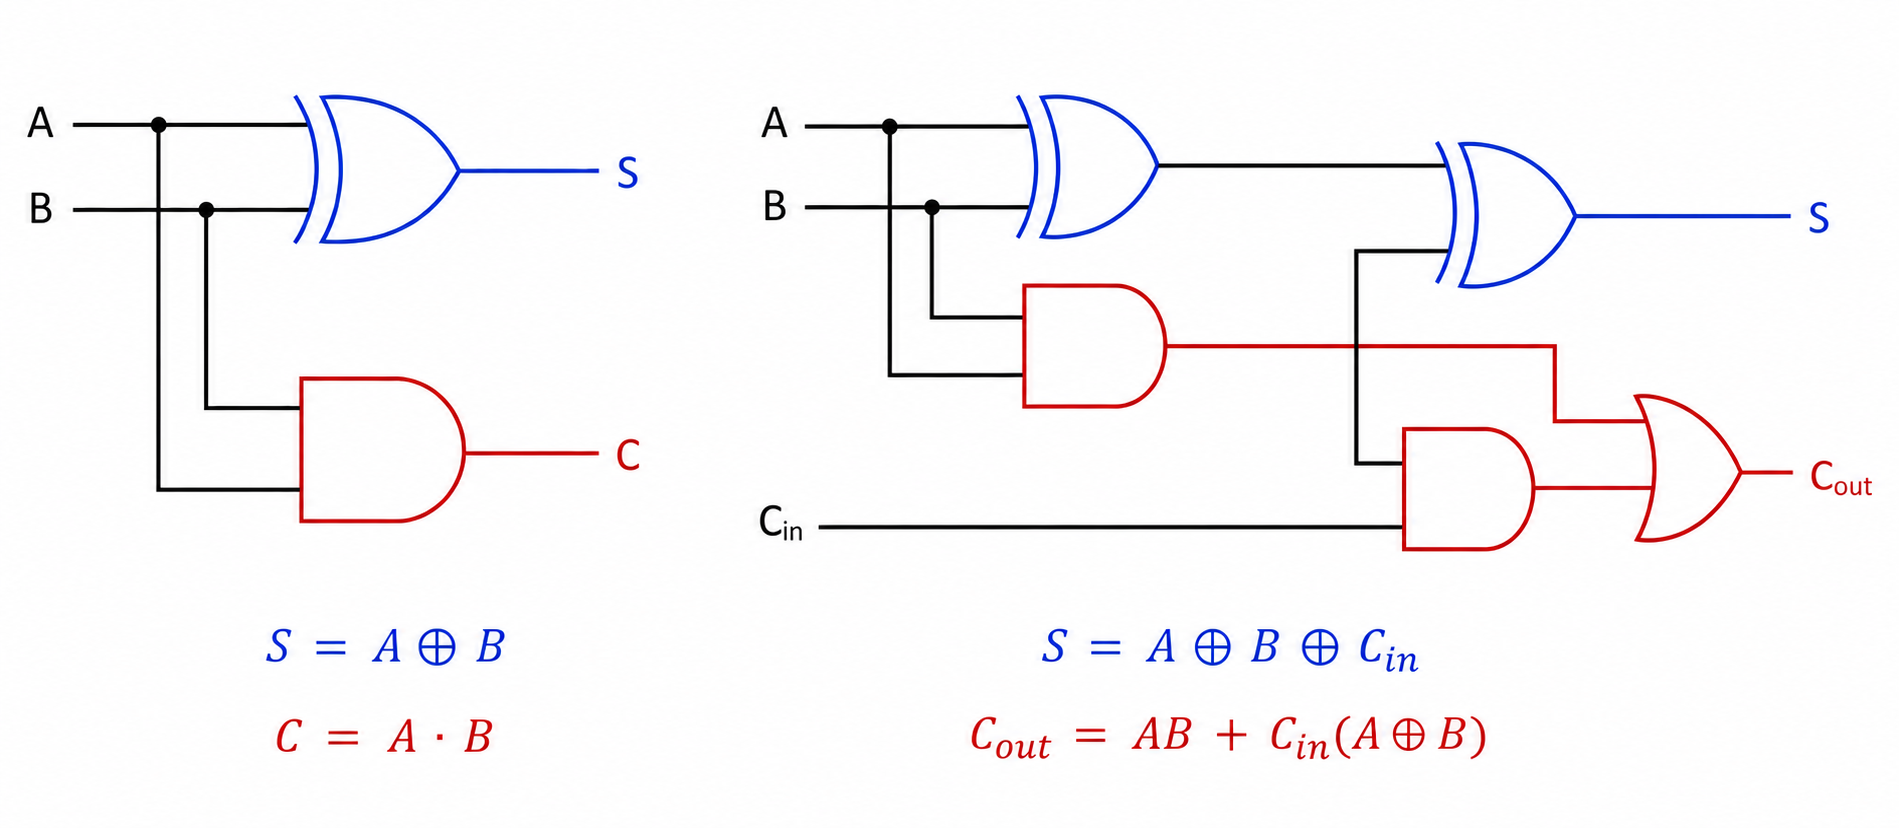
\includegraphics[width=0.82\textwidth]{Figures/png_ready/adders-comparison-generated.png}
    \caption{Half Adder และ Full Adder}
    \label{fig:adders-comparison}
\end{figure}

\begin{ex}[การต่อวงจรบวกครึ่งเป็นวงจรบวกเต็ม]
\label{ex:full-from-half}
Full Adder จาก Half Adders:

$S = A \oplus B \oplus C_{in}$

$C_{out} = AB + C_{in}(A \oplus B)$

สามารถสร้างได้จาก 2 Half Adders + 1 OR gate
\end{ex}
\begin{solution}
\begin{align*}
\text{HA}_1(A, B):\quad S_1 &= A \oplus B, & C_1 &= AB\\
\text{HA}_2(S_1, C_{in}):\quad S &= S_1 \oplus C_{in} = A \oplus B \oplus C_{in}, & C_2 &= C_{in} S_1\\
\text{OR}(C_1, C_2):\quad C_{out} &= AB + C_{in}(A \oplus B)
\end{align*}

$\therefore$ วงจรบวกเต็มหนึ่งตัวสร้างได้จากวงจรบวกครึ่งสองตัวกับประตู OR หนึ่งตัว \solhere
\end{solution}

\subsection{มัลติเพล็กเซอร์และดีมัลติเพล็กเซอร์ (Multiplexer and Demultiplexer)}
\textbf{มัลติเพล็กเซอร์ (Multiplexer: MUX)} และ \textbf{ดีมัลติเพล็กเซอร์ (Demultiplexer: DEMUX)} เป็นวงจรเชิงผสมที่มีบทบาทสำคัญในการควบคุมเส้นทางข้อมูล โดยมัลติเพล็กเซอร์ทำหน้าที่เลือกสัญญาณจากช่องสัญญาณขาเข้าหลายช่อง ($n$ Inputs) ให้ส่งผ่านออกไปยังช่องสัญญาณขาออกเพียงช่องเดียว (1 Output) ตามการควบคุมของสัญญาณเลือก (Select Lines) ในขณะที่ดีมัลติเพล็กเซอร์จะทำหน้าที่ตรงกันข้าม คือ รับสัญญาณขาเข้า 1 ช่องแล้วกระจายไปยังช่องสัญญาณขาออกช่องใดช่องหนึ่งจากหลายช่อง ทั้งสองวงจรสามารถอธิบายการทำงานและออกแบบด้วยนิพจน์บูลีนได้อย่างสมบูรณ์~\parencite{wakerly2018digital}

\begin{definition}[ตัวเลือกข้อมูล (Multiplexer)]
\index{มัลติเพล็กเซอร์!นิยาม}
มัลติเพล็กเซอร์ (Multiplexer: MUX) เป็นวงจรที่เลือก 1 จาก $n$ inputs ไปยัง 1 output โดยใช้ select lines

สำหรับ 4-to-1 MUX:
$$Y = I_0 \cdot S_1' \cdot S_0' + I_1 \cdot S_1' \cdot S_0 + I_2 \cdot S_1 \cdot S_0' + I_3 \cdot S_1 \cdot S_0$$

\begin{center}
\begin{tabular}{|c|c|c|}
\hline
$S_1$ & $S_0$ & สัญญาณออก (Output) \\
\hline
0 & 0 & $I_0$ \\
\hline
0 & 1 & $I_1$ \\
\hline
1 & 0 & $I_2$ \\
\hline
1 & 1 & $I_3$ \\
\hline
\end{tabular}
\end{center}
\end{definition}

\begin{definition}[ตัวกระจายข้อมูล (Demultiplexer)]
\index{ดีมัลติเพล็กเซอร์!นิยาม}
ดีมัลติเพล็กเซอร์ (Demultiplexer: DEMUX) ทำงานตรงข้ามกับ MUX คือรับ 1 input และส่งไปยัง 1 จาก $n$ outputs
\end{definition}

\subsection{การสร้างเครื่องสถานะจำกัดด้วยตรรกะบูลีน (Finite State Machine)}
\textbf{เครื่องสถานะจำกัด (Finite State Machine: FSM)} เป็นแบบจำลองทางคณิตศาสตร์ของวงจรตรรกะเชิงลำดับ (Sequential Circuits) ซึ่งสัญญาณขาออกจะขึ้นอยู่กับทั้งสัญญาณขาเข้าในปัจจุบันและสถานะของวงจรที่ถูกบันทึกไว้ในหน่วยความจำ (ฟลิปฟลอป) การออกแบบ FSM ด้วยพีชคณิตบูลีนทำได้โดยการเข้ารหัสสถานะ (State Encoding) เป็นเลขฐานสอง แล้วสร้างฟังก์ชันบูลีนเพื่อกำหนดสถานะถัดไป (Next State Logic) และสัญญาณขาออก (Output Logic) ตัวอย่างต่อไปนี้แสดงการออกแบบเครื่องสถานะจำกัดแบบมัวร์ (Moore Machine) ซึ่งค่าสัญญาณขาออกจะขึ้นกับสถานะปัจจุบันเท่านั้น~\parencite{wakerly2018digital}

\begin{ex}[การออกแบบเครื่องสถานะจำกัดตรวจจับลำดับบิต]
\label{ex:fsm-sequence}
พิจารณา Moore FSM ที่ตรวจสอบลำดับบิต ``10'' โดย output เป็น 1 หลังจากอ่านบิต 0 ที่ต่อจากบิต 1 แล้ว ดังนี้


\begin{center}
\begin{tabular}{|c|c|c|c|}
\hline
สถานะปัจจุบัน (State) & สัญญาณเข้า=0 & สัญญาณเข้า=1 & สัญญาณออก (Output) \\
\hline
S0 (เริ่มต้น) & S0 & S1 & 0 \\
\hline
S1 (พบบิต 1) & S2 & S1 & 0 \\
\hline
S2 (พบลำดับ 10) & S0 & S1 & 1 \\
\hline
\end{tabular}
\end{center}

กำหนด state encoding: S0=00, S1=01, S2=10 โดยกำหนดสถานะ 11 เป็นค่าไม่สนใจ

จากตารางสถานะ จะได้สมการสถานะถัดไปและผลลัพธ์ดังนี้
\[
Q_1^+ = Q_0X', \qquad Q_0^+ = X, \qquad Y = Q_1Q_0'
\]

ตัวอย่างเช่น input $11010$ จะเดินสถานะเป็น $S0 \rightarrow S1 \rightarrow S1 \rightarrow S2 \rightarrow S1 \rightarrow S2$ ดังนั้น output หลังอ่านแต่ละบิตคือ $0,0,1,0,1$ โดยค่า 1 เกิดเมื่อเครื่องเข้าสู่ state $S2$
\end{ex}
\begin{solution}
ใช้ตัวแปรสถานะ $Q_1,Q_0$ แทนสามสถานะ จะได้ $Q_1^+=Q_0X'$, $Q_0^+=X$ และ $Y=Q_1Q_0'$ ซึ่งเป็นสมการสำหรับสร้างวงจรสถานะถัดไปและวงจรผลลัพธ์

$\therefore$ เครื่องสถานะจำกัดนี้สร้างได้จากฟลิปฟลอป 2 ตัวกับวงจรตรรกะเชิงผสมที่คำนวณสมการทั้งสาม \solhere
\end{solution}

\sectionbanner{สรุปบทเรียน}
\label{sec:chapter-summary-boolean}
เนื้อหาในบทนี้ได้นำเสนอแนวคิดพื้นฐานเกี่ยวกับพีชคณิตบูลีน $(B, +, \cdot, ', 0, 1)$ และสัจพจน์ที่เกี่ยวข้อง โดยเริ่มต้นจากการดำเนินการทางตรรกะพื้นฐาน ได้แก่ OR ($+$), AND ($\cdot$) และ NOT ($'$) ตลอดจนการดำเนินการ XOR ($\oplus$) พร้อมทั้งแสดงพฤติกรรมการทำงานด้วยตารางค่าความจริง จากนั้นได้ศึกษากฎและเอกลักษณ์ของพีชคณิตบูลีน เช่น กฎเอกลักษณ์ กฎการครอบงำ กฎการนิจพล กฎคอมพลีเมนต์ กฎการสลับที่ กฎการเปลี่ยนหมู่ กฎการแจกแจง กฎการดูดกลืน และกฎเดอมอร์แกน ซึ่งเชื่อมโยงโดยตรงกับหลักการทวิภาค ในส่วนของการสร้างแบบจำลอง ได้นำเสนอการเขียนฟังก์ชันบูลีนในรูปแบบบัญญัติ ทั้งแบบผลบวกของผลคูณ (SOP) และผลคูณของผลบวก (POS) และเทคนิคการลดรูปนิพจน์ด้วยแผนที่คาร์นอ (Karnaugh Map) รวมถึงการจัดการสภาวะไม่สนใจ (Don't Care Conditions) ก่อนจะปิดท้ายด้วยการประยุกต์ใช้ในวงจรดิจิทัล เช่น ลอจิกเกต เกตสากล (NAND และ NOR) วงจรเชิงผสม วงจรบวกเลขฐานสอง (Half Adder และ Full Adder) มัลติเพล็กเซอร์ ดีมัลติเพล็กเซอร์ และเครื่องสถานะจำกัด (FSM)

พีชคณิตบูลีนเป็นพื้นฐานสำหรับการศึกษาทฤษฎีการคำนวณและการออกแบบวงจรดิจิทัล ซึ่งใช้วงจรบูลีนและนิพจน์บูลีนโดยตรง

ความเชื่อมโยงระหว่างพีชคณิตบูลีน ตรรกศาสตร์ และทฤษฎีเซตเป็นสิ่งสำคัญที่แสดงให้เห็นว่าโครงสร้างทางคณิตศาสตร์ต่าง ๆ มีความสัมพันธ์กัน~\parencite{rosen2019discrete}

\clearpage
\sectionbanner{แบบฝึกหัด}
\label{sec:exercises-boolean}

\exercisepart{ส่วนที่ 1 การดำเนินการพื้นฐาน}
\begin{exercise}
จงหาค่าของนิพจน์ต่อไปนี้
\begin{enumerate}
    \item $1 + 0$
    \item $1 \cdot 1$
    \item $0'$
    \item $1' + 0$
    \item $1 \cdot 0 + 1$
    \item $(1 + 0) \cdot 1$
    \item $(1')'$
    \item $1 \cdot 1 + 0 \cdot 1$
\end{enumerate}
\end{exercise}

\begin{exercise}
จงเขียนตารางค่าความจริงของฟังก์ชันต่อไปนี้
\begin{enumerate}
    \item $f(x, y) = x + y'$
    \item $f(x, y) = (x + y)'$
    \item $f(x, y) = x \cdot y + x' \cdot y'$
    \item $f(x, y) = (x \oplus y)'$
\end{enumerate}
\end{exercise}

\begin{exercise}
จงพิจารณาว่าข้อความต่อไปนี้จริงหรือเท็จ พร้อมให้เหตุผล
\begin{enumerate}
    \item $1 + 1 = 2$
    \item $1 \cdot 1 = 1$
    \item $0' = 0$
    \item $(1')' = 1$
    \item $x + 1 = 1$ สำหรับทุก $x$
    \item $x \cdot 0 = x$ สำหรับทุก $x$
\end{enumerate}
\end{exercise}

\exercisepart{ส่วนที่ 2 กฎของพีชคณิตบูลีน}
\begin{exercise}
จงพิสูจน์เอกลักษณ์ต่อไปนี้โดยใช้ตารางค่าความจริง
\begin{enumerate}
    \item $x \cdot (x + y) = x$
    \item $x + x' y = x + y$
    \item $(x + y)(x + z) = x + y z$
\end{enumerate}
\end{exercise}

\begin{exercise}
จงลดรูปนิพจน์ต่อไปนี้โดยใช้กฎของพีชคณิตบูลีนในตารางที่~\ref{tab:boolean-identities}
\begin{enumerate}
    \item $x + x y$
    \item $x \cdot (x' + y)$
    \item $(x + y)(x + y')$
    \item $x y + x y'$
    \item $(x + y)' + x$
    \item $x' y + x y' + x y$
\end{enumerate}
\end{exercise}

\begin{exercise}
จงใช้ทฤษฎีบทคอนเซนซัสตัดพจน์ที่ไม่จำเป็นออกจากนิพจน์ต่อไปนี้ พร้อมระบุว่าพจน์ใดเป็นพจน์คอนเซนซัสและเกิดจากตัวแปรคู่ใด
\begin{enumerate}
    \item $a' b + a c + b c$
    \item $w x + w' y + x y$
    \item $(p + q)(p' + r)(q + r)$
    \item $x y + x' z + y z w$
\end{enumerate}
\end{exercise}

\exercisepart{ส่วนที่ 3 กฎเดอมอร์แกน}
\begin{exercise}
จงพิสูจน์กฎเดอมอร์แกนต่อไปนี้
\begin{enumerate}
    \item $(x + y)' = x' y'$
    \item $(x y)' = x' + y'$
\end{enumerate}
\end{exercise}

\begin{exercise}
จงใช้กฎเดอมอร์แกนเขียนคอมพลีเมนต์ของนิพจน์ต่อไปนี้
\begin{enumerate}
    \item $x y + x' z$
    \item $(x + y + z)(x' y' z')'$
    \item $(a + b)(c + d)$
    \item $a + b c'$
\end{enumerate}
\end{exercise}

\exercisepart{ส่วนที่ 4 ฟังก์ชันบูลีนและรูปแบบบัญญัติ}
\begin{exercise}
จงเขียนตารางค่าความจริงของฟังก์ชันต่อไปนี้
\begin{enumerate}
    \item $f(x, y, z) = x y + y z + x z$
    \item $f(x, y, z) = (x + y)(y + z)(x + z)$
    \item $f(x, y, z) = x \oplus y \oplus z$
\end{enumerate}
\end{exercise}

\begin{exercise}
จงเขียนฟังก์ชันต่อไปนี้ในรูปแบบบัญญัติ SOP (สัญกรณ์ $\sum$)
\begin{enumerate}
    \item $f(x, y) = x + y'$
    \item $f(x, y, z) = x y + x' z$
\end{enumerate}
\end{exercise}

\begin{exercise}
จงเขียนฟังก์ชันต่อไปนี้ในรูปแบบบัญญัติ POS (สัญกรณ์ $\prod$)
\begin{enumerate}
    \item $f(x, y) = x \oplus y$
    \item $f(x, y, z) = (x + y')(x' + z)$
\end{enumerate}
\end{exercise}

\exercisepart{ส่วนที่ 5 แผนที่คาร์นอ}
\begin{exercise}
จงใช้แผนที่คาร์นอลดรูปฟังก์ชันต่อไปนี้
\begin{enumerate}
    \item $f(x, y) = \sum(1, 2, 3)$
    \item $f(x, y) = \sum(0, 1, 2)$
    \item $f(x, y, z) = \sum(0, 2, 4, 6)$
    \item $f(x, y, z) = \sum(1, 3, 5, 7)$
    \item $f(w, x, y, z) = \sum(0, 2, 4, 6, 8, 10, 12, 14)$
\end{enumerate}
\end{exercise}

\begin{exercise}
จงออกแบบวงจรต่อไปนี้ พร้อมเขียนนิพจน์บูลีนของสัญญาณออกทุกตัว
\begin{enumerate}
    \item วงจรบวกครึ่ง โดยเขียนนิพจน์ของทั้งบิตผลบวกและบิตทด
    \item มัลติเพล็กเซอร์ 2-to-1 ที่มีสัญญาณเลือก $s$ และข้อมูลเข้า $d_0, d_1$
    \item วงจรที่ให้ผลลัพธ์เป็น 1 เมื่อข้อมูลเข้า 3 บิตมีบิตที่เป็น 1 อยู่ 2 บิตพอดี
\end{enumerate}
\end{exercise}

\answerkeyhead
\label{sec:exercises-solutions}

\exercisepart{เฉลยส่วนที่ 1 การดำเนินการพื้นฐาน}
\begin{enumerate}[series=anskey,label={},leftmargin=0pt,itemsep=0.6em]
    \item
    \begin{enumerate}[label=\textbf{\thechapter.\arabic{enumi}.\arabic*}]
        \item $1 + 0 = 1$
        \item $1 \cdot 1 = 1$
        \item $0' = 1$
        \item $1' + 0 = 0 + 0 = 0$
        \item $1 \cdot 0 + 1 = 0 + 1 = 1$
        \item $(1 + 0) \cdot 1 = 1 \cdot 1 = 1$
        \item $(1')' = 1$
        \item $1 \cdot 1 + 0 \cdot 1 = 1 + 0 = 1$
    \end{enumerate}

    \item
    \begin{enumerate}[label=\textbf{\thechapter.\arabic{enumi}.\arabic*}]
        \item $f(x,y)=x+y'$ · สำหรับ $(x,y)=00,01,10,11$ ได้ค่า $1,0,1,1$
        \item $f(x,y)=(x+y)'$ · สำหรับ $(x,y)=00,01,10,11$ ได้ค่า $1,0,0,0$
        \item $f(x,y)=xy+x'y'$ · สำหรับ $(x,y)=00,01,10,11$ ได้ค่า $1,0,0,1$
        \item $f(x,y)=(x\oplus y)'$ · สำหรับ $(x,y)=00,01,10,11$ ได้ค่า $1,0,0,1$
    \end{enumerate}

    \item
    \begin{enumerate}[label=\textbf{\thechapter.\arabic{enumi}.\arabic*}]
        \item เท็จ (ใน Boolean Algebra: $1+1=1$)
        \item จริง ($1 \cdot 1 = 1$)
        \item เท็จ ($0' = 1$)
        \item จริง ($(1')'=1$)
        \item จริง ($x+1=1$)
        \item เท็จ ($x \cdot 0 = 0$)
    \end{enumerate}
\end{enumerate}

\exercisepart{เฉลยส่วนที่ 2 กฎและทฤษฎีบทพีชคณิตบูลีน}
\begin{enumerate}[resume*=anskey]
    \item
    \begin{enumerate}[label=\textbf{\thechapter.\arabic{enumi}.\arabic*}]
        \item $x(x+y)$ และ $x$ ให้ผลลัพธ์ $0,0,1,1$ ตามลำดับค่า $xy=00,01,10,11$
        \item $x+x'y$ และ $x+y$ ให้ผลลัพธ์ $0,1,1,1$
        \item $(x+y)(x+z)$ และ $x+yz$ ให้ผลลัพธ์ $0,0,0,1,1,1,1,1$ ตามลำดับค่า $xyz=000,001,010,011,100,101,110,111$ (นี่คือคู่ทวิภาคของกฎการแจกแจงที่คุ้นเคย จึงไม่ควรอ่านว่าเป็นการ ``บวกแล้วคูณ'' แบบเลขคณิตปกติ)
    \end{enumerate}

    \item
    \begin{enumerate}[label=\textbf{\thechapter.\arabic{enumi}.\arabic*}]
        \item $x+xy=x$
        \item $x(x'+y)=xy$
        \item $(x+y)(x+y')=x$
        \item $xy+xy'=x$
        \item $(x+y)'+x=x'y'+x=x+y'$
        \item $x'y+xy'+xy=y+xy'=x+y$
    \end{enumerate}

    \item
    \begin{enumerate}[label=\textbf{\thechapter.\arabic{enumi}.\arabic*}]
        \item พจน์คอนเซนซัสคือ $bc$ ซึ่งเกิดจากคู่ $a'b$ กับ $ac$ (ตัวแปร $a$ ปรากฏต่างขั้วกัน จึงนำตัวที่เหลือคือ $b$ กับ $c$ มาคูณกัน) $\therefore a'b+ac+bc=a'b+ac$
        \item พจน์คอนเซนซัสคือ $xy$ ซึ่งเกิดจากคู่ $wx$ กับ $w'y$ (ตัวแปร $w$ ต่างขั้วกัน) $\therefore wx+w'y+xy=wx+w'y$
        \item รูปแบบ POS ใช้คู่ทวิภาคของทฤษฎีบท ตัวประกอบคอนเซนซัสคือ $(q+r)$ ซึ่งเกิดจากคู่ $(p+q)$ กับ $(p'+r)$ $\therefore (p+q)(p'+r)(q+r)=(p+q)(p'+r)$
        \item พจน์คอนเซนซัสของ $xy$ กับ $x'z$ คือ $yz$ แม้โจทย์จะให้มาเป็น $yzw$ ก็ตัดออกได้ เพราะเมื่อ $yzw=1$ ย่อมมี $y=z=1$ ทำให้ $xy+x'z=x+x'=1$ อยู่แล้ว พจน์นี้จึงไม่เคยเพิ่มค่า 1 ที่ไหนเลย $\therefore xy+x'z+yzw=xy+x'z$
    \end{enumerate}
\end{enumerate}

\exercisepart{เฉลยส่วนที่ 3 กฎเดอมอร์แกน}
\begin{enumerate}[resume*=anskey]
    \item
    \begin{enumerate}[label=\textbf{\thechapter.\arabic{enumi}.\arabic*}]
        \item ไล่ค่า $xy=00,01,10,11$ ได้ $(x+y)'$ เป็น $1,0,0,0$ และ $x'y'$ เป็น $1,0,0,0$ เท่ากันทุกแถว $\therefore (x+y)'=x'y'$ (ตีความได้ว่า ผลรวมเป็นเท็จก็ต่อเมื่อทุกตัวเป็นเท็จ)
        \item ไล่ค่า $xy=00,01,10,11$ ได้ $(xy)'$ เป็น $1,1,1,0$ และ $x'+y'$ เป็น $1,1,1,0$ เท่ากันทุกแถว $\therefore (xy)'=x'+y'$ (ตีความได้ว่า ผลคูณเป็นเท็จก็ต่อเมื่อมีตัวใดตัวหนึ่งเป็นเท็จ)
    \end{enumerate}

    \item
    \begin{enumerate}[label=\textbf{\thechapter.\arabic{enumi}.\arabic*}]
        \item $(xy+x'z)'=(xy)'(x'z)'=(x'+y')(x+z')$
        \item $((x+y+z)(x'y'z')')'=x'y'z'$
        \item $((a+b)(c+d))'=a'b'+c'd'$
        \item $(a+bc')'=a'(b'+c)$
    \end{enumerate}

\end{enumerate}

\exercisepart{เฉลยส่วนที่ 4 ฟังก์ชันบูลีนและการแทนมาตรฐาน}
\begin{enumerate}[resume*=anskey]
    \item
    \begin{enumerate}[label=\textbf{\thechapter.\arabic{enumi}.\arabic*}]
        \item ตารางค่าความจริงมีดังนี้
        \begin{center}
        \begin{tabular}{|c|c|c|c|c|c|}
        \hline
        $x$ & $y$ & $z$ & $xy+yz+xz$ & $(x+y)(y+z)(x+z)$ & $x\oplus y\oplus z$ \\
        \hline
        0 & 0 & 0 & 0 & 0 & 0 \\
        \hline
        0 & 0 & 1 & 0 & 0 & 1 \\
        \hline
        0 & 1 & 0 & 0 & 0 & 1 \\
        \hline
        0 & 1 & 1 & 1 & 1 & 0 \\
        \hline
        1 & 0 & 0 & 0 & 0 & 1 \\
        \hline
        1 & 0 & 1 & 1 & 1 & 0 \\
        \hline
        1 & 1 & 0 & 1 & 1 & 0 \\
        \hline
        1 & 1 & 1 & 1 & 1 & 1 \\
        \hline
        \end{tabular}
        \end{center}
    \end{enumerate}

    \item
    \begin{enumerate}[label=\textbf{\thechapter.\arabic{enumi}.\arabic*}]
        \item $x+y'=\sum m(0,2,3)=x'y'+xy'+xy$
        \item $xy+x'z=\sum m(1,3,6,7)=x'y'z+x'yz+xyz'+xyz$
    \end{enumerate}

    \item
    \begin{enumerate}[label=\textbf{\thechapter.\arabic{enumi}.\arabic*}]
        \item $x \oplus y$ มีค่าเป็น 0 ที่แถว $xy=00$ และ $xy=11$ จึงได้ $x \oplus y=\prod M(0,3)=(x+y)(x'+y')$ ซึ่งเป็นรูป POS มาตรฐานอยู่แล้วโดยไม่ต้องแตกพจน์เพิ่ม
        \item $(x+y')(x'+z)=\prod M(2,3,4,6)$
    \end{enumerate}
\end{enumerate}

\exercisepart{เฉลยส่วนที่ 5 แผนที่คาร์นอ และวงจรตรรกะ}
\begin{enumerate}[resume*=anskey]
    \label{sec:kmap-solutions}
    \item
    \begin{enumerate}[label=\textbf{\thechapter.\arabic{enumi}.\arabic*}]
        \item $f(x, y) = \sum(1, 2, 3) = x + y$
        \item $f(x, y) = \sum(0, 1, 2) = x' + y'$
        \item $f(x, y, z) = \sum(0, 2, 4, 6) = z'$
        \item $f(x, y, z) = \sum(1, 3, 5, 7) = z$
        \item $f(w, x, y, z) = \sum(0, 2, 4, 6, 8, 10, 12, 14) = z'$
    \end{enumerate}

    \item
    \begin{enumerate}[label=\textbf{\thechapter.\arabic{enumi}.\arabic*}]
        \item วงจรบวกครึ่ง มีบิตผลบวก $S = x \oplus y = x y' + x' y$ และบิตทด $C = x \cdot y$ จึงใช้ประตู XOR 1 ตัวกับ AND 1 ตัว
        \item มัลติเพล็กเซอร์ 2-to-1 ได้ $f = s' d_0 + s d_1$ เมื่อ $s=0$ พจน์แรกเหลือ $d_0$ และพจน์หลังเป็น 0 จึงส่ง $d_0$ ออก เมื่อ $s=1$ กลับกันเป็นส่ง$d_1$ ออก
        \item วงจรที่มีบิตเป็น 1 อยู่ 2 บิตพอดีจาก 3 บิต ได้ $f(x, y, z) = x y z' + x y' z + x' y z = \sum m(3, 5, 6)$ (ไม่รวม $m_7$ เพราะกรณีนั้นมีบิตที่เป็น 1 ครบสามบิต)
    \end{enumerate}
\end{enumerate}

\newpage
\QAChapter
\begin{enumerate}
    \item จงอธิบายความสัมพันธ์แบบสมสัณฐานระหว่างพีชคณิตบูลีน ทฤษฎีเซต และตรรกศาสตร์ประพจน์ โดยระบุความสอดคล้องของค่าความจริง ตัวดำเนินการพื้นฐาน กฎเดอมอร์แกน และการประยุกต์ใช้งานในวิทยาการคอมพิวเตอร์

    \item จงอธิบายความแตกต่างระหว่างสัจพจน์และกฎอนุพัทธ์ในพีชคณิตบูลีน พร้อมทั้งพิสูจน์กฎการดูดกลืน $x + xy = x$ และทฤษฎีบทการมีเอกลักษณ์คู่ $xy + x'z + yz = xy + x'z$ โดยใช้สัจพจน์พื้นฐาน

    \item จงอธิบายหลักการทวิภาคและนำไปหาคู่ทวิภาคของสมการบูลีน $(x + y')(x' + z) = xz + x'y'$ พร้อมทั้งตรวจสอบความถูกต้องทางพีชคณิต

    \item กำหนดฟังก์ชันบูลีน $f(a, b, c) = a'b + ac'$ จงแปลงให้อยู่ในรูปผลบวกของมินเทอมมาตรฐาน ($\sum m$) และผลคูณของแมกซ์เทอมมาตรฐาน ($\prod M$) พร้อมอธิบายความสัมพันธ์ระหว่างดัชนีของมินเทอมและแมกซ์เทอม

    \item จงใช้แผนที่คาร์นอ (K-map) ลดรูปฟังก์ชันบูลีน $f(x, y, z) = \sum m(1, 3, 7) + d(0, 5)$ ที่มีเงื่อนไขไม่สนใจ (Don't Care) พร้อมอธิบายเหตุผลในการกำหนดค่าของ $d(0)$ และ $d(5)$ เพื่อให้ได้ผลลัพธ์ที่กระชับที่สุด

    \item จงใช้แผนที่คาร์นอขนาด 4 ตัวแปรหาผลบวกของผลคูณที่ลดรูปที่สุด (Minimal SOP) ของ $F(w, x, y, z) = \sum m(0, 2, 5, 7, 8, 10, 13, 15)$ โดยแสดงการจัดกลุ่มทั้งแบบวนขอบมุม 4 ด้านและกลุ่มกลางตาราง

    \item จงแสดงขั้นตอนการสังเคราะห์ฟังก์ชัน $f(x, y) = x \oplus y$ (XOR Gate) โดยใช้เฉพาะ NOR Gate เพียงชนิดเดียว พร้อมทั้งพิสูจน์ความสมมูลเชิงพีชคณิต

    \item จงเปรียบเทียบความแตกต่างระหว่างวงจรเชิงผสมและวงจรเชิงลำดับ พร้อมอธิบายบทบาทของเครื่องสถานะจำกัด (Finite State Machine -- FSM) ในการควบคุมการทำงานของหน่วยประมวลผลกลางหรือโปรโตคอลการสื่อสาร
\end{enumerate}

\sectionbanner{แนวคำตอบคำถามท้ายบท}
\begin{enumerate}
    \item โครงสร้างทั้งสามมีความสัมพันธ์กันอย่างสมบูรณ์ คือ $0 \leftrightarrow \emptyset \leftrightarrow \bot$ (เท็จ), $1 \leftrightarrow U \leftrightarrow \top$ (จริง), $+$ (OR) $\leftrightarrow \cup \leftrightarrow \lor$, $\cdot$ (AND) $\leftrightarrow \cap \leftrightarrow \land$, $'$ (NOT) $\leftrightarrow A^c \leftrightarrow \neg$ · กฎเดอมอร์แกนสอดคล้องกันทุกระบบ เช่น $(x+y)' = x'y' \leftrightarrow (A\cup B)^c = A^c \cap B^c \leftrightarrow \neg(p \lor q) \equiv \neg p \land \neg q$ · ในคอมพิวเตอร์ ตรรกศาสตร์ใช้ตรวจสอบเงื่อนไขในโปรแกรม, ทฤษฎีเซตใช้ค้นคืนและจัดกลุ่มข้อมูลในฐานข้อมูล (SQL), พีชคณิตบูลีนใช้สร้างวงจรประมวลผลในฮาร์ดแวร์

    \item สัจพจน์คือข้อตกลงพื้นฐานที่ยอมรับโดยไม่ต้องพิสูจน์ (เช่น เอกลักษณ์ การสลับที่ การเปลี่ยนหมู่ การแจกแจง คอมพลีเมนต์) ส่วนกฎอนุพัทธ์คือทฤษฎีบทที่พิสูจน์ได้จากสัจพจน์ · พิสูจน์ $x + xy = x\cdot 1 + xy = x(1 + y) = x(1) = x$ · พิสูจน์ $xy + x'z + yz = xy + x'z + yz(x + x') = xy + x'z + xyz + x'yz = xy(1 + z) + x'z(1 + y) = xy(1) + x'z(1) = xy + x'z$

    \item หลักการทวิภาคระบุว่า หากสมการบูลีนใดเป็นจริง สมการคู่ทวิภาคที่ได้จากการสลับ $+$ กับ $\cdot$ และสลับ $0$ กับ $1$ (คงตัวแปรเดิม) จะเป็นจริงด้วยเสมอ · จาก $(x + y')(x' + z) = xz + x'y'$ แปลงคู่ทวิภาคได้ ก็เป็นจริงด้วย โดย ด้านซ้ายเป็น $xy' + x'z$ และด้านขวาเป็น $(x + z)(x' + y') = xx' + xy' + x'z + y'z = 0 + xy' + x'z + y'z = xy' + x'z$ (โดยกฎ Consensus) สมการคู่ทวิภาคคือ $xy' + x'z = (x + z)(x' + y')$ ซึ่งถูกต้องตรงกันทั้งสองฝั่ง

    \item ขยายพจน์ให้ครบ 3 ตัวแปรได้ $a'b = a'b(c + c') = a'bc + a'bc' = m_3 + m_2$, $ac' = ac'(b + b') = abc' + ab'c' = m_6 + m_4$ $\therefore$ รูปแบบ SOP คือ $f(a,b,c) = \sum m(2, 3, 4, 6) = a'bc' + a'bc + ab'c' + abc'$ · รูปแบบ POS คือผลคูณของแมกซ์เทอมตำแหน่งที่เหลือ $\prod M(0, 1, 5, 7) = (a+b+c)(a+b+c')(a'+b+c')(a'+b'+c')$ ซึ่งดัชนีของแมกซ์เทอมคือคอมพลีเมนต์ของเซตดัชนีมินเทอม

    \item ลงแผนที่คาร์นอ 3 ตัวแปร โดยแถว $x=0$ มีค่าที่ $yz=00(d), 01(1), 11(1), 10(0)$ และแถว $x=1$ มีค่าที่ $yz=00(0), 01(d), 11(1), 10(0)$ · เลือก $d(5)=1$ ทำให้ช่องที่ $z=1$ เป็น 1 ครบทั้งสี่ช่อง จับเป็นกลุ่มขนาด 4 ได้พจน์ $z$ เพียงพจน์เดียว ซึ่งคลุมมินเทอมที่ต้องคลุมคือ $m_1, m_3, m_7$ ครบแล้ว จึงเลือก $d(0)=0$ เพราะถ้าตั้ง $d(0)=1$ จะต้องเพิ่มกลุ่ม $x'y'$ มาคลุมช่องนั้น ได้ $z + x'y'$ ซึ่งใช้เกตมากขึ้นโดยไม่จำเป็น $\therefore f(x,y,z) = z$ · ข้อสังเกตสำคัญคือค่าไม่สนใจไม่ได้ตั้งเป็น 1 เสมอไป แต่ตั้งเป็น 1 เฉพาะเมื่อมันช่วยขยายกลุ่มที่จำเป็นอยู่แล้วให้ใหญ่ขึ้น ($d(5)$) และตั้งเป็น 0 เมื่อมันจะบังคับให้เกิดกลุ่มใหม่ ($d(0)$) เพราะค่าไม่สนใจไม่ใช่ช่องที่ ``ต้องถูกคลุม'' ตามกฎข้อ 5

    \item จัดกลุ่มในแผนที่คาร์นอ 4 ตัวแปรได้ดังนี้ (1) มินเทอมที่มุมทั้งสี่ $m_0, m_2, m_8, m_{10}$ รวมกลุ่มวนขอบ 4 ทิศ (Corner wrap) สมาชิกที่มีค่าคงที่คือ $x=0$ และ $z=0$ จึงได้พจน์ $x'z'$ (2) มินเทอมตรงกลาง $m_5, m_7, m_{13}, m_{15}$ รวมกลุ่มขนาด 4 กลางตาราง สมาชิกที่มีค่าคงที่คือ $x=1$ และ $z=1$ จึงได้พจน์ $xz$ $\therefore F(w, x, y, z) = x'z' + xz$ (เทียบเท่าฟังก์ชัน XNOR $x \odot z$)

    \item นิพจน์ XOR คือ $x \oplus y = xy' + x'y = (x + y)(x' + y') = (x + y)(xy)'$ สังเคราะห์ด้วย NOR: (1) $N_1 = (x + y)'$ (2) $N_2 = (x + N_1)' = (x + (x+y)')' = x'(x+y) = x'y$ (3) $N_3 = (y + N_1)' = (y + (x+y)')' = y'(x+y) = xy'$ (4) $N_4 = (N_2 + N_3)' = (x'y + xy')' = (x \oplus y)'$ (5) ผ่าน Inverter จาก NOR ได้ผลลัพธ์ $x \oplus y = (N_4 + N_4)' = ((x \oplus y)' + (x \oplus y)')' = x \oplus y$ รวมใช้ NOR Gate ทั้งหมด 5 ตัว

    \item วงจรเชิงผสมให้ผลลัพธ์ขึ้นตรงกับสัญญาณเข้าในขณะนั้นทันทีโดยไม่มีหน่วยความจำ เช่น Adder, MUX, Decoder ส่วนวงจรเชิงลำดับมีหน่วยความจำ (Flip-flops) ทำให้ผลลัพธ์ขึ้นกับทั้งสัญญาณเข้าปัจจุบันและสถานะในอดีต ภายใต้สัญญาณนาฬิกา (Clock) · FSM ทำหน้าที่เป็นตัวควบคุมลำดับการทำงาน (Control Unit) เช่น ชุดถอดรหัสคำสั่งและควบคุมไมโครโพรเซสเซอร์ (Instruction Pipeline) และการควบคุมสถานะการรับส่งข้อมูลในโปรโตคอลเครือข่าย (เช่น TCP Three-Way Handshake)
\end{enumerate}

\newpage
\sheetChapter{พีชคณิตบูลีน (Boolean Algebra)}
\section*{วัตถุประสงค์}
\begin{enumerate}
    \item เพื่อให้นักศึกษาสามารถอธิบายความหมายและความสำคัญของพีชคณิตบูลีนได้
    \item เพื่อให้นักศึกษาสามารถดำเนินการ OR, AND, NOT และ XOR พร้อมอธิบายผลลัพธ์ได้
    \item เพื่อให้นักศึกษาสามารถพิสูจน์กฎเดอมอร์แกนและใช้กฎพีชคณิตบูลีนเพื่อลดรูปนิพจน์ได้
    \item เพื่อให้นักศึกษาสามารถเขียนฟังก์ชันบูลีนในรูปแบบผลบวกของผลคูณและผลคูณของผลบวกได้
    \item เพื่อให้นักศึกษาสามารถใช้แผนที่คาร์นอเพื่อลดรูปฟังก์ชันบูลีนได้
    \item เพื่อให้นักศึกษาสามารถวิเคราะห์และออกแบบวงจรเชิงผสม ได้แก่ เกตสากล วงจรบวก และมัลติเพล็กเซอร์ได้
    \item เพื่อให้นักศึกษาสามารถอธิบายสถานะถัดไปและผลลัพธ์ของเครื่องสถานะจำกัดได้
\end{enumerate}
\section*{คำชี้แจง} ให้นักศึกษาศึกษาเนื้อหาเรื่องพีชคณิตบูลีนและตอบคำถามต่อไปนี้
\begin{enumerate}
    \item จงอธิบายความเชื่อมโยงระหว่าง Boolean Algebra, Set Theory และ Propositional Logic พร้อมยกตัวอย่าง
    \Pointilles{3}
    \item จงเขียนตารางค่าความจริงสำหรับการดำเนินการ AND, OR, NOT และ XOR
    \Pointilles{3}
    \item จงพิสูจน์ $(a + b)' = a' \cdot b'$ โดยใช้ตารางค่าความจริง
    \Pointilles{3}
    \item จงลดรูปนิพจน์ $f(x,y) = (x + y)(x + y')$ และอธิบายขั้นตอนการลดรูป
    \Pointilles{3}
    \item จงใช้ K-map ลดรูปฟังก์ชัน $f(x,y,z) = \sum(0, 1, 3, 5, 7)$
    \Pointilles{3}
    \item จงออกแบบวงจรสำหรับ Full Adder พร้อมเขียน Boolean expressions
    \Pointilles{3}
    \item จงเขียนนิพจน์ของ 2-to-1 Multiplexer และอธิบายผลลัพธ์เมื่อ $s=0$ และ $s=1$
    \Pointilles{3}
    \item จากตัวอย่าง Moore FSM ในบท จงระบุสถานะที่ทำให้ $Y=1$ และอธิบายความหมายของสมการ $Q_0^+=X$
    \Pointilles{3}
\end{enumerate}

	\RefChapter
	
	\nocite{*}
	\printbibliography[title=บรรณานุกรม]

\end{document}
